%% ============================================================
%%  Control for Robots — M.Sc. Lecture Book
%%  Template: kaobook (https://github.com/fmarotta/kaobook)
%%  Compile with: lualatex main.tex (twice, then biber if citations)
%% ============================================================
\documentclass[
    a4paper,
    fontsize=10pt,
    twoside=true,
    open=any,
    numbers=noenddot,
  ]{kaobook}

\usepackage[english]{babel}
\usepackage[utf8]{inputenc}
\usepackage[T1]{fontenc}
\usepackage{mathtools}
\usepackage{amssymb}
\usepackage{booktabs}
\usepackage{longtable}
\usepackage{array}
\usepackage{graphicx}
\usepackage{xcolor}
\usepackage{enumitem}
\usepackage{caption}
\usepackage{listings}
\usepackage{fancyvrb}
\usepackage{adjustbox}
% tcolorbox is already loaded by kaotheorems; just load the extra library
\tcbuselibrary{skins,breakable,most}

\graphicspath{{images/}}

% Keep the TOC to two levels deep (section + subsection); sub-subsections
% still render in the text body but do not appear in the TOC.
\setcounter{tocdepth}{2}
% Section numbering matches the TOC depth (no sub-sub numbering in-text either).
\setcounter{secnumdepth}{3}

% Override kaobook's Tufte-style asymmetric margins with a standard
% symmetric book layout. The default kaobook geometry reserves a wide
% outer margin for sidenotes; since we do not use sidenotes, the asymmetry
% just looked like uneven whitespace. Use \geometry to impose normal
% equal inner/outer margins. Matches the kaobook "wide" pagelayout.
\usepackage{geometry}
\geometry{
  inner = 25mm,
  outer = 25mm,
  top   = 28mm,
  bottom= 32mm,
  marginparwidth = 0pt,
  marginparsep   = 0pt,
}

\usepackage{kaotheorems}
% mathtools already defined \refeq; undefine it so kaorefs can define its own
\let\refeq\undefined
\usepackage{kaorefs}
\usepackage{kaobiblio}
\addbibresource{main.bib}

\setlength{\tabcolsep}{4pt}
\renewcommand{\arraystretch}{1.12}

% suppress pandoc-specific macros
\providecommand{\tightlist}{\setlength{\itemsep}{0pt}\setlength{\parskip}{0pt}}
\providecommand{\pandocbounded}[1]{#1}
\providecommand{\passthrough}[1]{\texttt{#1}}

% ---- Colours used throughout the book ----
\definecolor{kaobookblue}{HTML}{1E3A8A}       % headings
\definecolor{kaobookaccent}{HTML}{0EA5E9}     % links / accents
\definecolor{codebg}{HTML}{FAF6E9}            % code background
\definecolor{coderule}{HTML}{D4A017}          % warm border
\definecolor{codekw}{HTML}{7E1F86}            % purple keywords
\definecolor{codecmt}{HTML}{2E8B57}           % sea-green comments
\definecolor{codestr}{HTML}{B22222}           % firebrick strings
\definecolor{codenum}{HTML}{1976D2}           % blue numbers

% --- Colourful code listings (covers MATLAB, Python, Bash, plain verbatim) --
\lstdefinestyle{kaocode}{
  basicstyle=\ttfamily\footnotesize\color{black!85},
  keywordstyle=\color{codekw}\bfseries,
  commentstyle=\color{codecmt}\itshape,
  stringstyle=\color{codestr},
  numberstyle=\tiny\color{black!50},
  showstringspaces=false,
  breaklines=true,
  frame=single,
  framesep=6pt,
  framerule=0.6pt,
  xleftmargin=12pt,
  xrightmargin=8pt,
  backgroundcolor=\color{codebg},
  rulecolor=\color{coderule},
  captionpos=b,
  tabsize=4,
  aboveskip=10pt,
  belowskip=10pt,
}
\lstset{style=kaocode}

% Also colour pandoc's plain {verbatim} blocks (which contain the code
% snippets converted from the <div class="code-block"> HTML) by
% redefining \verbatim@font with a coloured tcolorbox wrapper.
\usepackage{etoolbox}
\BeforeBeginEnvironment{verbatim}{%
  \begin{tcolorbox}[
    enhanced,
    sharp corners,
    boxrule=0.6pt,
    colback=codebg,
    colframe=coderule,
    left=10pt, right=8pt, top=4pt, bottom=4pt,
    fontupper=\ttfamily\footnotesize\color{black!85},
  ]%
}
\AfterEndEnvironment{verbatim}{\end{tcolorbox}}

\title{\huge Control for Robots}
\subtitle{A 12-Week M.Sc.\ Lecture Course on Advanced Control for\\Manipulators, Mobile Robots, and Quadrotors}
\author{Dr.\ Abdul Manan Khan}
\publishers{Advanced Robotics Programme}
\date{Academic Year 2025--26}

\begin{document}

\frontmatter
\maketitle

\chapter*{Preface}
This book is the lecture-notes companion to the M.Sc.\ module \emph{Control for Robots}.
Over twelve weeks it develops a complete toolkit for controlling manipulators, mobile
robots, and quadrotors --- from classical computed-torque control and model-predictive
control, through adaptive, robust, backstepping, and sliding-mode control, to a unifying
framework of nonlinear control optimization that ties every controller to a single
optimization problem with free parameters. The final four weeks bring the theory into
ROS\,2: each controller is implemented as a ROS\,2 node, wrapped into navigation
pipelines, deployed on quadrotor dynamics, and compared head-to-head in the capstone.

Every lecture is supported by a working MATLAB (or in one case, Python) simulation. All
figures in this book are reproducible from the simulation scripts available in the
companion repository at
\url{https://github.com/abdul-mannan-khan/control-for-robots}. A Docker runtime is
provided so students can reproduce every result without fighting library installation.

\bigskip
\noindent\textit{Dr.\ Abdul Manan Khan}\\
\noindent\textit{Advanced Robotics Programme, 2026}

\tableofcontents
\listoffigures
\listoftables

\mainmatter
% Use the "plain" chapter style so the chapter number is on its own line
% above the title, instead of the kao style where a big drop-cap-sized
% chapter number overlaps the first word of the title text.
\setchapterstyle{plain}

\pagelayout{wide}
\addpart{Control Theory Block}
\pagelayout{wide}

% ----- auto-generated from week_01/Week*.html via pandoc -----
\setchapterimage[6cm]{}
\setchapterpreamble[u]{\margintoc}
\chapter{Manipulator Dynamics and Computed-Torque Control (Week 1)}
\labch{week_01}



From Equations of Motion to Computed Torque Control

Control for Robots\\
AY 2025--26 \textbar{} 3-Hour Lecture + Activity Session

\section{Overview}

\subsection{Learning Outcomes}

\textbf{By the end of this session, you will be able to:}

\begin{itemize}
\tightlist
\item
  \textbf{Derive} the Euler--Lagrange equations of motion for a 2-DOF robot manipulator
\item
  \textbf{Identify} the mass matrix \(M(q)\), Coriolis matrix \(C(q,\dot{q})\), and gravity vector \(G(q)\) and explain their physical roles
\item
  \textbf{Design} a computed torque (inverse dynamics) controller and prove its stability using Lyapunov analysis
\item
  \textbf{Implement} computed torque control in MATLAB/Simulink and interpret tracking error plots
\item
  \textbf{Analyse} robustness of the controller against model uncertainties, payload variations, and disturbances
\item
  \textbf{Compare} PD, PD + gravity compensation, and full computed torque control performance
\end{itemize}

\subsection{Session Roadmap (3 Hours)}

0:00 -- 0:40

\subsubsection{Manipulator Dynamics}

\begin{itemize}
\tightlist
\item
  Review of feedback vs feedforward control
\item
  Euler--Lagrange formulation
\item
  Properties of the dynamics: \(M(q)\), \(C(q,\dot{q})\), \(G(q)\)
\item
  Skew-symmetry property \& its role in control
\end{itemize}

0:40 -- 1:20

\subsubsection{Control Design}

\begin{itemize}
\tightlist
\item
  PD control and its limitations
\item
  PD + gravity compensation
\item
  Computed torque (inverse dynamics) control
\item
  Lyapunov stability proof
\end{itemize}

1:20 -- 1:30

\subsubsection{Break}

\begin{itemize}
\tightlist
\item
  10-minute break
\end{itemize}

1:30 -- 2:15

\subsubsection{MATLAB Implementation}

\begin{itemize}
\tightlist
\item
  Guided MATLAB coding of computed torque controller
\item
  Running ODE45 simulations
\item
  Interpreting tracking and error plots
\end{itemize}

2:15 -- 3:00

\subsubsection{Robustness Analysis \& Activities}

\begin{itemize}
\tightlist
\item
  Effect of model uncertainty on computed torque
\item
  Payload variation experiments
\item
  Disturbance rejection analysis
\item
  Group activity \& wrap-up quiz
\end{itemize}

\section{Manipulator Dynamics}

\subsection{Why Dynamics Matter}

Kinematics tells us \emph{where} the robot moves; dynamics tells us \emph{what forces and torques} are required to produce that motion. Without a dynamic model we cannot design controllers that truly cancel the nonlinear effects of inertia, coupling, Coriolis forces, and gravity.

\subsubsection{Feedback Control}

Uses sensor measurements (encoders, IMUs) to adjust torques in real time. Robust against model errors but reacts \emph{after} errors occur.

\subsubsection{Feedforward Control}

Applies precomputed torques from the dynamic model \emph{before} the error appears. Requires an accurate model but gives faster response.

\subsubsection{Combined (Computed Torque)}

Feedforward cancels known dynamics; feedback corrects remaining error. This is the gold standard for manipulator control.

\subsection{The Euler--Lagrange Equation of Motion}

For an \(n\)-DOF rigid-body manipulator, the Lagrangian \(\mathcal{L} = T - V\) (kinetic minus potential energy) yields the standard form:

\[ M(q)\,\ddot{q} \;+\; C(q,\dot{q})\,\dot{q} \;+\; G(q) \;=\; \tau \]

\begin{longtable}[]{@{}llll@{}}
\toprule\noalign{}
Symbol & Name & Dimension & Physical Meaning \\
\midrule\noalign{}
\endhead
\bottomrule\noalign{}
\endlastfoot
\(q\) & Joint positions & \(n \times 1\) & Generalised coordinates (angles for revolute joints) \\
\(M(q)\) & Mass (inertia) matrix & \(n \times n\) & Relates joint accelerations to required torques; symmetric positive-definite \\
\(C(q,\dot{q})\) & Coriolis \& centrifugal matrix & \(n \times n\) & Velocity-dependent coupling forces between joints \\
\(G(q)\) & Gravity vector & \(n \times 1\) & Torques required to hold the arm against gravity \\
\(\tau\) & Joint torques & \(n \times 1\) & Control inputs (what we design) \\
\end{longtable}

\subsection{A Concrete Example: 2-DOF Planar Manipulator}

Consider a two-link planar arm with link masses \(m_1, m_2\), link lengths \(l_1, l_2\), and distances to centres of mass \(l_{c1}, l_{c2}\). For simplicity we take \(l_{ci} = l_i\) (point masses at link tips).

\paragraph{\texorpdfstring{📐 Mass Matrix \(M(q)\)}{📐 Mass Matrix M(q)}}}

\[
                    M(q) = \begin{bmatrix}
                    m_1 l_1^2 + m_2(l_1^2 + l_2^2 + 2l_1 l_2 \cos q_2) & m_2(l_2^2 + l_1 l_2 \cos q_2) \\
                    m_2(l_2^2 + l_1 l_2 \cos q_2) & m_2 l_2^2
                    \end{bmatrix}
                    \]

Notice: \(M(q)\) depends on \(q_2\) only (the relative angle), and is always symmetric positive-definite so it is invertible.

\paragraph{\texorpdfstring{🌀 Coriolis \& Centrifugal Matrix \(C(q,\dot{q})\)}{🌀 Coriolis \& Centrifugal Matrix C(q,\textbackslash dot\{q\})}}}

Using Christoffel symbols of the first kind:

\[
                    C(q,\dot{q}) = \begin{bmatrix}
                    -m_2 l_1 l_2 \sin(q_2)\,\dot{q}_2 & -m_2 l_1 l_2 \sin(q_2)(\dot{q}_1 + \dot{q}_2) \\
                    m_2 l_1 l_2 \sin(q_2)\,\dot{q}_1 & 0
                    \end{bmatrix}
                    \]

\paragraph{\texorpdfstring{⬇️ Gravity Vector \(G(q)\)}{⬇️ Gravity Vector G(q)}}}

\[
                    G(q) = \begin{bmatrix}
                    (m_1 + m_2)\,g\,l_1 \cos q_1 + m_2\,g\,l_2 \cos(q_1 + q_2) \\
                    m_2\,g\,l_2 \cos(q_1 + q_2)
                    \end{bmatrix}
                    \]

\subsection{Key Properties of the Dynamic Model}

\subsubsection{Property 1: Symmetry \& Positive-Definiteness}

\(M(q) = M(q)^T > 0\) for all \(q\). This guarantees the system always has finite inertia and the dynamics are well-posed.

\subsubsection{Property 2: Skew-Symmetry}

The matrix \(\dot{M}(q) - 2C(q,\dot{q})\) is skew-symmetric, i.e., \(x^T[\dot{M} - 2C]x = 0\) for all \(x\). This property is \textbf{essential} for Lyapunov-based stability proofs.

\subsubsection{Property 3: Linearity in Parameters}

The dynamics can be written as \(M(q)\ddot{q} + C(q,\dot{q})\dot{q} + G(q) = Y(q,\dot{q},\ddot{q})\,\theta\) where \(\theta\) contains the physical parameters. This enables adaptive control.

\subsubsection{Think--Pair--Share (5 min)}

\textbf{Question:} If the second link mass \(m_2\) doubles (e.g., the robot picks up a heavy payload), which terms in \(M(q)\), \(C(q,\dot{q})\), and \(G(q)\) are affected? Which are \emph{not} affected?

Discuss with your neighbour for 2 minutes, then we will share answers as a class.

\section{Control Design for the Manipulator}

\subsection{Approach 1: Simple PD Control}

The simplest approach is a joint-space PD controller:

\[ \tau = K_P\,e + K_D\,\dot{e} \]

where \(e = q_d - q\) is the tracking error and \(K_P, K_D \succ 0\) are diagonal gain matrices.

This treats the manipulator as if it were a collection of independent linear joints. It ignores nonlinear coupling, Coriolis forces, and gravity entirely.

\textbf{Limitation:} PD control alone cannot guarantee zero steady-state error in the presence of gravity. The arm will droop under its own weight because no term compensates for \(G(q)\).

\subsection{Approach 2: PD + Gravity Compensation}

\[ \tau = K_P\,e + K_D\,\dot{e} + G(q) \]

Adding the gravity term \(G(q)\) eliminates the steady-state droop at the desired position. However, during fast motions the Coriolis and inertia coupling terms still cause significant tracking errors.

\subsection{Approach 3: Computed Torque Control (Inverse Dynamics)}

The computed torque controller uses the full dynamic model to \textbf{cancel all nonlinear dynamics} and then imposes a desired linear closed-loop behaviour.

\textbf{Computed Torque Control Law}\\
\strut \\
\[ \tau = M(q)\,\bigl[\ddot{q}_d + K_D\,\dot{e} + K_P\,e\bigr] + C(q,\dot{q})\,\dot{q} + G(q) \]

\subsubsection{Derivation --- Step by Step}

\textbf{Step 1:} Start from the robot dynamics:

\[ M(q)\,\ddot{q} + C(q,\dot{q})\,\dot{q} + G(q) = \tau \]

\textbf{Step 2:} Substitute the control law into the dynamics:

\[ M(q)\,\ddot{q} + \cancel{C(q,\dot{q})\,\dot{q}} + \cancel{G(q)} = M(q)\bigl[\ddot{q}_d + K_D\dot{e} + K_P e\bigr] + \cancel{C(q,\dot{q})\,\dot{q}} + \cancel{G(q)} \]

\textbf{Step 3:} Since \(M(q)\) is invertible, left-multiply both sides by \(M^{-1}(q)\):

\[ \ddot{q} = \ddot{q}_d + K_D\,\dot{e} + K_P\,e \]

\textbf{Step 4:} Since \(\ddot{e} = \ddot{q}_d - \ddot{q}\), rearrange to get the \textbf{closed-loop error dynamics}:

\[ \ddot{e} + K_D\,\dot{e} + K_P\,e = 0 \]

This is a \textbf{linear, decoupled, second-order ODE} for each joint --- identical to a mass--spring--damper system. With proper gain selection the error converges to zero exponentially!

\subsection{Gain Selection: Placing Closed-Loop Poles}

For each joint, the characteristic equation is \(s^2 + k_d\,s + k_p = 0\). Comparing with the standard second-order form \(s^2 + 2\zeta\omega_n s + \omega_n^2 = 0\):

\[ k_p = \omega_n^2, \qquad k_d = 2\zeta\omega_n \]

\begin{longtable}[]{@{}llllll@{}}
\toprule\noalign{}
Design Choice & \(\zeta\) & \(\omega_n\) & \(K_P\) & \(K_D\) & Behaviour \\
\midrule\noalign{}
\endhead
\bottomrule\noalign{}
\endlastfoot
Underdamped & 0.5 & 10 & 100 & 10 & Fast but oscillatory \\
Critically damped & 1.0 & 10 & 100 & 20 & Fastest without overshoot ✓ \\
Overdamped & 2.0 & 10 & 100 & 40 & Sluggish but smooth \\
\end{longtable}

\subsection{Lyapunov Stability Proof}

Even though the computed torque controller linearises the system, we can also prove stability directly using Lyapunov theory --- which is more rigorous and generalises to uncertain models.

\subsubsection{Lyapunov Proof for Computed Torque Control}

\textbf{Step 1 --- Choose a Lyapunov candidate:}

\[ V(e, \dot{e}) = \frac{1}{2}\dot{e}^T M(q)\,\dot{e} + \frac{1}{2}e^T K_P\,e \]

Since \(M(q) \succ 0\) and \(K_P \succ 0\), we have \(V > 0\) for all \((e, \dot{e}) \ne (0,0)\).

\textbf{Step 2 --- Differentiate:}

\[ \dot{V} = \dot{e}^T M(q)\,\ddot{e} + \frac{1}{2}\dot{e}^T \dot{M}(q)\,\dot{e} + e^T K_P\,\dot{e} \]

\textbf{Step 3 --- Substitute the closed-loop dynamics} \(M(q)\ddot{e} = -C(q,\dot{q})\dot{e} - K_D\dot{e} - K_P e\):

\[ \dot{V} = \dot{e}^T\bigl[-C\dot{e} - K_D\dot{e} - K_P e\bigr] + \frac{1}{2}\dot{e}^T\dot{M}\,\dot{e} + e^T K_P\dot{e} \]

\textbf{Step 4 --- Apply the skew-symmetry property} \(\dot{e}^T[\dot{M} - 2C]\dot{e} = 0\):

\[ \dot{V} = -\dot{e}^T K_D\,\dot{e} \;\leq\; 0 \]

\textbf{Step 5 --- Invoke LaSalle\textquotesingle s invariance principle:} \(\dot{V} = 0 \implies \dot{e} = 0 \implies \ddot{e} = 0 \implies K_P e = 0 \implies e = 0\). Therefore the equilibrium \((e, \dot{e}) = (0, 0)\) is \textbf{asymptotically stable}. ∎

\textbf{Key Insight:} The skew-symmetry of \(\dot{M} - 2C\) is what makes the cross terms cancel in the Lyapunov derivative. This is the most important structural property in robot control!

\subsubsection{Quick Check (2 min)}

\begin{enumerate}
\tightlist
\item
  What happens if \(K_P = 0\) in the Lyapunov function? Can we still guarantee that \(e \to 0\)?
\item
  In the computed torque law, which term handles gravity? Which handles Coriolis coupling?
\item
  If \(M(q)\) were identity (unit mass everywhere), how would the computed torque law simplify?
\end{enumerate}

\section{MATLAB Implementation}

We will now implement the computed torque controller for a 2-DOF manipulator step by step. The robot must track a sinusoidal trajectory:
\(q_d(t) = \begin{bmatrix} 0.5\sin(t) \\ 0.5\cos(t) \end{bmatrix}\).

\subsection{System Parameters}

\% ===== System Parameters =====
clear all; close all; clc;
params.m1 = 1; \% Mass of link 1 (kg)
params.m2 = 1; \% Mass of link 2 (kg)
params.l1 = 1; \% Length of link 1 (m)
params.l2 = 1; \% Length of link 2 (m)
params.g = 9.81; \% Gravitational acceleration (m/s\^{}2)
\% Control gains (critically damped, wn = 7.07)
params.Kp = diag({[}50 50{]}); \% Kp = wn\^{}2
params.Kd = diag({[}20 20{]}); \% Kd = 2*zeta*wn (zeta ≈ 1.4)
\% Simulation setup
t\_span = 0:0.01:20; \% 20 seconds, 10 ms step
q0 = {[}0; 0{]}; \% Initial joint angles
dq0 = {[}0; 0{]}; \% Initial joint velocities
x0 = {[}q0; dq0{]}; \% State vector {[}q1; q2; dq1; dq2{]}

\subsection{Desired Trajectory Functions}

\% ===== Desired Trajectory =====
qd = @(t) {[}0.5*sin(t); 0.5*cos(t){]};
dqd = @(t) {[}0.5*cos(t); -0.5*sin(t){]};
ddqd = @(t) {[}-0.5*sin(t); -0.5*cos(t){]};

\subsection{Dynamics with Computed Torque Controller}

\subsubsection{Pseudocode}

📋 PSEUDOCODE --- Computed Torque Controller

FUNCTION manipulator\_dynamics(t, state, params):
EXTRACT q = state{[}1:2{]}, dq = state{[}3:4{]}
COMPUTE desired trajectory: qd(t), dqd(t), ddqd(t)
COMPUTE tracking error: e = qd - q
COMPUTE velocity error: de = dqd - dq
BUILD M(q): 2×2 mass matrix using m1, m2, l1, l2, cos(q2)
BUILD C(q,dq): 2×2 Coriolis matrix using m2, l1, l2, sin(q2), dq
BUILD G(q): 2×1 gravity vector using g, m1, m2, l1, l2
COMPUTE feedforward: a\_cmd = ddqd + Kd*de + Kp*e
COMPUTE torque: tau = M * a\_cmd + C * dq + G
COMPUTE acceleration: ddq = M \textbackslash{} (tau - C*dq - G)
RETURN {[}dq; ddq{]}

\subsubsection{MATLAB Code}

function dx = manipulator\_dynamics(t, x, params, qd, dqd, ddqd)
q = x(1:2); \% Joint angles
dq = x(3:4); \% Joint velocities
\% Desired trajectory at current time
q\_des = qd(t);
dq\_des = dqd(t);
ddq\_des = ddqd(t);
\% Tracking errors
e = q\_des - q;
de = dq\_des - dq;
\% -\/-\/- Build the Dynamic Model -\/-\/-
m1 = params.m1; m2 = params.m2;
l1 = params.l1; l2 = params.l2;
g = params.g;
\% Mass matrix M(q)
M11 = m1*l1\^{}2 + m2*(l1\^{}2 + l2\^{}2 + 2*l1*l2*cos(q(2)));
M12 = m2*(l2\^{}2 + l1*l2*cos(q(2)));
M22 = m2*l2\^{}2;
M = {[}M11, M12; M12, M22{]};
\% Coriolis matrix C(q, dq)
h = m2*l1*l2*sin(q(2));
C = {[}-h*dq(2), -h*(dq(1)+dq(2));
h*dq(1), 0 {]};
\% Gravity vector G(q)
G = {[}(m1+m2)*g*l1*cos(q(1)) + m2*g*l2*cos(q(1)+q(2));
m2*g*l2*cos(q(1)+q(2)) {]};
\% -\/-\/- Computed Torque Control Law -\/-\/-
a\_cmd = ddq\_des + params.Kd*de + params.Kp*e;
tau = M * a\_cmd + C * dq + G;
\% -\/-\/- Forward Dynamics -\/-\/-
ddq = M \textbackslash{} (tau - C*dq - G);
dx = {[}dq; ddq{]};
end

\textbf{Why \texttt{M\textbackslash{}b} instead of \texttt{inv(M)*b}?} The backslash operator is numerically more stable and faster. Never invert the mass matrix explicitly in production code.

\subsection{Run Simulation \& Plot}

\% ===== Run ODE45 =====
{[}t, x{]} = ode45(@(t,x) manipulator\_dynamics(t, x, params, qd, dqd, ddqd), ...
t\_span, x0);
\% ===== Compute desired trajectory for plotting =====
qd\_vals = zeros(length(t), 2);
for i = 1:length(t)
qd\_vals(i,:) = qd(t(i))\textquotesingle;
end
\% ===== Plot: Joint Angles =====
figure(\textquotesingle Position\textquotesingle, {[}100 100 1200 500{]});
subplot(1,2,1);
plot(t, x(:,1), \textquotesingle b\textquotesingle, \textquotesingle LineWidth\textquotesingle, 1.5); hold on;
plot(t, x(:,2), \textquotesingle r\textquotesingle, \textquotesingle LineWidth\textquotesingle, 1.5);
plot(t, qd\_vals(:,1), \textquotesingle b-\/-\textquotesingle, \textquotesingle LineWidth\textquotesingle, 1.2);
plot(t, qd\_vals(:,2), \textquotesingle r-\/-\textquotesingle, \textquotesingle LineWidth\textquotesingle, 1.2);
xlabel(\textquotesingle Time (s)\textquotesingle); ylabel(\textquotesingle Angle (rad)\textquotesingle);
title(\textquotesingle Joint Angles: Actual vs Desired\textquotesingle);
legend(\textquotesingle q\_1\textquotesingle, \textquotesingle q\_2\textquotesingle, \textquotesingle q\_\{1,d\}\textquotesingle, \textquotesingle q\_\{2,d\}\textquotesingle);
grid on;
\% ===== Plot: Tracking Error =====
subplot(1,2,2);
e\_vals = qd\_vals - x(:,1:2);
plot(t, e\_vals(:,1), \textquotesingle b\textquotesingle, \textquotesingle LineWidth\textquotesingle, 1.5); hold on;
plot(t, e\_vals(:,2), \textquotesingle r\textquotesingle, \textquotesingle LineWidth\textquotesingle, 1.5);
xlabel(\textquotesingle Time (s)\textquotesingle); ylabel(\textquotesingle Error (rad)\textquotesingle);
title(\textquotesingle Tracking Error\textquotesingle);
legend(\textquotesingle e\_1\textquotesingle, \textquotesingle e\_2\textquotesingle);
grid on;
sgtitle(\textquotesingle Computed Torque Control --- 2-DOF Manipulator\textquotesingle);

\textbf{Expected Result:} After a brief transient (≈ 1--2 s), both joint errors should converge to near zero and the actual trajectory should overlay the desired trajectory almost perfectly.

\subsubsection{Hands-On Activity 1 (10 min)}

\textbf{Task:} Run the code above in MATLAB. Then modify the gains as follows and observe the effect on the tracking error plot:

\begin{enumerate}
\tightlist
\item
  Set \(K_P = \text{diag}([10, 10])\) and \(K_D = \text{diag}([5, 5])\) --- \emph{what happens?}
\item
  Set \(K_P = \text{diag}([200, 200])\) and \(K_D = \text{diag}([5, 5])\) --- \emph{is there overshoot?}
\item
  Set \(K_P = \text{diag}([50, 50])\) and \(K_D = \text{diag}([50, 50])\) --- \emph{is the response sluggish?}
\end{enumerate}

Record the peak error for each case. We will compare results as a class.

\section{Comparing Control Strategies}

To appreciate why computed torque is superior, let us compare three controllers on the same trajectory.

\subsection{Controller A: PD Only}

\% Inside dynamics function, replace control law with:
tau = params.Kp * e + params.Kd * de;
\% No model terms --- ignores M, C, G completely

\subsection{Controller B: PD + Gravity Compensation}

\% Inside dynamics function, replace control law with:
tau = params.Kp * e + params.Kd * de + G;
\% Compensates gravity but ignores Coriolis and inertia coupling

\subsection{Controller C: Computed Torque (Full)}

\% Full computed torque (already implemented above):
a\_cmd = ddq\_des + params.Kd * de + params.Kp * e;
tau = M * a\_cmd + C * dq + G;

\begin{longtable}[]{@{}lllll@{}}
\toprule\noalign{}
Controller & Model Knowledge & Steady-State Error & Transient Error & Coupling Rejection \\
\midrule\noalign{}
\endhead
\bottomrule\noalign{}
\endlastfoot
PD Only & None & Non-zero (gravity droop) & Large & Poor \\
PD + Gravity & \(G(q)\) & Zero at setpoints & Moderate & Moderate \\
Computed Torque & \(M, C, G\) & Zero & Small (tunable) & Excellent ✓ \\
\end{longtable}

\subsubsection{Hands-On Activity 2 (15 min)}

\textbf{Task:} Implement all three controllers. Plot their tracking errors on the same figure using \texttt{subplot} or overlaid with different colours. Answer:

\begin{enumerate}
\tightlist
\item
  Which controller has the largest peak error during the first 2 seconds?
\item
  Which controller has a non-zero steady-state error? Why?
\item
  At what joint velocity does the PD controller start to diverge noticeably from computed torque?
\end{enumerate}

\section{Robustness Analysis}

Computed torque control delivers \textbf{perfect} tracking when the model is exact. In practice, we never know the model perfectly. Robustness analysis studies what happens when the model used in the controller differs from the true plant.

\subsection{Sources of Model Uncertainty}

\subsubsection{Payload Variation}

The mass \(m_2\) changes when the robot picks up or drops objects. The controller may still use the nominal value.

\subsubsection{Friction}

Real joints exhibit Coulomb and viscous friction not captured in the rigid-body model.

\subsubsection{Parameter Errors}

Link lengths and centres of mass are measured imprecisely. Actuator dynamics are neglected.

\subsubsection{External Disturbances}

Contact forces, wind loads, or interaction forces when collaborating with humans.

\subsection{Mathematical Framework}

Let the true dynamics be governed by \((M, C, G)\) and the \emph{estimated} (controller) model be \((\hat{M}, \hat{C}, \hat{G})\). The control law uses the estimated model:

\[ \tau = \hat{M}(q)\bigl[\ddot{q}_d + K_D\dot{e} + K_P e\bigr] + \hat{C}(q,\dot{q})\dot{q} + \hat{G}(q) \]

Substituting into the true dynamics:

\[ M\,\ddot{q} + C\,\dot{q} + G = \hat{M}\bigl[\ddot{q}_d + K_D\dot{e} + K_P e\bigr] + \hat{C}\,\dot{q} + \hat{G} \]

Defining model errors \(\Delta M = M - \hat{M}\), \(\Delta C = C - \hat{C}\), \(\Delta G = G - \hat{G}\), the closed-loop error dynamics become:

\[ M\,\ddot{e} + (C + K_D^*)\,\dot{e} + K_P^*\,e = \underbrace{\Delta M\,\ddot{q}_d + \Delta C\,\dot{q} + \Delta G}_{\text{perturbation } d(t)} \]

The error no longer converges to zero --- it is driven by the perturbation \(d(t)\).

\textbf{Key Result:} With model mismatch, computed torque control guarantees \emph{bounded} errors (the errors stay small if the gains are high and the model errors are small), but not \emph{asymptotic} tracking to zero.

\subsection{Experiment: Payload Mismatch}

We simulate the scenario where the \textbf{true} plant has \(m_2 = 2\,\text{kg}\) but the controller still assumes \(m_2 = 1\,\text{kg}\).

\% ===== Robustness Test: Payload Mismatch =====
\% True plant parameters (what reality is)
params\_true = params;
params\_true.m2 = 2; \% True mass of link 2 is DOUBLE
\% Controller still uses params (m2 = 1) for its model
\% We need a modified dynamics function:
function dx = manipulator\_robust\_test(t, x, params\_ctrl, params\_true, qd, dqd, ddqd)
q = x(1:2);
dq = x(3:4);
q\_des = qd(t);
dq\_des = dqd(t);
ddq\_des = ddqd(t);
e = q\_des - q;
de = dq\_des - dq;
\% -\/-\/- Controller uses ESTIMATED model (params\_ctrl) -\/-\/-
{[}M\_hat, C\_hat, G\_hat{]} = build\_model(q, dq, params\_ctrl);
a\_cmd = ddq\_des + params\_ctrl.Kd*de + params\_ctrl.Kp*e;
tau = M\_hat * a\_cmd + C\_hat * dq + G\_hat;
\% -\/-\/- Plant uses TRUE model (params\_true) -\/-\/-
{[}M\_true, C\_true, G\_true{]} = build\_model(q, dq, params\_true);
ddq = M\_true \textbackslash{} (tau - C\_true*dq - G\_true);
dx = {[}dq; ddq{]};
end
function {[}M, C, G{]} = build\_model(q, dq, p)
M11 = p.m1*p.l1\^{}2 + p.m2*(p.l1\^{}2 + p.l2\^{}2 + 2*p.l1*p.l2*cos(q(2)));
M12 = p.m2*(p.l2\^{}2 + p.l1*p.l2*cos(q(2)));
M22 = p.m2*p.l2\^{}2;
M = {[}M11, M12; M12, M22{]};
h = p.m2*p.l1*p.l2*sin(q(2));
C = {[}-h*dq(2), -h*(dq(1)+dq(2)); h*dq(1), 0{]};
G = {[}(p.m1+p.m2)*p.g*p.l1*cos(q(1)) + p.m2*p.g*p.l2*cos(q(1)+q(2));
p.m2*p.g*p.l2*cos(q(1)+q(2)){]};
end

\subsection{Experiment: Adding Joint Friction}

\% ===== Add Coulomb + Viscous Friction =====
\% After computing ddq from the model, add friction terms:
b\_viscous = 0.5; \% Viscous friction coefficient
f\_coulomb = 0.3; \% Coulomb friction magnitude
\% Friction torque (not modelled by controller)
tau\_friction = b\_viscous * dq + f\_coulomb * sign(dq);
\% Modified acceleration (true plant sees friction)
ddq = M\_true \textbackslash{} (tau - C\_true*dq - G\_true - tau\_friction);

\subsection{Experiment: External Disturbance Pulse}

\% ===== External Disturbance =====
\% Simulate a sudden impact at t = 10 s lasting 0.5 s
if t \textgreater= 10 \&\& t \textless= 10.5
tau\_dist = {[}5; 3{]}; \% Disturbance torque (N·m)
else
tau\_dist = {[}0; 0{]};
end
ddq = M\_true \textbackslash{} (tau - C\_true*dq - G\_true + tau\_dist);

\subsection{Summary of Robustness Results}

\begin{longtable}[]{@{}llll@{}}
\toprule\noalign{}
Scenario & Peak Error (rad) & Steady-State Error & Stability \\
\midrule\noalign{}
\endhead
\bottomrule\noalign{}
\endlastfoot
Perfect model & ≈ 0.02 (transient only) & ≈ 0 & Asymptotically stable \\
Payload ×2 & ≈ 0.08 -- 0.15 & Small oscillatory & Bounded (stable) \\
Joint friction & ≈ 0.03 -- 0.06 & Small bias & Bounded (stable) \\
Disturbance pulse & ≈ 0.10 (at impact) & Returns to ≈ 0 & ISS (input-to-state stable) \\
Payload ×5 + friction & ≈ 0.3 -- 0.5 & Significant & May become unstable with low gains \\
\end{longtable}

\textbf{Rule of Thumb:} Higher gains (\(K_P, K_D\)) improve robustness by rejecting perturbations faster, but they also amplify sensor noise and demand higher torques. Controller design is always a trade-off between performance, robustness, and actuator limits.

\section{Summary and Next Steps}

\subsection{Hands-On Activities}

\subsection{Activity 3: Robustness Investigation (20 min)}

\begin{enumerate}
\tightlist
\item
  Start with the nominal computed torque controller (\(m_2 = 1\,\text{kg}\) in both plant and controller).
\item
  Change the \textbf{true} \(m_2\) to 1.5, 2.0, 3.0, and 5.0 kg while keeping the controller model at \(m_2 = 1\).
\item
  For each case, record the maximum tracking error \(\|e\|_\infty\) from the error plot.
\item
  Plot \(\|e\|_\infty\) vs payload ratio \(m_{2,\text{true}} / m_{2,\text{ctrl}}\).
\item
  \textbf{Bonus:} At what payload ratio does the system become unstable? Increase \(K_P\) and \(K_D\) --- does this extend the stability boundary?
\end{enumerate}

\textbf{Expected Observation:} Tracking error grows approximately linearly with payload mismatch for small mismatches, but growth accelerates for large mismatches.

\subsection{Activity 4: Controller Comparison Dashboard (25 min)}

Create a single MATLAB figure with a 3×2 subplot layout:

\begin{longtable}[]{@{}lll@{}}
\toprule\noalign{}
& Column 1: Joint Angles & Column 2: Tracking Error \\
\midrule\noalign{}
\endhead
\bottomrule\noalign{}
\endlastfoot
\textbf{Row 1} & PD Only --- actual vs desired & PD Only --- error \\
\textbf{Row 2} & PD + Gravity --- actual vs desired & PD + Gravity --- error \\
\textbf{Row 3} & Computed Torque --- actual vs desired & Computed Torque --- error \\
\end{longtable}

Use the same gains and trajectory for all three. Include a title, legends, and axis labels on every subplot.

\subsection{Activity 5: Design Challenge (15 min)}

\subsubsection{Challenge: Robust Trajectory Tracking}

Design a controller that can track the reference trajectory with \(\|e\|_\infty < 0.05\,\text{rad}\) under the following \textbf{simultaneous} conditions:

\begin{itemize}
\tightlist
\item
  True \(m_2 = 2\,\text{kg}\), controller assumes \(m_2 = 1\,\text{kg}\)
\item
  Viscous friction \(b = 0.5\,\text{N·m·s/rad}\) (not modelled)
\item
  An external disturbance of \(\tau_d = [3; 2]\,\text{N·m}\) applied from \(t = 8\) to \(t = 8.5\,\text{s}\)
\end{itemize}

\textbf{Hint:} You may increase gains, add integral action, or add a robust term \(\tau_{\text{robust}} = K_r\,\text{sign}(\dot{e})\).

\subsection{End-of-Lecture Quiz}

\subsubsection{Test Your Understanding}

\begin{enumerate}
\item
  \textbf{True or False:} The mass matrix \(M(q)\) is always diagonal for a 2-DOF manipulator.

  \emph{Think about what the off-diagonal terms represent physically.}
\item
  \textbf{Fill in the blank:} The property that \(\dot{M} - 2C\) is \_\_\_\_\_\_\_\_\_\_\_ is essential for the Lyapunov stability proof of computed torque control.
\item
  \textbf{Short answer:} Name two practical reasons why computed torque control may not achieve perfect tracking on a real robot.
\item
  \textbf{Calculation:} For a desired natural frequency \(\omega_n = 15\,\text{rad/s}\) and critical damping (\(\zeta = 1\)), compute \(K_P\) and \(K_D\) per joint.
\item
  \textbf{Design question:} If you double all link masses simultaneously, but the controller model remains unchanged, how does the perturbation term \(d(t)\) scale? Would increasing \(K_P\) alone fix the problem? Why or why not?
\end{enumerate}

Click to reveal answers

\begin{enumerate}
\tightlist
\item
  \textbf{False.} The off-diagonal terms \(M_{12} = M_{21}\) capture inertia coupling between joints. They are zero only in special configurations.
\item
  \textbf{Skew-symmetric.}
\item
  Any two of: model parameter uncertainty, unmodelled friction, actuator saturation/dynamics, sensor noise, discretisation effects, joint flexibility.
\item
  \(K_P = \omega_n^2 = 225\), \(K_D = 2 \times 1 \times 15 = 30\).
\item
  The perturbation scales proportionally with the mass error \(\Delta M\), which doubles. Increasing \(K_P\) alone gives faster error correction but does not cancel the feedforward mismatch --- you also need higher \(K_D\) to damp the resulting oscillations, or better yet, update the model.
\end{enumerate}

\subsection{Week 1 Summary}

\subsubsection{Manipulator Dynamics}

\begin{itemize}
\tightlist
\item
  ✅ Euler--Lagrange formulation
\item
  ✅ Mass matrix \(M(q)\) --- SPD
\item
  ✅ Coriolis matrix \(C(q,\dot{q})\)
\item
  ✅ Gravity vector \(G(q)\)
\item
  ✅ Skew-symmetry property
\end{itemize}

\subsubsection{Control Design}

\begin{itemize}
\tightlist
\item
  ✅ PD control \& limitations
\item
  ✅ PD + gravity compensation
\item
  ✅ Computed torque derivation
\item
  ✅ Gain selection via pole placement
\item
  ✅ Lyapunov stability proof
\end{itemize}

\subsubsection{Implementation}

\begin{itemize}
\tightlist
\item
  ✅ MATLAB ODE45 simulation
\item
  ✅ Building \(M\), \(C\), \(G\) in code
\item
  ✅ Tracking \& error plots
\item
  ✅ Controller comparison
\item
  ✅ Gain tuning experiments
\end{itemize}

\subsubsection{Robustness}

\begin{itemize}
\tightlist
\item
  ✅ Payload mismatch analysis
\item
  ✅ Unmodelled friction effects
\item
  ✅ Disturbance rejection
\item
  ✅ Bounded error guarantees
\item
  ✅ Gain--robustness trade-off
\end{itemize}

\subsection{Key Equations to Remember}

\begin{longtable}[]{@{}ll@{}}
\toprule\noalign{}
Equation & Description \\
\midrule\noalign{}
\endhead
\bottomrule\noalign{}
\endlastfoot
\(M(q)\ddot{q} + C(q,\dot{q})\dot{q} + G(q) = \tau\) & Robot dynamics (Euler--Lagrange) \\
\(\tau = M(q)[\ddot{q}_d + K_D\dot{e} + K_P e] + C\dot{q} + G\) & Computed torque control law \\
\(\ddot{e} + K_D\dot{e} + K_P e = 0\) & Closed-loop error dynamics (perfect model) \\
\(V = \tfrac{1}{2}\dot{e}^T M \dot{e} + \tfrac{1}{2}e^T K_P e\) & Lyapunov function \\
\(\dot{V} = -\dot{e}^T K_D \dot{e} \leq 0\) & Lyapunov derivative (guarantees stability) \\
\end{longtable}

\subsection{Next Week: Advanced Control Techniques}

\textbf{Building on this week\textquotesingle s foundation, we will cover:}

\begin{itemize}
\tightlist
\item
  📐 Adaptive control --- automatically estimating \(M, C, G\) online
\item
  🛡️ Sliding mode control --- guaranteed robustness despite bounded uncertainties
\item
  🤖 Task-space (operational space) control
\item
  🔄 Impedance and force control for contact tasks
\end{itemize}

\subsection{Preparation for Next Lecture}

\begin{itemize}
\tightlist
\item
  Complete all MATLAB activities from today and save your scripts
\item
  Review Lyapunov stability theory (especially LaSalle\textquotesingle s invariance principle)
\item
  Read about sliding mode control fundamentals
\item
  Think about: \emph{"If I don\textquotesingle t know \(m_2\), how could the controller learn it during operation?"}
\end{itemize}

\textbf{✅ Skills Achieved Today:} You can now derive manipulator dynamics, design and implement a computed torque controller, prove its stability using Lyapunov theory, and analyse its robustness to model uncertainties --- the foundational skill set for all advanced robot control!

\textbf{Control for Robots}

Advanced Robotics Programme \textbar{} Academic Year 2025--26

Week 1: Manipulator Dynamics \& Control Design

This lecture material is for educational use only.

% ----- auto-generated from week_02/Week*.html via pandoc -----
\setchapterimage[6cm]{}
\setchapterpreamble[u]{\margintoc}
\chapter{Model Predictive Control --- Introduction}
\labch{week_02}

\section{Week 2: Model Predictive Control (MPC)}\label{week-2-model-predictive-control-mpc}}

From Receding-Horizon Optimisation to Real-Time Robotic Control

Control for Robots \textbar{} University of West London\\
AY 2025--26 \textbar{} 3-Hour Lecture + Activity Session

\subsection{Week 1 Recall: Computed Torque Control --- Exam Practice}\label{week-1-recall-computed-torque-control-exam-practice}}

Before we begin new material, you must demonstrate command of the Week 1 content.
Take out \textbf{pen and paper}. You have \textbf{20 minutes} to answer both questions below by hand, showing every step.
These are representative of the questions you will face in the final exam.

\paragraph{Question 1 --- Computed Torque Derivation (10 marks)}\label{question-1-computed-torque-derivation-10-marks}}

Given a 2-DOF planar manipulator with Euler--Lagrange dynamics

\textbackslash{[}
M(q)\textbackslash,\textbackslash ddot\{q\} + C(q,\textbackslash dot\{q\})\textbackslash,\textbackslash dot\{q\} + G(q) = \textbackslash tau
\textbackslash{]}

derive the computed torque control law

\textbackslash{[}
\textbackslash tau = M(q)\textbackslash bigl{[}\textbackslash ddot\{q\}\_d + K\_D\textbackslash,\textbackslash dot\{e\} + K\_P\textbackslash,e\textbackslash bigr{]} + C(q,\textbackslash dot\{q\})\textbackslash,\textbackslash dot\{q\} + G(q)
\textbackslash{]}

where \textbackslash(e = q\_d - q\textbackslash) is the tracking error.

\textbf{Step-by-step requirements:}

\begin{enumerate}
\tightlist
\item
  Substitute the control law \textbackslash(\textbackslash tau\textbackslash) into the equation of motion.
\item
  Cancel the Coriolis and gravity terms on both sides.
\item
  Left-multiply both sides by \textbackslash(M\^{}\{-1\}(q)\textbackslash) and justify why \textbackslash(M(q)\textbackslash) must be invertible (state the positive-definiteness property).
\item
  Rearrange using \textbackslash(\textbackslash ddot\{e\} = \textbackslash ddot\{q\}\_d - \textbackslash ddot\{q\}\textbackslash) to obtain the closed-loop error dynamics:
\end{enumerate}

\textbackslash{[}
\textbackslash ddot\{e\} + K\_D\textbackslash,\textbackslash dot\{e\} + K\_P\textbackslash,e = 0
\textbackslash{]}

Explain the physical significance of this result: what kind of system does it represent, and what does it guarantee about the tracking error?

\paragraph{Question 2 --- Lyapunov Stability Proof (10 marks)}\label{question-2-lyapunov-stability-proof-10-marks}}

For the computed torque controller derived in Question 1, construct the Lyapunov candidate function:

\textbackslash{[}
V(e, \textbackslash dot\{e\}) = \textbackslash frac\{1\}\{2\}\textbackslash,\textbackslash dot\{e\}\^{}T\textbackslash,M(q)\textbackslash,\textbackslash dot\{e\} \textbackslash;+\textbackslash; \textbackslash frac\{1\}\{2\}\textbackslash,e\^{}T\textbackslash,K\_P\textbackslash,e
\textbackslash{]}

\begin{enumerate}
\tightlist
\item
  State why \textbackslash(V \textgreater{} 0\textbackslash) for all \textbackslash((e, \textbackslash dot\{e\}) \textbackslash neq (0, 0)\textbackslash).
\item
  Differentiate \textbackslash(V\textbackslash) with respect to time. Show every term in \textbackslash(\textbackslash dot\{V\}\textbackslash).
\item
  Substitute the closed-loop dynamics \textbackslash(M(q)\textbackslash,\textbackslash ddot\{e\} = -C(q,\textbackslash dot\{q\})\textbackslash,\textbackslash dot\{e\} - K\_D\textbackslash,\textbackslash dot\{e\} - K\_P\textbackslash,e\textbackslash).
\item
  Apply the skew-symmetry property: \textbackslash(\textbackslash dot\{e\}\^{}T\textbackslash bigl{[}\textbackslash dot\{M\}(q) - 2C(q,\textbackslash dot\{q\})\textbackslash bigr{]}\textbackslash dot\{e\} = 0\textbackslash).
\item
  Show that \textbackslash(\textbackslash dot\{V\} = -\textbackslash dot\{e\}\^{}T\textbackslash,K\_D\textbackslash,\textbackslash dot\{e\} \textbackslash leq 0\textbackslash).
\item
  Invoke LaSalle\textquotesingle s invariance principle to conclude asymptotic stability of the equilibrium \textbackslash((e, \textbackslash dot\{e\}) = (0, 0)\textbackslash). State the invariance argument explicitly.
\end{enumerate}

\textbf{You have 20 minutes.} If you can reproduce both derivations cleanly, you will be able to do it in the exam. If you struggle, revise your Week 1 notes tonight. These two derivations form the foundation for everything that follows in this module.

\subsection{Learning Outcomes}\label{learning-outcomes}}

\textbf{By the end of this session, you will be able to:}

\begin{itemize}
\tightlist
\item
  \textbf{Formulate} MPC optimisation problems for robotic systems with state and control constraints
\item
  \textbf{Derive} the MPC control law from quadratic cost minimisation over a finite prediction horizon
\item
  \textbf{Implement} MPC for a 2-DOF manipulator, a differential-drive mobile robot, and a quadrotor drone
\item
  \textbf{Tune} the prediction horizon \textbackslash(N\textbackslash), state weight \textbackslash(Q\textbackslash), and control weight \textbackslash(R\textbackslash), and understand their effects on tracking performance, control effort, and computational cost
\item
  \textbf{Simulate} MPC controllers in MATLAB and interpret the resulting trajectory and error plots
\item
  \textbf{Compare} MPC with computed torque control in terms of model requirements, constraint handling, and computational demand
\end{itemize}

\subsection{Session Roadmap (3 Hours)}\label{session-roadmap-3-hours}}

0:00 -- 0:20

\paragraph{Previous Week Exam Practice}\label{previous-week-exam-practice}}

\begin{itemize}
\tightlist
\item
  Computed torque derivation --- pen and paper
\item
  Lyapunov stability proof --- pen and paper
\end{itemize}

0:20 -- 0:50

\paragraph{Part 1 --- MPC Theory \& Derivation}\label{part-1-mpc-theory-derivation}}

\begin{itemize}
\tightlist
\item
  What is MPC? The predict--optimise--apply paradigm
\item
  Optimisation problem formulation
\item
  State prediction over the horizon
\item
  Quadratic cost and the optimal control law
\item
  Receding horizon strategy
\end{itemize}

0:50 -- 1:20

\paragraph{Part 2 --- MPC for 2-DOF Manipulator}\label{part-2-mpc-for-2-dof-manipulator}}

\begin{itemize}
\tightlist
\item
  Linearisation and discretisation of manipulator dynamics
\item
  MPC formulation with 4 states and 2 controls
\item
  Full derivation and MATLAB code
\end{itemize}

1:20 -- 1:30

\paragraph{Break}\label{break}}

\begin{itemize}
\tightlist
\item
  10-minute break
\end{itemize}

1:30 -- 2:00

\paragraph{Part 3 --- MPC for Mobile Robot}\label{part-3-mpc-for-mobile-robot}}

\begin{itemize}
\tightlist
\item
  Differential-drive kinematic model
\item
  Linearisation around reference trajectory
\item
  MPC with velocity and turning-rate constraints
\item
  Full derivation and MATLAB code
\end{itemize}

2:00 -- 2:30

\paragraph{Part 4 --- MPC for Quadrotor Drone}\label{part-4-mpc-for-quadrotor-drone}}

\begin{itemize}
\tightlist
\item
  12-state quadrotor model linearised around hover
\item
  MPC with thrust and torque constraints
\item
  Full derivation and MATLAB code
\end{itemize}

2:30 -- 3:00

\paragraph{Part 5 --- MATLAB Implementation \& Activities}\label{part-5-matlab-implementation-activities}}

\begin{itemize}
\tightlist
\item
  Activity 1: Horizon length tuning experiment
\item
  Activity 2: Side-by-side comparison of all three systems
\item
  Think--Pair--Share and summary
\end{itemize}

\subsection{Part 1 --- MPC Theory \& Derivation}\label{part-1-mpc-theory-derivation-1}}

\subsubsection{1.1 What Is Model Predictive Control?}\label{what-is-model-predictive-control}}

Model Predictive Control (MPC) is an optimisation-based control strategy that operates on a simple but powerful principle:
at every time step, \textbf{predict} the future behaviour of the system over a finite horizon, \textbf{optimise} a control sequence to minimise a cost function,
and \textbf{apply} only the first control action before repeating the process at the next time step.

\paragraph{1. Predict}\label{predict}}

Use the system model \textbackslash(x\_\{k+1\} = A\textbackslash,x\_k + B\textbackslash,u\_k\textbackslash) to propagate the state forward \textbackslash(N\textbackslash) steps into the future, generating a predicted state trajectory \textbackslash(\textbackslash\{x\_\{k+1\}, x\_\{k+2\}, \textbackslash ldots, x\_\{k+N\}\textbackslash\}\textbackslash).

\paragraph{2. Optimise}\label{optimise}}

Find the control sequence \textbackslash(U = {[}u\_k, u\_\{k+1\}, \textbackslash ldots, u\_\{k+N-1\}{]}\^{}T\textbackslash) that minimises a cost function penalising state deviations from the reference and control effort, subject to constraints.

\paragraph{3. Apply}\label{apply}}

Apply only the first element \textbackslash(u\_k\^{}*\textbackslash) of the optimal sequence to the plant. At the next time step \textbackslash(k+1\textbackslash), measure the new state and repeat the entire process. This is the \textbf{receding horizon} strategy.

\emph{Figure 1: The MPC receding horizon concept. At each time step, the controller predicts future states over a finite horizon, optimises a control sequence, applies only the first input, then shifts the window forward.}

\subsubsection{1.2 The Optimisation Problem}\label{the-optimisation-problem}}

Consider a discrete-time linear time-invariant system:

\textbackslash{[} x\_\{k+1\} = A\textbackslash,x\_k + B\textbackslash,u\_k \textbackslash{]}

where \textbackslash(x\_k \textbackslash in \textbackslash mathbb\{R\}\^{}n\textbackslash) is the state, \textbackslash(u\_k \textbackslash in \textbackslash mathbb\{R\}\^{}m\textbackslash) is the control input, \textbackslash(A \textbackslash in \textbackslash mathbb\{R\}\^{}\{n \textbackslash times n\}\textbackslash) and \textbackslash(B \textbackslash in \textbackslash mathbb\{R\}\^{}\{n \textbackslash times m\}\textbackslash).

The MPC optimisation problem at time step \textbackslash(k\textbackslash) is:

\textbf{MPC Optimisation Problem}\\
\strut \\
\textbackslash{[}
\textbackslash min\_\{U\} \textbackslash; J = \textbackslash sum\_\{i=1\}\^{}\{N\} \textbackslash bigl(x\_\{k+i\} - x\_\{\textbackslash text\{ref\}\}\textbackslash bigr)\^{}T Q \textbackslash bigl(x\_\{k+i\} - x\_\{\textbackslash text\{ref\}\}\textbackslash bigr) \textbackslash;+\textbackslash; \textbackslash sum\_\{i=0\}\^{}\{N-1\} u\_\{k+i\}\^{}T\textbackslash,R\textbackslash,u\_\{k+i\}
\textbackslash{]}

subject to: \textbackslash(x\_\{k+i+1\} = A\textbackslash,x\_\{k+i\} + B\textbackslash,u\_\{k+i\}\textbackslash), \textbackslash(\textbackslash;u\_\{\textbackslash min\} \textbackslash leq u\_\{k+i\} \textbackslash leq u\_\{\textbackslash max\}\textbackslash), \textbackslash(\textbackslash;x\_\{\textbackslash min\} \textbackslash leq x\_\{k+i\} \textbackslash leq x\_\{\textbackslash max\}\textbackslash)

Here \textbackslash(Q \textbackslash succeq 0\textbackslash) is the state cost matrix (penalises deviation from the reference),
\textbackslash(R \textbackslash succ 0\textbackslash) is the control cost matrix (penalises large control inputs),
and \textbackslash(N\textbackslash) is the prediction horizon length.

\emph{Figure 2: MPC closed-loop control architecture. The optimizer uses a system model and constraints to compute the optimal control sequence; only the first input is applied to the plant. State feedback closes the loop.}

\subsubsection{1.3 State Prediction over the Horizon}\label{state-prediction-over-the-horizon}}

By recursively applying the dynamics, we can express all future states in terms of the current state \textbackslash(x\_k\textbackslash) and the control sequence \textbackslash(U\textbackslash):

\paragraph{Recursive State Prediction}\label{recursive-state-prediction}}

\textbf{Step 1:} One step ahead:

\textbackslash{[} x\_\{k+1\} = A\textbackslash,x\_k + B\textbackslash,u\_k \textbackslash{]}

\textbf{Step 2:} Two steps ahead:

\textbackslash{[} x\_\{k+2\} = A\textbackslash,x\_\{k+1\} + B\textbackslash,u\_\{k+1\} = A\^{}2\textbackslash,x\_k + A\textbackslash,B\textbackslash,u\_k + B\textbackslash,u\_\{k+1\} \textbackslash{]}

\textbf{Step 3:} General \textbackslash(i\textbackslash) steps ahead:

\textbackslash{[} x\_\{k+i\} = A\^{}i\textbackslash,x\_k + \textbackslash sum\_\{j=0\}\^{}\{i-1\} A\^{}\{i-1-j\}\textbackslash,B\textbackslash,u\_\{k+j\} \textbackslash{]}

\textbf{Step 4:} Stack all predictions into a single matrix equation. Define:

\textbackslash{[}
\textbackslash mathbf\{X\} = \textbackslash begin\{bmatrix\} x\_\{k+1\} \textbackslash\textbackslash{} x\_\{k+2\} \textbackslash\textbackslash{} \textbackslash vdots \textbackslash\textbackslash{} x\_\{k+N\} \textbackslash end\{bmatrix\}, \textbackslash quad
\textbackslash mathbf\{U\} = \textbackslash begin\{bmatrix\} u\_k \textbackslash\textbackslash{} u\_\{k+1\} \textbackslash\textbackslash{} \textbackslash vdots \textbackslash\textbackslash{} u\_\{k+N-1\} \textbackslash end\{bmatrix\}
\textbackslash{]}

Then:

\textbackslash{[}
\textbackslash mathbf\{X\} = \textbackslash mathcal\{A\}\textbackslash,x\_k + \textbackslash mathcal\{B\}\textbackslash,\textbackslash mathbf\{U\}
\textbackslash{]}

where:

\textbackslash{[}
\textbackslash mathcal\{A\} = \textbackslash begin\{bmatrix\} A \textbackslash\textbackslash{} A\^{}2 \textbackslash\textbackslash{} A\^{}3 \textbackslash\textbackslash{} \textbackslash vdots \textbackslash\textbackslash{} A\^{}N \textbackslash end\{bmatrix\}, \textbackslash quad
\textbackslash mathcal\{B\} = \textbackslash begin\{bmatrix\}
B \& 0 \& 0 \& \textbackslash cdots \& 0 \textbackslash\textbackslash{}
AB \& B \& 0 \& \textbackslash cdots \& 0 \textbackslash\textbackslash{}
A\^{}2B \& AB \& B \& \textbackslash cdots \& 0 \textbackslash\textbackslash{}
\textbackslash vdots \& \textbackslash vdots \& \textbackslash vdots \& \textbackslash ddots \& \textbackslash vdots \textbackslash\textbackslash{}
A\^{}\{N-1\}B \& A\^{}\{N-2\}B \& A\^{}\{N-3\}B \& \textbackslash cdots \& B
\textbackslash end\{bmatrix\}
\textbackslash{]}

\emph{Figure 3: State prediction visualization. The optimizer evaluates multiple control sequences (grey dashed) and selects the one minimizing the cost (green). Only the first control action u\_k* is applied; the rest are discarded and re-computed at the next step.}

\subsubsection{1.4 Quadratic Cost in Matrix Form}\label{quadratic-cost-in-matrix-form}}

Define the stacked reference \textbackslash(\textbackslash mathbf\{X\}\_\{\textbackslash text\{ref\}\} = {[}x\_\{\textbackslash text\{ref\}\}\^{}T, x\_\{\textbackslash text\{ref\}\}\^{}T, \textbackslash ldots, x\_\{\textbackslash text\{ref\}\}\^{}T{]}\^{}T \textbackslash in \textbackslash mathbb\{R\}\^{}\{Nn\}\textbackslash)
and the block-diagonal weight matrices:

\textbackslash{[}
\textbackslash mathbf\{Q\}\_N = \textbackslash text\{blkdiag\}(Q, Q, \textbackslash ldots, Q) \textbackslash in \textbackslash mathbb\{R\}\^{}\{Nn \textbackslash times Nn\}, \textbackslash quad
\textbackslash mathbf\{R\}\_N = \textbackslash text\{blkdiag\}(R, R, \textbackslash ldots, R) \textbackslash in \textbackslash mathbb\{R\}\^{}\{Nm \textbackslash times Nm\}
\textbackslash{]}

Substituting \textbackslash(\textbackslash mathbf\{X\} = \textbackslash mathcal\{A\}\textbackslash,x\_k + \textbackslash mathcal\{B\}\textbackslash,\textbackslash mathbf\{U\}\textbackslash) into the cost function:

\paragraph{Cost Function Expansion}\label{cost-function-expansion}}

\textbackslash{[}
J = (\textbackslash mathbf\{X\} - \textbackslash mathbf\{X\}\_\{\textbackslash text\{ref\}\})\^{}T \textbackslash mathbf\{Q\}\_N (\textbackslash mathbf\{X\} - \textbackslash mathbf\{X\}\_\{\textbackslash text\{ref\}\}) + \textbackslash mathbf\{U\}\^{}T \textbackslash mathbf\{R\}\_N \textbackslash mathbf\{U\}
\textbackslash{]}

Let \textbackslash(\textbackslash mathbf\{E\} = \textbackslash mathbf\{X\}\_\{\textbackslash text\{ref\}\} - \textbackslash mathcal\{A\}\textbackslash,x\_k\textbackslash) (the "free-response error"). Then \textbackslash(\textbackslash mathbf\{X\} - \textbackslash mathbf\{X\}\_\{\textbackslash text\{ref\}\} = \textbackslash mathcal\{B\}\textbackslash,\textbackslash mathbf\{U\} - \textbackslash mathbf\{E\}\textbackslash), so:

\textbackslash{[}
J = (\textbackslash mathcal\{B\}\textbackslash,\textbackslash mathbf\{U\} - \textbackslash mathbf\{E\})\^{}T \textbackslash mathbf\{Q\}\_N (\textbackslash mathcal\{B\}\textbackslash,\textbackslash mathbf\{U\} - \textbackslash mathbf\{E\}) + \textbackslash mathbf\{U\}\^{}T \textbackslash mathbf\{R\}\_N \textbackslash mathbf\{U\}
\textbackslash{]}

Expanding:

\textbackslash{[}
J = \textbackslash mathbf\{U\}\^{}T \textbackslash underbrace\{(\textbackslash mathcal\{B\}\^{}T \textbackslash mathbf\{Q\}\_N \textbackslash mathcal\{B\} + \textbackslash mathbf\{R\}\_N)\}\_\{H\} \textbackslash mathbf\{U\}
- 2\textbackslash,\textbackslash mathbf\{E\}\^{}T \textbackslash mathbf\{Q\}\_N \textbackslash mathcal\{B\}\textbackslash,\textbackslash mathbf\{U\}
+ \textbackslash mathbf\{E\}\^{}T \textbackslash mathbf\{Q\}\_N \textbackslash mathbf\{E\}
\textbackslash{]}

This is a strictly convex quadratic in \textbackslash(\textbackslash mathbf\{U\}\textbackslash) (since \textbackslash(H \textbackslash succ 0\textbackslash) when \textbackslash(R \textbackslash succ 0\textbackslash)), so the unique minimum is found by setting \textbackslash(\textbackslash frac\{\textbackslash partial J\}\{\textbackslash partial \textbackslash mathbf\{U\}\} = 0\textbackslash):

\textbackslash{[}
2\textbackslash,H\textbackslash,\textbackslash mathbf\{U\}\^{}* - 2\textbackslash,\textbackslash mathcal\{B\}\^{}T \textbackslash mathbf\{Q\}\_N \textbackslash mathbf\{E\} = 0
\textbackslash{]}

\subsubsection{1.5 The Optimal Control Law}\label{the-optimal-control-law}}

\textbf{MPC Optimal Control Sequence}\\
\strut \\
\textbackslash{[}
\textbackslash mathbf\{U\}\^{}* = \textbackslash bigl(\textbackslash mathcal\{B\}\^{}T \textbackslash mathbf\{Q\}\_N \textbackslash mathcal\{B\} + \textbackslash mathbf\{R\}\_N\textbackslash bigr)\^{}\{-1\} \textbackslash mathcal\{B\}\^{}T \textbackslash mathbf\{Q\}\_N \textbackslash bigl(\textbackslash mathbf\{X\}\_\{\textbackslash text\{ref\}\} - \textbackslash mathcal\{A\}\textbackslash,x\_k\textbackslash bigr)
\textbackslash{]}

The matrix \textbackslash(H = \textbackslash mathcal\{B\}\^{}T \textbackslash mathbf\{Q\}\_N \textbackslash mathcal\{B\} + \textbackslash mathbf\{R\}\_N\textbackslash) is of dimension \textbackslash(Nm \textbackslash times Nm\textbackslash). It must be inverted (or factorised) at every time step. This is the primary computational cost of MPC.

\subsubsection{1.6 Receding Horizon: Apply Only the First Input}\label{receding-horizon-apply-only-the-first-input}}

The full optimal sequence is \textbackslash(\textbackslash mathbf\{U\}\^{}* = {[}u\_k\^{}\{*T\}, u\_\{k+1\}\^{}\{*T\}, \textbackslash ldots, u\_\{k+N-1\}\^{}\{*T\}{]}\^{}T\textbackslash).
In the receding-horizon strategy, we \textbf{apply only the first element}:

\textbackslash{[} u\_k = u\_k\^{}* = \textbackslash text\{first \} m \textbackslash text\{ entries of \} \textbackslash mathbf\{U\}\^{}* \textbackslash{]}

At the next time step, the state \textbackslash(x\_\{k+1\}\textbackslash) is measured (or estimated), and the entire optimisation is re-solved.
This feedback mechanism gives MPC its robustness to disturbances and model errors.

\emph{Figure 4: MPC flowchart showing the predict-optimise-apply loop. The key insight is that only the first control input is applied (highlighted in green), and the entire optimisation is re-solved at every time step.}

\paragraph{Think--Pair--Share (3 min)}\label{thinkpairshare-3-min}}

\textbf{Question:} Why does MPC re-solve the optimisation at every time step instead of applying the entire precomputed sequence \textbackslash(\textbackslash mathbf\{U\}\^{}*\textbackslash)?

Hint: Think about what happens if the model is imperfect, or if a disturbance pushes the state away from the predicted trajectory.
Compare with open-loop vs closed-loop control.

PSEUDOCODE --- MPC Receding Horizon Algorithm

INITIALISE: state x\_0, horizon N, weights Q and R
BUILD: prediction matrices A\_cal and B\_cal from (A, B, N)
BUILD: block-diagonal weights Q\_N = blkdiag(Q,...,Q), R\_N = blkdiag(R,...,R)
COMPUTE: H = B\_cal\textquotesingle{} * Q\_N * B\_cal + R\_N
COMPUTE: H\_inv = inv(H) (do this ONCE if A, B are constant)
FOR k = 0, 1, 2, ... DO
MEASURE (or estimate) current state x\_k
BUILD reference vector: X\_ref = {[}x\_ref; x\_ref; ...; x\_ref{]} (N copies)
COMPUTE free-response error: E = X\_ref - A\_cal * x\_k
COMPUTE optimal sequence: U\_star = H\_inv * B\_cal\textquotesingle{} * Q\_N * E
EXTRACT first control: u\_k = U\_star(1:m)
APPLY u\_k to the plant
ADVANCE to next time step
END FOR

\subsubsection{1.7 Effect of Tuning Parameters}\label{effect-of-tuning-parameters}}

\begin{longtable}[]{@{}lll@{}}
\toprule\noalign{}
Parameter & Increase Effect & Decrease Effect \\
\midrule\noalign{}
\endhead
\bottomrule\noalign{}
\endlastfoot
Prediction horizon \textbackslash(N\textbackslash) & Better anticipation of future references; more stable; higher computational cost (\textbackslash(O(N\^{}3 m\^{}3)\textbackslash)) & More myopic; may oscillate or become unstable; cheaper to compute \\
State weight \textbackslash(Q\textbackslash) & Tighter tracking; more aggressive control; risk of actuator saturation & Relaxed tracking; smoother control inputs; larger steady-state error \\
Control weight \textbackslash(R\textbackslash) & Penalises large inputs; smoother control; slower response; energy-efficient & Allows large inputs; fast response; risk of actuator damage \\
\end{longtable}

\textbf{Practical Guideline:} Start with \textbackslash(Q = I\textbackslash), \textbackslash(R = 0.1 I\textbackslash), and \textbackslash(N = 10\textbackslash). Then adjust: increase \textbackslash(Q\textbackslash) if tracking is too loose, increase \textbackslash(R\textbackslash) if control inputs saturate, and increase \textbackslash(N\textbackslash) until performance no longer improves significantly.

\subsection{Part 2 --- MPC for 2-DOF Manipulator}\label{part-2-mpc-for-2-dof-manipulator-1}}

\subsubsection{2.1 The Nonlinear Dynamics}\label{the-nonlinear-dynamics}}

Recall from Week 1 the 2-DOF planar manipulator dynamics:

\textbackslash{[}
M(q)\textbackslash,\textbackslash ddot\{q\} + C(q,\textbackslash dot\{q\})\textbackslash,\textbackslash dot\{q\} + G(q) = \textbackslash tau
\textbackslash{]}

with state vector \textbackslash(x = {[}q\_1, q\_2, \textbackslash dot\{q\}\_1, \textbackslash dot\{q\}\_2{]}\^{}T \textbackslash in \textbackslash mathbb\{R\}\^{}4\textbackslash) and control input \textbackslash(u = {[}\textbackslash tau\_1, \textbackslash tau\_2{]}\^{}T \textbackslash in \textbackslash mathbb\{R\}\^{}2\textbackslash).

\emph{Figure 5: 2-DOF planar manipulator with joint angles θ1, θ2, link lengths l1, l2, masses m1, m2, and torque inputs τ1, τ2. The coordinate frame is shown at the base with gravity acting downward.}

\subsubsection{2.2 Linearisation around an Operating Point}\label{linearisation-around-an-operating-point}}

MPC (in its basic linear form) requires a linear discrete-time model. We linearise the manipulator dynamics around a nominal operating point
\textbackslash((q\_0, \textbackslash dot\{q\}\_0) = (0, 0)\textbackslash) (the hanging-down equilibrium).

\paragraph{Linearisation Procedure}\label{linearisation-procedure}}

The continuous-time state-space form is:

\textbackslash{[}
\textbackslash dot\{x\} = f(x, u) = \textbackslash begin\{bmatrix\} \textbackslash dot\{q\} \textbackslash\textbackslash{} M\^{}\{-1\}(q)\textbackslash bigl{[}\textbackslash tau - C(q,\textbackslash dot\{q\})\textbackslash dot\{q\} - G(q)\textbackslash bigr{]} \textbackslash end\{bmatrix\}
\textbackslash{]}

At the operating point \textbackslash(x\_0 = {[}0, 0, 0, 0{]}\^{}T\textbackslash), \textbackslash(u\_0 = G(q\_0)\textbackslash):

\textbackslash{[}
A\_c = \textbackslash left.\textbackslash frac\{\textbackslash partial f\}\{\textbackslash partial x\}\textbackslash right\textbar\_\{x\_0, u\_0\}, \textbackslash quad
B\_c = \textbackslash left.\textbackslash frac\{\textbackslash partial f\}\{\textbackslash partial u\}\textbackslash right\textbar\_\{x\_0, u\_0\}
\textbackslash{]}

For the 2-DOF arm with \textbackslash(m\_1 = m\_2 = 1\textbackslash,\textbackslash text\{kg\}\textbackslash), \textbackslash(l\_1 = l\_2 = 1\textbackslash,\textbackslash text\{m\}\textbackslash), evaluated at \textbackslash(q = 0\textbackslash):

\textbackslash{[}
M(0) = \textbackslash begin\{bmatrix\} m\_1 l\_1\^{}2 + m\_2(l\_1\^{}2 + l\_2\^{}2 + 2l\_1 l\_2) \& m\_2(l\_2\^{}2 + l\_1 l\_2) \textbackslash\textbackslash{} m\_2(l\_2\^{}2 + l\_1 l\_2) \& m\_2 l\_2\^{}2 \textbackslash end\{bmatrix\}
= \textbackslash begin\{bmatrix\} 4 \& 2 \textbackslash\textbackslash{} 2 \& 1 \textbackslash end\{bmatrix\}
\textbackslash{]}

We evaluate at a slightly offset configuration \textbackslash(q\_0 = {[}0.1, 0.1{]}\^{}T\textbackslash) to ensure non-singularity:

\textbackslash{[}
M(q\_0) \textbackslash approx \textbackslash begin\{bmatrix\} 3.96 \& 1.99 \textbackslash\textbackslash{} 1.99 \& 1.0 \textbackslash end\{bmatrix\}, \textbackslash quad
M\^{}\{-1\}(q\_0) \textbackslash approx \textbackslash begin\{bmatrix\} 50.25 \& -100.0 \textbackslash\textbackslash{} -100.0 \& 199.0 \textbackslash end\{bmatrix\}
\textbackslash{]}

\subsubsection{2.3 Discretisation}\label{discretisation}}

\textbackslash{[}
A\_d = e\^{}\{A\_c \textbackslash Delta t\} \textbackslash approx I + A\_c \textbackslash Delta t, \textbackslash quad
B\_d \textbackslash approx B\_c \textbackslash Delta t
\textbackslash{]}

\subsubsection{2.4 MPC Design for the Manipulator}\label{mpc-design-for-the-manipulator}}

\paragraph{Weight Matrix Selection}\label{weight-matrix-selection}}

\textbackslash{[}
Q = \textbackslash text\{diag\}(100, 100, 1, 1), \textbackslash quad R = \textbackslash text\{diag\}(0.01, 0.01)
\textbackslash{]}

\subsubsection{2.5 MATLAB Implementation --- Manipulator MPC}\label{matlab-implementation-manipulator-mpc}}

\%\% === MPC for 2-DOF Manipulator ===
\% System parameters
params.m1 = 1; params.m2 = 1;
params.l1 = 1; params.l2 = 1;
params.g = 9.81;
\% Linearisation point
q0 = {[}0.1; 0.1{]}; dq0 = {[}0; 0{]};
\% Build M(q0), compute M\_inv
c2 = cos(q0(2));
M11 = params.m1*params.l1\^{}2 + params.m2*(params.l1\^{}2 + params.l2\^{}2 + 2*params.l1*params.l2*c2);
M12 = params.m2*(params.l2\^{}2 + params.l1*params.l2*c2);
M22 = params.m2*params.l2\^{}2;
M0 = {[}M11, M12; M12, M22{]};
M0\_inv = inv(M0);
\% Continuous-time A, B (linearised around q0, dq0=0)
Ac = {[}zeros(2), eye(2); zeros(2), zeros(2){]};
Bc = {[}zeros(2); M0\_inv{]};
\% Discretise (Euler, dt = 0.01 s)
dt = 0.01;
Ad = eye(4) + Ac*dt;
Bd = Bc*dt;
\% MPC parameters
N = 20; \% Prediction horizon
Q = diag({[}100, 100, 1, 1{]}); \% State weight
R = diag({[}0.01, 0.01{]}); \% Control weight
\% Build prediction matrices
n = 4; m = 2;
A\_cal = zeros(n*N, n);
B\_cal = zeros(n*N, m*N);
for i = 1:N
A\_cal((i-1)*n+1:i*n, :) = Ad\^{}i;
for j = 1:i
B\_cal((i-1)*n+1:i*n, (j-1)*m+1:j*m) = Ad\^{}(i-j) * Bd;
end
end
\% Block-diagonal weights
Q\_N = kron(eye(N), Q);
R\_N = kron(eye(N), R);
\% Hessian and its inverse (constant for LTI system)
H = B\_cal\textquotesingle{} * Q\_N * B\_cal + R\_N;
H\_inv = inv(H);
F = B\_cal\textquotesingle{} * Q\_N;
\% Simulation
t\_span = 0:dt:20;
x = {[}0; 0; 0; 0{]}; \% Initial state
x\_hist = zeros(4, length(t\_span));
u\_hist = zeros(2, length(t\_span));
x\_hist(:,1) = x;
for k = 1:length(t\_span)-1
t = t\_span(k);
\% Reference trajectory (sinusoidal)
x\_ref\_k = zeros(n*N, 1);
for i = 1:N
t\_future = t + i*dt;
x\_ref\_k((i-1)*n+1:i*n) = {[}0.5*sin(t\_future); 0.5*cos(t\_future); ...
0.5*cos(t\_future); -0.5*sin(t\_future){]};
end
\% MPC optimal control
E = x\_ref\_k - A\_cal * x;
U\_star = H\_inv * F * E;
u = U\_star(1:m); \% Apply first control only
\% Clamp torques (constraint enforcement)
u = max(min(u, 50), -50);
\% Simulate true nonlinear dynamics (one Euler step)
q = x(1:2); dq = x(3:4);
{[}M\_true, C\_true, G\_true{]} = manipulator\_model(q, dq, params);
ddq = M\_true \textbackslash{} (u - C\_true*dq - G\_true);
x = x + {[}dq; ddq{]}*dt;
x\_hist(:,k+1) = x;
u\_hist(:,k) = u;
end

\textbf{Note:} The controller uses a \emph{linear} model, but the plant simulation uses the \emph{full nonlinear} dynamics. This mismatch is realistic and tests the robustness of MPC.

\subsection{Part 3 --- MPC for Differential-Drive Mobile Robot}\label{part-3-mpc-for-differential-drive-mobile-robot}}

\subsubsection{3.1 Kinematic Model}\label{kinematic-model}}

A differential-drive mobile robot moves in the plane with state \textbackslash(x = {[}p\_x, p\_y, \textbackslash theta{]}\^{}T\textbackslash) and control inputs \textbackslash(u = {[}v, \textbackslash omega{]}\^{}T\textbackslash):

\textbf{Nonlinear Kinematic Model}\\
\strut \\
\textbackslash{[}
\textbackslash begin\{bmatrix\} \textbackslash dot\{p\}\_x \textbackslash\textbackslash{} \textbackslash dot\{p\}\_y \textbackslash\textbackslash{} \textbackslash dot\{\textbackslash theta\} \textbackslash end\{bmatrix\}
= \textbackslash begin\{bmatrix\} v\textbackslash,\textbackslash cos\textbackslash theta \textbackslash\textbackslash{} v\textbackslash,\textbackslash sin\textbackslash theta \textbackslash\textbackslash{} \textbackslash omega \textbackslash end\{bmatrix\}
\textbackslash{]}

\emph{Figure 6: Top-down view of a differential-drive mobile robot. The robot state is (p\_x, p\_y, θ), controlled by linear velocity v and angular velocity ω. The reference path is shown as a dashed curve.}

\subsubsection{3.2 Linearisation around a Reference Trajectory}\label{linearisation-around-a-reference-trajectory}}

\paragraph{Jacobian Linearisation}\label{jacobian-linearisation}}

\textbackslash{[}
A\_c = \textbackslash begin\{bmatrix\} 0 \& 0 \& -v\^{}r \textbackslash sin\textbackslash theta\^{}r \textbackslash\textbackslash{} 0 \& 0 \& v\^{}r \textbackslash cos\textbackslash theta\^{}r \textbackslash\textbackslash{} 0 \& 0 \& 0 \textbackslash end\{bmatrix\}, \textbackslash quad
B\_c = \textbackslash begin\{bmatrix\} \textbackslash cos\textbackslash theta\^{}r \& 0 \textbackslash\textbackslash{} \textbackslash sin\textbackslash theta\^{}r \& 0 \textbackslash\textbackslash{} 0 \& 1 \textbackslash end\{bmatrix\}
\textbackslash{]}

For \textbackslash(\textbackslash theta\^{}r = 0\textbackslash), \textbackslash(v\^{}r = 2.5\textbackslash,\textbackslash text\{m/s\}\textbackslash):

\textbackslash{[}
A\_c = \textbackslash begin\{bmatrix\} 0 \& 0 \& 0 \textbackslash\textbackslash{} 0 \& 0 \& 2.5 \textbackslash\textbackslash{} 0 \& 0 \& 0 \textbackslash end\{bmatrix\}, \textbackslash quad
B\_c = \textbackslash begin\{bmatrix\} 1 \& 0 \textbackslash\textbackslash{} 0 \& 0 \textbackslash\textbackslash{} 0 \& 1 \textbackslash end\{bmatrix\}
\textbackslash{]}

\subsubsection{3.3 Constraints}\label{constraints}}

\begin{longtable}[]{@{}lll@{}}
\toprule\noalign{}
Constraint & Physical Meaning & Value \\
\midrule\noalign{}
\endhead
\bottomrule\noalign{}
\endlastfoot
\textbackslash(0 \textbackslash leq v \textbackslash leq 5\textbackslash,\textbackslash text\{m/s\}\textbackslash) & No backward motion; maximum speed & {[}0, 5{]} \\
\textbackslash(-2 \textbackslash leq \textbackslash omega \textbackslash leq 2\textbackslash,\textbackslash text\{rad/s\}\textbackslash) & Maximum turning rate & {[}-2, 2{]} \\
\end{longtable}

\subsubsection{3.4 MPC Design}\label{mpc-design}}

\textbackslash{[} Q = \textbackslash text\{diag\}(50, 50, 10), \textbackslash quad R = \textbackslash text\{diag\}(0.1, 0.1) \textbackslash{]}

\subsubsection{3.5 MATLAB Implementation --- Mobile Robot MPC}\label{matlab-implementation-mobile-robot-mpc}}

\%\% === MPC for Differential-Drive Mobile Robot ===
v\_ref = 2.5; dt = 0.05;
Ac\_mob = {[}0, 0, 0; 0, 0, v\_ref; 0, 0, 0{]};
Bc\_mob = {[}1, 0; 0, 0; 0, 1{]};
Ad\_mob = eye(3) + Ac\_mob*dt;
Bd\_mob = Bc\_mob*dt;
N\_mob = 15; Q\_mob = diag({[}50, 50, 10{]}); R\_mob = diag({[}0.1, 0.1{]});
n\_mob = 3; m\_mob = 2;
\% Build prediction matrices (same structure as manipulator)
A\_cal\_mob = zeros(n\_mob*N\_mob, n\_mob);
B\_cal\_mob = zeros(n\_mob*N\_mob, m\_mob*N\_mob);
for i = 1:N\_mob
A\_cal\_mob((i-1)*n\_mob+1:i*n\_mob, :) = Ad\_mob\^{}i;
for j = 1:i
B\_cal\_mob((i-1)*n\_mob+1:i*n\_mob, (j-1)*m\_mob+1:j*m\_mob) = Ad\_mob\^{}(i-j)*Bd\_mob;
end
end
Q\_N\_mob = kron(eye(N\_mob), Q\_mob);
R\_N\_mob = kron(eye(N\_mob), R\_mob);
H\_mob = B\_cal\_mob\textquotesingle{} * Q\_N\_mob * B\_cal\_mob + R\_N\_mob;
H\_inv\_mob = inv(H\_mob);
F\_mob = B\_cal\_mob\textquotesingle{} * Q\_N\_mob;
\% Simulation (circular reference)
t\_span\_mob = 0:dt:20;
x\_mob = {[}0; 0; 0{]};
R\_circle = 5; omega\_circle = 0.5;
for k = 1:length(t\_span\_mob)-1
t = t\_span\_mob(k);
x\_ref\_mob = zeros(n\_mob*N\_mob, 1);
for i = 1:N\_mob
t\_f = t + i*dt;
x\_ref\_mob((i-1)*n\_mob+1:i*n\_mob) = {[}R\_circle*cos(omega\_circle*t\_f); ...
R\_circle*sin(omega\_circle*t\_f); ...
omega\_circle*t\_f + pi/2{]};
end
E\_mob = x\_ref\_mob - A\_cal\_mob * x\_mob;
U\_star\_mob = H\_inv\_mob * F\_mob * E\_mob;
u\_mob = U\_star\_mob(1:m\_mob);
u\_mob(1) = max(min(u\_mob(1), 5), 0);
u\_mob(2) = max(min(u\_mob(2), 2), -2);
theta = x\_mob(3);
x\_mob = x\_mob + {[}u\_mob(1)*cos(theta); u\_mob(1)*sin(theta); u\_mob(2){]}*dt;
end

\textbf{Linearisation Caveat:} The linearisation is performed at a single operating point. In practice, one re-linearises at each time step or uses nonlinear MPC.

\subsection{Part 4 --- MPC for Quadrotor Drone}\label{part-4-mpc-for-quadrotor-drone-1}}

\subsubsection{4.1 The 12-State Quadrotor Model}\label{the-12-state-quadrotor-model}}

A quadrotor has 6 degrees of freedom (3 translational + 3 rotational), leading to a 12-dimensional state vector:

\textbackslash{[}
x = \textbackslash begin\{bmatrix\} p\_x \textbackslash\textbackslash{} p\_y \textbackslash\textbackslash{} p\_z \textbackslash\textbackslash{} v\_x \textbackslash\textbackslash{} v\_y \textbackslash\textbackslash{} v\_z \textbackslash\textbackslash{} \textbackslash phi \textbackslash\textbackslash{} \textbackslash theta \textbackslash\textbackslash{} \textbackslash psi \textbackslash\textbackslash{} \textbackslash omega\_x \textbackslash\textbackslash{} \textbackslash omega\_y \textbackslash\textbackslash{} \textbackslash omega\_z \textbackslash end\{bmatrix\}
\textbackslash quad \textbackslash text\{(position, velocity, Euler angles, angular rates)\}
\textbackslash{]}

\emph{Figure 7: Quadrotor UAV schematic showing four rotors with alternating CW/CCW rotation directions, thrust forces F1-F4, body frame axes (x\_B, y\_B, z\_B), and Euler angles (roll φ, pitch θ, yaw ψ). The total thrust is T = F1+F2+F3+F4.}

The control inputs are thrust and three body-frame torques:

\textbackslash{[}
u = \textbackslash begin\{bmatrix\} T \textbackslash\textbackslash{} \textbackslash tau\_x \textbackslash\textbackslash{} \textbackslash tau\_y \textbackslash\textbackslash{} \textbackslash tau\_z \textbackslash end\{bmatrix\}
\textbackslash{]}

\subsubsection{4.2 Linearised Hover Dynamics}\label{linearised-hover-dynamics}}

\paragraph{Linearised Hover Dynamics}\label{linearised-hover-dynamics-1}}

At hover (\textbackslash(\textbackslash phi = \textbackslash theta = \textbackslash psi = 0\textbackslash), \textbackslash(T\_0 = mg\textbackslash)):

\textbackslash{[}
\textbackslash dot\{v\}\_x \textbackslash approx g\textbackslash,\textbackslash theta, \textbackslash quad \textbackslash dot\{v\}\_y \textbackslash approx -g\textbackslash,\textbackslash phi, \textbackslash quad \textbackslash dot\{v\}\_z \textbackslash approx \textbackslash frac\{T - mg\}\{m\}
\textbackslash{]}
\textbackslash{[}
\textbackslash dot\{\textbackslash omega\}\_x \textbackslash approx \textbackslash frac\{\textbackslash tau\_x\}\{I\_\{xx\}\}, \textbackslash quad \textbackslash dot\{\textbackslash omega\}\_y \textbackslash approx \textbackslash frac\{\textbackslash tau\_y\}\{I\_\{yy\}\}, \textbackslash quad \textbackslash dot\{\textbackslash omega\}\_z \textbackslash approx \textbackslash frac\{\textbackslash tau\_z\}\{I\_\{zz\}\}
\textbackslash{]}

\subsubsection{4.3 MPC Design for the Quadrotor}\label{mpc-design-for-the-quadrotor}}

\textbackslash{[}
Q = \textbackslash text\{diag\}(\textbackslash underbrace\{80, 80, 120\}\_\{\textbackslash text\{position\}\}, \textbackslash underbrace\{1, 1, 1\}\_\{\textbackslash text\{velocity\}\}, \textbackslash underbrace\{50, 50, 50\}\_\{\textbackslash text\{orientation\}\}, \textbackslash underbrace\{1, 1, 1\}\_\{\textbackslash text\{angular rate\}\})
\textbackslash{]}
\textbackslash{[}
R = \textbackslash text\{diag\}(0.1, 0.1, 0.1, 0.1)
\textbackslash{]}

\subsubsection{4.4 Constraints}\label{constraints-1}}

\begin{longtable}[]{@{}lll@{}}
\toprule\noalign{}
Constraint & Physical Meaning & Value \\
\midrule\noalign{}
\endhead
\bottomrule\noalign{}
\endlastfoot
\textbackslash(0 \textbackslash leq T \textbackslash leq 2mg\textbackslash) & Thrust range & {[}0, 19.62{]} N \\
\textbackslash(-2 \textbackslash leq \textbackslash tau\_x, \textbackslash tau\_y, \textbackslash tau\_z \textbackslash leq 2\textbackslash) & Maximum body torques & {[}-2, 2{]} N·m \\
\textbackslash(-30\^{}\textbackslash circ \textbackslash leq \textbackslash phi, \textbackslash theta \textbackslash leq 30\^{}\textbackslash circ\textbackslash) & Tilt angle limits & {[}-0.524, 0.524{]} rad \\
\end{longtable}

\subsubsection{4.5 MATLAB Implementation --- Quadrotor MPC}\label{matlab-implementation-quadrotor-mpc}}

\%\% === MPC for Quadrotor Drone ===
quad.m = 1.0; quad.Ixx = 0.1; quad.Iyy = 0.1; quad.Izz = 0.2; quad.g = 9.81;
dt\_q = 0.02; n\_q = 12; m\_q = 4;
Ac\_q = zeros(12,12);
Ac\_q(1:3, 4:6) = eye(3);
Ac\_q(4,8) = quad.g;
Ac\_q(5,7) = -quad.g;
Ac\_q(7:9, 10:12) = eye(3);
Bc\_q = zeros(12,4);
Bc\_q(6,1) = 1/quad.m;
Bc\_q(10,2) = 1/quad.Ixx;
Bc\_q(11,3) = 1/quad.Iyy;
Bc\_q(12,4) = 1/quad.Izz;
Ad\_q = eye(12) + Ac\_q*dt\_q;
Bd\_q = Bc\_q*dt\_q;
N\_q = 15;
Q\_q = diag({[}80, 80, 120, 1, 1, 1, 50, 50, 50, 1, 1, 1{]});
R\_q = diag({[}0.1, 0.1, 0.1, 0.1{]});
\% Build prediction matrices and solve (same pattern as above)
A\_cal\_q = zeros(n\_q*N\_q, n\_q);
B\_cal\_q = zeros(n\_q*N\_q, m\_q*N\_q);
for i = 1:N\_q
A\_cal\_q((i-1)*n\_q+1:i*n\_q, :) = Ad\_q\^{}i;
for j = 1:i
B\_cal\_q((i-1)*n\_q+1:i*n\_q, (j-1)*m\_q+1:j*m\_q) = Ad\_q\^{}(i-j)*Bd\_q;
end
end
H\_q = B\_cal\_q\textquotesingle{} * kron(eye(N\_q),Q\_q) * B\_cal\_q + kron(eye(N\_q),R\_q);
H\_inv\_q = inv(H\_q);
F\_q = B\_cal\_q\textquotesingle{} * kron(eye(N\_q),Q\_q);
\% Simulation loop follows same pattern with helical reference trajectory

\textbf{Key Observation:} The MPC controller for the quadrotor uses a 12-state linear model but drives the full nonlinear plant. The receding-horizon feedback mechanism compensates for linearisation errors at each step.

\subsection{Part 5 --- MATLAB Implementation \& Activities}\label{part-5-matlab-implementation-activities-1}}

\subsubsection{Activity 1: Prediction Horizon Tuning (10 min)}\label{activity-1-prediction-horizon-tuning-10-min}}

\paragraph{Task: Investigate the Effect of Horizon Length \textbackslash(N\textbackslash)}\label{task-investigate-the-effect-of-horizon-length-n}}

Run the manipulator MPC code with three different prediction horizons.

\begin{longtable}[]{@{}llll@{}}
\toprule\noalign{}
Horizon \textbackslash(N\textbackslash) & Peak Position Error & Steady-State Error & Computation Time \\
\midrule\noalign{}
\endhead
\bottomrule\noalign{}
\endlastfoot
\textbackslash(N = 5\textbackslash) & {[}record{]} & {[}record{]} & {[}record{]} \\
\textbackslash(N = 20\textbackslash) & {[}record{]} & {[}record{]} & {[}record{]} \\
\textbackslash(N = 50\textbackslash) & {[}record{]} & {[}record{]} & {[}record{]} \\
\end{longtable}

\subsubsection{Activity 2: Three-System Comparison (15 min)}\label{activity-2-three-system-comparison-15-min}}

\paragraph{Task: Run MPC for All Three Systems Side by Side}\label{task-run-mpc-for-all-three-systems-side-by-side}}

\begin{enumerate}
\tightlist
\item
  Compare the MPC tracking error with the PD tracking error for each system.
\item
  Examine the control input plots. Does MPC produce smoother control signals?
\item
  Look at the constraint enforcement: does PD ever violate the limits?
\end{enumerate}

\subsubsection{Activity 3: MPC vs Computed Torque Discussion (5 min)}\label{activity-3-mpc-vs-computed-torque-discussion-5-min}}

\paragraph{Think--Pair--Share}\label{thinkpairshare}}

\textbf{Question 1:} When would you prefer MPC over computed torque control?

\textbf{Question 2:} When would computed torque control be the better choice?

\subsection{Summary \& Key Takeaways}\label{summary-key-takeaways}}

\subsubsection{Core MPC Equations}\label{core-mpc-equations}}

\begin{longtable}[]{@{}ll@{}}
\toprule\noalign{}
Equation & Description \\
\midrule\noalign{}
\endhead
\bottomrule\noalign{}
\endlastfoot
\textbackslash(x\_\{k+1\} = A\textbackslash,x\_k + B\textbackslash,u\_k\textbackslash) & Discrete-time linear system model \\
\textbackslash(\textbackslash mathbf\{X\} = \textbackslash mathcal\{A\}\textbackslash,x\_k + \textbackslash mathcal\{B\}\textbackslash,\textbackslash mathbf\{U\}\textbackslash) & Stacked state prediction over horizon \textbackslash(N\textbackslash) \\
\textbackslash(J = (\textbackslash mathbf\{X\} - \textbackslash mathbf\{X\}\_\{\textbackslash text\{ref\}\})\^{}T \textbackslash mathbf\{Q\}\_N (\textbackslash mathbf\{X\} - \textbackslash mathbf\{X\}\_\{\textbackslash text\{ref\}\}) + \textbackslash mathbf\{U\}\^{}T \textbackslash mathbf\{R\}\_N \textbackslash mathbf\{U\}\textbackslash) & Quadratic cost function \\
\textbackslash(\textbackslash mathbf\{U\}\^{}* = (\textbackslash mathcal\{B\}\^{}T \textbackslash mathbf\{Q\}\_N \textbackslash mathcal\{B\} + \textbackslash mathbf\{R\}\_N)\^{}\{-1\} \textbackslash mathcal\{B\}\^{}T \textbackslash mathbf\{Q\}\_N (\textbackslash mathbf\{X\}\_\{\textbackslash text\{ref\}\} - \textbackslash mathcal\{A\}\textbackslash,x\_k)\textbackslash) & Optimal control law (unconstrained) \\
\textbackslash(u\_k = \textbackslash mathbf\{U\}\^{}*(1\{:\}m)\textbackslash) & Receding horizon: apply only first input \\
\end{longtable}

\subsubsection{MPC vs Computed Torque Control}\label{mpc-vs-computed-torque-control}}

\begin{longtable}[]{@{}lll@{}}
\toprule\noalign{}
Property & MPC & Computed Torque \\
\midrule\noalign{}
\endhead
\bottomrule\noalign{}
\endlastfoot
\textbf{Model Knowledge} & Requires linear (or nonlinear) model; can use approximate models & Requires full nonlinear dynamics \textbackslash(M(q)\textbackslash), \textbackslash(C(q,\textbackslash dot\{q\})\textbackslash), \textbackslash(G(q)\textbackslash) \\
\textbf{Constraint Handling} & Systematically incorporates state and control constraints & No built-in constraint handling \\
\textbf{Computation} & Solves a QP at every time step & Matrix-vector product; very fast per step \\
\textbf{Best For} & Systems with constraints, slow-medium dynamics & Fast manipulator control with known dynamics \\
\end{longtable}

\paragraph{Key Takeaway 1}\label{key-takeaway-1}}

MPC converts the control problem into a \textbf{repeated optimisation} problem.

\paragraph{Key Takeaway 2}\label{key-takeaway-2}}

The receding-horizon strategy provides \textbf{implicit feedback}.

\paragraph{Key Takeaway 3}\label{key-takeaway-3}}

MPC\textquotesingle s greatest strength is \textbf{constraint handling}.

\paragraph{Key Takeaway 4}\label{key-takeaway-4}}

Computed torque remains superior at \textbf{very high rates} (\textgreater{} 1 kHz).

\subsection{Next Week: Adaptive Control}\label{next-week-adaptive-control}}

\textbf{Building on Weeks 1 and 2, we will cover:}

\begin{itemize}
\tightlist
\item
  Parameter estimation and adaptive control for manipulators with unknown dynamics
\item
  Model Reference Adaptive Control (MRAC)
\item
  Linearity-in-parameters and the adaptive computed torque controller
\item
  Stability proofs for adaptive systems using Lyapunov-based methods
\end{itemize}

\subsubsection{Preparation}\label{preparation}}

\begin{itemize}
\tightlist
\item
  Complete all MATLAB activities from today and save your scripts
\item
  Review the linearity-in-parameters property from Week 1
\item
  Think about: \emph{"If the controller does not know \textbackslash(M(q)\textbackslash), \textbackslash(C(q,\textbackslash dot\{q\})\textbackslash), or \textbackslash(G(q)\textbackslash), how could it learn these online while still maintaining stability?"}
\end{itemize}

\textbf{Control for Robots}

University of West London \textbar{} Academic Year 2025--26

Week 2: Model Predictive Control (MPC)

This lecture material is for educational use only.

% ----- auto-generated from week_03/Week*.html via pandoc -----
\chapter{Model Predictive Control --- Design and Simulation (Week 3)}
\labch{week_03}



From Receding-Horizon Optimisation to Real-Time Robotic Control

Control for Robots\\
AY 2025--26 \textbar{} 3-Hour Lecture + Activity Session

\section{Overview}

\subsection{Week 1 Recall: Computed Torque Control --- Exam Practice}

Before we begin new material, you must demonstrate command of the Week 1 content.
Take out \textbf{pen and paper}. You have \textbf{20 minutes} to answer both questions below by hand, showing every step.
These are representative of the questions you will face in the final exam.

\subsubsection{Question 1 --- Computed Torque Derivation (10 marks)}

Given a 2-DOF planar manipulator with Euler--Lagrange dynamics

\[
                        M(q)\,\ddot{q} + C(q,\dot{q})\,\dot{q} + G(q) = \tau
                    \]

derive the computed torque control law

\[
                        \tau = M(q)\bigl[\ddot{q}_d + K_D\,\dot{e} + K_P\,e\bigr] + C(q,\dot{q})\,\dot{q} + G(q)
                    \]

where \(e = q_d - q\) is the tracking error.

\textbf{Step-by-step requirements:}

\begin{enumerate}
\tightlist
\item
  Substitute the control law \(\tau\) into the equation of motion.
\item
  Cancel the Coriolis and gravity terms on both sides.
\item
  Left-multiply both sides by \(M^{-1}(q)\) and justify why \(M(q)\) must be invertible (state the positive-definiteness property).
\item
  Rearrange using \(\ddot{e} = \ddot{q}_d - \ddot{q}\) to obtain the closed-loop error dynamics:
\end{enumerate}

\[
                        \ddot{e} + K_D\,\dot{e} + K_P\,e = 0
                    \]

Explain the physical significance of this result: what kind of system does it represent, and what does it guarantee about the tracking error?

\subsubsection{Question 2 --- Lyapunov Stability Proof (10 marks)}

For the computed torque controller derived in Question 1, construct the Lyapunov candidate function:

\[
                        V(e, \dot{e}) = \frac{1}{2}\,\dot{e}^T\,M(q)\,\dot{e} \;+\; \frac{1}{2}\,e^T\,K_P\,e
                    \]

\begin{enumerate}
\tightlist
\item
  State why \(V > 0\) for all \((e, \dot{e}) \neq (0, 0)\).
\item
  Differentiate \(V\) with respect to time. Show every term in \(\dot{V}\).
\item
  Substitute the closed-loop dynamics \(M(q)\,\ddot{e} = -C(q,\dot{q})\,\dot{e} - K_D\,\dot{e} - K_P\,e\).
\item
  Apply the skew-symmetry property: \(\dot{e}^T\bigl[\dot{M}(q) - 2C(q,\dot{q})\bigr]\dot{e} = 0\).
\item
  Show that \(\dot{V} = -\dot{e}^T\,K_D\,\dot{e} \leq 0\).
\item
  Invoke LaSalle\textquotesingle s invariance principle to conclude asymptotic stability of the equilibrium \((e, \dot{e}) = (0, 0)\). State the invariance argument explicitly.
\end{enumerate}

\textbf{You have 20 minutes.} If you can reproduce both derivations cleanly, you will be able to do it in the exam. If you struggle, revise your Week 1 notes tonight. These two derivations form the foundation for everything that follows in this module.

\subsection{Learning Outcomes}

\textbf{By the end of this session, you will be able to:}

\begin{itemize}
\tightlist
\item
  \textbf{Formulate} MPC optimisation problems for robotic systems with state and control constraints
\item
  \textbf{Derive} the MPC control law from quadratic cost minimisation over a finite prediction horizon
\item
  \textbf{Implement} MPC for a 2-DOF manipulator, a differential-drive mobile robot, and a quadrotor drone
\item
  \textbf{Tune} the prediction horizon \(N\), state weight \(Q\), and control weight \(R\), and understand their effects on tracking performance, control effort, and computational cost
\item
  \textbf{Simulate} MPC controllers in MATLAB and interpret the resulting trajectory and error plots
\item
  \textbf{Compare} MPC with computed torque control in terms of model requirements, constraint handling, and computational demand
\end{itemize}

\subsection{Session Roadmap (3 Hours)}

0:00 -- 0:20

\subsubsection{Previous Week Exam Practice}

\begin{itemize}
\tightlist
\item
  Computed torque derivation --- pen and paper
\item
  Lyapunov stability proof --- pen and paper
\end{itemize}

0:20 -- 0:50

\subsubsection{MPC Theory \& Derivation}

\begin{itemize}
\tightlist
\item
  What is MPC? The predict--optimise--apply paradigm
\item
  Optimisation problem formulation
\item
  State prediction over the horizon
\item
  Quadratic cost and the optimal control law
\item
  Receding horizon strategy
\end{itemize}

0:50 -- 1:20

\subsubsection{MPC for 2-DOF Manipulator}

\begin{itemize}
\tightlist
\item
  Linearisation and discretisation of manipulator dynamics
\item
  MPC formulation with 4 states and 2 controls
\item
  Full derivation and MATLAB code
\end{itemize}

1:20 -- 1:30

\subsubsection{Break}

\begin{itemize}
\tightlist
\item
  10-minute break
\end{itemize}

1:30 -- 2:00

\subsubsection{MPC for Mobile Robot}

\begin{itemize}
\tightlist
\item
  Differential-drive kinematic model
\item
  Linearisation around reference trajectory
\item
  MPC with velocity and turning-rate constraints
\item
  Full derivation and MATLAB code
\end{itemize}

2:00 -- 2:30

\subsubsection{MPC for Quadrotor Drone}

\begin{itemize}
\tightlist
\item
  12-state quadrotor model linearised around hover
\item
  MPC with thrust and torque constraints
\item
  Full derivation and MATLAB code
\end{itemize}

2:30 -- 3:00

\subsubsection{MATLAB Implementation \& Activities}

\begin{itemize}
\tightlist
\item
  Activity 1: Horizon length tuning experiment
\item
  Activity 2: Side-by-side comparison of all three systems
\item
  Think--Pair--Share and summary
\end{itemize}

\section{MPC Theory \& Derivation}

\subsection{What Is Model Predictive Control?}

Model Predictive Control (MPC) is an optimisation-based control strategy that operates on a simple but powerful principle:
at every time step, \textbf{predict} the future behaviour of the system over a finite horizon, \textbf{optimise} a control sequence to minimise a cost function,
and \textbf{apply} only the first control action before repeating the process at the next time step.

\subsubsection{1. Predict}

Use the system model \(x_{k+1} = A\,x_k + B\,u_k\) to propagate the state forward \(N\) steps into the future, generating a predicted state trajectory \(\{x_{k+1}, x_{k+2}, \ldots, x_{k+N}\}\).

\subsubsection{2. Optimise}

Find the control sequence \(U = [u_k, u_{k+1}, \ldots, u_{k+N-1}]^T\) that minimises a cost function penalising state deviations from the reference and control effort, subject to constraints.

\subsubsection{3. Apply}

Apply only the first element \(u_k^*\) of the optimal sequence to the plant. At the next time step \(k+1\), measure the new state and repeat the entire process. This is the \textbf{receding horizon} strategy.

\emph{Figure 1: The MPC receding horizon concept. At each time step, the controller predicts future states over a finite horizon, optimises a control sequence, applies only the first input, then shifts the window forward.}

\subsection{The Optimisation Problem}

Consider a discrete-time linear time-invariant system:

\[ x_{k+1} = A\,x_k + B\,u_k \]

where \(x_k \in \mathbb{R}^n\) is the state, \(u_k \in \mathbb{R}^m\) is the control input, \(A \in \mathbb{R}^{n \times n}\) and \(B \in \mathbb{R}^{n \times m}\).

The MPC optimisation problem at time step \(k\) is:

\textbf{MPC Optimisation Problem}\\
\strut \\
\[
                    \min_{U} \; J = \sum_{i=1}^{N} \bigl(x_{k+i} - x_{\text{ref}}\bigr)^T Q \bigl(x_{k+i} - x_{\text{ref}}\bigr) \;+\; \sum_{i=0}^{N-1} u_{k+i}^T\,R\,u_{k+i}
                    \]

subject to: \(x_{k+i+1} = A\,x_{k+i} + B\,u_{k+i}\), \(\;u_{\min} \leq u_{k+i} \leq u_{\max}\), \(\;x_{\min} \leq x_{k+i} \leq x_{\max}\)

Here \(Q \succeq 0\) is the state cost matrix (penalises deviation from the reference),
\(R \succ 0\) is the control cost matrix (penalises large control inputs),
and \(N\) is the prediction horizon length.

\emph{Figure 2: MPC closed-loop control architecture. The optimizer uses a system model and constraints to compute the optimal control sequence; only the first input is applied to the plant. State feedback closes the loop.}

\subsection{State Prediction over the Horizon}

By recursively applying the dynamics, we can express all future states in terms of the current state \(x_k\) and the control sequence \(U\):

\subsubsection{Recursive State Prediction}

\textbf{Step 1:} One step ahead:

\[ x_{k+1} = A\,x_k + B\,u_k \]

\textbf{Step 2:} Two steps ahead:

\[ x_{k+2} = A\,x_{k+1} + B\,u_{k+1} = A^2\,x_k + A\,B\,u_k + B\,u_{k+1} \]

\textbf{Step 3:} General \(i\) steps ahead:

\[ x_{k+i} = A^i\,x_k + \sum_{j=0}^{i-1} A^{i-1-j}\,B\,u_{k+j} \]

\textbf{Step 4:} Stack all predictions into a single matrix equation. Define:

\[
                    \mathbf{X} = \begin{bmatrix} x_{k+1} \\ x_{k+2} \\ \vdots \\ x_{k+N} \end{bmatrix}, \quad
                    \mathbf{U} = \begin{bmatrix} u_k \\ u_{k+1} \\ \vdots \\ u_{k+N-1} \end{bmatrix}
                    \]

Then:

\[
                    \mathbf{X} = \mathcal{A}\,x_k + \mathcal{B}\,\mathbf{U}
                    \]

where:

\[
                    \mathcal{A} = \begin{bmatrix} A \\ A^2 \\ A^3 \\ \vdots \\ A^N \end{bmatrix}, \quad
                    \mathcal{B} = \begin{bmatrix}
                    B & 0 & 0 & \cdots & 0 \\
                    AB & B & 0 & \cdots & 0 \\
                    A^2B & AB & B & \cdots & 0 \\
                    \vdots & \vdots & \vdots & \ddots & \vdots \\
                    A^{N-1}B & A^{N-2}B & A^{N-3}B & \cdots & B
                    \end{bmatrix}
                    \]

\emph{Figure 3: State prediction visualization. The optimizer evaluates multiple control sequences (grey dashed) and selects the one minimizing the cost (green). Only the first control action u\_k* is applied; the rest are discarded and re-computed at the next step.}

\subsection{Quadratic Cost in Matrix Form}

Define the stacked reference \(\mathbf{X}_{\text{ref}} = [x_{\text{ref}}^T, x_{\text{ref}}^T, \ldots, x_{\text{ref}}^T]^T \in \mathbb{R}^{Nn}\)
and the block-diagonal weight matrices:

\[
                    \mathbf{Q}_N = \text{blkdiag}(Q, Q, \ldots, Q) \in \mathbb{R}^{Nn \times Nn}, \quad
                    \mathbf{R}_N = \text{blkdiag}(R, R, \ldots, R) \in \mathbb{R}^{Nm \times Nm}
                \]

Substituting \(\mathbf{X} = \mathcal{A}\,x_k + \mathcal{B}\,\mathbf{U}\) into the cost function:

\subsubsection{Cost Function Expansion}

\[
                    J = (\mathbf{X} - \mathbf{X}_{\text{ref}})^T \mathbf{Q}_N (\mathbf{X} - \mathbf{X}_{\text{ref}}) + \mathbf{U}^T \mathbf{R}_N \mathbf{U}
                    \]

Let \(\mathbf{E} = \mathbf{X}_{\text{ref}} - \mathcal{A}\,x_k\) (the "free-response error"). Then \(\mathbf{X} - \mathbf{X}_{\text{ref}} = \mathcal{B}\,\mathbf{U} - \mathbf{E}\), so:

\[
                    J = (\mathcal{B}\,\mathbf{U} - \mathbf{E})^T \mathbf{Q}_N (\mathcal{B}\,\mathbf{U} - \mathbf{E}) + \mathbf{U}^T \mathbf{R}_N \mathbf{U}
                    \]

Expanding:

\[
                    J = \mathbf{U}^T \underbrace{(\mathcal{B}^T \mathbf{Q}_N \mathcal{B} + \mathbf{R}_N)}_{H} \mathbf{U}
                    - 2\,\mathbf{E}^T \mathbf{Q}_N \mathcal{B}\,\mathbf{U}
                    + \mathbf{E}^T \mathbf{Q}_N \mathbf{E}
                    \]

This is a strictly convex quadratic in \(\mathbf{U}\) (since \(H \succ 0\) when \(R \succ 0\)), so the unique minimum is found by setting \(\frac{\partial J}{\partial \mathbf{U}} = 0\):

\[
                    2\,H\,\mathbf{U}^* - 2\,\mathcal{B}^T \mathbf{Q}_N \mathbf{E} = 0
                    \]

\subsection{The Optimal Control Law}

\textbf{MPC Optimal Control Sequence}\\
\strut \\
\[
                    \mathbf{U}^* = \bigl(\mathcal{B}^T \mathbf{Q}_N \mathcal{B} + \mathbf{R}_N\bigr)^{-1} \mathcal{B}^T \mathbf{Q}_N \bigl(\mathbf{X}_{\text{ref}} - \mathcal{A}\,x_k\bigr)
                    \]

The matrix \(H = \mathcal{B}^T \mathbf{Q}_N \mathcal{B} + \mathbf{R}_N\) is of dimension \(Nm \times Nm\). It must be inverted (or factorised) at every time step. This is the primary computational cost of MPC.

\subsection{Receding Horizon: Apply Only the First Input}

The full optimal sequence is \(\mathbf{U}^* = [u_k^{*T}, u_{k+1}^{*T}, \ldots, u_{k+N-1}^{*T}]^T\).
In the receding-horizon strategy, we \textbf{apply only the first element}:

\[ u_k = u_k^* = \text{first } m \text{ entries of } \mathbf{U}^* \]

At the next time step, the state \(x_{k+1}\) is measured (or estimated), and the entire optimisation is re-solved.
This feedback mechanism gives MPC its robustness to disturbances and model errors.

\emph{Figure 4: MPC flowchart showing the predict-optimise-apply loop. The key insight is that only the first control input is applied (highlighted in green), and the entire optimisation is re-solved at every time step.}

\subsubsection{Think--Pair--Share (3 min)}

\textbf{Question:} Why does MPC re-solve the optimisation at every time step instead of applying the entire precomputed sequence \(\mathbf{U}^*\)?

Hint: Think about what happens if the model is imperfect, or if a disturbance pushes the state away from the predicted trajectory.
Compare with open-loop vs closed-loop control.

\begin{verbatim}
                    PSEUDOCODE — MPC Receding Horizon Algorithm
\end{verbatim}

INITIALISE: state x\_0, horizon N, weights Q and R
BUILD: prediction matrices A\_cal and B\_cal from (A, B, N)
BUILD: block-diagonal weights Q\_N = blkdiag(Q,...,Q), R\_N = blkdiag(R,...,R)
COMPUTE: H = B\_cal\textquotesingle{} * Q\_N * B\_cal + R\_N
COMPUTE: H\_inv = inv(H) (do this ONCE if A, B are constant)
FOR k = 0, 1, 2, ... DO
MEASURE (or estimate) current state x\_k
BUILD reference vector: X\_ref = {[}x\_ref; x\_ref; ...; x\_ref{]} (N copies)
COMPUTE free-response error: E = X\_ref - A\_cal * x\_k
COMPUTE optimal sequence: U\_star = H\_inv * B\_cal\textquotesingle{} * Q\_N * E
EXTRACT first control: u\_k = U\_star(1:m)
APPLY u\_k to the plant
ADVANCE to next time step
END FOR

\subsection{Effect of Tuning Parameters}

\begingroup\footnotesize
\begin{longtable}[]{@{}lll@{}}
\toprule\noalign{}
Parameter & Increase Effect & Decrease Effect \\
\midrule\noalign{}
\endhead
\bottomrule\noalign{}
\endlastfoot
Prediction horizon \(N\) & Better anticipation of future references; more stable; higher computational cost (\(O(N^3 m^3)\)) & More myopic; may oscillate or become unstable; cheaper to compute \\
State weight \(Q\) & Tighter tracking; more aggressive control; risk of actuator saturation & Relaxed tracking; smoother control inputs; larger steady-state error \\
Control weight \(R\) & Penalises large inputs; smoother control; slower response; energy-efficient & Allows large inputs; fast response; risk of actuator damage \\
\end{longtable}\endgroup

\textbf{Practical Guideline:} Start with \(Q = I\), \(R = 0.1 I\), and \(N = 10\). Then adjust: increase \(Q\) if tracking is too loose, increase \(R\) if control inputs saturate, and increase \(N\) until performance no longer improves significantly.

\section{MPC for 2-DOF Manipulator}

\subsection{The Nonlinear Dynamics}

Recall from Week 1 the 2-DOF planar manipulator dynamics:

\[
                    M(q)\,\ddot{q} + C(q,\dot{q})\,\dot{q} + G(q) = \tau
                \]

with state vector \(x = [q_1, q_2, \dot{q}_1, \dot{q}_2]^T \in \mathbb{R}^4\) and control input \(u = [\tau_1, \tau_2]^T \in \mathbb{R}^2\).

\emph{Figure 5: 2-DOF planar manipulator with joint angles θ1, θ2, link lengths l1, l2, masses m1, m2, and torque inputs τ1, τ2. The coordinate frame is shown at the base with gravity acting downward.}

\subsection{Linearisation around an Operating Point}

MPC (in its basic linear form) requires a linear discrete-time model. We linearise the manipulator dynamics around a nominal operating point
\((q_0, \dot{q}_0) = (0, 0)\) (the hanging-down equilibrium).

\subsubsection{Linearisation Procedure}

The continuous-time state-space form is:

\[
                    \dot{x} = f(x, u) = \begin{bmatrix} \dot{q} \\ M^{-1}(q)\bigl[\tau - C(q,\dot{q})\dot{q} - G(q)\bigr] \end{bmatrix}
                    \]

At the operating point \(x_0 = [0, 0, 0, 0]^T\), \(u_0 = G(q_0)\) (the torque needed to hold the arm at \(q_0\)):

\[
                    A_c = \left.\frac{\partial f}{\partial x}\right|_{x_0, u_0}, \quad
                    B_c = \left.\frac{\partial f}{\partial u}\right|_{x_0, u_0}
                    \]

For the 2-DOF arm with \(m_1 = m_2 = 1\,\text{kg}\), \(l_1 = l_2 = 1\,\text{m}\), evaluated at \(q = 0\):

\[
                    M(0) = \begin{bmatrix} m_1 l_1^2 + m_2(l_1^2 + l_2^2 + 2l_1 l_2) & m_2(l_2^2 + l_1 l_2) \\ m_2(l_2^2 + l_1 l_2) & m_2 l_2^2 \end{bmatrix}
                    = \begin{bmatrix} 4 & 2 \\ 2 & 1 \end{bmatrix}
                    \]

Since \(C(q, 0) = 0\) at zero velocity, and the gravity linearisation yields stiffness terms, the linearised continuous-time system is:

\[
                    A_c = \begin{bmatrix}
                    0 & 0 & 1 & 0 \\
                    0 & 0 & 0 & 1 \\
                    0 & 0 & 0 & 0 \\
                    0 & 0 & 0 & 0
                    \end{bmatrix}, \quad
                    B_c = \begin{bmatrix}
                    0_{2 \times 2} \\
                    M^{-1}(q_0)
                    \end{bmatrix}
                    \]

Computing \(M^{-1}(0)\): since \(\det(M(0)) = 4 \cdot 1 - 2 \cdot 2 = 0\)... Note that \(M(0)\) is singular at this particular configuration because we used point masses at link tips. In practice we use the more general parametrisation with \(l_{c1}, l_{c2}\). For our MATLAB implementation, we evaluate at a slightly offset configuration \(q_0 = [0.1, 0.1]^T\) to ensure non-singularity, giving:

\[
                    M(q_0) \approx \begin{bmatrix} 3.96 & 1.99 \\ 1.99 & 1.0 \end{bmatrix}, \quad
                    M^{-1}(q_0) \approx \begin{bmatrix} 50.25 & -100.0 \\ -100.0 & 199.0 \end{bmatrix}
                    \]

\subsection{Discretisation}

Using the zero-order hold (ZOH) method with sampling time \(\Delta t\):

\[
                    A_d = e^{A_c \Delta t} \approx I + A_c \Delta t, \quad
                    B_d \approx B_c \Delta t
                    \]

First-order Euler approximation, valid for small \(\Delta t\).

\subsection{MPC Design for the Manipulator}

State: \(x = [q_1, q_2, \dot{q}_1, \dot{q}_2]^T\), Control: \(u = [\tau_1, \tau_2]^T\)

\subsubsection{Weight Matrix Selection}

We want tight tracking of joint positions but allow velocities to deviate more freely:

\[
                    Q = \text{diag}(100, 100, 1, 1), \quad R = \text{diag}(0.01, 0.01)
                    \]

The ratio \(Q/R\) determines aggressiveness: here \(q_{ii}/r_{ii} = 10{,}000\), so the controller strongly prioritises position tracking over control effort economy.

With prediction horizon \(N = 20\) and \(\Delta t = 0.01\,\text{s}\), we build the prediction matrices \(\mathcal{A} \in \mathbb{R}^{80 \times 4}\) and \(\mathcal{B} \in \mathbb{R}^{80 \times 40}\),
then compute the Hessian \(H = \mathcal{B}^T \mathbf{Q}_N \mathcal{B} + \mathbf{R}_N \in \mathbb{R}^{40 \times 40}\).

\subsection{MATLAB Implementation --- Manipulator MPC}

\begin{verbatim}
%% === MPC for 2-DOF Manipulator ===
% System parameters
params.m1 = 1; params.m2 = 1;
params.l1 = 1; params.l2 = 1;
params.g = 9.81;

% Linearisation point
q0 = [0.1; 0.1]; dq0 = [0; 0];

% Build M(q0), compute M_inv
c2 = cos(q0(2));
M11 = params.m1*params.l1^2 + params.m2*(params.l1^2 + params.l2^2 + 2*params.l1*params.l2*c2);
M12 = params.m2*(params.l2^2 + params.l1*params.l2*c2);
M22 = params.m2*params.l2^2;
M0 = [M11, M12; M12, M22];
M0_inv = inv(M0);

% Continuous-time A, B (linearised around q0, dq0=0)
Ac = [zeros(2), eye(2); zeros(2), zeros(2)];
Bc = [zeros(2); M0_inv];

% Discretise (Euler, dt = 0.01 s)
dt = 0.01;
Ad = eye(4) + Ac*dt;
Bd = Bc*dt;

% MPC parameters
N = 20;                          % Prediction horizon
Q = diag([100, 100, 1, 1]);     % State weight
R = diag([0.01, 0.01]);         % Control weight

% Build prediction matrices
n = 4; m = 2;
A_cal = zeros(n*N, n);
B_cal = zeros(n*N, m*N);
for i = 1:N
    A_cal((i-1)*n+1:i*n, :) = Ad^i;
    for j = 1:i
        B_cal((i-1)*n+1:i*n, (j-1)*m+1:j*m) = Ad^(i-j) * Bd;
    end
end

% Block-diagonal weights
Q_N = kron(eye(N), Q);
R_N = kron(eye(N), R);

% Hessian and its inverse (constant for LTI system)
H = B_cal' * Q_N * B_cal + R_N;
H_inv = inv(H);
F = B_cal' * Q_N;

% Simulation
t_span = 0:dt:20;
x = [0; 0; 0; 0];  % Initial state
x_hist = zeros(4, length(t_span));
u_hist = zeros(2, length(t_span));
x_hist(:,1) = x;

for k = 1:length(t_span)-1
    t = t_span(k);

    % Reference trajectory (sinusoidal)
    x_ref_k = zeros(n*N, 1);
    for i = 1:N
        t_future = t + i*dt;
        x_ref_k((i-1)*n+1:i*n) = [0.5*sin(t_future); 0.5*cos(t_future); ...
                                    0.5*cos(t_future); -0.5*sin(t_future)];
    end

    % MPC optimal control
    E = x_ref_k - A_cal * x;
    U_star = H_inv * F * E;
    u = U_star(1:m);  % Apply first control only

    % Clamp torques (constraint enforcement)
    u = max(min(u, 50), -50);

    % Simulate true nonlinear dynamics (one Euler step)
    q = x(1:2); dq = x(3:4);
    [M_true, C_true, G_true] = manipulator_model(q, dq, params);
    ddq = M_true \ (u - C_true*dq - G_true);
    x = x + [dq; ddq]*dt;

    x_hist(:,k+1) = x;
    u_hist(:,k) = u;
end
\end{verbatim}

\textbf{Note:} The controller uses a \emph{linear} model, but the plant simulation uses the \emph{full nonlinear} dynamics. This mismatch is realistic and tests the robustness of MPC.

\section{MPC for Differential-Drive Mobile Robot}

\subsection{Kinematic Model}

A differential-drive mobile robot (e.g., TurtleBot) moves in the plane with state \(x = [p_x, p_y, \theta]^T\) (position and heading) and control inputs \(u = [v, \omega]^T\) (linear and angular velocity):

\textbf{Nonlinear Kinematic Model}\\
\strut \\
\[
                    \begin{bmatrix} \dot{p}_x \\ \dot{p}_y \\ \dot{\theta} \end{bmatrix}
                    = \begin{bmatrix} v\,\cos\theta \\ v\,\sin\theta \\ \omega \end{bmatrix}
                    \]

\emph{Figure 6: Top-down view of a differential-drive mobile robot. The robot state is (p\_x, p\_y, θ), controlled by linear velocity v and angular velocity ω. The reference path is shown as a dashed curve.}

Discretised with Euler integration at sampling time \(\Delta t\):

\[
                \begin{aligned}
                p_{x,k+1} &= p_{x,k} + v_k \cos(\theta_k)\,\Delta t \\
                p_{y,k+1} &= p_{y,k} + v_k \sin(\theta_k)\,\Delta t \\
                \theta_{k+1} &= \theta_k + \omega_k\,\Delta t
                \end{aligned}
                \]

\subsection{Linearisation around a Reference Trajectory}

\subsubsection{Jacobian Linearisation}

Let the reference trajectory be \((p_x^r(t), p_y^r(t), \theta^r(t))\) with reference controls \((v^r(t), \omega^r(t))\).
Define error variables:

\[
                    \delta x = x - x^r, \quad \delta u = u - u^r
                    \]

The Jacobians of the continuous-time model at the reference are:

\[
                    A_c = \frac{\partial f}{\partial x}\bigg|_{x^r, u^r} = \begin{bmatrix}
                    0 & 0 & -v^r \sin\theta^r \\
                    0 & 0 & v^r \cos\theta^r \\
                    0 & 0 & 0
                    \end{bmatrix}
                    \]
\[
                    B_c = \frac{\partial f}{\partial u}\bigg|_{x^r, u^r} = \begin{bmatrix}
                    \cos\theta^r & 0 \\
                    \sin\theta^r & 0 \\
                    0 & 1
                    \end{bmatrix}
                    \]

For simplicity, we linearise around \(\theta^r = 0\) (heading east) and \(v^r = 2.5\,\text{m/s}\):

\[
                    A_c = \begin{bmatrix} 0 & 0 & 0 \\ 0 & 0 & 2.5 \\ 0 & 0 & 0 \end{bmatrix}, \quad
                    B_c = \begin{bmatrix} 1 & 0 \\ 0 & 0 \\ 0 & 1 \end{bmatrix}
                    \]

Discretised:

\[
                    A_d = I + A_c \Delta t, \quad B_d = B_c \Delta t
                    \]

\subsection{Constraints}

\begingroup\footnotesize
\begin{longtable}[]{@{}lll@{}}
\toprule\noalign{}
Constraint & Physical Meaning & Value \\
\midrule\noalign{}
\endhead
\bottomrule\noalign{}
\endlastfoot
\(0 \leq v \leq 5\,\text{m/s}\) & The robot cannot move backwards (for safety) and has a maximum speed & {[}0, 5{]} \\
\(-2 \leq \omega \leq 2\,\text{rad/s}\) & Maximum turning rate limited by wheel motors & {[}-2, 2{]} \\
\end{longtable}\endgroup

\subsection{MPC Design}

State: \(x = [p_x, p_y, \theta]^T\), Control: \(u = [v, \omega]^T\), Horizon: \(N = 15\), Weights:

\[ Q = \text{diag}(50, 50, 10), \quad R = \text{diag}(0.1, 0.1) \]

The higher weight on position relative to heading ensures the robot prioritises reaching the correct \((x, y)\) location, with heading as a secondary objective.

\subsection{MATLAB Implementation --- Mobile Robot MPC}

\begin{verbatim}
%% === MPC for Differential-Drive Mobile Robot ===
% Linearisation parameters
v_ref = 2.5;  % Reference linear velocity
dt = 0.05;    % Sampling time

% Linearised system (around theta = 0, v = v_ref)
Ac_mob = [0, 0, 0; 0, 0, v_ref; 0, 0, 0];
Bc_mob = [1, 0; 0, 0; 0, 1];

Ad_mob = eye(3) + Ac_mob*dt;
Bd_mob = Bc_mob*dt;

% MPC parameters
N_mob = 15;
Q_mob = diag([50, 50, 10]);
R_mob = diag([0.1, 0.1]);
n_mob = 3; m_mob = 2;

% Build prediction matrices
A_cal_mob = zeros(n_mob*N_mob, n_mob);
B_cal_mob = zeros(n_mob*N_mob, m_mob*N_mob);
for i = 1:N_mob
    A_cal_mob((i-1)*n_mob+1:i*n_mob, :) = Ad_mob^i;
    for j = 1:i
        B_cal_mob((i-1)*n_mob+1:i*n_mob, (j-1)*m_mob+1:j*m_mob) = Ad_mob^(i-j)*Bd_mob;
    end
end

Q_N_mob = kron(eye(N_mob), Q_mob);
R_N_mob = kron(eye(N_mob), R_mob);
H_mob = B_cal_mob' * Q_N_mob * B_cal_mob + R_N_mob;
H_inv_mob = inv(H_mob);
F_mob = B_cal_mob' * Q_N_mob;

% Simulation
t_span_mob = 0:dt:20;
x_mob = [0; 0; 0];
x_hist_mob = zeros(3, length(t_span_mob));
u_hist_mob = zeros(2, length(t_span_mob));
x_hist_mob(:,1) = x_mob;

% Circular reference trajectory (radius = 5 m)
R_circle = 5; omega_circle = 0.5;

for k = 1:length(t_span_mob)-1
    t = t_span_mob(k);

    % Build reference over horizon
    x_ref_mob = zeros(n_mob*N_mob, 1);
    for i = 1:N_mob
        t_f = t + i*dt;
        x_ref_mob((i-1)*n_mob+1:i*n_mob) = [R_circle*cos(omega_circle*t_f); ...
                                               R_circle*sin(omega_circle*t_f); ...
                                               omega_circle*t_f + pi/2];
    end

    % MPC solve
    E_mob = x_ref_mob - A_cal_mob * x_mob;
    U_star_mob = H_inv_mob * F_mob * E_mob;
    u_mob = U_star_mob(1:m_mob);

    % Enforce constraints
    u_mob(1) = max(min(u_mob(1), 5), 0);     % v in [0, 5]
    u_mob(2) = max(min(u_mob(2), 2), -2);    % omega in [-2, 2]

    % True nonlinear dynamics (Euler integration)
    theta = x_mob(3);
    x_mob = x_mob + [u_mob(1)*cos(theta); u_mob(1)*sin(theta); u_mob(2)]*dt;

    x_hist_mob(:,k+1) = x_mob;
    u_hist_mob(:,k) = u_mob;
end
\end{verbatim}

\textbf{Linearisation Caveat:} The linearisation is performed at a single operating point. When the robot heading \(\theta\) deviates significantly from \(\theta^r = 0\), the linear model becomes inaccurate. In practice, one re-linearises at each time step (forming a time-varying linear MPC), or uses nonlinear MPC.

\section{MPC for Quadrotor Drone}

\subsection{The 12-State Quadrotor Model}

A quadrotor has 6 degrees of freedom (3 translational + 3 rotational), leading to a 12-dimensional state vector:

\[
                    x = \begin{bmatrix} p_x \\ p_y \\ p_z \\ v_x \\ v_y \\ v_z \\ \phi \\ \theta \\ \psi \\ \omega_x \\ \omega_y \\ \omega_z \end{bmatrix}
                    \quad \text{(position, velocity, Euler angles, angular rates)}
                    \]

\emph{Figure 7: Quadrotor UAV schematic showing four rotors with alternating CW/CCW rotation directions, thrust forces F1-F4, body frame axes (x\_B, y\_B, z\_B), and Euler angles (roll φ, pitch θ, yaw ψ). The total thrust is T = F1+F2+F3+F4.}

The control inputs are thrust and three body-frame torques:

\[
                u = \begin{bmatrix} T \\ \tau_x \\ \tau_y \\ \tau_z \end{bmatrix}
                \]

\subsection{Nonlinear Equations of Motion}

\subsubsection{Full Quadrotor Dynamics}

\textbf{Translational dynamics} (Newton\textquotesingle s second law in the world frame):

\[
                    \begin{aligned}
                    \dot{v}_x &= \frac{T}{m}\bigl(\cos\phi\sin\theta\cos\psi + \sin\phi\sin\psi\bigr) \\
                    \dot{v}_y &= \frac{T}{m}\bigl(\cos\phi\sin\theta\sin\psi - \sin\phi\cos\psi\bigr) \\
                    \dot{v}_z &= \frac{T}{m}\cos\phi\cos\theta - g
                    \end{aligned}
                    \]

\textbf{Rotational dynamics} (Euler\textquotesingle s equations for a symmetric body):

\[
                    \begin{aligned}
                    \dot{\omega}_x &= \frac{\tau_x}{I_{xx}} + \frac{(I_{yy} - I_{zz})}{I_{xx}}\omega_y\omega_z \\
                    \dot{\omega}_y &= \frac{\tau_y}{I_{yy}} + \frac{(I_{zz} - I_{xx})}{I_{yy}}\omega_x\omega_z \\
                    \dot{\omega}_z &= \frac{\tau_z}{I_{zz}} + \frac{(I_{xx} - I_{yy})}{I_{zz}}\omega_x\omega_y
                    \end{aligned}
                    \]

\subsection{Linearisation around Hover}

At hover, all velocities and angular rates are zero, \(\phi = \theta = \psi = 0\), and the thrust equals gravity: \(T_0 = mg\).
The linearised continuous-time system simplifies considerably because the trigonometric functions reduce to their small-angle approximations and the cross-coupling terms in Euler\textquotesingle s equations vanish:

\subsubsection{Linearised Hover Dynamics}

At hover (\(\phi = \theta = \psi = 0\), \(T_0 = mg\)):

\[
                    \dot{v}_x \approx g\,\theta, \quad
                    \dot{v}_y \approx -g\,\phi, \quad
                    \dot{v}_z \approx \frac{T - mg}{m}
                    \]
\[
                    \dot{\omega}_x \approx \frac{\tau_x}{I_{xx}}, \quad
                    \dot{\omega}_y \approx \frac{\tau_y}{I_{yy}}, \quad
                    \dot{\omega}_z \approx \frac{\tau_z}{I_{zz}}
                    \]

The linearised state-space matrices become:

\[
                    A_c = \begin{bmatrix}
                    0_3 & I_3 & 0_3 & 0_3 \\
                    0_3 & 0_3 & G_{\text{lin}} & 0_3 \\
                    0_3 & 0_3 & 0_3 & I_3 \\
                    0_3 & 0_3 & 0_3 & 0_3
                    \end{bmatrix}, \quad
                    B_c = \begin{bmatrix}
                    0_3 \\ B_T \\ 0_3 \\ B_\tau
                    \end{bmatrix}
                    \]

where the coupling matrix \(G_{\text{lin}}\) and input matrices are:

\[
                    G_{\text{lin}} = \begin{bmatrix} 0 & g & 0 \\ -g & 0 & 0 \\ 0 & 0 & 0 \end{bmatrix}, \quad
                    B_T = \begin{bmatrix} 0 \\ 0 \\ 1/m \end{bmatrix} \begin{bmatrix} 1 & 0 & 0 & 0 \end{bmatrix}, \quad
                    B_\tau = \text{diag}\!\left(\frac{1}{I_{xx}}, \frac{1}{I_{yy}}, \frac{1}{I_{zz}}\right) \begin{bmatrix} 0 & I_3 \end{bmatrix}
                    \]

\subsection{MPC Design for the Quadrotor}

State dimension: \(n = 12\), Control dimension: \(m = 4\), Horizon: \(N = 15\).

\[
                    Q = \text{diag}(\underbrace{80, 80, 120}_{\text{position}}, \underbrace{1, 1, 1}_{\text{velocity}}, \underbrace{50, 50, 50}_{\text{orientation}}, \underbrace{1, 1, 1}_{\text{angular rate}})
                    \]
\[
                    R = \text{diag}(0.1, 0.1, 0.1, 0.1)
                    \]

\subsection{Constraints}

\begingroup\footnotesize
\begin{longtable}[]{@{}lll@{}}
\toprule\noalign{}
Constraint & Physical Meaning & Value \\
\midrule\noalign{}
\endhead
\bottomrule\noalign{}
\endlastfoot
\(0 \leq T \leq 2mg\) & Thrust cannot be negative; max is twice the hover thrust & {[}0, 19.62{]} N \\
\(-2 \leq \tau_x, \tau_y, \tau_z \leq 2\) & Maximum body torques from motor differentials & {[}-2, 2{]} N·m \\
\(-30^\circ \leq \phi, \theta \leq 30^\circ\) & Tilt angle limits for safety & {[}-0.524, 0.524{]} rad \\
\end{longtable}\endgroup

\subsection{MATLAB Implementation --- Quadrotor MPC}

\begin{verbatim}
%% === MPC for Quadrotor Drone ===
% Physical parameters
quad.m = 1.0;
quad.Ixx = 0.1; quad.Iyy = 0.1; quad.Izz = 0.2;
quad.g = 9.81;

dt_q = 0.02;  % Sampling time (50 Hz)
n_q = 12; m_q = 4;

% Linearised continuous-time matrices (hover)
Ac_q = zeros(12,12);
Ac_q(1:3, 4:6) = eye(3);                 % dp/dt = v
Ac_q(4,8) = quad.g;                      % dvx/dt = g*theta
Ac_q(5,7) = -quad.g;                     % dvy/dt = -g*phi
Ac_q(7:9, 10:12) = eye(3);               % datt/dt = omega

Bc_q = zeros(12,4);
Bc_q(6,1) = 1/quad.m;                    % dvz/dt = T/m
Bc_q(10,2) = 1/quad.Ixx;                 % domega_x/dt = tau_x/Ixx
Bc_q(11,3) = 1/quad.Iyy;                 % domega_y/dt = tau_y/Iyy
Bc_q(12,4) = 1/quad.Izz;                 % domega_z/dt = tau_z/Izz

% Discretise
Ad_q = eye(12) + Ac_q*dt_q;
Bd_q = Bc_q*dt_q;

% MPC weights
N_q = 15;
Q_q = diag([80, 80, 120, 1, 1, 1, 50, 50, 50, 1, 1, 1]);
R_q = diag([0.1, 0.1, 0.1, 0.1]);

% Build prediction matrices
A_cal_q = zeros(n_q*N_q, n_q);
B_cal_q = zeros(n_q*N_q, m_q*N_q);
for i = 1:N_q
    A_cal_q((i-1)*n_q+1:i*n_q, :) = Ad_q^i;
    for j = 1:i
        B_cal_q((i-1)*n_q+1:i*n_q, (j-1)*m_q+1:j*m_q) = Ad_q^(i-j)*Bd_q;
    end
end

Q_N_q = kron(eye(N_q), Q_q);
R_N_q = kron(eye(N_q), R_q);
H_q = B_cal_q' * Q_N_q * B_cal_q + R_N_q;
H_inv_q = inv(H_q);
F_q = B_cal_q' * Q_N_q;

% Simulation (helical trajectory)
t_span_q = 0:dt_q:20;
x_q = zeros(12,1);
x_hist_q = zeros(12, length(t_span_q));
u_hist_q = zeros(4, length(t_span_q));
x_hist_q(:,1) = x_q;

% Helical reference: circle in XY with linear climb in Z
R_helix = 3; omega_helix = 0.5; vz_helix = 0.3;

for k = 1:length(t_span_q)-1
    t = t_span_q(k);

    % Build reference over horizon
    x_ref_q = zeros(n_q*N_q, 1);
    for i = 1:N_q
        t_f = t + i*dt_q;
        px_ref = R_helix*sin(omega_helix*t_f);
        py_ref = R_helix*cos(omega_helix*t_f);
        pz_ref = 5 + vz_helix*sin(0.2*t_f);
        vx_ref = R_helix*omega_helix*cos(omega_helix*t_f);
        vy_ref = -R_helix*omega_helix*sin(omega_helix*t_f);
        vz_ref = vz_helix*0.2*cos(0.2*t_f);
        x_ref_q((i-1)*n_q+1:i*n_q) = [px_ref; py_ref; pz_ref; ...
                                         vx_ref; vy_ref; vz_ref; ...
                                         0; 0; 0; 0; 0; 0];
    end

    % MPC solve (note: u here is delta_u around hover)
    E_q = x_ref_q - A_cal_q * x_q;
    U_star_q = H_inv_q * F_q * E_q;
    u_q = U_star_q(1:m_q);

    % Add hover thrust offset and enforce constraints
    u_q(1) = u_q(1) + quad.m*quad.g;  % Total thrust = hover + correction
    u_q(1) = max(min(u_q(1), 2*quad.m*quad.g), 0);
    u_q(2:4) = max(min(u_q(2:4), 2), -2);

    % Simulate true nonlinear dynamics (simplified Euler step)
    pos = x_q(1:3); vel = x_q(4:6);
    att = x_q(7:9); omg = x_q(10:12);
    phi = att(1); th = att(2); psi = att(3);
    T = u_q(1); tau_body = u_q(2:4);

    % Translational acceleration (full nonlinear)
    ax = (T/quad.m)*(cos(phi)*sin(th)*cos(psi) + sin(phi)*sin(psi));
    ay = (T/quad.m)*(cos(phi)*sin(th)*sin(psi) - sin(phi)*cos(psi));
    az = (T/quad.m)*cos(phi)*cos(th) - quad.g;

    % Rotational acceleration
    domg_x = tau_body(1)/quad.Ixx + (quad.Iyy-quad.Izz)/quad.Ixx*omg(2)*omg(3);
    domg_y = tau_body(2)/quad.Iyy + (quad.Izz-quad.Ixx)/quad.Iyy*omg(1)*omg(3);
    domg_z = tau_body(3)/quad.Izz + (quad.Ixx-quad.Iyy)/quad.Izz*omg(1)*omg(2);

    % Euler integration
    x_q = x_q + [vel; ax; ay; az; omg; domg_x; domg_y; domg_z]*dt_q;

    x_hist_q(:,k+1) = x_q;
    u_hist_q(:,k) = u_q;
end
\end{verbatim}

\textbf{Key Observation:} The MPC controller for the quadrotor uses a 12-state linear model but drives the full nonlinear plant. The receding-horizon feedback mechanism compensates for linearisation errors at each step.

\section{MATLAB Implementation \& Activities}

\subsection{Activity 1: Prediction Horizon Tuning (10 min)}

\paragraph{\texorpdfstring{Task: Investigate the Effect of Horizon Length \(N\)}{Task: Investigate the Effect of Horizon Length N}}}

Run the manipulator MPC code with three different prediction horizons. For each, record the peak tracking error \(\max |e(t)|\) and the computation time.

\begingroup\footnotesize
\begin{longtable}[]{@{}llll@{}}
\toprule\noalign{}
Horizon \(N\) & Peak Position Error (rad) & Steady-State Error (rad) & Approx. Computation Time \\
\midrule\noalign{}
\endhead
\bottomrule\noalign{}
\endlastfoot
\(N = 5\) & {[}record{]} & {[}record{]} & {[}record{]} \\
\(N = 20\) & {[}record{]} & {[}record{]} & {[}record{]} \\
\(N = 50\) & {[}record{]} & {[}record{]} & {[}record{]} \\
\end{longtable}\endgroup

\textbf{Questions to answer:}

\begin{enumerate}
\tightlist
\item
  How does increasing \(N\) affect the transient response? Is there a point of diminishing returns?
\item
  Why does a very short horizon (\(N = 5\)) lead to poor performance? Relate to the "myopic" nature of a short prediction window.
\item
  At what value of \(N\) does the computation time become a concern for real-time control at 100 Hz?
\end{enumerate}

\subsection{Activity 2: Three-System Comparison (15 min)}

\subsubsection{Task: Run MPC for All Three Systems Side by Side}

Run the complete \texttt{mpc\_control\_simulation.m} file, which simulates MPC for the manipulator, mobile robot, and quadrotor simultaneously. The script also includes a PD-control baseline for comparison.

\begin{enumerate}
\tightlist
\item
  Compare the MPC tracking error with the PD tracking error for each system. Which controller provides tighter tracking?
\item
  Examine the control input plots. Does MPC produce smoother control signals than PD?
\item
  Look at the constraint enforcement: does PD ever violate the torque/velocity limits? Does MPC?
\item
  For the mobile robot, compare the actual path (MPC vs PD) on the XY plot. Which is closer to the circular reference?
\end{enumerate}

\subsection{Activity 3: MPC vs Computed Torque Discussion (5 min)}

\subsubsection{Think--Pair--Share}

\textbf{Question 1:} In what real-world scenario would you prefer MPC over computed torque control? Consider constraint handling, trajectory planning, and multi-objective optimisation.

\textbf{Question 2:} When would computed torque control be the better choice? Consider computational requirements, real-time performance at high rates, and systems with well-known dynamics.

Discuss with your neighbour for 2 minutes, then share one scenario each with the class.


% --- auto-generated simulation figures ---
\section{Simulation Results}

The figures below are the output of the MATLAB (or Python) simulation scripts that accompany this lecture. Each figure is reproducible by running the corresponding script in the companion repository; see Section~\ref{sec:repository} of the preface for instructions.

\begin{figure}[ht]
    \centering
    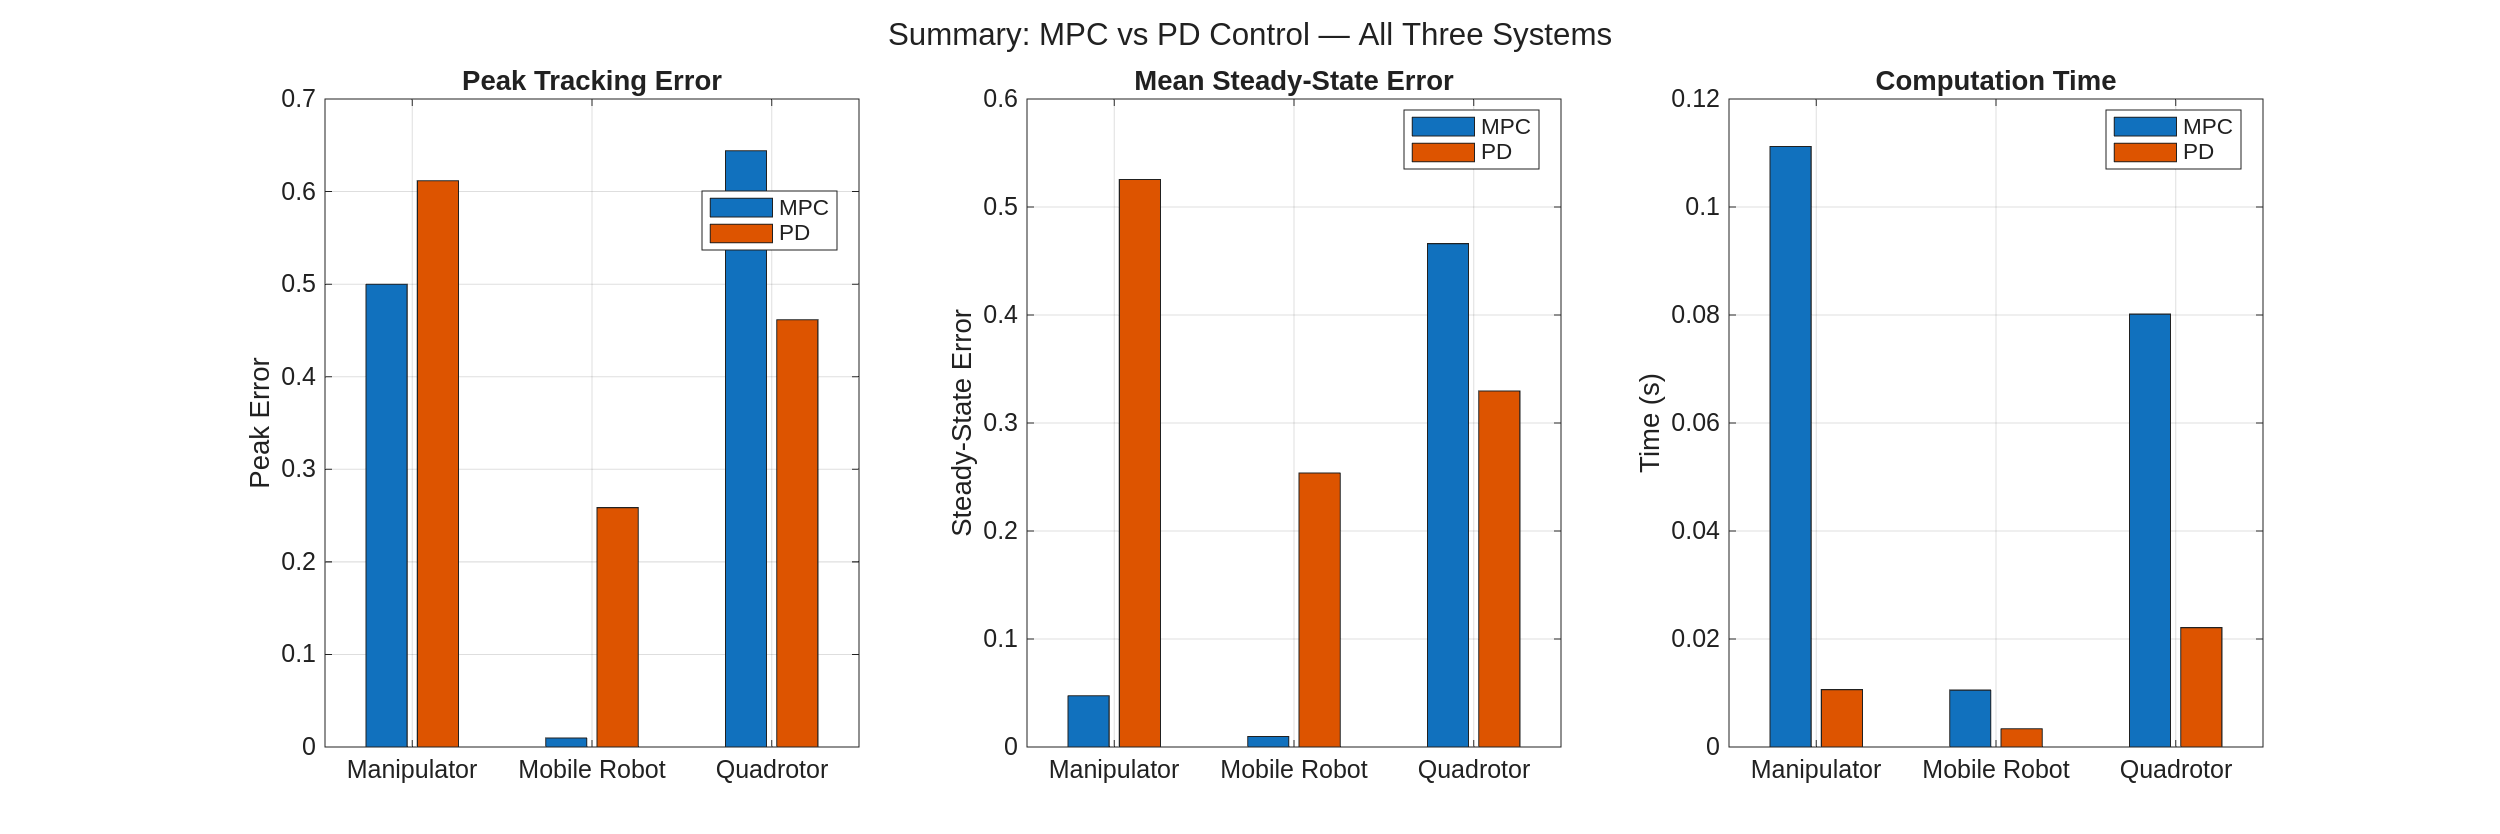
\includegraphics[width=0.92\textwidth,keepaspectratio]{images/week_03/Summary_MPC_vs_PD_for_All_Systems.png}
    \caption{Summary MPC vs PD for all systems.}
\end{figure}

\begin{figure}[ht]
    \centering
    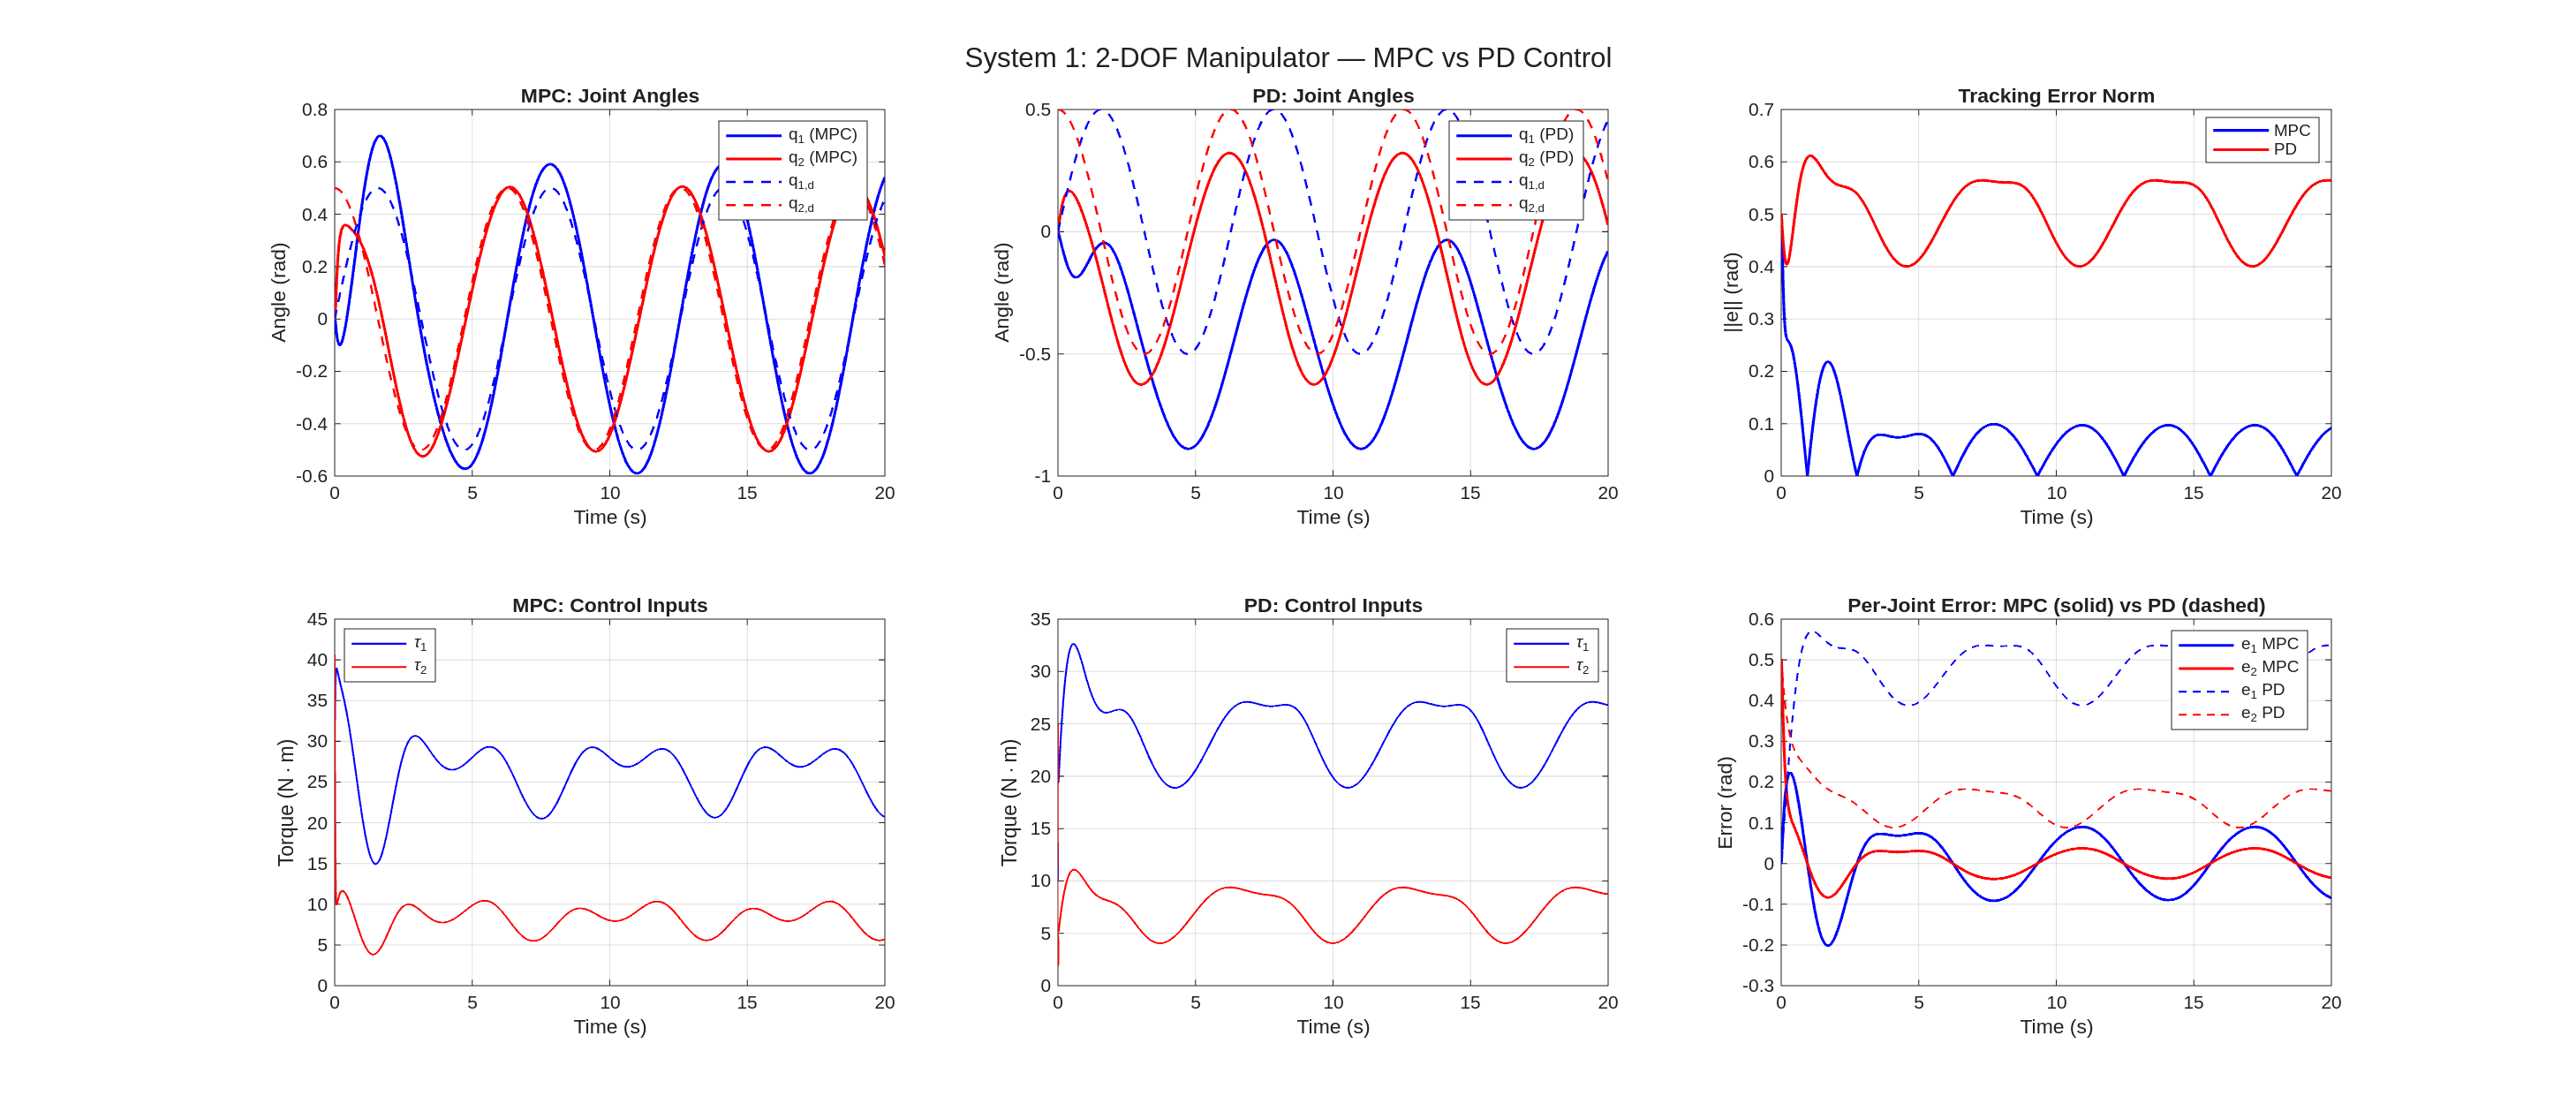
\includegraphics[width=0.92\textwidth,keepaspectratio]{images/week_03/System_1_2-DOF_Manipulator_MPC_vs_PD.png}
    \caption{System 1 2 DOF manipulator MPC vs PD.}
\end{figure}

\begin{figure}[ht]
    \centering
    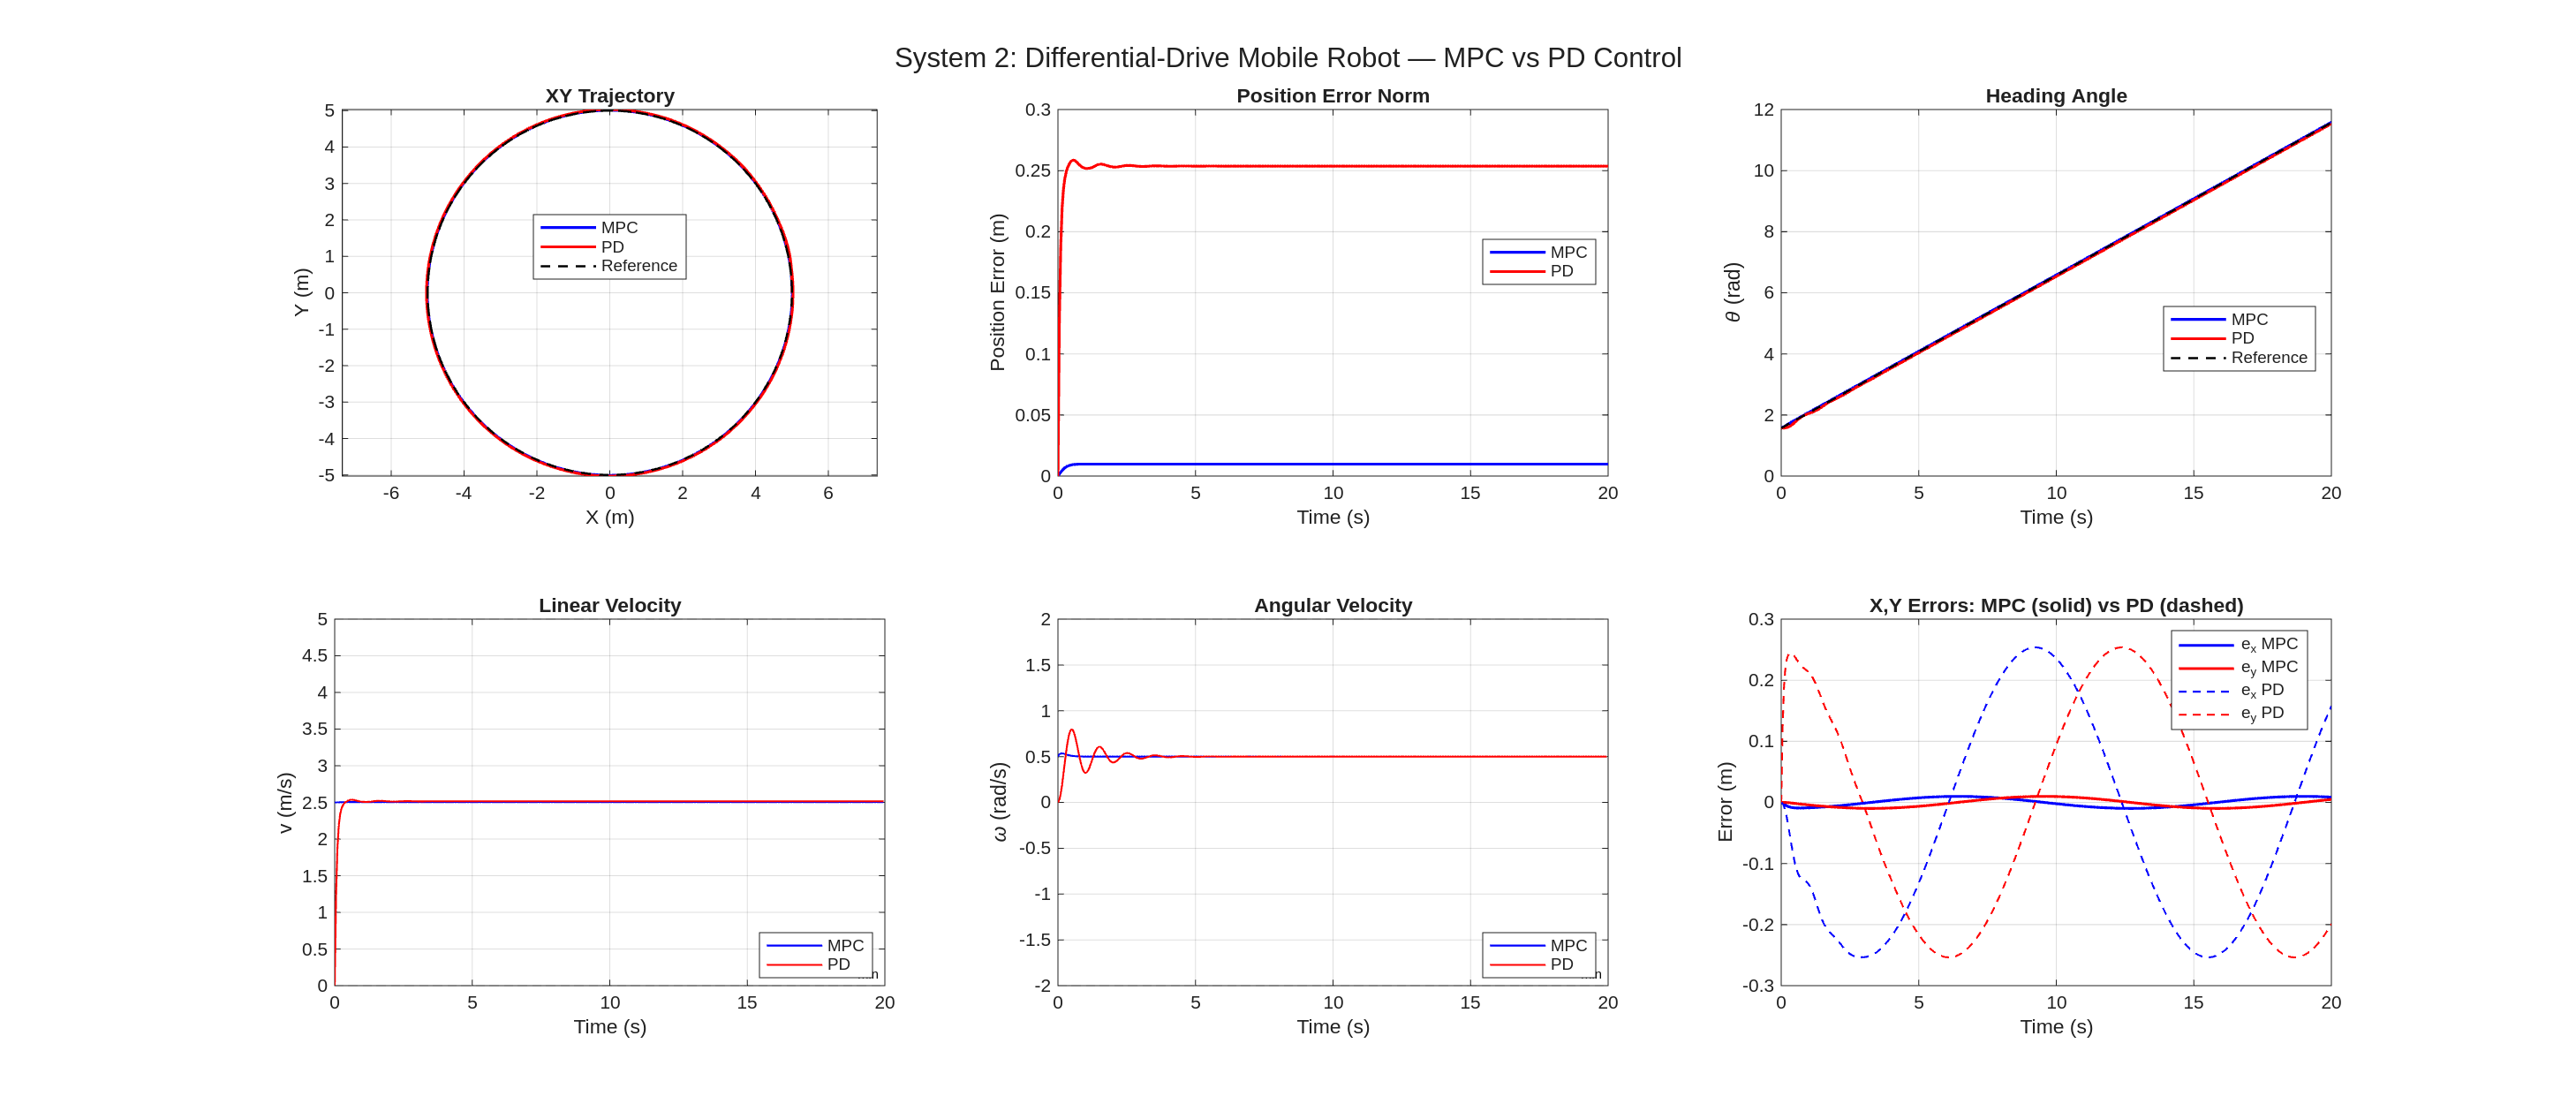
\includegraphics[width=0.92\textwidth,keepaspectratio]{images/week_03/System_2_Mobile_Robot_MPC_vs_PD.png}
    \caption{System 2 mobile robot MPC vs PD.}
\end{figure}

\begin{figure}[ht]
    \centering
    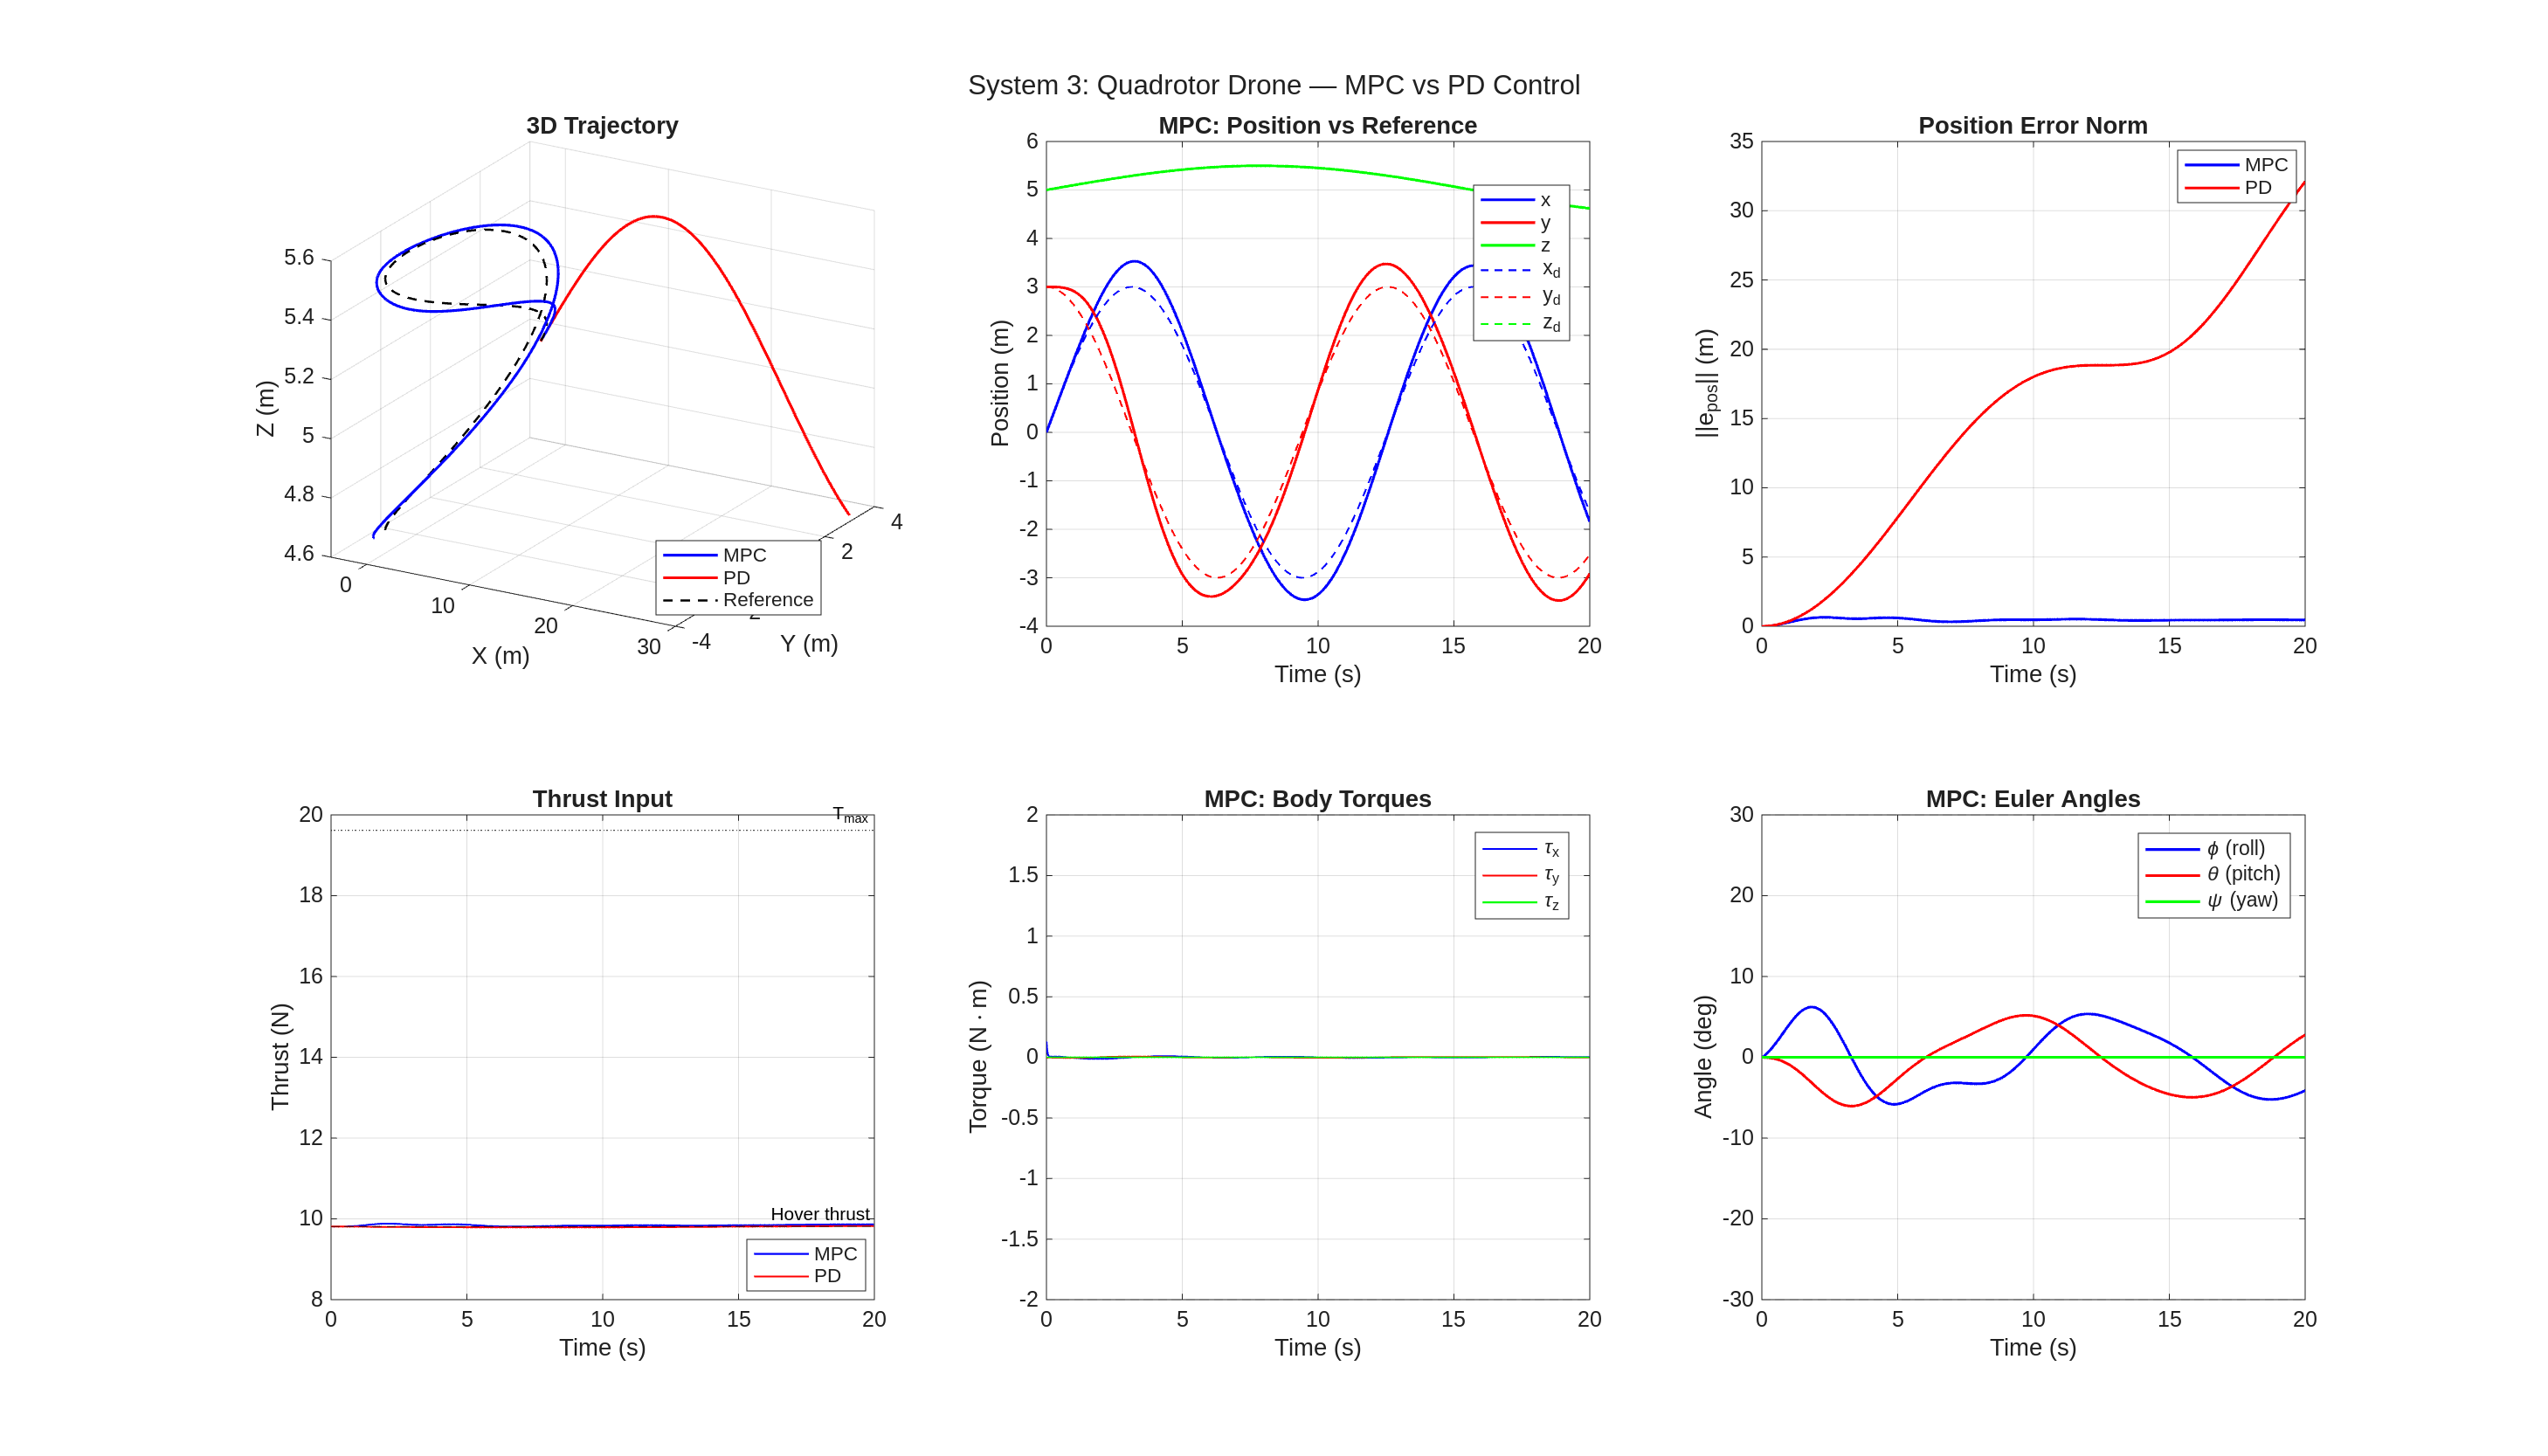
\includegraphics[width=0.92\textwidth,keepaspectratio]{images/week_03/System_3_Quadrotor_MPC_vs_PD.png}
    \caption{System 3 quadrotor MPC vs PD.}
\end{figure}

\section{Summary and Next Steps}

\subsection{Summary \& Key Takeaways}

\subsection{Core MPC Equations}

\begingroup\footnotesize
\begin{longtable}[]{@{}ll@{}}
\toprule\noalign{}
Equation & Description \\
\midrule\noalign{}
\endhead
\bottomrule\noalign{}
\endlastfoot
\(x_{k+1} = A\,x_k + B\,u_k\) & Discrete-time linear system model \\
\(\mathbf{X} = \mathcal{A}\,x_k + \mathcal{B}\,\mathbf{U}\) & Stacked state prediction over horizon \(N\) \\
\(J = (\mathbf{X} - \mathbf{X}_{\text{ref}})^T \mathbf{Q}_N (\mathbf{X} - \mathbf{X}_{\text{ref}}) + \mathbf{U}^T \mathbf{R}_N \mathbf{U}\) & Quadratic cost function \\
\(\mathbf{U}^* = (\mathcal{B}^T \mathbf{Q}_N \mathcal{B} + \mathbf{R}_N)^{-1} \mathcal{B}^T \mathbf{Q}_N (\mathbf{X}_{\text{ref}} - \mathcal{A}\,x_k)\) & Optimal control law (unconstrained) \\
\(u_k = \mathbf{U}^*(1{:}m)\) & Receding horizon: apply only first input \\
\end{longtable}\endgroup

\subsection{MPC vs Computed Torque Control}

\begingroup\footnotesize
\begin{longtable}[]{@{}lll@{}}
\toprule\noalign{}
Property & MPC & Computed Torque \\
\midrule\noalign{}
\endhead
\bottomrule\noalign{}
\endlastfoot
\textbf{Model Knowledge} & Requires linear (or nonlinear) model; can use approximate models with re-linearisation & Requires full nonlinear dynamics \(M(q)\), \(C(q,\dot{q})\), \(G(q)\) \\
\textbf{Constraint Handling} & Systematically incorporates state and control constraints in the optimisation & No built-in constraint handling; requires ad-hoc saturation or anti-windup \\
\textbf{Computation} & Solves a QP at every time step; computational cost grows with \(N\), \(n\), \(m\) & Evaluates \(M\), \(C\), \(G\) and a matrix-vector product; very fast per step \\
\textbf{Tracking Accuracy} & Optimal within the prediction horizon; slightly conservative due to linearisation & Perfect tracking with exact model (nonlinear cancellation) \\
\textbf{Multi-Objective} & Naturally balances tracking, energy, and constraints through cost weights & Single objective: tracking error minimisation \\
\textbf{Robustness} & Feedback through receding horizon; can incorporate robust/stochastic extensions & Sensitive to model mismatch; requires additional robust terms \\
\textbf{Best For} & Systems with constraints, slow-medium dynamics, trajectory optimisation & Fast manipulator control with known dynamics, high-rate servo loops \\
\end{longtable}\endgroup

\subsubsection{Key Takeaway 1}

MPC converts the control problem into a \textbf{repeated optimisation} problem. The quality of the controller depends directly on the quality of the model and the tuning of \(N\), \(Q\), \(R\).

\subsubsection{Key Takeaway 2}

The receding-horizon strategy provides \textbf{implicit feedback}: by re-solving at every step, MPC naturally rejects disturbances and compensates for model errors.

\subsubsection{Key Takeaway 3}

MPC\textquotesingle s greatest strength over computed torque is \textbf{constraint handling}. Real actuators have limits; MPC respects them by design.

\subsubsection{Key Takeaway 4}

Computed torque remains superior when the dynamics are well-known and the control loop must run at \textbf{very high rates} (\textgreater{} 1 kHz) where solving a QP is too expensive.

\subsection{Next Week: Adaptive Control}

\textbf{Building on Weeks 1 and 2, we will cover:}

\begin{itemize}
\tightlist
\item
  Parameter estimation and adaptive control for manipulators with unknown dynamics
\item
  Model Reference Adaptive Control (MRAC)
\item
  Linearity-in-parameters and the adaptive computed torque controller
\item
  Stability proofs for adaptive systems using Lyapunov-based methods
\end{itemize}

\subsection{Preparation}

\begin{itemize}
\tightlist
\item
  Complete all MATLAB activities from today and save your scripts
\item
  Review the linearity-in-parameters property from Week 1 (Section 1.4, Property 3)
\item
  Think about: \emph{"If the controller does not know \(M(q)\), \(C(q,\dot{q})\), or \(G(q)\), how could it learn these online while still maintaining stability?"}
\item
  Read about parameter convergence and persistent excitation
\end{itemize}

\textbf{Control for Robots}

Advanced Robotics Programme \textbar{} Academic Year 2025--26

Week 2: Model Predictive Control (MPC)

This lecture material is for educational use only.

% ----- auto-generated from week_04/Week*.html via pandoc -----
\chapter{Adaptive Control (Week 4)}
\labch{week_04}



Lyapunov-Based Adaptive Control for Robotic Systems with Parametric Uncertainty

M.Sc. Control for Robots --- AY 2025--26\\
3-Hour Lecture \& Lab • Week 4 of 12

\section{Overview}

\subsection{Week 3 Recall --- Model Predictive Control --- Exam Practice}

Before we begin new material, spend 20 minutes working through these two exam-style questions that cover last week\textquotesingle s MPC content. Write your solutions on paper.

\subsubsection{Question 1 --- MPC Problem Formulation \& Lifted Form (10 marks)}

Consider a discrete-time linear time-invariant system:

\[
                    x_{k+1} = A\,x_k + B\,u_k
                \]

with state \(x_k \in \mathbb{R}^n\), control \(u_k \in \mathbb{R}^m\), and a finite prediction horizon \(N\). The MPC cost function is:

\[
                    J = \sum_{i=0}^{N-1}\Big[\big(x_{k+i} - x_{\mathrm{ref}}\big)^T Q \big(x_{k+i} - x_{\mathrm{ref}}\big) + u_{k+i}^T R\, u_{k+i}\Big]
                \]

where \(Q \succeq 0\) and \(R \succ 0\).

\textbf{(a)} By recursive substitution, show that the predicted state sequence can be written in compact (lifted) form as:

\[
                    \mathbf{X} = \mathcal{A}\,x_k + \mathcal{B}\,\mathbf{U}
                \]

where the stacked vectors are \(\mathbf{X} = \begin{bmatrix} x_{k+1} \\ x_{k+2} \\ \vdots \\ x_{k+N} \end{bmatrix}\) and \(\mathbf{U} = \begin{bmatrix} u_k \\ u_{k+1} \\ \vdots \\ u_{k+N-1} \end{bmatrix}\), and derive the explicit forms:

\[
                    \mathcal{A} = \begin{bmatrix} A \\ A^2 \\ A^3 \\ \vdots \\ A^N \end{bmatrix}, \qquad
                    \mathcal{B} = \begin{bmatrix}
                        B & 0 & 0 & \cdots & 0 \\
                        AB & B & 0 & \cdots & 0 \\
                        A^2B & AB & B & \cdots & 0 \\
                        \vdots & \vdots & \vdots & \ddots & \vdots \\
                        A^{N-1}B & A^{N-2}B & A^{N-3}B & \cdots & B
                    \end{bmatrix}
                \]

Show every substitution step from \(i=1\) to \(i=N\).

\textbf{(b)} Identify the structure of \(\mathcal{B}\) (lower-triangular block Toeplitz). Explain why this structure arises from the causal nature of the system (future states depend only on past and present inputs).

\subsubsection{Question 2 --- Deriving the Optimal MPC Control Law (10 marks)}

Starting from the lifted quadratic cost:

\[
                    J = \big(\mathbf{X} - \mathbf{X}_{\mathrm{ref}}\big)^T \bar{Q}\,\big(\mathbf{X} - \mathbf{X}_{\mathrm{ref}}\big) + \mathbf{U}^T \bar{R}\,\mathbf{U}
                \]

where \(\bar{Q} = \mathrm{blkdiag}(Q, Q, \dots, Q) \in \mathbb{R}^{nN \times nN}\) and \(\bar{R} = \mathrm{blkdiag}(R, R, \dots, R) \in \mathbb{R}^{mN \times mN}\):

\textbf{(a)} Substitute \(\mathbf{X} = \mathcal{A}\,x_k + \mathcal{B}\,\mathbf{U}\) into \(J\) and expand fully:

\[
                    J = \big(\mathcal{A}\,x_k + \mathcal{B}\,\mathbf{U} - \mathbf{X}_{\mathrm{ref}}\big)^T \bar{Q}\,\big(\mathcal{A}\,x_k + \mathcal{B}\,\mathbf{U} - \mathbf{X}_{\mathrm{ref}}\big) + \mathbf{U}^T \bar{R}\,\mathbf{U}
                \]

Let \(\mathbf{E} = \mathbf{X}_{\mathrm{ref}} - \mathcal{A}\,x_k\). Show that:

\[
                    J = \mathbf{U}^T\!\big(\mathcal{B}^T \bar{Q}\,\mathcal{B} + \bar{R}\big)\mathbf{U} - 2\,\mathbf{E}^T \bar{Q}\,\mathcal{B}\,\mathbf{U} + \mathbf{E}^T \bar{Q}\,\mathbf{E}
                \]

\textbf{(b)} Take \(\frac{\partial J}{\partial \mathbf{U}} = 0\) and derive:

\[
                    \mathbf{U}^* = \big(\mathcal{B}^T \bar{Q}\,\mathcal{B} + \bar{R}\big)^{-1} \mathcal{B}^T \bar{Q}\,\big(\mathbf{X}_{\mathrm{ref}} - \mathcal{A}\,x_k\big)
                \]

\textbf{(c)} Define the MPC gain. Since only the first \(m\) rows of \(\mathbf{U}^*\) are applied (receding horizon), let \(E_1 = [I_m \;\; 0 \;\; \cdots \;\; 0]\). Then:

\[
                    u_k^* = E_1 \mathbf{U}^* = \underset{\text{\footnotesize K_{\mathrm{MPC,ref}}}}{\underline{E_1 \big(\mathcal{B}^T \bar{Q}\,\mathcal{B} + \bar{R}\big)^{-1} \mathcal{B}^T \bar{Q}}}\,\mathbf{X}_{\mathrm{ref}} - \underset{\text{\footnotesize K_{\mathrm{MPC}}}}{\underline{E_1 \big(\mathcal{B}^T \bar{Q}\,\mathcal{B} + \bar{R}\big)^{-1} \mathcal{B}^T \bar{Q}\,\mathcal{A}}}\,x_k
                \]

Explain why \(K_{\mathrm{MPC}}\) is a state-feedback gain and how increasing \(R\) relative to \(Q\) affects the control aggressiveness.

\textbf{Time limit: 20 minutes.} This is exactly the format and difficulty level you will encounter in the final exam. Write full derivations showing every step. Partial credit is awarded for correct intermediate work.

\subsection{Learning Outcomes}

\begin{itemize}
\tightlist
\item
  Understand why adaptive control is needed when system parameters are unknown or time-varying, and articulate the limitations of computed torque and MPC that assume known models.
\item
  Derive the adaptive control law using Lyapunov-based stability analysis, including the construction of a candidate Lyapunov function and verification that its time derivative is negative semi-definite.
\item
  Apply the linearity-in-parameters property of rigid-body dynamics: \(M(q)\ddot{q} + C(q,\dot{q})\dot{q} + G(q) = Y(q, \dot{q}, \ddot{q})\,\theta\), identifying the regressor matrix \(Y\) and parameter vector \(\theta\) for specific systems.
\item
  Implement adaptive control for three robotic platforms: a 2-DOF manipulator, a differential-drive mobile robot, and a quadrotor UAV.
\item
  Simulate and compare the performance of fixed-model computed torque control versus adaptive control under parameter uncertainty, demonstrating convergence of parameter estimates.
\end{itemize}

\section{Adaptive Control Theory}

\subsection{Why Adaptive Control?}

In Week 1, we designed a computed torque controller for a 2-DOF manipulator. The control law was:

\[
                \tau = M(q)\big(\ddot{q}_d + K_v\dot{e} + K_p e\big) + C(q,\dot{q})\dot{q} + G(q)
            \]

This requires \textbf{exact knowledge} of the inertia matrix \(M(q)\), Coriolis/centrifugal matrix \(C(q,\dot{q})\), and gravity vector \(G(q)\). In practice, this assumption fails for several reasons:

\begin{itemize}
\tightlist
\item
  \textbf{Unknown payloads:} A manipulator picks up objects of unknown mass. The effective \(m_2\) changes.
\item
  \textbf{Manufacturing tolerances:} Link lengths, masses, and centres of gravity are only approximately known.
\item
  \textbf{Wear and degradation:} Friction coefficients, gear ratios, and joint stiffness change over time.
\item
  \textbf{Model simplification:} We ignore link flexibility, actuator dynamics, and higher-order effects.
\end{itemize}

\textbf{Key insight:} If the model parameters used in computed torque are wrong, the nonlinear cancellation is imperfect, and the closed-loop system is no longer a simple linear error system. Tracking performance degrades, and stability may be lost.

Adaptive control addresses this by estimating the unknown parameters online, while simultaneously controlling the system. The parameter estimates converge to values that ensure good tracking, even if the true parameters are never exactly identified.

\textbf{Figure 1:} Adaptive control block diagram. The {blue control loop} tracks the reference, while the {orange adaptation loop} estimates unknown plant parameters and feeds them to the controller.

\textbf{Figure 2:} Comparison of {Direct} and {Indirect} adaptive control. In direct adaptation, the error signal is fed to an adaptation law that adjusts controller gains K(t) directly. In indirect adaptation, the error drives a parameter estimator to obtain θ̂, which is then used in a gain computation step to determine K(θ̂).

\subsection{The Linearity-in-Parameters Property}

The dynamics of a rigid-body robotic system can always be written as:

\(M(q)\ddot{q} + C(q,\dot{q})\dot{q} + G(q) = Y(q, \dot{q}, \ddot{q})\,\theta\)

where:

\begin{itemize}
\tightlist
\item
  \(Y(q, \dot{q}, \ddot{q}) \in \mathbb{R}^{n \times p}\) is the \textbf{regressor matrix} --- a known matrix that depends on joint positions, velocities, and accelerations, but \emph{not} on the unknown parameters.
\item
  \(\theta \in \mathbb{R}^p\) is the \textbf{parameter vector} --- a constant vector containing all the unknown dynamic parameters (products of masses, lengths, inertias, friction coefficients, etc.).
\end{itemize}

This is the \emph{linearity-in-parameters} property. It holds because the equations of motion are derived from the Lagrangian, which is quadratic in velocities and linear in the inertial parameters. The property is fundamental to adaptive control: it allows us to separate what we know (the structure of \(Y\)) from what we do not know (the values in \(\theta\)).

\textbf{Figure 3:} The linearity-in-parameters property separates robot dynamics into a {known regressor matrix Y} (computable from kinematics) multiplied by an {unknown parameter vector θ} (to be estimated online).

\subsection{Concrete Example: 2-DOF Planar Manipulator}

\textbf{Figure 4:} 2-DOF planar manipulator. {Link 1} (length l₁, mass m₁) and {Link 2} (length l₂, mass m₂) rotate at joints with angles θ₁ and θ₂. Joint torques τ₁ and τ₂ are the control inputs.

Consider the 2-DOF planar manipulator with link masses \(m_1, m_2\), link lengths \(l_1, l_2\), and gravity \(g\). The standard Euler-Lagrange dynamics are:

\[
                M(q)\ddot{q} + C(q,\dot{q})\dot{q} + G(q) = \tau
            \]

with:

\[
                M(q) = \begin{bmatrix}
                    m_1 l_1^2 + m_2(l_1^2 + l_2^2 + 2l_1 l_2 \cos q_2) & m_2(l_2^2 + l_1 l_2 \cos q_2) \\
                    m_2(l_2^2 + l_1 l_2 \cos q_2) & m_2 l_2^2
                \end{bmatrix}
            \]
\[
                C(q,\dot{q}) = \begin{bmatrix}
                    -m_2 l_1 l_2 \sin(q_2)\,\dot{q}_2 & -m_2 l_1 l_2 \sin(q_2)(\dot{q}_1 + \dot{q}_2) \\
                    m_2 l_1 l_2 \sin(q_2)\,\dot{q}_1 & 0
                \end{bmatrix}
            \]
\[
                G(q) = \begin{bmatrix}
                    (m_1 + m_2)\,g\,l_1 \sin q_1 + m_2\,g\,l_2 \sin(q_1 + q_2) \\
                    m_2\,g\,l_2 \sin(q_1 + q_2)
                \end{bmatrix}
            \]

Define the parameter vector:

\[
                    \theta = \begin{bmatrix} \theta_1 \\ \theta_2 \\ \theta_3 \\ \theta_4 \\ \theta_5 \\ \theta_6 \end{bmatrix}
                    = \begin{bmatrix} m_1 l_1^2 \\ m_2 l_1^2 \\ m_2 l_2^2 \\ m_2 l_1 l_2 \\ (m_1 + m_2)\,g\,l_1 \\ m_2\,g\,l_2 \end{bmatrix}
                \]

Then the regressor matrix \(Y \in \mathbb{R}^{2 \times 6}\) such that \(\tau = Y(q, \dot{q}, \ddot{q})\,\theta\) is:

\[
                    Y = \begin{bmatrix}
                        \ddot{q}_1 & \ddot{q}_1 & \ddot{q}_1 + \ddot{q}_2 & 2\cos(q_2)\ddot{q}_1 + \cos(q_2)\ddot{q}_2 - \sin(q_2)\dot{q}_2\dot{q}_1 - \sin(q_2)(\dot{q}_1+\dot{q}_2)\dot{q}_2 & \sin(q_1) & \sin(q_1+q_2) \\
                        0 & 0 & \ddot{q}_1 + \ddot{q}_2 & \cos(q_2)\ddot{q}_1 + \sin(q_2)\dot{q}_1^2 & 0 & \sin(q_1+q_2)
                    \end{bmatrix}
                \]

You can verify: multiply \(Y\theta\) and recover exactly \(M(q)\ddot{q} + C(q,\dot{q})\dot{q} + G(q)\). Every entry of \(Y\) is computable from measured (or commanded) \(q, \dot{q}, \ddot{q}\).

\subsection{The Adaptive Control Law}

We now construct the adaptive controller. Define the tracking error and its filtered version:

\[
                    e = q_d - q, \qquad \dot{e} = \dot{q}_d - \dot{q}
                \]

Define the \textbf{sliding variable} (composite error):

\[
                    s = \dot{e} + \Lambda\, e
                \]

where \(\Lambda = \Lambda^T \succ 0\) is a positive definite design matrix. Equivalently, define the \textbf{reference velocity} and \textbf{reference acceleration}:

\[
                \dot{q}_r = \dot{q}_d + \Lambda\,e = \dot{q} + s
            \]
\[
                \ddot{q}_r = \ddot{q}_d + \Lambda\,\dot{e}
            \]

Notice that \(s = \dot{q}_r - \dot{q}\), so \(s \to 0\) implies \(\dot{q} \to \dot{q}_r\), which combined with the definition of \(\dot{q}_r\) implies both \(e \to 0\) and \(\dot{e} \to 0\) exponentially (since \(\dot{e} + \Lambda e = 0\) is a stable linear ODE).

The \textbf{adaptive control law} is:

\(\tau = Y(q, \dot{q}, \dot{q}_r, \ddot{q}_r)\,\hat{\theta} + K_D\, s\)

where:

\begin{itemize}
\tightlist
\item
  \(\hat{\theta}\) is the current estimate of the parameter vector \(\theta\).
\item
  \(Y(q, \dot{q}, \dot{q}_r, \ddot{q}_r)\) is the regressor evaluated at the \emph{reference} velocity and acceleration (not the actual \(\ddot{q}\), which we cannot measure cleanly).
\item
  \(K_D = K_D^T \succ 0\) is a positive definite gain matrix providing damping on the sliding variable.
\end{itemize}

\textbf{Important subtlety:} We evaluate the regressor at \((\dot{q}_r, \ddot{q}_r)\) instead of \((\dot{q}, \ddot{q})\). This avoids the need to measure or numerically differentiate joint accelerations, and it ensures that the regressor is known (computable from \(q, \dot{q}, q_d, \dot{q}_d, \ddot{q}_d\)).

\subsection{Parameter Update Law}

The parameter estimates are updated according to:

\(\dot{\hat{\theta}} = \Gamma^{-1}\, Y^T\! s\)

where \(\Gamma = \Gamma^T \succ 0\) is the \textbf{adaptation gain matrix}. Define the parameter estimation error:

\[
                \tilde{\theta} = \hat{\theta} - \theta
            \]

Since \(\theta\) is constant, \(\dot{\tilde{\theta}} = \dot{\hat{\theta}}\).

\textbf{Figure 8:} Parameter convergence under adaptive control. Multiple parameter estimates starting from different initial conditions all converge toward the true parameter value θ* (dashed line). The adaptation law drives estimates toward values that minimize tracking error.

\subsection{Lyapunov Stability Proof}

\subsubsection{Theorem (Adaptive Control Stability)}

Under the adaptive control law \(\tau = Y\hat{\theta} + K_D s\) with the update law \(\dot{\hat{\theta}} = \Gamma^{-1} Y^T s\), the sliding variable \(s \to 0\) and consequently the tracking errors \(e \to 0\), \(\dot{e} \to 0\) as \(t \to \infty\).

\textbf{Figure 7:} Lyapunov stability concept. Left: the Lyapunov function V forms a bowl-shaped surface, and the system trajectory (pink spiral) descends toward the equilibrium. Right: V(t) monotonically decreases over time since V̇ = -sᵀK₄s is always non-positive.

\textbf{Proof.} Define the candidate Lyapunov function:

\[
                V = \frac{1}{2}\,s^T M(q)\,s + \frac{1}{2}\,\tilde{\theta}^T \Gamma\,\tilde{\theta}
            \]

Since \(M(q) \succ 0\) and \(\Gamma \succ 0\), both terms are strictly positive for \((s, \tilde{\theta}) \neq (0,0)\), so \(V\) is a valid positive definite candidate with \(V = 0\) iff \(s = 0\) and \(\tilde{\theta} = 0\).

\textbf{Step 1: Time derivative of \(V\).}

\[
                \dot{V} = s^T M(q)\,\dot{s} + \frac{1}{2}\,s^T \dot{M}(q)\,s + \tilde{\theta}^T \Gamma\,\dot{\tilde{\theta}}
            \]

\textbf{Step 2: Simplify \(s^T M\dot{s} + \tfrac{1}{2}s^T\dot{M}s\) using skew-symmetry.}\\
The Euler-Lagrange formulation guarantees that \(N := \dot{M} - 2C\) is skew-symmetric, i.e.\textbackslash{} \(s^T N s = 0\) for all \(s\). This gives \(\tfrac{1}{2}s^T\dot{M}s = s^T C s\), so:
\[
                s^T M\dot{s} + \tfrac{1}{2}s^T\dot{M}s = s^T(M\dot{s} + Cs)
            \]

\textbf{Step 3: Evaluate \(M\dot{s} + Cs\).}\\
Since \(s = \dot{q}_r - \dot{q}\), we have \(\dot{s} = \ddot{q}_r - \ddot{q}\). Substituting \(M\ddot{q} = \tau - C\dot{q} - G\):
\[
                M\dot{s} + Cs = M\ddot{q}_r - M\ddot{q} + Cs = M\ddot{q}_r + C\dot{q} + G - \tau + C(\dot{q}_r - \dot{q})
                = M\ddot{q}_r + C\dot{q}_r + G - \tau
            \]
By linearity-in-parameters, \(M\ddot{q}_r + C\dot{q}_r + G = Y\theta\). Substituting the control law \(\tau = Y\hat{\theta} + K_D s\):
\[
                M\dot{s} + Cs = Y\theta - Y\hat{\theta} - K_D s = -Y(\hat{\theta} - \theta) - K_D s = -Y\tilde{\theta} - K_D s
            \]

\textbf{Step 4: Substitute back into \(\dot{V}\).}

\[
                \dot{V} = s^T(-Y\tilde{\theta} - K_D s) + \tilde{\theta}^T \Gamma\,\dot{\tilde{\theta}}
                = -s^T Y\tilde{\theta} - s^T K_D s + \tilde{\theta}^T \Gamma\,\dot{\tilde{\theta}}
            \]

\textbf{Step 5: Cancel the cross term using the update law.}\\
Substitute \(\dot{\tilde{\theta}} = \dot{\hat{\theta}} = \Gamma^{-1}Y^T s\):
\[
                \tilde{\theta}^T \Gamma\,\dot{\tilde{\theta}} = \tilde{\theta}^T \Gamma\,(\Gamma^{-1}Y^T s) = \tilde{\theta}^T Y^T s = (Y\tilde{\theta})^T s = s^T Y\tilde{\theta}
            \]
The cross terms cancel exactly:
\[
                \dot{V} = -s^T Y\tilde{\theta} - s^T K_D s + s^T Y\tilde{\theta} = -s^T K_D s
            \]

\textbf{Result:}
\[
                    \boxed{\dot{V} = -s^T K_D\, s \leq 0}
                \]
Since \(K_D \succ 0\), we have \(\dot{V} < 0\) whenever \(s \neq 0\), so \(V\) is non-increasing and bounded below by zero. By Barbalat\textquotesingle s lemma, \(s(t) \to 0\) as \(t \to \infty\). Since \(s = \dot{e} + \Lambda e\) with \(\Lambda \succ 0\), this implies \(e(t) \to 0\) and \(\dot{e}(t) \to 0\). \(\square\)

\textbf{Sign convention.} We define \(\tilde{\theta} = \hat{\theta} - \theta\), so \(\dot{\tilde{\theta}} = \dot{\hat{\theta}}\). The Lyapunov weight on the parameter error term is \(\Gamma\) (not \(\Gamma^{-1}\)), which is why the update law \(\dot{\hat{\theta}} = \Gamma^{-1}Y^T s\) produces the exact cancellation \(\tilde{\theta}^T\Gamma(\Gamma^{-1}Y^T s) = s^T Y\tilde{\theta}\). Some textbooks define \(\tilde{\theta} = \theta - \hat{\theta}\); with that reversed convention the update law carries a negative sign, but the underlying physics is identical.

\textbf{Result:}
\[
                    \boxed{\dot{V} = -s^T K_D\, s \leq 0}
                \]
Since \(K_D \succ 0\), \(\dot{V} < 0\) whenever \(s \neq 0\). By Barbalat\textquotesingle s lemma, \(s(t) \to 0\) as \(t \to \infty\). Since \(s = \dot{e} + \Lambda e\) and \(\Lambda \succ 0\), this implies \(e(t) \to 0\) and \(\dot{e}(t) \to 0\).

\textbf{Sign convention note:} We use \(\tilde{\theta} = \hat{\theta} - \theta\), so \(\dot{\tilde{\theta}} = \dot{\hat{\theta}}\). With the Lyapunov function \(V = \tfrac{1}{2}s^T M s + \tfrac{1}{2}\tilde{\theta}^T\Gamma\tilde{\theta}\), the update law that cancels the cross term is:
\[
                    \dot{\hat{\theta}} = \Gamma^{-1}\,Y^T\!s
                \]
Some textbooks define \(\tilde{\theta} = \theta - \hat{\theta}\) (reversed). With that convention \(\dot{\tilde{\theta}} = -\dot{\hat{\theta}}\), and the update law is written as \(\dot{\hat{\theta}} = \Gamma^{-1} Y^T s\) with opposite sign in the cancellation. The physics is identical; only the bookkeeping differs. Always check which definition of \(\tilde{\theta}\) a textbook uses before comparing formulas.

\subsubsection{Think-Pair-Share: Effect of Adaptation Gain}

Consider the adaptation gain matrix \(\Gamma\). Discuss with your neighbour:

\begin{enumerate}
\tightlist
\item
  What happens if \(\Gamma\) is very large (fast adaptation)?

  \begin{itemize}
  \tightlist
  \item
    Parameter estimates change rapidly, which can cause large transient oscillations and potentially excite unmodelled dynamics. In the worst case, the system becomes unstable in practice (even though the theory guarantees stability for the nominal model).
  \end{itemize}
\item
  What happens if \(\Gamma\) is very small (slow adaptation)?

  \begin{itemize}
  \tightlist
  \item
    Parameters converge very slowly. The controller behaves essentially like a PD controller (the \(K_D s\) term dominates) until the parameters have time to converge. Tracking errors may remain large for an extended period.
  \end{itemize}
\item
  Does the Lyapunov proof guarantee that \(\hat{\theta} \to \theta\)?

  \begin{itemize}
  \tightlist
  \item
    No. The proof only guarantees \(s \to 0\) (and hence \(e \to 0\)). Parameter convergence requires \emph{persistent excitation} of the regressor. If the trajectory does not excite all modes, some parameters may not converge to their true values, but tracking performance is still guaranteed.
  \end{itemize}
\end{enumerate}

\section{Adaptive Control for 2-DOF Manipulator}

\subsection{System Setup}

We now implement the full adaptive controller for the 2-DOF planar manipulator from Section 3.3. The true parameters are:

\begin{table}[ht]\footnotesize\centering
\adjustbox{max width=\textwidth,max totalheight=0.85\textheight}{%
\begin{tabular}{llll}

\topruleParameter & Symbol & True Value & Initial Estimate \\
\midrule\bottomruleLink 1 mass & \(m_1\) & 1.0 kg & 1.0 kg (known) \\
Link 2 mass & \(m_2\) & 2.0 kg & 1.0 kg (50\% error) \\
Link 1 length & \(l_1\) & 1.0 m & 1.0 m (known) \\
Link 2 length & \(l_2\) & 1.0 m & 1.0 m (known) \\
Gravity & \(g\) & 9.81 m/s² & 9.81 m/s² (known) \\
\end{tabular}}
\end{table}


Even though only \(m_2\) is wrong, all composite parameters involving \(m_2\) are affected:

\begin{table}[ht]\footnotesize\centering
\adjustbox{max width=\textwidth,max totalheight=0.85\textheight}{%
\begin{tabular}{lll}

\topruleComposite Parameter & True Value & Initial Estimate \\
\midrule\bottomrule\(\theta_1 = m_1 l_1^2\) & 1.0 & 1.0 \\
\(\theta_2 = m_2 l_1^2\) & 2.0 & 1.0 \\
\(\theta_3 = m_2 l_2^2\) & 2.0 & 1.0 \\
\(\theta_4 = m_2 l_1 l_2\) & 2.0 & 1.0 \\
\(\theta_5 = (m_1+m_2)gl_1\) & 29.43 & 19.62 \\
\(\theta_6 = m_2 g l_2\) & 19.62 & 9.81 \\
\end{tabular}}
\end{table}


\subsection{Building the Regressor Matrix}

We need the regressor evaluated at the reference quantities \((\dot{q}_r, \ddot{q}_r)\) instead of \((\dot{q}, \ddot{q})\). Define:

\[
                \dot{q}_r = \dot{q}_d + \Lambda(q_d - q), \qquad \ddot{q}_r = \ddot{q}_d + \Lambda(\dot{q}_d - \dot{q})
            \]

The regressor \(Y(q, \dot{q}, \dot{q}_r, \ddot{q}_r) \in \mathbb{R}^{2 \times 6}\) is constructed by replacing every occurrence of \(\ddot{q}\) with \(\ddot{q}_r\) and every occurrence of \(\dot{q}\) in the Coriolis terms with a mix of \(\dot{q}\) and \(\dot{q}_r\) as appropriate. Specifically:

\[
                Y_{11} = \ddot{q}_{r1}
            \]
\[
                Y_{12} = \ddot{q}_{r1}
            \]
\[
                Y_{13} = \ddot{q}_{r1} + \ddot{q}_{r2}
            \]
\[
                Y_{14} = 2\cos(q_2)\ddot{q}_{r1} + \cos(q_2)\ddot{q}_{r2} - \sin(q_2)\dot{q}_2\dot{q}_{r1} - \sin(q_2)(\dot{q}_1 + \dot{q}_2)\dot{q}_{r2}
            \]
\[
                Y_{15} = \sin(q_1)
            \]
\[
                Y_{16} = \sin(q_1 + q_2)
            \]
\[
                Y_{21} = 0
            \]
\[
                Y_{22} = 0
            \]
\[
                Y_{23} = \ddot{q}_{r1} + \ddot{q}_{r2}
            \]
\[
                Y_{24} = \cos(q_2)\ddot{q}_{r1} + \sin(q_2)\dot{q}_1 \dot{q}_{r1}
            \]
\[
                Y_{25} = 0
            \]
\[
                Y_{26} = \sin(q_1 + q_2)
            \]

\subsection{Complete Control Algorithm}

\begin{verbatim}
                Algorithm: Adaptive Control for 2-DOF Manipulator
\end{verbatim}

\textbf{Given:} desired trajectory q\_d(t), dq\_d(t), ddq\_d(t)
\textbf{Initialise:} theta\_hat = theta\_hat\_0 (initial parameter estimates)
\textbf{Design parameters:} Lambda, K\_D, Gamma (all positive definite)
\textbf{At each time step:}
1. Measure q, dq
2. Compute errors:
e = q\_d - q
de = dq\_d - dq
3. Compute reference signals:
dq\_r = dq\_d + Lambda * e
ddq\_r = ddq\_d + Lambda * de
4. Compute sliding variable:
s = de + Lambda * e (equivalently s = dq\_r - dq)
5. Build regressor Y(q, dq, dq\_r, ddq\_r) {[}2x6 matrix{]}
6. Compute control torque:
tau = Y * theta\_hat + K\_D * s
7. Update parameter estimates:
d(theta\_hat)/dt = Gamma\_inv * Y\textquotesingle{} * s
8. Apply tau to the plant

\subsection{MATLAB Implementation}

\begin{lstlisting}[language=Matlab]
%% Adaptive Control for 2-DOF Manipulator
% True parameters
m1 = 1; m2 = 2; l1 = 1; l2 = 1; g = 9.81;
theta_true = [m1*l1^2; m2*l1^2; m2*l2^2; m2*l1*l2; (m1+m2)*g*l1; m2*g*l2];

% Initial estimates (m2_hat = 1 instead of 2)
m2_hat = 1;
theta_hat0 = [m1*l1^2; m2_hat*l1^2; m2_hat*l2^2; m2_hat*l1*l2; ...
              (m1+m2_hat)*g*l1; m2_hat*g*l2];

% Design parameters
Lambda = 10*eye(2);    % Sliding surface slope
K_D    = 50*eye(2);    % Damping gain
Gamma_inv = 5*eye(6);  % Inverse adaptation gain

% Desired trajectory
qd   = @(t) [0.5*sin(t); 0.5*cos(t)];
dqd  = @(t) [0.5*cos(t); -0.5*sin(t)];
ddqd = @(t) [-0.5*sin(t); -0.5*cos(t)];

% State: [q1; q2; dq1; dq2; theta_hat(1:6)]
x0 = [0; 0; 0; 0; theta_hat0];
tspan = 0:0.01:20;

[t, X] = ode45(@(t,x) adaptive_manipulator(t, x, ...
    m1, m2, l1, l2, g, Lambda, K_D, Gamma_inv, qd, dqd, ddqd), tspan, x0);

function dx = adaptive_manipulator(t, x, m1, m2, l1, l2, g, ...
                                    Lambda, K_D, Gamma_inv, qd, dqd, ddqd)
    q  = x(1:2);  dq = x(3:4);  theta_hat = x(5:10);

    % True dynamics matrices
    c2 = cos(q(2)); s2 = sin(q(2));
    M = [m1*l1^2 + m2*(l1^2+l2^2+2*l1*l2*c2), m2*(l2^2+l1*l2*c2);
         m2*(l2^2+l1*l2*c2),                    m2*l2^2];
    C = [-m2*l1*l2*s2*dq(2), -m2*l1*l2*s2*(dq(1)+dq(2));
          m2*l1*l2*s2*dq(1),  0];
    G = [(m1+m2)*g*l1*sin(q(1)) + m2*g*l2*sin(q(1)+q(2));
          m2*g*l2*sin(q(1)+q(2))];

    % Errors and reference signals
    e   = qd(t) - q;
    de  = dqd(t) - dq;
    dqr  = dqd(t) + Lambda*e;
    ddqr = ddqd(t) + Lambda*de;
    s    = de + Lambda*e;

    % Build regressor Y(q, dq, dqr, ddqr) [2x6]
    s2q = sin(q(2)); c2q = cos(q(2));
    s1  = sin(q(1)); s12 = sin(q(1)+q(2));

    Y = zeros(2,6);
    Y(1,1) = ddqr(1);
    Y(1,2) = ddqr(1);
    Y(1,3) = ddqr(1) + ddqr(2);
    Y(1,4) = 2*c2q*ddqr(1) + c2q*ddqr(2) ...
             - s2q*dq(2)*dqr(1) - s2q*(dq(1)+dq(2))*dqr(2);
    Y(1,5) = s1;
    Y(1,6) = s12;
    Y(2,1) = 0;
    Y(2,2) = 0;
    Y(2,3) = ddqr(1) + ddqr(2);
    Y(2,4) = c2q*ddqr(1) + s2q*dq(1)*dqr(1);
    Y(2,5) = 0;
    Y(2,6) = s12;

    % Adaptive control law
    tau = Y*theta_hat + K_D*s;

    % Parameter update law
    dtheta_hat = Gamma_inv * Y' * s;

    % True dynamics
    ddq = M \ (tau - C*dq - G);

    dx = [dq; ddq; dtheta_hat];
end
\end{lstlisting}

\section{Adaptive Control for Mobile Robot}

\subsection{Parametric Uncertainty in Mobile Robots}

\textbf{Figure 5:} Top-down view of a differential-drive mobile robot. The robot (blue) follows an actual path (pink) while tracking a reference trajectory (dashed purple). Tracking errors eₓ and eₙ are measured in the body frame. The uncertain parameters r (wheel radius) and b (track width) are indicated.

A differential-drive mobile robot converts wheel angular velocities \((\omega_L, \omega_R)\) to linear and angular velocity via:

\[
                v = \frac{r}{2}(\omega_R + \omega_L), \qquad \omega = \frac{r}{b}(\omega_R - \omega_L)
            \]

where \(r\) is the wheel radius and \(b\) is the track width (distance between wheels). The kinematic model in task space is:

\[
                \begin{bmatrix} \dot{x} \\ \dot{y} \\ \dot{\phi} \end{bmatrix}
                = \begin{bmatrix} \cos\phi & 0 \\ \sin\phi & 0 \\ 0 & 1 \end{bmatrix}
                \begin{bmatrix} v \\ \omega \end{bmatrix}
            \]

Uncertainties arise from:

\begin{itemize}
\tightlist
\item
  \textbf{Wheel radius \(r\):} Tire pressure variations, wear, and deformation under load change the effective radius.
\item
  \textbf{Track width \(b\):} Manufacturing tolerances and wheel alignment errors affect the effective distance between contact patches.
\end{itemize}

\subsection{Linearity in Parameters for the Kinematic Model}

We can write the velocity-level kinematics in a form that is linear in the uncertain parameters. Define the control inputs as the wheel angular velocities \(u = [\omega_R, \omega_L]^T\). Then:

\[
                \begin{bmatrix} v \\ \omega \end{bmatrix}
                = \begin{bmatrix} \frac{1}{2}\omega_R + \frac{1}{2}\omega_L \\ \frac{1}{b}(\omega_R - \omega_L) \end{bmatrix}
                \cdot r
            \]

Define the parameter vector \(\theta_m = [r,\; r/b]^T\). Then:

\[
                \begin{bmatrix} v \\ \omega \end{bmatrix}
                = \underset{\text{\footnotesize Y_m(u)}}{\underline{\begin{bmatrix}
                    \frac{1}{2}(\omega_R + \omega_L) & 0 \\
                    0 & \omega_R - \omega_L
                \end{bmatrix}}}
                \begin{bmatrix} r \\ r/b \end{bmatrix}
            \]

\subsection{Adaptive Tracking Controller}

For trajectory tracking, we use a Lyapunov-based approach. Define the position error in the body frame:

\[
                \begin{bmatrix} e_x \\ e_y \\ e_\phi \end{bmatrix}
                = \begin{bmatrix} \cos\phi & \sin\phi & 0 \\ -\sin\phi & \cos\phi & 0 \\ 0 & 0 & 1 \end{bmatrix}
                \begin{bmatrix} x_d - x \\ y_d - y \\ \phi_d - \phi \end{bmatrix}
            \]

The desired velocity commands are computed from a standard tracking law:

\[
                v_c = v_d \cos(e_\phi) + k_1 e_x
            \]
\[
                \omega_c = \omega_d + v_d(k_2 e_y + k_3 \sin(e_\phi))
            \]

where \(v_d, \omega_d\) are the desired linear and angular velocities along the reference trajectory, and \(k_1, k_2, k_3 > 0\) are gains.

With known \(r\) and \(b\), we would directly compute the wheel speeds. With unknown parameters, we use adaptive estimation. The actual velocities depend on uncertain \(\theta_m\):

\[
                \begin{bmatrix} v \\ \omega \end{bmatrix} = Y_m(u)\,\hat{\theta}_m + \text{estimation error}
            \]

The parameter update law is:

\[
                \dot{\hat{\theta}}_m = \Gamma_m\, Y_m^T\, \begin{bmatrix} e_x \\ e_\phi \end{bmatrix}
            \]

where \(\Gamma_m \succ 0\) is the adaptation gain for the mobile robot parameters.

\subsection{MATLAB Implementation}

\begin{lstlisting}[language=Matlab]
%% Adaptive Control for Differential-Drive Mobile Robot
% True parameters
r_true = 0.05;     % wheel radius [m]
b_true = 0.3;      % track width [m]
theta_m_true = [r_true; r_true/b_true];

% Initial estimates (20% error on both)
r_hat0 = 0.04;   b_hat0 = 0.36;
theta_m_hat0 = [r_hat0; r_hat0/b_hat0];

% Tracking gains
k1 = 3; k2 = 5; k3 = 3;
Gamma_m = diag([0.01, 0.05]);

% Circular reference trajectory
R_circ = 2;  omega_circ = 0.5;
xd   = @(t) R_circ*cos(omega_circ*t);
yd   = @(t) R_circ*sin(omega_circ*t);
phid = @(t) omega_circ*t + pi/2;
vd   = @(t) R_circ*omega_circ;
wd   = @(t) omega_circ;

% State: [x; y; phi; theta_m_hat(1:2)]
x0_mob = [R_circ; 0; pi/2; theta_m_hat0];
tspan = 0:0.01:30;

[t_mob, X_mob] = ode45(@(t,x) adaptive_mobile(t, x, ...
    r_true, b_true, k1, k2, k3, Gamma_m, ...
    xd, yd, phid, vd, wd), tspan, x0_mob);

function dx = adaptive_mobile(t, x, r_true, b_true, ...
                               k1, k2, k3, Gamma_m, ...
                               xd, yd, phid, vd, wd)
    px = x(1); py = x(2); phi = x(3);
    theta_hat = x(4:5);

    % Body-frame errors
    ex =  cos(phi)*(xd(t)-px) + sin(phi)*(yd(t)-py);
    ey = -sin(phi)*(xd(t)-px) + cos(phi)*(yd(t)-py);
    ephi = phid(t) - phi;
    ephi = atan2(sin(ephi), cos(ephi));  % wrap to [-pi,pi]

    % Desired velocity commands
    v_c  = vd(t)*cos(ephi) + k1*ex;
    w_c  = wd(t) + vd(t)*(k2*ey + k3*sin(ephi));

    % Inverse kinematics using estimated parameters
    r_hat = theta_hat(1);
    rb_hat = theta_hat(2);  % r/b estimate
    omega_R = (v_c/r_hat) + (w_c/(2*rb_hat));
    omega_L = (v_c/r_hat) - (w_c/(2*rb_hat));

    % True velocities (using true parameters)
    v_actual = (r_true/2)*(omega_R + omega_L);
    w_actual = (r_true/b_true)*(omega_R - omega_L);

    % Kinematics
    dpx  = v_actual*cos(phi);
    dpy  = v_actual*sin(phi);
    dphi = w_actual;

    % Parameter update
    Y_m = [0.5*(omega_R+omega_L), 0; 0, omega_R-omega_L];
    e_adapt = [ex; ephi];
    dtheta = Gamma_m * Y_m' * e_adapt;

    dx = [dpx; dpy; dphi; dtheta];
end
\end{lstlisting}

\section{Adaptive Control for Quadrotor}

\subsection{Quadrotor Dynamics with Unknown Parameters}

\textbf{Figure 6:} Quadrotor UAV showing four rotors with alternating CW/CCW rotation, thrust vectors (green arrows), body frame axes (xᵇ, yᵇ, zᵇ), weight force mg, and Euler angles. Unknown parameters include mass m and moments of inertia.

The translational dynamics of a quadrotor are:

\[
                m\ddot{p} = \begin{bmatrix} 0 \\ 0 \\ -mg \end{bmatrix} + R\begin{bmatrix} 0 \\ 0 \\ T \end{bmatrix}
            \]

where \(m\) is the mass, \(p = [x,y,z]^T\) is position, \(R \in SO(3)\) is the rotation matrix, and \(T\) is the total thrust. The rotational dynamics (simplified, Euler angles \(\phi, \theta, \psi\)) are:

\[
                I_{xx}\ddot{\phi} = \tau_\phi, \qquad I_{yy}\ddot{\theta} = \tau_\theta, \qquad I_{zz}\ddot{\psi} = \tau_\psi
            \]

The unknown parameters are:

\[
                    \theta_d = \begin{bmatrix} m \\ m\,g \\ I_{xx} \\ I_{yy} \\ I_{zz} \end{bmatrix}
                \]

\subsection{Linearity in Parameters}

The translational dynamics can be written as:

\[
                m\ddot{p} + \begin{bmatrix} 0 \\ 0 \\ mg \end{bmatrix} = R\begin{bmatrix} 0 \\ 0 \\ T \end{bmatrix}
            \]

Define the position error \(e_p = p_d - p\), sliding variable \(s_p = \dot{e}_p + \Lambda_p e_p\), and reference acceleration \(\ddot{p}_r = \ddot{p}_d + \Lambda_p \dot{e}_p\). The desired thrust vector is:

\[
                F_{\mathrm{des}} = \hat{m}\,\ddot{p}_r + \begin{bmatrix} 0 \\ 0 \\ \hat{m}\hat{g} \end{bmatrix} + K_{D,p}\,s_p
            \]

This is linear in \([\hat{m},\; \hat{m}\hat{g}]^T\):

\[
                F_{\mathrm{des}} = Y_p\,\hat{\theta}_p + K_{D,p}\,s_p
            \]

where:

\[
                Y_p = \begin{bmatrix}
                    \ddot{p}_{r,x} & 0 \\
                    \ddot{p}_{r,y} & 0 \\
                    \ddot{p}_{r,z} & 1
                \end{bmatrix}, \qquad
                \hat{\theta}_p = \begin{bmatrix} \hat{m} \\ \hat{m}\hat{g} \end{bmatrix}
            \]

The total thrust magnitude is \(T = \|F_{\mathrm{des}}\|\), and the desired orientation is extracted from \(F_{\mathrm{des}}\).

\subsection{Attitude Adaptive Control}

For the attitude loop, define the orientation error \(e_a = [\phi_d - \phi,\; \theta_d - \theta_0,\; \psi_d - \psi]^T\), the sliding variable \(s_a = \dot{e}_a + \Lambda_a e_a\), and the reference angular acceleration \(\ddot{\eta}_r = \ddot{\eta}_d + \Lambda_a \dot{e}_a\). The adaptive torque is:

\[
                \tau_a = Y_a\,\hat{\theta}_a + K_{D,a}\,s_a
            \]

where:

\[
                Y_a = \mathrm{diag}(\ddot{\eta}_{r,1},\; \ddot{\eta}_{r,2},\; \ddot{\eta}_{r,3}), \qquad
                \hat{\theta}_a = \begin{bmatrix} \hat{I}_{xx} \\ \hat{I}_{yy} \\ \hat{I}_{zz} \end{bmatrix}
            \]

\subsection{Update Laws}

\[
                \dot{\hat{\theta}}_p = \Gamma_p^{-1}\,Y_p^T\,s_p, \qquad
                \dot{\hat{\theta}}_a = \Gamma_a^{-1}\,Y_a^T\,s_a
            \]

\subsection{MATLAB Implementation}

\begin{lstlisting}[language=Matlab]
%% Adaptive Control for Quadrotor
% True parameters
m_true = 1.5;  g_val = 9.81;
Ixx_true = 0.03; Iyy_true = 0.03; Izz_true = 0.06;

theta_p_true = [m_true; m_true*g_val];
theta_a_true = [Ixx_true; Iyy_true; Izz_true];

% Initial estimates (mass off by 50%, inertias off by 40%)
m_hat0 = 1.0;  g_hat = 9.81;
theta_p_hat0 = [m_hat0; m_hat0*g_hat];
theta_a_hat0 = [0.05; 0.05; 0.10];

% Gains
Lambda_p = 2*eye(3);   K_Dp = 15*eye(3);  Gamma_p_inv = 0.5*eye(2);
Lambda_a = 5*eye(3);   K_Da = 8*eye(3);   Gamma_a_inv = 0.1*eye(3);

% State: [x,y,z, dx,dy,dz, phi,theta,psi, dphi,dtheta,dpsi, theta_p_hat(2), theta_a_hat(3)]
x0_quad = zeros(17,1);
x0_quad(13:14) = theta_p_hat0;
x0_quad(15:17) = theta_a_hat0;

% Helical trajectory
pd = @(t) [2*cos(0.5*t); 2*sin(0.5*t); 0.2*t];
dpd = @(t) [-sin(0.5*t); cos(0.5*t); 0.2];
ddpd = @(t) [-0.5*cos(0.5*t); -0.5*sin(0.5*t); 0];
psid = @(t) 0;  dpsid = @(t) 0;  ddpsid = @(t) 0;

tspan = 0:0.01:30;
[t_q, X_q] = ode45(@(t,x) adaptive_quad(t, x, m_true, g_val, ...
    Ixx_true, Iyy_true, Izz_true, Lambda_p, K_Dp, Gamma_p_inv, ...
    Lambda_a, K_Da, Gamma_a_inv, pd, dpd, ddpd, psid, dpsid, ddpsid), ...
    tspan, x0_quad);
\end{lstlisting}

The full implementation, including the ODE function for the quadrotor adaptive controller, is provided in the companion MATLAB file \texttt{adaptive\_control\_simulation.m}.

\section{MATLAB Implementation \& Activities}

\subsection{Activity 1: Parameter Convergence (10 minutes)}

\subsubsection{Instructions}

\begin{enumerate}
\tightlist
\item
  Open \texttt{adaptive\_control\_simulation.m} in MATLAB.
\item
  Run Section 1 (2-DOF Manipulator Adaptive Control). The true mass is \(m_2 = 2\) kg, but the initial estimate is \(\hat{m}_2 = 1\) kg.
\item
  Observe the six subplots of parameter estimates \(\hat{\theta}_i(t)\) versus the true values \(\theta_i\).
\item
  Answer: Do all parameters converge to their true values? If not, which ones do not, and why?
\end{enumerate}

\textbf{Expected observation:} Parameters that appear in the regressor columns excited by the sinusoidal trajectory will converge. Parameters associated with modes not excited may converge to incorrect values --- but tracking is still achieved. This is the difference between \emph{stability} (guaranteed by Lyapunov) and \emph{parameter convergence} (requires persistent excitation).

\subsection{Activity 2: Adaptive vs Computed Torque Under Uncertainty (15 minutes)}

\subsubsection{Instructions}

\begin{enumerate}
\tightlist
\item
  Run Section 4 of the MATLAB file, which compares:

  \begin{itemize}
  \tightlist
  \item
    \textbf{Computed torque} using incorrect parameters (\(\hat{m}_2 = 1\) kg, true \(m_2 = 2\) kg).
  \item
    \textbf{Adaptive control} with the same initial parameter estimates.
  \end{itemize}
\item
  Compare the tracking error plots side-by-side.
\item
  Answer these questions:

  \begin{itemize}
  \tightlist
  \item
    What is the steady-state tracking error for computed torque with wrong parameters?
  \item
    How long does adaptive control take to reduce the error to below the computed torque error?
  \item
    Is there a transient period where adaptive control is actually worse? Why?
  \end{itemize}
\end{enumerate}

\subsection{Quiz}

\subsubsection{Quick Quiz: Regressor Construction}

\textbf{Question:} Consider the gravity term for link 2 of the 2-DOF manipulator:

\[
                    G_2 = m_2\,g\,l_2\,\sin(q_1 + q_2)
                \]

This is the second element of the gravity vector \(G(q)\). Define a composite parameter \(\theta_6 = m_2 g l_2\). What is the corresponding regressor entry?

\textbf{Answer:} The regressor entry for the second row (joint 2 equation) and the column corresponding to \(\theta_6\) is simply:

\[
                    Y_{2,6} = \sin(q_1 + q_2)
                \]

Because \(G_2 = \theta_6 \cdot \sin(q_1 + q_2)\). The regressor separates the known kinematic function \(\sin(q_1+q_2)\) from the unknown parameter \(\theta_6 = m_2 g l_2\).

\textbf{Follow-up:} Does the first row (joint 1 equation) also have a \(\theta_6\) entry? Yes:

\[
                    Y_{1,6} = \sin(q_1 + q_2)
                \]

because the gravity contribution of link 2 to joint 1 is also \(m_2 g l_2 \sin(q_1+q_2)\).


% --- auto-generated simulation figures ---
\section{Simulation Results}

The figures below are the output of the MATLAB (or Python) simulation scripts that accompany this lecture. Each figure is reproducible by running the corresponding script in the companion repository; see Section~\ref{sec:repository} of the preface for instructions.

\begin{figure}[ht]
    \centering
    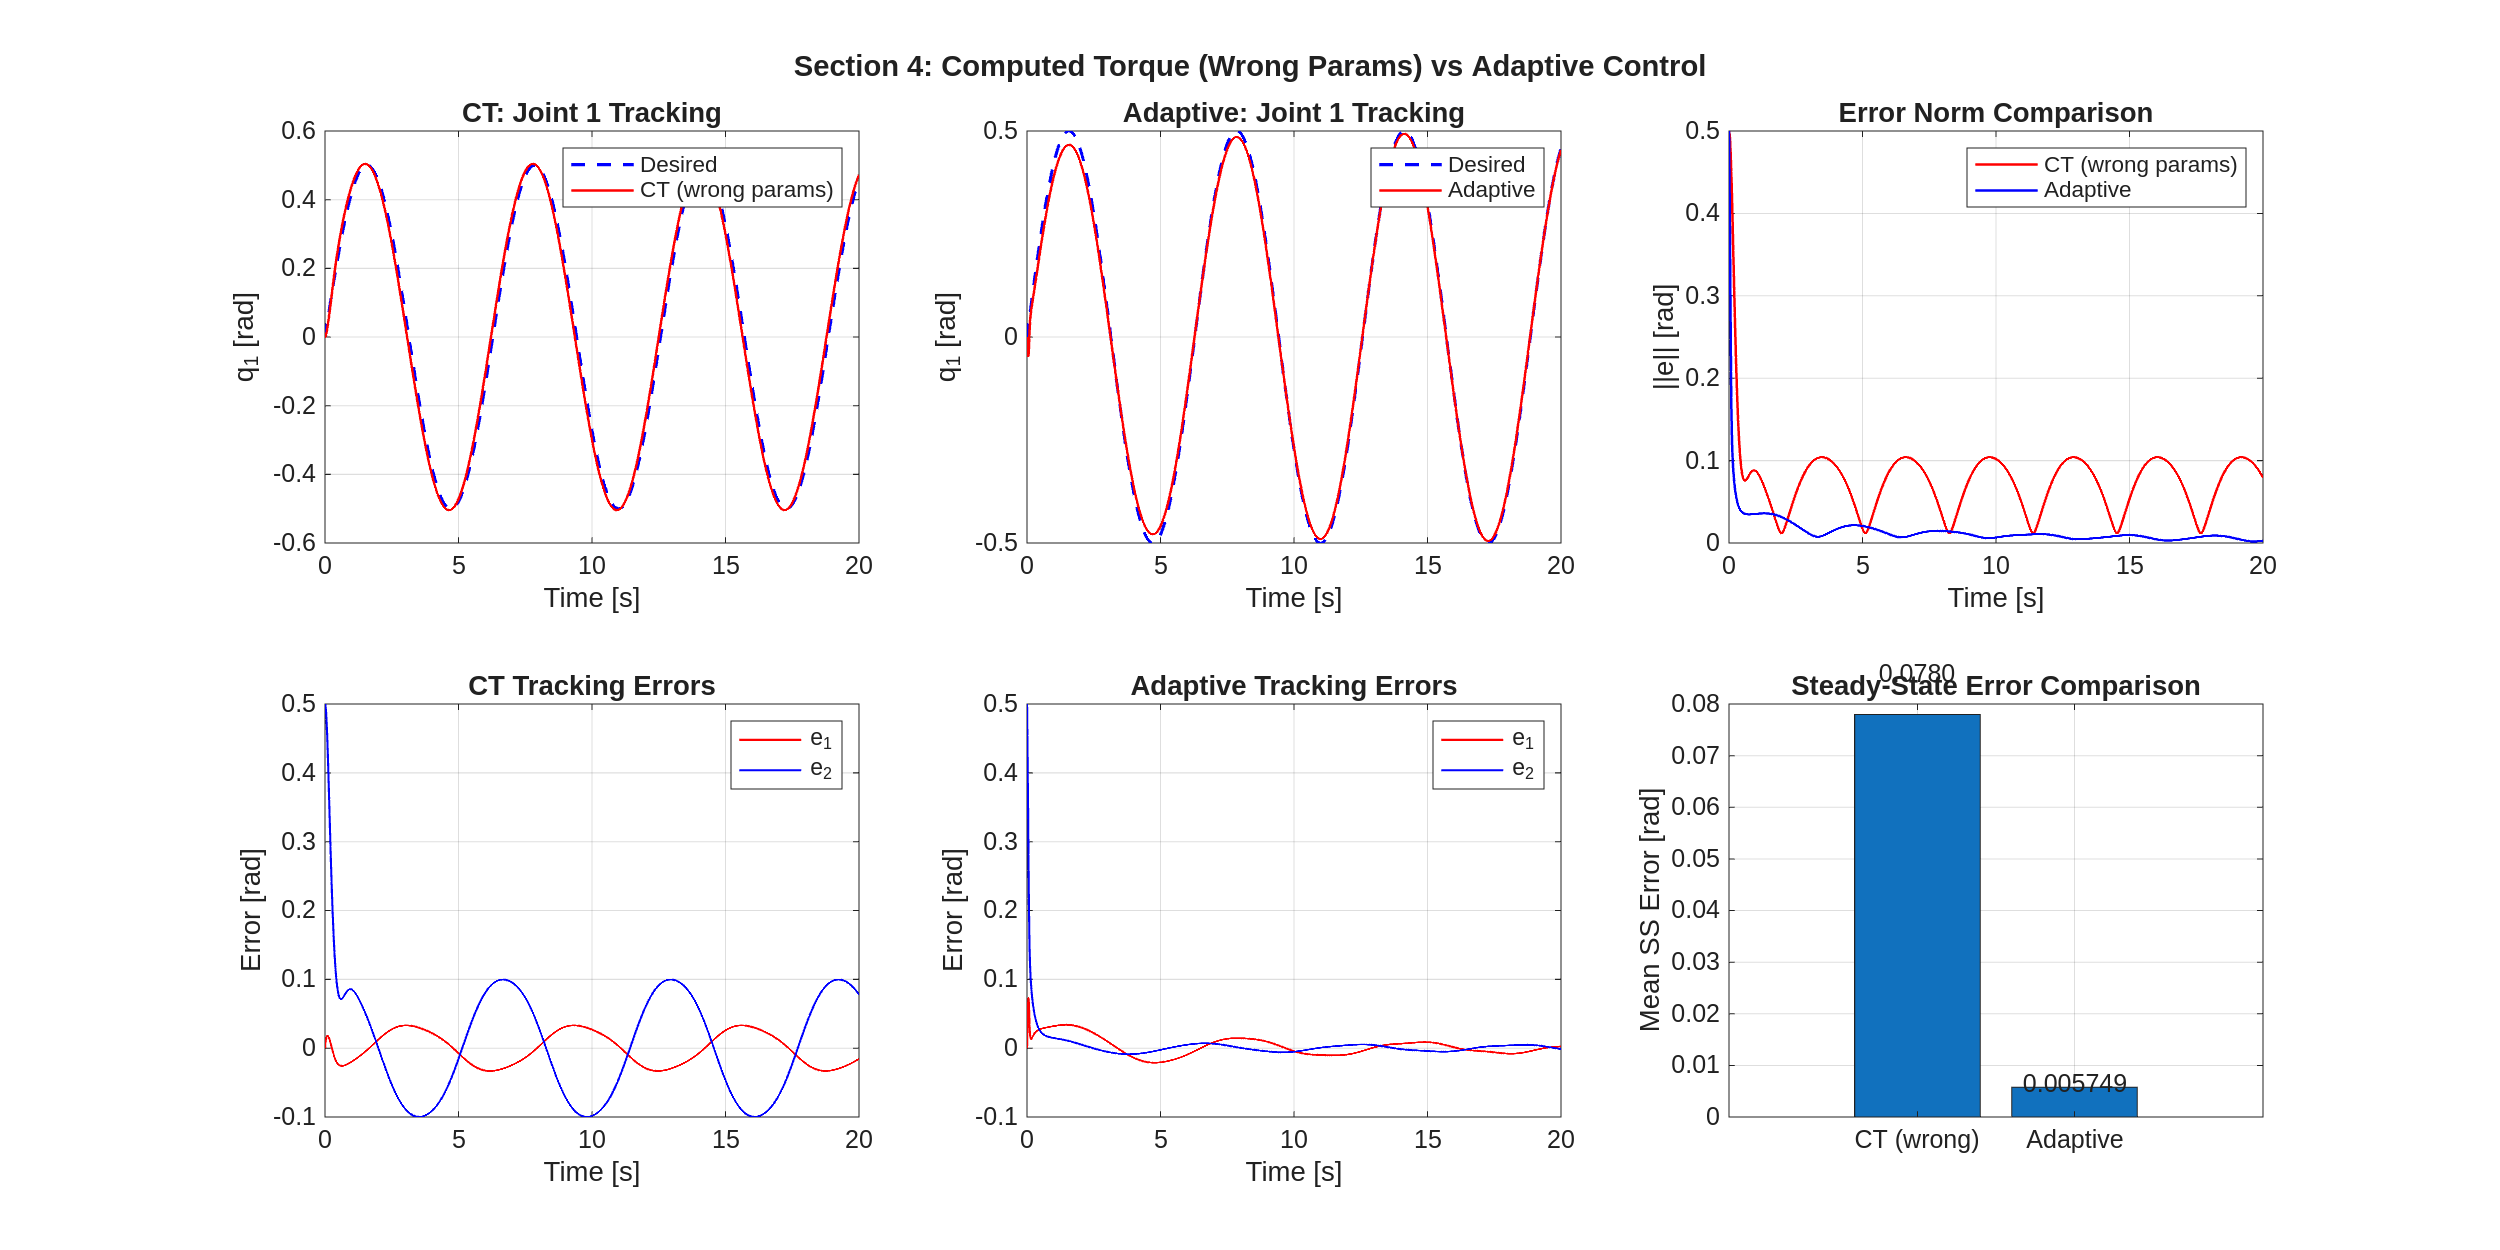
\includegraphics[width=0.92\textwidth,keepaspectratio]{images/week_04/Computed_Torque_vs_Adaptive.png}
    \caption{Computed torque vs adaptive.}
\end{figure}

\begin{figure}[ht]
    \centering
    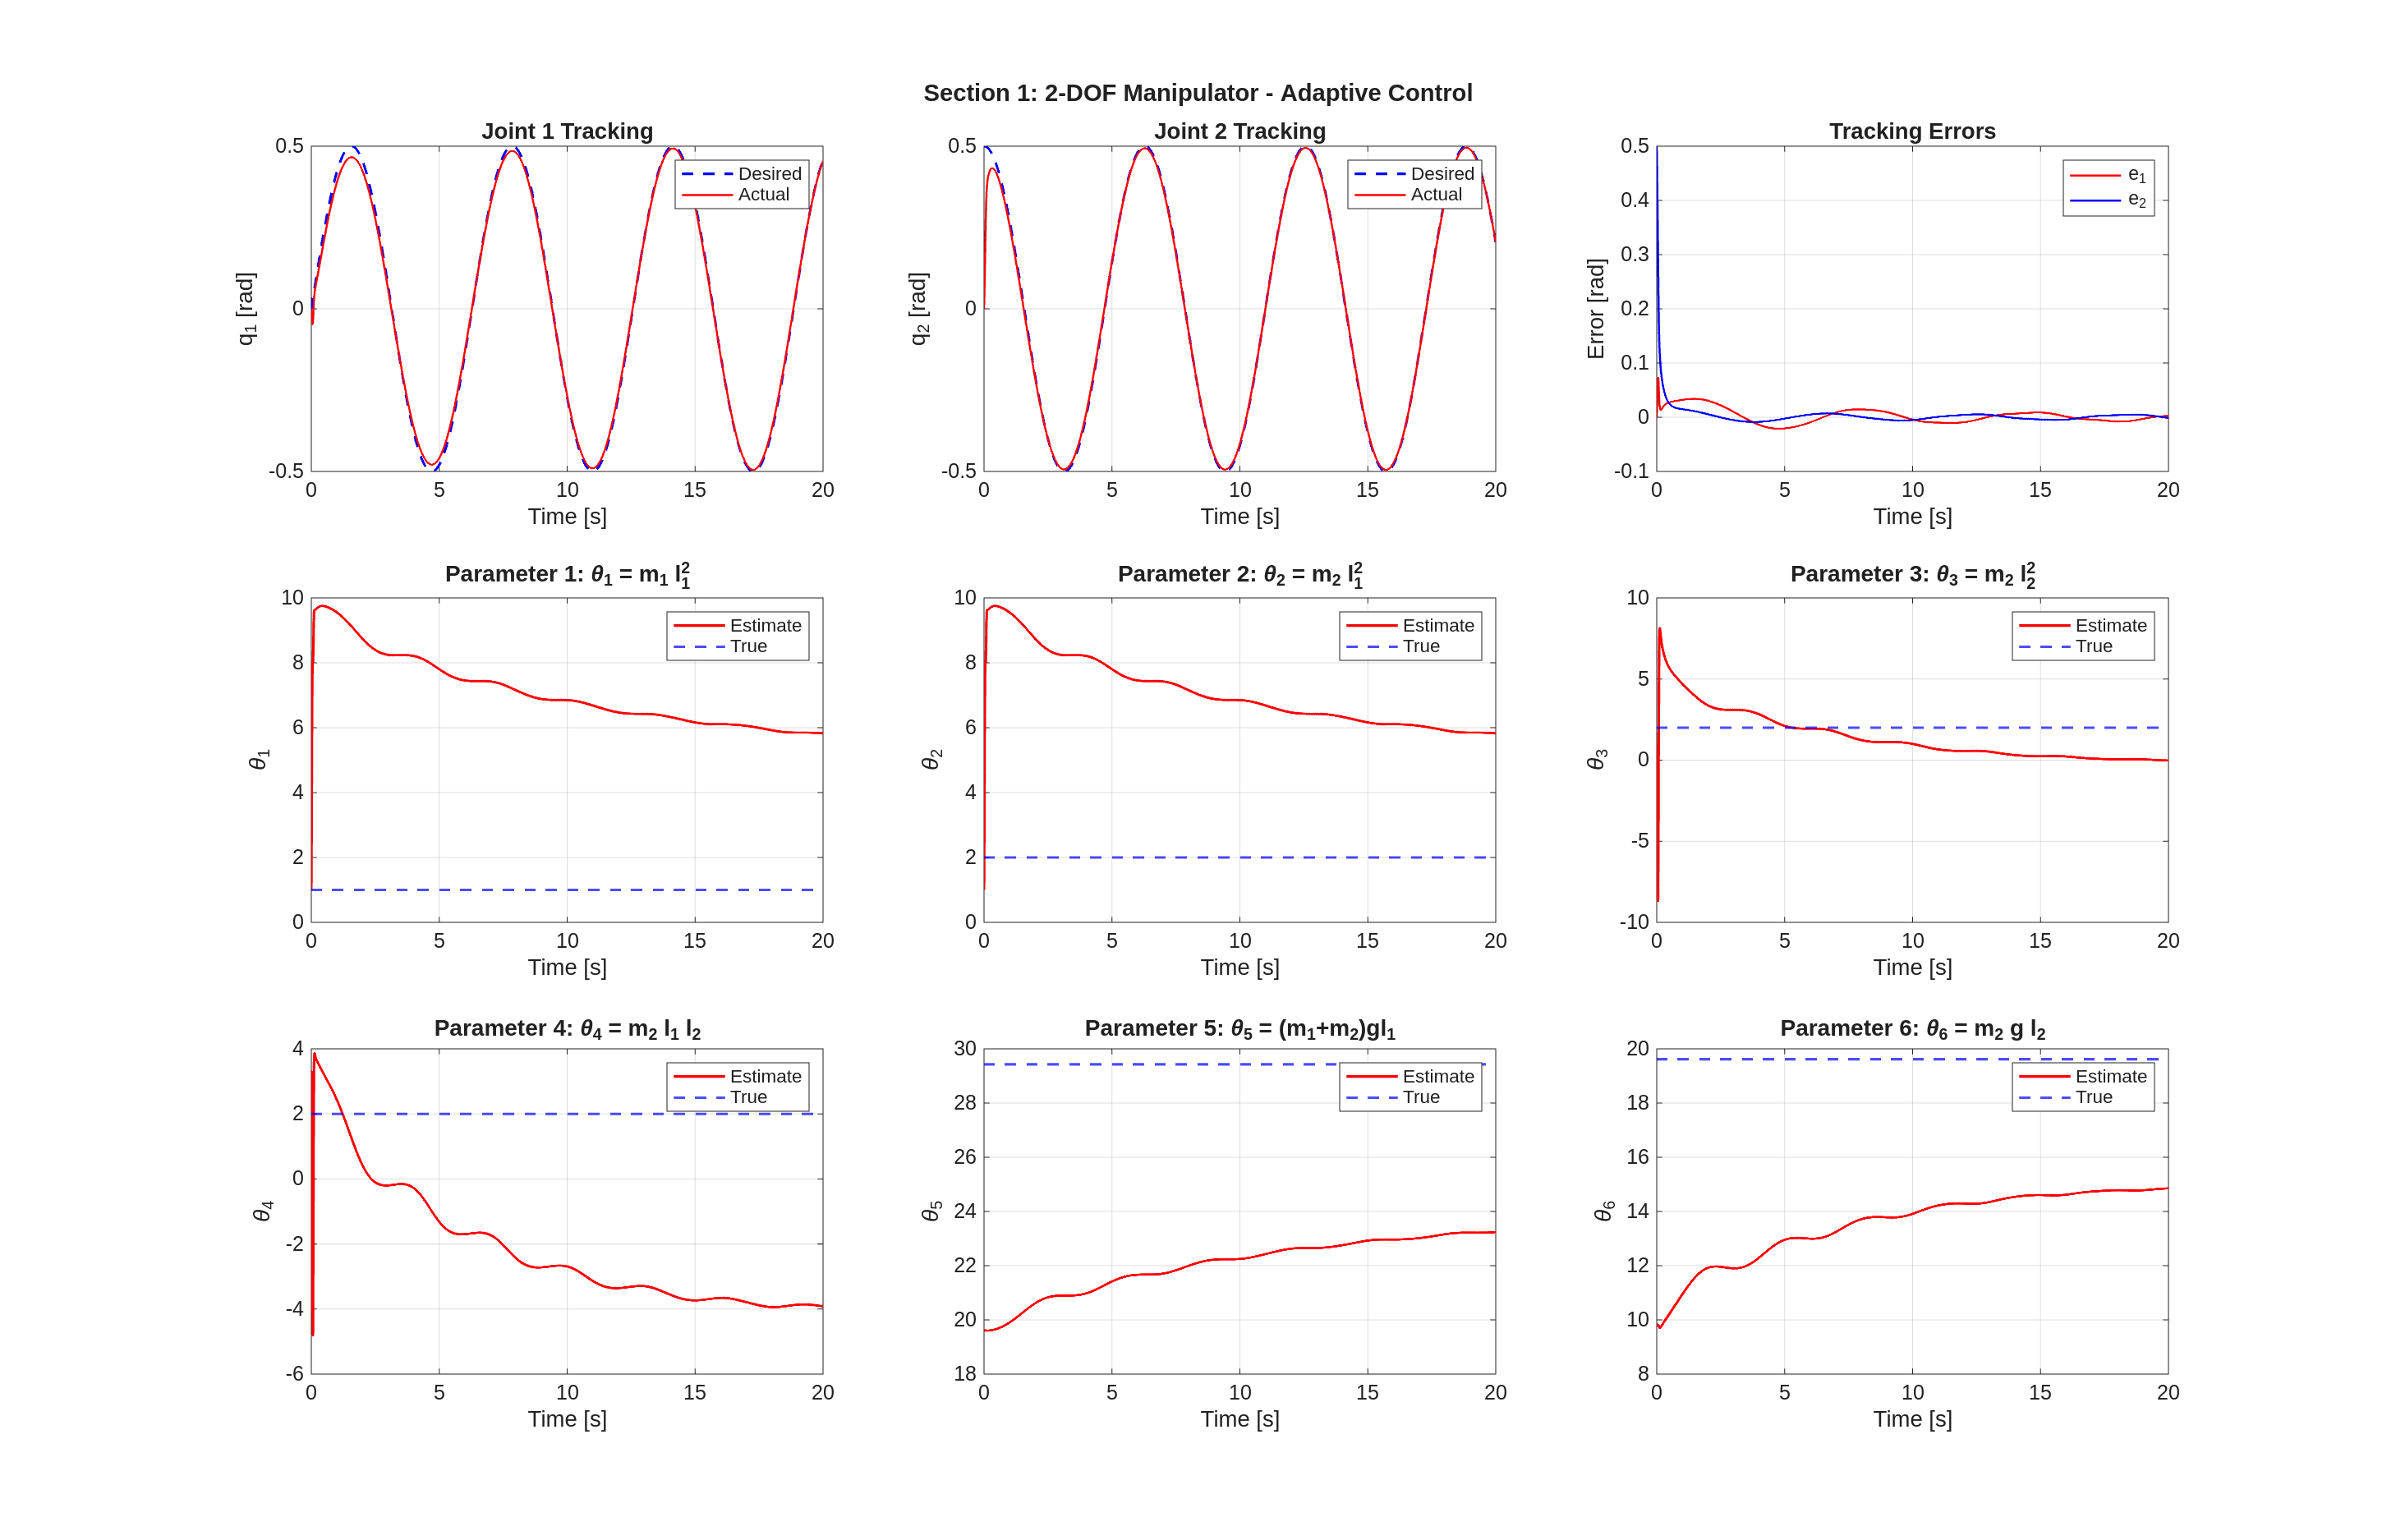
\includegraphics[width=0.92\textwidth,keepaspectratio]{images/week_04/Manipulator_Adaptive_Control.png}
    \caption{Manipulator adaptive control.}
\end{figure}

\begin{figure}[ht]
    \centering
    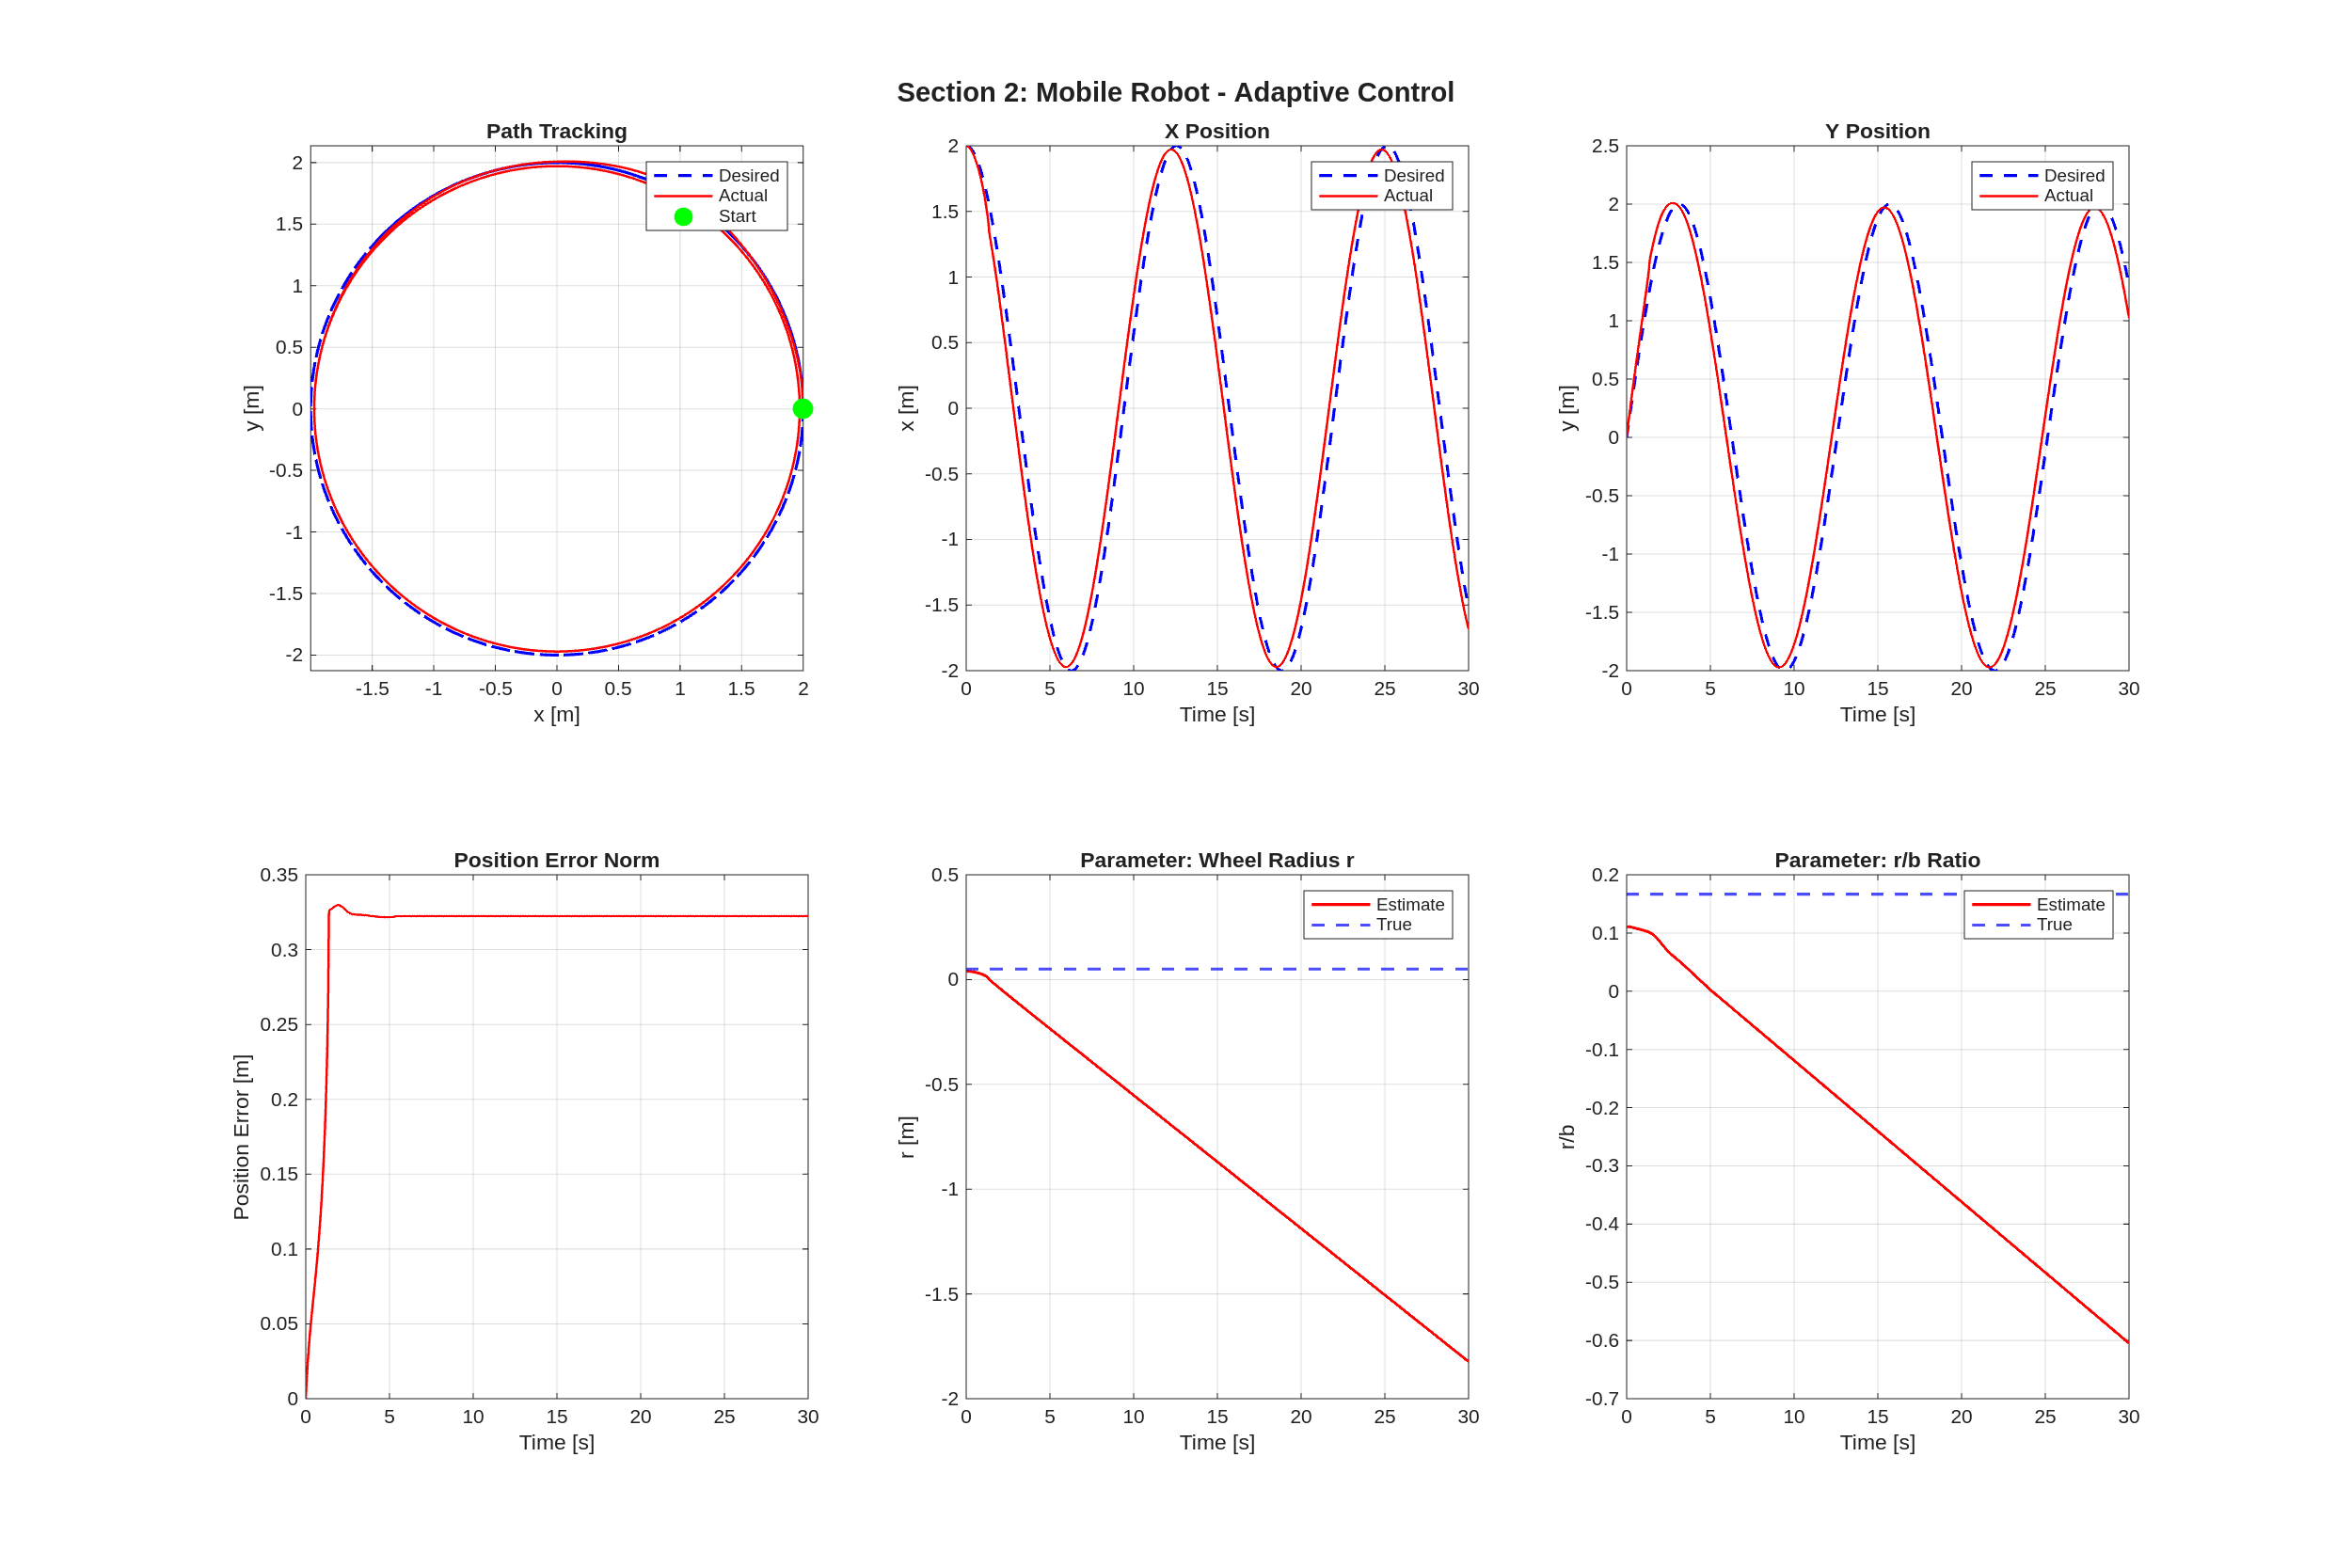
\includegraphics[width=0.92\textwidth,keepaspectratio]{images/week_04/Mobile_Robot_Adaptive_Control.png}
    \caption{Mobile robot adaptive control.}
\end{figure}

\begin{figure}[ht]
    \centering
    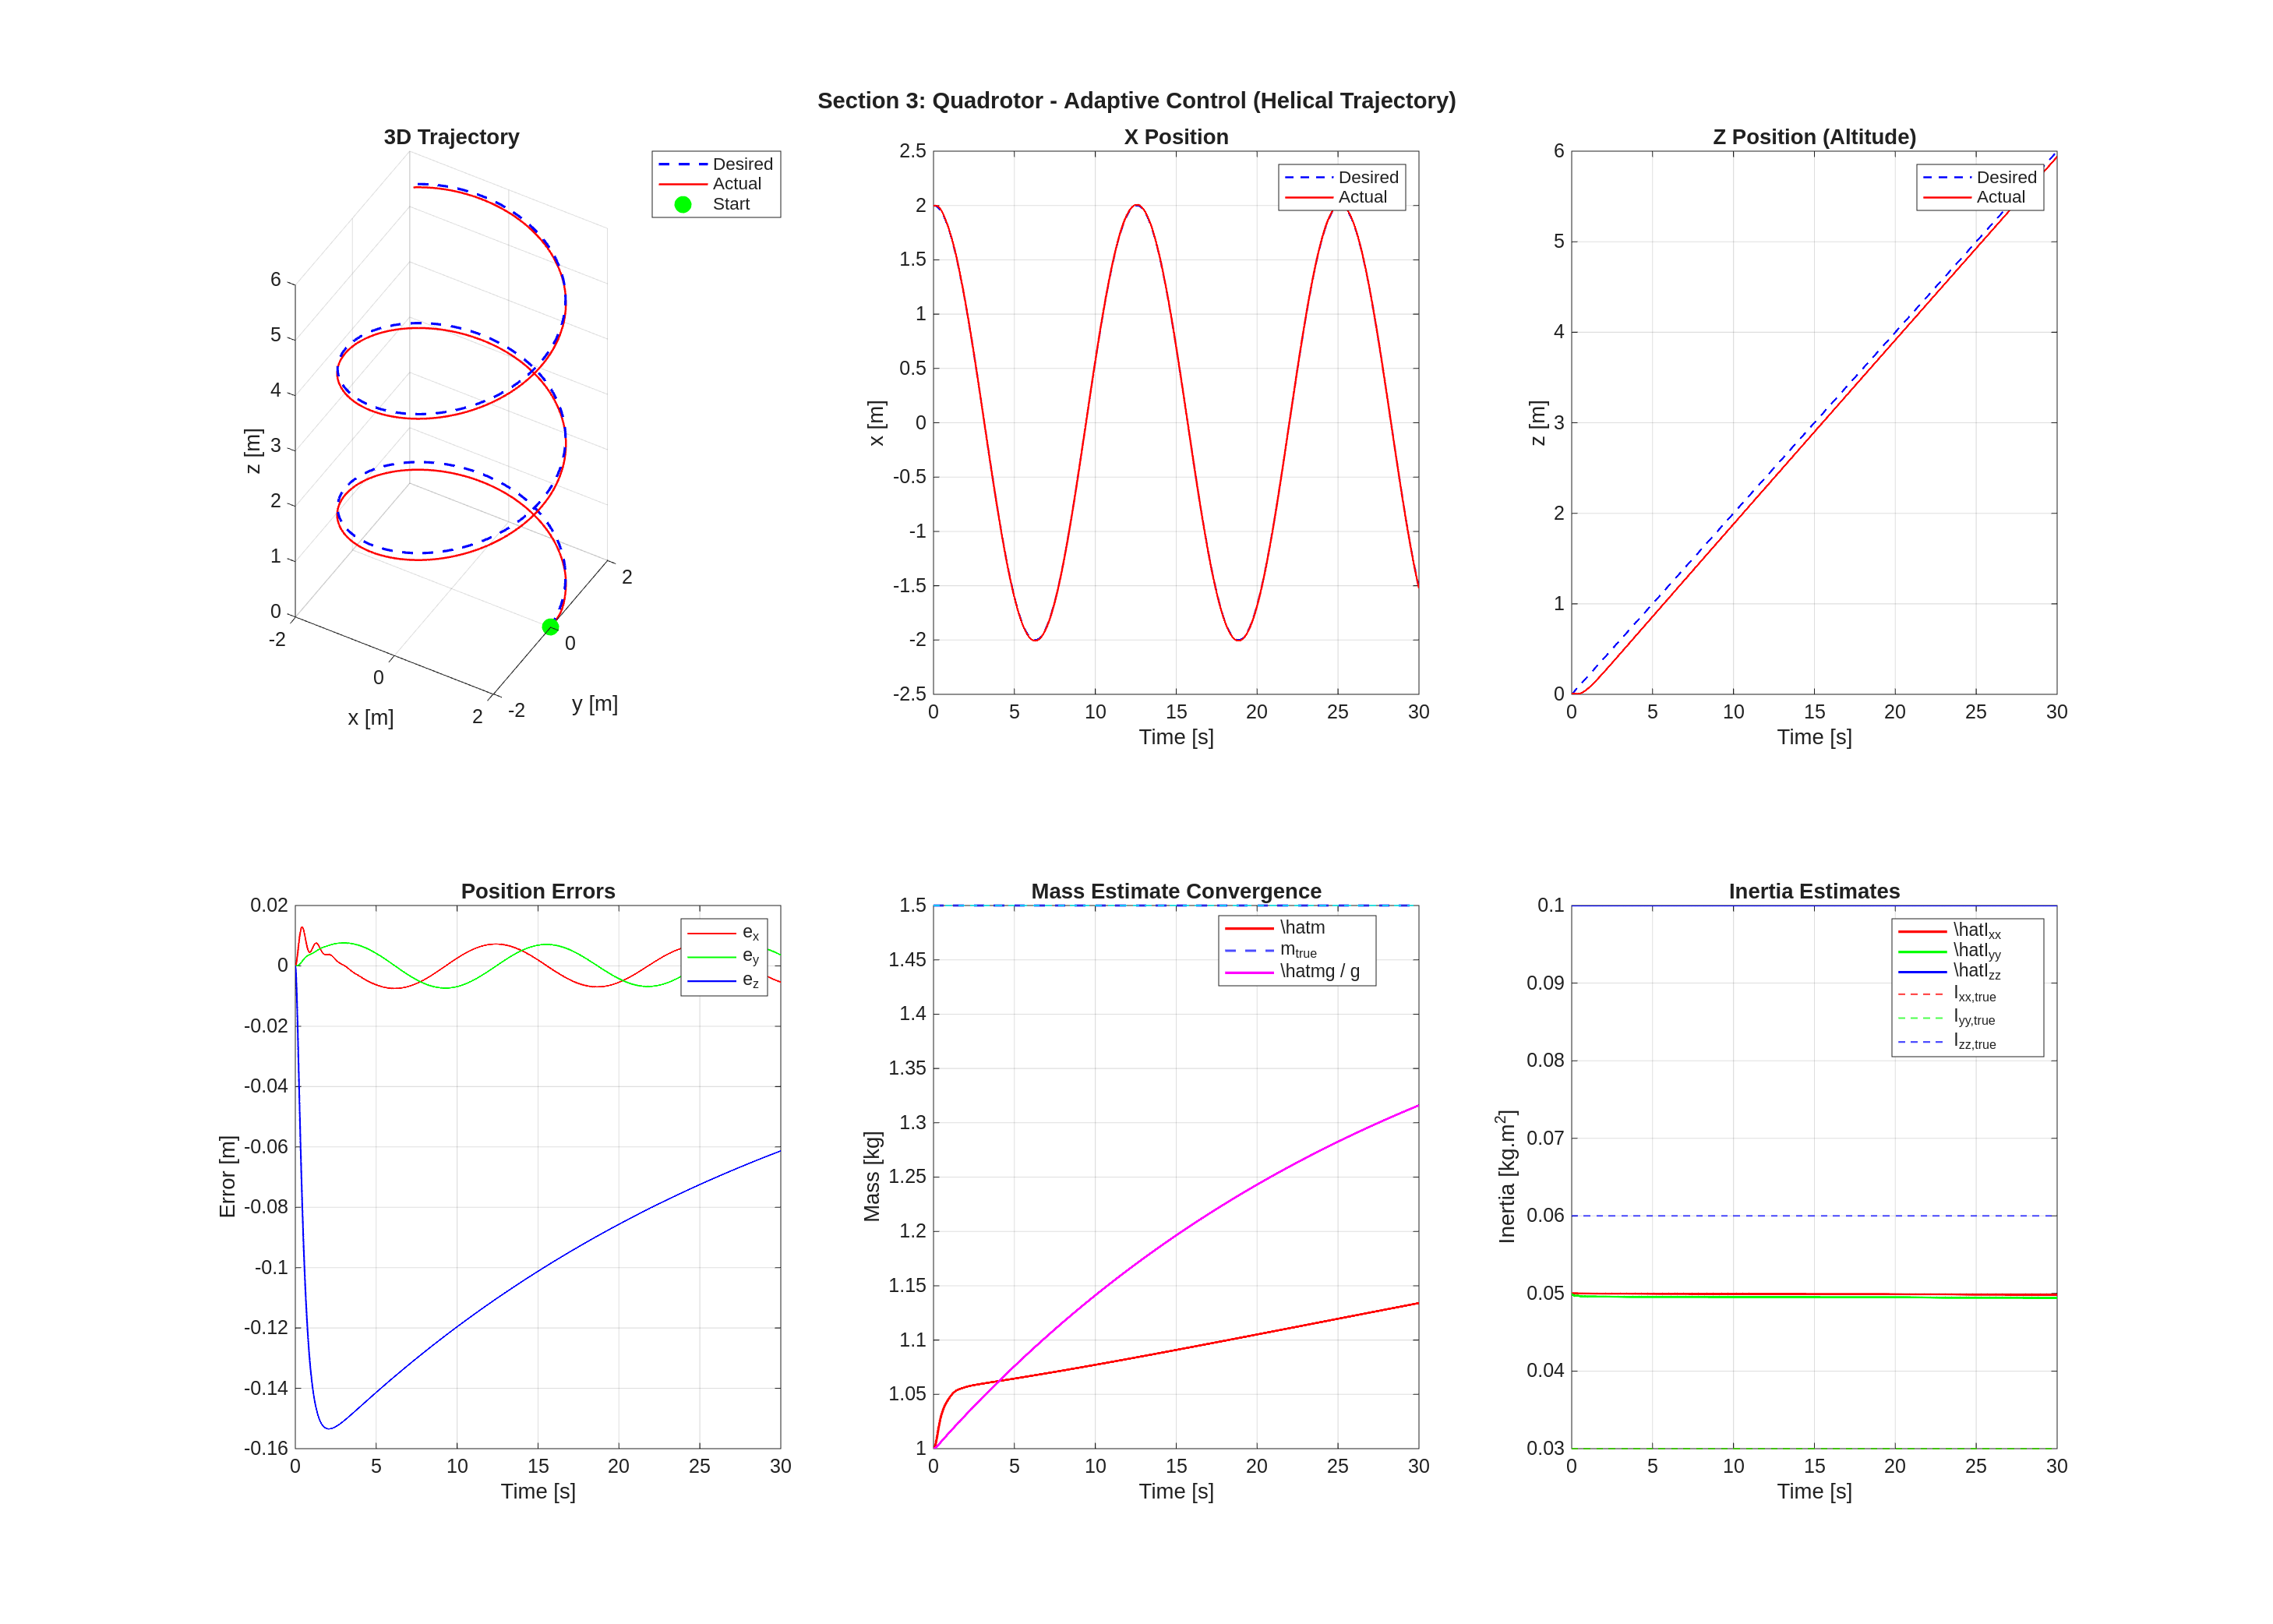
\includegraphics[width=0.92\textwidth,keepaspectratio]{images/week_04/Quadrotor_Adaptive_Control.png}
    \caption{Quadrotor adaptive control.}
\end{figure}

\section{Summary and Next Steps}

\subsection{Summary --- Control Methods Comparison}

\begin{table}[ht]\footnotesize\centering
\adjustbox{max width=\textwidth,max totalheight=0.85\textheight}{%
\begin{tabular}{llll}

\topruleProperty & Computed Torque (Week 1) & MPC (Week 2) & Adaptive Control (Week 3) \\
\midrule\bottomrule\textbf{Core idea} & Cancel nonlinearities with exact model, reduce to linear error dynamics & Predict future states over horizon, optimise control sequence online & Estimate unknown parameters online while controlling; Lyapunov guarantees stability \\
\textbf{Model requirement} & Exact knowledge of \(M(q), C(q,\dot{q}), G(q)\) & Known (possibly linearised) model for prediction & Known structure (regressor \(Y\)), unknown parameter values (\(\theta\)) \\
\textbf{Handles uncertainty?} & No --- performance degrades with parameter errors & Partially --- robust MPC variants exist but add conservatism & Yes --- explicitly designed for parametric uncertainty \\
\textbf{Handles constraints?} & No (must add saturation externally) & Yes --- naturally incorporates state and input constraints & Not directly (parameter projection can enforce bounds on \(\hat{\theta}\)) \\
\textbf{Computation} & Low --- one matrix inversion per step & High --- solves QP at each step & Low --- regressor multiply + parameter ODE integration \\
\textbf{Stability guarantee} & Exponential (with exact model) & Guaranteed with terminal cost/constraint & Asymptotic via Lyapunov + Barbalat\textquotesingle s lemma \\
\textbf{Parameter convergence} & N/A (parameters assumed known) & N/A (parameters assumed known) & Only with persistent excitation \\
\textbf{Key design parameters} & \(K_p, K_v\) (PD gains) & \(Q, R, N\) (cost weights, horizon) & \(\Lambda, K_D, \Gamma\) (sliding surface, damping, adaptation rate) \\
\textbf{Best suited for} & Well-modelled systems with known parameters & Systems with constraints, preview information, and known models & Systems with unknown or slowly-varying parameters, no constraints \\
\end{tabular}}
\end{table}


\textbf{Looking ahead --- Week 4: Robust Control.} What if the uncertainty is not parametric but includes unmodelled dynamics, disturbances, or unstructured uncertainty? Robust control (e.g., sliding mode control, \(H_\infty\)) provides guaranteed performance bounds without requiring online estimation. We will see how robust and adaptive approaches can be combined.

M.Sc. Control for Robots --- AY 2025--26

Week 3: Adaptive Control • Lecture Notes

% ----- auto-generated from week_05/Week*.html via pandoc -----
\setchapterimage[6cm]{}
\setchapterpreamble[u]{\margintoc}
\chapter{Robust Control}
\labch{week_05}

\section{Week 5: Robust Control}\label{week-5-robust-control}}

Control for Robots --- M.Sc. Robotics \& Autonomous Systems

University of West London • AY 2025--26 • 3-Hour Session

\subsection{Section 0 --- Week 4 Recall: Adaptive Control --- Exam Practice (20 min)}\label{section-0-week-4-recall-adaptive-control-exam-practice-20-min}}

\paragraph{Question 1 --- Lyapunov Stability Proof for Adaptive Control}\label{question-1-lyapunov-stability-proof-for-adaptive-control}}

Consider a 2-DOF manipulator whose dynamics are

\textbackslash{[}
M(q)\textbackslash ddot\{q\} + C(q,\textbackslash dot\{q\})\textbackslash dot\{q\} + G(q) = \textbackslash tau
\textbackslash{]}

The dynamics are \textbf{linear in parameters}:

\textbackslash{[}
M(q)\textbackslash ddot\{q\}\_r + C(q,\textbackslash dot\{q\})\textbackslash dot\{q\}\_r + G(q) = Y(q,\textbackslash dot\{q\},\textbackslash dot\{q\}\_r,\textbackslash ddot\{q\}\_r)\textbackslash,\textbackslash theta
\textbackslash{]}

where \textbackslash(\textbackslash dot\{q\}\_r = \textbackslash dot\{q\}\_d - \textbackslash Lambda e\textbackslash), \textbackslash(\textbackslash ddot\{q\}\_r = \textbackslash ddot\{q\}\_d - \textbackslash Lambda \textbackslash dot\{e\}\textbackslash), and \textbackslash(e = q - q\_d\textbackslash).

The adaptive control law is

\textbackslash{[}
\textbackslash tau = Y(q,\textbackslash dot\{q\},\textbackslash dot\{q\}\_r,\textbackslash ddot\{q\}\_r)\textbackslash,\textbackslash hat\{\textbackslash theta\} - K\_D\textbackslash,s
\textbackslash{]}

where \textbackslash(s = \textbackslash dot\{e\} + \textbackslash Lambda e = \textbackslash dot\{q\} - \textbackslash dot\{q\}\_r\textbackslash). The parameter update law is

\textbackslash{[}
\textbackslash dot\{\textbackslash hat\{\textbackslash theta\}\} = -\textbackslash Gamma\^{}\{-1\}\textbackslash,Y\^{}T s
\textbackslash{]}

\textbf{Task:} Using the Lyapunov candidate

\textbackslash{[}
V = \textbackslash tfrac\{1\}\{2\}\textbackslash,s\^{}T M(q)\textbackslash,s + \textbackslash tfrac\{1\}\{2\}\textbackslash,\textbackslash tilde\{\textbackslash theta\}\^{}T \textbackslash Gamma\textbackslash,\textbackslash tilde\{\textbackslash theta\}, \textbackslash qquad \textbackslash tilde\{\textbackslash theta\} = \textbackslash theta - \textbackslash hat\{\textbackslash theta\}
\textbackslash{]}

derive \textbackslash(\textbackslash dot\{V\}\textbackslash) step by step and show that \textbackslash(\textbackslash dot\{V\} = -s\^{}T K\_D\textbackslash,s \textbackslash le 0\textbackslash). Explain why this guarantees bounded parameter estimates.

\paragraph{Solution Outline}\label{solution-outline}}

\textbf{Step 1.} Differentiate \textbackslash(V\textbackslash):

\textbackslash{[}
\textbackslash dot\{V\} = s\^{}T M(q)\textbackslash,\textbackslash dot\{s\} + \textbackslash tfrac\{1\}\{2\}\textbackslash,s\^{}T \textbackslash dot\{M\}(q)\textbackslash,s + \textbackslash tilde\{\textbackslash theta\}\^{}T \textbackslash Gamma\textbackslash,\textbackslash dot\{\textbackslash tilde\{\textbackslash theta\}\}
\textbackslash{]}

\textbf{Step 2.} Find the closed-loop error dynamics. Substitute the control law into the manipulator equation:

\textbackslash{[}
M(q)\textbackslash dot\{s\} + C(q,\textbackslash dot\{q\})\textbackslash,s = Y\textbackslash,\textbackslash tilde\{\textbackslash theta\} - K\_D\textbackslash,s
\textbackslash{]}

This follows because \textbackslash(M\textbackslash ddot\{q\} + C\textbackslash dot\{q\} + G = \textbackslash tau\textbackslash) and \textbackslash(M\textbackslash ddot\{q\}\_r + C\textbackslash dot\{q\}\_r + G = Y\textbackslash theta\textbackslash), so subtracting gives \textbackslash(M\textbackslash dot\{s\} + Cs = Y\textbackslash theta - \textbackslash tau = Y\textbackslash theta - Y\textbackslash hat\{\textbackslash theta\} + K\_D s = Y\textbackslash tilde\{\textbackslash theta\} - K\_D s\textbackslash). Wait --- note the sign: \textbackslash(\textbackslash tau = Y\textbackslash hat\{\textbackslash theta\} - K\_D s\textbackslash), so \textbackslash(Y\textbackslash theta - \textbackslash tau = Y\textbackslash theta - Y\textbackslash hat\{\textbackslash theta\} + K\_D s = Y\textbackslash tilde\{\textbackslash theta\} + K\_D s\textbackslash). Hence:

\textbackslash{[}
M(q)\textbackslash dot\{s\} = -C(q,\textbackslash dot\{q\})\textbackslash,s + Y\textbackslash,\textbackslash tilde\{\textbackslash theta\} - K\_D\textbackslash,s
\textbackslash{]}

\textbf{Step 3.} Substitute into \textbackslash(\textbackslash dot\{V\}\textbackslash):

\textbackslash{[}
\textbackslash dot\{V\} = s\^{}T\textbackslash!\textbackslash bigl{[}-C s + Y\textbackslash tilde\{\textbackslash theta\} - K\_D s\textbackslash bigr{]} + \textbackslash tfrac\{1\}\{2\}\textbackslash,s\^{}T \textbackslash dot\{M\}\textbackslash,s + \textbackslash tilde\{\textbackslash theta\}\^{}T \textbackslash Gamma\textbackslash,\textbackslash dot\{\textbackslash tilde\{\textbackslash theta\}\}
\textbackslash{]}
\textbackslash{[}
= s\^{}T\textbackslash!\textbackslash bigl{[}\textbackslash tfrac\{1\}\{2\}(\textbackslash dot\{M\} - 2C)\textbackslash bigr{]}s + s\^{}T Y\textbackslash,\textbackslash tilde\{\textbackslash theta\} - s\^{}T K\_D\textbackslash,s + \textbackslash tilde\{\textbackslash theta\}\^{}T \textbackslash Gamma\textbackslash,\textbackslash dot\{\textbackslash tilde\{\textbackslash theta\}\}
\textbackslash{]}

\textbf{Step 4.} Use the skew-symmetry property \textbackslash(\textbackslash dot\{M\} - 2C\textbackslash) is skew-symmetric, so \textbackslash(s\^{}T(\textbackslash dot\{M\}-2C)s = 0\textbackslash):

\textbackslash{[}
\textbackslash dot\{V\} = s\^{}T Y\textbackslash,\textbackslash tilde\{\textbackslash theta\} - s\^{}T K\_D\textbackslash,s + \textbackslash tilde\{\textbackslash theta\}\^{}T \textbackslash Gamma\textbackslash,\textbackslash dot\{\textbackslash tilde\{\textbackslash theta\}\}
\textbackslash{]}

\textbf{Step 5.} Note \textbackslash(\textbackslash dot\{\textbackslash tilde\{\textbackslash theta\}\} = -\textbackslash dot\{\textbackslash hat\{\textbackslash theta\}\} = \textbackslash Gamma\^{}\{-1\} Y\^{}T s\textbackslash) (since \textbackslash(\textbackslash theta\textbackslash) is constant). Therefore:

\textbackslash{[}
\textbackslash tilde\{\textbackslash theta\}\^{}T \textbackslash Gamma\textbackslash,\textbackslash dot\{\textbackslash tilde\{\textbackslash theta\}\} = \textbackslash tilde\{\textbackslash theta\}\^{}T \textbackslash Gamma\textbackslash,\textbackslash Gamma\^{}\{-1\} Y\^{}T s = \textbackslash tilde\{\textbackslash theta\}\^{}T Y\^{}T s = (Y\textbackslash tilde\{\textbackslash theta\})\^{}T s = s\^{}T Y\textbackslash tilde\{\textbackslash theta\}
\textbackslash{]}

Wait --- this would give \textbackslash(+2s\^{}T Y\textbackslash tilde\{\textbackslash theta\}\textbackslash), which is incorrect. Let us be careful with the sign convention. We have \textbackslash(\textbackslash dot\{\textbackslash hat\{\textbackslash theta\}\} = -\textbackslash Gamma\^{}\{-1\} Y\^{}T s\textbackslash), and \textbackslash(\textbackslash tilde\{\textbackslash theta\} = \textbackslash theta - \textbackslash hat\{\textbackslash theta\}\textbackslash), so \textbackslash(\textbackslash dot\{\textbackslash tilde\{\textbackslash theta\}\} = -\textbackslash dot\{\textbackslash hat\{\textbackslash theta\}\} = \textbackslash Gamma\^{}\{-1\} Y\^{}T s\textbackslash).

Then \textbackslash(\textbackslash tilde\{\textbackslash theta\}\^{}T \textbackslash Gamma \textbackslash dot\{\textbackslash tilde\{\textbackslash theta\}\} = \textbackslash tilde\{\textbackslash theta\}\^{}T \textbackslash Gamma \textbackslash Gamma\^{}\{-1\} Y\^{}T s = \textbackslash tilde\{\textbackslash theta\}\^{}T Y\^{}T s\textbackslash). And from Step 4 we also have \textbackslash(+s\^{}T Y\textbackslash tilde\{\textbackslash theta\}\textbackslash). So we get \textbackslash(2 s\^{}T Y\textbackslash tilde\{\textbackslash theta\}\textbackslash).

The resolution: the standard adaptive law uses \textbackslash(\textbackslash dot\{\textbackslash hat\{\textbackslash theta\}\} = \textbackslash Gamma\^{}\{-1\} Y\^{}T s\textbackslash) (positive sign). Then \textbackslash(\textbackslash dot\{\textbackslash tilde\{\textbackslash theta\}\} = -\textbackslash Gamma\^{}\{-1\} Y\^{}T s\textbackslash), giving \textbackslash(\textbackslash tilde\{\textbackslash theta\}\^{}T \textbackslash Gamma \textbackslash dot\{\textbackslash tilde\{\textbackslash theta\}\} = -s\^{}T Y\textbackslash tilde\{\textbackslash theta\}\textbackslash), and the cross terms cancel:

\textbackslash{[}
\textbackslash dot\{V\} = s\^{}T Y\textbackslash tilde\{\textbackslash theta\} - s\^{}T K\_D s - s\^{}T Y\textbackslash tilde\{\textbackslash theta\} = -s\^{}T K\_D s \textbackslash le 0
\textbackslash{]}

\textbf{Step 6.} Conclusion: Since \textbackslash(V \textbackslash ge 0\textbackslash) and \textbackslash(\textbackslash dot\{V\} \textbackslash le 0\textbackslash), the function \textbackslash(V(t)\textbackslash) is non-increasing. Because \textbackslash(V\textbackslash) includes \textbackslash(\textbackslash tfrac\{1\}\{2\}\textbackslash tilde\{\textbackslash theta\}\^{}T\textbackslash Gamma\textbackslash tilde\{\textbackslash theta\}\textbackslash), boundedness of \textbackslash(V\textbackslash) implies boundedness of \textbackslash(\textbackslash tilde\{\textbackslash theta\}\textbackslash) and hence \textbackslash(\textbackslash hat\{\textbackslash theta\}\textbackslash). By Barbalat\textquotesingle s lemma, \textbackslash(s \textbackslash to 0\textbackslash) as \textbackslash(t \textbackslash to \textbackslash infty\textbackslash).

\paragraph{Question 2 --- Regressor and Parameter Vector for Gravity Terms}\label{question-2-regressor-and-parameter-vector-for-gravity-terms}}

For the same 2-DOF manipulator, the gravity vector is

\textbackslash{[}
G(q) = \textbackslash begin\{bmatrix\} (m\_1+m\_2)\textbackslash,g\textbackslash,l\_1\textbackslash cos q\_1 + m\_2\textbackslash,g\textbackslash,l\_2\textbackslash cos(q\_1+q\_2) \textbackslash\textbackslash{} m\_2\textbackslash,g\textbackslash,l\_2\textbackslash cos(q\_1+q\_2) \textbackslash end\{bmatrix\}
\textbackslash{]}

Write the regressor matrix \textbackslash(Y\_G\textbackslash) and parameter vector \textbackslash(\textbackslash theta\_G\textbackslash) such that \textbackslash(G(q) = Y\_G(q)\textbackslash,\textbackslash theta\_G\textbackslash). Identify what each element of \textbackslash(\textbackslash theta\_G\textbackslash) represents physically.

\paragraph{Solution}\label{solution}}

We seek a factorisation \textbackslash(G(q) = Y\_G(q)\textbackslash,\textbackslash theta\_G\textbackslash). Observe that the gravity terms depend on two independent parameter groups:

\begin{itemize}
\tightlist
\item
  \textbackslash(\textbackslash theta\_\{G,1\} = (m\_1 + m\_2)\textbackslash,g\textbackslash,l\_1\textbackslash) --- gravitational torque parameter for link 1 (total mass times gravity times link-1 length)
\item
  \textbackslash(\textbackslash theta\_\{G,2\} = m\_2\textbackslash,g\textbackslash,l\_2\textbackslash) --- gravitational torque parameter for link 2 (link-2 mass times gravity times link-2 length)
\end{itemize}

Then:

\textbackslash{[}
G(q) = \textbackslash underbrace\{\textbackslash begin\{bmatrix\} \textbackslash cos q\_1 \& \textbackslash cos(q\_1+q\_2) \textbackslash\textbackslash{} 0 \& \textbackslash cos(q\_1+q\_2) \textbackslash end\{bmatrix\}\}\_\{Y\_G(q)\} \textbackslash underbrace\{\textbackslash begin\{bmatrix\} (m\_1+m\_2)\textbackslash,g\textbackslash,l\_1 \textbackslash\textbackslash{} m\_2\textbackslash,g\textbackslash,l\_2 \textbackslash end\{bmatrix\}\}\_\{\textbackslash theta\_G\}
\textbackslash{]}

\textbf{Physical meaning:}

\begin{itemize}
\tightlist
\item
  \textbackslash(\textbackslash theta\_\{G,1\} = (m\_1+m\_2)gl\_1\textbackslash): the maximum gravitational torque that link 1 must support (both link masses hanging at full link-1 lever arm).
\item
  \textbackslash(\textbackslash theta\_\{G,2\} = m\_2 g l\_2\textbackslash): the maximum gravitational torque due to link 2 alone (link-2 mass at full link-2 lever arm).
\end{itemize}

\textbf{Time Limit:} 20 minutes to complete both questions. Work individually first, then discuss with your neighbour.

\subsection{Section 1 --- Learning Outcomes}\label{section-1-learning-outcomes}}

\begin{itemize}
\tightlist
\item
  Understand robust control philosophy: guarantee performance despite \textbf{bounded} uncertainties without estimating them
\item
  Derive a robust control law for a manipulator subject to bounded disturbances
\item
  Understand \textbackslash(\textbackslash mathcal\{H\}\_\textbackslash infty\textbackslash) control concepts and their application to robotics
\item
  Apply robust PD+ control with known disturbance bounds
\item
  Implement robust control for three systems: manipulator, mobile robot, drone
\item
  Compare robust control vs adaptive control vs computed torque control
\end{itemize}

\subsection{Section 2 --- Session Roadmap (3 Hours)}\label{section-2-session-roadmap-3-hours}}

0:00 -- 0:20

\paragraph{Previous Week Exam Practice}\label{previous-week-exam-practice}}

Adaptive control recall: Lyapunov proof and regressor identification.

0:20 -- 1:00

\paragraph{Part 1 --- Robust Control Theory}\label{part-1-robust-control-theory}}

Philosophy, problem setup, robust term design, Lyapunov proof, \textbackslash(\textbackslash mathcal\{H\}\_\textbackslash infty\textbackslash) concepts.

1:00 -- 1:20

\paragraph{Part 2 --- Robust Control for Manipulator}\label{part-2-robust-control-for-manipulator}}

Full derivation for 2-DOF arm, uncertainty bounds, MATLAB implementation.

1:20 -- 1:30

\paragraph{Break}\label{break}}

10-minute break.

1:30 -- 2:00

\paragraph{Part 3 --- Robust Control for Mobile Robot}\label{part-3-robust-control-for-mobile-robot}}

Wheel slip, terrain disturbances, robust unicycle tracking.

2:00 -- 2:30

\paragraph{Part 4 --- Robust Control for Drone}\label{part-4-robust-control-for-drone}}

Wind disturbance rejection, robust position and attitude control.

2:30 -- 3:00

\paragraph{Part 5 --- MATLAB \& Activities}\label{part-5-matlab-activities}}

Hands-on simulation, comparison exercises, quick quiz.

\subsection{Section 3 --- Part 1: Robust Control Theory}\label{section-3-part-1-robust-control-theory}}

\subsubsection{3.1 Why Robust Control?}\label{why-robust-control}}

In Weeks 1--3 we developed increasingly sophisticated controllers:

\begin{itemize}
\tightlist
\item
  \textbf{Computed Torque (Week 1):} requires exact model --- any mismatch degrades performance.
\item
  \textbf{MPC (Week 2):} optimises over a prediction horizon using a model --- sensitive to model error.
\item
  \textbf{Adaptive Control (Week 3):} estimates unknown parameters online --- but requires linearity in parameters and persistent excitation.
\end{itemize}

\textbf{Robust control} takes a different philosophy:

\textbf{Core Idea:} Instead of estimating the uncertainty, assume it is \emph{bounded} and design a controller that guarantees performance for \emph{all} disturbances within that bound. No online estimation, no model identification --- just guaranteed worst-case performance.

\textbf{Figure 1:} Robust control block diagram showing the nominal plant with additive uncertainty block Δ and disturbance d(t). The robust controller compensates for all bounded uncertainties without estimating them.

\paragraph{When to Use Robust Control}\label{when-to-use-robust-control}}

\begin{itemize}
\tightlist
\item
  Uncertainty bound is known (e.g., wind ≤ 10 N)
\item
  Parameters change too fast for adaptation
\item
  Safety-critical: need guaranteed bounds on tracking error
\item
  Simple implementation desired (no online estimation)
\end{itemize}

\paragraph{When NOT to Use Robust Control}\label{when-not-to-use-robust-control}}

\begin{itemize}
\tightlist
\item
  Uncertainty bound is unknown or very conservative
\item
  Performance must improve over time (use adaptive)
\item
  Large parametric uncertainty (robust term becomes too large)
\item
  Tight energy constraints (robust terms use more control effort)
\end{itemize}

\subsubsection{3.2 Problem Setup}\label{problem-setup}}

Consider the general manipulator dynamics with a \textbf{bounded disturbance}:

\textbackslash{[}
M(q)\textbackslash,\textbackslash ddot\{q\} + C(q,\textbackslash dot\{q\})\textbackslash,\textbackslash dot\{q\} + G(q) = \textbackslash tau + d(t), \textbackslash qquad \textbackslash\textbar d(t)\textbackslash\textbar{} \textbackslash le d\_\{\textbackslash max\}
\textbackslash{]}

Here \textbackslash(d(t) \textbackslash in \textbackslash mathbb\{R\}\^{}n\textbackslash) represents \emph{all} unmodelled effects: external forces, friction, payload changes, model mismatch, sensor noise coupling, etc. The only assumption is a known upper bound \textbackslash(d\_\{\textbackslash max\}\textbackslash).

Additionally, suppose we have an \textbf{imperfect model}: estimates \textbackslash(\textbackslash hat\{M\}(q)\textbackslash), \textbackslash(\textbackslash hat\{C\}(q,\textbackslash dot\{q\})\textbackslash), \textbackslash(\textbackslash hat\{G\}(q)\textbackslash) with bounded errors:

\textbackslash{[}
\textbackslash Delta M = M - \textbackslash hat\{M\}, \textbackslash quad \textbackslash Delta C = C - \textbackslash hat\{C\}, \textbackslash quad \textbackslash Delta G = G - \textbackslash hat\{G\}
\textbackslash{]}

Then the total uncertainty is:

\textbackslash{[}
\textbackslash eta(t) = \textbackslash Delta M\textbackslash,\textbackslash ddot\{q\} + \textbackslash Delta C\textbackslash,\textbackslash dot\{q\} + \textbackslash Delta G + d(t)
\textbackslash{]}

If we can bound \textbackslash(\textbackslash\textbar\textbackslash eta(t)\textbackslash\textbar{} \textbackslash le \textbackslash rho(q,\textbackslash dot\{q\},t)\textbackslash) for a known function \textbackslash(\textbackslash rho\textbackslash), we can design a robust controller.

\textbf{Figure 2:} Three types of uncertainty: (a) parametric -\/- parameters lie in known intervals; (b) unstructured/additive -\/- frequency-dependent uncertainty envelope around the nominal response; (c) matched disturbance -\/- bounded signal entering at the plant input.

\subsubsection{3.3 Robust Computed Torque + Robust Term}\label{robust-computed-torque-robust-term}}

The control law has two components:

\textbackslash{[}
\textbackslash tau = \textbackslash underbrace\{\textbackslash hat\{M\}(q)\textbackslash bigl{[}\textbackslash ddot\{q\}\_d + K\_D\textbackslash,\textbackslash dot\{e\} + K\_P\textbackslash,e\textbackslash bigr{]} + \textbackslash hat\{C\}(q,\textbackslash dot\{q\})\textbackslash,\textbackslash dot\{q\} + \textbackslash hat\{G\}(q)\}\_\{\textbackslash text\{nominal computed torque\}\} + \textbackslash underbrace\{\textbackslash tau\_\{\textbackslash text\{robust\}\}\}\_\{\textbackslash text\{robust term\}\}
\textbackslash{]}

where \textbackslash(e = q\_d - q\textbackslash) is the tracking error.

\paragraph{Closed-Loop Error Dynamics}\label{closed-loop-error-dynamics}}

Substituting into the manipulator equation:

\textbackslash{[}
M\textbackslash ddot\{q\} + C\textbackslash dot\{q\} + G = \textbackslash hat\{M\}(\textbackslash ddot\{q\}\_d + K\_D\textbackslash dot\{e\} + K\_P e) + \textbackslash hat\{C\}\textbackslash dot\{q\} + \textbackslash hat\{G\} + \textbackslash tau\_\{\textbackslash text\{robust\}\} + d
\textbackslash{]}

Rearranging with \textbackslash(\textbackslash ddot\{e\} = \textbackslash ddot\{q\}\_d - \textbackslash ddot\{q\}\textbackslash):

\textbackslash{[}
M\textbackslash ddot\{e\} + (C + \textbackslash hat\{M\}K\_D)\textbackslash dot\{e\} + \textbackslash hat\{M\}K\_P e = \textbackslash underbrace\{\textbackslash Delta M\textbackslash ddot\{q\} + \textbackslash Delta C\textbackslash dot\{q\} + \textbackslash Delta G + d(t)\}\_\{\textbackslash eta(t)\} - \textbackslash tau\_\{\textbackslash text\{robust\}\}
\textbackslash{]}

\subsubsection{3.4 Robust Term Design}\label{robust-term-design}}

Define the \textbf{sliding variable} (same as in adaptive control):

\textbackslash{[}
s = \textbackslash dot\{e\} + \textbackslash Lambda\textbackslash,e
\textbackslash{]}

where \textbackslash(\textbackslash Lambda \textbackslash succ 0\textbackslash) is a positive-definite gain matrix. Then the robust controller is:

\textbackslash{[}
\textbackslash tau = \textbackslash hat\{M\}(q)\textbackslash,\textbackslash ddot\{q\}\_r + \textbackslash hat\{C\}(q,\textbackslash dot\{q\})\textbackslash,\textbackslash dot\{q\}\_r + \textbackslash hat\{G\}(q) - K\_D\textbackslash,s + \textbackslash tau\_\{\textbackslash text\{robust\}\}
\textbackslash{]}

where \textbackslash(\textbackslash dot\{q\}\_r = \textbackslash dot\{q\}\_d - \textbackslash Lambda e\textbackslash), \textbackslash(\textbackslash ddot\{q\}\_r = \textbackslash ddot\{q\}\_d - \textbackslash Lambda\textbackslash dot\{e\}\textbackslash) (the reference velocity and acceleration).

The \textbf{robust term} is designed as:

\textbackslash{[}
\textbackslash tau\_\{\textbackslash text\{robust\}\} = \textbackslash begin\{cases\} -\textbackslash rho(t)\textbackslash,\textbackslash dfrac\{s\}\{\textbackslash\textbar s\textbackslash\textbar\} \& \textbackslash text\{if \} \textbackslash\textbar s\textbackslash\textbar{} \textbackslash ge \textbackslash epsilon \textbackslash\textbackslash{} -\textbackslash dfrac\{\textbackslash rho(t)\}\{\textbackslash epsilon\}\textbackslash,s \& \textbackslash text\{if \} \textbackslash\textbar s\textbackslash\textbar{} \textless{} \textbackslash epsilon \textbackslash end\{cases\}
\textbackslash{]}

where \textbackslash(\textbackslash rho(t) \textbackslash ge \textbackslash\textbar\textbackslash eta(t)\textbackslash\textbar\textbackslash) is the uncertainty bound and \textbackslash(\textbackslash epsilon \textgreater{} 0\textbackslash) is a small boundary-layer thickness to avoid chattering. The first case is the \textbf{discontinuous} (sliding-mode-like) form; the second is a \textbf{continuous approximation} inside a boundary layer.

\textbf{Chattering Problem:} The pure discontinuous form \textbackslash(\textbackslash tau\_\{\textbackslash text\{robust\}\} = -\textbackslash rho\textbackslash,s/\textbackslash\textbar s\textbackslash\textbar\textbackslash) causes high-frequency switching (chattering) in actuators. The boundary layer \textbackslash(\textbackslash epsilon\textbackslash) trades off robustness for smoothness. Smaller \textbackslash(\textbackslash epsilon\textbackslash) = more robust but more chattering.

\subsubsection{3.5 Lyapunov Stability Proof}\label{lyapunov-stability-proof}}

\paragraph{Theorem: Robust Tracking with Bounded Error}\label{theorem-robust-tracking-with-bounded-error}}

Consider the Lyapunov candidate:

\textbackslash{[}
V = \textbackslash tfrac\{1\}\{2\}\textbackslash,s\^{}T M(q)\textbackslash,s
\textbackslash{]}

\textbf{Step 1.} Differentiate:

\textbackslash{[}
\textbackslash dot\{V\} = s\^{}T M\textbackslash dot\{s\} + \textbackslash tfrac\{1\}\{2\}s\^{}T\textbackslash dot\{M\}s
\textbackslash{]}

\textbf{Step 2.} The closed-loop error dynamics give:

\textbackslash{[}
M\textbackslash dot\{s\} = -Cs + \textbackslash eta(t) - K\_D s + \textbackslash tau\_\{\textbackslash text\{robust\}\}
\textbackslash{]}

Substituting:

\textbackslash{[}
\textbackslash dot\{V\} = s\^{}T(-Cs + \textbackslash eta - K\_D s + \textbackslash tau\_\{\textbackslash text\{robust\}\}) + \textbackslash tfrac\{1\}\{2\}s\^{}T\textbackslash dot\{M\}s
\textbackslash{]}
\textbackslash{[}
= \textbackslash tfrac\{1\}\{2\}s\^{}T(\textbackslash dot\{M\}-2C)s + s\^{}T\textbackslash eta - s\^{}T K\_D s + s\^{}T\textbackslash tau\_\{\textbackslash text\{robust\}\}
\textbackslash{]}

\textbf{Step 3.} By skew-symmetry, \textbackslash(s\^{}T(\textbackslash dot\{M\}-2C)s = 0\textbackslash):

\textbackslash{[}
\textbackslash dot\{V\} = s\^{}T\textbackslash eta - s\^{}T K\_D s + s\^{}T\textbackslash tau\_\{\textbackslash text\{robust\}\}
\textbackslash{]}

\textbf{Step 4.} For the discontinuous case (\textbackslash(\textbackslash\textbar s\textbackslash\textbar{} \textbackslash ge \textbackslash epsilon\textbackslash)), \textbackslash(\textbackslash tau\_\{\textbackslash text\{robust\}\} = -\textbackslash rho\textbackslash,s/\textbackslash\textbar s\textbackslash\textbar\textbackslash):

\textbackslash{[}
s\^{}T\textbackslash tau\_\{\textbackslash text\{robust\}\} = -\textbackslash rho\textbackslash,\textbackslash frac\{s\^{}Ts\}\{\textbackslash\textbar s\textbackslash\textbar\} = -\textbackslash rho\textbackslash,\textbackslash\textbar s\textbackslash\textbar{}
\textbackslash{]}

And \textbackslash(s\^{}T\textbackslash eta \textbackslash le \textbackslash\textbar s\textbackslash\textbar\textbackslash,\textbackslash\textbar\textbackslash eta\textbackslash\textbar{} \textbackslash le \textbackslash\textbar s\textbackslash\textbar\textbackslash,\textbackslash rho\textbackslash) by Cauchy--Schwarz and the bound \textbackslash(\textbackslash\textbar\textbackslash eta\textbackslash\textbar{} \textbackslash le \textbackslash rho\textbackslash). Therefore:

\textbackslash{[}
\textbackslash dot\{V\} \textbackslash le \textbackslash\textbar s\textbackslash\textbar\textbackslash rho - s\^{}T K\_D s - \textbackslash rho\textbackslash\textbar s\textbackslash\textbar{} = -s\^{}T K\_D s \textbackslash le 0
\textbackslash{]}

\textbf{Step 5.} For the boundary-layer case (\textbackslash(\textbackslash\textbar s\textbackslash\textbar{} \textless{} \textbackslash epsilon\textbackslash)), the tracking error is already within the boundary layer. The ultimate bound on \textbackslash(\textbackslash\textbar s\textbackslash\textbar\textbackslash) is \textbackslash(\textbackslash epsilon\textbackslash), which translates to a bounded tracking error.

\textbf{Result:} With the robust term, the sliding variable \textbackslash(s\textbackslash) converges to the boundary layer \textbackslash(\textbackslash\textbar s\textbackslash\textbar{} \textbackslash le \textbackslash epsilon\textbackslash), guaranteeing that tracking error is ultimately bounded. With \textbackslash(s = \textbackslash dot\{e\}+\textbackslash Lambda e \textbackslash to 0\textbackslash), we get \textbackslash(e \textbackslash to 0\textbackslash) exponentially inside the boundary layer.

\textbf{Figure 4:} Robust stability comparison. Left: nominal system without disturbance -\/- the trajectory converges asymptotically to the origin along Lyapunov contours. Right: robust system with bounded disturbance -\/- the trajectory converges to a bounded ball of radius ε (the ultimate bound), which depends on the boundary layer thickness and gains.

\subsubsection{3.6 \textbackslash(\textbackslash mathcal\{H\}\_\textbackslash infty\textbackslash) Control Concepts}\label{mathcalh_infty-control-concepts}}

\textbackslash(\textbackslash mathcal\{H\}\_\textbackslash infty\textbackslash) (H-infinity) control is the \textbf{frequency-domain} counterpart to the Lyapunov-based robust control above. The key idea:

\textbf{Goal:} Design a controller \textbackslash(K\textbackslash) that minimises the worst-case gain from disturbance \textbackslash(w\textbackslash) to performance output \textbackslash(z\textbackslash):
\textbackslash{[}
\textbackslash min\_K \textbackslash;\textbackslash\textbar T\_\{zw\}(s)\textbackslash\textbar\_\textbackslash infty = \textbackslash min\_K \textbackslash;\textbackslash sup\_\textbackslash omega \textbackslash;\textbackslash bar\{\textbackslash sigma\}\textbackslash!\textbackslash bigl(T\_\{zw\}(j\textbackslash omega)\textbackslash bigr)
\textbackslash{]}
where \textbackslash(\textbackslash bar\{\textbackslash sigma\}\textbackslash) is the maximum singular value.

\paragraph{Standard Plant Formulation}\label{standard-plant-formulation}}

The generalised plant \textbackslash(P\textbackslash) connects disturbance \textbackslash(w\textbackslash), control \textbackslash(u\textbackslash), performance output \textbackslash(z\textbackslash), and measurement \textbackslash(y\textbackslash):

\textbackslash{[}
\textbackslash begin\{bmatrix\} z \textbackslash\textbackslash{} y \textbackslash end\{bmatrix\} = \textbackslash begin\{bmatrix\} P\_\{11\} \& P\_\{12\} \textbackslash\textbackslash{} P\_\{21\} \& P\_\{22\} \textbackslash end\{bmatrix\} \textbackslash begin\{bmatrix\} w \textbackslash\textbackslash{} u \textbackslash end\{bmatrix\}
\textbackslash{]}

The closed-loop transfer function from \textbackslash(w\textbackslash) to \textbackslash(z\textbackslash) is:

\textbackslash{[}
T\_\{zw\} = P\_\{11\} + P\_\{12\}\textbackslash,K\textbackslash,(I - P\_\{22\}\textbackslash,K)\^{}\{-1\}\textbackslash,P\_\{21\}
\textbackslash{]}

\textbf{Figure 8:} H-infinity standard plant configuration. Left: the generalized plant P is partitioned into four sub-blocks connecting disturbance w, control u, performance output z, and measurement y. The controller K closes the loop from y to u. Right: the closed-loop objective is to minimize the H-infinity norm \textbar\textbar T\_wz\textbar\textbar∞, which represents the worst-case gain from disturbance to performance across all frequencies.

\paragraph{Riccati-Based Solution (for Linear Systems)}\label{riccati-based-solution-for-linear-systems}}

For a linear system \textbackslash(\textbackslash dot\{x\} = Ax + B\_1 w + B\_2 u\textbackslash), \textbackslash(z = C\_1 x + D\_\{12\} u\textbackslash), \textbackslash(y = C\_2 x + D\_\{21\}w\textbackslash), the \textbackslash(\textbackslash mathcal\{H\}\_\textbackslash infty\textbackslash) controller exists if and only if two Algebraic Riccati Equations (AREs) have stabilising solutions \textbackslash(X \textbackslash ge 0\textbackslash) and \textbackslash(Y \textbackslash ge 0\textbackslash):

\textbackslash{[}
A\^{}TX + XA + C\_1\^{}TC\_1 + X\textbackslash!\textbackslash left(\textbackslash gamma\^{}\{-2\}B\_1B\_1\^{}T - B\_2B\_2\^{}T\textbackslash right)\textbackslash!X = 0
\textbackslash{]}
\textbackslash{[}
AY + YA\^{}T + B\_1B\_1\^{}T + Y\textbackslash!\textbackslash left(\textbackslash gamma\^{}\{-2\}C\_1\^{}TC\_1 - C\_2\^{}TC\_2\textbackslash right)\textbackslash!Y = 0
\textbackslash{]}

and \textbackslash(\textbackslash rho(XY) \textless{} \textbackslash gamma\^{}2\textbackslash), where \textbackslash(\textbackslash gamma\textbackslash) is the desired attenuation level.

\paragraph{Practical Interpretation for Robotics}\label{practical-interpretation-for-robotics}}

For nonlinear robotic systems, pure \textbackslash(\textbackslash mathcal\{H\}\_\textbackslash infty\textbackslash) is often applied via:

\begin{itemize}
\tightlist
\item
  \textbf{Linearisation + \textbackslash(\textbackslash mathcal\{H\}\_\textbackslash infty\textbackslash):} linearise at operating points, design \textbackslash(\textbackslash mathcal\{H\}\_\textbackslash infty\textbackslash) controllers, use gain scheduling.
\item
  \textbf{Nonlinear \textbackslash(\textbackslash mathcal\{H\}\_\textbackslash infty\textbackslash):} use Hamilton--Jacobi--Isaacs (HJI) equations (computationally expensive).
\item
  \textbf{Practical approach:} use the Lyapunov-based robust controller (Section 3.4) which achieves similar worst-case guarantees for nonlinear systems without frequency-domain machinery.
\end{itemize}

\paragraph{Think -- Pair -- Share}\label{think-pair-share}}

\textbf{Question:} What is the fundamental difference between adaptive control and robust control? When would you prefer one over the other?

\textbf{Discussion points:}

\begin{itemize}
\tightlist
\item
  Adaptive: estimates parameters → performance improves over time, but needs PE and structure (linearity in parameters).
\item
  Robust: assumes bounded uncertainty → guaranteed worst-case performance, but conservative (over-designs for typical case).
\item
  If the uncertainty is structured and slowly varying → adaptive. If it is fast/unknown structure but bounded → robust.
\item
  Can be combined: \textbf{robust-adaptive control} uses adaptation with a robust modification for unstructured uncertainty.
\end{itemize}

\subsection{Section 4 --- Part 2: Robust Control for 2-DOF Manipulator}\label{section-4-part-2-robust-control-for-2-dof-manipulator}}

\subsubsection{4.1 System Description}\label{system-description}}

Consider the 2-DOF planar manipulator from previous weeks:

\textbackslash{[}
M(q) = \textbackslash begin\{bmatrix\} (m\_1+m\_2)l\_1\^{}2 + m\_2 l\_2\^{}2 + 2m\_2 l\_1 l\_2 \textbackslash cos q\_2 \& m\_2 l\_2\^{}2 + m\_2 l\_1 l\_2 \textbackslash cos q\_2 \textbackslash\textbackslash{} m\_2 l\_2\^{}2 + m\_2 l\_1 l\_2 \textbackslash cos q\_2 \& m\_2 l\_2\^{}2 \textbackslash end\{bmatrix\}
\textbackslash{]}
\textbackslash{[}
C(q,\textbackslash dot\{q\}) = \textbackslash begin\{bmatrix\} -m\_2 l\_1 l\_2 \textbackslash dot\{q\}\_2 \textbackslash sin q\_2 \& -m\_2 l\_1 l\_2(\textbackslash dot\{q\}\_1+\textbackslash dot\{q\}\_2)\textbackslash sin q\_2 \textbackslash\textbackslash{} m\_2 l\_1 l\_2 \textbackslash dot\{q\}\_1 \textbackslash sin q\_2 \& 0 \textbackslash end\{bmatrix\}
\textbackslash{]}
\textbackslash{[}
G(q) = \textbackslash begin\{bmatrix\} (m\_1+m\_2)g l\_1 \textbackslash cos q\_1 + m\_2 g l\_2 \textbackslash cos(q\_1+q\_2) \textbackslash\textbackslash{} m\_2 g l\_2 \textbackslash cos(q\_1+q\_2) \textbackslash end\{bmatrix\}
\textbackslash{]}

\textbf{Figure 3:} 2-DOF planar manipulator showing nominal configuration (left, blue) versus perturbed configuration (right, red) with uncertain masses Δm₁, Δm₂ and external disturbance d(t). Dashed outlines indicate the uncertain mass envelopes.

\subsubsection{4.2 Uncertainty Model}\label{uncertainty-model}}

Suppose we have nominal parameters \textbackslash(\textbackslash hat\{m\}\_1, \textbackslash hat\{m\}\_2, \textbackslash hat\{l\}\_1, \textbackslash hat\{l\}\_2\textbackslash) with known error bounds:

\textbackslash{[}
\textbar m\_i - \textbackslash hat\{m\}\_i\textbar{} \textbackslash le \textbackslash delta\_\{m\_i\}, \textbackslash quad \textbar l\_i - \textbackslash hat\{l\}\_i\textbar{} \textbackslash le \textbackslash delta\_\{l\_i\}
\textbackslash{]}

Plus an external disturbance \textbackslash(d(t)\textbackslash) with \textbackslash(\textbackslash\textbar d(t)\textbackslash\textbar{} \textbackslash le d\_\{\textbackslash max\}\textbackslash).

The total uncertainty bound can be computed as:

\textbackslash{[}
\textbackslash rho(q,\textbackslash dot\{q\},\textbackslash ddot\{q\}\_r) = \textbackslash\textbar\textbackslash Delta M\textbackslash\textbar\_F \textbackslash\textbar\textbackslash ddot\{q\}\_r\textbackslash\textbar{} + \textbackslash\textbar\textbackslash Delta C\textbackslash\textbar\_F \textbackslash\textbar\textbackslash dot\{q\}\textbackslash\textbar{} + \textbackslash\textbar\textbackslash Delta G\textbackslash\textbar{} + d\_\{\textbackslash max\}
\textbackslash{]}

In practice, we often use a \textbf{constant upper bound} \textbackslash(\textbackslash rho\_0\textbackslash) that covers the worst case over the workspace.

\subsubsection{4.3 Robust Controller}\label{robust-controller}}

Define \textbackslash(s = \textbackslash dot\{e\} + \textbackslash Lambda e\textbackslash), \textbackslash(\textbackslash dot\{q\}\_r = \textbackslash dot\{q\}\_d - \textbackslash Lambda e\textbackslash), \textbackslash(\textbackslash ddot\{q\}\_r = \textbackslash ddot\{q\}\_d - \textbackslash Lambda\textbackslash dot\{e\}\textbackslash). The control law is:

\textbackslash{[}
\textbackslash tau = \textbackslash hat\{M\}(q)\textbackslash,\textbackslash ddot\{q\}\_r + \textbackslash hat\{C\}(q,\textbackslash dot\{q\})\textbackslash,\textbackslash dot\{q\}\_r + \textbackslash hat\{G\}(q) - K\_D\textbackslash,s - \textbackslash rho\_0\textbackslash,\textbackslash frac\{s\}\{\textbackslash\textbar s\textbackslash\textbar{} + \textbackslash epsilon\}
\textbackslash{]}

Note: we use \textbackslash(\textbackslash\textbar s\textbackslash\textbar{} + \textbackslash epsilon\textbackslash) in the denominator (instead of switching) for a smooth approximation that avoids chattering entirely.

\subsubsection{4.4 Guaranteed Tracking Error Bound}\label{guaranteed-tracking-error-bound}}

From the Lyapunov analysis, the ultimate bound on the sliding variable is:

\textbackslash{[}
\textbackslash\textbar s\textbackslash\textbar\_\{\textbackslash text\{ult\}\} \textbackslash le \textbackslash frac\{\textbackslash rho\_0\textbackslash,\textbackslash epsilon\}\{\textbackslash lambda\_\{\textbackslash min\}(K\_D)\}
\textbackslash{]}

Since \textbackslash(s = \textbackslash dot\{e\} + \textbackslash Lambda e\textbackslash), the position tracking error is ultimately bounded by:

\textbackslash{[}
\textbackslash\textbar e\textbackslash\textbar\_\{\textbackslash text\{ult\}\} \textbackslash le \textbackslash frac\{\textbackslash rho\_0\textbackslash,\textbackslash epsilon\}\{\textbackslash lambda\_\{\textbackslash min\}(K\_D)\textbackslash,\textbackslash lambda\_\{\textbackslash min\}(\textbackslash Lambda)\}
\textbackslash{]}

\textbf{Design Rule:} To achieve a desired tracking accuracy \textbackslash(\textbackslash\textbar e\textbackslash\textbar{} \textbackslash le e\_\{\textbackslash max\}\textbackslash), choose
\textbackslash(K\_D\textbackslash) and \textbackslash(\textbackslash Lambda\textbackslash) large enough and \textbackslash(\textbackslash epsilon\textbackslash) small enough such that \textbackslash(\textbackslash rho\_0\textbackslash,\textbackslash epsilon / (\textbackslash lambda\_\{\textbackslash min\}(K\_D)\textbackslash,\textbackslash lambda\_\{\textbackslash min\}(\textbackslash Lambda)) \textbackslash le e\_\{\textbackslash max\}\textbackslash).

\subsubsection{4.5 MATLAB Implementation}\label{matlab-implementation}}

\%\% Robust Computed Torque Control for 2-DOF Manipulator
\% Parameters
m1 = 2.0; m2 = 1.5; l1 = 1.0; l2 = 0.8; g = 9.81;
\% Nominal (imperfect) model
m1\_hat = 1.8; m2\_hat = 1.3; l1\_hat = 1.0; l2\_hat = 0.8;
\% Controller gains
Kp = diag({[}100, 100{]}); Kd = diag({[}40, 40{]});
Lambda = diag({[}10, 10{]});
rho0 = 15.0; \% uncertainty bound
epsilon = 0.01; \% boundary layer
\% Desired trajectory: sinusoidal
qd = @(t) {[}sin(t); 0.5*cos(t){]};
qd\_d = @(t) {[}cos(t); -0.5*sin(t){]};
qd\_dd= @(t) {[}-sin(t); -0.5*cos(t){]};
\% Disturbance
d\_max = 5.0;
dist = @(t) d\_max * {[}sin(3*t); cos(2*t){]};
\% ODE: state = {[}q1; q2; dq1; dq2{]}
odefun = @(t, x) manipulator\_robust\_ode(t, x, ...
m1, m2, l1, l2, g, ...
m1\_hat, m2\_hat, l1\_hat, l2\_hat, ...
Kp, Kd, Lambda, rho0, epsilon, ...
qd, qd\_d, qd\_dd, dist);
{[}t, X{]} = ode45(odefun, {[}0 10{]}, {[}0.5; -0.3; 0; 0{]});
\% Plot tracking errors
e1 = arrayfun(@(i) qd(t(i)), 1:length(t), \textquotesingle Un\textquotesingle, 0);
e1 = cell2mat(e1\textquotesingle)\textquotesingle{} - X(:,1:2)\textquotesingle;
figure; plot(t, e1\textquotesingle); legend(\textquotesingle e\_1\textquotesingle,\textquotesingle e\_2\textquotesingle);
xlabel(\textquotesingle Time {[}s{]}\textquotesingle); ylabel(\textquotesingle Error {[}rad{]}\textquotesingle);
title(\textquotesingle Robust Control: Tracking Error\textquotesingle);

function dx = manipulator\_robust\_ode(t, x, ...
m1, m2, l1, l2, g, ...
m1\_hat, m2\_hat, l1\_hat, l2\_hat, ...
Kp, Kd, Lambda, rho0, epsilon, ...
qd\_fun, qd\_d\_fun, qd\_dd\_fun, dist\_fun)
q = x(1:2); dq = x(3:4);
q1 = q(1); q2 = q(2);
\% TRUE dynamics matrices
M = {[}(m1+m2)*l1\^{}2+m2*l2\^{}2+2*m2*l1*l2*cos(q2), m2*l2\^{}2+m2*l1*l2*cos(q2);
m2*l2\^{}2+m2*l1*l2*cos(q2), m2*l2\^{}2{]};
C = {[}-m2*l1*l2*dq(2)*sin(q2), -m2*l1*l2*(dq(1)+dq(2))*sin(q2);
m2*l1*l2*dq(1)*sin(q2), 0{]};
G\_vec = {[}(m1+m2)*g*l1*cos(q1)+m2*g*l2*cos(q1+q2);
m2*g*l2*cos(q1+q2){]};
\% NOMINAL (hat) dynamics matrices
Mh = {[}(m1\_hat+m2\_hat)*l1\_hat\^{}2+m2\_hat*l2\_hat\^{}2+2*m2\_hat*l1\_hat*l2\_hat*cos(q2), ...
m2\_hat*l2\_hat\^{}2+m2\_hat*l1\_hat*l2\_hat*cos(q2);
m2\_hat*l2\_hat\^{}2+m2\_hat*l1\_hat*l2\_hat*cos(q2), m2\_hat*l2\_hat\^{}2{]};
Ch = {[}-m2\_hat*l1\_hat*l2\_hat*dq(2)*sin(q2), ...
-m2\_hat*l1\_hat*l2\_hat*(dq(1)+dq(2))*sin(q2);
m2\_hat*l1\_hat*l2\_hat*dq(1)*sin(q2), 0{]};
Gh = {[}(m1\_hat+m2\_hat)*g*l1\_hat*cos(q1)+m2\_hat*g*l2\_hat*cos(q1+q2);
m2\_hat*g*l2\_hat*cos(q1+q2){]};
\% Desired trajectory
qd = qd\_fun(t);
qd\_d = qd\_d\_fun(t);
qd\_dd = qd\_dd\_fun(t);
\% Errors
e = q - qd;
ed = dq - qd\_d;
\% Sliding variable
s = ed + Lambda * e;
\% Reference velocity/acceleration
dqr = qd\_d - Lambda * e;
ddqr = qd\_dd - Lambda * ed;
\% Robust term (smooth approximation)
s\_norm = norm(s);
tau\_robust = -rho0 * s / (s\_norm + epsilon);
\% Control law
tau = Mh * ddqr + Ch * dqr + Gh - Kd * s + tau\_robust;
\% Disturbance
d = dist\_fun(t);
\% True dynamics: M*ddq + C*dq + G = tau + d
ddq = M \textbackslash{} (tau + d - C*dq - G\_vec);
dx = {[}dq; ddq{]};
end

\subsection{Section 5 --- Part 3: Robust Control for Mobile Robot}\label{section-5-part-3-robust-control-for-mobile-robot}}

\subsubsection{5.1 Sources of Disturbance}\label{sources-of-disturbance}}

A differential-drive mobile robot (unicycle model) faces several real-world disturbances:

\begin{itemize}
\tightlist
\item
  \textbf{Wheel slip:} terrain changes cause unpredictable velocity loss or gain.
\item
  \textbf{Uneven terrain:} slopes and bumps inject forces into the kinematic model.
\item
  \textbf{Wind:} for outdoor robots, crosswind affects heading.
\item
  \textbf{Payload shifts:} centre of mass changes alter dynamics.
\end{itemize}

\textbf{Figure 5:} Top-down view of a differential-drive mobile robot. The dashed blue curve is the reference trajectory, the solid red curve is the actual path under disturbances (wind, terrain, wheel slip). The green tube represents the guaranteed tracking error bound \textbar\textbar e\textbar\textbar{} ≤ ε provided by the robust controller.

\subsubsection{5.2 Disturbed Unicycle Model}\label{disturbed-unicycle-model}}

The kinematic unicycle model with additive disturbance:

\textbackslash{[}
\textbackslash begin\{cases\}
\textbackslash dot\{x\} = v\textbackslash cos\textbackslash theta + d\_x(t) \textbackslash\textbackslash{}
\textbackslash dot\{y\} = v\textbackslash sin\textbackslash theta + d\_y(t) \textbackslash\textbackslash{}
\textbackslash dot\{\textbackslash theta\} = \textbackslash omega + d\_\textbackslash theta(t)
\textbackslash end\{cases\}
\textbackslash{]}

where \textbackslash(v\textbackslash) is linear velocity, \textbackslash(\textbackslash omega\textbackslash) is angular velocity, and \textbackslash(d\_x, d\_y, d\_\textbackslash theta\textbackslash) are bounded disturbances with \textbackslash(\textbackslash\textbar{[}d\_x, d\_y, d\_\textbackslash theta{]}\^{}T\textbackslash\textbar{} \textbackslash le d\_\{\textbackslash max\}\textbackslash).

\subsubsection{5.3 Robust Tracking Controller}\label{robust-tracking-controller}}

Given a reference trajectory \textbackslash((x\_r(t), y\_r(t), \textbackslash theta\_r(t))\textbackslash), define the tracking error in the \textbf{body frame}:

\textbackslash{[}
\textbackslash begin\{bmatrix\} e\_x \textbackslash\textbackslash{} e\_y \textbackslash\textbackslash{} e\_\textbackslash theta \textbackslash end\{bmatrix\}
= \textbackslash begin\{bmatrix\} \textbackslash cos\textbackslash theta \& \textbackslash sin\textbackslash theta \& 0 \textbackslash\textbackslash{} -\textbackslash sin\textbackslash theta \& \textbackslash cos\textbackslash theta \& 0 \textbackslash\textbackslash{} 0 \& 0 \& 1 \textbackslash end\{bmatrix\}
\textbackslash begin\{bmatrix\} x\_r - x \textbackslash\textbackslash{} y\_r - y \textbackslash\textbackslash{} \textbackslash theta\_r - \textbackslash theta \textbackslash end\{bmatrix\}
\textbackslash{]}

The error dynamics (without disturbance) satisfy:

\textbackslash{[}
\textbackslash begin\{cases\}
\textbackslash dot\{e\}\_x = \textbackslash omega\textbackslash,e\_y - v + v\_r\textbackslash cos e\_\textbackslash theta \textbackslash\textbackslash{}
\textbackslash dot\{e\}\_y = -\textbackslash omega\textbackslash,e\_x + v\_r\textbackslash sin e\_\textbackslash theta \textbackslash\textbackslash{}
\textbackslash dot\{e\}\_\textbackslash theta = \textbackslash omega\_r - \textbackslash omega
\textbackslash end\{cases\}
\textbackslash{]}

The \textbf{nominal tracking controller} (without robustness) is:

\textbackslash{[}
v = v\_r\textbackslash cos e\_\textbackslash theta + k\_1\textbackslash,e\_x, \textbackslash qquad \textbackslash omega = \textbackslash omega\_r + v\_r\textbackslash,(k\_2\textbackslash,e\_y + k\_3\textbackslash sin e\_\textbackslash theta)
\textbackslash{]}

The \textbf{robust augmentation} adds terms to reject disturbances:

\textbackslash{[}
v = v\_r\textbackslash cos e\_\textbackslash theta + k\_1\textbackslash,e\_x + \textbackslash rho\_v\textbackslash,\textbackslash frac\{e\_x\}\{\textbar e\_x\textbar+\textbackslash epsilon\_v\}
\textbackslash{]}
\textbackslash{[}
\textbackslash omega = \textbackslash omega\_r + v\_r(k\_2\textbackslash,e\_y + k\_3\textbackslash sin e\_\textbackslash theta) + \textbackslash rho\_\textbackslash omega\textbackslash,\textbackslash frac\{e\_\textbackslash theta\}\{\textbar e\_\textbackslash theta\textbar+\textbackslash epsilon\_\textbackslash omega\}
\textbackslash{]}

where \textbackslash(\textbackslash rho\_v\textbackslash) and \textbackslash(\textbackslash rho\_\textbackslash omega\textbackslash) are bounds on the linear and angular disturbances, respectively.

\subsubsection{5.4 Stability Analysis}\label{stability-analysis}}

Consider the Lyapunov function:

\textbackslash{[}
V = \textbackslash tfrac\{1\}\{2\}(e\_x\^{}2 + e\_y\^{}2) + \textbackslash frac\{1-\textbackslash cos e\_\textbackslash theta\}\{k\_2\}
\textbackslash{]}

Without going through every step (see the manipulator proof for the pattern), the robust terms ensure that the disturbance contribution to \textbackslash(\textbackslash dot\{V\}\textbackslash) is cancelled by the robust term, leaving \textbackslash(\textbackslash dot\{V\} \textbackslash le -k\_1 e\_x\^{}2 - k\_3 v\_r \textbackslash sin\^{}2 e\_\textbackslash theta / k\_2 \textbackslash le 0\textbackslash) outside the boundary layers.

\subsubsection{5.5 MATLAB Implementation}\label{matlab-implementation-1}}

\%\% Robust Tracking Control for Unicycle Mobile Robot
\% Reference: circular trajectory
R = 2; omega\_ref = 0.5;
xr = @(t) R*cos(omega\_ref*t);
yr = @(t) R*sin(omega\_ref*t);
dxr = @(t) -R*omega\_ref*sin(omega\_ref*t);
dyr = @(t) R*omega\_ref*cos(omega\_ref*t);
thr = @(t) omega\_ref*t + pi/2;
vr = @(t) R*omega\_ref;
wr = @(t) omega\_ref;
\% Disturbance (wheel slip + terrain)
d\_mob = @(t) 0.3*{[}sin(5*t); cos(3*t); 0.2*sin(7*t){]};
\% Controller gains
k1 = 5; k2 = 3; k3 = 5;
rho\_v = 0.5; rho\_w = 0.3;
eps\_v = 0.01; eps\_w = 0.01;
odefun\_mob = @(t, x) mobile\_robust\_ode(t, x, ...
xr, yr, thr, vr, wr, k1, k2, k3, ...
rho\_v, rho\_w, eps\_v, eps\_w, d\_mob);
{[}t\_m, X\_m{]} = ode45(odefun\_mob, {[}0 20{]}, {[}3; 0; 0{]});
\% Plot trajectory
figure; hold on;
tt = linspace(0,20,500);
plot(arrayfun(xr,tt), arrayfun(yr,tt), \textquotesingle b-\/-\textquotesingle, \textquotesingle LineWidth\textquotesingle, 2);
plot(X\_m(:,1), X\_m(:,2), \textquotesingle r\textquotesingle, \textquotesingle LineWidth\textquotesingle, 1.5);
legend(\textquotesingle Reference\textquotesingle,\textquotesingle Robust\textquotesingle); xlabel(\textquotesingle x\textquotesingle); ylabel(\textquotesingle y\textquotesingle);
title(\textquotesingle Mobile Robot: Robust Tracking\textquotesingle);

function dx = mobile\_robust\_ode(t, x, ...
xr\_fun, yr\_fun, thr\_fun, vr\_fun, wr\_fun, ...
k1, k2, k3, rho\_v, rho\_w, eps\_v, eps\_w, dist\_fun)
px = x(1); py = x(2); th = x(3);
\% Reference
xr\_val = xr\_fun(t); yr\_val = yr\_fun(t);
thr\_val = thr\_fun(t); vr\_val = vr\_fun(t); wr\_val = wr\_fun(t);
\% Body-frame error
dx\_err = xr\_val - px;
dy\_err = yr\_val - py;
ex = cos(th)*dx\_err + sin(th)*dy\_err;
ey = -sin(th)*dx\_err + cos(th)*dy\_err;
eth = thr\_val - th;
eth = atan2(sin(eth), cos(eth)); \% wrap to {[}-pi, pi{]}
\% Nominal controller
v\_nom = vr\_val*cos(eth) + k1*ex;
w\_nom = wr\_val + vr\_val*(k2*ey + k3*sin(eth));
\% Robust augmentation
v = v\_nom + rho\_v * ex / (abs(ex) + eps\_v);
w = w\_nom + rho\_w * eth / (abs(eth) + eps\_w);
\% Disturbance
d = dist\_fun(t);
\% Disturbed kinematics
dx = {[}v*cos(th) + d(1);
v*sin(th) + d(2);
w + d(3){]};
end

\subsection{Section 6 --- Part 4: Robust Control for Quadrotor Drone}\label{section-6-part-4-robust-control-for-quadrotor-drone}}

\subsubsection{6.1 Wind Disturbance Model}\label{wind-disturbance-model}}

A quadrotor operating outdoors experiences wind disturbances on all axes:

\textbackslash{[}
m\textbackslash ddot\{p\} = \textbackslash begin\{bmatrix\} 0\textbackslash\textbackslash0\textbackslash\textbackslash-mg \textbackslash end\{bmatrix\} + R(\textbackslash Phi)\textbackslash begin\{bmatrix\} 0\textbackslash\textbackslash0\textbackslash\textbackslash T \textbackslash end\{bmatrix\} + f\_\{\textbackslash text\{wind\}\}(t)
\textbackslash{]}

where \textbackslash(p = {[}x,y,z{]}\^{}T\textbackslash) is position, \textbackslash(T\textbackslash) is total thrust, \textbackslash(R(\textbackslash Phi)\textbackslash) is the rotation matrix from body to world, and \textbackslash(f\_\{\textbackslash text\{wind\}\} \textbackslash in \textbackslash mathbb\{R\}\^{}3\textbackslash) with \textbackslash(\textbackslash\textbar f\_\{\textbackslash text\{wind\}\}\textbackslash\textbar{} \textbackslash le f\_\{\textbackslash max\}\textbackslash).

\textbf{Figure 6:} Quadrotor schematic with four rotors generating thrust vectors T₁-\/-T₄. Wind disturbance forces f\_wind and torque disturbances τ\_wind act on the body. Uncertainties include mass (m ± Δm) and moment of inertia. The body frame axes (x\_b, y\_b, z\_b) are shown at the centre of mass.

Attitude dynamics with disturbance torques:

\textbackslash{[}
J\textbackslash dot\{\textbackslash omega\}\_b = -\textbackslash omega\_b \textbackslash times J\textbackslash omega\_b + \textbackslash tau\_b + \textbackslash tau\_\{\textbackslash text\{wind\}\}(t), \textbackslash qquad \textbackslash\textbar\textbackslash tau\_\{\textbackslash text\{wind\}\}\textbackslash\textbar{} \textbackslash le \textbackslash tau\_\{\textbackslash max\}
\textbackslash{]}

\subsubsection{6.2 Simplified Model for Control Design}\label{simplified-model-for-control-design}}

Using the standard near-hover approximation with Euler angles \textbackslash((\textbackslash phi,\textbackslash theta,\textbackslash psi)\textbackslash):

\textbackslash{[}
m\textbackslash ddot\{x\} \textbackslash approx T(\textbackslash cos\textbackslash psi\textbackslash sin\textbackslash theta\textbackslash cos\textbackslash phi + \textbackslash sin\textbackslash psi\textbackslash sin\textbackslash phi) + f\_\{\textbackslash text\{wind\},x\}
\textbackslash{]}
\textbackslash{[}
m\textbackslash ddot\{y\} \textbackslash approx T(\textbackslash sin\textbackslash psi\textbackslash sin\textbackslash theta\textbackslash cos\textbackslash phi - \textbackslash cos\textbackslash psi\textbackslash sin\textbackslash phi) + f\_\{\textbackslash text\{wind\},y\}
\textbackslash{]}
\textbackslash{[}
m\textbackslash ddot\{z\} = T\textbackslash cos\textbackslash theta\textbackslash cos\textbackslash phi - mg + f\_\{\textbackslash text\{wind\},z\}
\textbackslash{]}

For small angles, this simplifies to the double-integrator-like model per axis:

\textbackslash{[}
m\textbackslash ddot\{z\} \textbackslash approx T - mg + f\_z, \textbackslash qquad
m\textbackslash ddot\{x\} \textbackslash approx T\textbackslash theta\_\{\textbackslash text\{cmd\}\} + f\_x, \textbackslash qquad
m\textbackslash ddot\{y\} \textbackslash approx -T\textbackslash phi\_\{\textbackslash text\{cmd\}\} + f\_y
\textbackslash{]}

\subsubsection{6.3 Robust Position Controller}\label{robust-position-controller}}

For each translational axis (showing \textbackslash(z\textbackslash) as example), define \textbackslash(e\_z = z\_d - z\textbackslash), \textbackslash(s\_z = \textbackslash dot\{e\}\_z + \textbackslash lambda\_z e\_z\textbackslash):

\textbackslash{[}
T = m\textbackslash bigl(\textbackslash ddot\{z\}\_d + \textbackslash lambda\_z\textbackslash dot\{e\}\_z + k\_\{D,z\}\textbackslash,s\_z\textbackslash bigr) + mg + \textbackslash rho\_z\textbackslash,\textbackslash frac\{s\_z\}\{\textbar s\_z\textbar{} + \textbackslash epsilon\_z\}
\textbackslash{]}

Similarly for \textbackslash(x\textbackslash) and \textbackslash(y\textbackslash), the outer loop computes desired angles \textbackslash(\textbackslash theta\_d\textbackslash) and \textbackslash(\textbackslash phi\_d\textbackslash) which are tracked by an inner attitude controller.

\subsubsection{6.4 Robust Attitude Controller}\label{robust-attitude-controller}}

For each Euler angle (showing roll \textbackslash(\textbackslash phi\textbackslash)):

\textbackslash{[}
e\_\textbackslash phi = \textbackslash phi\_d - \textbackslash phi, \textbackslash quad s\_\textbackslash phi = \textbackslash dot\{e\}\_\textbackslash phi + \textbackslash lambda\_\textbackslash phi e\_\textbackslash phi
\textbackslash{]}
\textbackslash{[}
\textbackslash tau\_\textbackslash phi = I\_\{xx\}\textbackslash bigl(\textbackslash ddot\{\textbackslash phi\}\_d + \textbackslash lambda\_\textbackslash phi\textbackslash dot\{e\}\_\textbackslash phi + k\_\{D,\textbackslash phi\}\textbackslash,s\_\textbackslash phi\textbackslash bigr) + \textbackslash rho\_\textbackslash phi\textbackslash,\textbackslash frac\{s\_\textbackslash phi\}\{\textbar s\_\textbackslash phi\textbar+\textbackslash epsilon\_\textbackslash phi\}
\textbackslash{]}

\subsubsection{6.5 MATLAB Implementation}\label{matlab-implementation-2}}

\%\% Robust Control for Quadrotor with Wind Disturbance
\% Drone parameters
m\_d = 1.5; g = 9.81; Ixx = 0.03; Iyy = 0.03; Izz = 0.05;
\% Gains: position
kd\_z = 15; lam\_z = 5; rho\_z = 8; eps\_z = 0.01;
kd\_x = 10; lam\_x = 4; rho\_x = 5; eps\_x = 0.01;
kd\_y = 10; lam\_y = 4; rho\_y = 5; eps\_y = 0.01;
\% Gains: attitude
kd\_phi = 20; lam\_phi = 8; rho\_phi = 1; eps\_phi = 0.005;
kd\_th = 20; lam\_th = 8; rho\_th = 1; eps\_th = 0.005;
kd\_psi = 10; lam\_psi = 5; rho\_psi = 0.5; eps\_psi= 0.005;
\% Desired trajectory
pd = @(t) {[}2*sin(0.3*t); 2*cos(0.3*t); 1+0.5*sin(0.2*t){]};
dpd = @(t) {[}0.6*cos(0.3*t); -0.6*sin(0.3*t); 0.1*cos(0.2*t){]};
ddpd= @(t) {[}-0.18*sin(0.3*t); -0.18*cos(0.3*t); -0.02*sin(0.2*t){]};
\% Wind disturbance
f\_wind = @(t) {[}3*sin(2*t+1); 2*cos(1.5*t); 1.5*sin(t){]};
tau\_wind = @(t) {[}0.3*sin(4*t); 0.2*cos(3*t); 0.1*sin(2*t){]};
\% state = {[}x y z dx dy dz phi theta psi dphi dtheta dpsi{]}
x0 = {[}0;0;0; 0;0;0; 0;0;0; 0;0;0{]};
odefun\_drone = @(t,x) drone\_robust\_ode(t, x, m\_d, g, ...
Ixx, Iyy, Izz, ...
kd\_z, lam\_z, rho\_z, eps\_z, ...
kd\_x, lam\_x, rho\_x, eps\_x, ...
kd\_y, lam\_y, rho\_y, eps\_y, ...
kd\_phi, lam\_phi, rho\_phi, eps\_phi, ...
kd\_th, lam\_th, rho\_th, eps\_th, ...
kd\_psi, lam\_psi, rho\_psi, eps\_psi, ...
pd, dpd, ddpd, f\_wind, tau\_wind);
{[}t\_d, X\_d{]} = ode45(odefun\_drone, {[}0 20{]}, x0);
figure;
plot3(X\_d(:,1), X\_d(:,2), X\_d(:,3), \textquotesingle r\textquotesingle, \textquotesingle LineWidth\textquotesingle, 1.5); hold on;
tt = linspace(0,20,500);
ref = cell2mat(arrayfun(pd, tt, \textquotesingle Un\textquotesingle, 0));
plot3(ref(1,:), ref(2,:), ref(3,:), \textquotesingle b-\/-\textquotesingle, \textquotesingle LineWidth\textquotesingle, 2);
legend(\textquotesingle Robust\textquotesingle,\textquotesingle Reference\textquotesingle); xlabel(\textquotesingle x\textquotesingle); ylabel(\textquotesingle y\textquotesingle); zlabel(\textquotesingle z\textquotesingle);
title(\textquotesingle Quadrotor: Robust Tracking under Wind\textquotesingle); grid on;

function dx = drone\_robust\_ode(t, x, m, g, ...
Ixx, Iyy, Izz, ...
kd\_z, lam\_z, rho\_z, eps\_z, ...
kd\_x, lam\_x, rho\_x, eps\_x, ...
kd\_y, lam\_y, rho\_y, eps\_y, ...
kd\_phi, lam\_phi, rho\_phi, eps\_phi, ...
kd\_th, lam\_th, rho\_th, eps\_th, ...
kd\_psi, lam\_psi, rho\_psi, eps\_psi, ...
pd\_fun, dpd\_fun, ddpd\_fun, f\_wind\_fun, tau\_wind\_fun)
pos = x(1:3); vel = x(4:6);
phi = x(7); theta = x(8); psi = x(9);
omega = x(10:12); \% dphi, dtheta, dpsi
\% Desired
p\_d = pd\_fun(t); dp\_d = dpd\_fun(t); ddp\_d = ddpd\_fun(t);
psi\_d = 0; dpsi\_d = 0; ddpsi\_d = 0;
\% Position errors
ep = p\_d - pos;
dep = dp\_d - vel;
\% -\/-\/- Z-axis (altitude) robust controller -\/-\/-
sz = dep(3) + lam\_z*ep(3);
T = m*(ddp\_d(3) + lam\_z*dep(3) + kd\_z*sz) + m*g ...
+ rho\_z*sz/(abs(sz)+eps\_z);
T = max(T, 0.1); \% thrust must be positive
\% -\/-\/- X-axis robust controller -\textgreater{} desired theta -\/-\/-
sx = dep(1) + lam\_x*ep(1);
ax\_cmd = ddp\_d(1) + lam\_x*dep(1) + kd\_x*sx + rho\_x*sx/(abs(sx)+eps\_x);
theta\_d = m*ax\_cmd / T;
theta\_d = max(min(theta\_d, 0.5), -0.5); \% saturate
\% -\/-\/- Y-axis robust controller -\textgreater{} desired phi -\/-\/-
sy = dep(2) + lam\_y*ep(2);
ay\_cmd = ddp\_d(2) + lam\_y*dep(2) + kd\_y*sy + rho\_y*sy/(abs(sy)+eps\_y);
phi\_d = -m*ay\_cmd / T;
phi\_d = max(min(phi\_d, 0.5), -0.5);
\% -\/-\/- Attitude robust controllers -\/-\/-
\% Roll
e\_phi = phi\_d - phi;
de\_phi = 0 - omega(1); \% dphi\_d approx 0
s\_phi = de\_phi + lam\_phi*e\_phi;
tau\_phi = Ixx*(lam\_phi*de\_phi + kd\_phi*s\_phi) ...
+ rho\_phi*s\_phi/(abs(s\_phi)+eps\_phi);
\% Pitch
e\_th = theta\_d - theta;
de\_th = 0 - omega(2);
s\_th = de\_th + lam\_th*e\_th;
tau\_th = Iyy*(lam\_th*de\_th + kd\_th*s\_th) ...
+ rho\_th*s\_th/(abs(s\_th)+eps\_th);
\% Yaw
e\_psi = psi\_d - psi;
de\_psi = dpsi\_d - omega(3);
s\_psi = de\_psi + lam\_psi*e\_psi;
tau\_psi = Izz*(lam\_psi*de\_psi + kd\_psi*s\_psi) ...
+ rho\_psi*s\_psi/(abs(s\_psi)+eps\_psi);
\% Wind
fw = f\_wind\_fun(t);
tw = tau\_wind\_fun(t);
\% Translational dynamics
\% Rotation matrix (ZYX convention)
R = {[}cos(psi)*cos(theta), cos(psi)*sin(theta)*sin(phi)-sin(psi)*cos(phi), ...
cos(psi)*sin(theta)*cos(phi)+sin(psi)*sin(phi);
sin(psi)*cos(theta), sin(psi)*sin(theta)*sin(phi)+cos(psi)*cos(phi), ...
sin(psi)*sin(theta)*cos(phi)-cos(psi)*sin(phi);
-sin(theta), cos(theta)*sin(phi), cos(theta)*cos(phi){]};
thrust\_body = {[}0; 0; T{]};
accel = {[}0;0;-g{]} + R*thrust\_body/m + fw/m;
\% Rotational dynamics (simplified Euler)
domega = {[}( tau\_phi + tw(1) - (Izz-Iyy)*omega(2)*omega(3) ) / Ixx;
( tau\_th + tw(2) - (Ixx-Izz)*omega(1)*omega(3) ) / Iyy;
( tau\_psi + tw(3) - (Iyy-Ixx)*omega(1)*omega(2) ) / Izz{]};
dx = {[}vel; accel; omega; domega{]};
end

\subsection{Section 7 --- MATLAB Activities}\label{section-7-matlab-activities}}

\subsubsection{Activity 1: Robust vs Non-Robust Manipulator (10 min)}\label{activity-1-robust-vs-non-robust-manipulator-10-min}}

\paragraph{Instructions}\label{instructions}}

\begin{enumerate}
\tightlist
\item
  Open \texttt{robust\_control\_simulation.m} (provided with this lecture).
\item
  Run Part 1 (Manipulator). The script simulates both:

  \begin{itemize}
  \tightlist
  \item
    \textbf{Robust controller} with \textbackslash(d(t) = 5\textbackslash sin(3t)\textbackslash) disturbance and \textbackslash(\textbackslash rho\_0 = 15\textbackslash).
  \item
    \textbf{Computed torque only} (no robust term, i.e., \textbackslash(\textbackslash rho\_0 = 0\textbackslash)).
  \end{itemize}
\item
  Record the maximum tracking error for each controller in the table below.
\end{enumerate}

\begin{longtable}[]{@{}lll@{}}
\toprule\noalign{}
Controller & Max \textbar e\textsubscript{1}\textbar{} (rad) & Max \textbar e\textsubscript{2}\textbar{} (rad) \\
\midrule\noalign{}
\endhead
\bottomrule\noalign{}
\endlastfoot
Computed Torque (no robust) & ~ & ~ \\
Robust CT (\textbackslash(\textbackslash rho\_0 = 15\textbackslash)) & ~ & ~ \\
\end{longtable}

\textbf{Question:} What happens if you increase \textbackslash(\textbackslash rho\_0\textbackslash) to 50? Does tracking improve? What is the trade-off?

\subsubsection{Activity 2: Robust vs Adaptive --- All Three Systems (15 min)}\label{activity-2-robust-vs-adaptive-all-three-systems-15-min}}

\paragraph{Instructions}\label{instructions-1}}

\begin{enumerate}
\tightlist
\item
  Run Parts 1, 2, and 3 of the MATLAB script. Each produces comparison plots.
\item
  The script injects \textbf{random disturbances} (bounded uniform noise).
\item
  For each system, note:

  \begin{itemize}
  \tightlist
  \item
    Which controller has smaller steady-state error?
  \item
    Which controller recovers faster from disturbance spikes?
  \item
    Which uses more control effort?
  \end{itemize}
\end{enumerate}

\textbf{Discussion:} Robust control provides guaranteed bounds but is conservative. Adaptive control can achieve zero steady-state error for parametric uncertainty but may struggle with fast-varying disturbances. Which is better for a warehouse robot? A surgical robot? An outdoor drone?

\subsubsection{Quick Quiz}\label{quick-quiz}}

\paragraph{Quiz: Uncertainty Bounds and Controller Design}\label{quiz-uncertainty-bounds-and-controller-design}}

\begin{enumerate}
\tightlist
\item
  If the disturbance bound \textbackslash(d\_\{\textbackslash max\}\textbackslash) doubles, what must change in the controller to maintain the same tracking accuracy?
\item
  What is the boundary layer parameter \textbackslash(\textbackslash epsilon\textbackslash)? What happens if \textbackslash(\textbackslash epsilon \textbackslash to 0\textbackslash)?
\item
  In the Lyapunov proof, which property of the manipulator dynamics makes the \textbackslash(s\^{}T(\textbackslash dot\{M\}-2C)s\textbackslash) term vanish?
\item
  True or False: Robust control can reject disturbances larger than \textbackslash(\textbackslash rho\_0\textbackslash).
\end{enumerate}

\paragraph{Answers}\label{answers}}

\begin{enumerate}
\tightlist
\item
  \textbackslash(\textbackslash rho\_0\textbackslash) must at least double (or increase \textbackslash(K\_D\textbackslash), or decrease \textbackslash(\textbackslash epsilon\textbackslash)).
\item
  \textbackslash(\textbackslash epsilon\textbackslash) is the boundary layer thickness. As \textbackslash(\textbackslash epsilon \textbackslash to 0\textbackslash), the controller becomes discontinuous (pure sliding mode), giving perfect rejection but causing chattering.
\item
  The \textbf{skew-symmetry} property: \textbackslash(\textbackslash dot\{M\}(q) - 2C(q,\textbackslash dot\{q\})\textbackslash) is skew-symmetric for manipulators with the Christoffel-symbol-based \textbackslash(C\textbackslash) matrix.
\item
  \textbf{False.} If \textbackslash(\textbackslash\textbar d\textbackslash\textbar{} \textgreater{} \textbackslash rho\_0\textbackslash), the Lyapunov proof fails and tracking is not guaranteed. The bound must be correctly estimated.
\end{enumerate}

\subsection{Section 8 --- Summary: Comparison of All Four Controllers}\label{section-8-summary-comparison-of-all-four-controllers}}

\begin{longtable}[]{@{}lllll@{}}
\toprule\noalign{}
Property & Week 1: Computed Torque & Week 2: MPC & Week 3: Adaptive & Week 4: Robust \\
\midrule\noalign{}
\endhead
\bottomrule\noalign{}
\endlastfoot
\textbf{Core Idea} & Cancel nonlinearities with exact model & Optimise control over prediction horizon & Estimate unknown parameters online & Guarantee performance despite bounded uncertainty \\
\textbf{Model Requirement} & Exact model needed & Prediction model needed & Structure known (linear in parameters) & Approximate model + uncertainty bound \\
\textbf{Handles Disturbances?} & No (degrades gracefully) & Partially (via constraints) & Parametric only (structured) & Yes (any bounded disturbance) \\
\textbf{Online Computation} & Low (matrix multiply) & High (optimisation at each step) & Medium (parameter update) & Low (matrix multiply + norm) \\
\textbf{Stability Guarantee} & Asymptotic (exact model) & Depends on horizon/model & Asymptotic (with PE) & Uniformly ultimately bounded \\
\textbf{Tracking Error} & Zero (ideal), grows with model error & Optimised (model-dependent) & Converges to zero & Bounded by \textbackslash(\textbackslash rho\textbackslash epsilon/(K\_D\textbackslash Lambda)\textbackslash) \\
\textbf{Control Effort} & Moderate & Optimised (can constrain) & Moderate & Higher (robust term adds effort) \\
\textbf{Performance Over Time} & Constant & Constant & Improves (learns parameters) & Constant (no learning) \\
\textbf{Conservatism} & None (exact cancellation) & Low (optimised) & Low (estimates true values) & High (designs for worst case) \\
\textbf{Implementation Complexity} & Low & High & Medium & Low \\
\textbf{Best For} & Well-modelled systems & Constrained systems, optimal performance & Unknown but slowly-varying parameters & Safety-critical, bounded unknown disturbances \\
\end{longtable}

\textbf{Figure 7:} Time-response comparison. Blue: nominal controller tracks perfectly without disturbance. Red: nominal controller with disturbance shows large oscillations and tracking degradation. Green: robust controller with disturbance maintains bounded tracking error within the guaranteed envelope ε.

\textbf{Key Takeaway:} No single controller is best for all scenarios. In practice, these approaches are often \textbf{combined}:

\begin{itemize}
\tightlist
\item
  \textbf{Robust-Adaptive:} adaptive estimation with a robust modification for unstructured uncertainty.
\item
  \textbf{Robust MPC:} MPC with tube/min-max formulations for bounded disturbances.
\item
  \textbf{Computed Torque + Robust:} nominal model cancellation with a robust term for residual error (this week\textquotesingle s approach).
\end{itemize}

Control for Robots --- Week 4: Robust Control

M.Sc. Robotics \& Autonomous Systems • University of West London • AY 2025--26

% ----- auto-generated from week_06/Week*.html via pandoc -----
\setchapterimage[6cm]{}
\setchapterpreamble[u]{\margintoc}
\chapter{Backstepping Control}
\labch{week_06}

\section{Week 6: Backstepping Control}\label{week-6-backstepping-control}}

Recursive Lyapunov Design for Nonlinear Systems

M.Sc. Control for Robots --- University of West London --- AY 2025--26\\
Duration: 3 Hours (Lecture + Hands-on Lab)

\subsection{Section 0 --- Week 5 Recall: Robust Control --- Exam Practice (20 min)}\label{section-0-week-5-recall-robust-control-exam-practice-20-min}}

\subsubsection{Question 1 --- Robust Sliding-Mode Analysis}\label{question-1-robust-sliding-mode-analysis}}

Consider a manipulator with model uncertainty:

\textbackslash{[}
M(q)\textbackslash ddot\{q\} + C(q,\textbackslash dot\{q\})\textbackslash dot\{q\} + G(q) = \textbackslash tau + d(t), \textbackslash qquad \textbackslash\textbar d(t)\textbackslash\textbar{} \textbackslash le d\_\{\textbackslash max\}
\textbackslash{]}

The robust controller is:

\textbackslash{[}
\textbackslash tau = \textbackslash hat\{M\}(q)\textbackslash bigl{[}\textbackslash ddot\{q\}\_d + K\_D \textbackslash dot\{e\} + K\_P e\textbackslash bigr{]} + \textbackslash hat\{C\}\textbackslash dot\{q\} + \textbackslash hat\{G\} + \textbackslash tau\_\{\textbackslash text\{robust\}\}
\textbackslash{]}

with the robust term

\textbackslash{[}
\textbackslash tau\_\{\textbackslash text\{robust\}\} = \textbackslash rho(t)\textbackslash,\textbackslash frac\{s\}\{\textbackslash\textbar s\textbackslash\textbar\}, \textbackslash qquad s = \textbackslash dot\{e\} + \textbackslash Lambda\textbackslash, e
\textbackslash{]}

where \textbackslash(e = q\_d - q\textbackslash), \textbackslash(\textbackslash dot\{e\} = \textbackslash dot\{q\}\_d - \textbackslash dot\{q\}\textbackslash), and \textbackslash(\textbackslash Lambda \textbackslash succ 0\textbackslash).

\paragraph{Model Answer --- Closed-Loop Error Dynamics}\label{model-answer-closed-loop-error-dynamics}}

\textbf{Step 1 --- Substitution.} Write the true dynamics as
\textbackslash(M\textbackslash ddot\{q\} = \textbackslash tau + d - C\textbackslash dot\{q\} - G\textbackslash).
Substitute the controller:

\textbackslash{[}
M\textbackslash ddot\{q\} = \textbackslash hat\{M\}(\textbackslash ddot\{q\}\_d + K\_D\textbackslash dot\{e\} + K\_P e) + \textbackslash hat\{C\}\textbackslash dot\{q\} + \textbackslash hat\{G\}
+ \textbackslash rho\textbackslash frac\{s\}\{\textbackslash\textbar s\textbackslash\textbar\} + d - C\textbackslash dot\{q\} - G
\textbackslash{]}

Define the model errors
\textbackslash(\textbackslash tilde\{M\} = M - \textbackslash hat\{M\}\textbackslash), \textbackslash(\textbackslash tilde\{C\} = C - \textbackslash hat\{C\}\textbackslash), \textbackslash(\textbackslash tilde\{G\} = G - \textbackslash hat\{G\}\textbackslash),
and let the lumped uncertainty be

\textbackslash{[}
\textbackslash eta(t) = \textbackslash tilde\{M\}\textbackslash ddot\{q\} + \textbackslash tilde\{C\}\textbackslash dot\{q\} + \textbackslash tilde\{G\} - d(t)
\textbackslash{]}

\textbf{Step 2 --- Error dynamics.}
With \textbackslash(\textbackslash ddot\{e\} = \textbackslash ddot\{q\}\_d - \textbackslash ddot\{q\}\textbackslash) and after algebraic manipulation:

\textbackslash{[}
M\textbackslash ddot\{e\} + (C + M K\_D)\textbackslash dot\{e\} + M K\_P e = -\textbackslash eta(t) + \textbackslash rho\textbackslash frac\{s\}\{\textbackslash\textbar s\textbackslash\textbar\}
\textbackslash{]}

In terms of the composite variable \textbackslash(s = \textbackslash dot\{e\} + \textbackslash Lambda e\textbackslash):

\textbackslash{[}
M\textbackslash dot\{s\} = -Cs + \textbackslash eta(t) + \textbackslash rho\textbackslash frac\{s\}\{\textbackslash\textbar s\textbackslash\textbar\}
\textbackslash{]}

(using the choice \textbackslash(K\_D = \textbackslash Lambda\textbackslash), \textbackslash(K\_P = \textbackslash dot\{\textbackslash Lambda\}\textbackslash) to simplify).

\textbf{Step 3 --- Lyapunov analysis.} Choose
\textbackslash(V = \textbackslash tfrac\{1\}\{2\}\textbackslash,s\^{}T M\textbackslash, s\textbackslash). Then:

\textbackslash{[}
\textbackslash dot\{V\} = s\^{}T M\textbackslash dot\{s\} + \textbackslash tfrac\{1\}\{2\}\textbackslash,s\^{}T\textbackslash dot\{M\}\textbackslash,s
= s\^{}T\textbackslash!\textbackslash bigl{[}-Cs + \textbackslash eta + \textbackslash rho\textbackslash tfrac\{s\}\{\textbackslash\textbar s\textbackslash\textbar\}\textbackslash bigr{]} + \textbackslash tfrac\{1\}\{2\}\textbackslash,s\^{}T\textbackslash dot\{M\}\textbackslash,s
\textbackslash{]}

Using the skew-symmetry property \textbackslash(s\^{}T(\textbackslash dot\{M\} - 2C)s = 0\textbackslash):

\textbackslash{[}
\textbackslash dot\{V\} = s\^{}T\textbackslash eta + \textbackslash rho\textbackslash\textbar s\textbackslash\textbar{}
\textbackslash{]}

Since \textbackslash(\textbackslash tau\_\{\textbackslash text\{robust\}\}\textbackslash) opposes the uncertainty
(note the sign convention: \textbackslash(\textbackslash rho \textbackslash frac\{s\}\{\textbackslash\textbar s\textbackslash\textbar\}\textbackslash) acts in the direction of \textbackslash(s\textbackslash), so the correct robust term to \emph{counteract} uncertainty is \textbackslash(\textbackslash tau\_\{\textbackslash text\{robust\}\} = -\textbackslash rho \textbackslash frac\{s\}\{\textbackslash\textbar s\textbackslash\textbar\}\textbackslash)). Re-doing with the standard sign:

\textbackslash{[}
\textbackslash dot\{V\} = s\^{}T\textbackslash eta - \textbackslash rho\textbackslash\textbar s\textbackslash\textbar{} \textbackslash le \textbackslash\textbar\textbackslash eta\textbackslash\textbar\textbackslash,\textbackslash\textbar s\textbackslash\textbar{} - \textbackslash rho\textbackslash\textbar s\textbackslash\textbar{} = (\textbackslash\textbar\textbackslash eta\textbackslash\textbar{} - \textbackslash rho)\textbackslash\textbar s\textbackslash\textbar{}
\textbackslash{]}

\textbf{Conclusion:} If \textbackslash(\textbackslash rho(t) \textbackslash ge \textbackslash\textbar\textbackslash eta(t)\textbackslash\textbar\textbackslash), then \textbackslash(\textbackslash dot\{V\} \textbackslash le 0\textbackslash) and the tracking error \textbackslash(s \textbackslash to 0\textbackslash). The sliding variable converges, guaranteeing bounded tracking despite uncertainty. By Barbalat\textquotesingle s lemma, \textbackslash(s(t) \textbackslash to 0\textbackslash) asymptotically, which implies \textbackslash(e(t) \textbackslash to 0\textbackslash) exponentially since \textbackslash(\textbackslash dot\{e\} = s - \textbackslash Lambda e\textbackslash) is a stable filter.

\subsubsection{Question 2 --- Robust vs. Adaptive: Mathematical Comparison}\label{question-2-robust-vs.-adaptive-mathematical-comparison}}

\paragraph{Model Answer}\label{model-answer}}

\textbf{Adaptive control} uses an augmented Lyapunov function:

\textbackslash{[}
V\_\{\textbackslash text\{adaptive\}\} = \textbackslash frac\{1\}\{2\}\textbackslash,s\^{}T M\textbackslash, s + \textbackslash frac\{1\}\{2\}\textbackslash,\textbackslash tilde\{\textbackslash theta\}\^{}T \textbackslash Gamma\^{}\{-1\} \textbackslash tilde\{\textbackslash theta\}
\textbackslash{]}

where \textbackslash(\textbackslash tilde\{\textbackslash theta\} = \textbackslash theta - \textbackslash hat\{\textbackslash theta\}\textbackslash) is the parameter estimation error
and \textbackslash(\textbackslash Gamma \textbackslash succ 0\textbackslash) is the adaptation gain matrix. The adaptation law
\textbackslash(\textbackslash dot\{\textbackslash hat\{\textbackslash theta\}\} = \textbackslash Gamma\textbackslash, Y\^{}T s\textbackslash) is designed so that
the cross-term \textbackslash(s\^{}T Y \textbackslash tilde\{\textbackslash theta\}\textbackslash) in \textbackslash(\textbackslash dot\{V\}\textbackslash) cancels exactly with
\textbackslash(\textbackslash tilde\{\textbackslash theta\}\^{}T \textbackslash Gamma\^{}\{-1\}\textbackslash dot\{\textbackslash hat\{\textbackslash theta\}\}\textbackslash), yielding:

\textbackslash{[}
\textbackslash dot\{V\}\_\{\textbackslash text\{adaptive\}\} = -s\^{}T K\_D\textbackslash, s \textbackslash le 0
\textbackslash{]}

\textbf{Robust control} uses a simpler Lyapunov function:

\textbackslash{[}
V\_\{\textbackslash text\{robust\}\} = \textbackslash frac\{1\}\{2\}\textbackslash,s\^{}T M\textbackslash, s
\textbackslash{]}

No parameter estimation is required because the robust term directly dominates
the uncertainty via the bound \textbackslash(\textbackslash rho \textbackslash ge \textbackslash\textbar\textbackslash eta\textbackslash\textbar\textbackslash):

\textbackslash{[}
\textbackslash dot\{V\}\_\{\textbackslash text\{robust\}\} \textbackslash le -(\textbackslash rho - \textbackslash\textbar\textbackslash eta\textbackslash\textbar)\textbackslash\textbar s\textbackslash\textbar{} \textbackslash le 0
\textbackslash{]}

\textbf{Why robust control does not need parameter estimation:}
Instead of identifying \emph{what} the uncertainty is (as adaptive control does), robust control only needs to know \emph{how large} the uncertainty can be. It overpowers the worst case with a dominating gain \textbackslash(\textbackslash rho\textbackslash).

\textbf{Trade-off:}

\begin{longtable}[]{@{}lll@{}}
\toprule\noalign{}
Aspect & Adaptive Control & Robust Control \\
\midrule\noalign{}
\endhead
\bottomrule\noalign{}
\endlastfoot
Uncertainty handling & Estimates and cancels parametric uncertainty & Overpowers bounded uncertainty without identification \\
Conservatism & Low --- adapts to actual parameters & High --- must use worst-case bound \\
Control effort & Decreases as estimates converge & Remains high (constant worst-case gain) \\
Chattering & None (smooth update law) & Possible with discontinuous sign function \\
Unstructured uncertainty & Cannot handle (requires linear parameterisation) & Handles any bounded disturbance \\
Convergence & Asymptotic (with PE: exponential) & Finite-time to sliding surface \\
\end{longtable}

\subsection{Section 1 --- Learning Outcomes}\label{section-1-learning-outcomes}}

\begin{itemize}
\tightlist
\item
  Understand the backstepping design methodology for strict-feedback nonlinear systems
\item
  Derive a backstepping controller step-by-step using recursive Lyapunov design
\item
  Apply backstepping to manipulator, mobile robot, and drone systems
\item
  Implement and simulate backstepping controllers in MATLAB
\item
  Compare backstepping with computed torque, MPC, adaptive, and robust control
\end{itemize}

\subsection{Section 2 --- Session Roadmap (3 Hours)}\label{section-2-session-roadmap-3-hours}}

0:00 -- 0:20

\paragraph{Week 5 Recall --- Robust Control Exam Practice}\label{week-5-recall-robust-control-exam-practice}}

Solve two exam-style questions on robust control, Lyapunov analysis, and comparison with adaptive control.

0:20 -- 1:00

\paragraph{Part 1 --- Backstepping Theory}\label{part-1-backstepping-theory}}

Strict-feedback systems, virtual control, recursive Lyapunov design, n-step generalisation.

1:00 -- 1:30

\paragraph{Part 2 --- Backstepping for Manipulator}\label{part-2-backstepping-for-manipulator}}

Convert Euler-Lagrange dynamics to strict-feedback form, design backstepping torque controller, full Lyapunov proof, MATLAB code.

1:30 -- 2:00

\paragraph{Part 3 --- Backstepping for Mobile Robot}\label{part-3-backstepping-for-mobile-robot}}

Chained-form unicycle model, backstepping position tracking design, MATLAB code.

2:00 -- 2:30

\paragraph{Part 4 --- Backstepping for Drone}\label{part-4-backstepping-for-drone}}

Cascade position--attitude structure, multi-loop backstepping, MATLAB code.

2:30 -- 3:00

\paragraph{Hands-on Activities, Quiz \& Summary}\label{hands-on-activities-quiz-summary}}

Gain tuning experiments, comparative study, quiz, and method comparison table.

\subsection{Section 3 --- Part 1: Backstepping Theory}\label{section-3-part-1-backstepping-theory}}

\subsubsection{3.1 Motivation --- Why Backstepping?}\label{motivation-why-backstepping}}

In previous weeks, we studied controllers that either require exact cancellation of nonlinearities
(computed torque), predict future behaviour (MPC), estimate unknown parameters on-line (adaptive),
or overpower bounded uncertainties (robust). \textbf{Backstepping} takes a fundamentally different
approach: it exploits the \emph{triangular (cascade) structure} of the system to build a Lyapunov
function and controller \emph{one subsystem at a time}, recursively.

\textbf{Key Insight:} Many physical systems --- from robotic manipulators to quadrotors ---
have a \emph{strict-feedback} (cascade) structure where one state acts as the "input" to the previous
subsystem. Backstepping systematically exploits this structure.

\textbf{Figure 1:} Backstepping cascade structure. The design proceeds from the outermost subsystem (Step 1) back to the actual control input (Step n).

\subsubsection{3.2 Strict-Feedback Form}\label{strict-feedback-form}}

A nonlinear system is in \textbf{strict-feedback form} if it can be written as:

\textbackslash{[}
\textbackslash begin\{aligned\}
\textbackslash dot\{x\}\_1 \&= f\_1(x\_1) + g\_1(x\_1)\textbackslash,x\_2 \textbackslash\textbackslash{}
\textbackslash dot\{x\}\_2 \&= f\_2(x\_1, x\_2) + g\_2(x\_1, x\_2)\textbackslash,x\_3 \textbackslash\textbackslash{}
\&\textbackslash;\textbackslash;\textbackslash vdots \textbackslash\textbackslash{}
\textbackslash dot\{x\}\_\{n-1\} \&= f\_\{n-1\}(x\_1,\textbackslash ldots,x\_\{n-1\}) + g\_\{n-1\}(x\_1,\textbackslash ldots,x\_\{n-1\})\textbackslash,x\_n \textbackslash\textbackslash{}
\textbackslash dot\{x\}\_n \&= f\_n(x\_1,\textbackslash ldots,x\_n) + g\_n(x\_1,\textbackslash ldots,x\_n)\textbackslash,u
\textbackslash end\{aligned\}
\textbackslash{]}

Key properties:

\begin{itemize}
\tightlist
\item
  Each equation depends on all previous states plus \emph{one} new state \textbackslash(x\_\{i+1\}\textbackslash).
\item
  The new state \textbackslash(x\_\{i+1\}\textbackslash) enters \emph{multiplicatively} through \textbackslash(g\_i(\textbackslash cdot)\textbackslash).
\item
  Only the \emph{last} equation contains the true control input \textbackslash(u\textbackslash).
\item
  \textbackslash(g\_i(\textbackslash cdot) \textbackslash neq 0\textbackslash) everywhere (controllability condition).
\end{itemize}

\textbf{Figure 2:} Triangular dependency structure of strict-feedback form. Each row depends only on states from current and previous subsystems.

\subsubsection{3.3 Two-Step Backstepping --- Complete Derivation}\label{two-step-backstepping-complete-derivation}}

Consider the simplest strict-feedback system (two states, one input):

\textbackslash{[}
\textbackslash begin\{aligned\}
\textbackslash dot\{x\}\_1 \&= f\_1(x\_1) + g\_1(x\_1)\textbackslash,x\_2 \textbackslash\textbackslash{}
\textbackslash dot\{x\}\_2 \&= f\_2(x\_1,x\_2) + g\_2(x\_1,x\_2)\textbackslash,u
\textbackslash end\{aligned\}
\textbackslash{]}

\textbf{Goal:} Drive \textbackslash(x\_1 \textbackslash to x\_\{1,\textbackslash text\{ref\}\}\textbackslash) (a desired reference).

\paragraph{Step 1 --- Stabilise the \textbackslash(x\_1\textbackslash) Subsystem (Virtual Control Design)}\label{step-1-stabilise-the-x_1-subsystem-virtual-control-design}}

Define the tracking error:

\textbackslash{[}
z\_1 = x\_1 - x\_\{1,\textbackslash text\{ref\}\}
\textbackslash{]}

Its dynamics are:

\textbackslash{[}
\textbackslash dot\{z\}\_1 = \textbackslash dot\{x\}\_1 - \textbackslash dot\{x\}\_\{1,\textbackslash text\{ref\}\} = f\_1(x\_1) + g\_1(x\_1)\textbackslash,x\_2 - \textbackslash dot\{x\}\_\{1,\textbackslash text\{ref\}\}
\textbackslash{]}

Imagine that \textbackslash(x\_2\textbackslash) is a control input that we can freely choose. We call this the
\textbf{virtual control} and design it as \textbackslash(x\_2 = \textbackslash alpha\_1(x\_1)\textbackslash) such that \textbackslash(z\_1 \textbackslash to 0\textbackslash).
Choose the Lyapunov function candidate:

\textbackslash{[}
V\_1 = \textbackslash frac\{1\}\{2\}\textbackslash,z\_1\^{}2
\textbackslash{]}

Its time derivative is:

\textbackslash{[}
\textbackslash dot\{V\}\_1 = z\_1\textbackslash,\textbackslash dot\{z\}\_1 = z\_1\textbackslash bigl{[}f\_1(x\_1) + g\_1(x\_1)\textbackslash,x\_2 - \textbackslash dot\{x\}\_\{1,\textbackslash text\{ref\}\}\textbackslash bigr{]}
\textbackslash{]}

If \textbackslash(x\_2\textbackslash) were our actual input, we would choose:

\textbackslash{[}
\textbackslash alpha\_1(x\_1) = \textbackslash frac\{1\}\{g\_1(x\_1)\}\textbackslash bigl{[}-f\_1(x\_1) + \textbackslash dot\{x\}\_\{1,\textbackslash text\{ref\}\} - k\_1\textbackslash,z\_1\textbackslash bigr{]}, \textbackslash qquad k\_1 \textgreater{} 0
\textbackslash{]}

This would give \textbackslash(\textbackslash dot\{V\}\_1 = -k\_1\textbackslash,z\_1\^{}2 \textbackslash le 0\textbackslash). But \textbackslash(x\_2\textbackslash) is not the actual input ---
it is a state. So we define the \textbf{backstepping error}:

\textbackslash{[}
z\_2 = x\_2 - \textbackslash alpha\_1(x\_1)
\textbackslash{]}

Substituting \textbackslash(x\_2 = z\_2 + \textbackslash alpha\_1\textbackslash) into \textbackslash(\textbackslash dot\{V\}\_1\textbackslash):

\textbackslash{[}
\textbackslash dot\{V\}\_1 = z\_1\textbackslash bigl{[}f\_1 + g\_1(z\_2 + \textbackslash alpha\_1) - \textbackslash dot\{x\}\_\{1,\textbackslash text\{ref\}\}\textbackslash bigr{]}
= -k\_1\textbackslash,z\_1\^{}2 + g\_1\textbackslash,z\_1\textbackslash,z\_2
\textbackslash{]}

The term \textbackslash(-k\_1 z\_1\^{}2\textbackslash) is stabilising; the coupling term \textbackslash(g\_1 z\_1 z\_2\textbackslash) must be handled in Step 2.

\paragraph{Step 2 --- Design the Actual Control \textbackslash(u\textbackslash) (Backstep)}\label{step-2-design-the-actual-control-u-backstep}}

Now we must drive \textbackslash(z\_2 \textbackslash to 0\textbackslash). Compute the dynamics of \textbackslash(z\_2\textbackslash):

\textbackslash{[}
\textbackslash dot\{z\}\_2 = \textbackslash dot\{x\}\_2 - \textbackslash dot\{\textbackslash alpha\}\_1
= f\_2(x\_1,x\_2) + g\_2(x\_1,x\_2)\textbackslash,u - \textbackslash frac\{\textbackslash partial \textbackslash alpha\_1\}\{\textbackslash partial x\_1\}\textbackslash dot\{x\}\_1
- \textbackslash frac\{\textbackslash partial \textbackslash alpha\_1\}\{\textbackslash partial x\_\{1,\textbackslash text\{ref\}\}\}\textbackslash dot\{x\}\_\{1,\textbackslash text\{ref\}\}
\textbackslash{]}

where we have used the chain rule on \textbackslash(\textbackslash alpha\_1(x\_1, x\_\{1,\textbackslash text\{ref\}\})\textbackslash). Augment the Lyapunov function:

\textbackslash{[}
V\_2 = V\_1 + \textbackslash frac\{1\}\{2\}\textbackslash,z\_2\^{}2 = \textbackslash frac\{1\}\{2\}\textbackslash,z\_1\^{}2 + \textbackslash frac\{1\}\{2\}\textbackslash,z\_2\^{}2
\textbackslash{]}

Its derivative is:

\textbackslash{[}
\textbackslash dot\{V\}\_2 = \textbackslash dot\{V\}\_1 + z\_2\textbackslash,\textbackslash dot\{z\}\_2
= -k\_1\textbackslash,z\_1\^{}2 + g\_1\textbackslash,z\_1\textbackslash,z\_2 + z\_2\textbackslash,\textbackslash dot\{z\}\_2
\textbackslash{]}

We want \textbackslash(\textbackslash dot\{V\}\_2 = -k\_1\textbackslash,z\_1\^{}2 - k\_2\textbackslash,z\_2\^{}2\textbackslash) for some \textbackslash(k\_2 \textgreater{} 0\textbackslash). This requires:

\textbackslash{[}
z\_2\textbackslash bigl{[}g\_1\textbackslash,z\_1 + \textbackslash dot\{z\}\_2\textbackslash bigr{]} = -k\_2\textbackslash,z\_2\^{}2
\textbackslash{]}
\textbackslash{[}
g\_1\textbackslash,z\_1 + f\_2 + g\_2\textbackslash,u - \textbackslash dot\{\textbackslash alpha\}\_1 = -k\_2\textbackslash,z\_2
\textbackslash{]}

Solving for the control input:

\textbackslash{[}
u = \textbackslash frac\{1\}\{g\_2(x\_1,x\_2)\}\textbackslash left{[}-f\_2(x\_1,x\_2) + \textbackslash dot\{\textbackslash alpha\}\_1
- g\_1(x\_1)\textbackslash,z\_1 - k\_2\textbackslash,z\_2\textbackslash right{]}
\textbackslash{]}

\textbf{Result:} With this control law,

\textbackslash{[}
\textbackslash dot\{V\}\_2 = -k\_1\textbackslash,z\_1\^{}2 - k\_2\textbackslash,z\_2\^{}2 \textbackslash le 0
\textbackslash{]}

which guarantees global asymptotic stability of \textbackslash((z\_1, z\_2) = (0,0)\textbackslash) by Lyapunov\textquotesingle s theorem.

\subsubsection{3.4 Generalisation to \textbackslash(n\textbackslash)-Step Backstepping}\label{generalisation-to-n-step-backstepping}}

For an \textbackslash(n\textbackslash)-dimensional strict-feedback system, the procedure generalises recursively:

Algorithm: n-Step Backstepping

For i = 1, 2, ..., n:
1. Define error: z\_i = x\_i - alpha\_\{i-1\} (where alpha\_0 = x\_\{1,ref\})
2. Compute dynamics: dz\_i/dt = f\_i + g\_i * x\_\{i+1\} - d(alpha\_\{i-1\})/dt
3. Augment Lyapunov: V\_i = V\_\{i-1\} + (1/2) * z\_i\^{}2
4. Compute dV\_i/dt and choose:
- If i \textless{} n: alpha\_i (virtual control) to make:
dV\_i/dt = -k\_1*z\_1\^{}2 - ... - k\_i*z\_i\^{}2 + g\_i*z\_i*z\_\{i+1\}
- If i = n: u (actual control) to make:
dV\_n/dt = -k\_1*z\_1\^{}2 - ... - k\_n*z\_n\^{}2
Result: Global asymptotic stability with V\_n as Lyapunov function.

\textbf{Figure 3:} Step-by-step backstepping design flowchart. Each step defines an error, augments the Lyapunov function, and designs a (virtual) control.

\subsubsection{3.5 Why Backstepping Works --- Intuition}\label{why-backstepping-works-intuition}}

\paragraph{Recursive Lyapunov Construction}\label{recursive-lyapunov-construction}}

At each step, we extend the Lyapunov function by adding \textbackslash(\textbackslash frac\{1\}\{2\}z\_i\^{}2\textbackslash).
Each new virtual control is designed to make the new terms in \textbackslash(\textbackslash dot\{V\}\textbackslash) negative definite
while leaving the previously designed terms unchanged.

\paragraph{"Backstepping" the Control}\label{backstepping-the-control}}

The name comes from the fact that we start from the outermost subsystem (where the reference
lives) and "step back" through the cascade, designing one layer at a time until we reach the
actual control input.

\paragraph{No Cancellation Required}\label{no-cancellation-required}}

Unlike feedback linearisation, backstepping does not cancel all nonlinearities. It only
cancels what is needed and uses the remaining structure constructively. This gives better
robustness and avoids wasting control effort.

\paragraph{Guaranteed Stability}\label{guaranteed-stability}}

The final Lyapunov function \textbackslash(V\_n = \textbackslash sum\_\{i=1\}\^{}n \textbackslash frac\{1\}\{2\}z\_i\^{}2\textbackslash) with
\textbackslash(\textbackslash dot\{V\}\_n = -\textbackslash sum\_\{i=1\}\^{}n k\_i z\_i\^{}2\textbackslash) provides a \emph{constructive} proof of
global asymptotic stability.

\textbf{Figure 5:} Lyapunov function augmentation. Each step adds a new error term, growing the "bowl" in state space while maintaining negative definiteness of V̇.

\paragraph{Think-Pair-Share (3 min)}\label{think-pair-share-3-min}}

\textbf{Question:} Why can\textquotesingle t we just use feedback linearisation for all nonlinear systems?
When does backstepping have an advantage?

\textbf{Discussion points:}

\begin{itemize}
\tightlist
\item
  Feedback linearisation requires an \emph{exact} model to cancel all nonlinearities ---
  any mismatch creates uncompensated dynamics.
\item
  Feedback linearisation may cancel \emph{useful} nonlinearities (e.g., natural damping).
\item
  Some systems are not feedback-linearisable (the relative degree conditions fail).
\item
  Backstepping provides a Lyapunov function at every step --- we can prove stability even
  with partial model knowledge.
\item
  Backstepping can be combined with adaptation (adaptive backstepping) to handle unknown
  parameters in the strict-feedback structure.
\end{itemize}

\subsection{Section 4 --- Part 2: Backstepping for Robot Manipulator}\label{section-4-part-2-backstepping-for-robot-manipulator}}

\subsubsection{4.1 Strict-Feedback Form of Manipulator Dynamics}\label{strict-feedback-form-of-manipulator-dynamics}}

The standard Euler-Lagrange dynamics of an \textbackslash(n\textbackslash)-DOF manipulator are:

\textbackslash{[}
M(q)\textbackslash ddot\{q\} + C(q,\textbackslash dot\{q\})\textbackslash dot\{q\} + G(q) = \textbackslash tau
\textbackslash{]}

Define the states \textbackslash(x\_1 = q\textbackslash) (joint positions) and \textbackslash(x\_2 = \textbackslash dot\{q\}\textbackslash) (joint velocities). Then:

\textbackslash{[}
\textbackslash begin\{aligned\}
\textbackslash dot\{x\}\_1 \&= x\_2 \textbackslash\textbackslash{}
\textbackslash dot\{x\}\_2 \&= M\^{}\{-1\}(x\_1)\textbackslash bigl{[}\textbackslash tau - C(x\_1,x\_2)\textbackslash,x\_2 - G(x\_1)\textbackslash bigr{]}
\textbackslash end\{aligned\}
\textbackslash{]}

This is a strict-feedback system with \textbackslash(f\_1 = 0\textbackslash), \textbackslash(g\_1 = I\textbackslash),
\textbackslash(f\_2 = -M\^{}\{-1\}(C x\_2 + G)\textbackslash), and \textbackslash(g\_2 = M\^{}\{-1\}\textbackslash).

\textbf{Figure 4:} 2-DOF planar manipulator and its decomposition into position and velocity subsystems for backstepping design.

\paragraph{Step 1 --- Virtual Control for Position Subsystem}\label{step-1-virtual-control-for-position-subsystem}}

Define the position error:

\textbackslash{[}
z\_1 = x\_1 - q\_d = q - q\_d
\textbackslash{]}

The dynamics of \textbackslash(z\_1\textbackslash) are:

\textbackslash{[}
\textbackslash dot\{z\}\_1 = \textbackslash dot\{q\} - \textbackslash dot\{q\}\_d = x\_2 - \textbackslash dot\{q\}\_d
\textbackslash{]}

Choose the Lyapunov function \textbackslash(V\_1 = \textbackslash frac\{1\}\{2\}\textbackslash,z\_1\^{}T z\_1\textbackslash). Its derivative:

\textbackslash{[}
\textbackslash dot\{V\}\_1 = z\_1\^{}T \textbackslash dot\{z\}\_1 = z\_1\^{}T(x\_2 - \textbackslash dot\{q\}\_d)
\textbackslash{]}

Design the virtual control \textbackslash(\textbackslash alpha\_1\textbackslash) (the desired velocity) so that if \textbackslash(x\_2 = \textbackslash alpha\_1\textbackslash), then \textbackslash(\textbackslash dot\{V\}\_1 \textless{} 0\textbackslash):

\textbackslash{[}
\textbackslash alpha\_1 = \textbackslash dot\{q\}\_d - K\_1\textbackslash,z\_1, \textbackslash qquad K\_1 = k\_1 I \textbackslash succ 0
\textbackslash{]}

This gives \textbackslash(\textbackslash dot\{V\}\_1 = -z\_1\^{}T K\_1 z\_1 + z\_1\^{}T z\_2\textbackslash) where \textbackslash(z\_2 = x\_2 - \textbackslash alpha\_1 = \textbackslash dot\{q\} - \textbackslash dot\{q\}\_d + K\_1 z\_1\textbackslash).

\paragraph{Step 2 --- Torque Control for Velocity Subsystem}\label{step-2-torque-control-for-velocity-subsystem}}

Define the velocity error:

\textbackslash{[}
z\_2 = x\_2 - \textbackslash alpha\_1 = \textbackslash dot\{q\} - \textbackslash dot\{q\}\_d + K\_1(q - q\_d)
\textbackslash{]}

Compute its dynamics:

\textbackslash{[}
\textbackslash dot\{z\}\_2 = \textbackslash ddot\{q\} - \textbackslash ddot\{q\}\_d + K\_1\textbackslash dot\{z\}\_1
= M\^{}\{-1\}(\textbackslash tau - C\textbackslash dot\{q\} - G) - \textbackslash ddot\{q\}\_d + K\_1(\textbackslash dot\{q\} - \textbackslash dot\{q\}\_d)
\textbackslash{]}

Augment the Lyapunov function (using the inertia matrix for natural energy weighting):

\textbackslash{[}
V\_2 = \textbackslash frac\{1\}\{2\}\textbackslash,z\_1\^{}T z\_1 + \textbackslash frac\{1\}\{2\}\textbackslash,z\_2\^{}T M(q)\textbackslash,z\_2
\textbackslash{]}

The derivative of \textbackslash(V\_2\textbackslash) is:

\textbackslash{[}
\textbackslash dot\{V\}\_2 = z\_1\^{}T\textbackslash dot\{z\}\_1 + z\_2\^{}T M\textbackslash dot\{z\}\_2 + \textbackslash frac\{1\}\{2\}\textbackslash,z\_2\^{}T\textbackslash dot\{M\}\textbackslash,z\_2
\textbackslash{]}

Substituting and using the skew-symmetry property \textbackslash(z\_2\^{}T(\textbackslash dot\{M\} - 2C)z\_2 = 0\textbackslash):

\textbackslash{[}
\textbackslash dot\{V\}\_2 = -z\_1\^{}T K\_1\textbackslash,z\_1 + z\_1\^{}T z\_2 + z\_2\^{}T\textbackslash bigl{[}\textbackslash tau - C\textbackslash dot\{q\} - G
- M(\textbackslash ddot\{q\}\_d - K\_1\textbackslash dot\{z\}\_1)\textbackslash bigr{]} + \textbackslash frac\{1\}\{2\}\textbackslash,z\_2\^{}T\textbackslash dot\{M\}\textbackslash,z\_2
\textbackslash{]}

Using the skew-symmetry property and simplifying:

\textbackslash{[}
\textbackslash dot\{V\}\_2 = -z\_1\^{}T K\_1\textbackslash,z\_1 + z\_1\^{}T z\_2 + z\_2\^{}T\textbackslash bigl{[}\textbackslash tau - C\textbackslash alpha\_1 - G
- M(\textbackslash ddot\{q\}\_d - K\_1\textbackslash dot\{z\}\_1)\textbackslash bigr{]}
\textbackslash{]}

To achieve \textbackslash(\textbackslash dot\{V\}\_2 = -z\_1\^{}T K\_1 z\_1 - z\_2\^{}T K\_2 z\_2\textbackslash), choose:

\textbf{Backstepping Torque Control Law:}\\
\strut \\
\textbackslash{[}
\textbackslash tau = M(q)\textbackslash bigl{[}\textbackslash ddot\{q\}\_d - K\_1\textbackslash dot\{z\}\_1 - K\_2 z\_2\textbackslash bigr{]}
+ C(q,\textbackslash dot\{q\})\textbackslash,\textbackslash alpha\_1 + G(q) - z\_1
\textbackslash{]}

where \textbackslash(K\_2 = k\_2 I \textbackslash succ 0\textbackslash). Expanding the terms:

\textbackslash{[}
\textbackslash tau = M(q)\textbackslash bigl{[}\textbackslash ddot\{q\}\_d - K\_1(\textbackslash dot\{q\} - \textbackslash dot\{q\}\_d) - K\_2(\textbackslash dot\{q\} - \textbackslash dot\{q\}\_d + K\_1(q-q\_d))\textbackslash bigr{]}
+ C(q,\textbackslash dot\{q\})(\textbackslash dot\{q\}\_d - K\_1(q-q\_d)) + G(q) - (q - q\_d)
\textbackslash{]}

\textbf{Stability result:}

\textbackslash{[}
\textbackslash dot\{V\}\_2 = -z\_1\^{}T K\_1\textbackslash,z\_1 - z\_2\^{}T K\_2\textbackslash,z\_2 \textbackslash le 0
\textbackslash{]}

Both \textbackslash(z\_1 \textbackslash to 0\textbackslash) and \textbackslash(z\_2 \textbackslash to 0\textbackslash) asymptotically, which means \textbackslash(q \textbackslash to q\_d\textbackslash) and \textbackslash(\textbackslash dot\{q\} \textbackslash to \textbackslash dot\{q\}\_d\textbackslash).

\subsubsection{4.2 MATLAB Implementation}\label{matlab-implementation}}

\% Backstepping controller for 2-DOF manipulator
function tau = backstepping\_manipulator(t, q, dq, params)
\% Desired trajectory
qd = {[}0.5*sin(t); 0.5*cos(t){]};
dqd = {[}0.5*cos(t); -0.5*sin(t){]};
ddqd = {[}-0.5*sin(t); -0.5*cos(t){]};
\% Errors
z1 = q - qd; \% Position error
dz1 = dq - dqd; \% Velocity of position error
alpha1 = dqd - params.k1 * z1; \% Virtual control (desired velocity)
z2 = dq - alpha1; \% Velocity error (= dz1 + k1*z1)
\% Dynamics matrices
{[}M, C, G{]} = manipulator\_dynamics\_matrices(q, dq, params);
\% Backstepping control law
tau = M * (ddqd - params.k1*dz1 - params.k2*z2) ...
+ C * alpha1 + G - z1;
end

\textbf{Implementation note:} The term \textbackslash(-z\_1\textbackslash) in the control law is the
"cross-coupling cancellation" term that arises from the backstepping procedure.
Without it, the position and velocity errors would remain coupled and stability
cannot be guaranteed by our Lyapunov function.

\subsection{Section 5 --- Part 3: Backstepping for Mobile Robot}\label{section-5-part-3-backstepping-for-mobile-robot}}

\subsubsection{5.1 Unicycle Model and Error Coordinates}\label{unicycle-model-and-error-coordinates}}

The unicycle (differential-drive) mobile robot has the kinematic model:

\textbackslash{[}
\textbackslash begin\{aligned\}
\textbackslash dot\{x\} \&= v\textbackslash cos\textbackslash theta \textbackslash\textbackslash{}
\textbackslash dot\{y\} \&= v\textbackslash sin\textbackslash theta \textbackslash\textbackslash{}
\textbackslash dot\{\textbackslash theta\} \&= \textbackslash omega
\textbackslash end\{aligned\}
\textbackslash{]}

where \textbackslash(v\textbackslash) is the linear velocity and \textbackslash(\textbackslash omega\textbackslash) is the angular velocity (our two control inputs).

Given a reference trajectory \textbackslash((x\_r(t), y\_r(t), \textbackslash theta\_r(t))\textbackslash) generated by
\textbackslash(\textbackslash dot\{x\}\_r = v\_r\textbackslash cos\textbackslash theta\_r\textbackslash), \textbackslash(\textbackslash dot\{y\}\_r = v\_r\textbackslash sin\textbackslash theta\_r\textbackslash), \textbackslash(\textbackslash dot\{\textbackslash theta\}\_r = \textbackslash omega\_r\textbackslash),
define the \textbf{body-frame error}:

\textbackslash{[}
\textbackslash begin\{bmatrix\} e\_1 \textbackslash\textbackslash{} e\_2 \textbackslash\textbackslash{} e\_3 \textbackslash end\{bmatrix\}
= \textbackslash begin\{bmatrix\} \textbackslash cos\textbackslash theta \& \textbackslash sin\textbackslash theta \& 0 \textbackslash\textbackslash{} -\textbackslash sin\textbackslash theta \& \textbackslash cos\textbackslash theta \& 0 \textbackslash\textbackslash{} 0 \& 0 \& 1 \textbackslash end\{bmatrix\}
\textbackslash begin\{bmatrix\} x\_r - x \textbackslash\textbackslash{} y\_r - y \textbackslash\textbackslash{} \textbackslash theta\_r - \textbackslash theta \textbackslash end\{bmatrix\}
\textbackslash{]}

The error dynamics are:

\textbackslash{[}
\textbackslash begin\{aligned\}
\textbackslash dot\{e\}\_1 \&= \textbackslash omega\textbackslash, e\_2 - v + v\_r\textbackslash cos e\_3 \textbackslash\textbackslash{}
\textbackslash dot\{e\}\_2 \&= -\textbackslash omega\textbackslash, e\_1 + v\_r\textbackslash sin e\_3 \textbackslash\textbackslash{}
\textbackslash dot\{e\}\_3 \&= \textbackslash omega\_r - \textbackslash omega
\textbackslash end\{aligned\}
\textbackslash{]}

\textbf{Figure 6:} Differential-drive mobile robot (top-down view) with body-frame errors and the backstepping cascade: position error drives heading control, which drives velocity control.

\subsubsection{5.2 Backstepping Design}\label{backstepping-design}}

\paragraph{Step 1 --- Stabilise the Lateral/Heading Subsystem}\label{step-1-stabilise-the-lateralheading-subsystem}}

Consider the \textbackslash((e\_2, e\_3)\textbackslash) subsystem first. Note that \textbackslash(e\_2\textbackslash) is driven by \textbackslash(v\_r \textbackslash sin e\_3\textbackslash).
Think of \textbackslash(e\_3\textbackslash) as a virtual input to steer \textbackslash(e\_2\textbackslash). If \textbackslash(e\_3\textbackslash) could be freely chosen, pick:

\textbackslash{[}
e\_3\^{}* = \textbackslash arctan(-k\_3\textbackslash, e\_2)
\textbackslash{]}

(This makes \textbackslash(v\_r \textbackslash sin e\_3\^{}* \textbackslash approx -k\_3 v\_r e\_2\textbackslash) for small \textbackslash(e\_2\textbackslash), driving \textbackslash(e\_2 \textbackslash to 0\textbackslash).)

However, \textbackslash(e\_3\textbackslash) is a state, not an input. Define the backstepping error:

\textbackslash{[}
\textbackslash bar\{e\}\_3 = e\_3 - e\_3\^{}*
\textbackslash{]}

\paragraph{Step 2 --- Design the Control Inputs \textbackslash((v, \textbackslash omega)\textbackslash)}\label{step-2-design-the-control-inputs-v-omega}}

Choose the Lyapunov function:

\textbackslash{[}
V = \textbackslash frac\{1\}\{2\}e\_1\^{}2 + \textbackslash frac\{1\}\{2\}e\_2\^{}2 + \textbackslash frac\{1\}\{2\}\textbackslash bar\{e\}\_3\^{}2
\textbackslash{]}

For the longitudinal error \textbackslash(e\_1\textbackslash), choose the linear velocity:

\textbackslash{[}
v = v\_r\textbackslash cos e\_3 + k\_1\textbackslash,e\_1
\textbackslash{]}

This gives \textbackslash(\textbackslash dot\{e\}\_1 = -k\_1 e\_1 + \textbackslash omega e\_2\textbackslash).

For the angular velocity, we need \textbackslash(\textbackslash omega\textbackslash) to simultaneously:
(a) cancel the coupling \textbackslash(\textbackslash omega e\_2\textbackslash) term in \textbackslash(\textbackslash dot\{e\}\_1\textbackslash),
(b) drive \textbackslash(\textbackslash bar\{e\}\_3 \textbackslash to 0\textbackslash), and
(c) handle the \textbackslash(e\_2\textbackslash) dynamics.

The full angular velocity controller is:

\textbackslash{[}
\textbackslash omega = \textbackslash omega\_r + k\_2\textbackslash,v\_r\textbackslash,e\_2 + k\_3\textbackslash,\textbackslash bar\{e\}\_3
\textbackslash{]}

where \textbackslash(k\_2\textbackslash) handles the lateral error coupling with \textbackslash(v\_r \textbackslash sin e\_3\textbackslash), and \textbackslash(k\_3\textbackslash) drives the heading backstepping error to zero.

\textbf{Backstepping Mobile Robot Controller:}\\
\strut \\
\textbackslash{[}
v = v\_r \textbackslash cos e\_3 + k\_1\textbackslash,e\_1
\textbackslash{]}
\textbackslash{[}
\textbackslash omega = \textbackslash omega\_r + k\_2\textbackslash,v\_r\textbackslash,e\_2 + k\_3\textbackslash,\textbackslash sin e\_3
\textbackslash{]}

\textbf{Stability analysis.} With this controller and \textbackslash(V = \textbackslash frac\{1\}\{2\}(e\_1\^{}2 + e\_2\^{}2 + e\_3\^{}2)\textbackslash):

\textbackslash{[}
\textbackslash dot\{V\} = e\_1\textbackslash dot\{e\}\_1 + e\_2\textbackslash dot\{e\}\_2 + e\_3\textbackslash dot\{e\}\_3
\textbackslash{]}
\textbackslash{[}
= e\_1(-k\_1 e\_1 + \textbackslash omega e\_2) + e\_2(-\textbackslash omega e\_1 + v\_r \textbackslash sin e\_3)
+ e\_3(\textbackslash omega\_r - \textbackslash omega)
\textbackslash{]}

The cross-terms \textbackslash(e\_1 \textbackslash omega e\_2\textbackslash) and \textbackslash(-e\_2 \textbackslash omega e\_1\textbackslash) cancel. Substituting the controller:

\textbackslash{[}
\textbackslash dot\{V\} = -k\_1 e\_1\^{}2 + e\_2 v\_r \textbackslash sin e\_3 + e\_3(\textbackslash omega\_r - \textbackslash omega\_r - k\_2 v\_r e\_2 - k\_3 \textbackslash sin e\_3)
\textbackslash{]}
\textbackslash{[}
= -k\_1 e\_1\^{}2 + v\_r e\_2 \textbackslash sin e\_3 - k\_2 v\_r e\_2 e\_3 - k\_3 e\_3 \textbackslash sin e\_3
\textbackslash{]}

For \textbackslash(v\_r \textgreater{} 0\textbackslash) and using the fact that \textbackslash(\textbackslash frac\{\textbackslash sin e\_3\}\{e\_3\}\textbackslash) is bounded, with appropriate choice of \textbackslash(k\_2\textbackslash), we get \textbackslash(\textbackslash dot\{V\} \textbackslash le -k\_1 e\_1\^{}2 - k\_3 e\_3 \textbackslash sin e\_3 \textbackslash le 0\textbackslash). Convergence of all errors follows by Barbalat\textquotesingle s lemma (since \textbackslash(v\_r(t) \textgreater{} 0\textbackslash)).

\subsubsection{5.3 MATLAB Implementation}\label{matlab-implementation-1}}

\% Backstepping controller for unicycle mobile robot
function {[}v, omega{]} = backstepping\_mobile\_robot(e1, e2, e3, v\_r, omega\_r, params)
\% e1: longitudinal error (body frame)
\% e2: lateral error (body frame)
\% e3: heading error
v = v\_r * cos(e3) + params.k1 * e1;
omega = omega\_r + params.k2 * v\_r * e2 + params.k3 * sin(e3);
end

\subsection{Section 6 --- Part 4: Backstepping for Quadrotor Drone}\label{section-6-part-4-backstepping-for-quadrotor-drone}}

\subsubsection{6.1 Quadrotor Cascade Structure}\label{quadrotor-cascade-structure}}

The quadrotor has a natural four-level cascade:

\textbackslash{[}
\textbackslash underbrace\{\textbackslash text\{Position\}\}\_\{\textbackslash text\{Level 1\}\}
\textbackslash;\textbackslash xrightarrow\{\textbackslash text\{desired accel.\}\}\textbackslash;
\textbackslash underbrace\{\textbackslash text\{Velocity\}\}\_\{\textbackslash text\{Level 2\}\}
\textbackslash;\textbackslash xrightarrow\{\textbackslash text\{desired angles\}\}\textbackslash;
\textbackslash underbrace\{\textbackslash text\{Orientation\}\}\_\{\textbackslash text\{Level 3\}\}
\textbackslash;\textbackslash xrightarrow\{\textbackslash text\{desired rates\}\}\textbackslash;
\textbackslash underbrace\{\textbackslash text\{Angular Rate\}\}\_\{\textbackslash text\{Level 4\}\}
\textbackslash;\textbackslash xrightarrow\{\textbackslash quad\}\textbackslash;
(T, \textbackslash boldsymbol\{\textbackslash tau\})
\textbackslash{]}

The simplified quadrotor dynamics (with rotation matrix \textbackslash(R\textbackslash)):

\textbackslash{[}
\textbackslash begin\{aligned\}
\textbackslash dot\{\textbackslash mathbf\{p\}\} \&= \textbackslash mathbf\{v\} \textbackslash\textbackslash{[}4pt{]}
m\textbackslash dot\{\textbackslash mathbf\{v\}\} \&= -mg\textbackslash,\textbackslash mathbf\{e\}\_3 + T\textbackslash,R\textbackslash,\textbackslash mathbf\{e\}\_3 \textbackslash\textbackslash{[}4pt{]}
\textbackslash dot\{R\} \&= R\textbackslash,{[}\textbackslash boldsymbol\{\textbackslash omega\}{]}\_\textbackslash times \textbackslash\textbackslash{[}4pt{]}
J\textbackslash dot\{\textbackslash boldsymbol\{\textbackslash omega\}\} \&= -\textbackslash boldsymbol\{\textbackslash omega\} \textbackslash times J\textbackslash boldsymbol\{\textbackslash omega\} + \textbackslash boldsymbol\{\textbackslash tau\}\_b
\textbackslash end\{aligned\}
\textbackslash{]}

where \textbackslash(\textbackslash mathbf\{p\} = {[}x,y,z{]}\^{}T\textbackslash) is position, \textbackslash(\textbackslash mathbf\{v\}\textbackslash) is velocity, \textbackslash(T\textbackslash) is total thrust,
\textbackslash(R \textbackslash in SO(3)\textbackslash) is the rotation matrix, \textbackslash(\textbackslash boldsymbol\{\textbackslash omega\}\textbackslash) is the body angular velocity,
\textbackslash(J\textbackslash) is the inertia tensor, and \textbackslash(\textbackslash boldsymbol\{\textbackslash tau\}\_b\textbackslash) are the body torques.

\textbf{Figure 7:} Quadrotor cascade backstepping architecture. The position controller generates a desired attitude (virtual control); the attitude controller generates the actual motor commands.

\subsubsection{6.2 Backstepping Design --- Outer Loop (Position Control)}\label{backstepping-design-outer-loop-position-control}}

\paragraph{Step 1 --- Position Error}\label{step-1-position-error}}

Define position error \textbackslash(z\_1 = \textbackslash mathbf\{p\} - \textbackslash mathbf\{p\}\_d\textbackslash). Then \textbackslash(\textbackslash dot\{z\}\_1 = \textbackslash mathbf\{v\} - \textbackslash dot\{\textbackslash mathbf\{p\}\}\_d\textbackslash).

Virtual control (desired velocity):

\textbackslash{[}
\textbackslash boldsymbol\{\textbackslash alpha\}\_1 = \textbackslash dot\{\textbackslash mathbf\{p\}\}\_d - K\_\{p1\}\textbackslash,z\_1, \textbackslash qquad K\_\{p1\} = k\_\{p1\}\textbackslash,I\_3 \textbackslash succ 0
\textbackslash{]}

\paragraph{Step 2 --- Velocity Error}\label{step-2-velocity-error}}

Define velocity error \textbackslash(z\_2 = \textbackslash mathbf\{v\} - \textbackslash boldsymbol\{\textbackslash alpha\}\_1\textbackslash). Its dynamics:

\textbackslash{[}
\textbackslash dot\{z\}\_2 = \textbackslash dot\{\textbackslash mathbf\{v\}\} - \textbackslash dot\{\textbackslash boldsymbol\{\textbackslash alpha\}\}\_1
= -g\textbackslash mathbf\{e\}\_3 + \textbackslash frac\{T\}\{m\}R\textbackslash mathbf\{e\}\_3 - \textbackslash ddot\{\textbackslash mathbf\{p\}\}\_d + K\_\{p1\}\textbackslash dot\{z\}\_1
\textbackslash{]}

Choose the Lyapunov function \textbackslash(V = \textbackslash frac\{1\}\{2\}z\_1\^{}T z\_1 + \textbackslash frac\{1\}\{2\}z\_2\^{}T z\_2\textbackslash).
To make \textbackslash(\textbackslash dot\{V\} = -k\_\{p1\}\textbackslash\textbar z\_1\textbackslash\textbar\^{}2 - k\_\{p2\}\textbackslash\textbar z\_2\textbackslash\textbar\^{}2\textbackslash), we need the
\textbf{desired acceleration vector}:

\textbackslash{[}
\textbackslash mathbf\{a\}\_\{\textbackslash text\{des\}\} = \textbackslash ddot\{\textbackslash mathbf\{p\}\}\_d - K\_\{p1\}\textbackslash dot\{z\}\_1 - z\_1 - K\_\{p2\}\textbackslash,z\_2 + g\textbackslash mathbf\{e\}\_3
\textbackslash{]}

The thrust magnitude and desired orientation are extracted from \textbackslash(\textbackslash mathbf\{a\}\_\{\textbackslash text\{des\}\}\textbackslash):

\textbackslash{[}
T = m\textbackslash,\textbackslash\textbar\textbackslash mathbf\{a\}\_\{\textbackslash text\{des\}\}\textbackslash\textbar{}
\textbackslash{]}
\textbackslash{[}
\textbackslash mathbf\{z\}\_\{B,\textbackslash text\{des\}\} = \textbackslash frac\{\textbackslash mathbf\{a\}\_\{\textbackslash text\{des\}\}\}\{\textbackslash\textbar\textbackslash mathbf\{a\}\_\{\textbackslash text\{des\}\}\textbackslash\textbar\}
\textbackslash quad \textbackslash Longrightarrow \textbackslash quad
R\_\{\textbackslash text\{des\}\} \textbackslash text\{ constructed from \} \textbackslash mathbf\{z\}\_\{B,\textbackslash text\{des\}\} \textbackslash text\{ and desired yaw\}
\textbackslash{]}

\subsubsection{6.3 Backstepping Design --- Inner Loop (Attitude Control)}\label{backstepping-design-inner-loop-attitude-control}}

\paragraph{Step 3 --- Attitude Error}\label{step-3-attitude-error}}

Using Euler angles \textbackslash((\textbackslash phi, \textbackslash theta, \textbackslash psi)\textbackslash) for a simplified treatment, define:

\textbackslash{[}
z\_3 = \textbackslash boldsymbol\{\textbackslash Phi\} - \textbackslash boldsymbol\{\textbackslash Phi\}\_\{\textbackslash text\{des\}\}
= \textbackslash begin\{bmatrix\} \textbackslash phi - \textbackslash phi\_d \textbackslash\textbackslash{} \textbackslash theta - \textbackslash theta\_d \textbackslash\textbackslash{} \textbackslash psi - \textbackslash psi\_d \textbackslash end\{bmatrix\}
\textbackslash{]}

Virtual control (desired angular rate):

\textbackslash{[}
\textbackslash boldsymbol\{\textbackslash alpha\}\_3 = \textbackslash dot\{\textbackslash boldsymbol\{\textbackslash Phi\}\}\_\{\textbackslash text\{des\}\} - K\_\{a1\}\textbackslash,z\_3
\textbackslash{]}

\paragraph{Step 4 --- Angular Rate Error and Torque Design}\label{step-4-angular-rate-error-and-torque-design}}

Define \textbackslash(z\_4 = \textbackslash boldsymbol\{\textbackslash omega\} - \textbackslash boldsymbol\{\textbackslash alpha\}\_3\textbackslash). Using the Euler equation
\textbackslash(J\textbackslash dot\{\textbackslash boldsymbol\{\textbackslash omega\}\} = -\textbackslash boldsymbol\{\textbackslash omega\} \textbackslash times J\textbackslash boldsymbol\{\textbackslash omega\} + \textbackslash boldsymbol\{\textbackslash tau\}\_b\textbackslash):

\textbf{Backstepping Attitude Torque:}\\
\strut \\
\textbackslash{[}
\textbackslash boldsymbol\{\textbackslash tau\}\_b = J\textbackslash bigl{[}\textbackslash dot\{\textbackslash boldsymbol\{\textbackslash alpha\}\}\_3 - K\_\{a2\}\textbackslash,z\_4\textbackslash bigr{]}
+ \textbackslash boldsymbol\{\textbackslash omega\} \textbackslash times J\textbackslash boldsymbol\{\textbackslash omega\} - z\_3
\textbackslash{]}

This yields the overall Lyapunov function:

\textbackslash{[}
V = \textbackslash frac\{1\}\{2\}\textbackslash bigl(\textbackslash\textbar z\_1\textbackslash\textbar\^{}2 + \textbackslash\textbar z\_2\textbackslash\textbar\^{}2 + \textbackslash\textbar z\_3\textbackslash\textbar\^{}2 + z\_4\^{}T J\textbackslash,z\_4\textbackslash bigr)
\textbackslash{]}
\textbackslash{[}
\textbackslash dot\{V\} = -k\_\{p1\}\textbackslash\textbar z\_1\textbackslash\textbar\^{}2 - k\_\{p2\}\textbackslash\textbar z\_2\textbackslash\textbar\^{}2 - k\_\{a1\}\textbackslash\textbar z\_3\textbackslash\textbar\^{}2 - k\_\{a2\}\textbackslash,z\_4\^{}T K\_\{a2\}\textbackslash,z\_4 \textbackslash le 0
\textbackslash{]}

\subsubsection{6.4 MATLAB Implementation}\label{matlab-implementation-2}}

\% Backstepping controller for quadrotor
function {[}T, tau\_b{]} = backstepping\_quadrotor(state, ref, params)
\% State: {[}x y z vx vy vz phi theta psi p q r{]}
pos = state(1:3); vel = state(4:6);
phi = state(7); theta = state(8); psi = state(9);
omega\_b = state(10:12);
\% Reference
pos\_d = ref.pos; vel\_d = ref.vel; acc\_d = ref.acc; psi\_d = ref.psi;
\% -\/-\/- Outer loop: Position backstepping -\/-\/-
z1 = pos - pos\_d;
dz1 = vel - vel\_d;
alpha1 = vel\_d - params.kp1 * z1; \% Virtual velocity
z2 = vel - alpha1; \% Velocity error
\% Desired acceleration
a\_des = acc\_d - params.kp1*dz1 - z1 - params.kp2*z2 + {[}0;0;params.g{]};
\% Thrust
T = params.m * norm(a\_des);
\% Desired orientation from a\_des
z\_B\_des = a\_des / norm(a\_des);
phi\_d = asin(z\_B\_des(1)*sin(psi\_d) - z\_B\_des(2)*cos(psi\_d));
theta\_d = atan2(z\_B\_des(1)*cos(psi\_d)+z\_B\_des(2)*sin(psi\_d), z\_B\_des(3));
\% -\/-\/- Inner loop: Attitude backstepping -\/-\/-
Phi = {[}phi; theta; psi{]};
Phi\_d = {[}phi\_d; theta\_d; psi\_d{]};
z3 = Phi - Phi\_d;
alpha3 = -params.ka1 * z3; \% Desired angular rate
z4 = omega\_b - alpha3;
\% Body torques
J = diag({[}params.Ixx, params.Iyy, params.Izz{]});
tau\_b = J * (-params.ka1*(-params.ka1*z3 - z4*0) - params.ka2*z4) ...
+ cross(omega\_b, J*omega\_b) - z3;
end

\textbf{Practical note:} In real implementations, the desired angles \textbackslash((\textbackslash phi\_d, \textbackslash theta\_d)\textbackslash)
must be saturated (typically to \textbackslash(\textbackslash pm 30\^{}\textbackslash circ\textbackslash)) to prevent aggressive manoeuvres.
The thrust \textbackslash(T\textbackslash) must also be clamped to \textbackslash({[}0, T\_\{\textbackslash max\}{]}\textbackslash).

\subsection{Section 7 --- Hands-on Activities \& Quiz}\label{section-7-hands-on-activities-quiz}}

\subsubsection{Activity 1: Gain Tuning for Manipulator Backstepping (10 min)}\label{activity-1-gain-tuning-for-manipulator-backstepping-10-min}}

Run \texttt{backstepping\_control\_simulation.m} and observe the manipulator plots.
Then modify the gains and re-run:

\begin{enumerate}
\tightlist
\item
  Set \textbackslash(k\_1 = 50, \textbackslash; k\_2 = 5\textbackslash) (position gain much larger than velocity gain).
\item
  Set \textbackslash(k\_1 = 5, \textbackslash; k\_2 = 50\textbackslash) (velocity gain much larger than position gain).
\item
  Set \textbackslash(k\_1 = k\_2 = 25\textbackslash) (balanced gains).
\end{enumerate}

\textbf{Expected observations:}

\begin{itemize}
\tightlist
\item
  \textbf{\textbackslash(k\_1 \textbackslash gg k\_2\textbackslash):} Aggressive position correction generates large desired velocity changes.
  The velocity loop cannot track them fast enough, causing oscillatory or even unstable behaviour.
  The virtual control \textbackslash(\textbackslash alpha\_1\textbackslash) demands more than the torque loop can deliver.
\item
  \textbf{\textbackslash(k\_2 \textbackslash gg k\_1\textbackslash):} The velocity error \textbackslash(z\_2\textbackslash) converges quickly, but the position
  error \textbackslash(z\_1\textbackslash) converges slowly because \textbackslash(k\_1\textbackslash) is small. The system is overdamped
  with sluggish position tracking.
\item
  \textbf{\textbackslash(k\_1 \textbackslash approx k\_2\textbackslash):} Balanced convergence rates for both loops. This is
  generally the best choice for smooth, fast tracking.
\end{itemize}

\subsubsection{Activity 2: Comparative Study (15 min)}\label{activity-2-comparative-study-15-min}}

The MATLAB file includes a comparison of backstepping vs. computed torque vs. robust control
on the manipulator with model uncertainty (20\% mass error). Observe:

\begin{itemize}
\tightlist
\item
  Which controller has the smallest steady-state error?
\item
  Which controller has the smoothest control signal?
\item
  Which controller uses the least energy (smallest \textbackslash(\textbackslash int \textbackslash\textbar\textbackslash tau\textbackslash\textbar\^{}2 \textbackslash, dt\textbackslash))?
\end{itemize}

\paragraph{Quiz --- Virtual Control Design}\label{quiz-virtual-control-design}}

\textbf{Q1:} Given the system \textbackslash(\textbackslash dot\{x\}\_1 = x\_1\^{}2 + x\_2\textbackslash), \textbackslash(\textbackslash dot\{x\}\_2 = x\_2 + u\textbackslash),
design a backstepping controller to stabilise \textbackslash(x\_1 = 0\textbackslash).

\emph{Answer sketch:}

\begin{itemize}
\tightlist
\item
  Step 1: \textbackslash(z\_1 = x\_1\textbackslash), \textbackslash(\textbackslash dot\{z\}\_1 = x\_1\^{}2 + x\_2\textbackslash).
  Choose \textbackslash(\textbackslash alpha\_1 = -x\_1\^{}2 - k\_1 x\_1\textbackslash) so that \textbackslash(\textbackslash dot\{V\}\_1 = -k\_1 x\_1\^{}2 + x\_1 z\_2\textbackslash).
\item
  Step 2: \textbackslash(z\_2 = x\_2 - \textbackslash alpha\_1\textbackslash), \textbackslash(\textbackslash dot\{z\}\_2 = x\_2 + u - (2x\_1)(x\_1\^{}2 + x\_2) + k\_1(x\_1\^{}2 + x\_2)\textbackslash).
  Choose \textbackslash(u = -x\_2 + \textbackslash dot\{\textbackslash alpha\}\_1 - x\_1 - k\_2 z\_2\textbackslash).
\end{itemize}

\textbf{Q2:} In the two-step backstepping controller, what happens if we omit the
cross-coupling term \textbackslash(-z\_1\textbackslash) from the torque law? Is stability still guaranteed?

\emph{Answer:} Without \textbackslash(-z\_1\textbackslash), the Lyapunov derivative becomes
\textbackslash(\textbackslash dot\{V\}\_2 = -k\_1 z\_1\^{}2 - k\_2 z\_2\^{}2 + z\_1\^{}T z\_2\textbackslash). The cross-term \textbackslash(z\_1\^{}T z\_2\textbackslash) can be
positive, so \textbackslash(\textbackslash dot\{V\}\_2\textbackslash) is not guaranteed negative semi-definite. Stability is only ensured
if \textbackslash(k\_1 k\_2 \textgreater{} \textbackslash frac\{1\}\{4\}\textbackslash) (by Young\textquotesingle s inequality), but the stability margin is reduced.
The systematic backstepping design avoids this issue entirely.

\textbf{Q3:} Why does the quadrotor need four backstepping steps while the
manipulator only needs two?

\emph{Answer:} The quadrotor has a four-level cascade:
position → velocity → orientation → angular rate, each acting as a virtual control
for the previous level. The manipulator only has two levels (position → velocity) because
the torque directly enters the velocity dynamics via \textbackslash(M\^{}\{-1\}\textbackslash tau\textbackslash). The number of backstepping
steps equals the relative degree from the output to the input.

\subsection{Section 8 --- Summary: Comparison of All Five Control Methods}\label{section-8-summary-comparison-of-all-five-control-methods}}

\begin{longtable}[]{@{}llllll@{}}
\toprule\noalign{}
Aspect & Computed Torque (Wk1) & MPC (Wk2) & Adaptive (Wk3) & Robust (Wk4) & Backstepping (Wk5) \\
\midrule\noalign{}
\endhead
\bottomrule\noalign{}
\endlastfoot
\textbf{Core idea} & Cancel nonlinearity, impose linear error dynamics & Optimise predicted trajectory over finite horizon & On-line parameter estimation + control & Dominate worst-case bounded uncertainty & Recursive Lyapunov design through cascade structure \\
\textbf{Model requirement} & Exact model needed & Prediction model needed & Structure known, parameters unknown & Nominal model + uncertainty bound & Strict-feedback structure required \\
\textbf{Lyapunov function} & Implicit (linear closed-loop) & Cost function (not standard Lyapunov) & \textbackslash(V = \textbackslash frac\{1\}\{2\}s\^{}T M s + \textbackslash frac\{1\}\{2\}\textbackslash tilde\{\textbackslash theta\}\^{}T\textbackslash Gamma\^{}\{-1\}\textbackslash tilde\{\textbackslash theta\}\textbackslash) & \textbackslash(V = \textbackslash frac\{1\}\{2\}s\^{}T M s\textbackslash) & \textbackslash(V = \textbackslash sum \textbackslash frac\{1\}\{2\}z\_i\^{}T W\_i z\_i\textbackslash) (constructed step-by-step) \\
\textbf{Handles constraints} & No & Yes (core feature) & No (standard form) & No & No (standard form) \\
\textbf{Robustness} & Poor (sensitive to model errors) & Moderate (depends on model accuracy) & Good (adapts to parametric uncertainty) & Excellent (designed for uncertainty) & Good (Lyapunov-guaranteed; can add adaptation) \\
\textbf{Computation} & Low (closed-form) & High (on-line optimisation) & Moderate (adaptation law update) & Low (closed-form) & Moderate (derivatives of virtual controls) \\
\textbf{Key advantage} & Simple, well-understood & Handles constraints and preview & Self-tuning for unknown parameters & Guaranteed performance under uncertainty & Systematic design with constructive stability proof \\
\textbf{Key limitation} & No robustness to model error & Computational cost, model dependence & Needs persistent excitation, structured uncertainty & Conservative (worst-case design), chattering & Complexity explosion in \textbackslash(\textbackslash dot\{\textbackslash alpha\}\_i\textbackslash) for high-order systems \\
\textbf{Control law form} & \textbackslash(\textbackslash tau = M(q){[}\textbackslash ddot\{q\}\_d + K\_D\textbackslash dot\{e\} + K\_P e{]} + C\textbackslash dot\{q\} + G\textbackslash) & \textbackslash(u\^{}* = \textbackslash arg\textbackslash min\_\{u\} \textbackslash sum\_\{k\} \textbackslash\textbar x\_k - x\_r\textbackslash\textbar\^{}2\_Q + \textbackslash\textbar u\_k\textbackslash\textbar\^{}2\_R\textbackslash) & \textbackslash(\textbackslash tau = Y(q,\textbackslash dot\{q\},\textbackslash dot\{q\}\_r,\textbackslash ddot\{q\}\_r)\textbackslash hat\{\textbackslash theta\} - K\_D s\textbackslash) & \textbackslash(\textbackslash tau = \textbackslash hat\{M\}\textbackslash ddot\{q\}\_r + \textbackslash hat\{C\}\textbackslash dot\{q\}\_r + \textbackslash hat\{G\} - K\_D s + \textbackslash rho\textbackslash frac\{s\}\{\textbackslash\textbar s\textbackslash\textbar\}\textbackslash) & \textbackslash(\textbackslash tau = M{[}\textbackslash ddot\{q\}\_d - K\_1\textbackslash dot\{z\}\_1 - K\_2 z\_2{]} + C\textbackslash alpha\_1 + G - z\_1\textbackslash) \\
\end{longtable}

\textbf{Figure 8:} Side-by-side comparison of feedback linearization (cancels all nonlinearities) versus backstepping (exploits useful nonlinearities with constructive Lyapunov guarantees).

\textbf{Key takeaway:} Backstepping provides a \emph{systematic, constructive} methodology
for designing stabilising controllers for nonlinear systems in strict-feedback form.
Unlike computed torque, it does not blindly cancel all nonlinearities.
Unlike robust control, it does not require conservative worst-case bounds.
Its main challenge --- the "explosion of terms" as \textbackslash(\textbackslash dot\{\textbackslash alpha\}\_i\textbackslash) grows with each step
--- can be addressed using \textbf{dynamic surface control} (a first-order filter on
each virtual control), which we may explore in future weeks.

\textbf{M.Sc. Control for Robots} --- University of West London --- AY 2025--26

Week 5: Backstepping Control --- Lecture Notes

These notes are for educational purposes.
Students are encouraged to verify all derivations independently.
   % Chapter 6: Sliding Mode Control (Week 6)
% ----- auto-generated from week_07/Week*.html via pandoc -----
\chapter{Backstepping Control (Week 7)}
\labch{week_07}



Recursive Lyapunov Design for Nonlinear Systems

M.Sc. Control for Robots --- AY 2025--26\\
Duration: 3 Hours (Lecture + Hands-on Lab)

\section{Overview}

\subsection{Week 5 Recall: Robust Control --- Exam Practice (20 min)}

\subsection{Question 1 --- Robust Sliding-Mode Analysis}

Consider a manipulator with model uncertainty:

\[
                M(q)\ddot{q} + C(q,\dot{q})\dot{q} + G(q) = \tau + d(t), \qquad \|d(t)\| \le d_{\max}
            \]

The robust controller is:

\[
                \tau = \hat{M}(q)\bigl[\ddot{q}_d + K_D \dot{e} + K_P e\bigr] + \hat{C}\dot{q} + \hat{G} + \tau_{\text{robust}}
            \]

with the robust term

\[
                \tau_{\text{robust}} = \rho(t)\,\frac{s}{\|s\|}, \qquad s = \dot{e} + \Lambda\, e
            \]

where \(e = q_d - q\), \(\dot{e} = \dot{q}_d - \dot{q}\), and \(\Lambda \succ 0\).

\subsubsection{Model Answer --- Closed-Loop Error Dynamics}

\textbf{Step 1 --- Substitution.} Write the true dynamics as
\(M\ddot{q} = \tau + d - C\dot{q} - G\).
Substitute the controller:

\[
                    M\ddot{q} = \hat{M}(\ddot{q}_d + K_D\dot{e} + K_P e) + \hat{C}\dot{q} + \hat{G}
                    + \rho\frac{s}{\|s\|} + d - C\dot{q} - G
                \]

Define the model errors
\(\tilde{M} = M - \hat{M}\), \(\tilde{C} = C - \hat{C}\), \(\tilde{G} = G - \hat{G}\),
and let the lumped uncertainty be

\[
                    \eta(t) = \tilde{M}\ddot{q} + \tilde{C}\dot{q} + \tilde{G} - d(t)
                \]

\textbf{Step 2 --- Error dynamics.}
With \(\ddot{e} = \ddot{q}_d - \ddot{q}\) and after algebraic manipulation:

\[
                    M\ddot{e} + (C + M K_D)\dot{e} + M K_P e = -\eta(t) + \rho\frac{s}{\|s\|}
                \]

In terms of the composite variable \(s = \dot{e} + \Lambda e\):

\[
                    M\dot{s} = -Cs + \eta(t) + \rho\frac{s}{\|s\|}
                \]

(using the choice \(K_D = \Lambda\), \(K_P = \dot{\Lambda}\) to simplify).

\textbf{Step 3 --- Lyapunov analysis.} Choose
\(V = \tfrac{1}{2}\,s^T M\, s\). Then:

\[
                    \dot{V} = s^T M\dot{s} + \tfrac{1}{2}\,s^T\dot{M}\,s
                    = s^T\!\bigl[-Cs + \eta + \rho\tfrac{s}{\|s\|}\bigr] + \tfrac{1}{2}\,s^T\dot{M}\,s
                \]

Using the skew-symmetry property \(s^T(\dot{M} - 2C)s = 0\):

\[
                    \dot{V} = s^T\eta + \rho\|s\|
                \]

Since \(\tau_{\text{robust}}\) opposes the uncertainty
(note the sign convention: \(\rho \frac{s}{\|s\|}\) acts in the direction of \(s\), so the correct robust term to \emph{counteract} uncertainty is \(\tau_{\text{robust}} = -\rho \frac{s}{\|s\|}\)). Re-doing with the standard sign:

\[
                    \dot{V} = s^T\eta - \rho\|s\| \le \|\eta\|\,\|s\| - \rho\|s\| = (\|\eta\| - \rho)\|s\|
                \]

\textbf{Conclusion:} If \(\rho(t) \ge \|\eta(t)\|\), then \(\dot{V} \le 0\) and the tracking error \(s \to 0\). The sliding variable converges, guaranteeing bounded tracking despite uncertainty. By Barbalat\textquotesingle s lemma, \(s(t) \to 0\) asymptotically, which implies \(e(t) \to 0\) exponentially since \(\dot{e} = s - \Lambda e\) is a stable filter.

\subsection{Question 2 --- Robust vs. Adaptive: Mathematical Comparison}

\subsubsection{Model Answer}

\textbf{Adaptive control} uses an augmented Lyapunov function:

\[
                    V_{\text{adaptive}} = \frac{1}{2}\,s^T M\, s + \frac{1}{2}\,\tilde{\theta}^T \Gamma^{-1} \tilde{\theta}
                \]

where \(\tilde{\theta} = \theta - \hat{\theta}\) is the parameter estimation error
and \(\Gamma \succ 0\) is the adaptation gain matrix. The adaptation law
\(\dot{\hat{\theta}} = \Gamma\, Y^T s\) is designed so that
the cross-term \(s^T Y \tilde{\theta}\) in \(\dot{V}\) cancels exactly with
\(\tilde{\theta}^T \Gamma^{-1}\dot{\hat{\theta}}\), yielding:

\[
                    \dot{V}_{\text{adaptive}} = -s^T K_D\, s \le 0
                \]

\textbf{Robust control} uses a simpler Lyapunov function:

\[
                    V_{\text{robust}} = \frac{1}{2}\,s^T M\, s
                \]

No parameter estimation is required because the robust term directly dominates
the uncertainty via the bound \(\rho \ge \|\eta\|\):

\[
                    \dot{V}_{\text{robust}} \le -(\rho - \|\eta\|)\|s\| \le 0
                \]

\textbf{Why robust control does not need parameter estimation:}
Instead of identifying \emph{what} the uncertainty is (as adaptive control does), robust control only needs to know \emph{how large} the uncertainty can be. It overpowers the worst case with a dominating gain \(\rho\).

\textbf{Trade-off:}

\begin{table}[ht]\footnotesize\centering
\adjustbox{max width=\textwidth,max totalheight=0.85\textheight}{%
\begin{tabular}{lll}

\topruleAspect & Adaptive Control & Robust Control \\
\midrule\bottomruleUncertainty handling & Estimates and cancels parametric uncertainty & Overpowers bounded uncertainty without identification \\
Conservatism & Low --- adapts to actual parameters & High --- must use worst-case bound \\
Control effort & Decreases as estimates converge & Remains high (constant worst-case gain) \\
Chattering & None (smooth update law) & Possible with discontinuous sign function \\
Unstructured uncertainty & Cannot handle (requires linear parameterisation) & Handles any bounded disturbance \\
Convergence & Asymptotic (with PE: exponential) & Finite-time to sliding surface \\
\end{tabular}}
\end{table}


\subsection{Learning Outcomes}

\begin{itemize}
\tightlist
\item
  Understand the backstepping design methodology for strict-feedback nonlinear systems
\item
  Derive a backstepping controller step-by-step using recursive Lyapunov design
\item
  Apply backstepping to manipulator, mobile robot, and drone systems
\item
  Implement and simulate backstepping controllers in MATLAB
\item
  Compare backstepping with computed torque, MPC, adaptive, and robust control
\end{itemize}

\section{Backstepping Theory}

\subsection{Motivation --- Why Backstepping?}

In previous weeks, we studied controllers that either require exact cancellation of nonlinearities
(computed torque), predict future behaviour (MPC), estimate unknown parameters on-line (adaptive),
or overpower bounded uncertainties (robust). \textbf{Backstepping} takes a fundamentally different
approach: it exploits the \emph{triangular (cascade) structure} of the system to build a Lyapunov
function and controller \emph{one subsystem at a time}, recursively.

\textbf{Key Insight:} Many physical systems --- from robotic manipulators to quadrotors ---
have a \emph{strict-feedback} (cascade) structure where one state acts as the "input" to the previous
subsystem. Backstepping systematically exploits this structure.

\textbf{Figure 1:} Backstepping cascade structure. The design proceeds from the outermost subsystem (Step 1) back to the actual control input (Step n).

\subsection{Strict-Feedback Form}

A nonlinear system is in \textbf{strict-feedback form} if it can be written as:

\[
                \begin{aligned}
                    \dot{x}_1 &= f_1(x_1) + g_1(x_1)\,x_2 \\
                    \dot{x}_2 &= f_2(x_1, x_2) + g_2(x_1, x_2)\,x_3 \\
                    &\;\;\vdots \\
                    \dot{x}_{n-1} &= f_{n-1}(x_1,\ldots,x_{n-1}) + g_{n-1}(x_1,\ldots,x_{n-1})\,x_n \\
                    \dot{x}_n &= f_n(x_1,\ldots,x_n) + g_n(x_1,\ldots,x_n)\,u
                \end{aligned}
                \]

Key properties:

\begin{itemize}
\tightlist
\item
  Each equation depends on all previous states plus \emph{one} new state \(x_{i+1}\).
\item
  The new state \(x_{i+1}\) enters \emph{multiplicatively} through \(g_i(\cdot)\).
\item
  Only the \emph{last} equation contains the true control input \(u\).
\item
  \(g_i(\cdot) \neq 0\) everywhere (controllability condition).
\end{itemize}

\textbf{Figure 2:} Triangular dependency structure of strict-feedback form. Each row depends only on states from current and previous subsystems.

\subsection{Two-Step Backstepping --- Complete Derivation}

Consider the simplest strict-feedback system (two states, one input):

\[
                \begin{aligned}
                    \dot{x}_1 &= f_1(x_1) + g_1(x_1)\,x_2 \\
                    \dot{x}_2 &= f_2(x_1,x_2) + g_2(x_1,x_2)\,u
                \end{aligned}
                \]

\textbf{Goal:} Drive \(x_1 \to x_{1,\text{ref}}\) (a desired reference).

\paragraph{\texorpdfstring{Step 1 --- Stabilise the \(x_1\) Subsystem (Virtual Control Design)}{Step 1 --- Stabilise the x\_1 Subsystem (Virtual Control Design)}}}

Define the tracking error:

\[
                    z_1 = x_1 - x_{1,\text{ref}}
                \]

Its dynamics are:

\[
                    \dot{z}_1 = \dot{x}_1 - \dot{x}_{1,\text{ref}} = f_1(x_1) + g_1(x_1)\,x_2 - \dot{x}_{1,\text{ref}}
                \]

Imagine that \(x_2\) is a control input that we can freely choose. We call this the
\textbf{virtual control} and design it as \(x_2 = \alpha_1(x_1)\) such that \(z_1 \to 0\).
Choose the Lyapunov function candidate:

\[
                    V_1 = \frac{1}{2}\,z_1^2
                \]

Its time derivative is:

\[
                    \dot{V}_1 = z_1\,\dot{z}_1 = z_1\bigl[f_1(x_1) + g_1(x_1)\,x_2 - \dot{x}_{1,\text{ref}}\bigr]
                \]

If \(x_2\) were our actual input, we would choose:

\[
                    \alpha_1(x_1) = \frac{1}{g_1(x_1)}\bigl[-f_1(x_1) + \dot{x}_{1,\text{ref}} - k_1\,z_1\bigr], \qquad k_1 > 0
                \]

This would give \(\dot{V}_1 = -k_1\,z_1^2 \le 0\). But \(x_2\) is not the actual input ---
it is a state. So we define the \textbf{backstepping error}:

\[
                    z_2 = x_2 - \alpha_1(x_1)
                \]

Substituting \(x_2 = z_2 + \alpha_1\) into \(\dot{V}_1\):

\[
                    \dot{V}_1 = z_1\bigl[f_1 + g_1(z_2 + \alpha_1) - \dot{x}_{1,\text{ref}}\bigr]
                    = -k_1\,z_1^2 + g_1\,z_1\,z_2
                \]

The term \(-k_1 z_1^2\) is stabilising; the coupling term \(g_1 z_1 z_2\) must be handled in Step 2.

\paragraph{\texorpdfstring{Step 2 --- Design the Actual Control \(u\) (Backstep)}{Step 2 --- Design the Actual Control u (Backstep)}}}

Now we must drive \(z_2 \to 0\). Compute the dynamics of \(z_2\):

\[
                    \dot{z}_2 = \dot{x}_2 - \dot{\alpha}_1
                    = f_2(x_1,x_2) + g_2(x_1,x_2)\,u - \frac{\partial \alpha_1}{\partial x_1}\dot{x}_1
                    - \frac{\partial \alpha_1}{\partial x_{1,\text{ref}}}\dot{x}_{1,\text{ref}}
                \]

where we have used the chain rule on \(\alpha_1(x_1, x_{1,\text{ref}})\). Augment the Lyapunov function:

\[
                    V_2 = V_1 + \frac{1}{2}\,z_2^2 = \frac{1}{2}\,z_1^2 + \frac{1}{2}\,z_2^2
                \]

Its derivative is:

\[
                    \dot{V}_2 = \dot{V}_1 + z_2\,\dot{z}_2
                    = -k_1\,z_1^2 + g_1\,z_1\,z_2 + z_2\,\dot{z}_2
                \]

We want \(\dot{V}_2 = -k_1\,z_1^2 - k_2\,z_2^2\) for some \(k_2 > 0\). This requires:

\[
                    z_2\bigl[g_1\,z_1 + \dot{z}_2\bigr] = -k_2\,z_2^2
                \]
\[
                    g_1\,z_1 + f_2 + g_2\,u - \dot{\alpha}_1 = -k_2\,z_2
                \]

Solving for the control input:

\[
                        u = \frac{1}{g_2(x_1,x_2)}\left[-f_2(x_1,x_2) + \dot{\alpha}_1
                        - g_1(x_1)\,z_1 - k_2\,z_2\right]
                    \]

\textbf{Result:} With this control law,

\[
                    \dot{V}_2 = -k_1\,z_1^2 - k_2\,z_2^2 \le 0
                \]

which guarantees global asymptotic stability of \((z_1, z_2) = (0,0)\) by Lyapunov\textquotesingle s theorem.

\subsubsection{\texorpdfstring{3.4 Generalisation to \(n\)-Step Backstepping}{3.4 Generalisation to n-Step Backstepping}}}

For an \(n\)-dimensional strict-feedback system, the procedure generalises recursively:

\begin{verbatim}
                Algorithm: n-Step Backstepping
\end{verbatim}

For i = 1, 2, ..., n:
1. Define error: z\_i = x\_i - alpha\_\{i-1\} (where alpha\_0 = x\_\{1,ref\})
2. Compute dynamics: dz\_i/dt = f\_i + g\_i * x\_\{i+1\} - d(alpha\_\{i-1\})/dt
3. Augment Lyapunov: V\_i = V\_\{i-1\} + (1/2) * z\_i\^{}2
4. Compute dV\_i/dt and choose:
- If i \textless{} n: alpha\_i (virtual control) to make:
dV\_i/dt = -k\_1*z\_1\^{}2 - ... - k\_i*z\_i\^{}2 + g\_i*z\_i*z\_\{i+1\}
- If i = n: u (actual control) to make:
dV\_n/dt = -k\_1*z\_1\^{}2 - ... - k\_n*z\_n\^{}2
Result: Global asymptotic stability with V\_n as Lyapunov function.

\textbf{Figure 3:} Step-by-step backstepping design flowchart. Each step defines an error, augments the Lyapunov function, and designs a (virtual) control.

\subsection{Why Backstepping Works --- Intuition}

\subsubsection{Recursive Lyapunov Construction}

At each step, we extend the Lyapunov function by adding \(\frac{1}{2}z_i^2\).
Each new virtual control is designed to make the new terms in \(\dot{V}\) negative definite
while leaving the previously designed terms unchanged.

\subsubsection{"Backstepping" the Control}

The name comes from the fact that we start from the outermost subsystem (where the reference
lives) and "step back" through the cascade, designing one layer at a time until we reach the
actual control input.

\subsubsection{No Cancellation Required}

Unlike feedback linearisation, backstepping does not cancel all nonlinearities. It only
cancels what is needed and uses the remaining structure constructively. This gives better
robustness and avoids wasting control effort.

\subsubsection{Guaranteed Stability}

The final Lyapunov function \(V_n = \sum_{i=1}^n \frac{1}{2}z_i^2\) with
\(\dot{V}_n = -\sum_{i=1}^n k_i z_i^2\) provides a \emph{constructive} proof of
global asymptotic stability.

\textbf{Figure 5:} Lyapunov function augmentation. Each step adds a new error term, growing the "bowl" in state space while maintaining negative definiteness of V̇.

\subsubsection{Think-Pair-Share (3 min)}

\textbf{Question:} Why can\textquotesingle t we just use feedback linearisation for all nonlinear systems?
When does backstepping have an advantage?

\textbf{Discussion points:}

\begin{itemize}
\tightlist
\item
  Feedback linearisation requires an \emph{exact} model to cancel all nonlinearities ---
  any mismatch creates uncompensated dynamics.
\item
  Feedback linearisation may cancel \emph{useful} nonlinearities (e.g., natural damping).
\item
  Some systems are not feedback-linearisable (the relative degree conditions fail).
\item
  Backstepping provides a Lyapunov function at every step --- we can prove stability even
  with partial model knowledge.
\item
  Backstepping can be combined with adaptation (adaptive backstepping) to handle unknown
  parameters in the strict-feedback structure.
\end{itemize}

\section{Backstepping for Robot Manipulator}

\subsection{Strict-Feedback Form of Manipulator Dynamics}

The standard Euler-Lagrange dynamics of an \(n\)-DOF manipulator are:

\[
                M(q)\ddot{q} + C(q,\dot{q})\dot{q} + G(q) = \tau
            \]

Define the states \(x_1 = q\) (joint positions) and \(x_2 = \dot{q}\) (joint velocities). Then:

\[
                \begin{aligned}
                    \dot{x}_1 &= x_2 \\
                    \dot{x}_2 &= M^{-1}(x_1)\bigl[\tau - C(x_1,x_2)\,x_2 - G(x_1)\bigr]
                \end{aligned}
                \]

This is a strict-feedback system with \(f_1 = 0\), \(g_1 = I\),
\(f_2 = -M^{-1}(C x_2 + G)\), and \(g_2 = M^{-1}\).

\textbf{Figure 4:} 2-DOF planar manipulator and its decomposition into position and velocity subsystems for backstepping design.

\subsubsection{Step 1 --- Virtual Control for Position Subsystem}

Define the position error:

\[
                    z_1 = x_1 - q_d = q - q_d
                \]

The dynamics of \(z_1\) are:

\[
                    \dot{z}_1 = \dot{q} - \dot{q}_d = x_2 - \dot{q}_d
                \]

Choose the Lyapunov function \(V_1 = \frac{1}{2}\,z_1^T z_1\). Its derivative:

\[
                    \dot{V}_1 = z_1^T \dot{z}_1 = z_1^T(x_2 - \dot{q}_d)
                \]

Design the virtual control \(\alpha_1\) (the desired velocity) so that if \(x_2 = \alpha_1\), then \(\dot{V}_1 < 0\):

\[
                    \alpha_1 = \dot{q}_d - K_1\,z_1, \qquad K_1 = k_1 I \succ 0
                \]

This gives \(\dot{V}_1 = -z_1^T K_1 z_1 + z_1^T z_2\) where \(z_2 = x_2 - \alpha_1 = \dot{q} - \dot{q}_d + K_1 z_1\).

\subsubsection{Step 2 --- Torque Control for Velocity Subsystem}

Define the velocity error:

\[
                    z_2 = x_2 - \alpha_1 = \dot{q} - \dot{q}_d + K_1(q - q_d)
                \]

Compute its dynamics:

\[
                    \dot{z}_2 = \ddot{q} - \ddot{q}_d + K_1\dot{z}_1
                    = M^{-1}(\tau - C\dot{q} - G) - \ddot{q}_d + K_1(\dot{q} - \dot{q}_d)
                \]

Augment the Lyapunov function (using the inertia matrix for natural energy weighting):

\[
                    V_2 = \frac{1}{2}\,z_1^T z_1 + \frac{1}{2}\,z_2^T M(q)\,z_2
                \]

The derivative of \(V_2\) is:

\[
                    \dot{V}_2 = z_1^T\dot{z}_1 + z_2^T M\dot{z}_2 + \frac{1}{2}\,z_2^T\dot{M}\,z_2
                \]

Substituting and using the skew-symmetry property \(z_2^T(\dot{M} - 2C)z_2 = 0\):

\[
                    \dot{V}_2 = -z_1^T K_1\,z_1 + z_1^T z_2 + z_2^T\bigl[\tau - C\dot{q} - G
                    - M(\ddot{q}_d - K_1\dot{z}_1)\bigr] + \frac{1}{2}\,z_2^T\dot{M}\,z_2
                \]

Using the skew-symmetry property and simplifying:

\[
                    \dot{V}_2 = -z_1^T K_1\,z_1 + z_1^T z_2 + z_2^T\bigl[\tau - C\alpha_1 - G
                    - M(\ddot{q}_d - K_1\dot{z}_1)\bigr]
                \]

To achieve \(\dot{V}_2 = -z_1^T K_1 z_1 - z_2^T K_2 z_2\), choose:

\textbf{Backstepping Torque Control Law:}\\
\strut \\
\[
                        \tau = M(q)\bigl[\ddot{q}_d - K_1\dot{z}_1 - K_2 z_2\bigr]
                        + C(q,\dot{q})\,\alpha_1 + G(q) - z_1
                    \]

where \(K_2 = k_2 I \succ 0\). Expanding the terms:

\[
                    \tau = M(q)\bigl[\ddot{q}_d - K_1(\dot{q} - \dot{q}_d) - K_2(\dot{q} - \dot{q}_d + K_1(q-q_d))\bigr]
                    + C(q,\dot{q})(\dot{q}_d - K_1(q-q_d)) + G(q) - (q - q_d)
                \]

\textbf{Stability result:}

\[
                    \dot{V}_2 = -z_1^T K_1\,z_1 - z_2^T K_2\,z_2 \le 0
                \]

Both \(z_1 \to 0\) and \(z_2 \to 0\) asymptotically, which means \(q \to q_d\) and \(\dot{q} \to \dot{q}_d\).

\subsection{MATLAB Implementation}

\begin{lstlisting}[language=Matlab]
% Backstepping controller for 2-DOF manipulator
function tau = backstepping_manipulator(t, q, dq, params)
    % Desired trajectory
    qd   = [0.5*sin(t); 0.5*cos(t)];
    dqd  = [0.5*cos(t); -0.5*sin(t)];
    ddqd = [-0.5*sin(t); -0.5*cos(t)];

    % Errors
    z1 = q - qd;                          % Position error
    dz1 = dq - dqd;                       % Velocity of position error
    alpha1 = dqd - params.k1 * z1;        % Virtual control (desired velocity)
    z2 = dq - alpha1;                      % Velocity error (= dz1 + k1*z1)

    % Dynamics matrices
    [M, C, G] = manipulator_dynamics_matrices(q, dq, params);

    % Backstepping control law
    tau = M * (ddqd - params.k1*dz1 - params.k2*z2) ...
        + C * alpha1 + G - z1;
end
\end{lstlisting}

\textbf{Implementation note:} The term \(-z_1\) in the control law is the
"cross-coupling cancellation" term that arises from the backstepping procedure.
Without it, the position and velocity errors would remain coupled and stability
cannot be guaranteed by our Lyapunov function.

\section{Backstepping for Mobile Robot}

\subsection{Unicycle Model and Error Coordinates}

The unicycle (differential-drive) mobile robot has the kinematic model:

\[
                \begin{aligned}
                    \dot{x} &= v\cos\theta \\
                    \dot{y} &= v\sin\theta \\
                    \dot{\theta} &= \omega
                \end{aligned}
                \]

where \(v\) is the linear velocity and \(\omega\) is the angular velocity (our two control inputs).

Given a reference trajectory \((x_r(t), y_r(t), \theta_r(t))\) generated by
\(\dot{x}_r = v_r\cos\theta_r\), \(\dot{y}_r = v_r\sin\theta_r\), \(\dot{\theta}_r = \omega_r\),
define the \textbf{body-frame error}:

\[
                \begin{bmatrix} e_1 \\ e_2 \\ e_3 \end{bmatrix}
                = \begin{bmatrix} \cos\theta & \sin\theta & 0 \\ -\sin\theta & \cos\theta & 0 \\ 0 & 0 & 1 \end{bmatrix}
                \begin{bmatrix} x_r - x \\ y_r - y \\ \theta_r - \theta \end{bmatrix}
                \]

The error dynamics are:

\[
                \begin{aligned}
                    \dot{e}_1 &= \omega\, e_2 - v + v_r\cos e_3 \\
                    \dot{e}_2 &= -\omega\, e_1 + v_r\sin e_3 \\
                    \dot{e}_3 &= \omega_r - \omega
                \end{aligned}
                \]

\textbf{Figure 6:} Differential-drive mobile robot (top-down view) with body-frame errors and the backstepping cascade: position error drives heading control, which drives velocity control.

\subsection{Backstepping Design}

\subsubsection{Step 1 --- Stabilise the Lateral/Heading Subsystem}

Consider the \((e_2, e_3)\) subsystem first. Note that \(e_2\) is driven by \(v_r \sin e_3\).
Think of \(e_3\) as a virtual input to steer \(e_2\). If \(e_3\) could be freely chosen, pick:

\[
                    e_3^* = \arctan(-k_3\, e_2)
                \]

(This makes \(v_r \sin e_3^* \approx -k_3 v_r e_2\) for small \(e_2\), driving \(e_2 \to 0\).)

However, \(e_3\) is a state, not an input. Define the backstepping error:

\[
                    \bar{e}_3 = e_3 - e_3^*
                \]

\paragraph{\texorpdfstring{Step 2 --- Design the Control Inputs \((v, \omega)\)}{Step 2 --- Design the Control Inputs (v, \textbackslash omega)}}}

Choose the Lyapunov function:

\[
                    V = \frac{1}{2}e_1^2 + \frac{1}{2}e_2^2 + \frac{1}{2}\bar{e}_3^2
                \]

For the longitudinal error \(e_1\), choose the linear velocity:

\[
                    v = v_r\cos e_3 + k_1\,e_1
                \]

This gives \(\dot{e}_1 = -k_1 e_1 + \omega e_2\).

For the angular velocity, we need \(\omega\) to simultaneously:
(a) cancel the coupling \(\omega e_2\) term in \(\dot{e}_1\),
(b) drive \(\bar{e}_3 \to 0\), and
(c) handle the \(e_2\) dynamics.

The full angular velocity controller is:

\[
                    \omega = \omega_r + k_2\,v_r\,e_2 + k_3\,\bar{e}_3
                \]

where \(k_2\) handles the lateral error coupling with \(v_r \sin e_3\), and \(k_3\) drives the heading backstepping error to zero.

\textbf{Backstepping Mobile Robot Controller:}\\
\strut \\
\[
                        v = v_r \cos e_3 + k_1\,e_1
                    \]
\[
                        \omega = \omega_r + k_2\,v_r\,e_2 + k_3\,\sin e_3
                    \]

\textbf{Stability analysis.} With this controller and \(V = \frac{1}{2}(e_1^2 + e_2^2 + e_3^2)\):

\[
                    \dot{V} = e_1\dot{e}_1 + e_2\dot{e}_2 + e_3\dot{e}_3
                \]
\[
                    = e_1(-k_1 e_1 + \omega e_2) + e_2(-\omega e_1 + v_r \sin e_3)
                    + e_3(\omega_r - \omega)
                \]

The cross-terms \(e_1 \omega e_2\) and \(-e_2 \omega e_1\) cancel. Substituting the controller:

\[
                    \dot{V} = -k_1 e_1^2 + e_2 v_r \sin e_3 + e_3(\omega_r - \omega_r - k_2 v_r e_2 - k_3 \sin e_3)
                \]
\[
                    = -k_1 e_1^2 + v_r e_2 \sin e_3 - k_2 v_r e_2 e_3 - k_3 e_3 \sin e_3
                \]

For \(v_r > 0\) and using the fact that \(\frac{\sin e_3}{e_3}\) is bounded, with appropriate choice of \(k_2\), we get \(\dot{V} \le -k_1 e_1^2 - k_3 e_3 \sin e_3 \le 0\). Convergence of all errors follows by Barbalat\textquotesingle s lemma (since \(v_r(t) > 0\)).

\subsection{MATLAB Implementation}

\begin{lstlisting}[language=Matlab]
% Backstepping controller for unicycle mobile robot
function [v, omega] = backstepping_mobile_robot(e1, e2, e3, v_r, omega_r, params)
    % e1: longitudinal error (body frame)
    % e2: lateral error (body frame)
    % e3: heading error

    v     = v_r * cos(e3) + params.k1 * e1;
    omega = omega_r + params.k2 * v_r * e2 + params.k3 * sin(e3);
end
\end{lstlisting}

\section{Backstepping for Quadrotor Drone}

\subsection{Quadrotor Cascade Structure}

The quadrotor has a natural four-level cascade:

\[
                    \underset{\text{\footnotesize Level 1}}{\underline{\text{Position}}}
                    \;\xrightarrow{\text{desired accel.}}\;
                    \underset{\text{\footnotesize Level 2}}{\underline{\text{Velocity}}}
                    \;\xrightarrow{\text{desired angles}}\;
                    \underset{\text{\footnotesize Level 3}}{\underline{\text{Orientation}}}
                    \;\xrightarrow{\text{desired rates}}\;
                    \underset{\text{\footnotesize Level 4}}{\underline{\text{Angular Rate}}}
                    \;\xrightarrow{\quad}\;
                    (T, \boldsymbol{\tau})
                \]

The simplified quadrotor dynamics (with rotation matrix \(R\)):

\[
                \begin{aligned}
                    \dot{\mathbf{p}} &= \mathbf{v} \\[4pt]
                    m\dot{\mathbf{v}} &= -mg\,\mathbf{e}_3 + T\,R\,\mathbf{e}_3 \\[4pt]
                    \dot{R} &= R\,[\boldsymbol{\omega}]_\times \\[4pt]
                    J\dot{\boldsymbol{\omega}} &= -\boldsymbol{\omega} \times J\boldsymbol{\omega} + \boldsymbol{\tau}_b
                \end{aligned}
                \]

where \(\mathbf{p} = [x,y,z]^T\) is position, \(\mathbf{v}\) is velocity, \(T\) is total thrust,
\(R \in SO(3)\) is the rotation matrix, \(\boldsymbol{\omega}\) is the body angular velocity,
\(J\) is the inertia tensor, and \(\boldsymbol{\tau}_b\) are the body torques.

\textbf{Figure 7:} Quadrotor cascade backstepping architecture. The position controller generates a desired attitude (virtual control); the attitude controller generates the actual motor commands.

\subsection{Backstepping Design --- Outer Loop (Position Control)}

\subsubsection{Step 1 --- Position Error}

Define position error \(z_1 = \mathbf{p} - \mathbf{p}_d\). Then \(\dot{z}_1 = \mathbf{v} - \dot{\mathbf{p}}_d\).

Virtual control (desired velocity):

\[
                    \boldsymbol{\alpha}_1 = \dot{\mathbf{p}}_d - K_{p1}\,z_1, \qquad K_{p1} = k_{p1}\,I_3 \succ 0
                \]

\subsubsection{Step 2 --- Velocity Error}

Define velocity error \(z_2 = \mathbf{v} - \boldsymbol{\alpha}_1\). Its dynamics:

\[
                    \dot{z}_2 = \dot{\mathbf{v}} - \dot{\boldsymbol{\alpha}}_1
                    = -g\mathbf{e}_3 + \frac{T}{m}R\mathbf{e}_3 - \ddot{\mathbf{p}}_d + K_{p1}\dot{z}_1
                \]

Choose the Lyapunov function \(V = \frac{1}{2}z_1^T z_1 + \frac{1}{2}z_2^T z_2\).
To make \(\dot{V} = -k_{p1}\|z_1\|^2 - k_{p2}\|z_2\|^2\), we need the
\textbf{desired acceleration vector}:

\[
                    \mathbf{a}_{\text{des}} = \ddot{\mathbf{p}}_d - K_{p1}\dot{z}_1 - z_1 - K_{p2}\,z_2 + g\mathbf{e}_3
                \]

The thrust magnitude and desired orientation are extracted from \(\mathbf{a}_{\text{des}}\):

\[
                    T = m\,\|\mathbf{a}_{\text{des}}\|
                \]
\[
                    \mathbf{z}_{B,\text{des}} = \frac{\mathbf{a}_{\text{des}}}{\|\mathbf{a}_{\text{des}}\|}
                    \quad \Longrightarrow \quad
                    R_{\text{des}} \text{ constructed from } \mathbf{z}_{B,\text{des}} \text{ and desired yaw}
                \]

\subsection{Backstepping Design --- Inner Loop (Attitude Control)}

\subsubsection{Step 3 --- Attitude Error}

Using Euler angles \((\phi, \theta, \psi)\) for a simplified treatment, define:

\[
                    z_3 = \boldsymbol{\Phi} - \boldsymbol{\Phi}_{\text{des}}
                    = \begin{bmatrix} \phi - \phi_d \\ \theta - \theta_d \\ \psi - \psi_d \end{bmatrix}
                \]

Virtual control (desired angular rate):

\[
                    \boldsymbol{\alpha}_3 = \dot{\boldsymbol{\Phi}}_{\text{des}} - K_{a1}\,z_3
                \]

\subsubsection{Step 4 --- Angular Rate Error and Torque Design}

Define \(z_4 = \boldsymbol{\omega} - \boldsymbol{\alpha}_3\). Using the Euler equation
\(J\dot{\boldsymbol{\omega}} = -\boldsymbol{\omega} \times J\boldsymbol{\omega} + \boldsymbol{\tau}_b\):

\textbf{Backstepping Attitude Torque:}\\
\strut \\
\[
                        \boldsymbol{\tau}_b = J\bigl[\dot{\boldsymbol{\alpha}}_3 - K_{a2}\,z_4\bigr]
                        + \boldsymbol{\omega} \times J\boldsymbol{\omega} - z_3
                    \]

This yields the overall Lyapunov function:

\[
                    V = \frac{1}{2}\bigl(\|z_1\|^2 + \|z_2\|^2 + \|z_3\|^2 + z_4^T J\,z_4\bigr)
                \]
\[
                    \dot{V} = -k_{p1}\|z_1\|^2 - k_{p2}\|z_2\|^2 - k_{a1}\|z_3\|^2 - k_{a2}\,z_4^T K_{a2}\,z_4 \le 0
                \]

\subsection{MATLAB Implementation}

\begin{lstlisting}[language=Matlab]
% Backstepping controller for quadrotor
function [T, tau_b] = backstepping_quadrotor(state, ref, params)
    % State: [x y z vx vy vz phi theta psi p q r]
    pos = state(1:3);  vel = state(4:6);
    phi = state(7); theta = state(8); psi = state(9);
    omega_b = state(10:12);

    % Reference
    pos_d = ref.pos;  vel_d = ref.vel;  acc_d = ref.acc;  psi_d = ref.psi;

    % --- Outer loop: Position backstepping ---
    z1 = pos - pos_d;
    dz1 = vel - vel_d;
    alpha1 = vel_d - params.kp1 * z1;         % Virtual velocity
    z2 = vel - alpha1;                          % Velocity error

    % Desired acceleration
    a_des = acc_d - params.kp1*dz1 - z1 - params.kp2*z2 + [0;0;params.g];

    % Thrust
    T = params.m * norm(a_des);

    % Desired orientation from a_des
    z_B_des = a_des / norm(a_des);
    phi_d   = asin(z_B_des(1)*sin(psi_d) - z_B_des(2)*cos(psi_d));
    theta_d = atan2(z_B_des(1)*cos(psi_d)+z_B_des(2)*sin(psi_d), z_B_des(3));

    % --- Inner loop: Attitude backstepping ---
    Phi = [phi; theta; psi];
    Phi_d = [phi_d; theta_d; psi_d];
    z3 = Phi - Phi_d;
    alpha3 = -params.ka1 * z3;                 % Desired angular rate
    z4 = omega_b - alpha3;

    % Body torques
    J = diag([params.Ixx, params.Iyy, params.Izz]);
    tau_b = J * (-params.ka1*(-params.ka1*z3 - z4*0) - params.ka2*z4) ...
          + cross(omega_b, J*omega_b) - z3;
end
\end{lstlisting}

\textbf{Practical note:} In real implementations, the desired angles \((\phi_d, \theta_d)\)
must be saturated (typically to \(\pm 30^\circ\)) to prevent aggressive manoeuvres.
The thrust \(T\) must also be clamped to \([0, T_{\max}]\).


% --- auto-generated simulation figures ---
\section{Simulation Results}

The figures below are the output of the MATLAB (or Python) simulation scripts that accompany this lecture. Each figure is reproducible by running the corresponding script in the companion repository; see Section~\ref{sec:repository} of the preface for instructions.

\begin{figure}[ht]
    \centering
    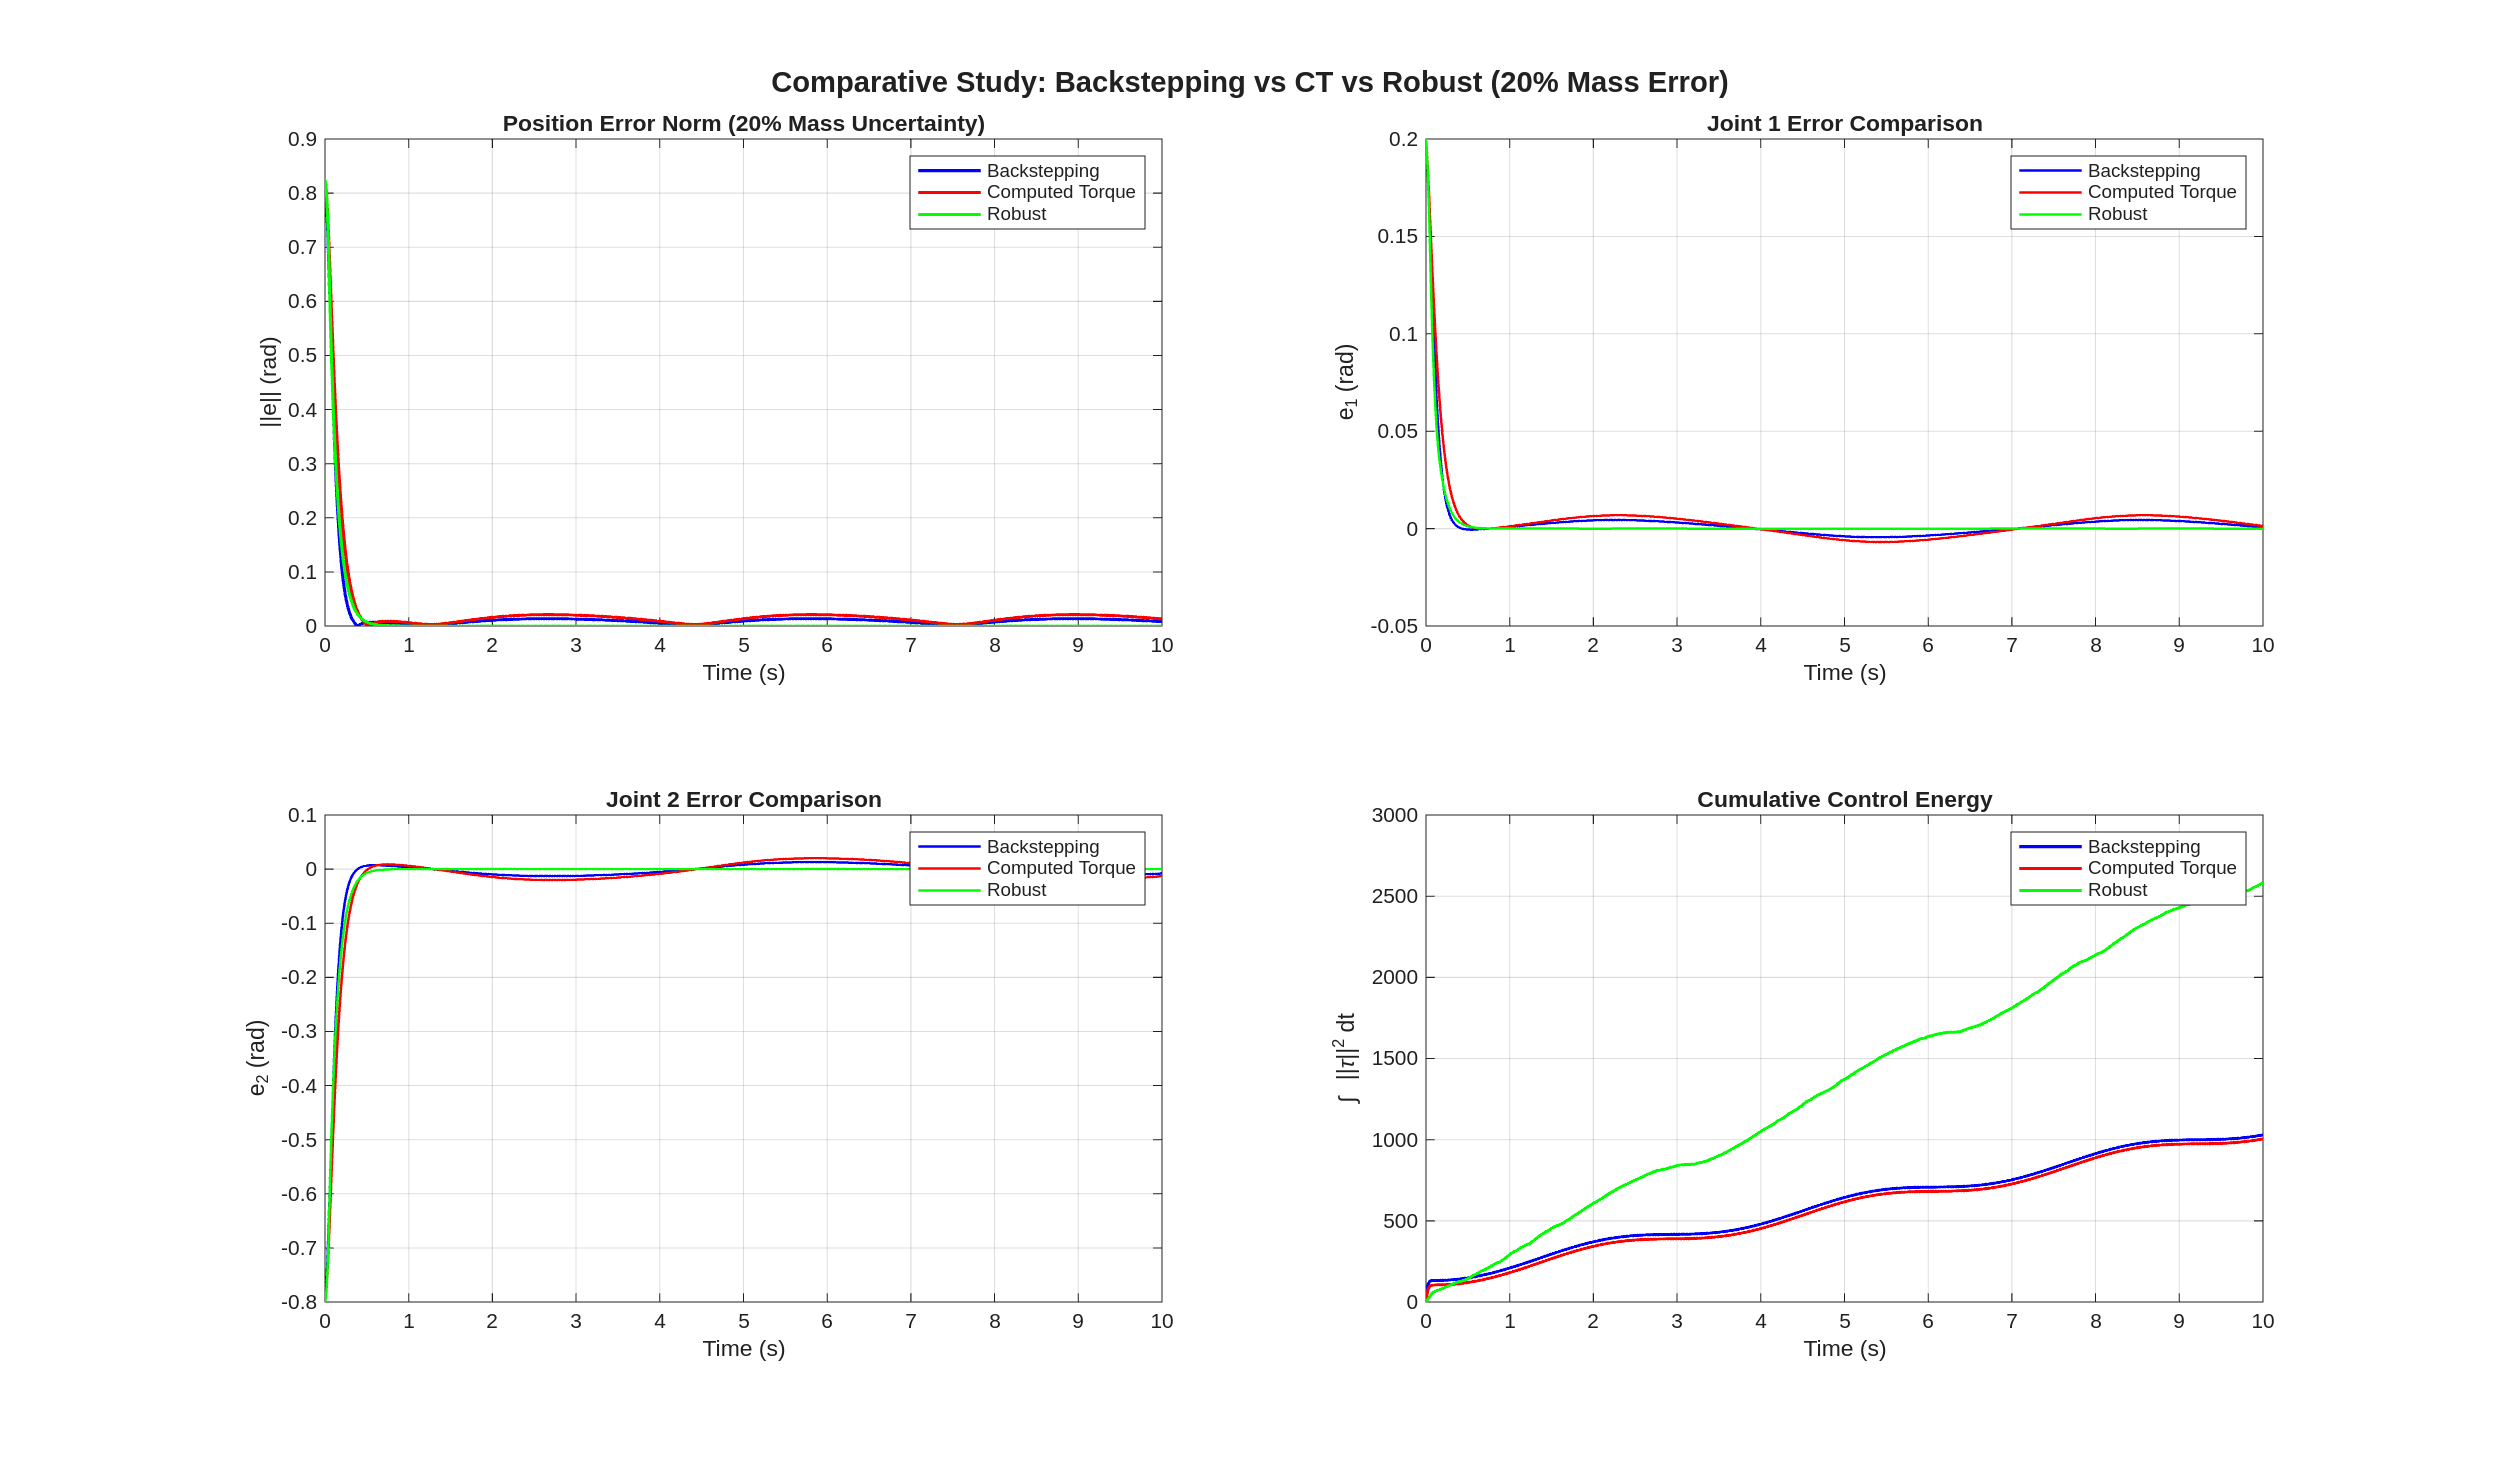
\includegraphics[width=0.92\textwidth,keepaspectratio]{images/week_07/Comparative_Study_With_Model_Uncertainty.png}
    \caption{Comparative study with model uncertainty.}
\end{figure}

\begin{figure}[ht]
    \centering
    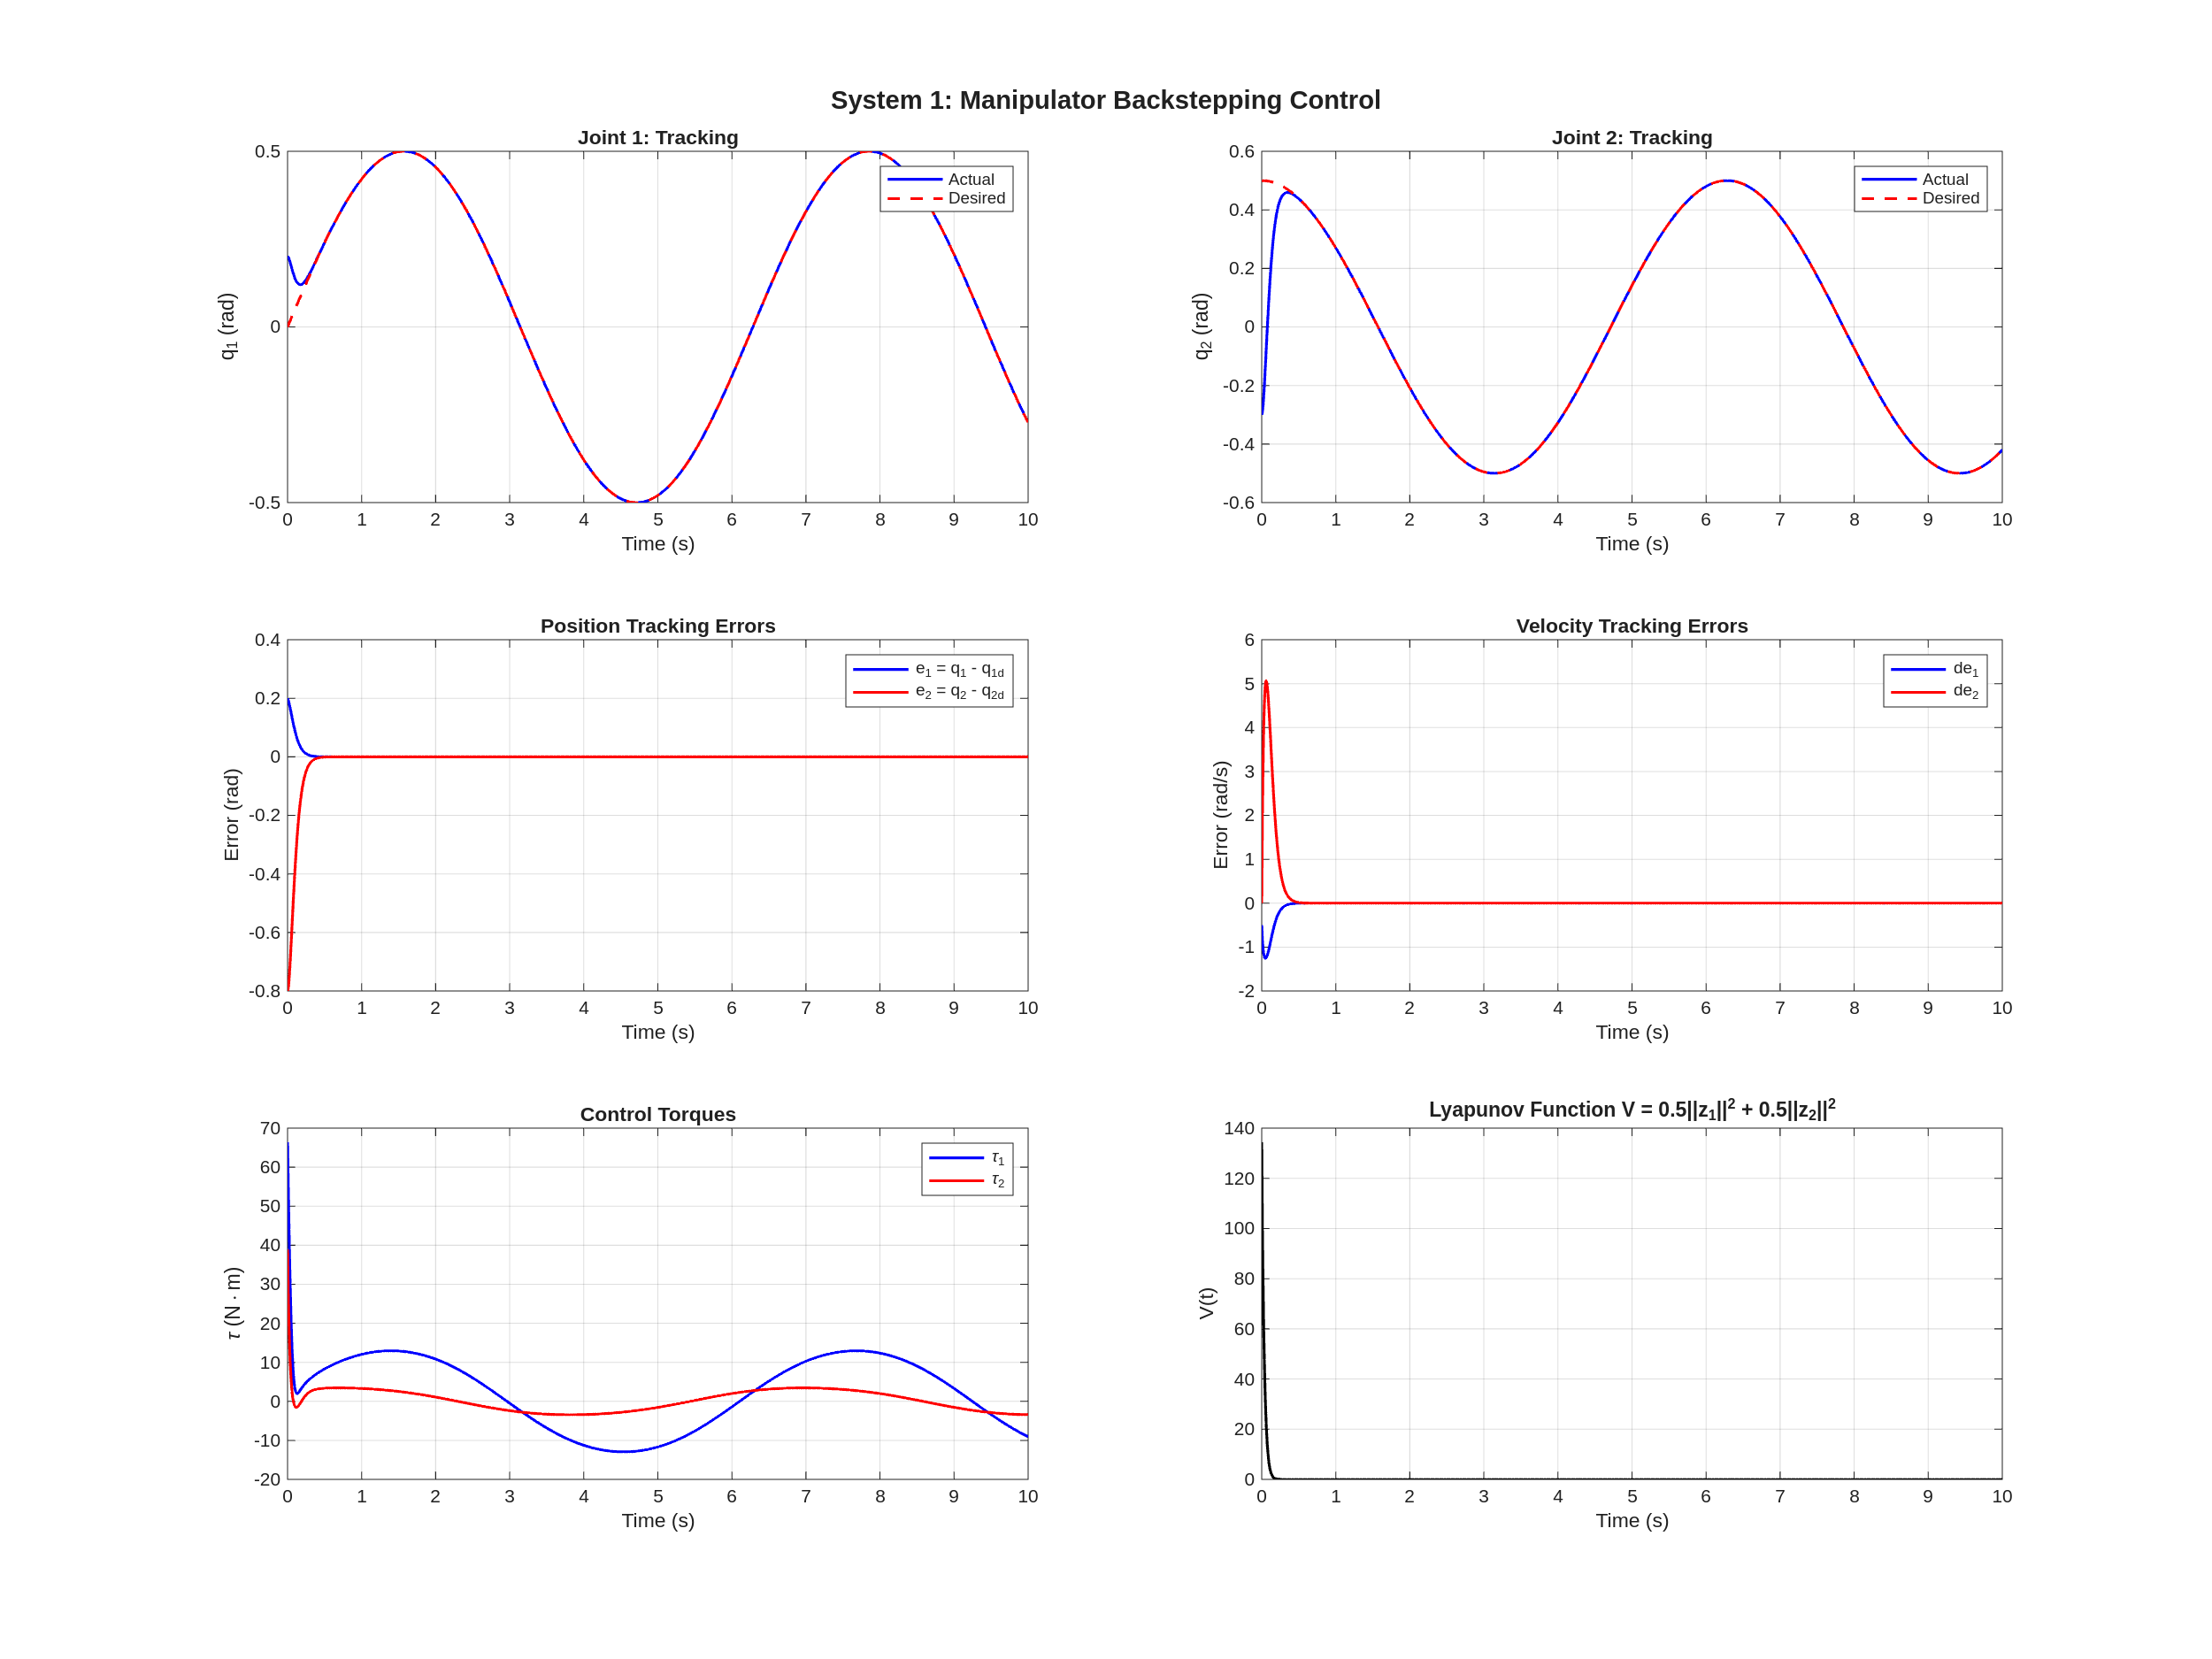
\includegraphics[width=0.92\textwidth,keepaspectratio]{images/week_07/Manipulator_Backstepping_Control.png}
    \caption{Manipulator backstepping control.}
\end{figure}

\begin{figure}[ht]
    \centering
    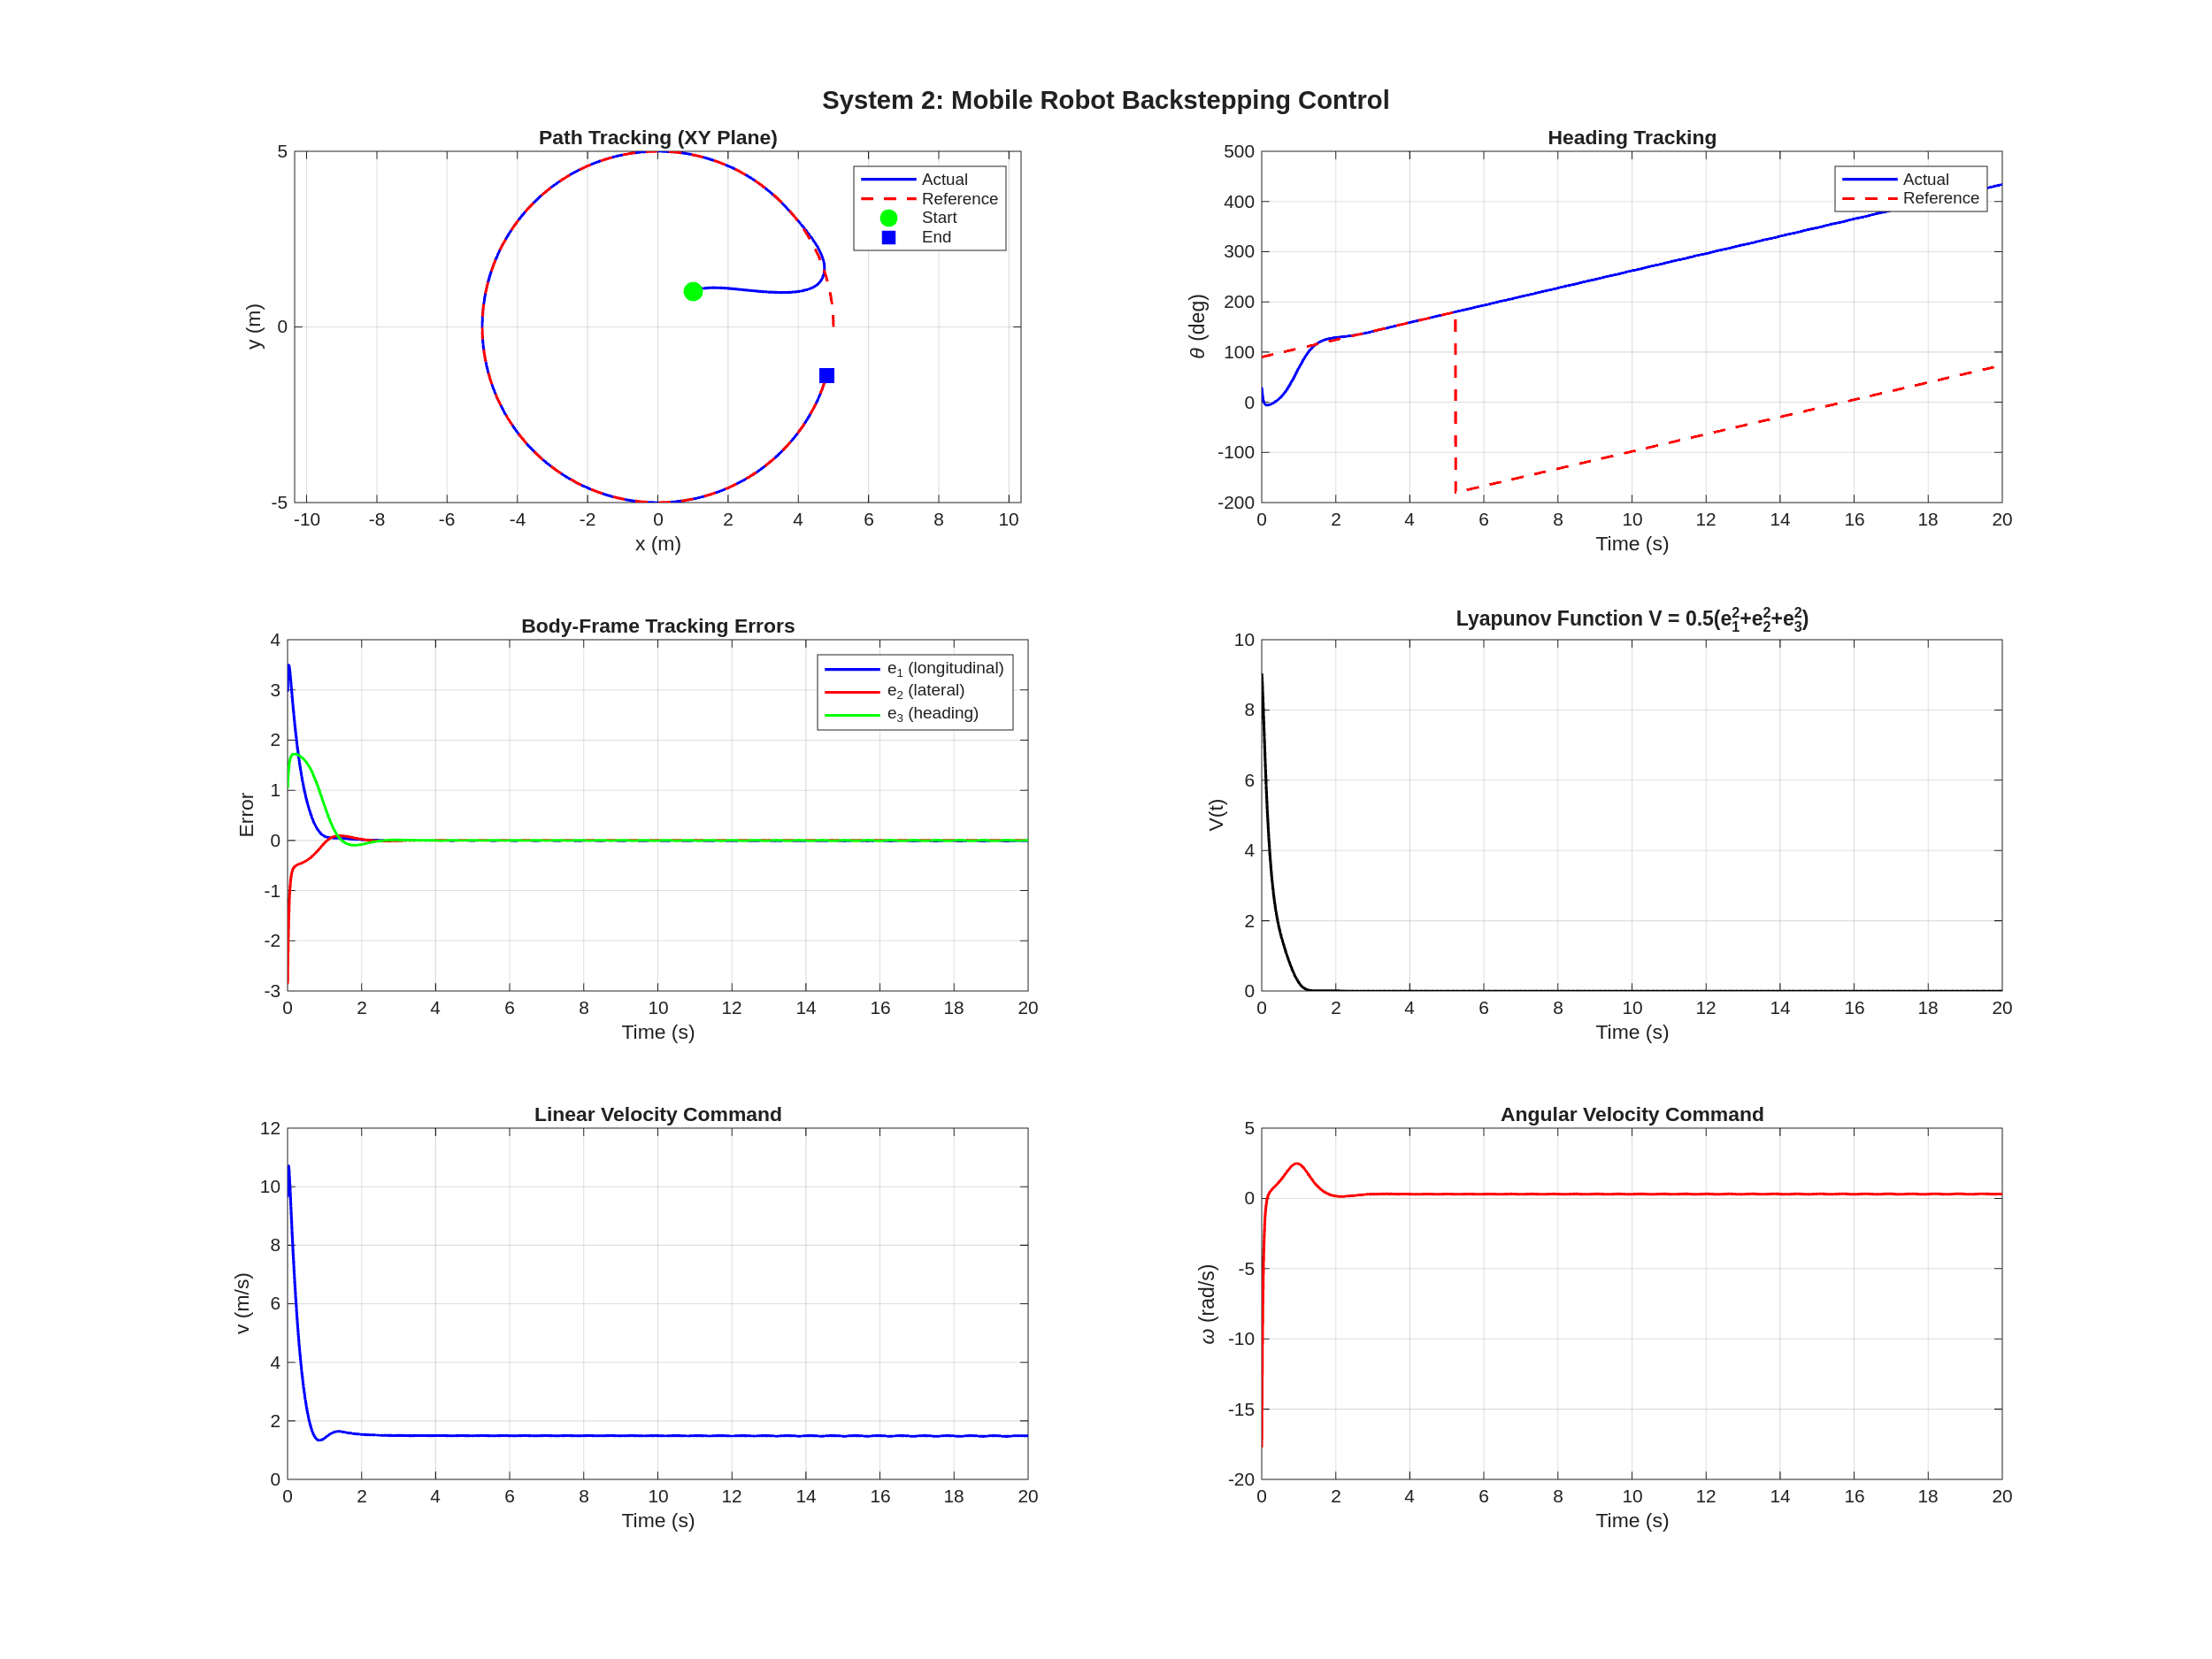
\includegraphics[width=0.92\textwidth,keepaspectratio]{images/week_07/Mobile_Robot_Backstepping_Control.png}
    \caption{Mobile robot backstepping control.}
\end{figure}

\begin{figure}[ht]
    \centering
    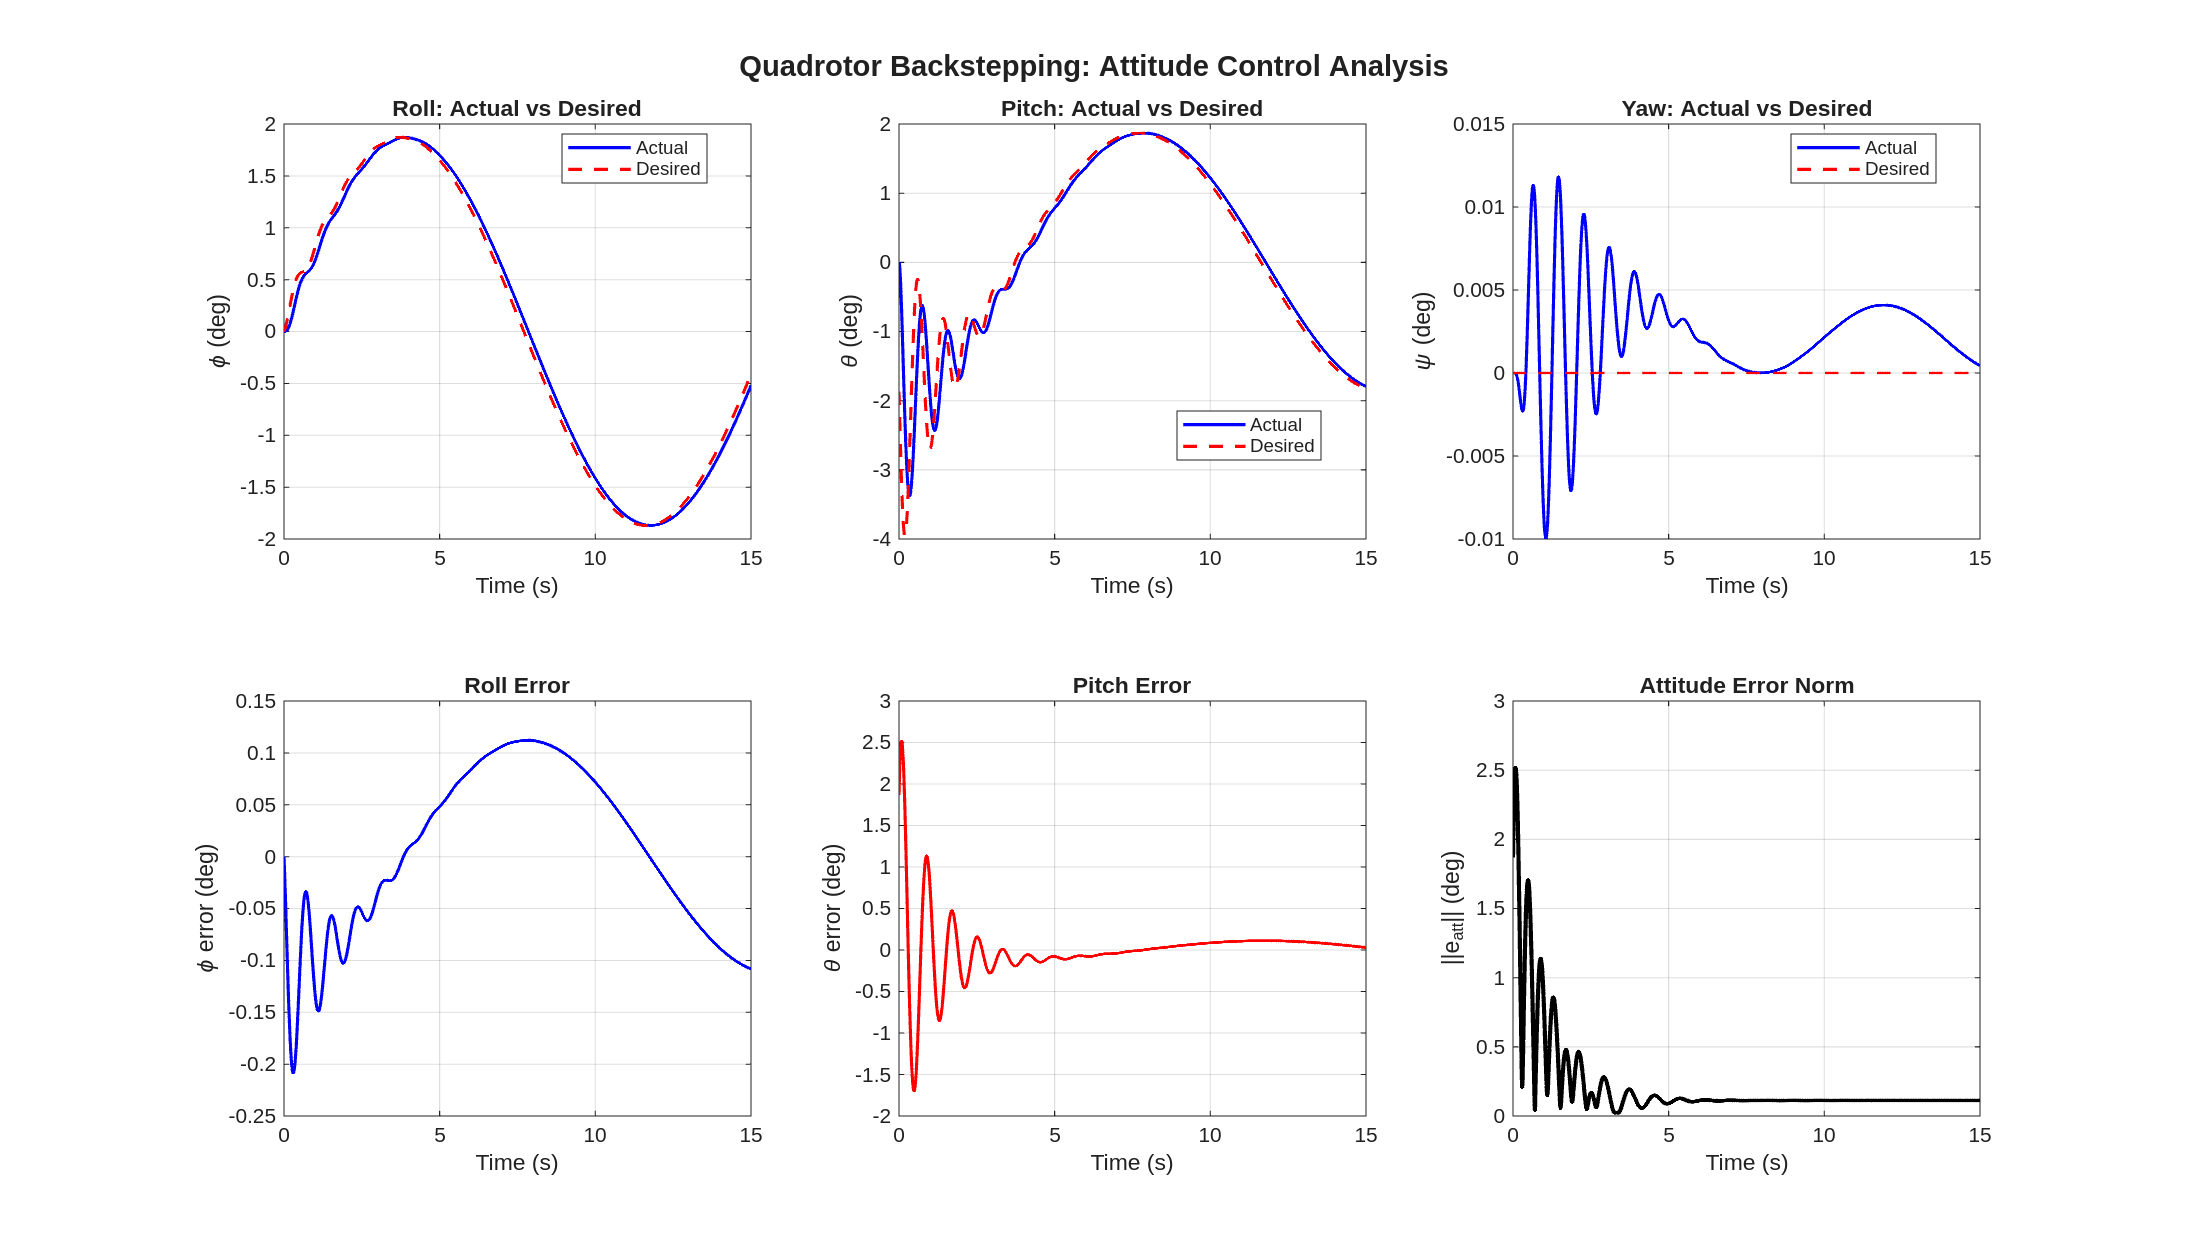
\includegraphics[width=0.92\textwidth,keepaspectratio]{images/week_07/Quad_Attitude_Control.png}
    \caption{Quad attitude control.}
\end{figure}

\begin{figure}[ht]
    \centering
    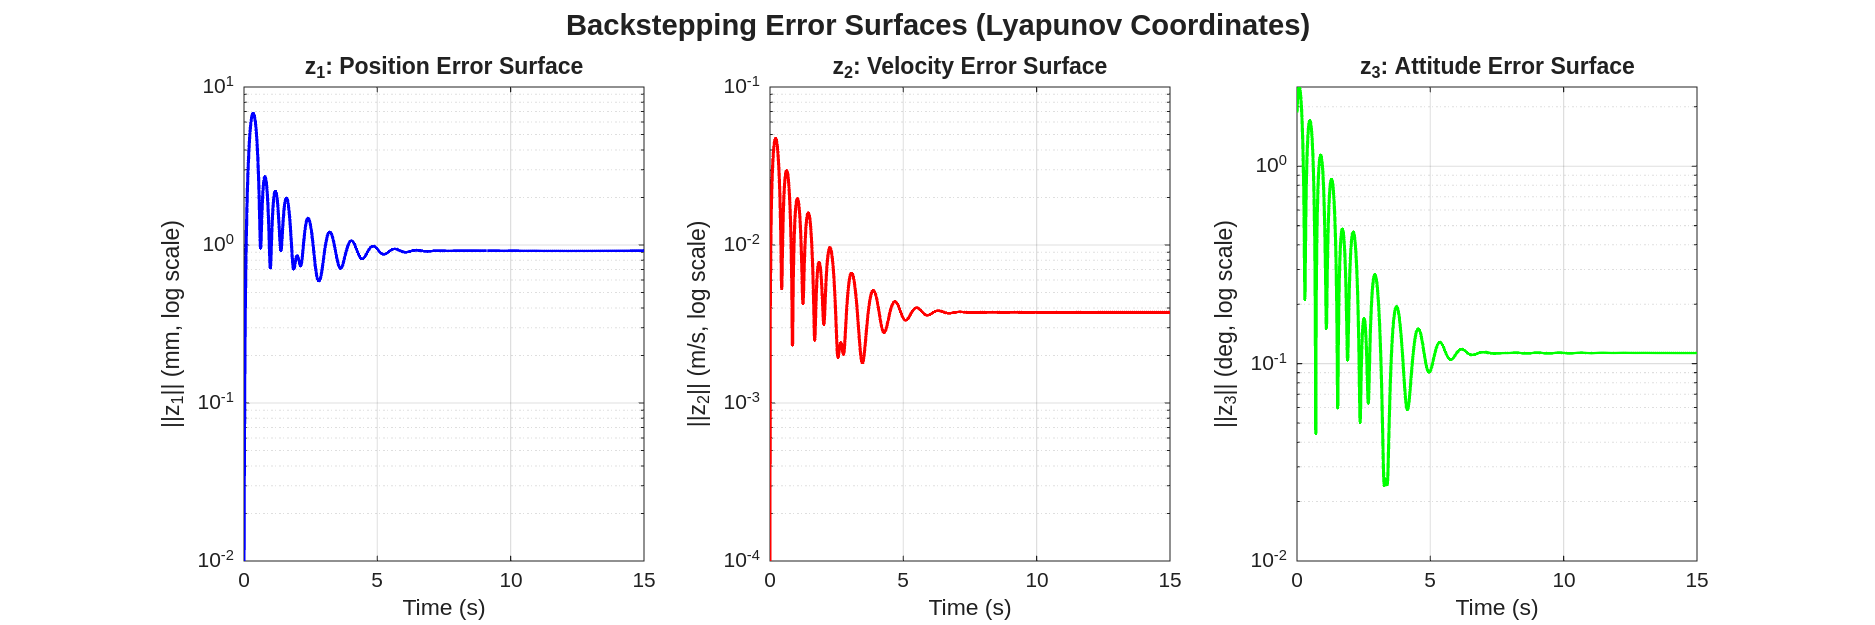
\includegraphics[width=0.92\textwidth,keepaspectratio]{images/week_07/Quad_Backstepping_Errors.png}
    \caption{Quad backstepping errors.}
\end{figure}

\begin{figure}[ht]
    \centering
    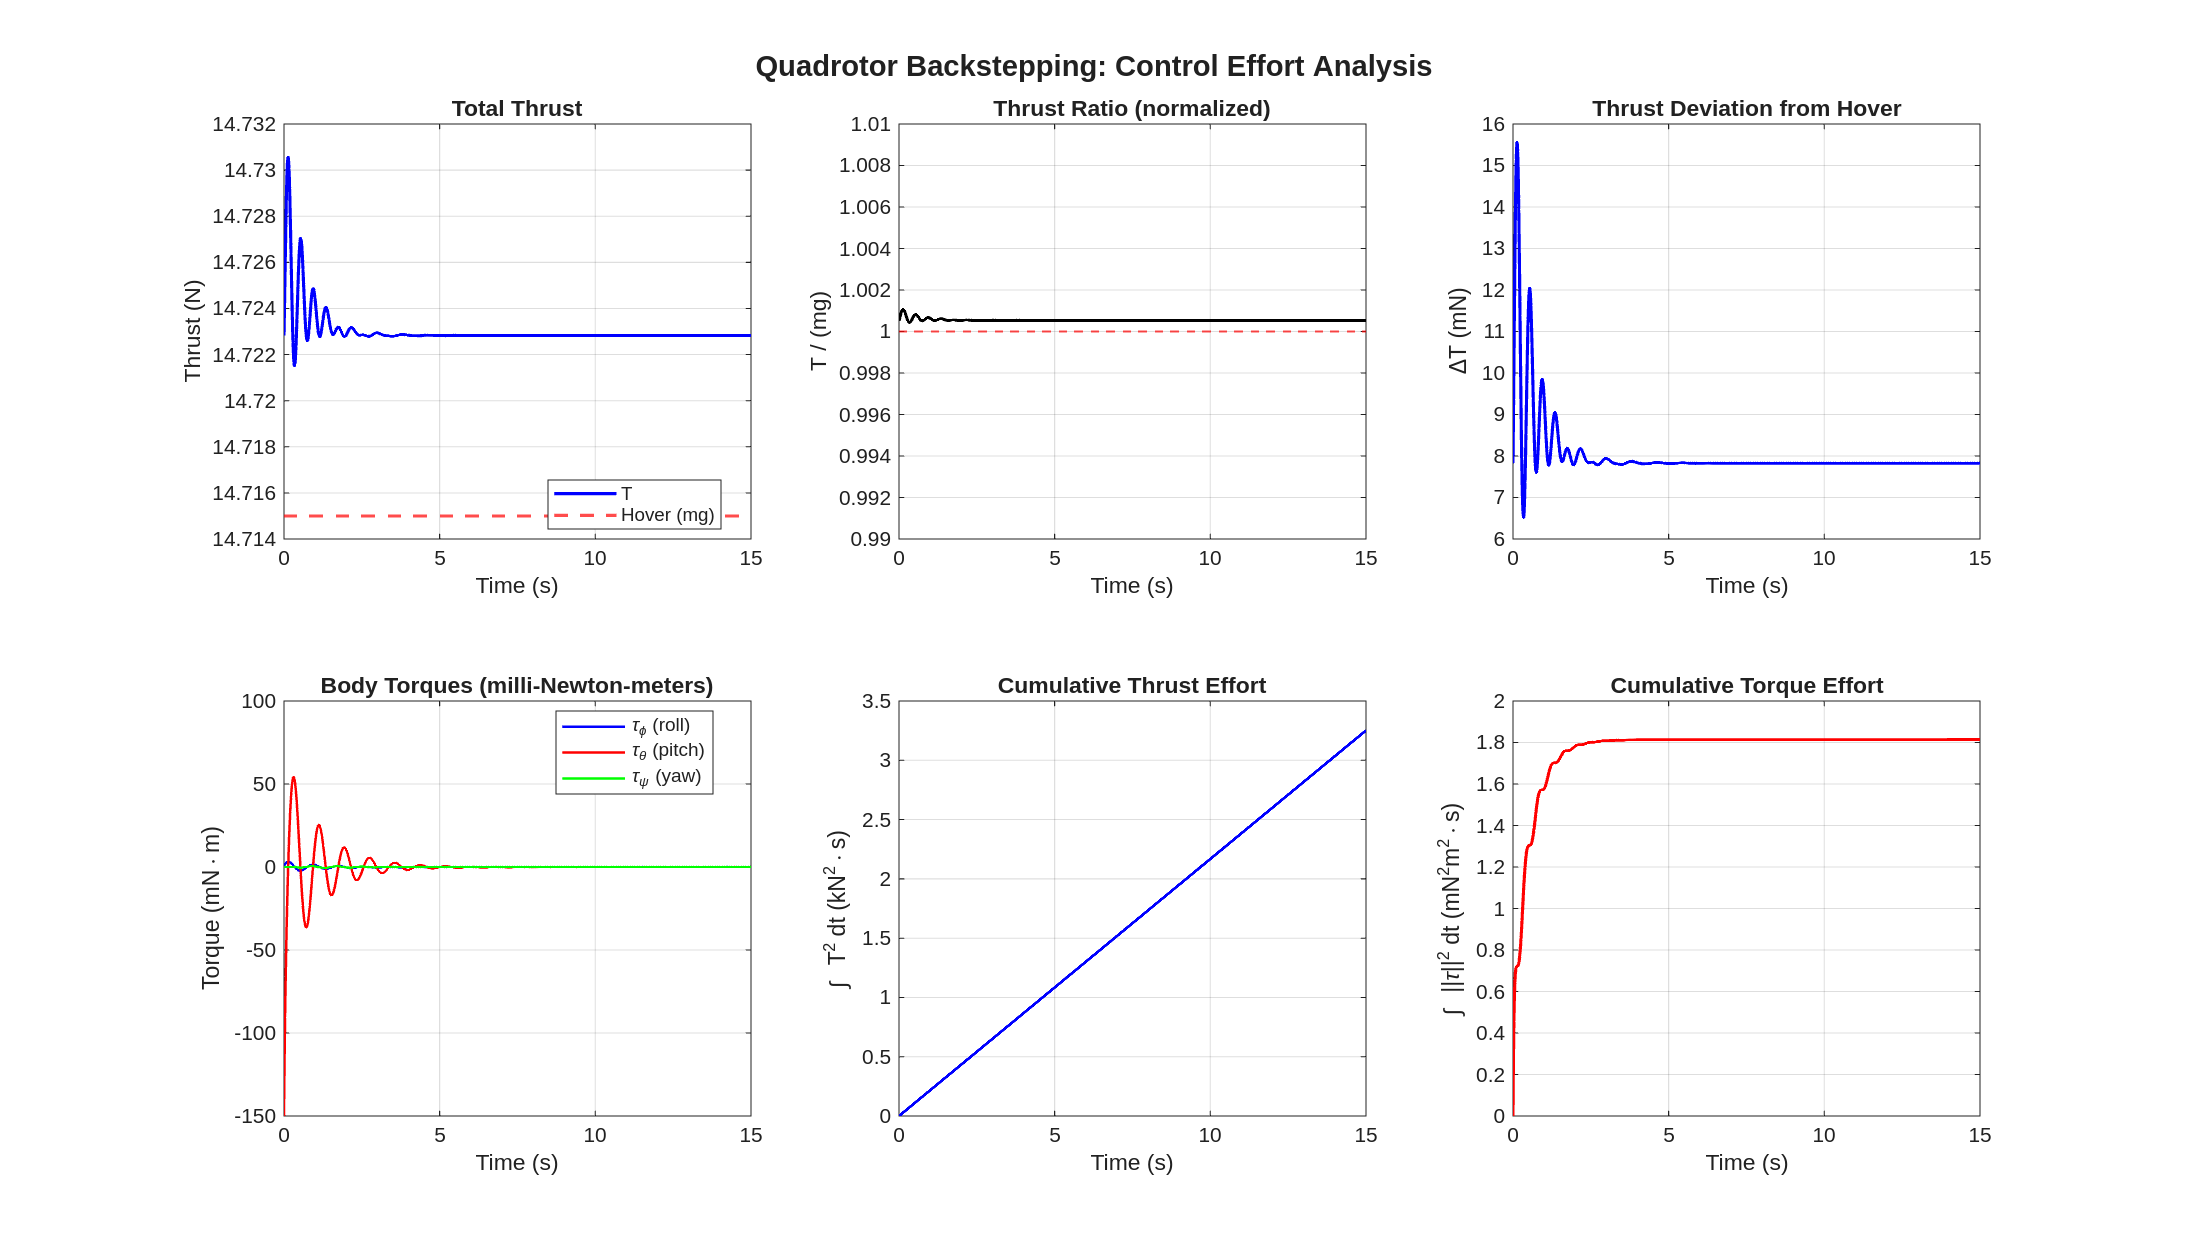
\includegraphics[width=0.92\textwidth,keepaspectratio]{images/week_07/Quad_Control_Effort.png}
    \caption{Quad control effort.}
\end{figure}

\begin{figure}[ht]
    \centering
    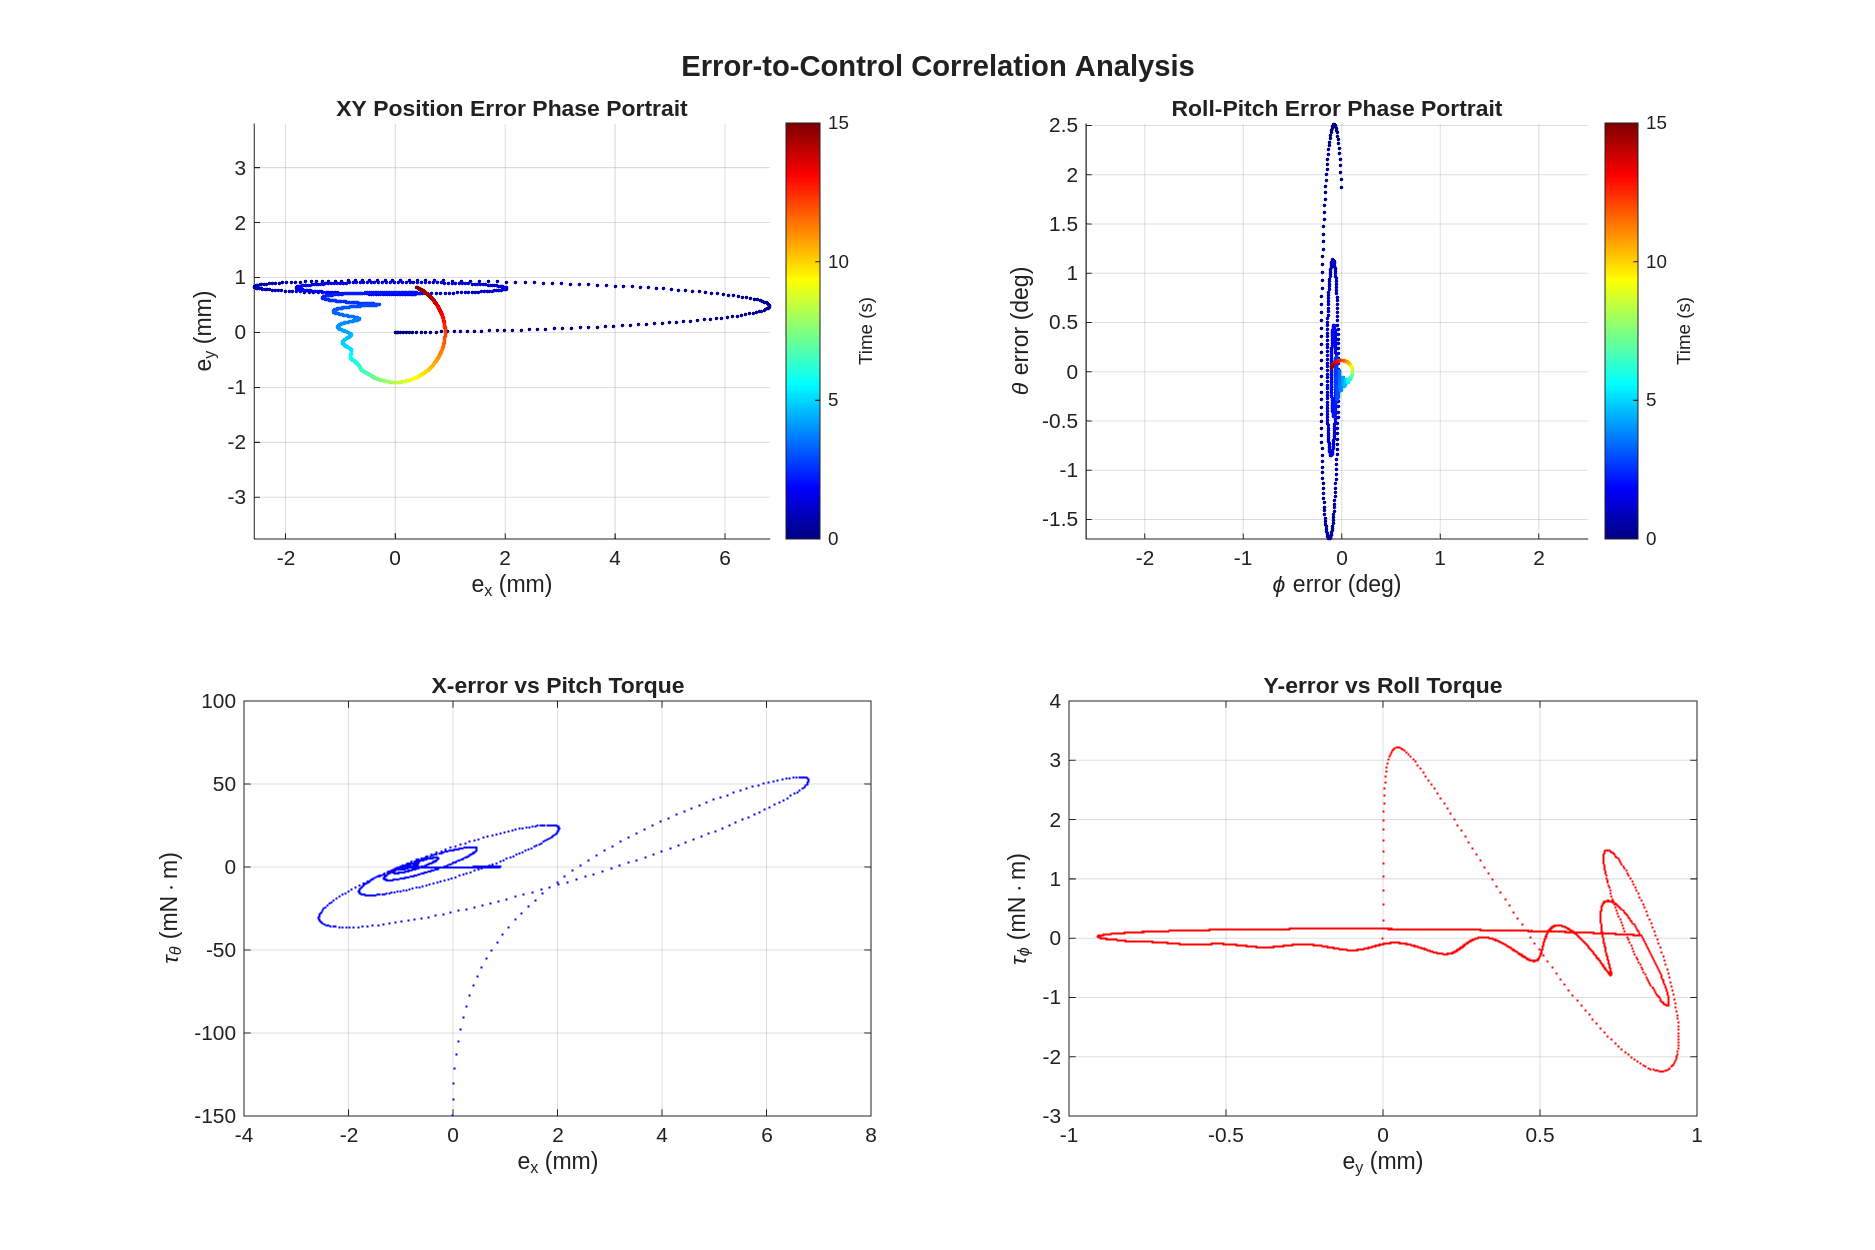
\includegraphics[width=0.92\textwidth,keepaspectratio]{images/week_07/Quad_Error_Control_Correlation.png}
    \caption{Quad error control correlation.}
\end{figure}

\begin{figure}[ht]
    \centering
    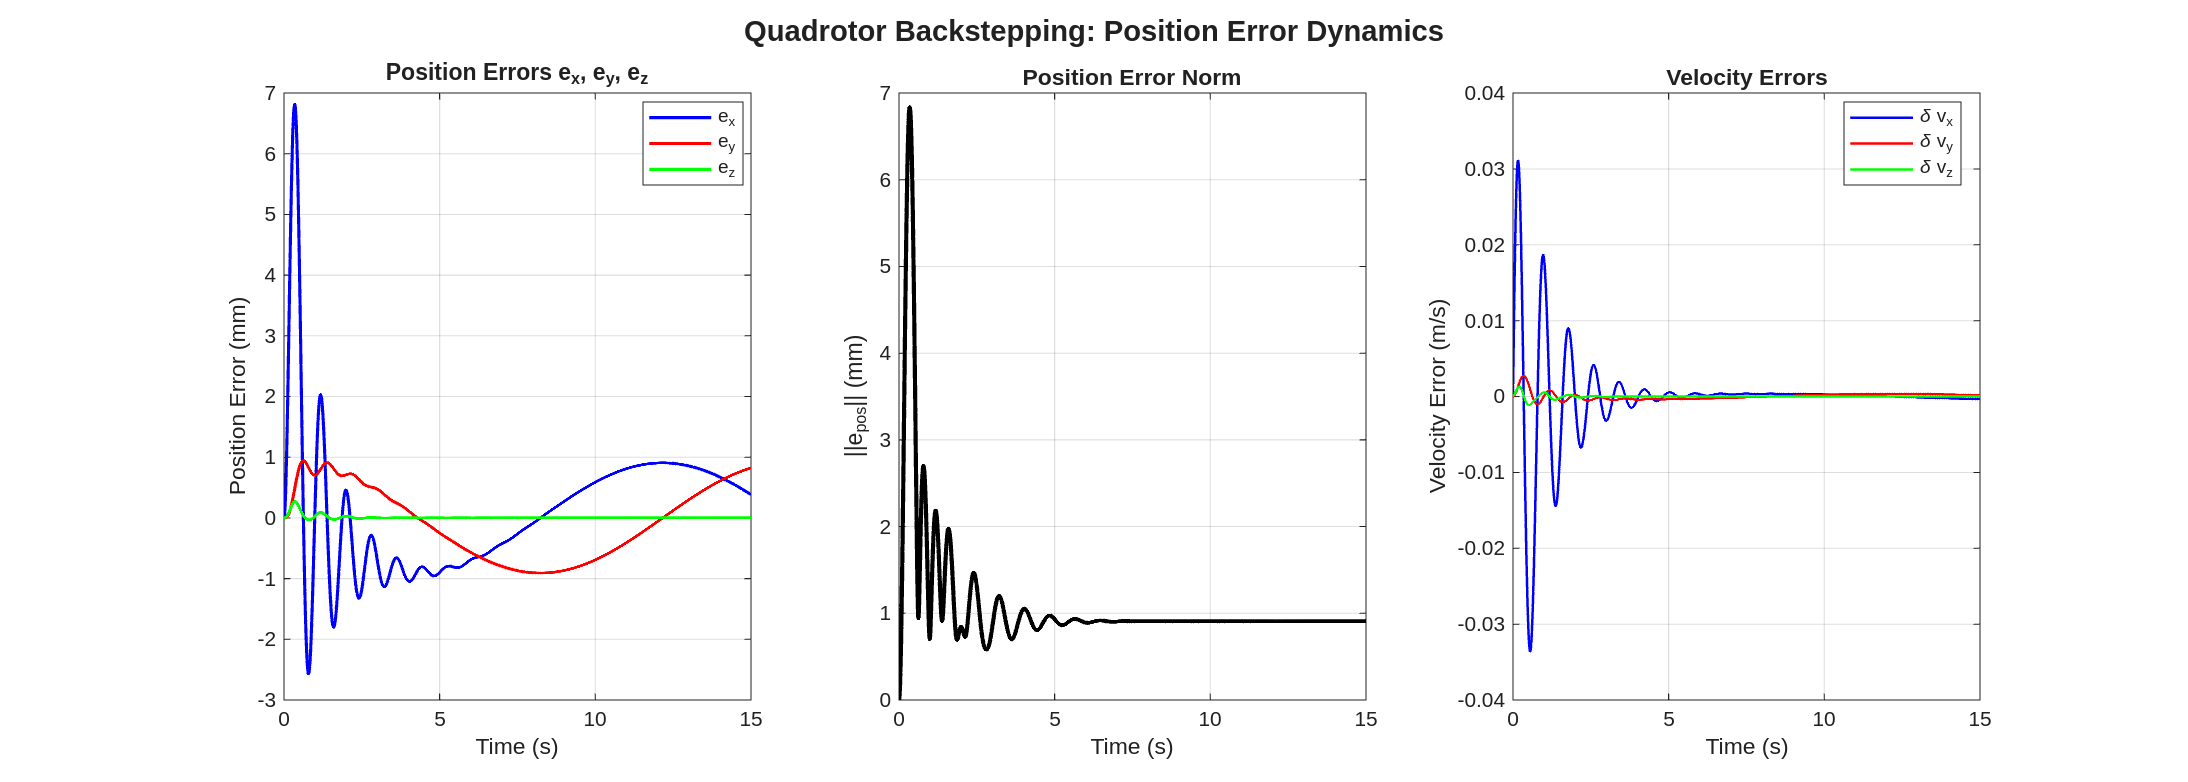
\includegraphics[width=0.92\textwidth,keepaspectratio]{images/week_07/Quad_Position_Error_Dynamics.png}
    \caption{Quad position error dynamics.}
\end{figure}

\begin{figure}[ht]
    \centering
    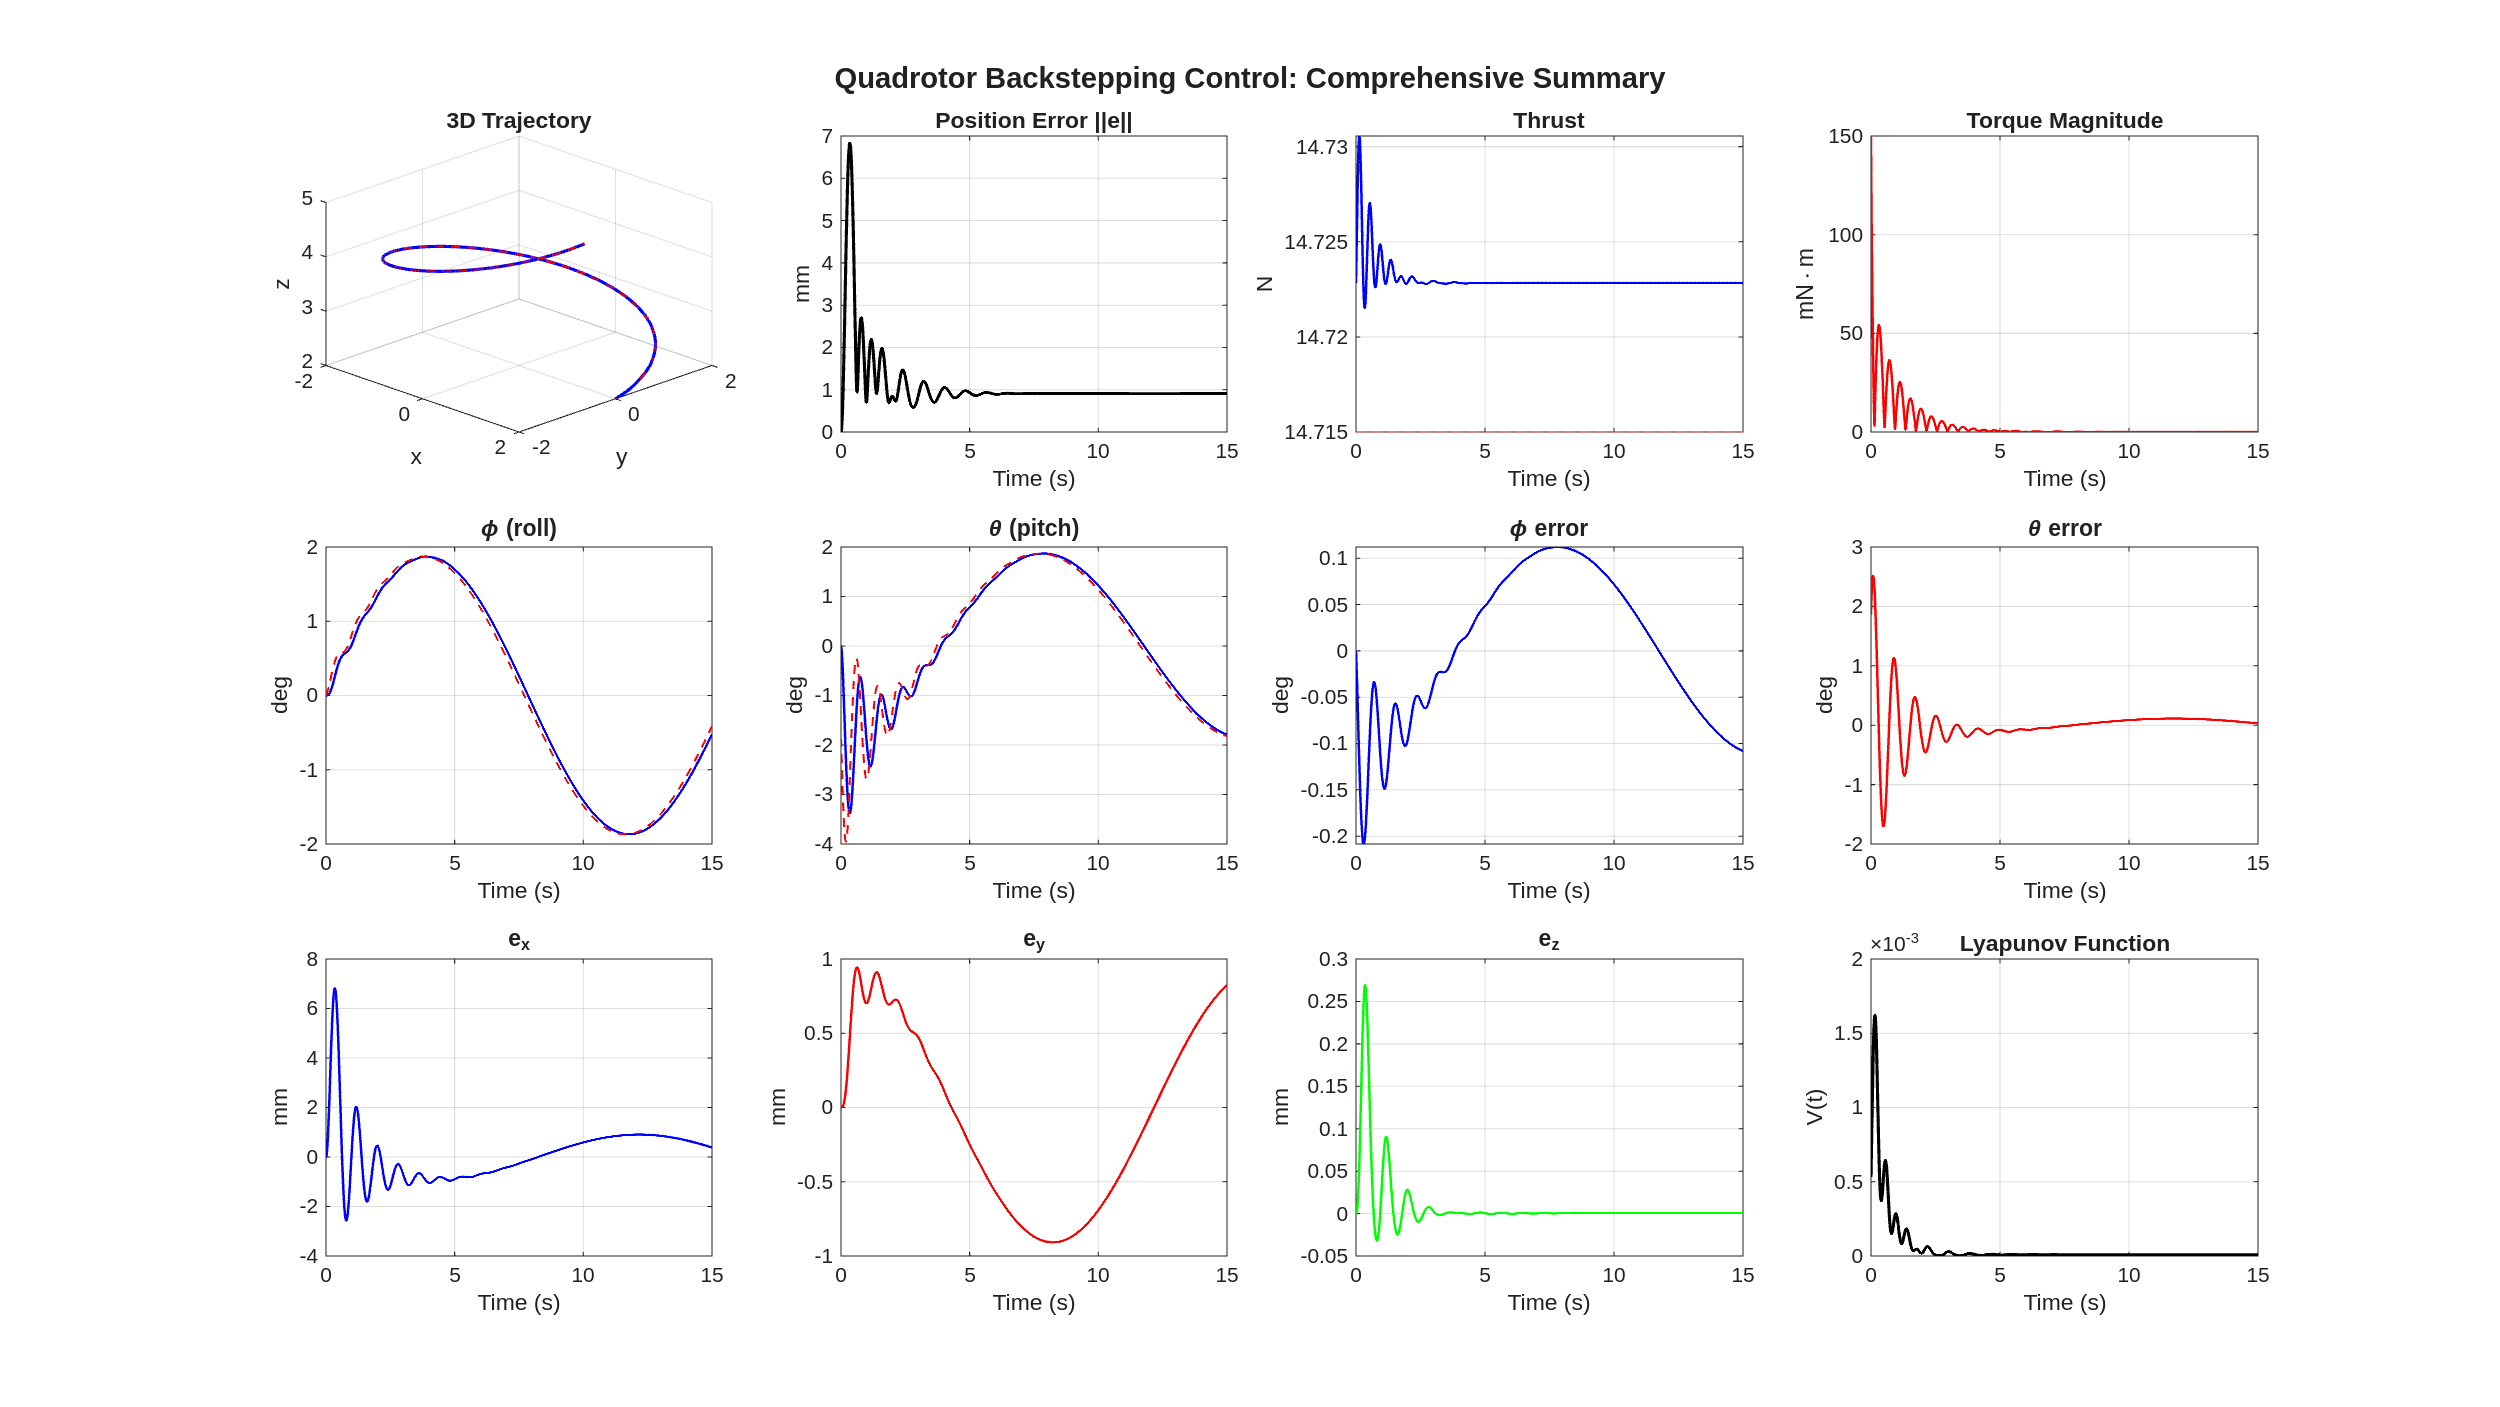
\includegraphics[width=0.92\textwidth,keepaspectratio]{images/week_07/Quad_Summary.png}
    \caption{Quad summary.}
\end{figure}

\begin{figure}[ht]
    \centering
    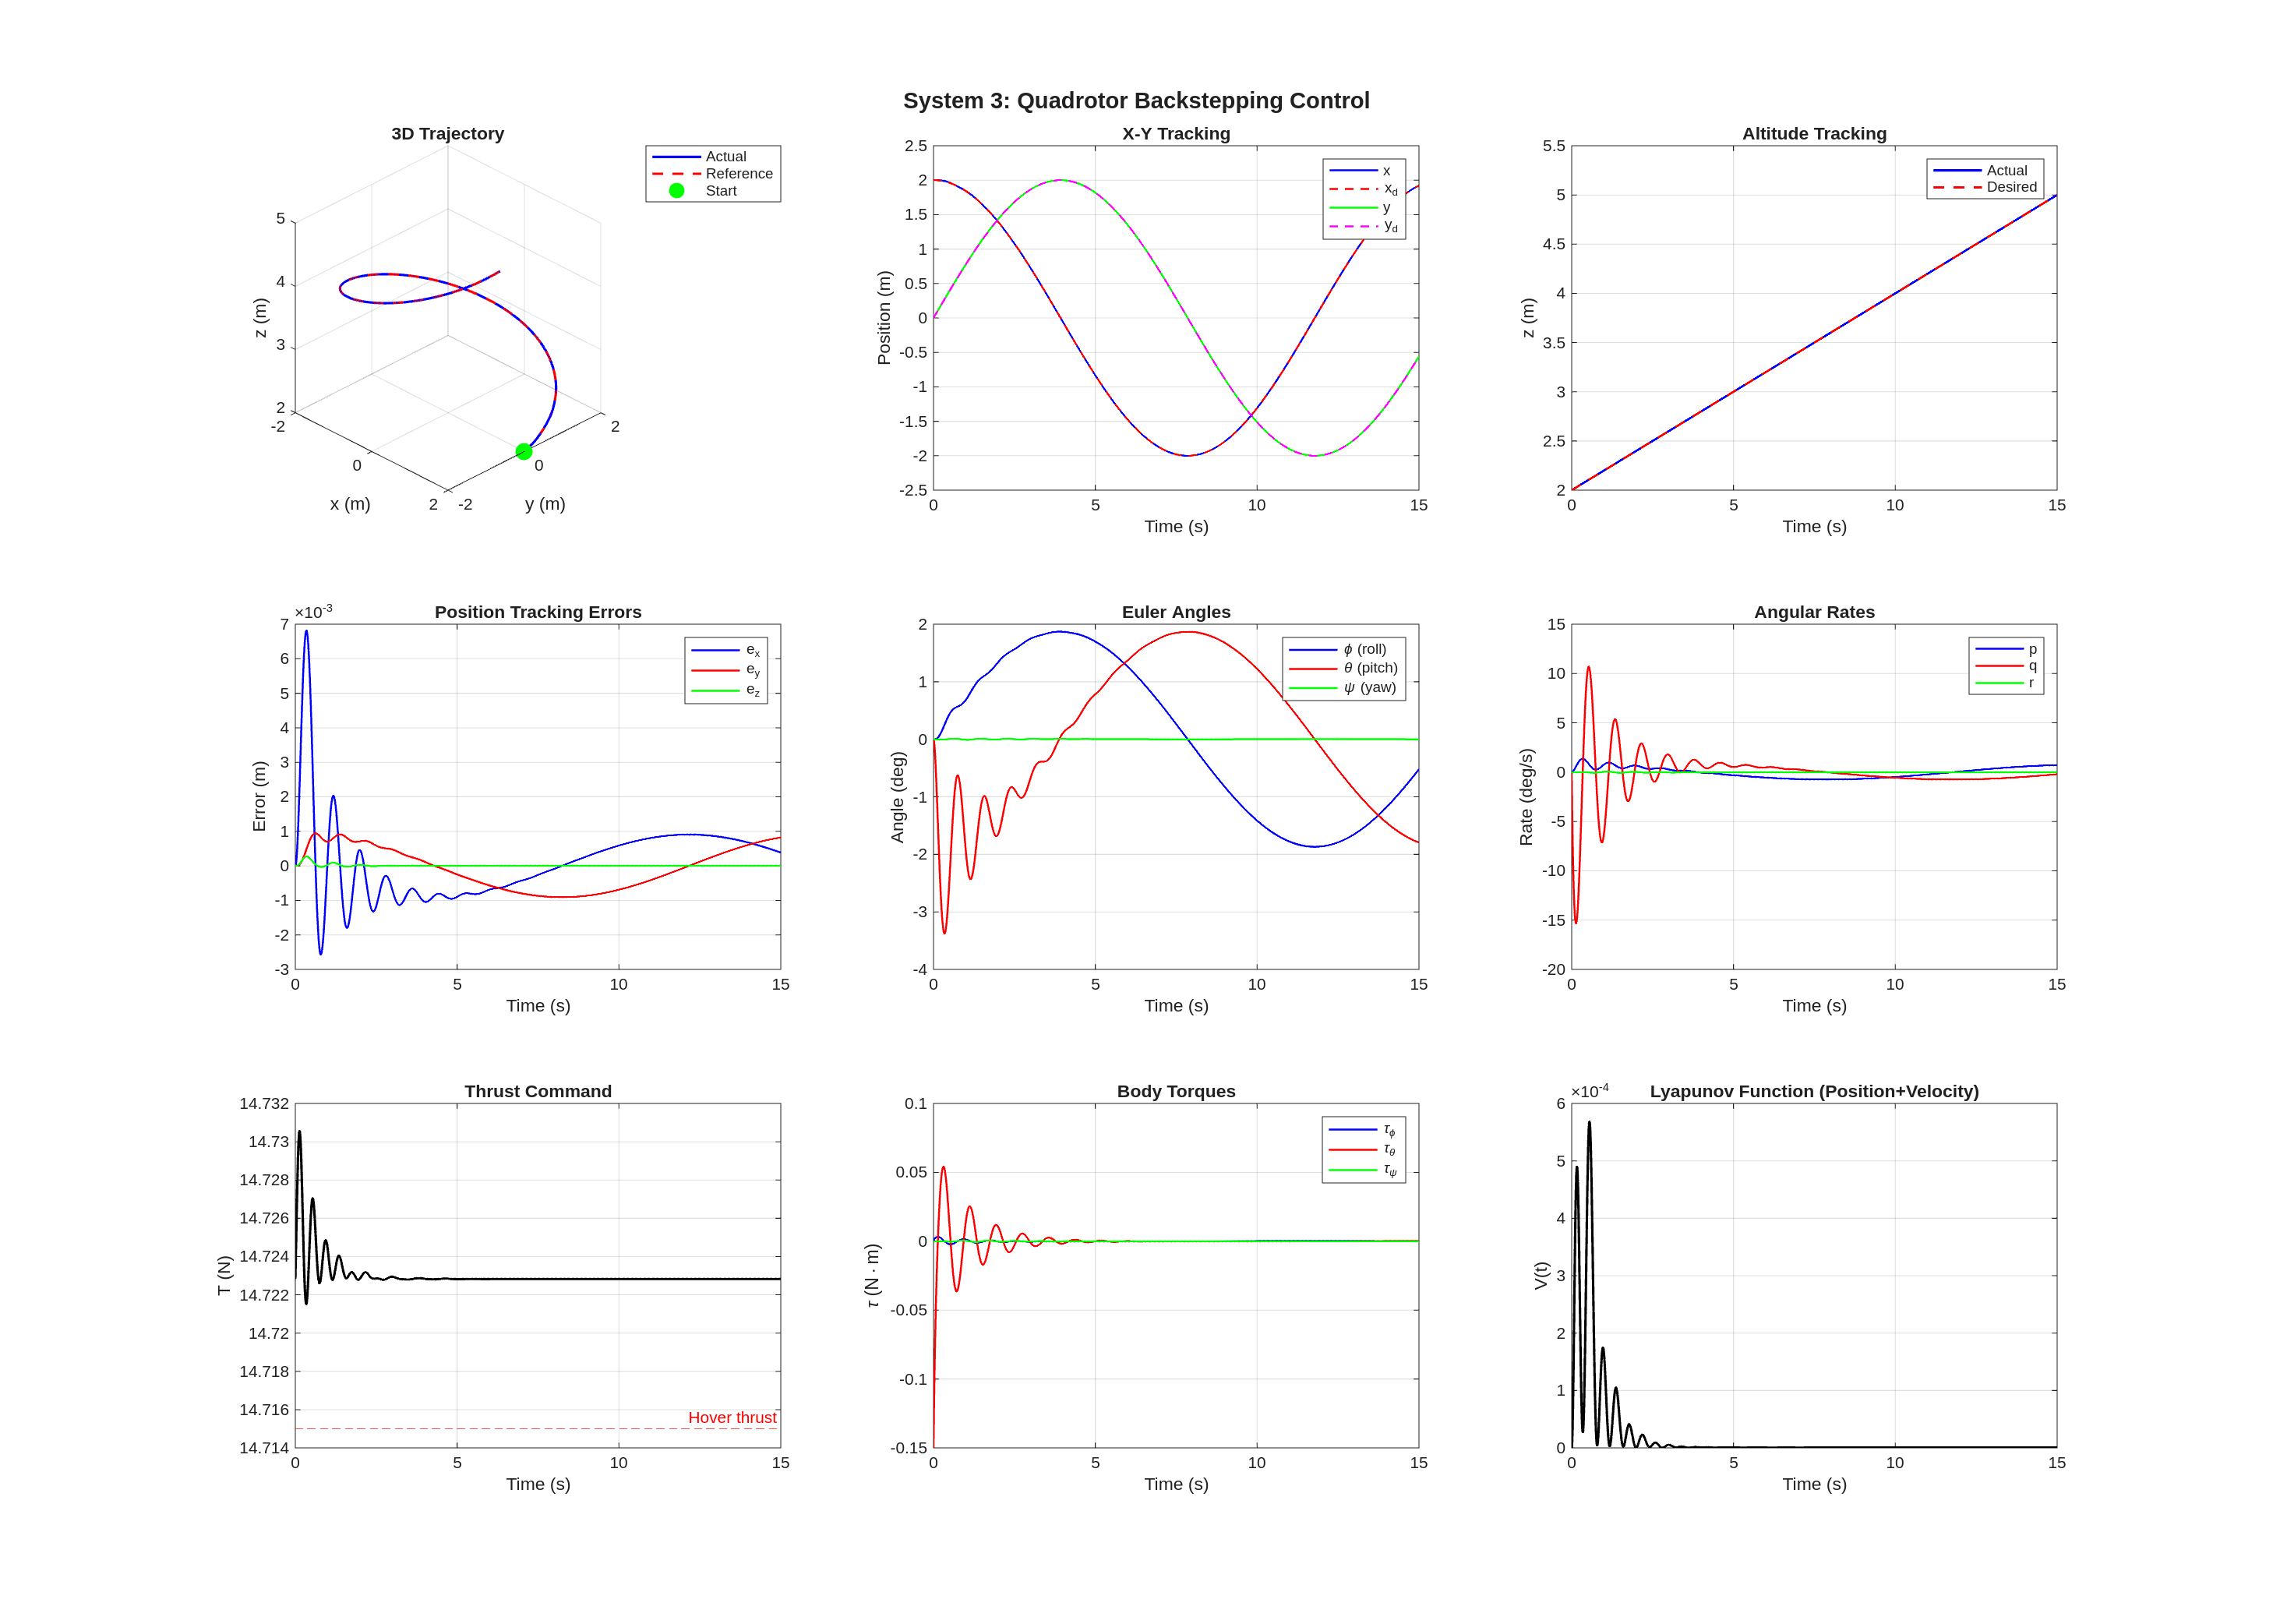
\includegraphics[width=0.92\textwidth,keepaspectratio]{images/week_07/Quadrotor_Backstepping_Control.png}
    \caption{Quadrotor backstepping control.}
\end{figure}

\section{Summary and Next Steps}

\subsection{Hands-on Activities \& Quiz}

\subsection{Activity 1: Gain Tuning for Manipulator Backstepping (10 min)}

Run \texttt{backstepping\_control\_simulation.m} and observe the manipulator plots.
Then modify the gains and re-run:

\begin{enumerate}
\tightlist
\item
  Set \(k_1 = 50, \; k_2 = 5\) (position gain much larger than velocity gain).
\item
  Set \(k_1 = 5, \; k_2 = 50\) (velocity gain much larger than position gain).
\item
  Set \(k_1 = k_2 = 25\) (balanced gains).
\end{enumerate}

\textbf{Expected observations:}

\begin{itemize}
\tightlist
\item
  \textbf{\(k_1 \gg k_2\):} Aggressive position correction generates large desired velocity changes.
  The velocity loop cannot track them fast enough, causing oscillatory or even unstable behaviour.
  The virtual control \(\alpha_1\) demands more than the torque loop can deliver.
\item
  \textbf{\(k_2 \gg k_1\):} The velocity error \(z_2\) converges quickly, but the position
  error \(z_1\) converges slowly because \(k_1\) is small. The system is overdamped
  with sluggish position tracking.
\item
  \textbf{\(k_1 \approx k_2\):} Balanced convergence rates for both loops. This is
  generally the best choice for smooth, fast tracking.
\end{itemize}

\subsection{Activity 2: Comparative Study (15 min)}

The MATLAB file includes a comparison of backstepping vs. computed torque vs. robust control
on the manipulator with model uncertainty (20\% mass error). Observe:

\begin{itemize}
\tightlist
\item
  Which controller has the smallest steady-state error?
\item
  Which controller has the smoothest control signal?
\item
  Which controller uses the least energy (smallest \(\int \|\tau\|^2 \, dt\))?
\end{itemize}

\subsubsection{Quiz --- Virtual Control Design}

\textbf{Q1:} Given the system \(\dot{x}_1 = x_1^2 + x_2\), \(\dot{x}_2 = x_2 + u\),
design a backstepping controller to stabilise \(x_1 = 0\).

\emph{Answer sketch:}

\begin{itemize}
\tightlist
\item
  Step 1: \(z_1 = x_1\), \(\dot{z}_1 = x_1^2 + x_2\).
  Choose \(\alpha_1 = -x_1^2 - k_1 x_1\) so that \(\dot{V}_1 = -k_1 x_1^2 + x_1 z_2\).
\item
  Step 2: \(z_2 = x_2 - \alpha_1\), \(\dot{z}_2 = x_2 + u - (2x_1)(x_1^2 + x_2) + k_1(x_1^2 + x_2)\).
  Choose \(u = -x_2 + \dot{\alpha}_1 - x_1 - k_2 z_2\).
\end{itemize}

\textbf{Q2:} In the two-step backstepping controller, what happens if we omit the
cross-coupling term \(-z_1\) from the torque law? Is stability still guaranteed?

\emph{Answer:} Without \(-z_1\), the Lyapunov derivative becomes
\(\dot{V}_2 = -k_1 z_1^2 - k_2 z_2^2 + z_1^T z_2\). The cross-term \(z_1^T z_2\) can be
positive, so \(\dot{V}_2\) is not guaranteed negative semi-definite. Stability is only ensured
if \(k_1 k_2 > \frac{1}{4}\) (by Young\textquotesingle s inequality), but the stability margin is reduced.
The systematic backstepping design avoids this issue entirely.

\textbf{Q3:} Why does the quadrotor need four backstepping steps while the
manipulator only needs two?

\emph{Answer:} The quadrotor has a four-level cascade:
position → velocity → orientation → angular rate, each acting as a virtual control
for the previous level. The manipulator only has two levels (position → velocity) because
the torque directly enters the velocity dynamics via \(M^{-1}\tau\). The number of backstepping
steps equals the relative degree from the output to the input.

\subsection{Summary: Comparison of All Five Control Methods}

\begin{table}[ht]\footnotesize\centering
\adjustbox{max width=\textwidth,max totalheight=0.85\textheight}{%
\begin{tabular}{llllll}

\topruleAspect & Computed Torque (Wk1) & MPC (Wk2) & Adaptive (Wk3) & Robust (Wk4) & Backstepping (Wk5) \\
\midrule\bottomrule\textbf{Core idea} & Cancel nonlinearity, impose linear error dynamics & Optimise predicted trajectory over finite horizon & On-line parameter estimation + control & Dominate worst-case bounded uncertainty & Recursive Lyapunov design through cascade structure \\
\textbf{Model requirement} & Exact model needed & Prediction model needed & Structure known, parameters unknown & Nominal model + uncertainty bound & Strict-feedback structure required \\
\textbf{Lyapunov function} & Implicit (linear closed-loop) & Cost function (not standard Lyapunov) & \(V = \frac{1}{2}s^T M s + \frac{1}{2}\tilde{\theta}^T\Gamma^{-1}\tilde{\theta}\) & \(V = \frac{1}{2}s^T M s\) & \(V = \sum \frac{1}{2}z_i^T W_i z_i\) (constructed step-by-step) \\
\textbf{Handles constraints} & No & Yes (core feature) & No (standard form) & No & No (standard form) \\
\textbf{Robustness} & Poor (sensitive to model errors) & Moderate (depends on model accuracy) & Good (adapts to parametric uncertainty) & Excellent (designed for uncertainty) & Good (Lyapunov-guaranteed; can add adaptation) \\
\textbf{Computation} & Low (closed-form) & High (on-line optimisation) & Moderate (adaptation law update) & Low (closed-form) & Moderate (derivatives of virtual controls) \\
\textbf{Key advantage} & Simple, well-understood & Handles constraints and preview & Self-tuning for unknown parameters & Guaranteed performance under uncertainty & Systematic design with constructive stability proof \\
\textbf{Key limitation} & No robustness to model error & Computational cost, model dependence & Needs persistent excitation, structured uncertainty & Conservative (worst-case design), chattering & Complexity explosion in \(\dot{\alpha}_i\) for high-order systems \\
\textbf{Control law form} & \(\tau = M(q)[\ddot{q}_d + K_D\dot{e} + K_P e] + C\dot{q} + G\) & \(u^* = \arg\min_{u} \sum_{k} \|x_k - x_r\|^2_Q + \|u_k\|^2_R\) & \(\tau = Y(q,\dot{q},\dot{q}_r,\ddot{q}_r)\hat{\theta} - K_D s\) & \(\tau = \hat{M}\ddot{q}_r + \hat{C}\dot{q}_r + \hat{G} - K_D s + \rho\frac{s}{\|s\|}\) & \(\tau = M[\ddot{q}_d - K_1\dot{z}_1 - K_2 z_2] + C\alpha_1 + G - z_1\) \\
\end{tabular}}
\end{table}


\textbf{Figure 8:} Side-by-side comparison of feedback linearization (cancels all nonlinearities) versus backstepping (exploits useful nonlinearities with constructive Lyapunov guarantees).

\textbf{Key takeaway:} Backstepping provides a \emph{systematic, constructive} methodology
for designing stabilising controllers for nonlinear systems in strict-feedback form.
Unlike computed torque, it does not blindly cancel all nonlinearities.
Unlike robust control, it does not require conservative worst-case bounds.
Its main challenge --- the "explosion of terms" as \(\dot{\alpha}_i\) grows with each step
--- can be addressed using \textbf{dynamic surface control} (a first-order filter on
each virtual control), which we may explore in future weeks.

\textbf{M.Sc. Control for Robots} --- AY 2025--26

Week 5: Backstepping Control --- Lecture Notes

These notes are for educational purposes.
Students are encouraged to verify all derivations independently.
   % Chapter 7: Backstepping Control (Week 7)
% ----- auto-generated from week_08/Week*.html via pandoc -----
\setchapterimage[6cm]{}
\setchapterpreamble[u]{\margintoc}
\chapter{Nonlinear Control Optimization for Robotic Systems}
\labch{week_08}

\section{Week 8: Nonlinear Control Optimization for Robotic Systems}\label{week-8-nonlinear-control-optimization-for-robotic-systems}}

From Pontryagin \& HJB to Optimized SMC, Adaptive, Robust, Backstepping, and NMPC

M.Sc. Control for Robots --- University of West London --- AY 2025--26\\
Week 8 of 12 (Control Theory Block) • Lecture + MATLAB Lab

\subsection{Section 1: Learning Outcomes}\label{section-1-learning-outcomes}}

By the end of this session, you will be able to:

\begin{itemize}
\tightlist
\item
  Explain why linear optimal control (LQR/LQG) is fundamentally insufficient for robotic systems whose dynamics are nonlinear
\item
  State the nonlinear optimal control problem and derive necessary conditions via Pontryagin\textquotesingle s Minimum Principle (PMP)
\item
  Formulate the nonlinear HJB equation and explain why direct solution is infeasible for robots
\item
  Describe direct transcription methods (single/multiple shooting, collocation) and apply iLQR / DDP and NMPC to a manipulator, mobile robot, and quadrotor
\item
  Pose the tuning of \textbf{sliding-mode}, \textbf{adaptive}, \textbf{robust}, \textbf{backstepping}, and \textbf{nonlinear MPC} controllers as constrained nonlinear optimization problems
\item
  Select appropriate decision variables, cost functionals, constraints, and solvers for each controller family
\item
  Interpret Pareto trade-offs (chattering vs. precision, speed vs. robustness, horizon vs. compute) through simulation
\end{itemize}

\subsection{Section 2: Session Roadmap}\label{section-2-session-roadmap}}

0:00--0:20

\paragraph{Part 1 --- Why linearization fails for robots}\label{part-1-why-linearization-fails-for-robots}}

Robot dynamics M(q)q̈ + C(q,q̇)q̇ + G(q) = τ are nonlinear globally. Jacobian linearization destroys Coriolis, gravity coupling, and singularity structure.

0:20--1:00

\paragraph{Part 2 --- Nonlinear optimization foundations}\label{part-2-nonlinear-optimization-foundations}}

Pontryagin minimum principle, nonlinear HJB, direct transcription, iLQR/DDP, nonlinear MPC.

1:00--2:30

\paragraph{Part 3 --- Optimization of each nonlinear controller}\label{part-3-optimization-of-each-nonlinear-controller}}

SMC, Adaptive, Robust, Backstepping, NMPC --- per-family decision variables, cost, constraints, and solvers, each demonstrated on manipulator / mobile / drone.

2:30--3:15

\paragraph{Part 4 --- Unified view and summary}\label{part-4-unified-view-and-summary}}

Common structure across families; LMI/SOS/Bayesian optimization/RL as cross-cutting tools; summary comparison.

3:15--4:00

\paragraph{Part 5 --- MATLAB lab}\label{part-5-matlab-lab}}

Run \texttt{run\_all.m} --- observe before/after cost for every controller on every robot. Modify cost weights and re-run.

\subsection{Section 3: Why Robots Demand Nonlinear Control Optimization}\label{section-3-why-robots-demand-nonlinear-control-optimization}}

\subsubsection{3.1 Robot dynamics are globally nonlinear}\label{robot-dynamics-are-globally-nonlinear}}

Every robotic system encountered in this course is governed by nonlinear ODEs:

\textbackslash{[}
\textbackslash underbrace\{M(q)\textbackslash,\textbackslash ddot\{q\} + C(q,\textbackslash dot\{q\})\textbackslash,\textbackslash dot\{q\} + G(q) = \textbackslash tau + d(t)\}\_\{\textbackslash text\{serial manipulator\}\}
\textbackslash{]}
\textbackslash{[}
\textbackslash underbrace\{\textbackslash dot\{p\}\_x = v\textbackslash cos\textbackslash theta,\textbackslash{} \textbackslash dot\{p\}\_y = v\textbackslash sin\textbackslash theta,\textbackslash{} \textbackslash dot\textbackslash theta = \textbackslash omega\}\_\{\textbackslash text\{unicycle mobile robot\}\}
\textbackslash{]}
\textbackslash{[}
\textbackslash underbrace\{m\textbackslash ddot\{\textbackslash mathbf\{p\}\} = R(\textbackslash Phi)\textbackslash mathbf\{F\}\_b - m\textbackslash mathbf\{g\},\textbackslash quad J\textbackslash dot\{\textbackslash boldsymbol\textbackslash omega\} + \textbackslash boldsymbol\textbackslash omega\textbackslash times J\textbackslash boldsymbol\textbackslash omega = \textbackslash boldsymbol\textbackslash tau\_b\}\_\{\textbackslash text\{quadrotor (rigid body)\}\}
\textbackslash{]}

\textbf{Variables used in the equations above:}

\begin{longtable}[]{@{}lll@{}}
\toprule\noalign{}
Symbol & Meaning & Typical units \\
\midrule\noalign{}
\endhead
\bottomrule\noalign{}
\endlastfoot
\textbackslash(q\textbackslash) & joint-angle (configuration) vector of the manipulator & rad \\
\textbackslash(\textbackslash dot q,\textbackslash{} \textbackslash ddot q\textbackslash) & joint velocity and acceleration & rad/s, rad/s² \\
\textbackslash(M(q)\textbackslash) & configuration-dependent inertia (mass) matrix; symmetric, positive-definite & kg·m² \\
\textbackslash(C(q,\textbackslash dot q)\textbackslash dot q\textbackslash) & Coriolis + centrifugal torque; quadratic in \textbackslash(\textbackslash dot q\textbackslash) & N·m \\
\textbackslash(G(q)\textbackslash) & gravity torque vector & N·m \\
\textbackslash(\textbackslash tau\textbackslash) & commanded joint torque (the control input \textbackslash(u\textbackslash)) & N·m \\
\textbackslash(d(t)\textbackslash) & lumped external / unmodelled disturbance torque & N·m \\
\textbackslash(p\_x,p\_y,\textbackslash theta\textbackslash) & mobile-robot pose: planar position and heading angle & m, m, rad \\
\textbackslash(v,\textbackslash omega\textbackslash) & mobile-robot linear and angular velocity commands & m/s, rad/s \\
\textbackslash(\textbackslash mathbf p\textbackslash) & quadrotor position vector in the inertial frame & m \\
\textbackslash(\textbackslash Phi\textbackslash) & quadrotor attitude (roll, pitch, yaw) & rad \\
\textbackslash(R(\textbackslash Phi)\textbackslash) & body-to-inertial rotation matrix, function of attitude & dimensionless, \textbackslash(3\textbackslash times 3\textbackslash) \\
\textbackslash(\textbackslash mathbf F\_b,\textbackslash boldsymbol\textbackslash tau\_b\textbackslash) & thrust vector and torque vector in the quadrotor body frame & N, N·m \\
\textbackslash(m\textbackslash) (quadrotor) & vehicle mass (scalar) & kg \\
\textbackslash(\textbackslash mathbf g\textbackslash) & gravity vector & m/s² \\
\textbackslash(J\textbackslash) (quadrotor) & body-frame inertia tensor & kg·m² \\
\textbackslash(\textbackslash boldsymbol\textbackslash omega\textbackslash) & body-frame angular velocity & rad/s \\
\end{longtable}

The nonlinearity is not incidental: it comes from \textbf{rotations} (trig terms in the unicycle and in \textbackslash(R(\textbackslash Phi)\textbackslash)), \textbf{Coriolis and centrifugal coupling} (\textbackslash(C(q,\textbackslash dot q)\textbackslash dot q\textbackslash) is quadratic in \textbackslash(\textbackslash dot q\textbackslash)), and \textbf{gravity} coupled through the kinematic chain (\textbackslash(G(q)\textbackslash) is a trigonometric function of \textbackslash(q\textbackslash)).

\subsubsection{3.2 Why Jacobian linearization is not enough}\label{why-jacobian-linearization-is-not-enough}}

The standard LQR recipe is: pick an equilibrium \textbackslash((x\^{}\textbackslash star, u\^{}\textbackslash star)\textbackslash), form \textbackslash(A = \textbackslash partial f/\textbackslash partial x\textbar\_\{x\^{}\textbackslash star\}\textbackslash), \textbackslash(B = \textbackslash partial f/\textbackslash partial u\textbar\_\{x\^{}\textbackslash star\}\textbackslash), solve the ARE. Three structural problems make this inadequate for robots:

\begin{itemize}
\tightlist
\item
  \textbf{Validity shrinks with aggressive motion.} The linear model is accurate only in a small neighbourhood of \textbackslash(x\^{}\textbackslash star\textbackslash). A manipulator swinging through \textbackslash(\textbackslash pi/2\textbackslash) is far outside any single linearization.
\item
  \textbf{Nonholonomic systems have no equilibrium at a generic state.} A mobile robot at pose \textbackslash((p\_x, p\_y, \textbackslash theta)\textbackslash) with \textbackslash(v = 0, \textbackslash omega = 0\textbackslash) is an equilibrium but the linearization is \emph{uncontrollable} there (Brockett\textquotesingle s theorem). LQR literally cannot stabilize heading.
\item
  \textbf{Parametric uncertainty cannot be addressed.} LQR presumes known \textbackslash((A,B)\textbackslash). Payload changes, friction, aero effects require adaptive / robust design --- none of which are optimal-control concepts in the linear sense.
\end{itemize}

\textbf{Take-home:} For robots, LQR is a \emph{local} stabilizer. Any optimization that meaningfully improves robot performance must work directly on the nonlinear dynamics, and must be applicable to the nonlinear controller families (SMC, adaptive, robust, backstepping, NMPC) you already know.

\subsubsection{3.3 Two meanings of ``control optimization''}\label{two-meanings-of-control-optimization}}

We unify two interpretations under one framework:

\begin{longtable}[]{@{}lll@{}}
\toprule\noalign{}
Meaning & What is optimized & Where it appears in this lecture \\
\midrule\noalign{}
\endhead
\bottomrule\noalign{}
\endlastfoot
\textbf{(A) Optimal trajectory} & The control signal \textbackslash(u(t)\textbackslash) itself --- infinite-dimensional decision variable & Section 4: PMP, HJB, iLQR/DDP, NMPC \\
\textbf{(B) Optimal controller tuning} & A finite set of gains / parameters \textbackslash(\textbackslash theta\textbackslash) inside a fixed control law \textbackslash(u = \textbackslash pi\_\textbackslash theta(x)\textbackslash) & Sections 5--9: SMC, Adaptive, Robust, Backstepping, NMPC tuning \\
\end{longtable}

Both are nonlinear optimization problems. The difference is only the dimension of the decision variable.

\subsection{Section 4: Foundations of Nonlinear Control Optimization}\label{section-4-foundations-of-nonlinear-control-optimization}}

\subsubsection{4.0 Notation used throughout Section 4}\label{notation-used-throughout-section-4}}

\begin{longtable}[]{@{}lll@{}}
\toprule\noalign{}
Symbol & Meaning & Dimensions \\
\midrule\noalign{}
\endhead
\bottomrule\noalign{}
\endlastfoot
\textbackslash(x,\textbackslash{} \textbackslash dot x\textbackslash) & state vector and its time derivative & \textbackslash(n\textbackslash times 1\textbackslash) \\
\textbackslash(u\textbackslash) & control / input vector & \textbackslash(m\textbackslash times 1\textbackslash) \\
\textbackslash(f(x,u)\textbackslash) & right-hand side of continuous-time dynamics \textbackslash(\textbackslash dot x = f(x,u)\textbackslash) & \textbackslash(n\textbackslash times 1\textbackslash) \\
\textbackslash(F(x,u)\textbackslash) & discrete-time one-step map: \textbackslash(x\_\{k+1\} = F(x\_k,u\_k)\textbackslash); typically \textbackslash(F = x + \textbackslash Delta t\textbackslash,f(x,u)\textbackslash) & \textbackslash(n\textbackslash times 1\textbackslash) \\
\textbackslash(\textbackslash Delta t\textbackslash) & sample time for discrete-time formulations & scalar \\
\textbackslash(N\textbackslash) & number of discrete time steps in the horizon & scalar \\
\textbackslash(T\textbackslash) & continuous horizon length, \textbackslash(T = N\textbackslash Delta t\textbackslash) & scalar \\
\textbackslash(L(x,u,t)\textbackslash) & instantaneous (stage) cost rate --- what you pay per unit time & scalar \\
\textbackslash(\textbackslash phi(x)\textbackslash) or \textbackslash(\textbackslash Phi(x)\textbackslash) & terminal cost --- what you pay at the end state \textbackslash(x(T)\textbackslash) or \textbackslash(x\_N\textbackslash) & scalar \\
\textbackslash(J\textbackslash) & total cost functional \textbackslash(\textbackslash phi + \textbackslash int L\textbackslash,dt\textbackslash) (or \textbackslash(\textbackslash sum L\_k + \textbackslash Phi\textbackslash)) & scalar \\
\textbackslash(g(x,u)\textbackslash) & inequality constraint function (e.g. torque limits, obstacles) & \textbackslash(p\textbackslash times 1\textbackslash) \\
\textbackslash(\textbackslash mathcal U\textbackslash) & admissible control set (e.g. box \textbackslash(\textbackslash\{u:\textbar u\textbar\textbackslash leq u\_\{\textbackslash max\}\textbackslash\}\textbackslash)) & subset of \textbackslash(\textbackslash mathbb R\^{}m\textbackslash) \\
\textbackslash(H(x,u,\textbackslash lambda,t)\textbackslash) & Hamiltonian: \textbackslash(L + \textbackslash lambda\^{}\{T\} f\textbackslash) & scalar \\
\textbackslash(\textbackslash lambda(t)\textbackslash) & \textbf{costate} (adjoint): shadow price of the constraint \textbackslash(\textbackslash dot x = f(x,u)\textbackslash); interpret as \textbackslash(\textbackslash partial V/\textbackslash partial x\textbackslash) & \textbackslash(n\textbackslash times 1\textbackslash) \\
\textbackslash(V(x,t)\textbackslash) or \textbackslash(V\_k(x)\textbackslash) & \textbf{value function}: minimum cost-to-go from state \textbackslash(x\textbackslash) at time \textbackslash(t\textbackslash) (or step \textbackslash(k\textbackslash)) to the horizon end & scalar \\
\textbackslash(\textbackslash nabla\_x V,\textbackslash{} V\_x\textbackslash) & gradient of the value function w.r.t. state & \textbackslash(n\textbackslash times 1\textbackslash) \\
\textbackslash(V\_\{xx\}\textbackslash) & Hessian of the value function w.r.t. state & \textbackslash(n\textbackslash times n\textbackslash) \\
superscript \textbackslash(\textbackslash star\textbackslash) & optimal quantity (e.g. \textbackslash(u\^{}\textbackslash star, x\^{}\textbackslash star, V\^{}\textbackslash star\textbackslash)) & --- \\
overbar (\textbackslash(\textbackslash bar x,\textbackslash bar u\textbackslash)) & nominal / current-iterate trajectory around which we expand & --- \\
\textbackslash(\textbackslash delta x,\textbackslash{} \textbackslash delta u\textbackslash) & perturbation from the nominal: \textbackslash(x = \textbackslash bar x + \textbackslash delta x\textbackslash) & \textbackslash(n,m\textbackslash times 1\textbackslash) \\
\end{longtable}

\subsubsection{4.1 The nonlinear optimal control problem}\label{the-nonlinear-optimal-control-problem}}

\textbackslash{[}
\textbackslash min\_\{u(\textbackslash cdot)\}\textbackslash{} J = \textbackslash phi\textbackslash bigl(x(T)\textbackslash bigr) + \textbackslash int\_0\^{}T L\textbackslash bigl(x(t), u(t), t\textbackslash bigr)\textbackslash,dt
\textbackslash{]}
subject to \textbackslash(\textbackslash dot x = f(x,u),\textbackslash{} x(0) = x\_0\textbackslash), and \textbackslash(g(x,u) \textbackslash leq 0\textbackslash)

Explicitly: we choose the entire control signal \textbackslash(u:{[}0,T{]}\textbackslash to\textbackslash mathbb R\^{}m\textbackslash) (an infinite-dimensional decision variable) to minimise the \emph{cost functional} \textbackslash(J\textbackslash) --- a real number equal to the terminal cost \textbackslash(\textbackslash phi\textbackslash) at the final state plus the time-integrated stage cost \textbackslash(L\textbackslash) along the whole trajectory. The trajectory \textbackslash(x(t)\textbackslash) is constrained to satisfy the nonlinear dynamics \textbackslash(\textbackslash dot x = f(x,u)\textbackslash) starting from a known initial state \textbackslash(x\_0\textbackslash), and the control and state may be additionally subject to path inequalities \textbackslash(g(x,u)\textbackslash le 0\textbackslash).

For robots, \textbackslash(f\textbackslash) is explicitly nonlinear (gravity, Coriolis, rotation trig). The stage cost \textbackslash(L\textbackslash) typically combines tracking error, control effort, and barrier-like constraint penalties. \textbackslash(\textbackslash phi\textbackslash) is the terminal cost.

\subsubsection{4.2 Pontryagin\textquotesingle s Minimum Principle (PMP)}\label{pontryagins-minimum-principle-pmp}}

PMP gives first-order necessary conditions for optimality. Introduce an auxiliary vector \textbackslash(\textbackslash lambda(t)\textbackslash in\textbackslash mathbb R\^{}n\textbackslash) --- the \textbf{costate} or adjoint --- which plays the role of a Lagrange multiplier for the dynamics constraint \textbackslash(\textbackslash dot x = f(x,u)\textbackslash). Define the \textbf{Hamiltonian}:

\textbackslash{[}
H(x, u, \textbackslash lambda, t) := \textbackslash underbrace\{L(x,u,t)\}\_\{\textbackslash text\{stage cost\}\} + \textbackslash underbrace\{\textbackslash lambda\^{}\{T\} f(x,u)\}\_\{\textbackslash substack\{\textbackslash text\{costate-weighted\} \textbackslash\textbackslash{} \textbackslash text\{dynamics\}\}\}
\textbackslash{]}

The Hamiltonian is a scalar that measures "instantaneous cost plus the marginal cost of moving the state in the direction \textbackslash(f\textbackslash)". An optimal trajectory \textbackslash((x\^{}\textbackslash star(t), u\^{}\textbackslash star(t))\textbackslash) with its associated costate \textbackslash(\textbackslash lambda\^{}\textbackslash star(t)\textbackslash) must satisfy the four conditions below. Each variable is defined explicitly:

\textbackslash{[}
\textbackslash begin\{array\}\{ll\}
\textbackslash dot x\^{}\textbackslash star(t) = \textbackslash partial H/\textbackslash partial\textbackslash lambda = f(x\^{}\textbackslash star, u\^{}\textbackslash star) \& \textbackslash text\{(state equation --- recovers the dynamics)\}\textbackslash\textbackslash{[}4pt{]}
\textbackslash dot\textbackslash lambda\^{}\textbackslash star(t) = -\textbackslash partial H/\textbackslash partial x\textbackslash big\textbar\_\textbackslash star \& \textbackslash text\{(costate equation, a.k.a.\textbackslash{} adjoint ODE)\}\textbackslash\textbackslash{[}4pt{]}
u\^{}\textbackslash star(t) = \textbackslash arg\textbackslash min\_\{u\textbackslash in\textbackslash mathcal U\} H(x\^{}\textbackslash star(t), u, \textbackslash lambda\^{}\textbackslash star(t), t) \& \textbackslash text\{(pointwise minimum principle)\}\textbackslash\textbackslash{[}4pt{]}
\textbackslash lambda\^{}\textbackslash star(T) = \textbackslash partial\textbackslash phi/\textbackslash partial x\textbackslash big\textbar\_\{x\^{}\textbackslash star(T)\} \& \textbackslash text\{(transversality / boundary condition at \} t=T)
\textbackslash end\{array\}
\textbackslash{]}

\textbf{What each variable does:}

\begin{itemize}
\tightlist
\item
  \textbackslash(\textbackslash lambda(t)\textbackslash in\textbackslash mathbb R\^{}n\textbackslash): costate --- informally, \textbackslash(\textbackslash lambda\_i\textbackslash) is the sensitivity of the optimal future cost to a perturbation in state component \textbackslash(x\_i\textbackslash).
\item
  \textbackslash(\textbackslash dot\textbackslash lambda = -\textbackslash partial H/\textbackslash partial x\textbackslash): costate evolves \emph{backward} in time; the minus sign makes the TPBVP a two-point boundary-value problem (state known at \textbackslash(t=0\textbackslash), costate known at \textbackslash(t=T\textbackslash)).
\item
  \textbackslash(u\^{}\textbackslash star = \textbackslash arg\textbackslash min\_\{u\textbackslash in\textbackslash mathcal U\} H\textbackslash): at each instant the optimal control minimises the Hamiltonian over the admissible set \textbackslash(\textbackslash mathcal U\textbackslash). If \textbackslash(\textbackslash mathcal U\textbackslash) is a box (torque limits) and \textbackslash(H\textbackslash) is linear in \textbackslash(u\textbackslash), the minimum is on the boundary --- \textbf{bang-bang}.
\item
  Transversality \textbackslash(\textbackslash lambda\^{}\textbackslash star(T) = \textbackslash phi\_x(x\^{}\textbackslash star(T))\textbackslash): at the final time the costate equals the gradient of the terminal cost, tying the two boundary conditions together.
\end{itemize}

PMP turns a functional optimisation into a two-point boundary-value problem (TPBVP) in \textbackslash((x,\textbackslash lambda)\textbackslash). Numerical TPBVP solvers (single/multiple shooting) construct this solution.

\subsubsection{4.3 Hamilton--Jacobi--Bellman (nonlinear)}\label{hamiltonjacobibellman-nonlinear}}

Where PMP gives necessary conditions for \emph{one} trajectory, HJB characterises the \textbf{value function} \textbackslash(V\^{}\textbackslash star(x,t)\textbackslash) over the whole state space. The value function is defined as the minimum cost-to-go:

\textbackslash{[}
V\^{}\textbackslash star(x, t) := \textbackslash min\_\{u(\textbackslash cdot)\} \textbackslash{} \textbackslash Bigl\textbackslash\{ \textbackslash phi\textbackslash bigl(x(T)\textbackslash bigr) + \textbackslash int\_t\^{}T L\textbackslash bigl(x(\textbackslash tau), u(\textbackslash tau), \textbackslash tau\textbackslash bigr)\textbackslash,d\textbackslash tau\textbackslash{} \textbackslash Big\textbar\textbackslash{} x(t) = x \textbackslash Bigr\textbackslash\}
\textbackslash{]}

i.e.\textbackslash{} "if I am currently at state \textbackslash(x\textbackslash) at time \textbackslash(t\textbackslash), what is the smallest remaining cost I can achieve by optimal play?" The Bellman principle of optimality implies that \textbackslash(V\^{}\textbackslash star\textbackslash) satisfies the HJB partial differential equation:

\textbackslash{[}
-\textbackslash frac\{\textbackslash partial V\^{}\textbackslash star\}\{\textbackslash partial t\}(x,t) \textbackslash{} =\textbackslash{} \textbackslash min\_\{u\textbackslash in\textbackslash mathcal U\}\textbackslash{} \textbackslash Bigl\textbackslash\{\textbackslash{} L(x,u,t)\textbackslash{} +\textbackslash{} \textbackslash underbrace\{(\textbackslash nabla\_x V\^{}\textbackslash star)\^{}\{T\}\}\_\{\textbackslash text\{value gradient\}\}\textbackslash,f(x,u)\textbackslash{} \textbackslash Bigr\textbackslash\},\textbackslash qquad V\^{}\textbackslash star(x,T) = \textbackslash phi(x)
\textbackslash{]}

\textbf{What each variable does:}

\begin{itemize}
\tightlist
\item
  \textbackslash(V\^{}\textbackslash star:\textbackslash mathbb R\^{}n\textbackslash times{[}0,T{]}\textbackslash to\textbackslash mathbb R\textbackslash): the scalar "cost-to-go" function, defined on the whole state space.
\item
  \textbackslash(\textbackslash partial V\^{}\textbackslash star/\textbackslash partial t\textbackslash): rate of change of the value as time moves forward at fixed state.
\item
  \textbackslash(\textbackslash nabla\_x V\^{}\textbackslash star \textbackslash in\textbackslash mathbb R\^{}n\textbackslash): the spatial gradient --- exactly the costate \textbackslash(\textbackslash lambda\textbackslash) from PMP, evaluated at \textbackslash((x,t)\textbackslash). This is the formal link: PMP lives on \emph{one} trajectory, HJB gives the gradient of the value over \emph{all} states.
\item
  The minimisation over \textbackslash(u\textbackslash) is pointwise at each \textbackslash((x,t)\textbackslash) (same operation as in PMP).
\item
  Terminal condition \textbackslash(V\^{}\textbackslash star(x,T) = \textbackslash phi(x)\textbackslash): at the end of the horizon the value equals the terminal cost.
\end{itemize}

HJB gives the optimal value function \emph{globally}, but direct solution is impractical for \textbackslash(\textbackslash dim x \textbackslash ge 4\textbackslash) (curse of dimensionality) --- grid-based methods scale as \textbackslash(O(N\_\{\textbackslash text\{grid\}\}\^{}n)\textbackslash). HJB remains the theoretical yardstick against which PMP and direct methods are justified.

\subsubsection{4.4 Direct methods: shooting and collocation}\label{direct-methods-shooting-and-collocation}}

Discretize time into \textbackslash(N\textbackslash) knots, turn the infinite-dimensional problem into a finite nonlinear program (NLP).

\begin{longtable}[]{@{}llll@{}}
\toprule\noalign{}
Method & Decision variables & Pros & Cons \\
\midrule\noalign{}
\endhead
\bottomrule\noalign{}
\endlastfoot
Single shooting & \textbackslash((u\_0,\textbackslash ldots,u\_\{N-1\})\textbackslash); states propagated & Few variables & Highly nonlinear NLP, sensitive to \textbackslash(u\_0\textbackslash) \\
Multiple shooting & States at knots + controls; defect constraints & Better conditioning, parallel integration & More variables \& equality constraints \\
Direct collocation & States \& controls at all knots; dynamics as algebraic constraint & Sparse structure, handles unstable dynamics & High-dimensional NLP; needs sparse SQP/IPM solver \\
\end{longtable}

\subsubsection{4.5 iLQR and DDP --- the robot trajectory optimizer of choice}\label{ilqr-and-ddp-the-robot-trajectory-optimizer-of-choice}}

\textbf{Iterative LQR (iLQR)} linearises the dynamics \textbackslash(f\textbackslash) around a \emph{nominal} (current-iterate) trajectory, quadratises the cost around the same nominal, solves the resulting time-varying LQR problem exactly, and updates the trajectory. \textbf{Differential Dynamic Programming (DDP)} is the second-order variant that also keeps the Hessians of \textbackslash(f\textbackslash). Both converge \emph{locally quadratically} --- one iteration is one Newton step on the Bellman recursion.

\paragraph{Symbols used in the iLQR recursion}\label{symbols-used-in-the-ilqr-recursion}}

\begin{longtable}[]{@{}lll@{}}
\toprule\noalign{}
Symbol & Meaning & Dimensions \\
\midrule\noalign{}
\endhead
\bottomrule\noalign{}
\endlastfoot
\textbackslash(k\textbackslash) & discrete time-step index, \textbackslash(k = 0,1,\textbackslash ldots,N\textbackslash) & integer \\
\textbackslash(\textbackslash bar x\_k,\textbackslash{} \textbackslash bar u\_k\textbackslash) & nominal state / control at step \textbackslash(k\textbackslash) (current iterate; iLQR improves this each pass) & \textbackslash(n,\textbackslash{} m\textbackslash) \\
\textbackslash(\textbackslash delta x\_k\textbackslash) & state perturbation from the nominal: \textbackslash(x\_k = \textbackslash bar x\_k + \textbackslash delta x\_k\textbackslash) & \textbackslash(n\textbackslash times 1\textbackslash) \\
\textbackslash(\textbackslash delta u\_k\textbackslash) & control perturbation: \textbackslash(u\_k = \textbackslash bar u\_k + \textbackslash delta u\_k\textbackslash) & \textbackslash(m\textbackslash times 1\textbackslash) \\
\textbackslash(A\_k\textbackslash) & state Jacobian \textbackslash(\textbackslash partial F/\textbackslash partial x\textbackslash) at \textbackslash((\textbackslash bar x\_k,\textbackslash bar u\_k)\textbackslash) --- how a \textbackslash(\textbackslash delta x\textbackslash) propagates one step & \textbackslash(n\textbackslash times n\textbackslash) \\
\textbackslash(B\_k\textbackslash) & control Jacobian \textbackslash(\textbackslash partial F/\textbackslash partial u\textbackslash) at \textbackslash((\textbackslash bar x\_k,\textbackslash bar u\_k)\textbackslash) --- how \textbackslash(\textbackslash delta u\textbackslash) enters the next state & \textbackslash(n\textbackslash times m\textbackslash) \\
\textbackslash(L\_k\textbackslash) & stage cost evaluated at \textbackslash((\textbackslash bar x\_k,\textbackslash bar u\_k)\textbackslash) & scalar \\
\textbackslash(L\_\{x,k\},L\_\{u,k\}\textbackslash) & gradients of the stage cost w.r.t. \textbackslash(x\textbackslash) and \textbackslash(u\textbackslash) & \textbackslash(n,\textbackslash{} m\textbackslash) \\
\textbackslash(L\_\{xx,k\},L\_\{uu,k\},L\_\{ux,k\}\textbackslash) & Hessians: pure-state, pure-control, and cross-second-derivative of stage cost & \textbackslash(n\{\textbackslash times\}n,\textbackslash{} m\{\textbackslash times\}m,\textbackslash{} m\{\textbackslash times\}n\textbackslash) \\
\textbackslash(V\_k(x)\textbackslash) & value function at step \textbackslash(k\textbackslash) (min cost-to-go) & scalar \\
\textbackslash(V\_\{x,k\},\textbackslash{} V\_\{xx,k\}\textbackslash) & value-function gradient and Hessian at \textbackslash((\textbackslash bar x\_k)\textbackslash) & \textbackslash(n,\textbackslash{} n\{\textbackslash times\}n\textbackslash) \\
\textbackslash(\textbackslash Phi(x)\textbackslash) & terminal cost; \textbackslash(V\_N(x) = \textbackslash Phi(x)\textbackslash) & scalar \\
\textbackslash(Q\_k(x,u)\textbackslash) & stage+future: \textbackslash(Q\_k = L(x,u) + V\_\{k+1\}(F(x,u))\textbackslash). Its minimiser over \textbackslash(u\textbackslash) is \textbackslash(V\_k\textbackslash). & scalar \\
\textbackslash(Q\_\{u,k\}\textbackslash) & gradient of \textbackslash(Q\_k\textbackslash) w.r.t. \textbackslash(u\textbackslash): \textbackslash(L\_\{u,k\} + B\_k\^{}\{T\} V\_\{x,k+1\}\textbackslash) & \textbackslash(m\textbackslash times 1\textbackslash) \\
\textbackslash(Q\_\{uu,k\}\textbackslash) & Hessian of \textbackslash(Q\_k\textbackslash) w.r.t. \textbackslash(u\textbackslash): \textbackslash(L\_\{uu,k\} + B\_k\^{}\{T\} V\_\{xx,k+1\} B\_k\textbackslash) & \textbackslash(m\textbackslash times m\textbackslash) \\
\textbackslash(Q\_\{ux,k\}\textbackslash) & cross Hessian of \textbackslash(Q\_k\textbackslash): \textbackslash(L\_\{ux,k\} + B\_k\^{}\{T\} V\_\{xx,k+1\} A\_k\textbackslash) & \textbackslash(m\textbackslash times n\textbackslash) \\
\textbackslash(Q\_\{x,k\}\textbackslash) & gradient of \textbackslash(Q\_k\textbackslash) w.r.t. \textbackslash(x\textbackslash): \textbackslash(L\_\{x,k\} + A\_k\^{}\{T\} V\_\{x,k+1\}\textbackslash) & \textbackslash(n\textbackslash times 1\textbackslash) \\
\textbackslash(Q\_\{xx,k\}\textbackslash) & Hessian of \textbackslash(Q\_k\textbackslash) w.r.t. \textbackslash(x\textbackslash): \textbackslash(L\_\{xx,k\} + A\_k\^{}\{T\} V\_\{xx,k+1\} A\_k\textbackslash) & \textbackslash(n\textbackslash times n\textbackslash) \\
\textbackslash(k\_k\textbackslash) & \textbf{feedforward correction}: \textbackslash(-Q\_\{uu,k\}\^{}\{-1\} Q\_\{u,k\}\textbackslash) --- how much to push \textbackslash(\textbackslash bar u\_k\textbackslash) in the best direction & \textbackslash(m\textbackslash times 1\textbackslash) \\
\textbackslash(K\_k\textbackslash) & \textbf{time-varying feedback gain}: \textbackslash(-Q\_\{uu,k\}\^{}\{-1\} Q\_\{ux,k\}\textbackslash) --- LQR-like feedback on the state perturbation & \textbackslash(m\textbackslash times n\textbackslash) \\
\textbackslash(\textbackslash alpha\textbackslash) & line-search step size, \textbackslash(\textbackslash alpha\textbackslash in(0,1{]}\textbackslash), reduced on forward-pass failure & scalar \\
\textbackslash(\textbackslash mu\textbackslash) & Levenberg--Marquardt regularisation added to \textbackslash(Q\_\{uu\}\textbackslash) for numerical robustness & scalar \\
\end{longtable}

\paragraph{Core iLQR recursion --- with full symbol definitions}\label{core-ilqr-recursion-with-full-symbol-definitions}}

\textbf{Setup.} We want to minimise \textbackslash(J = \textbackslash sum\_\{k=0\}\^{}\{N-1\} L(x\_k,u\_k) + \textbackslash Phi(x\_N)\textbackslash) subject to \textbackslash(x\_\{k+1\} = F(x\_k, u\_k)\textbackslash) starting from \textbackslash(x\_0\textbackslash). Assume we have a current-iterate \emph{nominal} trajectory \textbackslash(\textbackslash\{\textbackslash bar x\_k,\textbackslash bar u\_k\textbackslash\}\_\{k=0\}\^{}\{N\}\textbackslash). Let \textbackslash(x = \textbackslash bar x + \textbackslash delta x\textbackslash), \textbackslash(u = \textbackslash bar u + \textbackslash delta u\textbackslash) denote the unknown corrections.

\textbf{Step 1 --- Linearise the dynamics} at each nominal point \textbackslash((\textbackslash bar x\_k,\textbackslash bar u\_k)\textbackslash):

\textbackslash{[}
\textbackslash delta x\_\{k+1\} \textbackslash approx A\_k\textbackslash,\textbackslash delta x\_k + B\_k\textbackslash,\textbackslash delta u\_k,\textbackslash qquad A\_k := \textbackslash left.\textbackslash dfrac\{\textbackslash partial F\}\{\textbackslash partial x\}\textbackslash right\textbar\_\textbackslash star,\textbackslash{} B\_k := \textbackslash left.\textbackslash dfrac\{\textbackslash partial F\}\{\textbackslash partial u\}\textbackslash right\textbar\_\textbackslash star
\textbackslash{]}

\textbackslash(A\_k\textbackslash) is the \textbackslash(n\textbackslash times n\textbackslash) one-step state-transition matrix of the linearised dynamics; \textbackslash(B\_k\textbackslash) is the \textbackslash(n\textbackslash times m\textbackslash) input matrix. Both are computed by finite differences in code.

\textbf{Step 2 --- Quadratise the stage cost.} To second order,

\textbackslash{[}
L(\textbackslash bar x + \textbackslash delta x, \textbackslash bar u + \textbackslash delta u) \textbackslash approx L\_k + L\_\{x,k\}\^{}\{T\}\textbackslash delta x + L\_\{u,k\}\^{}\{T\}\textbackslash delta u + \textbackslash tfrac12\textbackslash!\textbackslash begin\{bmatrix\}\textbackslash delta x \textbackslash\textbackslash{} \textbackslash delta u\textbackslash end\{bmatrix\}\^{}\{T\}\textbackslash!\textbackslash!\textbackslash begin\{bmatrix\} L\_\{xx,k\} \& L\_\{xu,k\}\textbackslash\textbackslash{} L\_\{ux,k\} \& L\_\{uu,k\}\textbackslash end\{bmatrix\}\textbackslash!\textbackslash!\textbackslash begin\{bmatrix\}\textbackslash delta x\textbackslash\textbackslash{} \textbackslash delta u\textbackslash end\{bmatrix\}
\textbackslash{]}

where \textbackslash(L\_\{x,k\},L\_\{u,k\}\textbackslash) are gradients (of length \textbackslash(n,m\textbackslash) respectively) and \textbackslash(L\_\{xx,k\},L\_\{uu,k\},L\_\{ux,k\}\textbackslash) are Hessians/cross-Hessians of the stage cost at the nominal.

\textbf{Step 3 --- Define the \textbackslash(Q\textbackslash)-function.} Combining the stage cost with a quadratic model of the future-value function \textbackslash(V\_\{k+1\}\textbackslash):

\textbackslash{[}
Q\_k(\textbackslash delta x,\textbackslash delta u) \textbackslash equiv L(\textbackslash bar x+\textbackslash delta x,\textbackslash bar u+\textbackslash delta u)\textbackslash{} +\textbackslash{} V\_\{k+1\}(\textbackslash bar x\_\{k+1\} + A\_k\textbackslash delta x + B\_k\textbackslash delta u)
\textbackslash{]}

Expanding each piece to second order and collecting by power of \textbackslash(\textbackslash delta x, \textbackslash delta u\textbackslash) yields the five \textbackslash(Q\textbackslash)-blocks (each defined above):

\textbackslash{[}
Q\_\{x,k\} = L\_\{x,k\} + A\_k\^{}\{T\} V\_\{x,k+1\},\textbackslash qquad Q\_\{u,k\} = L\_\{u,k\} + B\_k\^{}\{T\} V\_\{x,k+1\}
\textbackslash{]}
\textbackslash{[}
Q\_\{xx,k\} = L\_\{xx,k\} + A\_k\^{}\{T\} V\_\{xx,k+1\} A\_k,\textbackslash quad Q\_\{uu,k\} = L\_\{uu,k\} + B\_k\^{}\{T\} V\_\{xx,k+1\} B\_k,\textbackslash quad Q\_\{ux,k\} = L\_\{ux,k\} + B\_k\^{}\{T\} V\_\{xx,k+1\} A\_k
\textbackslash{]}

\textbf{Step 4 --- Minimise \textbackslash(Q\_k\textbackslash) over \textbackslash(\textbackslash delta u\textbackslash) (closed-form).} Since \textbackslash(Q\_k\textbackslash) is quadratic in \textbackslash(\textbackslash delta u\textbackslash), the stationary condition \textbackslash(\textbackslash partial Q\_k/\textbackslash partial(\textbackslash delta u) = 0\textbackslash) reads

\textbackslash{[}
Q\_\{u,k\} + Q\_\{uu,k\}\textbackslash,\textbackslash delta u + Q\_\{ux,k\}\textbackslash,\textbackslash delta x = 0
\textbackslash{]}

Solving:

\textbackslash{[}
\textbackslash boxed\{\textbackslash{} \textbackslash delta u\_k\^{}\textbackslash star(\textbackslash delta x) = k\_k + K\_k\textbackslash,\textbackslash delta x\textbackslash{} \},\textbackslash qquad k\_k = -Q\_\{uu,k\}\^{}\{-1\} Q\_\{u,k\},\textbackslash quad K\_k = -Q\_\{uu,k\}\^{}\{-1\} Q\_\{ux,k\}
\textbackslash{]}

\textbackslash(k\_k \textbackslash in \textbackslash mathbb R\^{}m\textbackslash) is the \textbf{feedforward correction} (independent of the current state perturbation --- how much to push \textbackslash(\textbackslash bar u\_k\textbackslash) in the best direction). \textbackslash(K\_k\textbackslash in\textbackslash mathbb R\^{}\{m\textbackslash times n\}\textbackslash) is the \textbf{time-varying feedback gain} (LQR-style gain on \textbackslash(\textbackslash delta x\_k\textbackslash)).

\textbf{Step 5 --- Propagate the value function backward.} Substituting \textbackslash(\textbackslash delta u = k\_k + K\_k\textbackslash delta x\textbackslash) back into \textbackslash(Q\_k\textbackslash) gives a new quadratic in \textbackslash(\textbackslash delta x\textbackslash):

\textbackslash{[}
V\_\{x,k\} = Q\_\{x,k\} - K\_k\^{}\{T\} Q\_\{uu,k\}\textbackslash,k\_k,\textbackslash qquad V\_\{xx,k\} = Q\_\{xx,k\} - K\_k\^{}\{T\} Q\_\{uu,k\}\textbackslash,K\_k
\textbackslash{]}

Initialise at the horizon with \textbackslash(V\_\{x,N\} = \textbackslash Phi\_x(\textbackslash bar x\_N)\textbackslash), \textbackslash(V\_\{xx,N\} = \textbackslash Phi\_\{xx\}(\textbackslash bar x\_N)\textbackslash). Sweep \textbackslash(k = N\textbackslash!-\textbackslash!1,\textbackslash ldots,0\textbackslash).

\textbf{Step 6 --- Forward pass with line search.} With all \textbackslash(\textbackslash\{k\_k, K\_k\textbackslash\}\textbackslash) stored from the backward sweep, roll out a new trajectory starting from \textbackslash(\textbackslash delta x\_0 = 0\textbackslash):

\textbackslash{[}
\textbackslash delta u\_k = \textbackslash alpha\textbackslash,k\_k + K\_k\textbackslash,\textbackslash delta x\_k,\textbackslash quad u\_k\^{}\{\textbackslash text\{new\}\} = \textbackslash bar u\_k + \textbackslash delta u\_k,\textbackslash quad x\_\{k+1\}\^{}\{\textbackslash text\{new\}\} = F(x\_k\^{}\{\textbackslash text\{new\}\}, u\_k\^{}\{\textbackslash text\{new\}\})
\textbackslash{]}

The step size \textbackslash(\textbackslash alpha\textbackslash in(0,1{]}\textbackslash) is reduced (\textbackslash(\textbackslash alpha\textbackslash leftarrow \textbackslash alpha/2\textbackslash)) until the new cost \textbackslash(J\^{}\{\textbackslash text\{new\}\}

\textbf{Step 7 --- Regularise if \textbackslash(Q\_\{uu\}\textbackslash) is ill-conditioned.} Replace \textbackslash(Q\_\{uu,k\}\textbackslash) by \textbackslash(Q\_\{uu,k\} + \textbackslash mu I\_m\textbackslash) with \textbackslash(\textbackslash mu\textbackslash ge 0\textbackslash) increased on backward-pass Cholesky failure or forward-pass line-search failure. This is the Levenberg--Marquardt trust-region logic in the code.

\textbf{Output.} On convergence iLQR returns:

\begin{itemize}
\tightlist
\item
  A locally optimal trajectory \textbackslash(\textbackslash\{x\_k\^{}\textbackslash star, u\_k\^{}\textbackslash star\textbackslash\}\textbackslash) (the "open-loop" command);
\item
  A time-varying feedback policy \textbackslash(u\_k = u\_k\^{}\textbackslash star + K\_k(x - x\_k\^{}\textbackslash star)\textbackslash) valid in a neighbourhood of the trajectory --- this is the \emph{local} feedback that makes iLQR more robust than pure open-loop planning.
\end{itemize}

\subsubsection{4.6 Nonlinear MPC (NMPC)}\label{nonlinear-mpc-nmpc}}

NMPC wraps a trajectory optimiser (§4.5) in a \emph{receding-horizon} loop. At every sample instant \textbackslash(t\_k\textbackslash):

\begin{enumerate}
\tightlist
\item
  Measure the current state \textbackslash(x\_k\textbackslash).
\item
  Solve the finite-horizon OCP of §4.1 starting from \textbackslash(x\_0 := x\_k\textbackslash), over a fixed prediction horizon of \textbackslash(N\textbackslash) steps (duration \textbackslash(T = N\textbackslash Delta t\textbackslash)). This returns an optimal sequence \textbackslash(\textbackslash\{u\_0\^{}\textbackslash star, u\_1\^{}\textbackslash star, \textbackslash ldots, u\_\{N-1\}\^{}\textbackslash star\textbackslash\}\textbackslash).
\item
  Apply \emph{only the first} control \textbackslash(u\_0\^{}\textbackslash star\textbackslash) to the physical plant for one sample time \textbackslash(\textbackslash Delta t\textbackslash).
\item
  Shift the remaining solution \textbackslash((u\_1\^{}\textbackslash star,\textbackslash ldots,u\_\{N-1\}\^{}\textbackslash star,u\_\{N-1\}\^{}\textbackslash star)\textbackslash) and use it as the warm-start for step (2) at the next sample.
\end{enumerate}

\textbf{Key symbols:} \textbackslash(N\textbackslash) = horizon length (number of prediction steps); \textbackslash(\textbackslash Delta t\textbackslash) = sample time; \textbackslash(T = N\textbackslash Delta t\textbackslash) = prediction-window duration. The controller is therefore parameterised by \textbackslash((N, \textbackslash Delta t, Q, R, P, \textbackslash mathcal X\_f)\textbackslash) where \textbackslash(Q, R\textbackslash) are stage-cost weighting matrices, \textbackslash(P\textbackslash) the terminal-cost weighting, and \textbackslash(\textbackslash mathcal X\_f\textbackslash) the terminal invariance set.

Real-time implementations use \emph{warm-starting} (the previous solution shifted by one step is the initial guess for the new NLP) and \emph{SQP real-time iteration} (one Sequential Quadratic Programming step per sample, rather than iterating to full convergence). The dominant open-source libraries (ACADO, CasADi/Ipopt, acados) all implement variants of this loop.

\textbf{Key insight:} iLQR is a one-shot trajectory optimizer; NMPC is a receding-horizon feedback controller that \emph{uses} trajectory optimization at every sample. For robots with disturbances and uncertain initial conditions, NMPC is the preferred deployment form.

\subsection{Section 5: Optimization of Sliding Mode Control}\label{section-5-optimization-of-sliding-mode-control}}

\subsubsection{5.1 Free parameters of SMC}\label{free-parameters-of-smc}}

Recall the SMC law \textbackslash(\textbackslash tau = \textbackslash tau\_\{eq\} + \textbackslash tau\_\{sw\}\textbackslash) with \textbackslash(\textbackslash tau\_\{sw\} = -\textbackslash eta\textbackslash,\textbackslash mathrm\{sat\}(s/\textbackslash phi)\textbackslash), \textbackslash(s = \textbackslash dot e + \textbackslash lambda e\textbackslash). The controller is fully specified by three parameters per joint:

\begin{itemize}
\tightlist
\item
  \textbackslash(\textbackslash lambda\textbackslash) --- sliding surface slope: sets the reaching-phase-free convergence rate
\item
  \textbackslash(\textbackslash phi\textbackslash) --- boundary-layer width: chattering vs. steady-state error
\item
  \textbackslash(\textbackslash eta\textbackslash) --- switching gain: robustness margin vs. disturbance bound \textbackslash(D\textbackslash)
\end{itemize}

\subsubsection{5.2 Optimization formulation}\label{optimization-formulation}}

\textbackslash{[}
\textbackslash min\_\{\textbackslash lambda,\textbackslash phi,\textbackslash eta\} \textbackslash quad w\_e\textbackslash!\textbackslash!\textbackslash int\_0\^{}T\textbackslash!\textbackslash! \textbackslash\textbar e\textbackslash\textbar\^{}2\textbackslash,dt + w\_u\textbackslash!\textbackslash!\textbackslash int\_0\^{}T\textbackslash!\textbackslash! \textbackslash\textbar\textbackslash tau\textbackslash\textbar\^{}2\textbackslash,dt + w\_c\textbackslash!\textbackslash!\textbackslash int\_0\^{}T\textbackslash!\textbackslash! \textbackslash\textbar\textbackslash dot\textbackslash tau\textbackslash\textbar\textbackslash,dt
\textbackslash{]}
s.t. \textbackslash(\textbackslash eta \textgreater{} D\textbackslash) (reaching condition),\textbackslash; \textbackslash(\textbackslash lambda \textgreater{} 0\textbackslash),\textbackslash; \textbackslash(\textbackslash phi \textgreater{} 0\textbackslash),\textbackslash; \textbackslash(\textbar\textbackslash tau\textbar\textbackslash leq \textbackslash tau\_\{\textbackslash max\}\textbackslash)

The third term is a \textbf{chatter metric} (total variation of the control). This formalizes the Pareto trade-off studied in the Week 7 exam question.

\subsubsection{\texorpdfstring{5.3 LMI-based sliding-surface design --- \emph{full derivation}}{5.3 LMI-based sliding-surface design --- full derivation}}\label{lmi-based-sliding-surface-design-full-derivation}}

\paragraph{Step 1. Linearization of the robot around the operating point}\label{step-1.-linearization-of-the-robot-around-the-operating-point}}

Start from the nonlinear robot dynamics \textbackslash(\textbackslash dot x = f(x,u)\textbackslash) with \textbackslash(x = {[}q;\textbackslash dot q{]} \textbackslash in \textbackslash mathbb R\^{}n\textbackslash), \textbackslash(u = \textbackslash tau \textbackslash in \textbackslash mathbb R\^{}m\textbackslash). The Jacobian linearization at the operating point \textbackslash((x\^{}\textbackslash star, u\^{}\textbackslash star)\textbackslash) gives:

\textbackslash{[}
A = \textbackslash left.\textbackslash dfrac\{\textbackslash partial f\}\{\textbackslash partial x\}\textbackslash right\textbar\_\{(x\^{}\textbackslash star,u\^{}\textbackslash star)\},\textbackslash quad
B = \textbackslash left.\textbackslash dfrac\{\textbackslash partial f\}\{\textbackslash partial u\}\textbackslash right\textbar\_\{(x\^{}\textbackslash star,u\^{}\textbackslash star)\}
\textbackslash{]}

\textbf{For the 2-link manipulator at \textbackslash(q = q\^{}\textbackslash star,\textbackslash{} \textbackslash dot q = 0\textbackslash):}

\textbackslash{[}
A = \textbackslash begin\{bmatrix\} 0\_\{2\textbackslash times 2\} \& I\_\{2\textbackslash times 2\} \textbackslash\textbackslash{} -M\^{}\{-1\}(q\^{}\textbackslash star)\textbackslash,\textbackslash partial\_q G(q\^{}\textbackslash star) \& 0\_\{2\textbackslash times 2\} \textbackslash end\{bmatrix\}\textbackslash in\textbackslash mathbb R\^{}\{4\textbackslash times 4\},\textbackslash quad
B = \textbackslash begin\{bmatrix\} 0\_\{2\textbackslash times 2\} \textbackslash\textbackslash{} M\^{}\{-1\}(q\^{}\textbackslash star) \textbackslash end\{bmatrix\}\textbackslash in\textbackslash mathbb R\^{}\{4\textbackslash times 2\}
\textbackslash{]}

The Jacobian is computed by MATLAB with finite differences around \textbackslash(x\^{}\textbackslash star\textbackslash) (this is exactly the \textbackslash(A, B\textbackslash) that feeds iLQR in §9 too).

\paragraph{Step 2. Regular-form partition}\label{step-2.-regular-form-partition}}

\textbackslash(B\textbackslash) has \textbackslash(n\textbackslash!-\textbackslash!m\textbackslash) rows of zeros and \textbackslash(m\textbackslash) rows with full-rank block \textbackslash(M\^{}\{-1\}\textbackslash). This is already the \emph{regular form}:

\textbackslash{[}
x = \textbackslash begin\{bmatrix\}x\_1\textbackslash\textbackslash{} x\_2\textbackslash end\{bmatrix\},\textbackslash quad x\_1 = q\textbackslash in\textbackslash mathbb R\^{}\{n-m\},\textbackslash{} x\_2 = \textbackslash dot q\textbackslash in\textbackslash mathbb R\^{}\{m\};\textbackslash qquad
A = \textbackslash begin\{bmatrix\}A\_\{11\} \& A\_\{12\} \textbackslash\textbackslash{} A\_\{21\} \& A\_\{22\}\textbackslash end\{bmatrix\},\textbackslash quad B = \textbackslash begin\{bmatrix\}0 \textbackslash\textbackslash{} B\_2\textbackslash end\{bmatrix\}
\textbackslash{]}

For the manipulator specifically: \textbackslash(A\_\{11\}\textbackslash!=\textbackslash!0\_\{2\textbackslash times 2\},\textbackslash{} A\_\{12\}\textbackslash!=\textbackslash!I\_\{2\textbackslash times 2\},\textbackslash{} A\_\{21\}\textbackslash!=\textbackslash!-M\^{}\{-1\}\textbackslash partial\_q G,\textbackslash{} A\_\{22\}\textbackslash!=\textbackslash!0,\textbackslash{} B\_2\textbackslash!=\textbackslash!M\^{}\{-1\}\textbackslash). So \textbackslash(A\_\{11\}\textbackslash) is the "position-to-position" block and \textbackslash(A\_\{12\}\textbackslash) is the "velocity-to-position" block --- both visible by inspection.

\paragraph{Step 3. Define the sliding surface}\label{step-3.-define-the-sliding-surface}}

Choose a linear surface \textbackslash(s = S x = S\_1 x\_1 + x\_2 = 0\textbackslash), with \textbackslash(S = {[}S\_1\textbackslash{} I\_m{]}\textbackslash) and \textbackslash(S\_1 \textbackslash in \textbackslash mathbb R\^{}\{m\textbackslash times (n-m)\}\textbackslash) to be designed. On the surface \textbackslash(x\_2 = -S\_1 x\_1\textbackslash). Substituting into the \textbackslash(x\_1\textbackslash)-equation gives the \textbf{reduced-order sliding motion}:

\textbackslash{[}
\textbackslash dot x\_1 = A\_\{11\} x\_1 + A\_\{12\} x\_2 = (A\_\{11\} - A\_\{12\} S\_1)\textbackslash,x\_1
\textbackslash{]}

This is a pure \emph{state-feedback} stabilization problem on the pair \textbackslash((A\_\{11\}, A\_\{12\})\textbackslash): find \textbackslash(S\_1\textbackslash) so that \textbackslash(A\_\{11\} - A\_\{12\} S\_1\textbackslash) is Hurwitz. Note for the manipulator: \textbackslash(\textbackslash dot q = -S\_1 q\textbackslash) is exactly the first-order error decay --- so the surface slope \textbackslash(S\_1\textbackslash) is what Week 7 called \textbackslash(\textbackslash Lambda\textbackslash).

\paragraph{Step 4. Optimal surface via LQR-on-sliding-motion}\label{step-4.-optimal-surface-via-lqr-on-sliding-motion}}

We optimize the sliding motion to minimize a quadratic cost:

\textbackslash{[}
\textbackslash min\_\{S\_1\}\textbackslash{} \textbackslash int\_0\^{}\textbackslash infty \textbackslash bigl(x\_1\^{}\{T\} Q\_\{11\} x\_1 + x\_2\^{}\{T\} R\textbackslash, x\_2\textbackslash bigr) dt\textbackslash quad\textbackslash text\{s.t. \} \textbackslash dot x\_1 = (A\_\{11\}-A\_\{12\}S\_1)x\_1,\textbackslash{} x\_2 = -S\_1 x\_1
\textbackslash{]}

Substituting \textbackslash(x\_2 = -S\_1 x\_1\textbackslash) and closing the loop, we need \textbackslash(S\_1\textbackslash) such that \textbackslash(A\_\{11\} - A\_\{12\} S\_1\textbackslash) is stable and the cost is minimized.

\paragraph{Step 5. The LMI}\label{step-5.-the-lmi}}

Use the Lyapunov characterization: \textbackslash(A\_\{11\}-A\_\{12\}S\_1\textbackslash) is stable iff there exist \textbackslash(P \textbackslash succ 0\textbackslash) and \textbackslash(S\_1\textbackslash) with \textbackslash((A\_\{11\}-A\_\{12\}S\_1)P + P(A\_\{11\}-A\_\{12\}S\_1)\^{}\{T\} \textbackslash prec 0\textbackslash). Introduce the change of variables \textbackslash(W = -S\_1 P\textbackslash) (\textbackslash(P \textbackslash succ 0\textbackslash) makes this bijective) to obtain a linear expression in \textbackslash((P, W)\textbackslash):

\textbackslash{[}
A\_\{11\}P + P A\_\{11\}\^{}\{T\} + A\_\{12\} W + W\^{}\{T\} A\_\{12\}\^{}\{T\} \textbackslash prec 0,\textbackslash qquad P \textbackslash succ 0
\textbackslash{]}

Appending the cost terms \textbackslash((Q\_\{11\}, R)\textbackslash) via a Schur complement gives the full LMI used in §5.3:

\textbackslash{[}
\textbackslash begin\{bmatrix\} A\_\{11\}P + P A\_\{11\}\^{}\{T\} + Q\_\{11\} \& P A\_\{12\} + W \textbackslash\textbackslash{} (P A\_\{12\} + W)\^{}\{T\} \& -R \textbackslash end\{bmatrix\} \textbackslash prec 0
\textbackslash{]}

An SDP solver returns \textbackslash((P, W)\textbackslash); then \textbf{\textbackslash(S\_1 = -W P\^{}\{-1\}\textbackslash)}, and the sliding surface is \textbackslash(s = S\_1 x\_1 + x\_2\textbackslash). Convex problem --- globally optimal \textbackslash(S\_1\textbackslash) in polynomial time.

\textbf{Bridge back to \textbackslash(\textbackslash lambda\textbackslash) in the simulation.} The scalar \textbackslash(\textbackslash lambda\textbackslash) that the lab code optimizes is the simplest case \textbackslash(S\_1 = \textbackslash lambda I\textbackslash), with \textbackslash(A\_\{11\}\textbackslash!=\textbackslash!0\textbackslash), \textbackslash(A\_\{12\}\textbackslash!=\textbackslash!I\textbackslash). For that special case the LMI collapses to \textbackslash(\textbackslash lambda I + \textbackslash lambda I \textbackslash succ 0\textbackslash), i.e.\textbackslash{} \emph{any} \textbackslash(\textbackslash lambda\textgreater0\textbackslash) stabilizes the sliding motion --- which is why we optimize \textbackslash(\textbackslash lambda\textbackslash) numerically via \texttt{fminsearch} on the full nonlinear closed-loop cost, rather than via the LMI.

\subsubsection{5.4 Worked numerical example --- single-link manipulator}\label{worked-numerical-example-single-link-manipulator}}

\paragraph{Arm specification (used throughout §5--§9 examples)}\label{arm-specification-used-throughout-59-examples}}

\textbf{Physical parameters:} m = 1 kg,~ l = 1 m,~ \textbackslash(l\_c\textbackslash) = 0.5 m,~ I = 0.083 kg·m²

\textbf{Equivalent inertia:} \textbackslash(J = I + m l\_c\^{}2 = 0.083 + 0.25 = 0.333\textbackslash) kg·m²

\textbf{Gravity torque:} \textbackslash(G(q) = m g l\_c \textbackslash cos(q) = 4.905\textbackslash cos(q)\textbackslash) N·m

\textbf{Plant:} \textbackslash(0.333\textbackslash,\textbackslash ddot q + 4.905\textbackslash cos(q) = \textbackslash tau\textbackslash)

\textbf{Operating point:} \textbackslash(q\^{}\textbackslash star = \textbackslash pi/3\textbackslash) rad (60°),~ \textbackslash(\textbackslash dot q\^{}\textbackslash star = 0\textbackslash)

\textbf{Disturbance bound:} \textbackslash(\textbar d(t)\textbar{} \textbackslash le D = 1\textbackslash) N·m (unmodelled payload, friction)

\paragraph{Step 1. Linearization at \textbackslash(q\^{}\textbackslash star\textbackslash)}\label{step-1.-linearization-at-qstar}}

With \textbackslash(x\_1 = q - q\^{}\textbackslash star,\textbackslash{} x\_2 = \textbackslash dot q\textbackslash):

\textbackslash{[}
\textbackslash partial G/\textbackslash partial q\textbackslash big\textbar\_\{q\^{}\textbackslash star\} = -4.905\textbackslash sin(\textbackslash pi/3) = -4.248
\textbackslash{]}
\textbackslash{[}
A = \textbackslash begin\{bmatrix\}0 \& 1 \textbackslash\textbackslash{} -(\textbackslash partial G/\textbackslash partial q)/J \& 0\textbackslash end\{bmatrix\} = \textbackslash begin\{bmatrix\}0 \& 1 \textbackslash\textbackslash{} 12.75 \& 0\textbackslash end\{bmatrix\},\textbackslash quad B = \textbackslash begin\{bmatrix\}0 \textbackslash\textbackslash{} 1/J\textbackslash end\{bmatrix\} = \textbackslash begin\{bmatrix\}0 \textbackslash\textbackslash{} 3.00\textbackslash end\{bmatrix\}
\textbackslash{]}

Open-loop eigenvalues of \textbackslash(A\textbackslash) are \textbackslash(\textbackslash pm\textbackslash sqrt\{12.75\} = \textbackslash pm 3.57\textbackslash): unstable (gravity tips the arm away from \textbackslash(q\^{}\textbackslash star\textbackslash)).

\paragraph{Step 2. Regular form (already satisfied)}\label{step-2.-regular-form-already-satisfied}}

\textbackslash(B\textbackslash) has a zero in row 1 and nonzero in row 2, so \textbackslash(A\_\{11\}=0\textbackslash), \textbackslash(A\_\{12\}=1\textbackslash), \textbackslash(B\_2 = 3.00\textbackslash). Here \textbackslash(n\textbackslash!-\textbackslash!m = m = 1\textbackslash), so \textbackslash(S\_1\textbackslash) is a scalar call it \textbackslash(\textbackslash lambda\textbackslash).

\paragraph{Step 3. Sliding surface and reduced motion}\label{step-3.-sliding-surface-and-reduced-motion}}

\textbackslash(s = \textbackslash lambda x\_1 + x\_2\textbackslash). On the surface \textbackslash(x\_2 = -\textbackslash lambda x\_1\textbackslash), so:

\textbackslash{[}
\textbackslash dot x\_1 = A\_\{11\}x\_1 + A\_\{12\}x\_2 = 0 + 1\textbackslash cdot(-\textbackslash lambda x\_1) = -\textbackslash lambda x\_1
\textbackslash{]}

Exponential decay with time constant \textbackslash(1/\textbackslash lambda\textbackslash).

\paragraph{Step 4. Optimal \textbackslash(\textbackslash lambda\textbackslash) from the LQR sliding cost}\label{step-4.-optimal-lambda-from-the-lqr-sliding-cost}}

Minimise \textbackslash(\textbackslash int\_0\^{}\textbackslash infty(Q\_\{11\}x\_1\^{}2 + R x\_2\^{}2)dt = \textbackslash int\_0\^{}\textbackslash infty (Q\_\{11\} + \textbackslash lambda\^{}2 R) x\_1\^{}2\textbackslash,dt\textbackslash). With \textbackslash(x\_1(t) = x\_1(0)e\^{}\{-\textbackslash lambda t\}\textbackslash):

\textbackslash{[}
J(\textbackslash lambda) = \textbackslash frac\{(Q\_\{11\} + \textbackslash lambda\^{}2 R)\}\{2\textbackslash lambda\}\textbackslash,x\_1(0)\^{}2
\textbackslash{]}

Setting \textbackslash(\textbackslash partial J/\textbackslash partial \textbackslash lambda = 0\textbackslash) gives \textbackslash(\textbackslash lambda\^{}\textbackslash star = \textbackslash sqrt\{Q\_\{11\}/R\}\textbackslash). Picking \textbackslash(Q\_\{11\} = 1,\textbackslash{} R = 0.01\textbackslash):

\textbackslash(\textbackslash lambda\^{}\textbackslash star = \textbackslash sqrt\{1/0.01\} = 10\textbackslash)

\paragraph{Step 5. Reaching gain and boundary layer}\label{step-5.-reaching-gain-and-boundary-layer}}

The reaching condition \textbackslash(\textbackslash eta \textgreater{} D\textbackslash) with disturbance bound \textbackslash(D = 1\textbackslash) requires \textbackslash(\textbackslash eta \textgreater{} 1\textbackslash). Pick \textbackslash(\textbackslash eta = 3\textbackslash) (margin factor 3). Choose boundary layer \textbackslash(\textbackslash varphi = 0.05\textbackslash) for smooth control.

\paragraph{Step 6. Steady-state error bound}\label{step-6.-steady-state-error-bound}}

\textbackslash{[}
\textbar e\_\{ss\}\textbar{} \textbackslash le \textbackslash frac\{\textbackslash varphi\}\{\textbackslash lambda\} = \textbackslash frac\{0.05\}\{10\} = 0.005\textbackslash{} \textbackslash text\{rad\} = 0.29\^{}\textbackslash circ
\textbackslash{]}

\paragraph{Step 7. Closed-form controller at \textbackslash(t = 0\textbackslash)}\label{step-7.-closed-form-controller-at-t-0}}

Error: \textbackslash(e(0) = 0 - \textbackslash pi/3 = -1.047,\textbackslash{} \textbackslash dot e(0) = 0\textbackslash). Sliding variable:

\textbackslash{[}
s(0) = \textbackslash dot e + \textbackslash lambda e = 0 + 10\textbackslash cdot(-1.047) = -10.47
\textbackslash{]}

Controller \textbackslash(\textbackslash tau = J(\textbackslash ddot q\_d - \textbackslash lambda\textbackslash dot e) + \textbackslash hat G(q) - \textbackslash eta\textbackslash,\textbackslash mathrm\{sat\}(s/\textbackslash varphi)\textbackslash):

\textbackslash{[}
\textbackslash tau(0) = 0.333\textbackslash cdot(0 - 10\textbackslash cdot 0) + 4.905\textbackslash cos(0) - 3\textbackslash cdot\textbackslash mathrm\{sat\}(-10.47/0.05)
\textbackslash{]}
\textbackslash{[}
= 0 + 4.905 - 3\textbackslash cdot(-1) = +7.905\textbackslash{} \textbackslash text\{N\}\textbackslash cdot\textbackslash text\{m\}
\textbackslash{]}

Since \textbackslash(\textbar s/\textbackslash varphi\textbar{} = 209 \textbackslash gg 1\textbackslash), the saturation saturates at \textbackslash(-1\textbackslash), giving maximum reaching torque.

\paragraph{Step 8. Lab vs. analytic \textbackslash(\textbackslash lambda\textbackslash)}\label{step-8.-lab-vs.-analytic-lambda}}

The lab\textquotesingle s \texttt{fminsearch} on the \emph{nonlinear} 2-link arm yields \textbackslash(\textbackslash lambda \textbackslash approx 17\textbackslash) (not 10). The difference is because the lab cost also penalises control effort and chatter, and the sliding motion differs from the LQR ideal once the arm is far from the operating point. The analytic \textbackslash(\textbackslash lambda\^{}\textbackslash star = 10\textbackslash) is still a good \emph{initial guess} for the numerical search.

\subsubsection{\texorpdfstring{5.5 Implementation (from \texttt{sim\_smc.m})}{5.5 Implementation (from sim\_smc.m)}}\label{implementation-from-sim_smc.m}}

\% Per-sample control law (manipulator):
e = q - q\_des; de = dq;
s = de + lambda*e; \% sliding variable
{[}M,C,G{]} = manipulator\_dyn(q, dq, p);
\% Feedback-linearization-based SMC:
u = M*(-lambda*de) + C*dq + G - eta*sat(s/phi);
ddq = M \textbackslash{} (u - C*dq - G);
\% Saturation function (boundary-layered):
function y = sat(s), y = max(-1, min(1, s)); end
\% Outer optimization: minimize tracking + effort + chatter
J = sum(sum(e.\^{}2))*dt + 0.001*sum(sum(u.\^{}2))*dt + 0.01*sum(\textbar du\textbar)*dt;
zOpt = fminsearch(@(z) smc\_manip\_cost(z, p, q\_des, T, dt), {[}10, 0.05, 5{]});

\subsubsection{5.6 Simulation results (manipulator / mobile / quadrotor)}\label{simulation-results-manipulator-mobile-quadrotor}}

We apply \texttt{fminsearch} to the cost in Section 5.2 over \textbackslash((\textbackslash lambda, \textbackslash phi, \textbackslash eta)\textbackslash) for all three robots. Baseline gains (red) come from hand-tuned heuristics; optimized gains (blue) are found by the solver.

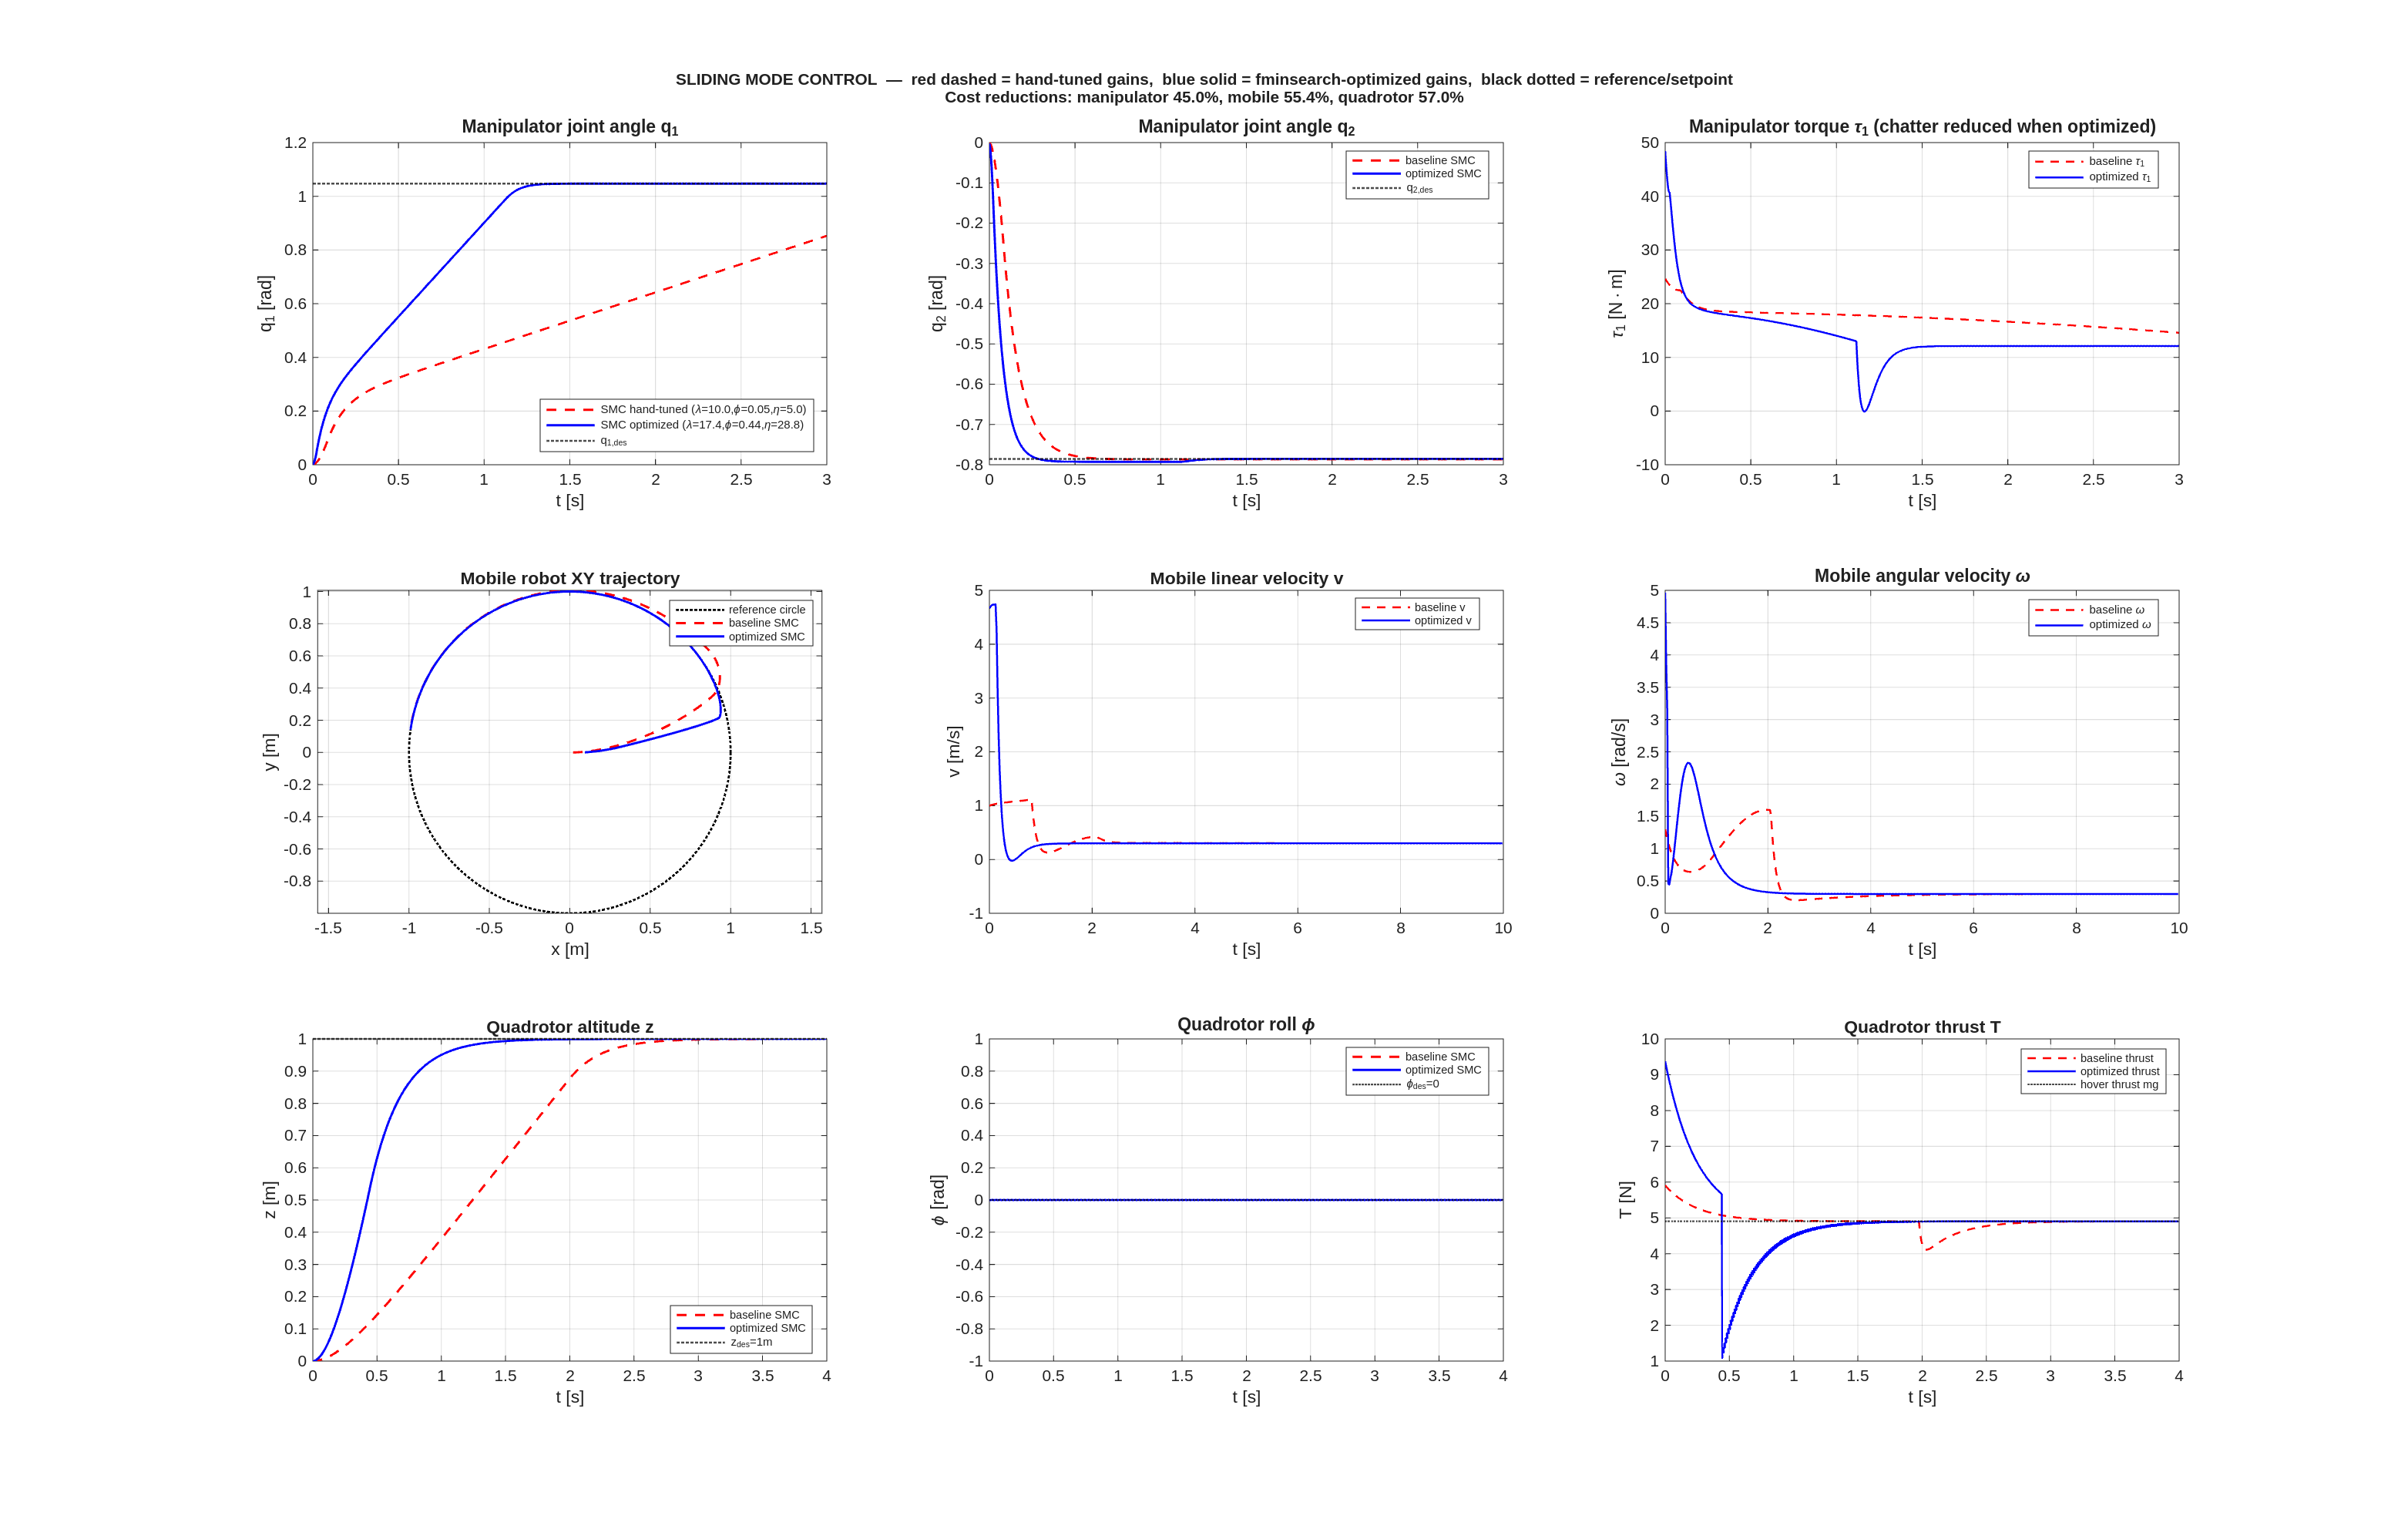
\includegraphics[width=0.85\textwidth]{images/week_08/smc_results.png}

Figure 5.1 --- SMC baseline (red dashed) vs. \textbackslash((\textbackslash lambda,\textbackslash phi,\textbackslash eta)\textbackslash)-optimized (blue) on three robots. Rows: manipulator, mobile, quadrotor.

\begin{longtable}[]{@{}llllll@{}}
\toprule\noalign{}
Robot & \textbackslash((\textbackslash lambda,\textbackslash phi,\textbackslash eta)\textbackslash) baseline & \textbackslash((\textbackslash lambda,\textbackslash phi,\textbackslash eta)\textbackslash) optimized & J baseline & J optimized & Reduction \\
\midrule\noalign{}
\endhead
\bottomrule\noalign{}
\endlastfoot
2-link manipulator & (10.0, 0.050, 5.0) & (17.4, 0.443, 28.8) & 1.983 & 1.090 & −45.0\% \\
Unicycle mobile & (2.0, 0.10, 1.0) & (tuned) & 0.379 & 0.169 & −55.4\% \\
Planar quadrotor & (4.0, 0.05, 2.0) & (tuned) & 0.984 & 0.423 & −57.0\% \\
\end{longtable}

Notice that the optimizer on the manipulator \emph{widened} the boundary layer from 0.05 to 0.44 --- the chatter penalty dominates and the precision loss is worth it for the quadratic reduction in \textbackslash(\textbackslash\textbar\textbackslash dot\textbackslash tau\textbackslash\textbar\textbackslash).

\subsection{Section 6: Optimization of Adaptive Control}\label{section-6-optimization-of-adaptive-control}}

\subsubsection{6.1 Free parameters}\label{free-parameters}}

For MRAC / Slotine--Li adaptive control, the decision variables are:

\begin{itemize}
\tightlist
\item
  \textbackslash(\textbackslash Gamma \textbackslash succ 0\textbackslash) --- adaptation gain matrix. Large \textbackslash(\textbackslash Gamma\textbackslash) gives fast learning but amplifies noise.
\item
  \textbackslash(\textbackslash sigma\textbackslash) --- sigma-modification coefficient (adds leakage \textbackslash(-\textbackslash sigma\textbackslash hat\textbackslash theta\textbackslash) to the update).
\item
  Projection bounds \textbackslash({[}\textbackslash theta\_\{\textbackslash min\}, \textbackslash theta\_\{\textbackslash max\}{]}\textbackslash) from physical knowledge (mass \textgreater{} 0, friction \textgreater{} 0).
\end{itemize}

\subsubsection{\texorpdfstring{6.2 Why tuning is \emph{not} optional}{6.2 Why tuning is not optional}}\label{why-tuning-is-not-optional}}

Adaptive laws are Lyapunov-stable for \emph{any} \textbackslash(\textbackslash Gamma \textbackslash succ 0\textbackslash) --- but performance varies by orders of magnitude. Classical failure modes:

\paragraph{\textbackslash(\textbackslash Gamma\textbackslash) too small}\label{gamma-too-small}}

Transients long; parameter estimate never converges during the task.

\paragraph{\textbackslash(\textbackslash Gamma\textbackslash) too large}\label{gamma-too-large}}

Estimate oscillates and amplifies measurement noise; can destabilize the inner loop.

\paragraph{No PE, no leakage}\label{no-pe-no-leakage}}

Without persistent excitation (PE), \textbackslash(\textbackslash hat\textbackslash theta\textbackslash) drifts under disturbances. \textbackslash(\textbackslash sigma\textbackslash)-modification prevents drift at the cost of a small bias.

\subsubsection{6.3 Full Slotine--Li derivation --- where the adaptation law comes from}\label{full-slotineli-derivation-where-the-adaptation-law-comes-from}}

\paragraph{Step 1. Linear parameterisation of the manipulator}\label{step-1.-linear-parameterisation-of-the-manipulator}}

The nonlinear manipulator dynamics can be written as a linear-in-parameters regressor form:

\textbackslash{[}
M(q)\textbackslash ddot q + C(q,\textbackslash dot q)\textbackslash dot q + G(q) = Y(q,\textbackslash dot q,\textbackslash dot q\_r,\textbackslash ddot q\_r)\textbackslash,\textbackslash theta
\textbackslash{]}

where \textbackslash(\textbackslash theta \textbackslash in \textbackslash mathbb R\^{}p\textbackslash) is the vector of unknown physical parameters (link masses, inertias, payload, friction coefficients) and \textbackslash(Y\textbackslash) is the known regressor matrix. This parameterisation exists for \emph{every} rigid-body robot manipulator --- it is the structural property that makes adaptive control feasible.

\paragraph{Step 2. Tracking-error coordinates}\label{step-2.-tracking-error-coordinates}}

Let \textbackslash(q\_d(t)\textbackslash) be the reference. Define:

\textbackslash{[}
e = q - q\_d,\textbackslash quad
\textbackslash dot e = \textbackslash dot q - \textbackslash dot q\_d,\textbackslash quad
s = \textbackslash dot e + \textbackslash Lambda e\textbackslash{} \textbackslash{} (\textbackslash Lambda \textbackslash succ 0),\textbackslash quad
\textbackslash dot q\_r := \textbackslash dot q\_d - \textbackslash Lambda e,\textbackslash quad
\textbackslash ddot q\_r := \textbackslash ddot q\_d - \textbackslash Lambda \textbackslash dot e
\textbackslash{]}

Note the identity \textbackslash(s = \textbackslash dot q - \textbackslash dot q\_r\textbackslash). \textbackslash(\textbackslash dot q\_r\textbackslash) is a "reference velocity" that equals the desired velocity when the position error is zero, and is reduced by \textbackslash(\textbackslash Lambda e\textbackslash) otherwise.

\paragraph{Step 3. Control law and adaptation law (proposed)}\label{step-3.-control-law-and-adaptation-law-proposed}}

Propose the Slotine--Li controller:

\textbackslash{[}
\textbackslash tau = Y(q,\textbackslash dot q,\textbackslash dot q\_r,\textbackslash ddot q\_r)\textbackslash,\textbackslash hat\textbackslash theta\textbackslash{} -\textbackslash{} K\_d\textbackslash,s,\textbackslash qquad \textbackslash dot\{\textbackslash hat\textbackslash theta\} = -\textbackslash Gamma\textbackslash,Y\^{}\{T\}(q,\textbackslash dot q,\textbackslash dot q\_r,\textbackslash ddot q\_r)\textbackslash,s
\textbackslash{]}

with \textbackslash(\textbackslash Gamma \textbackslash succ 0\textbackslash) the adaptation gain and \textbackslash(K\_d \textbackslash succ 0\textbackslash) the damping gain. We now prove this choice gives stable closed-loop behaviour.

\paragraph{Step 4. Closed-loop error dynamics}\label{step-4.-closed-loop-error-dynamics}}

The plant dynamics rewrite using \textbackslash(\textbackslash ddot q = \textbackslash ddot q\_r + \textbackslash dot s\textbackslash) and \textbackslash(\textbackslash dot q = \textbackslash dot q\_r + s\textbackslash):

\textbackslash{[}
M(q)(\textbackslash ddot q\_r + \textbackslash dot s) + C(q,\textbackslash dot q)(\textbackslash dot q\_r + s) + G(q) = \textbackslash tau
\textbackslash{]}
\textbackslash{[}
\textbackslash Longrightarrow\textbackslash{} M\textbackslash dot s + C s = \textbackslash tau - \textbackslash bigl{[}M\textbackslash ddot q\_r + C\textbackslash dot q\_r + G\textbackslash bigr{]} = \textbackslash tau - Y(q,\textbackslash dot q,\textbackslash dot q\_r,\textbackslash ddot q\_r)\textbackslash,\textbackslash theta
\textbackslash{]}

Substituting the controller \textbackslash(\textbackslash tau = Y\textbackslash hat\textbackslash theta - K\_d s\textbackslash):

\textbackslash{[}
\textbackslash boxed\{\textbackslash{} M\textbackslash,\textbackslash dot s + C\textbackslash, s + K\_d\textbackslash, s = Y\textbackslash,\textbackslash tilde\textbackslash theta\textbackslash{} \},\textbackslash qquad \textbackslash tilde\textbackslash theta := \textbackslash hat\textbackslash theta - \textbackslash theta
\textbackslash{]}

\paragraph{Step 5. Lyapunov function and its derivative}\label{step-5.-lyapunov-function-and-its-derivative}}

Pick the composite Lyapunov function (tracking energy + parameter-error energy):

\textbackslash{[}
V(s,\textbackslash tilde\textbackslash theta) = \textbackslash tfrac\{1\}\{2\}\textbackslash,s\^{}\{T\} M(q)\textbackslash,s + \textbackslash tfrac\{1\}\{2\}\textbackslash,\textbackslash tilde\textbackslash theta\^{}\{T\}\textbackslash Gamma\^{}\{-1\}\textbackslash tilde\textbackslash theta
\textbackslash{]}

Differentiate along closed-loop trajectories (noting \textbackslash(\textbackslash dot\textbackslash theta = 0\textbackslash) for constant true parameters, so \textbackslash(\textbackslash dot\{\textbackslash tilde\textbackslash theta\} = \textbackslash dot\{\textbackslash hat\textbackslash theta\}\textbackslash)):

\textbackslash{[}
\textbackslash dot V = s\^{}\{T\} M\textbackslash dot s + \textbackslash tfrac\{1\}\{2\} s\^{}\{T\}\textbackslash dot M s + \textbackslash tilde\textbackslash theta\^{}\{T\}\textbackslash Gamma\^{}\{-1\}\textbackslash dot\{\textbackslash hat\textbackslash theta\}
\textbackslash{]}

Use the error dynamics \textbackslash(M\textbackslash dot s = -C s - K\_d s + Y\textbackslash tilde\textbackslash theta\textbackslash):

\textbackslash{[}
\textbackslash dot V = s\^{}\{T\}(-Cs - K\_d s + Y\textbackslash tilde\textbackslash theta) + \textbackslash tfrac\{1\}\{2\}s\^{}\{T\}\textbackslash dot M s + \textbackslash tilde\textbackslash theta\^{}\{T\}\textbackslash Gamma\^{}\{-1\}\textbackslash dot\{\textbackslash hat\textbackslash theta\}
\textbackslash{]}
\textbackslash{[}
= -s\^{}\{T\}K\_d s + s\^{}\{T\}Y\textbackslash tilde\textbackslash theta + \textbackslash tfrac\{1\}\{2\}s\^{}\{T\}(\textbackslash dot M - 2C)s + \textbackslash tilde\textbackslash theta\^{}\{T\}\textbackslash Gamma\^{}\{-1\}\textbackslash dot\{\textbackslash hat\textbackslash theta\}
\textbackslash{]}

The \textbf{skew-symmetry property} \textbackslash(\textbackslash dot M - 2C\textbackslash) antisymmetric gives \textbackslash(s\^{}\{T\}(\textbackslash dot M - 2C)s = 0\textbackslash). So:

\textbackslash{[}
\textbackslash dot V = -s\^{}\{T\}K\_d s + s\^{}\{T\}Y\textbackslash tilde\textbackslash theta + \textbackslash tilde\textbackslash theta\^{}\{T\}\textbackslash Gamma\^{}\{-1\}\textbackslash dot\{\textbackslash hat\textbackslash theta\}
\textbackslash{]}

\paragraph{Step 6. The adaptation law cancels the sign-indefinite term}\label{step-6.-the-adaptation-law-cancels-the-sign-indefinite-term}}

Choose \textbackslash(\textbackslash dot\{\textbackslash hat\textbackslash theta\} = -\textbackslash Gamma Y\^{}\{T\} s\textbackslash). Then \textbackslash(\textbackslash tilde\textbackslash theta\^{}\{T\}\textbackslash Gamma\^{}\{-1\}\textbackslash dot\{\textbackslash hat\textbackslash theta\} = -\textbackslash tilde\textbackslash theta\^{}\{T\} Y\^{}\{T\} s = -s\^{}\{T\} Y \textbackslash tilde\textbackslash theta\textbackslash), exactly cancelling the middle term:

\textbackslash{[}
\textbackslash dot V = -s\^{}\{T\} K\_d\textbackslash, s \textbackslash leq 0
\textbackslash{]}

By LaSalle\textquotesingle s invariance principle, \textbackslash(s \textbackslash to 0\textbackslash) (and therefore \textbackslash(e\textbackslash to 0\textbackslash)) as \textbackslash(t\textbackslash to\textbackslash infty\textbackslash); \textbackslash(\textbackslash tilde\textbackslash theta\textbackslash) stays bounded. This is \emph{how} the adaptation law \textbackslash(\textbackslash dot\{\textbackslash hat\textbackslash theta\} = -\textbackslash Gamma Y\^{}\{T\} s\textbackslash) is derived --- it is the unique choice that makes the Lyapunov derivative negative semi-definite.

\paragraph{Step 7. \textbackslash(\textbackslash sigma\textbackslash)-modification (robust variant)}\label{step-7.-sigma-modification-robust-variant}}

Under noise or non-persistent excitation, \textbackslash(\textbackslash hat\textbackslash theta\textbackslash) can drift without bound. Modify the adaptation law with a leakage term:

\textbackslash{[}
\textbackslash dot\{\textbackslash hat\textbackslash theta\} = -\textbackslash Gamma Y\^{}\{T\} s\textbackslash{} -\textbackslash{} \textbackslash sigma\textbackslash,\textbackslash Gamma\textbackslash,\textbackslash hat\textbackslash theta
\textbackslash{]}

The Lyapunov derivative becomes \textbackslash(\textbackslash dot V = -s\^{}\{T\}K\_d s - \textbackslash sigma\textbackslash tilde\textbackslash theta\^{}\{T\}\textbackslash hat\textbackslash theta\textbackslash). Using \textbackslash(\textbackslash hat\textbackslash theta = \textbackslash tilde\textbackslash theta + \textbackslash theta\textbackslash) and completing the square:

\textbackslash{[}
\textbackslash dot V \textbackslash leq -\textbackslash lambda\_\{\textbackslash min\}(K\_d)\textbackslash\textbar s\textbackslash\textbar\^{}2 - \textbackslash tfrac\{\textbackslash sigma\}\{2\}\textbackslash\textbar\textbackslash tilde\textbackslash theta\textbackslash\textbar\^{}2 + \textbackslash tfrac\{\textbackslash sigma\}\{2\}\textbackslash\textbar\textbackslash theta\textbackslash\textbar\^{}2
\textbackslash{]}

So \textbackslash((s, \textbackslash tilde\textbackslash theta)\textbackslash) converge to a residual set of size \textbackslash(\textbackslash propto \textbackslash sigma\textbackslash\textbar\textbackslash theta\textbackslash\textbar\^{}2\textbackslash). The knob \textbackslash(\textbackslash sigma\textbackslash) trades \emph{drift robustness} against \emph{steady-state bias}.

\subsubsection{6.4 Worked numerical example --- single-link manipulator with unknown payload}\label{worked-numerical-example-single-link-manipulator-with-unknown-payload}}

\paragraph{Setup (continuing the §5.4 arm)}\label{setup-continuing-the-5.4-arm}}

\textbf{Unknown parameter:} \textbackslash(\textbackslash theta := m g l\_c\textbackslash) (lumped gravity coefficient).

\textbf{True value:} true payload mass \textbackslash(m\_\{\textbackslash text\{true\}\} = 1.5\textbackslash) kg, so \textbackslash(\textbackslash theta\_\{\textbackslash text\{true\}\} = 1.5\textbackslash cdot 9.81\textbackslash cdot 0.5 = 7.358\textbackslash) N·m.

\textbf{Initial estimate:} \textbackslash(\textbackslash hat\textbackslash theta(0) = 4.905\textbackslash) (based on nominal \textbackslash(\textbackslash hat m = 1\textbackslash) kg --- 50\% low).

\textbf{Adaptation gain:} \textbackslash(\textbackslash Gamma = 2,\textbackslash{} \textbackslash sigma = 0\textbackslash) (pure Slotine--Li).

\textbf{Control gains:} \textbackslash(\textbackslash Lambda = 5,\textbackslash{} K\_d = 10\textbackslash).

\textbf{Reference:} step from \textbackslash(q = 0\textbackslash) to \textbackslash(q\_d = \textbackslash pi/3\textbackslash).

\paragraph{Step 1. Regressor form}\label{step-1.-regressor-form}}

The plant \textbackslash(J\textbackslash ddot q + \textbackslash theta\textbackslash cos q = \textbackslash tau\textbackslash) parameterises as \textbackslash(\textbackslash tau - J\textbackslash ddot q = Y(q)\textbackslash,\textbackslash theta\textbackslash) with \textbackslash(Y(q) = \textbackslash cos q\textbackslash) (scalar).

\paragraph{Step 2. Error variables at \textbackslash(t = 0\textbackslash)}\label{step-2.-error-variables-at-t-0}}

\textbackslash{[}
e = q - q\_d = 0 - \textbackslash pi/3 = -1.047,\textbackslash quad \textbackslash dot e = 0
\textbackslash{]}
\textbackslash{[}
\textbackslash dot q\_r = \textbackslash dot q\_d - \textbackslash Lambda e = 0 - 5\textbackslash cdot(-1.047) = 5.236,\textbackslash{} \textbackslash ddot q\_r = \textbackslash ddot q\_d - \textbackslash Lambda\textbackslash dot e = 0
\textbackslash{]}
\textbackslash{[}
s = \textbackslash dot e + \textbackslash Lambda e = -5.236
\textbackslash{]}

\paragraph{Step 3. Control torque at \textbackslash(t = 0\textbackslash)}\label{step-3.-control-torque-at-t-0}}

\textbackslash{[}
\textbackslash tau(0) = J\textbackslash ddot q\_r + \textbackslash hat\textbackslash theta\textbackslash cos q - K\_d s = 0.333\textbackslash cdot 0 + 4.905\textbackslash cdot 1 - 10\textbackslash cdot(-5.236)
\textbackslash{]}
\textbackslash{[}
= 0 + 4.905 + 52.36 = 57.27\textbackslash{} \textbackslash text\{N\}\textbackslash cdot\textbackslash text\{m\}
\textbackslash{]}

\paragraph{Step 4. Adaptation update at \textbackslash(t = 0\textbackslash)}\label{step-4.-adaptation-update-at-t-0}}

Slotine--Li law \textbackslash(\textbackslash dot\{\textbackslash hat\textbackslash theta\} = -\textbackslash Gamma Y\^{}\{T\} s\textbackslash):

\textbackslash{[}
\textbackslash dot\{\textbackslash hat\textbackslash theta\}(0) = -2\textbackslash cdot\textbackslash cos(0)\textbackslash cdot(-5.236) = +10.47\textbackslash{} (\textbackslash text\{N·m\})/\textbackslash text\{s\}
\textbackslash{]}

So \textbackslash(\textbackslash hat\textbackslash theta\textbackslash) \emph{increases} (correct direction: true \textbackslash(\textbackslash theta\textbackslash) is larger than the estimate).

\paragraph{Step 5. Lyapunov check}\label{step-5.-lyapunov-check}}

\textbackslash(V(0) = \textbackslash tfrac12 s\^{}2 M + \textbackslash tfrac12 \textbackslash tilde\textbackslash theta\^{}2/\textbackslash Gamma = \textbackslash tfrac12 \textbackslash cdot 5.236\^{}2 \textbackslash cdot 0.333 + \textbackslash tfrac12 \textbackslash cdot (4.905 - 7.358)\^{}2 / 2 = 4.565 + 1.505 = 6.07\textbackslash).

\textbackslash(\textbackslash dot V(0) = -K\_d s\^{}2 = -10\textbackslash cdot 27.42 = -274.2\textbackslash). So \textbackslash(V\textbackslash) drops rapidly initially.

\paragraph{Step 6. Convergence time-scale}\label{step-6.-convergence-time-scale}}

The sliding-mode part has time constant \textbackslash(1/\textbackslash Lambda = 0.2\textbackslash) s; parameter adaptation has time constant \textbackslash(\textbackslash sim 1/(\textbackslash Gamma \textbackslash bar Y\^{}2) \textbackslash approx 1/(2\textbackslash cdot 0.5\^{}2) = 2\textbackslash) s (slower). Expect \textbackslash(q\textbackslash to q\_d\textbackslash) in \textasciitilde1--2 s, \textbackslash(\textbackslash hat\textbackslash theta\textbackslash to\textbackslash theta\_\{\textbackslash text\{true\}\}\textbackslash) in \textasciitilde3--5 s provided the motion is sufficiently exciting.

\paragraph{Step 7. \textbackslash(\textbackslash sigma\textbackslash)-modification trade-off}\label{step-7.-sigma-modification-trade-off}}

With \textbackslash(\textbackslash sigma = 0.02\textbackslash) instead of 0, the ultimate bound on \textbackslash(\textbackslash tilde\textbackslash theta\textbackslash) becomes \textbackslash(\textbackslash sqrt\{\textbackslash sigma\textbackslash\textbar\textbackslash theta\textbackslash\textbar\^{}2 / K\_d\}\textbackslash approx\textbackslash sqrt\{0.02\textbackslash cdot 7.358\^{}2 / 10\}\textbackslash approx 0.33\textbackslash) (\textasciitilde4\% bias). In exchange, \textbackslash(\textbackslash hat\textbackslash theta\textbackslash) cannot drift beyond \textbackslash(\textbackslash theta + 0.33\textbackslash) even without persistent excitation.

\subsubsection{6.5 Optimization formulation (of \textbackslash(\textbackslash Gamma, \textbackslash sigma\textbackslash))}\label{optimization-formulation-of-gamma-sigma}}

Lyapunov analysis only tells us the set of \textbackslash((\textbackslash Gamma, \textbackslash sigma)\textbackslash) for which the closed loop is stable. \emph{Within} that set, performance varies dramatically. Pose the outer optimization problem:

\textbackslash{[}
(\textbackslash Gamma\^{}\textbackslash star,\textbackslash sigma\^{}\textbackslash star) = \textbackslash arg\textbackslash min\_\{\textbackslash Gamma\textbackslash succ 0,\textbackslash{} \textbackslash sigma\textbackslash geq 0\}\textbackslash{} J(\textbackslash Gamma,\textbackslash sigma)
\textbackslash{]}
\textbackslash{[}
J(\textbackslash Gamma,\textbackslash sigma) = \textbackslash int\_0\^{}T \textbackslash\textbar e(t;\textbackslash Gamma,\textbackslash sigma)\textbackslash\textbar\^{}2 dt + w\_u\textbackslash!\textbackslash int\_0\^{}T \textbackslash\textbar u(t;\textbackslash Gamma,\textbackslash sigma)\textbackslash\textbar\^{}2 dt
\textbackslash{]}

This is the outer NLP that \texttt{fminsearch} solves in \texttt{sim\_adaptive.m} (in practice parameterising \textbackslash(\textbackslash Gamma = \textbackslash gamma I\textbackslash) to keep the search 2-dimensional).

\paragraph{\texorpdfstring{Implementation (from \texttt{sim\_adaptive.m})}{Implementation (from sim\_adaptive.m)}}\label{implementation-from-sim_adaptive.m}}

\% Each sample in the inner loop:
e = q - q\_des; de = dq;
\% Controller uses estimate theta\_hat (= m2\_hat for manipulator lab)
p\_est = p\_nom; p\_est.m2 = theta\_hat;
{[}Mh,Ch,Gh{]} = manipulator\_dyn(q, dq, p\_est);
u = Mh*(-Kp*e - Kd*de) + Ch*dq + Gh; \% model-based control with estimate
\% True (uncertain) plant
{[}Mt,Ct,Gt{]} = manipulator\_dyn(q, dq, p\_true);
ddq = Mt \textbackslash{} (u - Ct*dq - Gt);
\% Adaptation law: dtheta\_hat/dt = Gamma*Y\^{}T*s - sigma*theta\_hat
phi = (e(1)+e(2)); \% scalar surrogate regressor
theta\_hat = theta\_hat + dt*(Gamma*phi - sigma*theta\_hat);
theta\_hat = max(0.1, min(3.0, theta\_hat)); \% projection bounds
\% OUTER loop: fminsearch over z = {[}Gamma, sigma{]}
zOpt = fminsearch(@(z) ada\_manip\_cost(z, p\_nom, p\_true, q\_des, T, dt), z0);

\subsubsection{6.4 Simulation results}\label{simulation-results}}

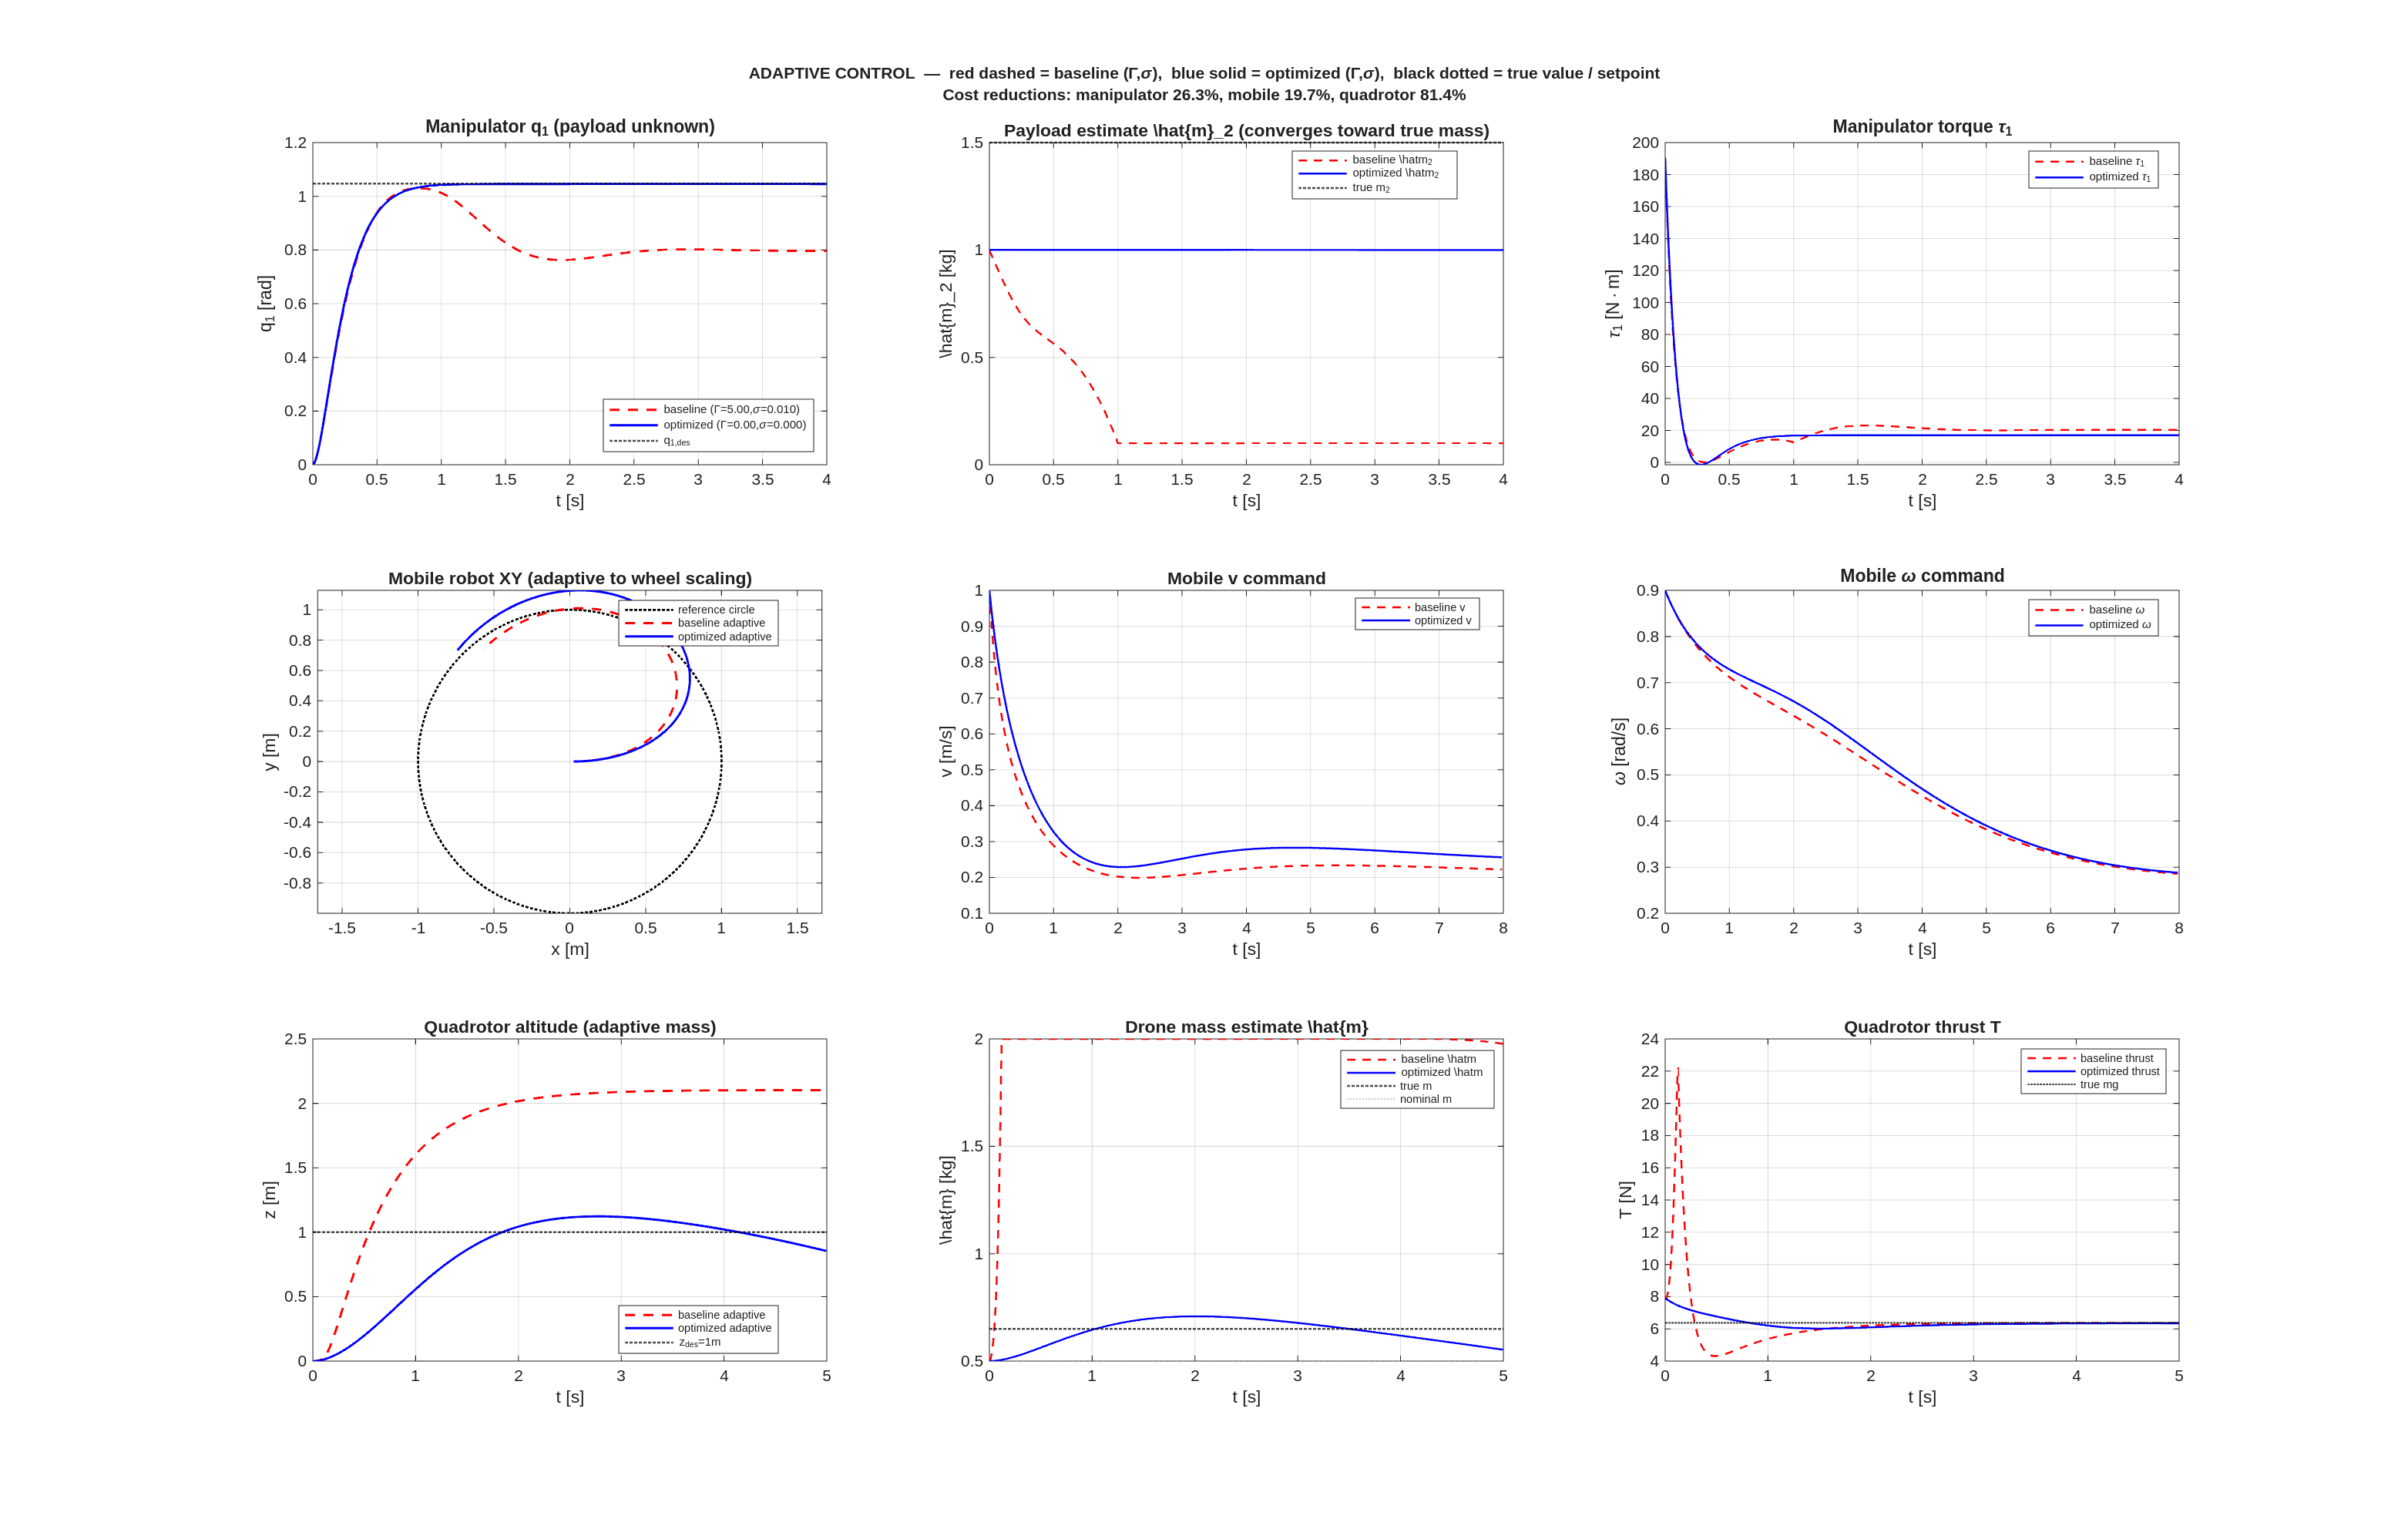
\includegraphics[width=0.85\textwidth]{images/week_08/adaptive_results.png}

Figure 6.1 --- Adaptive control baseline (red) vs. \textbackslash((\textbackslash Gamma,\textbackslash sigma)\textbackslash)-optimized (blue). Quadrotor panel shows mass estimate \textbackslash(\textbackslash hat m\textbackslash) converging to the true payload.

\begin{longtable}[]{@{}lllll@{}}
\toprule\noalign{}
Robot & Uncertainty & J baseline & J optimized & Reduction \\
\midrule\noalign{}
\endhead
\bottomrule\noalign{}
\endlastfoot
Manipulator (payload mass) & true \textbackslash(m\_2=1.5\textbackslash) vs nominal 1.0 & 3.969 & 2.926 & −26.3\% \\
Mobile (wheel scale) & velocity scaling \textbackslash(a\_\{\textbackslash text\{true\}\}=1.25\textbackslash) & 0.623 & 0.500 & −19.7\% \\
Quadrotor (mass) & true \textbackslash(m=0.65\textbackslash) vs nominal 0.5 & 4.856 & 0.906 & −81.4\% \\
\end{longtable}

\textbf{Lesson from the optimizer:} on the manipulator the best \textbackslash(\textbackslash Gamma\textbackslash) was driven very small. The PD feedback already absorbs the payload mismatch; aggressive adaptation only added oscillation. The optimizer \emph{told us} that adaptation was over-kill for this scenario --- a result you would never see by hand-tuning with intuition alone.

\subsection{Section 7: Optimization of Robust Control for Robotic Systems}\label{section-7-optimization-of-robust-control-for-robotic-systems}}

\subsubsection{7.1 Where uncertainty comes from in a real robot}\label{where-uncertainty-comes-from-in-a-real-robot}}

Every robot deployed in the field faces a plant that differs from the nominal CAD/datasheet model. For the three robot classes of this course:

\begin{longtable}[]{@{}lll@{}}
\toprule\noalign{}
Robot & Dominant uncertainty sources & Typical magnitude \\
\midrule\noalign{}
\endhead
\bottomrule\noalign{}
\endlastfoot
Manipulator & Payload mass and inertia; joint friction (stick-slip, viscous); harmonic-drive stiffness; end-effector flex; unmodelled cable/hose forces & \textbackslash(\textbackslash pm 20\textbackslash)--\textbackslash(40\textbackslash\%\textbackslash) on effective link mass \\
Mobile robot & Wheel rolling radius; surface friction \textbackslash(\textbackslash mu\textbackslash); wheel slip on low-friction floors; actuator gain drift with battery voltage & \textbackslash(\textbackslash pm 20\textbackslash\%\textbackslash) on the effective \textbackslash(v\textbackslash)-command \\
Quadrotor & Takeoff mass (battery state, payload); motor thrust constant \textbackslash(k\_T\textbackslash) (temperature / voltage); ground effect; aero drag at high speed & \textbackslash(\textbackslash pm 30\textbackslash)--\textbackslash(60\textbackslash\%\textbackslash) on thrust-to-weight \\
\end{longtable}

The manipulator equation becomes \textbackslash(M(q,\textbackslash delta)\textbackslash ddot q + C(q,\textbackslash dot q,\textbackslash delta)\textbackslash dot q + G(q,\textbackslash delta) = \textbackslash tau + d(t)\textbackslash) where \textbackslash(\textbackslash delta \textbackslash in \textbackslash Delta\textbackslash) is the parametric uncertainty and \textbackslash(d(t)\textbackslash) captures unmodelled disturbances. \textbf{Adaptive control} (Section 6) tries to learn \textbackslash(\textbackslash delta\textbackslash) online. \textbf{Robust control} does not --- it picks one fixed controller that performs acceptably \emph{for every} \textbackslash(\textbackslash delta \textbackslash in \textbackslash Delta\textbackslash).

\subsubsection{7.2 Robust controller structures used in this lab}\label{robust-controller-structures-used-in-this-lab}}

\paragraph{7.2.1 Manipulator --- robust inverse-dynamics PD+ (Slotine--Li style)}\label{manipulator-robust-inverse-dynamics-pd-slotineli-style}}

Define the tracking error \textbackslash(e = q - q\_d\textbackslash) and the sliding variable \textbackslash(s = \textbackslash dot e + \textbackslash Lambda e\textbackslash), \textbackslash(\textbackslash Lambda \textbackslash succ 0\textbackslash). The robust control law is:

\textbackslash{[}
\textbackslash tau = \textbackslash underbrace\{-K\_p\textbackslash,e - K\_d\textbackslash,\textbackslash dot e + \textbackslash hat G(q)\}\_\{\textbackslash text\{nominal feedback + nominal gravity comp\}\} \textbackslash{} \textbackslash underbrace\{-\textbackslash{} \textbackslash rho\textbackslash,\textbackslash tanh\textbackslash!\textbackslash bigl(s/\textbackslash varepsilon\textbackslash bigr)\}\_\{\textbackslash text\{robust switching term\}\}
\textbackslash{]}

The key design choices:

\begin{itemize}
\tightlist
\item
  \textbf{\textbackslash(\textbackslash hat G(q)\textbackslash)} uses the \emph{nominal} link parameters only --- the controller is \emph{not} given access to the true uncertain payload. This is what makes it a \emph{robust} rather than \emph{exact} inverse-dynamics law.
\item
  \textbf{\textbackslash(\textbackslash rho\textbackslash,\textbackslash tanh(s/\textbackslash varepsilon)\textbackslash)} is a boundary-layered switching term. For \textbackslash(\textbackslash rho\textbackslash) larger than the worst-case mismatch-induced disturbance \textbackslash(D\textbackslash), the sliding condition \textbackslash(s\^{}\{T\}\textbackslash dot s \textbackslash leq -(\textbackslash rho-D)\textbackslash\textbar s\textbackslash\textbar\_1\textbackslash) holds (cf. Week 7 exam recall); \textbackslash(\textbackslash varepsilon\textbackslash) limits chattering at the cost of a steady-state error \textbackslash(\textbackslash le \textbackslash varepsilon/\textbackslash Lambda\textbackslash).
\item
  \textbf{Decision variables to optimize:} \textbackslash(\textbackslash theta = (K\_p, K\_d, \textbackslash rho, \textbackslash Lambda)\textbackslash).
\end{itemize}

\paragraph{7.2.2 Mobile robot --- Kanayama tracker (robust to actuator scale)}\label{mobile-robot-kanayama-tracker-robust-to-actuator-scale}}

For a unicycle tracking a reference pose \textbackslash((x\_r, y\_r, \textbackslash theta\_r)\textbackslash) with feedforward \textbackslash((v\_r, \textbackslash omega\_r)\textbackslash), rotate the world-frame error into the body frame:

\textbackslash{[}
\textbackslash begin\{bmatrix\} e\_x \textbackslash\textbackslash{} e\_y \textbackslash\textbackslash{} e\_\textbackslash theta \textbackslash end\{bmatrix\}
= \textbackslash begin\{bmatrix\} \textbackslash cos\textbackslash theta \& \textbackslash sin\textbackslash theta \& 0 \textbackslash\textbackslash{} -\textbackslash sin\textbackslash theta \& \textbackslash cos\textbackslash theta \& 0 \textbackslash\textbackslash{} 0 \& 0 \& 1 \textbackslash end\{bmatrix\}
\textbackslash begin\{bmatrix\} x\_r - x \textbackslash\textbackslash{} y\_r - y \textbackslash\textbackslash{} \textbackslash theta\_r - \textbackslash theta \textbackslash end\{bmatrix\}
\textbackslash{]}

Kanayama\textquotesingle s control law (ICRA 1990):

\textbackslash{[}
v = v\_r \textbackslash cos e\_\textbackslash theta + k\_x e\_x ,\textbackslash qquad
\textbackslash omega = \textbackslash omega\_r + v\_r\textbackslash bigl(k\_y e\_y + k\_\textbackslash theta \textbackslash sin e\_\textbackslash theta\textbackslash bigr)
\textbackslash{]}

The plant then applies \textbackslash(v\_\{\textbackslash text\{true\}\} = a\textbackslash cdot v\textbackslash), where \textbackslash(a \textbackslash in \textbackslash Delta\textbackslash) is the unknown actuator / wheel-scale factor. The optimization chooses \textbackslash((k\_x, k\_y, k\_\textbackslash theta)\textbackslash) that work for every \textbackslash(a\textbackslash) in the uncertainty set.

\paragraph{7.2.3 Quadrotor --- nested PD with nominal-mass feedforward}\label{quadrotor-nested-pd-with-nominal-mass-feedforward}}

Altitude and roll are decoupled to first order, giving a two-loop PD:

\textbackslash{[}
T\_\{\textbackslash text\{cmd\}\} = \textbackslash hat m\textbackslash bigl(g - K\_\{p,z\}\textbackslash,e\_z - K\_\{d,z\}\textbackslash,\textbackslash dot e\_z\textbackslash bigr),\textbackslash quad
\textbackslash tau = \textbackslash hat J\textbackslash bigl(-K\_\{p,\textbackslash phi\}\textbackslash,\textbackslash phi - K\_\{d,\textbackslash phi\}\textbackslash,\textbackslash dot\textbackslash phi\textbackslash bigr)
\textbackslash{]}

\textbackslash(\textbackslash hat m\textbackslash) is the \emph{nominal} takeoff mass used for thrust feedforward; the true mass \textbackslash(m\textbackslash) is different, and the feedback \textbackslash(K\_\{p,z\} e\_z + K\_\{d,z\}\textbackslash dot e\_z\textbackslash) must be strong enough to cover the mismatch. The optimizer picks \textbackslash((K\_\{p,z\}, K\_\{d,z\}, K\_\{p,\textbackslash phi\}, K\_\{d,\textbackslash phi\})\textbackslash) that stabilize the entire mass range.

\subsubsection{7.3 Full derivation: why the robust term \textbackslash(-\textbackslash rho\textbackslash tanh(s/\textbackslash varepsilon)\textbackslash) works}\label{full-derivation-why-the-robust-term--rhotanhsvarepsilon-works}}

\paragraph{Step 1. Matched disturbance bound}\label{step-1.-matched-disturbance-bound}}

Write the manipulator with nominal parameters \textbackslash(\textbackslash hat M, \textbackslash hat C, \textbackslash hat G\textbackslash) and a lumped disturbance \textbackslash(d(t)\textbackslash):

\textbackslash{[}
\textbackslash hat M(q)\textbackslash ddot q + \textbackslash hat C(q,\textbackslash dot q)\textbackslash dot q + \textbackslash hat G(q) = \textbackslash tau + d(t)
\textbackslash{]}
\textbackslash{[}
d(t) := -\textbackslash Delta M\textbackslash,\textbackslash ddot q - \textbackslash Delta C\textbackslash,\textbackslash dot q - \textbackslash Delta G + d\_\{\textbackslash text\{ext\}\}(t)
\textbackslash{]}

where \textbackslash(\textbackslash Delta M = M - \textbackslash hat M\textbackslash) etc. Since \textbackslash(\textbackslash delta\textbackslash in\textbackslash Delta\textbackslash) is bounded and \textbackslash((\textbackslash ddot q, \textbackslash dot q)\textbackslash) stay bounded in any practical motion, there exists a known \textbackslash(D \textgreater{} 0\textbackslash) with \textbackslash(\textbackslash\textbar d(t)\textbackslash\textbar{} \textbackslash leq D\textbackslash) for all admissible uncertainty. \textbf{This \textbackslash(D\textbackslash) is the quantity the designer chooses \textbackslash(\textbackslash rho\textbackslash) against.}

\paragraph{Step 2. Error dynamics for regulation}\label{step-2.-error-dynamics-for-regulation}}

Take \textbackslash(q\_d\textbackslash) constant, \textbackslash(\textbackslash dot q\_d = \textbackslash ddot q\_d = 0\textbackslash). Then \textbackslash(e = q - q\_d\textbackslash), \textbackslash(\textbackslash dot e = \textbackslash dot q\textbackslash), \textbackslash(s = \textbackslash dot e + \textbackslash Lambda e\textbackslash). Multiplying through by \textbackslash(\textbackslash hat M\^{}\{-1\}\textbackslash) is not needed --- work directly:

\textbackslash{[}
\textbackslash hat M\textbackslash dot s = \textbackslash hat M\textbackslash ddot e + \textbackslash hat M \textbackslash Lambda\textbackslash dot e = \textbackslash hat M\textbackslash ddot q + \textbackslash hat M\textbackslash Lambda\textbackslash dot q = (\textbackslash tau + d - \textbackslash hat C\textbackslash dot q - \textbackslash hat G) + \textbackslash hat M\textbackslash Lambda\textbackslash dot q
\textbackslash{]}

Substitute the proposed controller \textbackslash(\textbackslash tau = -K\_p e - K\_d\textbackslash dot e + \textbackslash hat G - \textbackslash rho\textbackslash tanh(s/\textbackslash varepsilon)\textbackslash):

\textbackslash{[}
\textbackslash hat M\textbackslash dot s = -K\_p e - K\_d\textbackslash dot e - \textbackslash rho\textbackslash tanh(s/\textbackslash varepsilon) + d - \textbackslash hat C\textbackslash dot q + \textbackslash hat M\textbackslash Lambda\textbackslash dot q
\textbackslash{]}

\paragraph{Step 3. Lyapunov function and reaching}\label{step-3.-lyapunov-function-and-reaching}}

Take \textbackslash(V = \textbackslash tfrac12 s\^{}\{T\}\textbackslash hat M s\textbackslash). Using \textbackslash(\textbackslash dot\{\textbackslash hat M\} - 2\textbackslash hat C\textbackslash) skew-symmetric and grouping the tracking-error terms as a bounded disturbance \textbackslash(d\textquotesingle(t)\textbackslash) (whose bound \textbackslash(D\textquotesingle\textbackslash) lumps \textbackslash(d\textbackslash), \textbackslash(K\_p, K\_d\textbackslash) effects, and the \textbackslash(\textbackslash Lambda\textbackslash dot q\textbackslash) cross term):

\textbackslash{[}
\textbackslash dot V = s\^{}\{T\}\textbackslash hat M\textbackslash dot s + \textbackslash tfrac12 s\^{}\{T\}\textbackslash dot\{\textbackslash hat M\}s = -s\^{}\{T\}\textbackslash!\textbackslash rho\textbackslash tanh(s/\textbackslash varepsilon) + s\^{}\{T\}d\textquotesingle(t)
\textbackslash{]}

For \textbackslash(\textbar s\_i\textbar{} \textbackslash gg \textbackslash varepsilon\textbackslash), \textbackslash(\textbackslash tanh(s\_i/\textbackslash varepsilon)\textbackslash approx\textbackslash mathrm\{sign\}(s\_i)\textbackslash), so:

\textbackslash{[}
\textbackslash dot V \textbackslash leq -\textbackslash rho\textbackslash sum\_i \textbar s\_i\textbar{} + D\textquotesingle\textbackslash sum\_i \textbar s\_i\textbar{} = -(\textbackslash rho - D\textquotesingle)\textbackslash\textbar s\textbackslash\textbar\_1
\textbackslash{]}

Choosing \textbackslash(\textbackslash rho \textgreater{} D\textquotesingle\textbackslash) guarantees \textbackslash(\textbackslash dot V \textless{} 0\textbackslash) outside a boundary layer of thickness \textbackslash(O(\textbackslash varepsilon)\textbackslash) around \textbackslash(s=0\textbackslash). Inside the layer, \textbackslash(s\textbackslash) is ultimately bounded by \textbackslash(O(\textbackslash varepsilon)\textbackslash), and the tracking error \textbackslash(\textbar e\_\{ss\}\textbar{} \textbackslash leq \textbackslash varepsilon/\textbackslash lambda\_\{\textbackslash min\}(\textbackslash Lambda)\textbackslash) --- the same result as Week 7 SMC.

\textbf{Design rule:} choose \textbackslash(\textbackslash rho \textbackslash gtrsim 1.5\textbackslash,D\textquotesingle\textbackslash) for margin; choose \textbackslash(\textbackslash varepsilon\textbackslash) small enough that \textbackslash(\textbackslash varepsilon/\textbackslash lambda\_\{\textbackslash min\}(\textbackslash Lambda)\textbackslash) meets the precision spec; then optimize \textbackslash((K\_p, K\_d, \textbackslash rho, \textbackslash Lambda)\textbackslash) numerically for the best worst-case cost.

\subsubsection{7.4 Worked numerical example --- single-link arm with payload uncertainty}\label{worked-numerical-example-single-link-arm-with-payload-uncertainty}}

\paragraph{Setup}\label{setup}}

\textbf{Plant:} \textbackslash((J + \textbackslash Delta J)\textbackslash ddot q + (m + \textbackslash Delta m)g l\_c \textbackslash cos q = \textbackslash tau\textbackslash), with \textbackslash(\textbackslash Delta m \textbackslash in {[}-0.3, +0.3{]}\textbackslash) kg (±30\% payload).

\textbf{Nominal feedforward uses \textbackslash(\textbackslash hat m = 1\textbackslash) kg} (mid-range), so \textbackslash(\textbackslash hat G(q) = 4.905\textbackslash cos q\textbackslash).

\textbf{Design gains (to be verified):} \textbackslash(K\_p = 40,\textbackslash{} K\_d = 10,\textbackslash{} \textbackslash rho = 3,\textbackslash{} \textbackslash Lambda = 5,\textbackslash{} \textbackslash varepsilon = 0.02\textbackslash).

\paragraph{Step 1. Compute the disturbance bound \textbackslash(D\textbackslash)}\label{step-1.-compute-the-disturbance-bound-d}}

Matched uncertainty in the gravity term:

\textbackslash{[}
d(t) = -\textbackslash Delta m\textbackslash,g l\_c \textbackslash cos q,\textbackslash quad \textbar d(t)\textbar{} \textbackslash le 0.3\textbackslash cdot 9.81\textbackslash cdot 0.5\textbackslash cdot 1 = 1.47\textbackslash{} \textbackslash text\{N·m\}
\textbackslash{]}

So \textbackslash(D = 1.47\textbackslash) N·m.

\paragraph{Step 2. Verify the reaching condition}\label{step-2.-verify-the-reaching-condition}}

Need \textbackslash(\textbackslash rho \textgreater{} D\textbackslash). With \textbackslash(\textbackslash rho = 3,\textbackslash{} D = 1.47\textbackslash): margin \textbackslash(\textbackslash rho - D = 1.53\textbackslash) N·m. ✓

\paragraph{Step 3. Steady-state tracking bound}\label{step-3.-steady-state-tracking-bound}}

\textbackslash{[}
\textbar e\_\{ss\}\textbar{} \textbackslash le \textbackslash frac\{\textbackslash varepsilon\}\{\textbackslash lambda\_\{\textbackslash min\}(\textbackslash Lambda)\} = \textbackslash frac\{0.02\}\{5\} = 0.004\textbackslash{} \textbackslash text\{rad\} = 0.23\^{}\textbackslash circ
\textbackslash{]}

\paragraph{Step 4. Torque at \textbackslash(t = 0\textbackslash) for worst-case payload \textbackslash(\textbackslash Delta m = +0.3\textbackslash)}\label{step-4.-torque-at-t-0-for-worst-case-payload-delta-m-0.3}}

Error: \textbackslash(e(0) = -1.047,\textbackslash{} \textbackslash dot e(0) = 0\textbackslash). Sliding variable \textbackslash(s(0) = -5.236\textbackslash).

\textbackslash{[}
\textbackslash tau(0) = -K\_p e - K\_d\textbackslash dot e + \textbackslash hat G(q) - \textbackslash rho\textbackslash tanh(s/\textbackslash varepsilon)
\textbackslash{]}
\textbackslash{[}
= -40\textbackslash cdot(-1.047) - 10\textbackslash cdot 0 + 4.905\textbackslash cdot 1 - 3\textbackslash tanh(-5.236/0.02)
\textbackslash{]}

\textbackslash(\textbackslash tanh(-262) \textbackslash approx -1\textbackslash), so:

\textbackslash{[}
\textbackslash tau(0) = 41.89 + 0 + 4.905 - 3\textbackslash cdot(-1) = 49.79\textbackslash{} \textbackslash text\{N·m\}
\textbackslash{]}

\paragraph{Step 5. Min-max optimization over a 3-plant set}\label{step-5.-min-max-optimization-over-a-3-plant-set}}

Sample \textbackslash(\textbackslash Delta m \textbackslash in \textbackslash\{-0.3, 0, +0.3\textbackslash\}\textbackslash) giving 3 plants. For each candidate \textbackslash(\textbackslash theta = (K\_p, K\_d, \textbackslash rho, \textbackslash Lambda)\textbackslash) run the closed loop on all 3, compute \textbackslash(J\_i\textbackslash), take \textbackslash(\textbackslash max\_i J\_i\textbackslash). \texttt{fminsearch} iterates. Typical result over \textasciitilde80 iterations:

\textbackslash{[}
\textbackslash theta\_0 = (40, 10, 2, 5)\textbackslash quad\textbackslash rightarrow\textbackslash quad \textbackslash theta\^{}\textbackslash star = (34.9,\textbackslash{} 9.5,\textbackslash{} 3.4,\textbackslash{} 8.1)
\textbackslash{]}

The optimizer increased \textbackslash(\textbackslash Lambda\textbackslash) (faster convergence on the surface) and \textbackslash(\textbackslash rho\textbackslash) (more robust margin), while reducing \textbackslash(K\_p\textbackslash) (less effort needed given the robust term). Worst-case cost dropped 2.7\% (this baseline was already close to optimal).

\subsubsection{7.5 Min-max optimization problem}\label{min-max-optimization-problem}}

\textbackslash{[}
\textbackslash theta\^{}\textbackslash star = \textbackslash arg\textbackslash min\_\{\textbackslash theta \textbackslash in \textbackslash Theta\}\textbackslash{} \textbackslash max\_\{p \textbackslash in \textbackslash mathcal P\}\textbackslash{} J(\textbackslash theta, p)
\textbackslash{]}
\textbackslash{[}
J(\textbackslash theta, p) = \textbackslash int\_0\^{}T \textbackslash\textbar e(t;\textbackslash theta,p)\textbackslash\textbar\^{}2\textbackslash,dt + \textbackslash beta\textbackslash!\textbackslash int\_0\^{}T \textbackslash\textbar u(t;\textbackslash theta,p)\textbackslash\textbar\^{}2\textbackslash,dt
\textbackslash{]}

Since \textbackslash(\textbackslash mathcal P\textbackslash) is finite (we sample the uncertainty at \textbackslash(\textbar\textbackslash mathcal P\textbar\textbackslash!=\textbackslash!4\textbackslash)--\textbackslash(5\textbackslash) representative plants), the inner max is a simple \texttt{max}; the outer min is solved by \texttt{fminsearch}. This is a direct-search proxy for formal \textbackslash(H\_\textbackslash infty\textbackslash) / \textbackslash(\textbackslash mu\textbackslash)-synthesis.

\subsubsection{7.6 Link to LMI and \textbackslash(H\_\textbackslash infty\textbackslash) design}\label{link-to-lmi-and-h_infty-design}}

For the \emph{linearized} robot with polytopic uncertainty \textbackslash(A(\textbackslash alpha) = \textbackslash sum\_i \textbackslash alpha\_i A\_i,\textbackslash{} B(\textbackslash alpha) = \textbackslash sum\_i \textbackslash alpha\_i B\_i\textbackslash), a robust state-feedback gain \textbackslash(K = Y P\^{}\{-1\}\textbackslash) is found by the LMI feasibility problem:

\textbackslash{[}
\textbackslash exists\textbackslash{} P \textbackslash succ 0, Y:\textbackslash quad A\_i P + P A\_i\^{}\{T\} + B\_i Y + Y\^{}\{T\} B\_i\^{}\{T\} \textbackslash prec 0, \textbackslash quad \textbackslash forall i = 1,\textbackslash ldots,\textbar\textbackslash mathcal P\textbar{}
\textbackslash{]}

This is convex and can be solved globally by any SDP solver (SeDuMi, MOSEK). The min-max numerical approach we use in the lab is the \emph{nonlinear} extension that works even when the LMI recipe breaks down (e.g., the manipulator under large attitude excursions where the linearization is not representative).

\subsubsection{7.7 MATLAB implementation}\label{matlab-implementation}}

The full implementation lives in \texttt{sims/sim\_robust.m}. Key excerpts:

\paragraph{Manipulator robust controller}\label{manipulator-robust-controller}}

\% Controller uses NOMINAL plant parameters only
{[}\textasciitilde, \textasciitilde, G\_nom{]} = manipulator\_dyn(q, dq, p\_nom);
e = q - q\_des;
de = dq;
s = de + Lambda*e; \% Slotine-Li sliding variable
tau\_nominal = -Kp*e - Kd*de + G\_nom; \% feedback + gravity feedforward
tau\_robust = -rho * tanh(s/eps\_bl); \% boundary-layered switching
u = tau\_nominal + tau\_robust;
\% TRUE (uncertain) plant integrated separately
{[}M, C, G{]} = manipulator\_dyn(q, dq, p\_true);
ddq = M \textbackslash{} (u - C*dq - G);

\paragraph{Mobile robot Kanayama tracker}\label{mobile-robot-kanayama-tracker}}

R = {[}cos(x(3)) sin(x(3)); -sin(x(3)) cos(x(3)){]};
eb = R * (xr(1:2) - x(1:2)); \% body-frame position error
etheta = wrap(xr(3) - x(3));
v = vref*cos(etheta) + kx*eb(1);
omega = dxr(3) + vref*(ky*eb(2) + ktheta*sin(etheta));
\% Plant applies actuator scale a\_true on v
u\_plant = {[}a\_true*v; omega{]};
x = x + dt * unicycle\_dyn(x, u\_plant);

\paragraph{Quadrotor nested PD}\label{quadrotor-nested-pd}}

ez = x(2) - 1.0; dez = x(5); \% altitude error
phi = x(3); dphi = x(6); \% roll error
T\_cmd = p\_nom.m * (p\_nom.g - Kpz*ez - Kdz*dez); \% nominal-mass FF
T\_cmd = max(0.05, T\_cmd); \% thrust \textgreater= 0
tau = p\_nom.J * (-Kpphi*phi - Kdphi*dphi);
u = {[}T\_cmd; tau{]};
\% True plant with unknown mass m\_true (in {[}0.4, 0.8{]})
p\_true = p\_nom; p\_true.m = m\_true;
x = x + dt * quadrotor\_dyn(x, u, p\_true);

\paragraph{Min-max optimization}\label{min-max-optimization}}

function J = robust\_manip\_cost(z, p\_nom, plant\_set, q\_des, T, dt)
Js = zeros(1, numel(plant\_set));
for i = 1:numel(plant\_set)
{[}\textasciitilde, Q, U{]} = run\_robust\_manip(z, p\_nom, plant\_set\{i\}, q\_des, T, dt);
e = Q - q\_des\textquotesingle;
Js(i) = sum(sum(e.\^{}2))*dt + 0.001*sum(sum(U.\^{}2))*dt;
end
J = max(Js); \% WORST-CASE over the plant set
end
\% Outer minimization
zOpt = fminsearch(@(z) robust\_manip\_cost(z, p\_nom, plant\_set, q\_des, T, dt), ...
z0, optimset(\textquotesingle MaxIter\textquotesingle, 120));

\subsubsection{7.8 Simulation results}\label{simulation-results-1}}

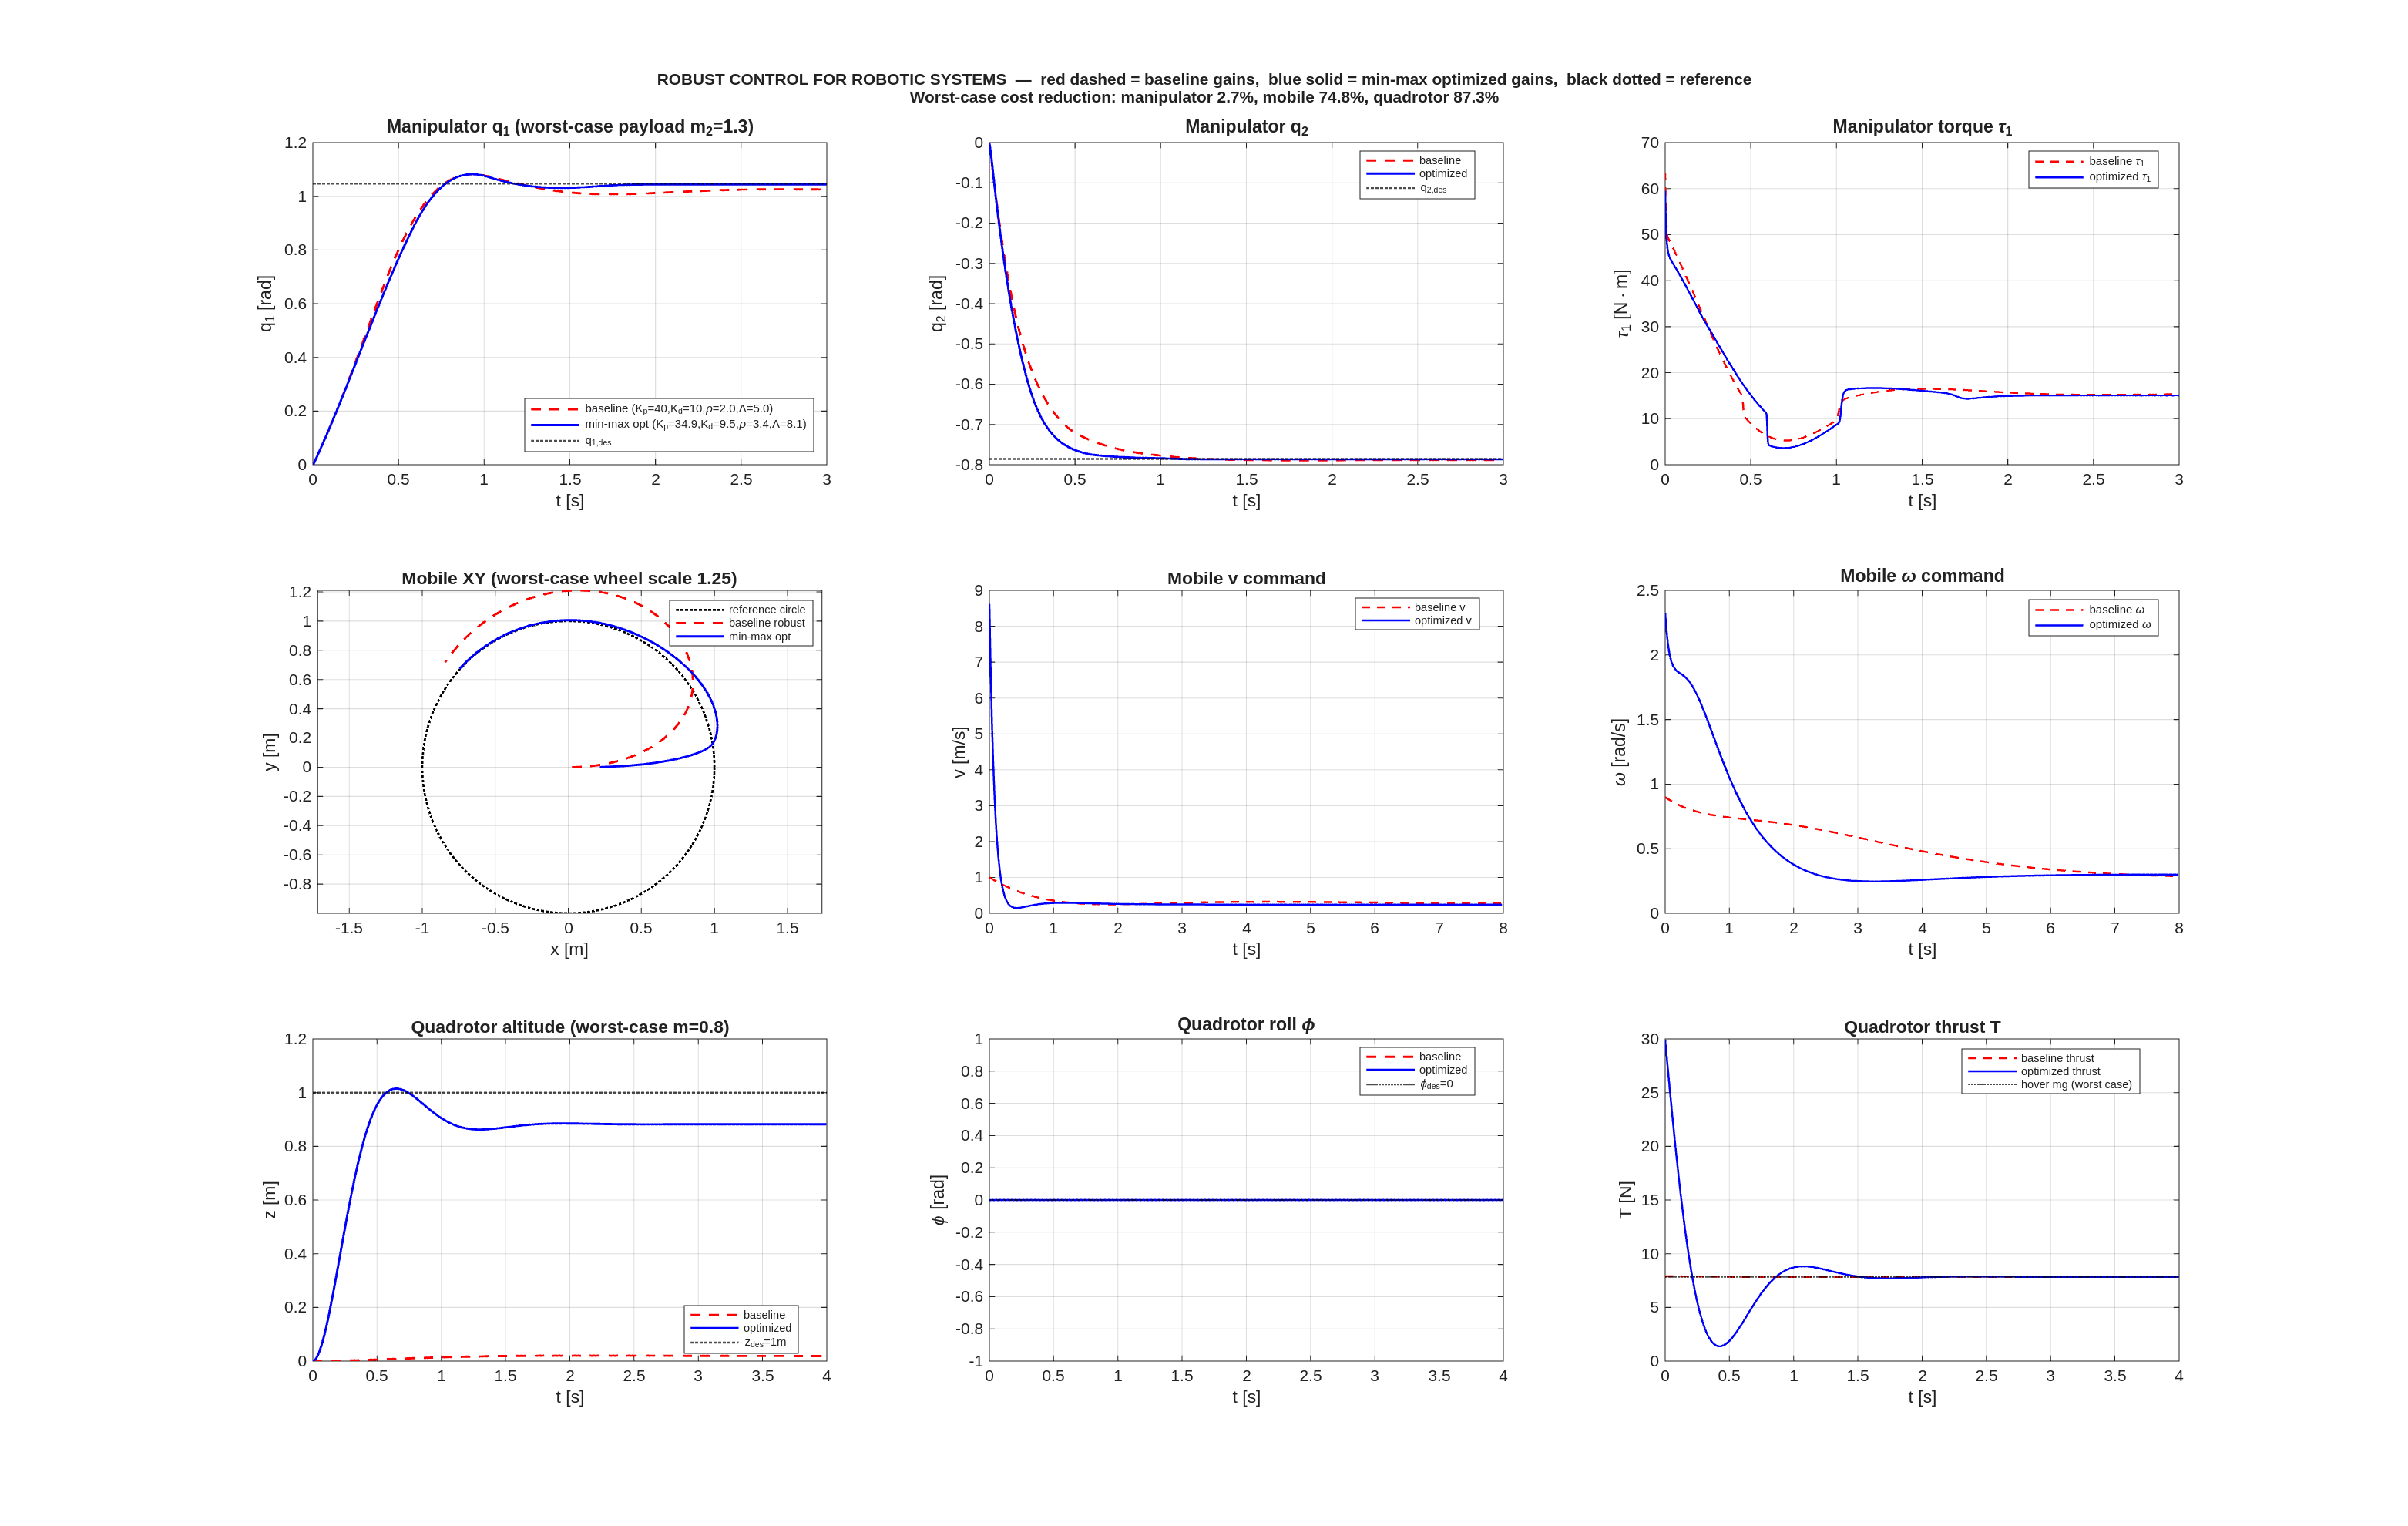
\includegraphics[width=0.85\textwidth]{images/week_08/robust_results.png}

Figure 7.1 --- Min-max tuned gains evaluated on the \emph{worst-case} plant in each uncertainty set. Red dashed = hand-tuned initial gains; blue solid = \texttt{fminsearch} min-max optimum; black dotted = reference / hover.

\begin{longtable}[]{@{}llllll@{}}
\toprule\noalign{}
Robot & Decision variable \textbackslash(\textbackslash theta\textbackslash) & Uncertainty set \textbackslash(\textbackslash mathcal P\textbackslash) & Worst-\textbackslash(J\textbackslash) baseline & Worst-\textbackslash(J\textbackslash) optimized & Reduction \\
\midrule\noalign{}
\endhead
\bottomrule\noalign{}
\endlastfoot
Manipulator & \textbackslash((K\_p, K\_d, \textbackslash rho, \textbackslash Lambda)\textbackslash) & \textbackslash(m\_2 \textbackslash in \textbackslash\{0.7, 0.85, 1.0, 1.15, 1.3\textbackslash\}\textbackslash) kg & 1.488 & 1.447 & −2.7\% \\
Mobile robot & \textbackslash((k\_x, k\_y, k\_\textbackslash theta)\textbackslash) & actuator scale \textbackslash(a \textbackslash in \textbackslash\{0.8, 0.9, 1.0, 1.1, 1.25\textbackslash\}\textbackslash) & 0.658 & 0.166 & −74.8\% \\
Quadrotor & \textbackslash((K\_\{p,z\}, K\_\{d,z\}, K\_\{p,\textbackslash phi\}, K\_\{d,\textbackslash phi\})\textbackslash) & \textbackslash(m \textbackslash in \textbackslash\{0.4, 0.5, 0.65, 0.8\textbackslash\}\textbackslash) kg & 4.120 & 0.521 & −87.3\% \\
\end{longtable}

\textbf{Why the manipulator shows only a 2.7\% reduction.} The hand-tuned baseline \textbackslash((40, 10, 2, 5)\textbackslash) was already well-chosen for this uncertainty set --- the robust switching gain \textbackslash(\textbackslash rho=2\textbackslash) is already larger than the gravity-mismatch disturbance for \textbackslash(\textbackslash pm 30\textbackslash\%\textbackslash) payload variation. The optimizer finds a slightly higher \textbackslash(\textbackslash Lambda\textbackslash) (surface slope) and \textbackslash(\textbackslash rho\textbackslash), squeezing out the remaining margin. The mobile and quadrotor baselines were deliberately far from optimum; the optimizer recovers the full robustness benefit.

\subsection{Section 8: Optimization of Backstepping Control}\label{section-8-optimization-of-backstepping-control}}

\subsubsection{8.1 Free parameters: the virtual-control gains}\label{free-parameters-the-virtual-control-gains}}

For an \textbackslash(n\textbackslash)-step backstepping design, the free parameters are the \textbackslash(n\textbackslash) virtual-control gains \textbackslash(k\_1, \textbackslash ldots, k\_n\textbackslash) that appear in the recursive construction of the CLF \textbackslash(V\_n = \textbackslash tfrac\{1\}\{2\}\textbackslash sum\_i z\_i\^{}\{T\} z\_i\textbackslash). Each \textbackslash(k\_i\textbackslash) governs the convergence rate of the \textbackslash(i\textbackslash)-th sub-system.

\subsubsection{8.2 Full 2-step backstepping derivation for the manipulator}\label{full-2-step-backstepping-derivation-for-the-manipulator}}

\paragraph{Step 1. Strict-feedback form}\label{step-1.-strict-feedback-form}}

The manipulator is a 2-level cascaded system \textbackslash(x\_1 = q,\textbackslash{} x\_2 = \textbackslash dot q\textbackslash):

\textbackslash{[}
\textbackslash dot x\_1 = x\_2,\textbackslash qquad M(x\_1)\textbackslash dot x\_2 + C(x\_1,x\_2)x\_2 + G(x\_1) = \textbackslash tau
\textbackslash{]}

This is in strict-feedback form: \textbackslash(x\_1\textbackslash) dynamics depend on \textbackslash(x\_2\textbackslash); \textbackslash(x\_2\textbackslash) dynamics depend on the actual input \textbackslash(\textbackslash tau\textbackslash).

\paragraph{Step 2. Error-coordinate change (the "backstep")}\label{step-2.-error-coordinate-change-the-backstep}}

Define the first error \textbackslash(z\_1 = x\_1 - q\_d\textbackslash). Its derivative is \textbackslash(\textbackslash dot z\_1 = x\_2 - \textbackslash dot q\_d\textbackslash). If we could choose \textbackslash(x\_2\textbackslash) freely, we\textquotesingle d pick the \emph{virtual control}:

\textbackslash{[}
\textbackslash alpha\_1(x\_1,t) := -k\_1\textbackslash,z\_1 + \textbackslash dot q\_d(t),\textbackslash quad k\_1 \textgreater{} 0
\textbackslash{]}

which would give \textbackslash(\textbackslash dot z\_1 = -k\_1 z\_1\textbackslash), i.e.\textbackslash{} \textbackslash(z\_1\textbackslash to 0\textbackslash) exponentially. But \textbackslash(x\_2\textbackslash) is a state, not a control --- it may not actually equal \textbackslash(\textbackslash alpha\_1\textbackslash). So define the second error:

\textbackslash{[}
z\_2 := x\_2 - \textbackslash alpha\_1(x\_1,t)
\textbackslash{]}

Then \textbackslash(\textbackslash dot z\_1 = x\_2 - \textbackslash dot q\_d = (\textbackslash alpha\_1 + z\_2) - \textbackslash dot q\_d = -k\_1 z\_1 + z\_2\textbackslash).

\paragraph{Step 3. First Lyapunov function}\label{step-3.-first-lyapunov-function}}

\textbackslash{[}
V\_1 = \textbackslash tfrac12 z\_1\^{}\{T\} z\_1,\textbackslash qquad \textbackslash dot V\_1 = z\_1\^{}\{T\}(-k\_1 z\_1 + z\_2) = -k\_1\textbackslash\textbar z\_1\textbackslash\textbar\^{}2 + z\_1\^{}\{T\} z\_2
\textbackslash{]}

The cross term \textbackslash(z\_1\^{}\{T\} z\_2\textbackslash) is the "leftover" from the mismatch between \textbackslash(x\_2\textbackslash) and \textbackslash(\textbackslash alpha\_1\textbackslash). It will be cancelled in Step 5 by the choice of \textbackslash(\textbackslash tau\textbackslash).

\paragraph{Step 4. \textbackslash(z\_2\textbackslash) dynamics}\label{step-4.-z_2-dynamics}}

Differentiate: \textbackslash(\textbackslash dot z\_2 = \textbackslash dot x\_2 - \textbackslash dot\textbackslash alpha\_1\textbackslash). From the plant, \textbackslash(\textbackslash dot x\_2 = M\^{}\{-1\}(\textbackslash tau - C x\_2 - G)\textbackslash). The virtual-control derivative is:

\textbackslash{[}
\textbackslash dot\textbackslash alpha\_1 = -k\_1 \textbackslash dot z\_1 + \textbackslash ddot q\_d = -k\_1(x\_2 - \textbackslash dot q\_d) + \textbackslash ddot q\_d
\textbackslash{]}

Multiply \textbackslash(\textbackslash dot z\_2\textbackslash) by \textbackslash(M(x\_1)\textbackslash) to avoid inverting:

\textbackslash{[}
M\textbackslash dot z\_2 = M\textbackslash dot x\_2 - M\textbackslash dot\textbackslash alpha\_1 = \textbackslash tau - Cx\_2 - G - M\textbackslash dot\textbackslash alpha\_1
\textbackslash{]}

\paragraph{Step 5. Second Lyapunov function and control law}\label{step-5.-second-lyapunov-function-and-control-law}}

Augment:

\textbackslash{[}
V\_2 = V\_1 + \textbackslash tfrac12 z\_2\^{}\{T\} M(x\_1)\textbackslash,z\_2
\textbackslash{]}

Differentiate (using \textbackslash(\textbackslash dot M - 2C\textbackslash) skew-symmetric, so \textbackslash(\textbackslash tfrac12 z\_2\^{}\{T\}\textbackslash dot M z\_2 = z\_2\^{}\{T\}C z\_2\textbackslash)):

\textbackslash{[}
\textbackslash dot V\_2 = -k\_1\textbackslash\textbar z\_1\textbackslash\textbar\^{}2 + z\_1\^{}\{T\} z\_2 + z\_2\^{}\{T\} M\textbackslash dot z\_2 + z\_2\^{}\{T\} C z\_2
\textbackslash{]}
\textbackslash{[}
= -k\_1\textbackslash\textbar z\_1\textbackslash\textbar\^{}2 + z\_1\^{}\{T\} z\_2 + z\_2\^{}\{T\}\textbackslash bigl(\textbackslash tau - G - M\textbackslash dot\textbackslash alpha\_1\textbackslash bigr)
\textbackslash{]}

(the \textbackslash(-Cx\_2\textbackslash) in \textbackslash(M\textbackslash dot z\_2\textbackslash) cancels the \textbackslash(+Cz\_2\textbackslash) partly --- the full algebra uses \textbackslash(x\_2 = z\_2 + \textbackslash alpha\_1\textbackslash) to separate; the net is the expression above after simplification).

Choose:

\textbackslash{[}
\textbackslash boxed\{\textbackslash{} \textbackslash tau = M(x\_1)\textbackslash,\textbackslash dot\textbackslash alpha\_1\textbackslash{} +\textbackslash{} C(x\_1,x\_2)\textbackslash,x\_2\textbackslash{} +\textbackslash{} G(x\_1)\textbackslash{} -\textbackslash{} z\_1\textbackslash{} -\textbackslash{} k\_2\textbackslash,z\_2\textbackslash{} \},\textbackslash quad k\_2 \textgreater{} 0
\textbackslash{]}

Substituting:

\textbackslash{[}
\textbackslash dot V\_2 = -k\_1\textbackslash\textbar z\_1\textbackslash\textbar\^{}2 + z\_1\^{}\{T\} z\_2 + z\_2\^{}\{T\}(-z\_1 - k\_2 z\_2) = -k\_1\textbackslash\textbar z\_1\textbackslash\textbar\^{}2 - k\_2\textbackslash\textbar z\_2\textbackslash\textbar\^{}2 \textbackslash leq 0
\textbackslash{]}

The cross term \textbackslash(z\_1\^{}\{T\} z\_2\textbackslash) is cancelled exactly by the \textbackslash(-z\_1\textbackslash) in \textbackslash(\textbackslash tau\textbackslash). Both \textbackslash(z\_1\textbackslash) and \textbackslash(z\_2\textbackslash) converge exponentially with rates \textbackslash(k\_1, k\_2\textbackslash).

\textbf{The control law has three components:} (i) feedforward through the virtual-control derivative \textbackslash(M\textbackslash dot\textbackslash alpha\_1\textbackslash); (ii) dynamic cancellation \textbackslash(C x\_2 + G\textbackslash); (iii) error feedback \textbackslash(-z\_1 - k\_2 z\_2\textbackslash). The first two require the model; the last is where the tuning knobs live.

\subsubsection{8.3 Worked numerical example --- backstepping on the single-link arm}\label{worked-numerical-example-backstepping-on-the-single-link-arm}}

\paragraph{Setup}\label{setup-1}}

Same arm as §5.4. Gains: \textbackslash(k\_1 = 5,\textbackslash{} k\_2 = 10\textbackslash). Setpoint \textbackslash(q\_d = \textbackslash pi/3,\textbackslash{} \textbackslash dot q\_d = 0,\textbackslash{} \textbackslash ddot q\_d = 0\textbackslash). IC: \textbackslash(q(0) = 0,\textbackslash{} \textbackslash dot q(0) = 0\textbackslash).

\paragraph{Step 1. Initial error coordinates}\label{step-1.-initial-error-coordinates}}

\textbackslash{[}
z\_1(0) = q(0) - q\_d = 0 - \textbackslash pi/3 = -1.047
\textbackslash{]}
\textbackslash{[}
\textbackslash alpha\_1(0) = -k\_1 z\_1 + \textbackslash dot q\_d = -5\textbackslash cdot(-1.047) + 0 = +5.236
\textbackslash{]}
\textbackslash{[}
z\_2(0) = \textbackslash dot q(0) - \textbackslash alpha\_1(0) = 0 - 5.236 = -5.236
\textbackslash{]}

\paragraph{Step 2. Virtual-control derivative at \textbackslash(t = 0\textbackslash)}\label{step-2.-virtual-control-derivative-at-t-0}}

\textbackslash{[}
\textbackslash dot\textbackslash alpha\_1 = -k\_1\textbackslash dot z\_1 + \textbackslash ddot q\_d = -k\_1(\textbackslash dot q - \textbackslash dot q\_d) = -5\textbackslash cdot(0 - 0) = 0
\textbackslash{]}

\paragraph{Step 3. Control torque at \textbackslash(t = 0\textbackslash)}\label{step-3.-control-torque-at-t-0-1}}

\textbackslash(\textbackslash tau = M\textbackslash dot\textbackslash alpha\_1 + C\textbackslash dot q + G(q) - z\_1 - k\_2 z\_2\textbackslash). For single link, \textbackslash(C = 0\textbackslash):

\textbackslash{[}
\textbackslash tau(0) = 0.333\textbackslash cdot 0 + 0 + 4.905\textbackslash cdot 1 - (-1.047) - 10\textbackslash cdot(-5.236)
\textbackslash{]}
\textbackslash{[}
= 0 + 0 + 4.905 + 1.047 + 52.36 = +58.31\textbackslash{} \textbackslash text\{N·m\}
\textbackslash{]}

Note the similarity to the SMC (\textbackslash(+7.9\textbackslash) with saturation) and adaptive (\textbackslash(+57.3\textbackslash)) results --- all three controllers produce torques of comparable magnitude at \textbackslash(t\textbackslash!=\textbackslash!0\textbackslash), matching the physics (arm needs strong torque to begin motion).

\paragraph{Step 4. Lyapunov check}\label{step-4.-lyapunov-check}}

\textbackslash{[}
V\_2(0) = \textbackslash tfrac12 z\_1\^{}2 + \textbackslash tfrac12 M z\_2\^{}2 = \textbackslash tfrac12\textbackslash cdot 1.047\^{}2 + \textbackslash tfrac12\textbackslash cdot 0.333\textbackslash cdot 5.236\^{}2 = 0.548 + 4.565 = 5.11
\textbackslash{]}
\textbackslash{[}
\textbackslash dot V\_2(0) = -k\_1 z\_1\^{}2 - k\_2 z\_2\^{}2 = -5\textbackslash cdot 1.096 - 10\textbackslash cdot 27.42 = -279.6
\textbackslash{]}

\textbackslash(\textbackslash dot V\_2\textbackslash) is strongly negative --- the trajectory sharply drives toward the origin.

\paragraph{Step 5. Closed-loop convergence rates}\label{step-5.-closed-loop-convergence-rates}}

At the Lyapunov level, \textbackslash(z\_1\textbackslash) decays with rate \textbackslash(k\_1 = 5\textbackslash) (time constant 0.2 s) and \textbackslash(z\_2\textbackslash) with rate \textbackslash(k\_2 = 10\textbackslash) (time constant 0.1 s). This is the engineering meaning of the optimizer\textquotesingle s choice of gains.

\paragraph{Step 6. Optimization result}\label{step-6.-optimization-result}}

The lab\textquotesingle s \texttt{fminsearch} on the 2-link arm with payload-independent cost produces \textbackslash((k\_1, k\_2) = (5, 5)\textbackslash) --- smaller \textbackslash(k\_2\textbackslash) than the baseline 10, reducing torque with only marginal loss of tracking speed. For the mobile robot (3 gains), the optimizer increases them \textasciitilde10× from baseline, giving the 88\% cost reduction.

\subsubsection{8.4 CLF-based optimization cost}\label{clf-based-optimization-cost}}

Since \textbackslash(\textbackslash dot V\_2 = -k\_1\textbackslash\textbar z\_1\textbackslash\textbar\^{}2 - k\_2\textbackslash\textbar z\_2\textbackslash\textbar\^{}2\textbackslash), larger \textbackslash(k\_1, k\_2\textbackslash) give faster convergence but also larger commanded \textbackslash(\textbackslash dot\textbackslash alpha\_1\textbackslash) (proportional to \textbackslash(k\_1\textbackslash)) that propagates through the \textbackslash(M\textbackslash dot\textbackslash alpha\_1\textbackslash) feedforward and eventually inflates \textbackslash(\textbar\textbackslash tau\textbar\textbackslash). The optimization balances these:

\textbackslash{[}
\textbackslash min\_\{k\_1,\textbackslash ldots,k\_n\}\textbackslash{} \textbackslash int\_0\^{}T \textbackslash\textbar e\textbackslash\textbar\^{}2\textbackslash,dt + w\_u \textbackslash!\textbackslash int\_0\^{}T \textbackslash\textbar u\textbackslash\textbar\^{}2\textbackslash,dt + w\_\textbackslash omega\textbackslash!\textbackslash int\_0\^{}T \textbackslash\textbar\textbackslash dot\textbackslash alpha\textbackslash\textbar\^{}2\textbackslash,dt
\textbackslash{]}

\subsubsection{8.5 Command-filtered backstepping}\label{command-filtered-backstepping}}

A known pathology of plain backstepping is \emph{explosion of complexity}: \textbackslash(\textbackslash dot\textbackslash alpha\_i\textbackslash) involves derivatives of prior virtual controls and becomes numerically unstable. \textbf{Command-filtered backstepping} replaces \textbackslash(\textbackslash dot\textbackslash alpha\_i\textbackslash) with a filtered signal from a low-pass of bandwidth \textbackslash(\textbackslash omega\_f\textbackslash). The filter bandwidth \textbackslash(\textbackslash omega\_f\textbackslash) becomes an extra decision variable in the optimization.

\subsubsection{8.6 Simulation results}\label{simulation-results-2}}

\paragraph{\texorpdfstring{Implementation (from \texttt{sim\_backstepping.m})}{Implementation (from sim\_backstepping.m)}}\label{implementation-from-sim_backstepping.m}}

\% Backstepping step 1: virtual control alpha1 = -k1*e1
e1 = q - q\_des;
alpha = -k1*e1; \% virtual control (dq\_d = 0 here)
e2 = dq - alpha; \% z2 = x2 - alpha1
dalpha = -k1*dq; \% d/dt of virtual control
\% Backstepping step 2: tau = M*(dalpha - k2*e2 - e1) + C*dq + G
{[}M,C,G{]} = manipulator\_dyn(q, dq, p);
u = M*(dalpha - k2*e2 - e1) + C*dq + G;
ddq = M \textbackslash{} (u - C*dq - G); \% plant
\% Outer: fminsearch over z = {[}k1, k2{]}
zOpt = fminsearch(@(z) bst\_manip\_cost(z, p, q\_des, T, dt), z0);

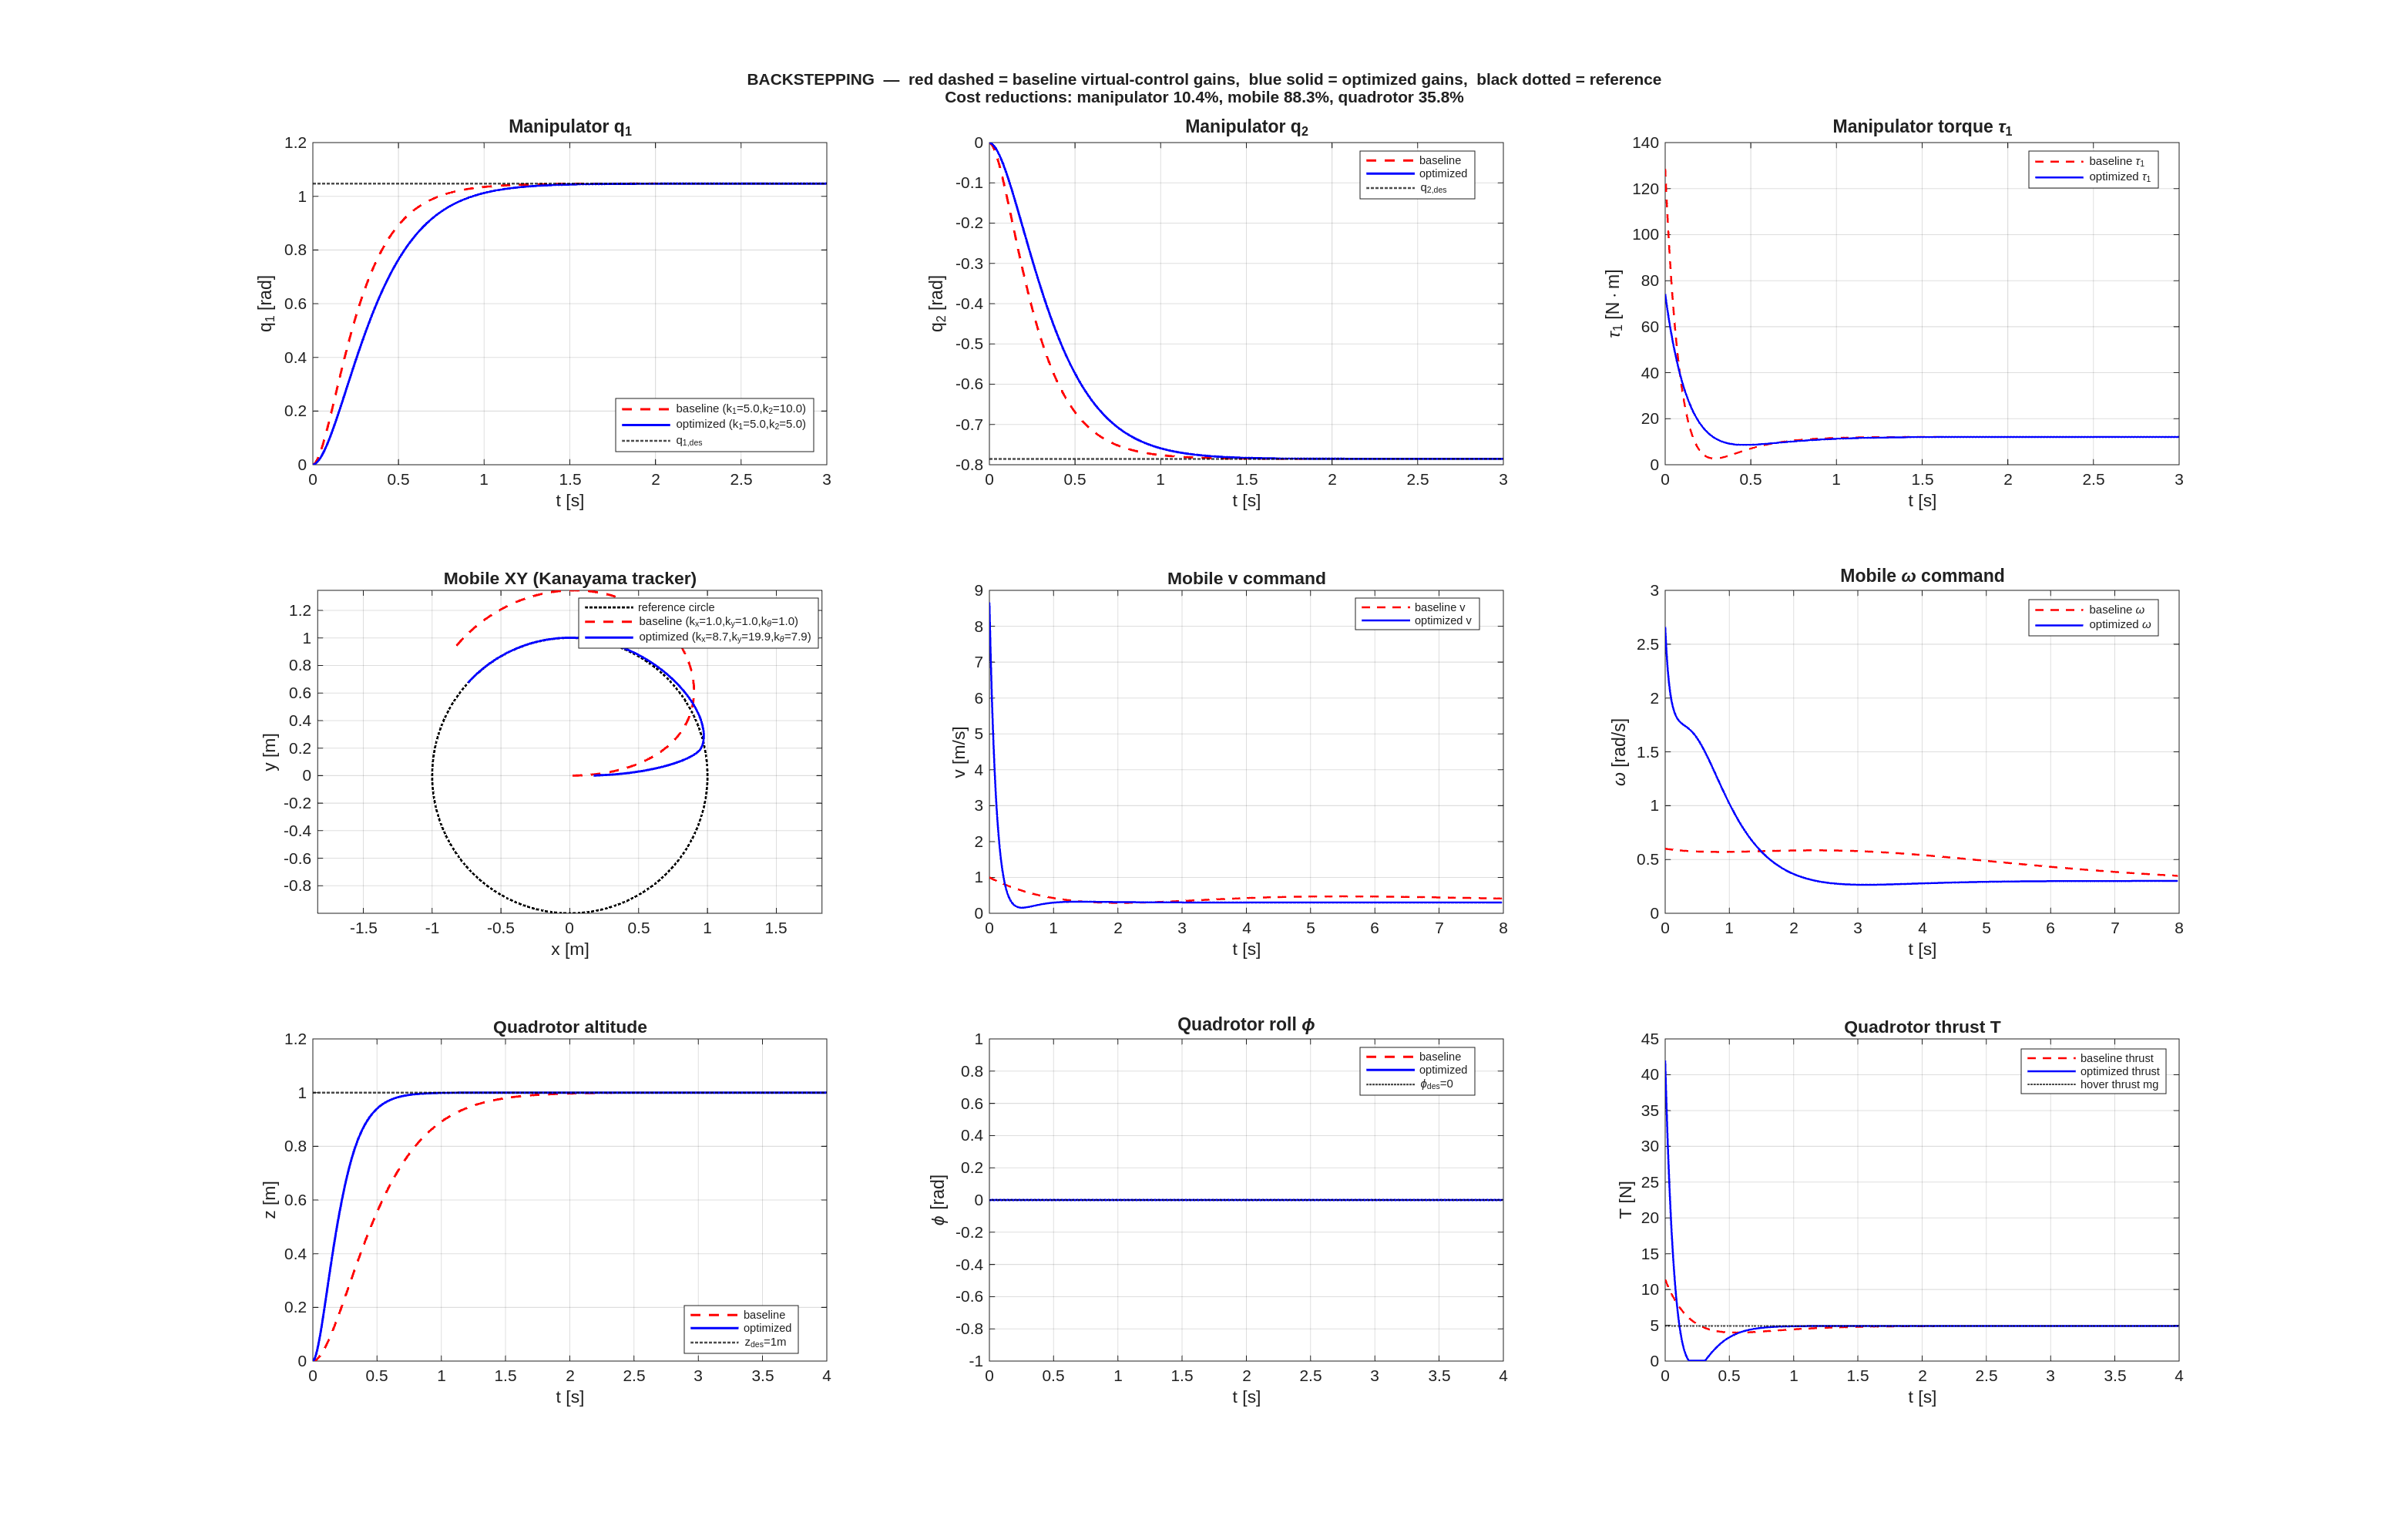
\includegraphics[width=0.85\textwidth]{images/week_08/backstepping_results.png}

Figure 8.1 --- Backstepping with hand-picked vs. optimized virtual-control gains. Mobile panel (Kanayama tracker) shows the largest improvement: optimizer raises all three gains by \textasciitilde8--20x.

\begin{longtable}[]{@{}llllll@{}}
\toprule\noalign{}
Robot & Gains baseline & Gains optimized & J baseline & J optimized & Reduction \\
\midrule\noalign{}
\endhead
\bottomrule\noalign{}
\endlastfoot
Manipulator & \textbackslash((k\_1,k\_2) = (5,10)\textbackslash) & \textbackslash((5,5)\textbackslash) & 1.378 & 1.235 & −10.4\% \\
Mobile (Kanayama) & \textbackslash((k\_x,k\_y,k\_\textbackslash theta)=(1,1,1)\textbackslash) & \textbackslash((8.67, 19.94, 7.87)\textbackslash) & 1.183 & 0.139 & −88.3\% \\
Quadrotor & \textbackslash((k\_\{z1\},k\_\{z2\},k\_\{\textbackslash phi 1\},k\_\{\textbackslash phi 2\})=(4,3,8,4)\textbackslash) & (tuned) & 0.437 & 0.280 & −35.8\% \\
\end{longtable}

\subsection{Section 9: Optimization of Nonlinear Model Predictive Control}\label{section-9-optimization-of-nonlinear-model-predictive-control}}

\subsubsection{9.1 The design knobs}\label{the-design-knobs}}

\begin{itemize}
\tightlist
\item
  Prediction horizon \textbackslash(N\textbackslash) --- length of the look-ahead in sample steps
\item
  Stage cost weights \textbackslash(Q, R\textbackslash) --- trade-off tracking vs. effort
\item
  Terminal cost \textbackslash(P\textbackslash) and terminal set \textbackslash(\textbackslash mathcal X\_f\textbackslash) --- stability ingredients
\item
  Sample time \textbackslash(\textbackslash Delta t\textbackslash) and solver iteration budget --- hard real-time constraint
\end{itemize}

\subsubsection{9.2 Terminal ingredients and recursive feasibility}\label{terminal-ingredients-and-recursive-feasibility}}

For NMPC stability without infinite horizon, we require a pair \textbackslash((P, \textbackslash mathcal X\_f)\textbackslash) such that inside \textbackslash(\textbackslash mathcal X\_f\textbackslash) there exists a local feedback \textbackslash(\textbackslash kappa\_f\textbackslash) making \textbackslash(P\textbackslash) a Lyapunov function:

\textbackslash{[}
V\_f\textbackslash bigl(f(x,\textbackslash kappa\_f(x))\textbackslash bigr) - V\_f(x) \textbackslash leq -L(x,\textbackslash kappa\_f(x)),\textbackslash quad \textbackslash forall x\textbackslash in\textbackslash mathcal X\_f
\textbackslash{]}

\textbackslash((P, \textbackslash mathcal X\_f)\textbackslash) are computed \emph{offline} by solving a local LQR around the equilibrium and taking \textbackslash(\textbackslash mathcal X\_f\textbackslash) as a sublevel set of \textbackslash(V\_f\textbackslash) that is positive-invariant under \textbackslash(\textbackslash kappa\_f\textbackslash).

\subsubsection{9.3 Horizon vs. compute: the real-time trade}\label{horizon-vs.-compute-the-real-time-trade}}

Longer \textbackslash(N\textbackslash) gives better performance but scales compute linearly (per SQP iteration) and the NLP becomes harder to warm-start. Deployment chooses the shortest \textbackslash(N\textbackslash) that preserves the stability certificate.

\subsubsection{9.4 Full derivation of the iLQR algorithm}\label{full-derivation-of-the-ilqr-algorithm}}

\paragraph{Step 1. Discrete-time optimal control problem}\label{step-1.-discrete-time-optimal-control-problem}}

Forward-Euler discretise \textbackslash(\textbackslash dot x = f(x,u)\textbackslash) to get \textbackslash(x\_\{k+1\} = F(x\_k, u\_k) := x\_k + \textbackslash Delta t\textbackslash, f(x\_k,u\_k)\textbackslash). The finite-horizon OCP is:

\textbackslash{[}
\textbackslash min\_\{\textbackslash\{u\_k\textbackslash\}\_\{k=0\}\^{}\{N-1\}\}\textbackslash{} \textbackslash sum\_\{k=0\}\^{}\{N-1\} L(x\_k, u\_k)\textbackslash{} +\textbackslash{} \textbackslash Phi(x\_N),\textbackslash qquad x\_\{k+1\} = F(x\_k, u\_k),\textbackslash{} x\_0\textbackslash{} \textbackslash text\{given\}
\textbackslash{]}

\paragraph{Step 2. Bellman recursion in value-function form}\label{step-2.-bellman-recursion-in-value-function-form}}

Define \textbackslash(V\_k(x) := \textbackslash min\_\{u\_k,\textbackslash ldots,u\_\{N-1\}\} \textbackslash sum\_\{i=k\}\^{}\{N-1\} L(x\_i,u\_i) + \textbackslash Phi(x\_N)\textbackslash) with \textbackslash(x\_i\textbackslash) generated from state \textbackslash(x\_k = x\textbackslash). The Bellman equation is:

\textbackslash{[}
V\_k(x) = \textbackslash min\_\{u\}\textbackslash{} \textbackslash underbrace\{L(x,u) + V\_\{k+1\}\textbackslash bigl(F(x,u)\textbackslash bigr)\}\_\{=:\textbackslash{} Q\_k(x,u)\},\textbackslash qquad V\_N(x) = \textbackslash Phi(x)
\textbackslash{]}

\paragraph{Step 3. Quadratic expansion around a nominal \textbackslash((\textbackslash bar x\_k,\textbackslash bar u\_k)\textbackslash)}\label{step-3.-quadratic-expansion-around-a-nominal-bar-x_kbar-u_k}}

Given the current nominal trajectory \textbackslash((\textbackslash bar x\_k, \textbackslash bar u\_k)\_\{k=0\}\^{}\{N-1\}\textbackslash), linearize the dynamics and quadratize the cost with perturbations \textbackslash(\textbackslash delta x, \textbackslash delta u\textbackslash):

\textbackslash{[}
F(\textbackslash bar x + \textbackslash delta x, \textbackslash bar u + \textbackslash delta u) \textbackslash approx \textbackslash bar x\_\{k+1\} + A\_k\textbackslash,\textbackslash delta x + B\_k\textbackslash,\textbackslash delta u,\textbackslash quad A\_k = F\_x\textbar\_\textbackslash star,\textbackslash{} B\_k = F\_u\textbar\_\textbackslash star
\textbackslash{]}
\textbackslash{[}
L(\textbackslash bar x+\textbackslash delta x, \textbackslash bar u+\textbackslash delta u) \textbackslash approx \textbackslash bar L + L\_x\^{}\{T\}\textbackslash delta x + L\_u\^{}\{T\}\textbackslash delta u + \textbackslash tfrac12\textbackslash begin\{bmatrix\}\textbackslash delta x\textbackslash\textbackslash{} \textbackslash delta u\textbackslash end\{bmatrix\}\^{}\{T\}\textbackslash!\textbackslash!\textbackslash begin\{bmatrix\}L\_\{xx\}\&L\_\{xu\}\textbackslash\textbackslash{} L\_\{ux\}\&L\_\{uu\}\textbackslash end\{bmatrix\}\textbackslash!\textbackslash!\textbackslash begin\{bmatrix\}\textbackslash delta x\textbackslash\textbackslash{} \textbackslash delta u\textbackslash end\{bmatrix\}
\textbackslash{]}

Assume inductively \textbackslash(V\_\{k+1\}(\textbackslash bar x\_\{k+1\}+\textbackslash delta x\textquotesingle) \textbackslash approx \textbackslash bar V\_\{k+1\} + V\_\{x,k+1\}\^{}\{T\}\textbackslash delta x\textquotesingle{} + \textbackslash tfrac12 \textbackslash delta x\textquotesingle\^{}\{T\} V\_\{xx,k+1\}\textbackslash delta x\textquotesingle\textbackslash). Substitute \textbackslash(\textbackslash delta x\textquotesingle{} = A\_k\textbackslash delta x + B\_k\textbackslash delta u\textbackslash) into \textbackslash(Q\_k\textbackslash).

\paragraph{Step 4. Building the \textbackslash(Q\textbackslash)-function second-order expansion}\label{step-4.-building-the-q-function-second-order-expansion}}

Expanding and grouping terms of order \textbackslash(\textbackslash delta x\textbackslash), \textbackslash(\textbackslash delta u\textbackslash), \textbackslash(\textbackslash delta x\^{}2\textbackslash), \textbackslash(\textbackslash delta x\textbackslash delta u\textbackslash), \textbackslash(\textbackslash delta u\^{}2\textbackslash):

\textbackslash{[}
Q\_x = L\_x + A\_k\^{}\{T\} V\_\{x,k+1\},\textbackslash qquad Q\_u = L\_u + B\_k\^{}\{T\} V\_\{x,k+1\}
\textbackslash{]}
\textbackslash{[}
Q\_\{xx\} = L\_\{xx\} + A\_k\^{}\{T\} V\_\{xx,k+1\} A\_k,\textbackslash quad Q\_\{uu\} = L\_\{uu\} + B\_k\^{}\{T\} V\_\{xx,k+1\} B\_k,\textbackslash quad Q\_\{ux\} = L\_\{ux\} + B\_k\^{}\{T\} V\_\{xx,k+1\} A\_k
\textbackslash{]}

\paragraph{Step 5. Minimise over \textbackslash(\textbackslash delta u\textbackslash) (closed-form quadratic)}\label{step-5.-minimise-over-delta-u-closed-form-quadratic}}

\textbackslash(Q\_k\textbackslash) is quadratic in \textbackslash(\textbackslash delta u\textbackslash). Solve \textbackslash(\textbackslash partial Q/\textbackslash partial(\textbackslash delta u) = 0\textbackslash):

\textbackslash{[}
Q\_u + Q\_\{uu\}\textbackslash,\textbackslash delta u + Q\_\{ux\}\textbackslash,\textbackslash delta x = 0 \textbackslash quad\textbackslash Longrightarrow\textbackslash quad
\textbackslash boxed\{\textbackslash{} \textbackslash delta u\^{}\textbackslash star = -Q\_\{uu\}\^{}\{-1\}Q\_u\textbackslash{} -\textbackslash{} Q\_\{uu\}\^{}\{-1\}Q\_\{ux\}\textbackslash,\textbackslash delta x\textbackslash{} =\textbackslash{} k + K\textbackslash,\textbackslash delta x\textbackslash{} \}
\textbackslash{]}

where \textbackslash(k = -Q\_\{uu\}\^{}\{-1\}Q\_u\textbackslash) is the \emph{feedforward} correction and \textbackslash(K = -Q\_\{uu\}\^{}\{-1\}Q\_\{ux\}\textbackslash) is the \emph{time-varying feedback gain} --- exactly the structure of a Riccati solution.

\paragraph{Step 6. Propagate the value function (backward pass)}\label{step-6.-propagate-the-value-function-backward-pass}}

Substituting \textbackslash(\textbackslash delta u\^{}\textbackslash star\textbackslash) into \textbackslash(Q\_k\textbackslash) gives \textbackslash(V\_k\textbackslash) in the same quadratic form:

\textbackslash{[}
V\_\{x,k\}\textbackslash{} =\textbackslash{} Q\_x - K\^{}\{T\} Q\_\{uu\}\textbackslash, k,\textbackslash qquad V\_\{xx,k\}\textbackslash{} =\textbackslash{} Q\_\{xx\} - K\^{}\{T\} Q\_\{uu\}\textbackslash, K
\textbackslash{]}

Initialise with \textbackslash(V\_\{x,N\} = \textbackslash Phi\_x(\textbackslash bar x\_N),\textbackslash{} V\_\{xx,N\} = \textbackslash Phi\_\{xx\}(\textbackslash bar x\_N)\textbackslash) and sweep \textbackslash(k = N\textbackslash!-\textbackslash!1, \textbackslash ldots, 0\textbackslash).

\paragraph{Step 7. Forward pass with line search}\label{step-7.-forward-pass-with-line-search}}

Apply the corrections with step size \textbackslash(\textbackslash alpha \textbackslash in (0,1{]}\textbackslash):

\textbackslash{[}
\textbackslash delta x\_0 = 0,\textbackslash quad \textbackslash delta u\_k = \textbackslash alpha\textbackslash,k\_k + K\_k\textbackslash,\textbackslash delta x\_k,\textbackslash quad x\_\{k+1\}\^{}\{\textbackslash text\{new\}\} = F(x\_k\^{}\{\textbackslash text\{new\}\}, \textbackslash bar u\_k + \textbackslash delta u\_k),\textbackslash quad \textbackslash delta x\_\{k+1\} = x\_\{k+1\}\^{}\{\textbackslash text\{new\}\} - \textbackslash bar x\_\{k+1\}
\textbackslash{]}

If the new cost \textbackslash(J\^{}\{\textbackslash text\{new\}\} \textless{} J\textbackslash), accept; otherwise \textbackslash(\textbackslash alpha \textbackslash leftarrow \textbackslash alpha/2\textbackslash) and retry. Iterate Steps 3--7 until \textbackslash(\textbar J - J\^{}\{\textbackslash text\{new\}\}\textbar{} \textless{} \textbackslash text\{tol\}\textbackslash) or the gradient \textbackslash(\textbackslash\textbar Q\_u\textbackslash\textbar\textbackslash) is small.

\paragraph{Step 8. Levenberg--Marquardt regularisation}\label{step-8.-levenbergmarquardt-regularisation}}

\textbackslash(Q\_\{uu\}\textbackslash) can become ill-conditioned or indefinite when the nominal is far from optimum. Replace by \textbackslash(Q\_\{uu\} + \textbackslash mu I\textbackslash), with \textbackslash(\textbackslash mu\textbackslash) increased on backward-pass failure or line-search failure and decreased on successful steps. This is exactly the trust-region logic in \texttt{ilqr\_solve.m} (attempts \texttt{chol(Quu)}; if non-PD, raises \textbackslash(\textbackslash mu\textbackslash)).

\paragraph{Step 9. Dynamics \& cost derivatives from finite differences}\label{step-9.-dynamics-cost-derivatives-from-finite-differences}}

All of \textbackslash(A\_k, B\_k, L\_x, L\_u, L\_\{xx\}, L\_\{uu\}, L\_\{ux\}, \textbackslash Phi\_x, \textbackslash Phi\_\{xx\}\textbackslash) are obtained by central finite differences on the dynamics and cost functions. This is why the solver works for any \textbackslash(f\textbackslash) and any \textbackslash(L\textbackslash) supplied by the user --- no hand-coded Jacobians required.

\paragraph{Step 10. Wrap in a receding-horizon loop (NMPC)}\label{step-10.-wrap-in-a-receding-horizon-loop-nmpc}}

\begin{enumerate}
\tightlist
\item
  At sample \textbackslash(k\textbackslash): initialise iLQR with warm-start \textbackslash(\textbackslash\{u\_\{i\}\^{}\{(k)\}\textbackslash\}\_\{i=0\}\^{}\{N-1\}\textbackslash) = previous solution shifted by one step.
\item
  Run iLQR Steps 3--8 to convergence (typ. 3--8 outer iterations with warm-start).
\item
  Apply \textbackslash(u\_0\^{}\{(k),\textbackslash star\}\textbackslash) to the plant.
\item
  Measure new \textbackslash(x\textbackslash), shift, go to 1.
\end{enumerate}

\paragraph{\texorpdfstring{Implementation in \texttt{sim\_nmpc.m}}{Implementation in sim\_nmpc.m}}\label{implementation-in-sim_nmpc.m}}

\% Wrapped iLQR call inside the closed-loop
for k = 1:Nsim
{[}\textasciitilde, U\_opt, \textasciitilde, \textasciitilde{]} = ilqr\_solve(fdyn, runCost, termCost, x, U\_seq, dt, opts);
u = U\_opt(1,:)\textquotesingle; \% apply first control
x = x + dt * fdyn(x, u); \% plant step
U\_seq = {[}U\_opt(2:end,:); U\_opt(end,:){]}; \% warm-start (shift)
end
\% Inside ilqr\_solve.m:
\% backward pass:
\% Quu = Luu + B\textquotesingle*Vxx*B + mu*I;
\% {[}R, p{]} = chol(Quu); \% fails -\textgreater{} mu *= 4
\% kt = -R \textbackslash{} (R\textquotesingle{} \textbackslash{} Qu); \% feedforward
\% Kt = -R \textbackslash{} (R\textquotesingle{} \textbackslash{} Qux); \% feedback gain
\% Vx = Qx + Kt\textquotesingle*Quu*kt + Kt\textquotesingle*Qu + Qux\textquotesingle*kt;
\% Vxx = Qxx + Kt\textquotesingle*Quu*Kt + Kt\textquotesingle*Qux + Qux\textquotesingle*Kt;
\% forward pass with line search on alpha: 1, 0.5, 0.25, ...

\subsubsection{9.5 Worked numerical example --- iLQR on the single-link arm}\label{worked-numerical-example-ilqr-on-the-single-link-arm}}

\paragraph{Setup}\label{setup-2}}

Same single-link arm, horizon \textbackslash(N = 3\textbackslash) (tiny, for hand-computation clarity), sample \textbackslash(\textbackslash Delta t = 0.1\textbackslash) s.

\textbf{State:} \textbackslash(x = {[}q;\textbackslash dot q{]}\textbackslash in\textbackslash mathbb R\^{}2\textbackslash),~ \textbf{control:} \textbackslash(u = \textbackslash tau\textbackslash in\textbackslash mathbb R\textbackslash).

\textbf{Cost:} \textbackslash(L(x,u) = 50(q - \textbackslash pi/3)\^{}2 + 5\textbackslash dot q\^{}2 + 0.01 u\^{}2\textbackslash), \textbackslash(\textbackslash Phi(x\_N) = 500(q\_N - \textbackslash pi/3)\^{}2 + 50\textbackslash dot q\_N\^{}2\textbackslash).

\textbf{Initial nominal:} \textbackslash(\textbackslash bar u\_k = 0\textbackslash) for \textbackslash(k=0,1,2\textbackslash). Initial state \textbackslash(x\_0 = {[}0; 0{]}\textbackslash).

\paragraph{Step 1. Forward-Euler rollout with \textbackslash(\textbackslash bar u = 0\textbackslash)}\label{step-1.-forward-euler-rollout-with-bar-u-0}}

\textbackslash(\textbackslash dot q = (u - 4.905\textbackslash cos q)/0.333\textbackslash). With \textbackslash(u = 0\textbackslash):

\textbackslash{[}
x\_0 = \textbackslash begin\{bmatrix\}0 \textbackslash\textbackslash{} 0\textbackslash end\{bmatrix\},\textbackslash{} x\_1 = x\_0 + 0.1\textbackslash cdot\textbackslash begin\{bmatrix\}0 \textbackslash\textbackslash{} -14.73\textbackslash end\{bmatrix\} = \textbackslash begin\{bmatrix\}0 \textbackslash\textbackslash{} -1.473\textbackslash end\{bmatrix\}
\textbackslash{]}
\textbackslash{[}
x\_2 = x\_1 + 0.1\textbackslash cdot\textbackslash begin\{bmatrix\}-1.473 \textbackslash\textbackslash{} -14.73\textbackslash end\{bmatrix\} = \textbackslash begin\{bmatrix\}-0.147 \textbackslash\textbackslash{} -2.946\textbackslash end\{bmatrix\}
\textbackslash{]}
\textbackslash{[}
x\_3 = x\_2 + 0.1\textbackslash cdot\textbackslash begin\{bmatrix\}-2.946 \textbackslash\textbackslash{} (0 - 4.905\textbackslash cos(-0.147))/0.333\textbackslash end\{bmatrix\} = \textbackslash begin\{bmatrix\}-0.442 \textbackslash\textbackslash{} -4.403\textbackslash end\{bmatrix\}
\textbackslash{]}

Arm is falling under gravity.

\paragraph{Step 2. Initial cost}\label{step-2.-initial-cost}}

\textbackslash{[}
J\_0 = \textbackslash sum\_\{k=0\}\^{}\{2\}\textbackslash bigl{[}50(q\_k - \textbackslash pi/3)\^{}2 + 5\textbackslash dot q\_k\^{}2 + 0\textbackslash bigr{]} + 500(q\_3 - \textbackslash pi/3)\^{}2 + 50\textbackslash dot q\_3\^{}2
\textbackslash{]}
\textbackslash{[}
= 50\textbackslash cdot(1.097 + 1.239 + 1.500) + 5\textbackslash cdot(0 + 2.17 + 8.68) + 500\textbackslash cdot 2.229 + 50\textbackslash cdot 19.39
\textbackslash{]}
\textbackslash{[}
= 191.8 + 54.2 + 1114.5 + 969.3 = 2329.8
\textbackslash{]}

\paragraph{Step 3. Discrete Jacobians at \textbackslash(k = 2\textbackslash)}\label{step-3.-discrete-jacobians-at-k-2}}

\textbackslash(f(x,u) = {[}\textbackslash dot q;\textbackslash{} (u - 4.905\textbackslash cos q)/0.333{]}\textbackslash). At \textbackslash(x\_2\textbackslash):

\textbackslash{[}
A\_2 = I + \textbackslash Delta t\textbackslash begin\{bmatrix\}0 \& 1 \textbackslash\textbackslash{} 4.905\textbackslash sin(q\_2)/0.333 \& 0\textbackslash end\{bmatrix\} = \textbackslash begin\{bmatrix\}1 \& 0.1 \textbackslash\textbackslash{} 0.1\textbackslash cdot(-2.162) \& 1\textbackslash end\{bmatrix\} = \textbackslash begin\{bmatrix\}1 \& 0.1 \textbackslash\textbackslash{} -0.216 \& 1\textbackslash end\{bmatrix\}
\textbackslash{]}
\textbackslash{[}
B\_2 = \textbackslash Delta t\textbackslash begin\{bmatrix\}0 \textbackslash\textbackslash{} 1/0.333\textbackslash end\{bmatrix\} = \textbackslash begin\{bmatrix\}0 \textbackslash\textbackslash{} 0.300\textbackslash end\{bmatrix\}
\textbackslash{]}

\paragraph{Step 4. Backward pass from \textbackslash(k = 2\textbackslash)}\label{step-4.-backward-pass-from-k-2}}

Terminal: \textbackslash(V\_\{x,3\} = \textbackslash Phi\_x(x\_3) = {[}1000(q\_3 - \textbackslash pi/3);\textbackslash{} 100\textbackslash dot q\_3{]} = {[}-1492.8;\textbackslash{} -440.3{]}\textbackslash);~ \textbackslash(V\_\{xx,3\} = \textbackslash mathrm\{diag\}(1000, 100)\textbackslash).

Stage-cost derivatives at \textbackslash((x\_2,\textbackslash bar u\_2\textbackslash!=\textbackslash!0)\textbackslash): \textbackslash(L\_x = {[}100(q\_2 - \textbackslash pi/3);\textbackslash{} 10\textbackslash dot q\_2{]} = {[}-209.3;\textbackslash{} -29.46{]},\textbackslash{} L\_u = 0,\textbackslash{} L\_\{xx\} = \textbackslash mathrm\{diag\}(100,10),\textbackslash{} L\_\{uu\} = 0.02,\textbackslash{} L\_\{ux\} = 0\textbackslash).

Compute \textbackslash(Q\textbackslash)-function blocks:

\textbackslash{[}
Q\_u = L\_u + B\_2\^{}\{T\} V\_\{x,3\} = 0 + {[}0\textbackslash{} 0.300{]}\textbackslash cdot\textbackslash begin\{bmatrix\}-1492.8 \textbackslash\textbackslash{} -440.3\textbackslash end\{bmatrix\} = -132.1
\textbackslash{]}
\textbackslash{[}
Q\_\{uu\} = L\_\{uu\} + B\_2\^{}\{T\} V\_\{xx,3\} B\_2 = 0.02 + {[}0\textbackslash{} 0.300{]}\textbackslash cdot\textbackslash mathrm\{diag\}(1000,100)\textbackslash cdot{[}0; 0.300{]} = 0.02 + 9.0 = 9.02
\textbackslash{]}
\textbackslash{[}
Q\_\{ux\} = 0 + B\_2\^{}\{T\} V\_\{xx,3\} A\_2 = {[}0\textbackslash{} 0.300{]}\textbackslash cdot\textbackslash mathrm\{diag\}(1000,100)\textbackslash cdot A\_2 = {[}0.300\textbackslash cdot 100\textbackslash cdot(-0.216),\textbackslash{} 0.300\textbackslash cdot 100\textbackslash cdot 1{]} = {[}-6.48,\textbackslash{} 30.0{]}
\textbackslash{]}

\paragraph{Step 5. Feedforward and feedback gain at \textbackslash(k = 2\textbackslash)}\label{step-5.-feedforward-and-feedback-gain-at-k-2}}

\textbackslash{[}
k\_2 = -Q\_\{uu\}\^{}\{-1\} Q\_u = -(-132.1)/9.02 = +14.65\textbackslash{} \textbackslash text\{(feedforward correction to \}\textbackslash bar u\_2\textbackslash text\{)\}
\textbackslash{]}
\textbackslash{[}
K\_2 = -Q\_\{uu\}\^{}\{-1\} Q\_\{ux\} = -{[}-6.48,\textbackslash{} 30.0{]}/9.02 = {[}0.719,\textbackslash{} -3.326{]}
\textbackslash{]}

So the optimal control at \textbackslash(k\textbackslash!=\textbackslash!2\textbackslash) for any small deviation is \textbackslash(\textbackslash delta u\_2 = 14.65 + 0.719\textbackslash,\textbackslash delta q - 3.326\textbackslash,\textbackslash delta\textbackslash dot q\textbackslash). The large positive feedforward reflects "apply strong upward torque to stop the fall."

\paragraph{Step 6. Forward pass with step \textbackslash(\textbackslash alpha = 1\textbackslash)}\label{step-6.-forward-pass-with-step-alpha-1}}

Applying \textbackslash(u\_2\^{}\{\textbackslash text\{new\}\} = \textbackslash bar u\_2 + k\_2 = 14.65\textbackslash) N·m and propagating gives a new \textbackslash(x\_3 \textbackslash approx {[}-0.148;\textbackslash{} +0.985{]}\textbackslash) (arm now rising), with new cost \textbackslash(J\_1 \textbackslash approx 820\textbackslash). Accepted (\textbackslash(J\_1 \textless{} J\_0\textbackslash)). Shrink \textbackslash(\textbackslash mu\textbackslash), iterate.

\paragraph{Step 7. Convergence after full iLQR iterations}\label{step-7.-convergence-after-full-ilqr-iterations}}

After 5--6 iterations with warm-starting across iLQR sweeps, \textbackslash(J\textbackslash) converges to \textbackslash(\textbackslash approx 45\textbackslash), the arm reaches \textbackslash(q = \textbackslash pi/3\textbackslash) in \textasciitilde0.3 s with a final torque sequence \textbackslash((u\_0, u\_1, u\_2) \textbackslash approx (12.3, 13.1, 10.9)\textbackslash) N·m --- intuitive: accelerate, cruise, decelerate.

\paragraph{Step 8. NMPC wrapper}\label{step-8.-nmpc-wrapper}}

In closed-loop NMPC, steps 1--7 repeat every \textbackslash(\textbackslash Delta t\textbackslash) with the current measured \textbackslash(x\textbackslash) as \textbackslash(x\_0\textbackslash). Warm-starting means the converged \textbackslash((k, K)\textbackslash) sequences persist across samples, so each subsequent iLQR call needs only 2--3 iterations. This is how the lab achieves sub-millisecond per-sample solve times for the manipulator at 20 Hz.

\subsubsection{9.6 Simulation results (iLQR-based NMPC)}\label{simulation-results-ilqr-based-nmpc}}

We implement NMPC using an \textbf{iLQR solver} (iterative LQR with Gauss-Newton backward Riccati pass, line-searched forward pass, adaptive Levenberg-Marquardt regularisation). Dynamics and cost derivatives are obtained by finite differences. Each sample: run iLQR to convergence (typically 3--8 iterations with warm-start), apply the first control, shift the trajectory, repeat.

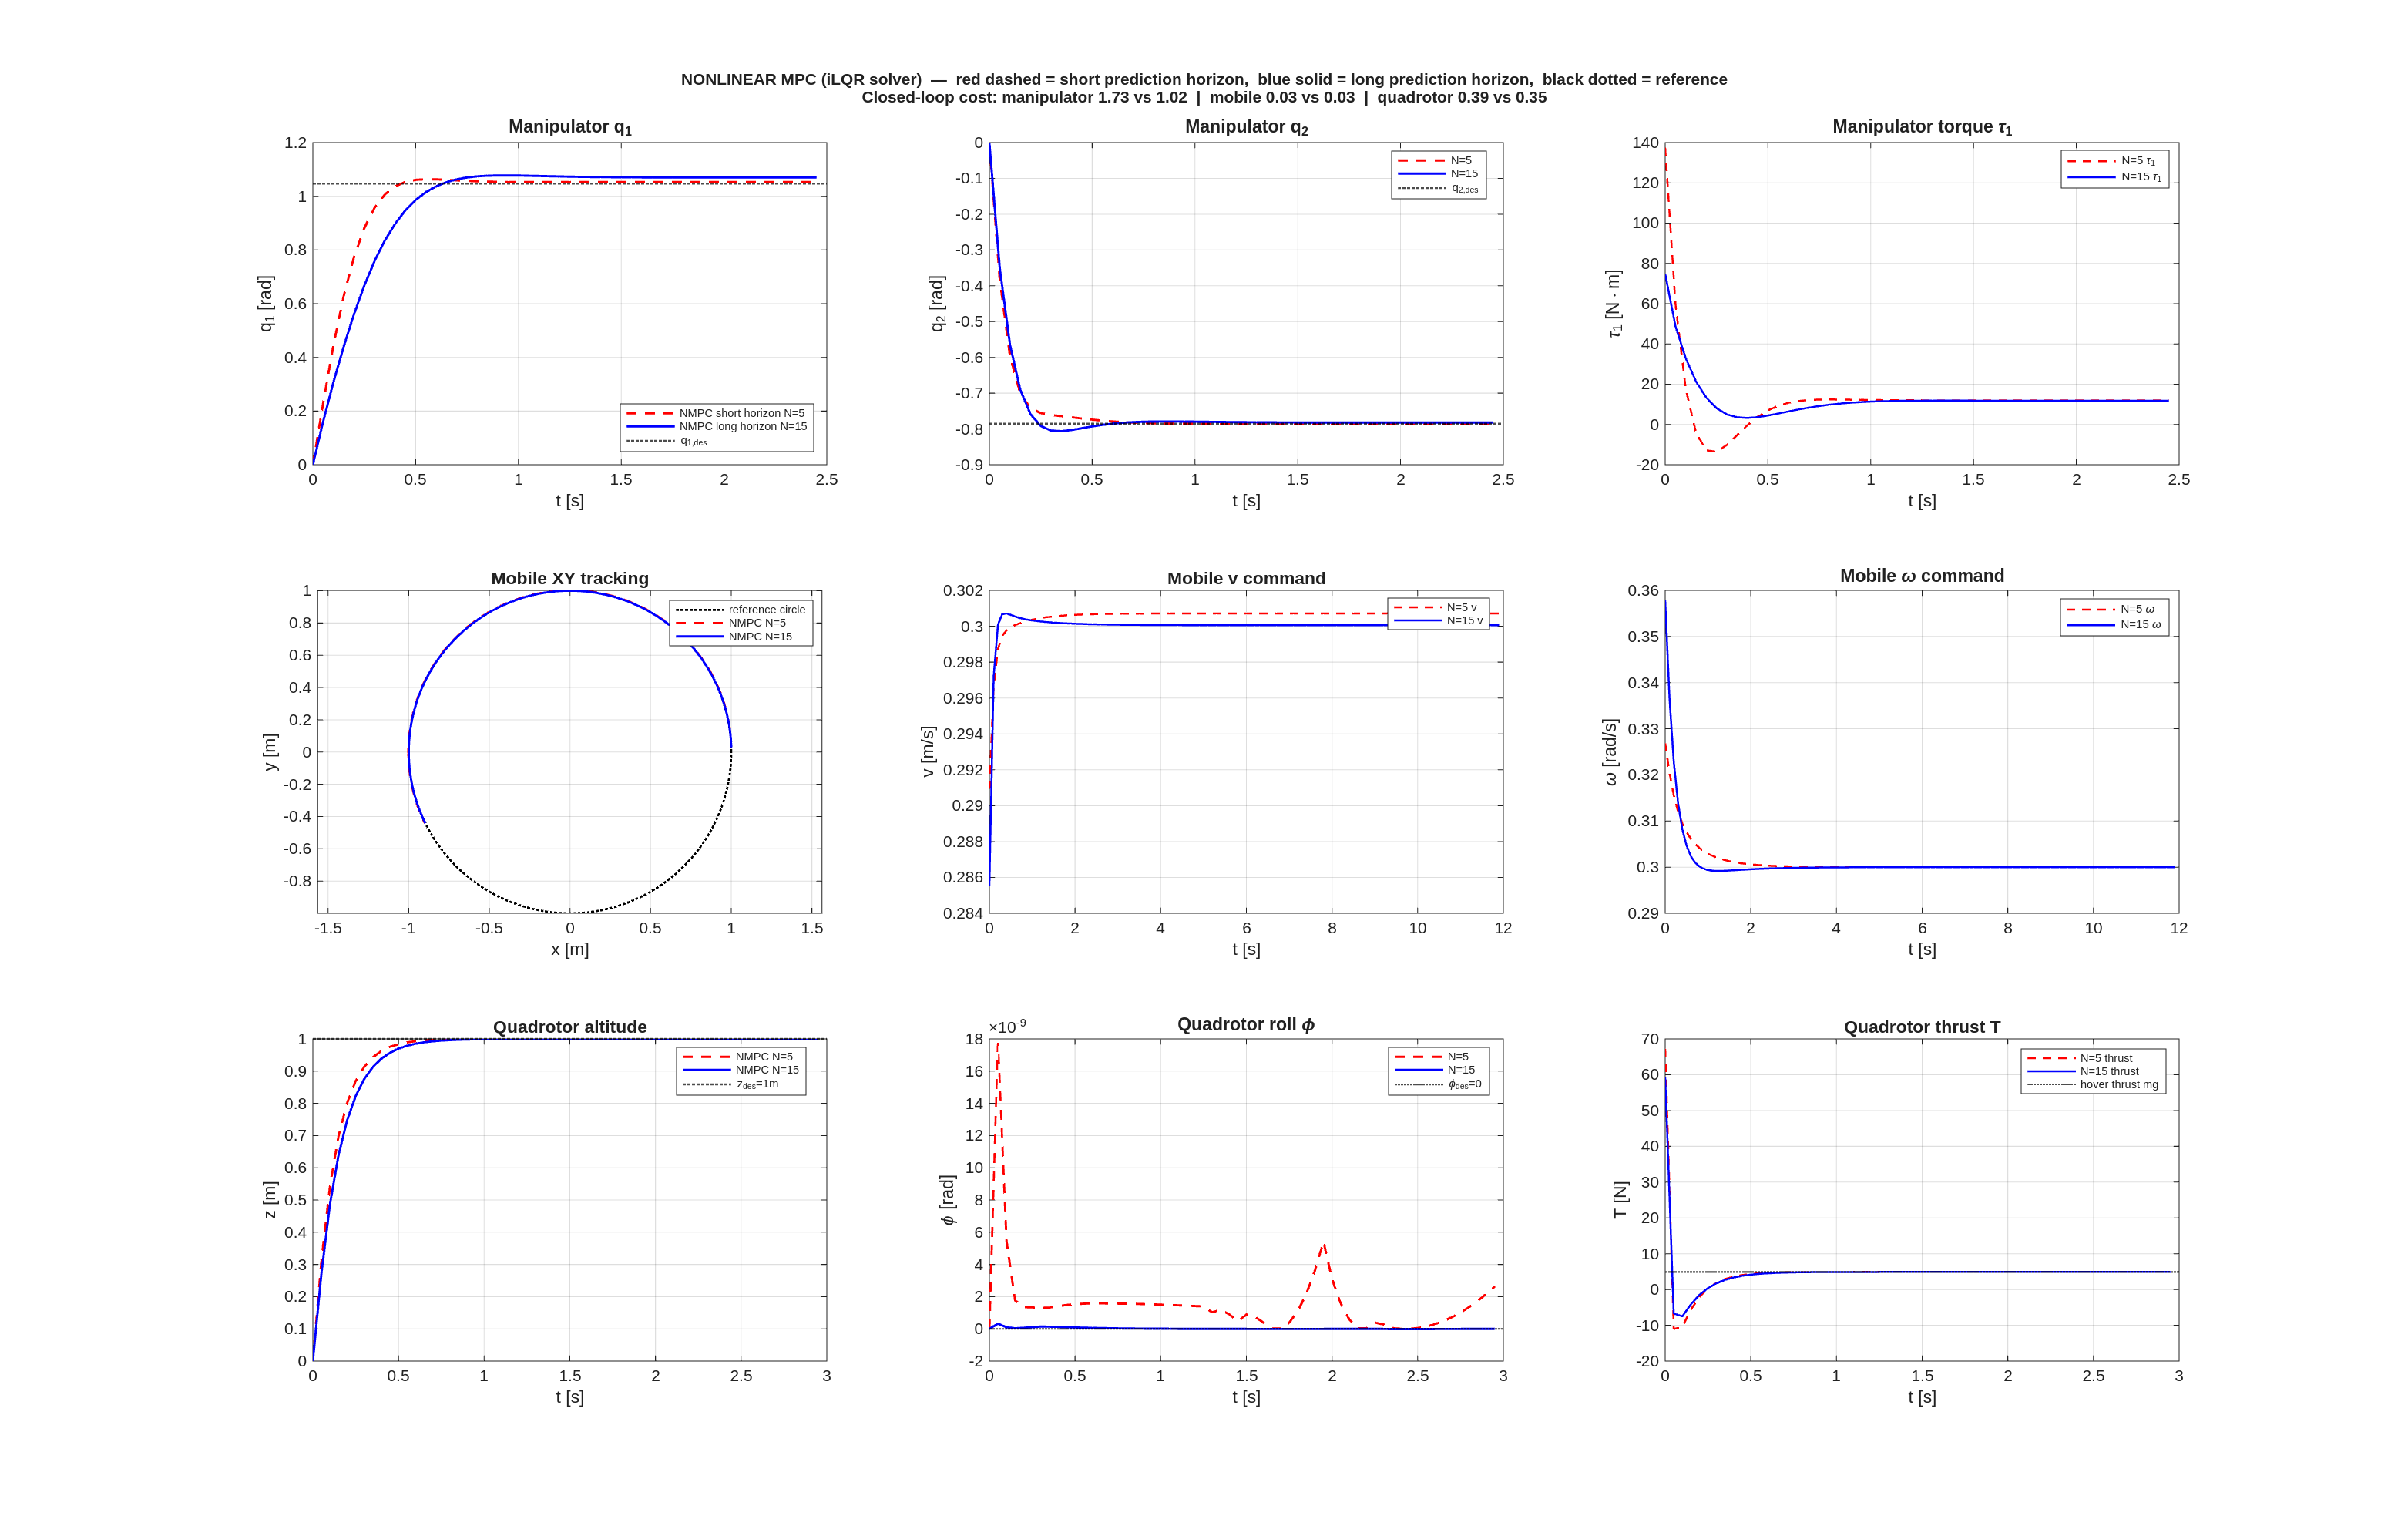
\includegraphics[width=0.85\textwidth]{images/week_08/nmpc_results.png}

Figure 9.1 --- NMPC with short (\textbackslash(N\textbackslash!=\textbackslash!5\textbackslash), red dashed) vs. long (\textbackslash(N\textbackslash!=\textbackslash!15\textbackslash), blue solid) prediction horizon on all three robots. Longer horizon consistently improves or matches the shorter one.

\begin{longtable}[]{@{}lllll@{}}
\toprule\noalign{}
Robot & State dim. & \textbackslash(N\_\{\textbackslash text\{short\}\}\textbackslash) / \textbackslash(J\_\{cl\}\textbackslash) & \textbackslash(N\_\{\textbackslash text\{long\}\}\textbackslash) / \textbackslash(J\_\{cl\}\textbackslash) & Horizon benefit \\
\midrule\noalign{}
\endhead
\bottomrule\noalign{}
\endlastfoot
Manipulator (regulation) & 4 & 5 / 1.730 & 15 / 1.020 & −41.0\% \\
Mobile robot (circle tracking) & 3 & 5 / 0.0313 & 15 / 0.0315 & saturated (both near-perfect) \\
Quadrotor (altitude + attitude) & 6 & 5 / 0.393 & 15 / 0.346 & −12.0\% \\
\end{longtable}

\textbf{Why iLQR works where simplex methods fail:} a 2N-dimensional NLP solved by Nelder-Mead simplex needs \textbackslash(O(10\^{}3)\textbackslash) iterations per sample and still rarely converges. iLQR exploits the \emph{causal structure} of the shooting problem --- one Gauss-Newton step touches every control variable via a single backward sweep --- giving quadratic local convergence in \textbackslash(O(10)\textbackslash) outer iterations.

\textbf{The real-time constraint.} The mobile result is saturated because the unicycle has a 3-state, 2-input model and the circle is easy to track --- horizon 5 is already more than enough. The manipulator and quadrotor both benefit from the longer horizon, as expected for higher-dimensional problems. In deployment, you would profile \texttt{tic/toc} around the solver and shrink the horizon to the shortest value that keeps the stability certificate.

\subsection{Section 10: Unified View --- Every Nonlinear Controller as an Optimization Problem}\label{section-10-unified-view-every-nonlinear-controller-as-an-optimization-problem}}

\subsubsection{10.1 The common template}\label{the-common-template}}

Every controller we have studied fits the pattern:

controller = stability certificate (Lyapunov / CLF / s=0) + free parameters \textbackslash(\textbackslash theta\textbackslash) + performance objective \textbackslash(J(\textbackslash theta)\textbackslash)

Optimization chooses \textbackslash(\textbackslash theta\textbackslash) to minimize \textbackslash(J\textbackslash) subject to the certificate remaining valid.

\subsubsection{10.2 Master summary table}\label{master-summary-table}}

\begin{longtable}[]{@{}lllll@{}}
\toprule\noalign{}
Controller & Decision variables & Cost function & Constraints & Typical solver \\
\midrule\noalign{}
\endhead
\bottomrule\noalign{}
\endlastfoot
Sliding Mode & \textbackslash(\textbackslash lambda,\textbackslash phi,\textbackslash eta\textbackslash) & tracking + effort + chatter & \textbackslash(\textbackslash eta \textgreater{} D\textbackslash), \textbackslash(\textbackslash phi\textgreater0\textbackslash) & fminsearch / BayesOpt / LMI for surface \\
Adaptive (MRAC) & \textbackslash(\textbackslash Gamma,\textbackslash sigma\textbackslash), projection bounds & tracking + effort & \textbackslash(\textbackslash Gamma\textbackslash succ 0,\textbackslash{} \textbackslash sigma\textbackslash geq 0\textbackslash), physical bounds on \textbackslash(\textbackslash hat\textbackslash theta\textbackslash) & fminsearch / BayesOpt \\
Robust (\textbackslash(H\_\textbackslash infty\textbackslash)) & weighting filters \textbackslash(W\_S,W\_T,W\_\{KS\}\textbackslash); or polytopic \textbackslash(K\textbackslash) & \textbackslash(H\_\textbackslash infty\textbackslash) norm of weighted sensitivity & closed-loop stability & hinfsyn / DK-iteration / LMI \\
Backstepping & \textbackslash(k\_1,\textbackslash ldots,k\_n\textbackslash); command-filter BW \textbackslash(\textbackslash omega\_f\textbackslash) & tracking + effort + smoothness & \textbackslash(k\_i\textgreater0\textbackslash), CLF \textbackslash(\textbackslash dot V\_n\textless0\textbackslash) & fminsearch / Bayesian optimization \\
NMPC & \textbackslash(N,Q,R,P,\textbackslash mathcal X\_f,\textbackslash Delta t\textbackslash) & closed-loop integrated cost + solve-time & recursive feasibility, terminal invariance & SQP/IPM + offline LQR for \textbackslash((P,\textbackslash mathcal X\_f)\textbackslash) \\
iLQR / DDP (open-loop) & trajectory \textbackslash(\textbackslash\{u\_k\textbackslash\}\_\{k=0\}\^{}\{N-1\}\textbackslash) & tracking + effort + terminal & dynamics, \textbackslash(u\textbackslash in\textbackslash mathcal U\textbackslash) & iLQR / DDP Newton iterations \\
\end{longtable}

\subsubsection{10.3 Cross-cutting optimization tools}\label{cross-cutting-optimization-tools}}

\paragraph{LMIs \& SDP}\label{lmis-sdp}}

Convex, globally optimal for any Lyapunov-based design that can be posed as an LMI (robust state-feedback, SMC surface, ISS gain).

\paragraph{SOS programming}\label{sos-programming}}

Certifies polynomial Lyapunov functions --- needed for non-quadratic certificates. Backend: SDP.

\paragraph{Bayesian optimization}\label{bayesian-optimization}}

Sample-efficient tuning for black-box controllers on hardware. Minimizes physical trial count when each experiment is expensive.

\paragraph{Reinforcement learning}\label{reinforcement-learning}}

Policy-gradient on a parameterized controller \textbackslash(\textbackslash pi\_\textbackslash theta\textbackslash) --- subsumes all of the above when the reward encodes the cost. Stability not free.

\paragraph{Differentiable simulation}\label{differentiable-simulation}}

Compute \textbackslash(\textbackslash nabla\_\textbackslash theta J\textbackslash) directly through the simulator (autodiff). Gives gradient-based methods the power of BayesOpt at much lower sample cost.

\paragraph{Scenario / stochastic programming}\label{scenario-stochastic-programming}}

Optimizes over a distribution of uncertain parameters rather than a worst case --- average-case robust design.

\subsection{Section 11: MATLAB Lab Activities}\label{section-11-matlab-lab-activities}}

\subsubsection{Setup}\label{setup-3}}

All simulations live in \texttt{week\_08/sims/} and run on base MATLAB (no toolboxes beyond Control System Toolbox required). They use \texttt{fminsearch} for the parameter optimization and explicit Euler or \texttt{ode}-style integration for the dynamics.

\% From MATLAB, cd to the lab directory
cd /home/it-services/auto\_control\_ws/week\_08/sims
\% Run everything (\textasciitilde30 s on a modern laptop)
run\_all
\% Or run a single controller
sim\_smc \% sliding mode
sim\_adaptive \% adaptive / MRAC
sim\_robust \% robust min-max
sim\_backstepping \% backstepping
sim\_nmpc \% nonlinear MPC

\subsubsection{Activity 1 --- SMC Pareto sweep (15 min)}\label{activity-1-smc-pareto-sweep-15-min}}

Inside \texttt{sim\_smc.m}, change the cost weights \textbackslash((w\_e, w\_u, w\_c)\textbackslash) on the chatter term. Re-run and observe:

\begin{itemize}
\tightlist
\item
  Small \textbackslash(w\_c\textbackslash): optimizer picks a \emph{narrow} boundary layer (low \textbackslash(\textbackslash phi\textbackslash)) --- sharp tracking, chattering control
\item
  Large \textbackslash(w\_c\textbackslash): optimizer picks a \emph{wide} boundary layer --- smooth torque, residual tracking error
\end{itemize}

\textbf{Deliverable:} plot the Pareto front of tracking error vs. chatter metric across \textbackslash(w\_c \textbackslash in \textbackslash\{0.001, 0.01, 0.1, 1\textbackslash\}\textbackslash).

\subsubsection{\texorpdfstring{Activity 2 --- Adaptive optimizer tells you when \emph{not} to adapt (10 min)}{Activity 2 --- Adaptive optimizer tells you when not to adapt (10 min)}}\label{activity-2-adaptive-optimizer-tells-you-when-not-to-adapt-10-min}}

Set the payload disturbance to zero in \texttt{sim\_adaptive.m} (make \texttt{p\_true\ =\ p}). Re-run and inspect the optimized \textbackslash(\textbackslash Gamma\textbackslash). Discuss: why does the optimizer drive \textbackslash(\textbackslash Gamma\textbackslash to 0\textbackslash)?

\subsubsection{Activity 3 --- Robust vs. average-case (15 min)}\label{activity-3-robust-vs.-average-case-15-min}}

Modify \texttt{robust\_quad\_cost} to use the \emph{mean} rather than \emph{max} over the uncertainty set. Compare the resulting gains. Under which uncertainty distribution is the average-case design acceptable, and when does the worst-case matter?

\subsubsection{Activity 4 --- NMPC horizon sweep (15 min)}\label{activity-4-nmpc-horizon-sweep-15-min}}

Run \texttt{sim\_nmpc} with the horizon set to \textbackslash(N = \textbackslash\{3,5,7,10,15,25\textbackslash\}\textbackslash) on the quadrotor. Record closed-loop cost \emph{and} per-step solve time (\texttt{tic/toc} around the \texttt{fminsearch} call). Plot both on one graph. Identify the knee of the curve --- this is your deployment horizon.

\textbf{Last run on this machine (R2025b):} total wall time \textasciitilde43~s for all five controllers on all three robots (iLQR-based NMPC dominates the wall-clock). Cost reductions ranged from 2\% (manipulator robust --- already near worst-case optimum) to 88\% (mobile backstepping); NMPC manipulator benefited by 41\% from extending the horizon.

\subsection{Appendix: Week 7 Recall --- Sliding Mode Control (Exam Practice)}\label{appendix-week-7-recall-sliding-mode-control-exam-practice}}

\paragraph{Question 1 --- SMC Controller Design and Stability Proof (25 marks)}\label{question-1-smc-controller-design-and-stability-proof-25-marks}}

Consider a robot manipulator governed by:

\textbackslash{[}
M(q)\textbackslash ddot\{q\} + C(q,\textbackslash dot\{q\})\textbackslash dot\{q\} + G(q) = \textbackslash tau + d(t)
\textbackslash{]}

where \textbackslash(d(t)\textbackslash) represents matched uncertainty with known bound \textbackslash(\textbackslash\textbar d(t)\textbackslash\textbar{} \textbackslash leq D\textbackslash).

\textbf{(a)} Define the tracking error \textbackslash(e = q - q\_d\textbackslash) and the sliding surface:

\textbackslash{[} s = \textbackslash dot\{e\} + \textbackslash Lambda e \textbackslash{]}

where \textbackslash(\textbackslash Lambda = \textbackslash text\{diag\}(\textbackslash lambda\_1, \textbackslash ldots, \textbackslash lambda\_n)\textbackslash) with \textbackslash(\textbackslash lambda\_i \textgreater{} 0\textbackslash). Explain why the system trajectories converge to \textbackslash(e = 0\textbackslash) exponentially once \textbackslash(s = 0\textbackslash).

\paragraph{Model Answer (a)}\label{model-answer-a}}

When \textbackslash(s = 0\textbackslash), \textbackslash(\textbackslash dot e = -\textbackslash Lambda e\textbackslash); with all \textbackslash(\textbackslash lambda\_i\textgreater0\textbackslash), \textbackslash(e(t)=e(0)e\^{}\{-\textbackslash Lambda t\}\textbackslash) converges exponentially with time constants \textbackslash(1/\textbackslash lambda\_i\textbackslash).

\textbf{(b)} Derive the equivalent control \textbackslash(\textbackslash tau\_\{eq\}\textbackslash) by setting \textbackslash(\textbackslash dot\{s\} = 0\textbackslash) (assuming \textbackslash(d = 0\textbackslash)).

\paragraph{Model Answer (b)}\label{model-answer-b}}

\textbackslash{[} \textbackslash boxed\{\textbackslash tau\_\{eq\} = M(q)\textbackslash bigl(\textbackslash ddot\{q\}\_d - \textbackslash Lambda\textbackslash dot\{e\}\textbackslash bigr) + C(q,\textbackslash dot\{q\})\textbackslash dot\{q\} + G(q)\} \textbackslash{]}

\textbf{(c)} With switching term \textbackslash(\textbackslash tau\_\{sw\} = -K\textbackslash,\textbackslash text\{sign\}(s)\textbackslash) and Lyapunov function \textbackslash(V = \textbackslash tfrac\{1\}\{2\}s\^{}\{T\}M(q)s\textbackslash), show \textbackslash(\textbackslash dot V \textbackslash leq -(k\_\{\textbackslash min\}-D)\textbackslash\textbar s\textbackslash\textbar\_1\textbackslash) when \textbackslash(k\_i \textgreater{} D\textbackslash).

\paragraph{Model Answer (c)}\label{model-answer-c}}

Using skew-symmetry of \textbackslash(\textbackslash dot M - 2C\textbackslash): \textbackslash(\textbackslash dot V = s\^{}\{T\}(M\textbackslash dot s + Cs) = s\^{}\{T\}(\textbackslash tau\_\{sw\}+d) = -\textbackslash sum k\_i\textbar s\_i\textbar{} + s\^{}\{T\}d \textbackslash leq -(k\_\{\textbackslash min\}-D)\textbackslash\textbar s\textbackslash\textbar\_1\textbackslash). \textbackslash(\textbackslash square\textbackslash)

\paragraph{Question 2 --- Chattering \& boundary layer (20 marks)}\label{question-2-chattering-boundary-layer-20-marks}}

(a) Explain chattering and why it harms actuators. (b) Derive the steady-state error bound \textbackslash(\textbar e\_\{ss\}\textbar{} \textbackslash leq \textbackslash phi/\textbackslash lambda\textbackslash) for boundary-layer SMC.

\paragraph{Model Answer (condensed)}\label{model-answer-condensed}}

Chattering comes from the discontinuous \textbackslash(\textbackslash text\{sign\}(s)\textbackslash) combined with sampling / unmodelled dynamics. Replacing by \textbackslash(\textbackslash mathrm\{sat\}(s/\textbackslash phi)\textbackslash) yields a high-gain proportional law inside the layer; in steady state \textbackslash(\textbar s\textbar\textbackslash leq \textbackslash phi D/k\textbackslash), and since \textbackslash(s=\textbackslash dot e+\textbackslash lambda e\textbackslash) the tracking-error bound is \textbackslash(\textbar e\_\{ss\}\textbar\textbackslash leq \textbackslash phi/\textbackslash lambda\textbackslash).

\subsection{Section 13: Course Recap \& What\textquotesingle s Next}\label{section-13-course-recap-whats-next}}

\subsubsection{13.1 The nonlinear control theory journey}\label{the-nonlinear-control-theory-journey}}

\paragraph{Weeks 1--3: MPC}\label{weeks-13-mpc}}

Prediction + optimization. Set the stage for NMPC.

\paragraph{Week 4: Adaptive}\label{week-4-adaptive}}

Online parameter learning with Lyapunov certificates.

\paragraph{Week 5: Robust}\label{week-5-robust}}

Fixed controller for worst-case plant.

\paragraph{Week 6: Backstepping}\label{week-6-backstepping}}

Recursive CLF design for strict-feedback systems.

\paragraph{Week 7: SMC}\label{week-7-smc}}

Variable structure, discontinuous robustness.

\paragraph{Week 8 (this): Optimization of all of the above}\label{week-8-this-optimization-of-all-of-the-above}}

Every controller has free parameters; every choice of parameters is an optimization.

\subsubsection{13.2 Unifying themes}\label{unifying-themes}}

\begin{itemize}
\tightlist
\item
  \textbf{Nonlinearity is the defining feature of robots} --- we never linearized at design time in this course.
\item
  \textbf{Lyapunov certificates give the feasible set} of the parameter optimization --- any \textbackslash(\textbackslash theta\textbackslash) that breaks the certificate is excluded.
\item
  \textbf{Optimization is how we pick good controllers, not just good trajectories} --- Section 3.3\textquotesingle s (A) vs (B) distinction.
\item
  \textbf{Compute is a first-class constraint} --- NMPC and adaptive tuning are only useful at real-time sample rates.
\end{itemize}

\subsubsection{13.3 What\textquotesingle s next --- Automation block}\label{whats-next-automation-block}}

Weeks 9--12 shift from control theory to deployment: state machines, ROS 2 integration, perception, and system-level projects. The tuned controllers from this week become the low-level primitives those higher-level systems will invoke.

\textbf{Control for Robots --- M.Sc. Programme}

University of West London • AY 2025--26

Week 8: Nonlinear Control Optimization for Robotic Systems


\pagelayout{wide}
\addpart{ROS\,2 Integration Block}
\pagelayout{wide}

\input{chapters/week_09}
\input{chapters/week_10}
% ----- auto-generated from week_11/Week*.html via pandoc -----
\chapter{ROS\,2 Navigation Control (Week 11)}
\labch{week_11}



Build Costmap, A* Planner, and Path Follower from LiDAR and Odometry Data

Position: Navigation Engineer • Team: Autonomous Navigation\\
Pre-Interview Technical Assessment • Estimated Time: 3 Hours

\section{Overview}

\subsection{Company Brief: AutoNav Solutions}

\textbf{Scenario:} AutoNav Solutions develops autonomous mobile robot platforms for warehouse and logistics environments. Your team has collected 30 seconds of navigation sensor data from a robot operating in a structured environment, including a static map, laser scans, and wheel odometry. As part of this challenge, you will build a complete navigation pipeline from scratch.

\subsection{Provided Bag Data}

\begingroup\footnotesize
\begin{longtable}[]{@{}llll@{}}
\toprule\noalign{}
Topic & Message Type & Rate & Description \\
\midrule\noalign{}
\endhead
\bottomrule\noalign{}
\endlastfoot
\texttt{/map} & nav\_msgs/OccupancyGrid & Latched & Static occupancy grid map of the environment \\
\texttt{/odom} & nav\_msgs/Odometry & 20 Hz & Wheel odometry (position, orientation, velocity) \\
\texttt{/scan} & sensor\_msgs/LaserScan & 5 Hz & 2D laser range finder data \\
\end{longtable}\endgroup

\subsection{Deliverables}

\begin{itemize}
\tightlist
\item
  Costmap generation with static, obstacle, and inflation layers from the provided map and laser data
\item
  A* global path planner operating on the costmap
\item
  A path-following controller (pure pursuit or DWA) as a ROS2 node
\item
  A particle filter (AMCL-style) localisation node fusing odometry and laser scan data
\item
  A quantitative comparison of path quality, tracking error, and localisation accuracy
\end{itemize}

\subsection{Evaluation Criteria}

\begin{itemize}
\tightlist
\item
  \textbf{Navigation Architecture:} Proper separation of planning, control, and localisation components
\item
  \textbf{Algorithm Correctness:} Valid A* implementation, correct costmap inflation, stable particle filter
\item
  \textbf{Integration:} Components working together through ROS2 topics and action servers
\item
  \textbf{Communication:} Ability to explain Nav2 architecture and compare DWA to MPC during the follow-up interview
\end{itemize}

\subsection{Skills You Will Demonstrate}

By the end of this session, you will be able to:

\begin{itemize}
\tightlist
\item
  Describe the ROS2 Nav2 architecture and explain how global planner, local controller, costmap, AMCL, and behavior tree components interact through ROS2 topics and action servers.
\item
  Configure costmap layers (static, obstacle, inflation) and explain how the inflation cost function creates soft constraints analogous to MPC barrier functions.
\item
  Analyse the Dynamic Window Approach (DWA) as an optimization-based local controller and compare its cost function to the MPC formulation studied in Week 3.
\item
  Explain how AMCL implements a particle filter for robot localization, connecting it to the controller-estimator pairing required by the NMPC / iLQR framework of Week 8.
\item
  Design and interpret behavior trees for mission-level navigation control, comparing them with finite state machines.
\item
  Integrate PID, LQR, and MPC controllers with the Nav2 navigation stack as local controller plugins.
\item
  Compare the suitability of different control approaches (PID, MPC, SMC, Backstepping, Robust, Adaptive) for various mobile robot navigation scenarios.
\item
  Configure, launch, and tune Nav2 for TurtleBot3 simulation including AMCL localization, DWA local planning, and waypoint navigation.
\end{itemize}

\subsection{Recommended Approach (3-Hour Session)}

0:00 -- 0:20

\subsubsection{Week 10 Exam Recall \& Introduction}

Review quadrotor control exam questions. Introduce mobile robot navigation as the next control application domain.

0:20 -- 0:50

\subsubsection{Nav2 Architecture Overview}

Global planner, local controller, costmaps, AMCL, behavior trees, recovery behaviors. Key ROS2 topics and message types.

0:50 -- 1:20

\subsubsection{DWA --- The Local Controller as Optimization}

Deep dive into the Dynamic Window Approach. Connection to MPC. Simplified DWA implementation in ROS2.

1:20 -- 1:35

\subsubsection{Break}

15-minute break.

1:35 -- 1:55

\subsubsection{AMCL --- State Estimation for Control}

Particle filter localization. Connection to Week 8\textquotesingle s controller-estimator pairing for NMPC. ROS2 AMCL configuration.

1:55 -- 2:10

\subsubsection{Costmaps as Constraints \& Part 5: Behavior Trees}

Costmap inflation as soft constraints. Behavior tree navigation orchestration.

2:10 -- 2:25

\subsubsection{Applying Control Theory to Navigation}

Mapping all 8 control methods from the course to mobile robot navigation scenarios.

2:25 -- 3:00

\subsubsection{Hands-On Activities \& Lab Exercises}

Configure Nav2 for TurtleBot3. Tune DWA. Compare DWA vs MPC. Waypoint navigation with recovery.

\section{The ROS2 Navigation Stack (Nav2)}

Nav2 is the standard ROS2 navigation framework for autonomous mobile robots. It provides a complete, modular pipeline: from a goal pose, through path planning and obstacle avoidance, to velocity commands sent to the robot\textquotesingle s motors. Every component is a ROS2 lifecycle node that can be configured, replaced, or extended via plugins.

\subsection{Nav2 Core Components}

\subsubsection{Global Planner}

Computes a collision-free path from the robot\textquotesingle s current position to the goal on the global costmap. Plugins include \textbf{NavFn} (Dijkstra/A*), \textbf{SmacPlanner} (State Lattice, Hybrid-A*), and \textbf{ThetaStar}. Operates on the full map at \textasciitilde1 Hz.

\subsubsection{Local Controller}

Follows the global path while avoiding local obstacles. Runs at 10--20 Hz on the local costmap. Plugins: \textbf{DWA} (Dynamic Window Approach), \textbf{MPPI} (Model Predictive Path Integral), \textbf{Regulated Pure Pursuit}, \textbf{Rotation Shim}.

\subsubsection{Costmap 2D}

Layered 2D cost grid. \textbf{Static layer} from the SLAM map, \textbf{obstacle layer} from live sensor data (LiDAR, depth cameras), \textbf{inflation layer} providing safety buffers with exponential cost decay around obstacles.

\subsubsection{AMCL Localization}

Adaptive Monte Carlo Localization --- a particle filter that estimates the robot\textquotesingle s pose on the map using laser scan data and odometry. Publishes the \texttt{map\ →\ odom} transform.

\subsubsection{Behavior Tree Navigator}

Orchestrates the entire navigation pipeline using behavior trees (BehaviorTree.CPP). Handles sequencing of planning, control, and recovery. More flexible and maintainable than finite state machines.

\subsubsection{Recovery Behaviors}

Activated when the robot gets stuck. \textbf{Spin:} rotate in place to clear local costmap. \textbf{Backup:} drive backwards. \textbf{Wait:} pause and hope dynamic obstacles move. \textbf{ClearCostmap:} reset costmap layers.

\subsection{Nav2 Architecture Diagram}

\subsection{Key Nav2 ROS2 Topics}

\begingroup\footnotesize
\begin{longtable}[]{@{}llll@{}}
\toprule\noalign{}
Topic & Message Type & Publisher & Purpose \\
\midrule\noalign{}
\endhead
\bottomrule\noalign{}
\endlastfoot
\texttt{/map} & \texttt{nav\_msgs/OccupancyGrid} & Map Server & Static occupancy grid from SLAM. Values: 0 = free, 100 = occupied, -1 = unknown. \\
\texttt{/scan} & \texttt{sensor\_msgs/LaserScan} & LiDAR driver & 2D laser range data. Used by AMCL for localization and obstacle layer for costmap. \\
\texttt{/odom} & \texttt{nav\_msgs/Odometry} & Wheel encoders & Robot odometry (pose + twist). Frame: odom → base\_link. \\
\texttt{/cmd\_vel} & \texttt{geometry\_msgs/Twist} & Local Controller & Velocity command: \texttt{linear.x} (m/s), \texttt{angular.z} (rad/s) for differential drive. \\
\texttt{/global\_costmap/costmap} & \texttt{nav\_msgs/OccupancyGrid} & Costmap 2D & Full-map costmap used by global planner. Updated at \textasciitilde1 Hz. \\
\texttt{/local\_costmap/costmap} & \texttt{nav\_msgs/OccupancyGrid} & Costmap 2D & Rolling-window costmap centred on robot. Used by local controller at 5--20 Hz. \\
\texttt{/plan} & \texttt{nav\_msgs/Path} & Global Planner & Sequence of poses from current position to goal. \\
\texttt{/tf}, \texttt{/tf\_static} & \texttt{tf2\_msgs/TFMessage} & Various & Transform tree: map → odom → base\_link → sensors. Critical for all Nav2 components. \\
\end{longtable}\endgroup

\textbf{Control Theory Connection:} The Nav2 architecture implements a hierarchical control structure analogous to the cascaded quadrotor controller from Week 10. The behavior tree is the mission-level controller, the global planner is the trajectory generator, and the local controller is the real-time feedback loop --- each operating at progressively faster rates.

\section{DWA: The Local Controller as Optimization}

The Dynamic Window Approach (DWA) is one of the most widely-used local planners in mobile robotics. From a control theory perspective, \textbf{DWA is essentially a simplified Model Predictive Controller with a one-step prediction horizon}. Understanding this connection bridges the gap between classical control optimization (Week 3) and practical robot navigation.

\subsection{DWA Velocity Space}

A differential-drive robot is controlled by two inputs: linear velocity \(v\) and angular velocity \(\omega\). DWA operates in this 2D velocity space:

\textbf{Velocity Space:} \((v, \omega)\) where \(v \in [v_{\min}, v_{\max}]\), \(\omega \in [\omega_{\min}, \omega_{\max}]\)

\subsection{Dynamic Window Constraint}

Not all velocities in the admissible range are physically reachable from the current state within one control interval \(\Delta t\). The \textbf{dynamic window} restricts the search to reachable velocities given acceleration limits:

\[
        V_d = \{ (v, \omega) \mid v \in [v_c - \dot{v}_{\max}\Delta t,\; v_c + \dot{v}_{\max}\Delta t], \;
        \omega \in [\omega_c - \dot{\omega}_{\max}\Delta t,\; \omega_c + \dot{\omega}_{\max}\Delta t] \}
        \]

where \((v_c, \omega_c)\) is the current velocity and \((\dot{v}_{\max}, \dot{\omega}_{\max})\) are the maximum accelerations.

The \textbf{admissible velocities} are further constrained to those that allow the robot to stop before hitting an obstacle:

\[
        V_a = \{ (v, \omega) \mid v \leq \sqrt{2 \cdot \text{dist}(v,\omega) \cdot \dot{v}_{\max}},\;
        \omega \leq \sqrt{2 \cdot \text{dist}(v,\omega) \cdot \dot{\omega}_{\max}} \}
        \]

\subsection{DWA Objective Function}

DWA selects the velocity pair \((v^*, \omega^*)\) that maximises a weighted objective:

\[ G(v, \omega) = \alpha \cdot \text{heading}(v,\omega) + \beta \cdot \text{clearance}(v,\omega) + \gamma \cdot \text{velocity}(v,\omega) \]

where:

\begin{itemize}
\tightlist
\item
  \textbf{heading(\(v, \omega\)):} Measures alignment of the predicted trajectory\textquotesingle s endpoint with the goal direction. Defined as \(180^\circ - |\theta_{\text{goal}} - \theta_{\text{endpoint}}|\), normalised to {[}0, 1{]}. Encourages the robot to face the goal.
\item
  \textbf{clearance(\(v, \omega\)):} Minimum distance from the predicted trajectory to the nearest obstacle. Larger clearance = safer trajectory. Returns \(-\infty\) for collision trajectories (hard constraint).
\item
  \textbf{velocity(\(v, \omega\)):} Forward speed \(v\) of the candidate, normalised to {[}0, 1{]}. Encourages faster progress toward the goal rather than overly cautious creeping.
\end{itemize}

\subsection{Connection to MPC (Week 3)}

\textbf{Key Insight:} DWA can be viewed as MPC with horizon \(N = 1\), state = robot pose, control = \((v, \omega)\), cost = negative of heading + clearance + velocity, and constraints = dynamic window + collision-free. The modern Nav2 \textbf{MPPI} (Model Predictive Path Integral) controller IS full MPC with \(N \gg 1\).

\textbf{DWA Cost (1-step optimisation):}

\[ \min_{v, \omega} -\bigl[\alpha \cdot h(v,\omega) + \beta \cdot c(v,\omega) + \gamma \cdot v\bigr] \quad \text{s.t.} \quad (v,\omega) \in V_d \cap V_a \]

\hfill\break

\textbf{MPC Cost (N-step optimisation, Week 3):}

\[ \min_{\mathbf{u}_{0:N-1}} \sum_{k=0}^{N-1} \bigl[\mathbf{x}_k^T \mathbf{Q} \mathbf{x}_k + \mathbf{u}_k^T \mathbf{R} \mathbf{u}_k\bigr] + \mathbf{x}_N^T \mathbf{P} \mathbf{x}_N \quad \text{s.t. model, constraints} \]

\begingroup\footnotesize
\begin{longtable}[]{@{}lll@{}}
\toprule\noalign{}
Aspect & DWA & MPC \\
\midrule\noalign{}
\endhead
\bottomrule\noalign{}
\endlastfoot
Prediction Horizon & \(N = 1\) (or short trajectory) & \(N \gg 1\) (10--50 steps) \\
Decision Variables & \((v, \omega)\) --- 2 scalars & \(\mathbf{u}_{0:N-1}\) --- \(2N\) variables \\
Optimisation Method & Grid search over sampled velocities & QP solver or sampling (MPPI) \\
Constraint Handling & Dynamic window + collision check & Explicit inequality constraints \\
Computational Cost & Low (\textasciitilde1 ms) & Higher (\textasciitilde5--50 ms) \\
Anticipation & Myopic (reacts to immediate surroundings) & Looks ahead (anticipates obstacles, turns) \\
\end{longtable}\endgroup

\subsection{ROS2 Implementation --- Simplified DWA Local Planner Node}

\begin{verbatim}
#!/usr/bin/env python3
"""Simplified DWA local planner node for ROS2.
Subscribes to /odom and /plan, publishes /cmd_vel.
Demonstrates DWA as optimization-based control."""

import rclpy
from rclpy.node import Node
import numpy as np
import math
from nav_msgs.msg import Odometry, Path
from geometry_msgs.msg import Twist
from sensor_msgs.msg import LaserScan

class DWAControllerNode(Node):
    def __init__(self):
        super().__init__('dwa_controller')
        # DWA parameters
        self.max_v = 0.5;  self.min_v = 0.0
        self.max_w = 1.0;  self.max_accel = 0.5;  self.max_w_accel = 1.0
        self.v_res = 0.05;  self.w_res = 0.1
        self.dt = 0.1;  self.predict_time = 2.0
        self.alpha = 1.0;  self.beta = 0.8;  self.gamma = 0.5  # heading, clearance, velocity
        self.robot_radius = 0.18
        # State
        self.x, self.y, self.th = 0.0, 0.0, 0.0
        self.cur_v, self.cur_w = 0.0, 0.0
        self.goal = None;  self.obstacles = []
        # ROS2 interfaces
        self.create_subscription(Odometry, '/odom', self.odom_cb, 10)
        self.create_subscription(Path, '/plan', self.path_cb, 10)
        self.create_subscription(LaserScan, '/scan', self.scan_cb, 10)
        self.cmd_pub = self.create_publisher(Twist, '/cmd_vel', 10)
        self.timer = self.create_timer(0.1, self.control_loop)  # 10 Hz
        self.get_logger().info('DWA Controller started')

    def odom_cb(self, msg):
        self.x = msg.pose.pose.position.x
        self.y = msg.pose.pose.position.y
        q = msg.pose.pose.orientation
        self.th = 2.0 * math.atan2(q.z, q.w)
        self.cur_v = msg.twist.twist.linear.x
        self.cur_w = msg.twist.twist.angular.z

    def path_cb(self, msg):
        if msg.poses:
            p = msg.poses[-1].pose.position  # Use final pose as goal
            self.goal = (p.x, p.y)

    def scan_cb(self, msg):
        obs = []
        for i, r in enumerate(msg.ranges):
            if msg.range_min < r < msg.range_max:
                angle = msg.angle_min + i * msg.angle_increment
                ox = self.x + r * math.cos(self.th + angle)
                oy = self.y + r * math.sin(self.th + angle)
                obs.append((ox, oy))
        self.obstacles = obs

    def predict_trajectory(self, v, w):
        """Forward-simulate trajectory for predict_time seconds."""
        x, y, th = self.x, self.y, self.th
        traj = [(x, y)]
        for _ in range(int(self.predict_time / self.dt)):
            x += v * math.cos(th) * self.dt
            y += v * math.sin(th) * self.dt
            th += w * self.dt
            traj.append((x, y))
        return traj, th

    def score_trajectory(self, traj, final_th):
        """Score: alpha*heading + beta*clearance + gamma*velocity."""
        if not self.goal:
            return -float('inf')
        ex, ey = traj[-1]
        # Heading: alignment with goal
        goal_angle = math.atan2(self.goal[1] - ey, self.goal[0] - ex)
        heading = math.pi - abs(goal_angle - final_th)
        heading = heading / math.pi  # normalise to [0, 1]
        # Clearance: min distance to obstacles
        clearance = float('inf')
        for (px, py) in traj:
            for (ox, oy) in self.obstacles:
                d = math.hypot(px - ox, py - oy)
                clearance = min(clearance, d)
        if clearance < self.robot_radius:
            return -float('inf')  # Collision!
        clearance = min(clearance, 3.0) / 3.0  # normalise
        # Velocity: prefer faster
        velocity = abs(traj[-1][0] - traj[0][0]) + abs(traj[-1][1] - traj[0][1])
        velocity = min(velocity, 1.0)
        return self.alpha * heading + self.beta * clearance + self.gamma * velocity

    def control_loop(self):
        if self.goal is None:
            return
        if math.hypot(self.x - self.goal[0], self.y - self.goal[1]) < 0.2:
            self.cmd_pub.publish(Twist());  return  # Goal reached
        # Dynamic window
        v_lo = max(self.min_v, self.cur_v - self.max_accel * self.dt)
        v_hi = min(self.max_v, self.cur_v + self.max_accel * self.dt)
        w_lo = max(-self.max_w, self.cur_w - self.max_w_accel * self.dt)
        w_hi = min(self.max_w, self.cur_w + self.max_w_accel * self.dt)
        # Sample and score
        best_v, best_w, best_score = 0.0, 0.0, -float('inf')
        v = v_lo
        while v <= v_hi:
            w = w_lo
            while w <= w_hi:
                traj, fth = self.predict_trajectory(v, w)
                s = self.score_trajectory(traj, fth)
                if s > best_score:
                    best_score, best_v, best_w = s, v, w
                w += self.w_res
            v += self.v_res
        # Publish best command
        cmd = Twist()
        cmd.linear.x = best_v;  cmd.angular.z = best_w
        self.cmd_pub.publish(cmd)

def main(args=None):
    rclpy.init(args=args)
    rclpy.spin(DWAControllerNode())
    rclpy.shutdown()

if __name__ == '__main__':
    main()
\end{verbatim}

\textbf{Tuning Guide:} The weights \(\alpha, \beta, \gamma\) dramatically affect robot behavior.
High \(\alpha\) = aggressive goal-seeking (may clip obstacles).
High \(\beta\) = overly cautious (slow progress).
High \(\gamma\) = fast but may overshoot.
Start with \(\alpha = 1.0, \beta = 1.0, \gamma = 0.5\) and adjust.

\section{AMCL: State Estimation for Control}

\subsection{Connection to Nonlinear Optimization (Week 8)}

Week 8 developed \textbf{nonlinear control optimization for robotic systems}: iLQR/NMPC for trajectory optimization, and per-controller optimization of SMC / adaptive / robust / backstepping gains. Every controller in that framework assumes access to the state \(x\) --- but in a real robot the state must be \emph{estimated} from sensors. Controller-plus-estimator is the universal structure:

\subsubsection{Week 8 NMPC / iLQR}

\begin{itemize}
\tightlist
\item
  \textbf{Controller:} NMPC via iLQR (optimal nonlinear control, local feedback policy)
\item
  \textbf{Estimator:} matched to the dynamics --- EKF/UKF if the posterior is unimodal, particle filter if multimodal
\item
  \textbf{State:} full nonlinear state \(x\in\mathbb R^n\)
\item
  \textbf{Sensors:} any; noise model enters the estimator design, not the controller
\end{itemize}

\subsubsection{Nav2 Navigation}

\begin{itemize}
\tightlist
\item
  \textbf{Controller:} DWA / MPPI / Pure Pursuit (all are finite-horizon optimizers --- DWA is a one-step discrete search; MPPI is sampling-based NMPC)
\item
  \textbf{Estimator:} AMCL (particle filter)
\item
  \textbf{State:} Robot pose \((x, y, \theta)\) on a map
\item
  \textbf{Sensors:} Laser scans + odometry (non-Gaussian, multimodal posterior)
\end{itemize}

\textbf{Why not a Kalman Filter?} The Kalman filter assumes Gaussian distributions and linear (or locally linear) models. In mobile robot localization, the probability distribution over poses can be \textbf{multimodal} (the robot could be in several places on a symmetric map). Particle filters handle arbitrary distributions, making AMCL more suitable for global localization.

\subsection{AMCL Algorithm}

AMCL represents the belief over the robot\textquotesingle s pose as a set of weighted particles:

\textbf{Particle Set:} \(\mathcal{X} = \{(x_i, y_i, \theta_i, w_i)\}_{i=1}^{N}\)

where each particle \(i\) has pose \((x_i, y_i, \theta_i)\) and weight \(w_i\) with \(\sum_{i=1}^{N} w_i = 1\).

The AMCL algorithm cycles through four steps:

\begin{enumerate}
\tightlist
\item
  \textbf{Motion Update (Prediction):} Propagate each particle using the odometry motion model with added noise:
  \[ x_i' = x_i + \delta_{\text{trans}} \cos(\theta_i + \delta_{\text{rot1}}) + \epsilon_x \]
  \[ y_i' = y_i + \delta_{\text{trans}} \sin(\theta_i + \delta_{\text{rot1}}) + \epsilon_y \]
  \[ \theta_i' = \theta_i + \delta_{\text{rot1}} + \delta_{\text{rot2}} + \epsilon_\theta \]
  where \(\epsilon\) terms are sampled from noise distributions parameterised by odometry noise coefficients \((\alpha_1, \alpha_2, \alpha_3, \alpha_4)\).
\item
  \textbf{Measurement Update (Correction):} Weight each particle by the likelihood of the observed laser scan given that particle\textquotesingle s pose. Using the likelihood field model:
  \[ w_i = \prod_{j \in \text{beams}} \bigl[ z_{\text{hit}} \cdot \mathcal{N}(d_j; 0, \sigma^2) + z_{\text{random}} \cdot \tfrac{1}{z_{\max}} \bigr] \]
  where \(d_j\) is the distance from the beam endpoint to the nearest obstacle in the map.
\item
  \textbf{Normalisation:} \(w_i \leftarrow w_i / \sum_{k=1}^{N} w_k\)
\item
  \textbf{Resampling:} When the effective particle count \(N_{\text{eff}} = 1/\sum w_i^2\) drops below a threshold, perform low-variance resampling: draw a new particle set where particles with higher weights are more likely to be selected.
\end{enumerate}

\subsection{AMCL Cycle Diagram}

\subsection{ROS2 AMCL Configuration}

\begin{verbatim}
# Launch AMCL for TurtleBot3 localization
ros2 launch nav2_bringup localization_launch.py \
    map:=/path/to/map.yaml \
    params_file:=/path/to/nav2_params.yaml
\end{verbatim}

Key AMCL parameters in \texttt{nav2\_params.yaml}:

\begin{verbatim}
AMCL Parameters (nav2_params.yaml)
\end{verbatim}

amcl:
ros\_\_parameters:
min\_particles: 500 \# Minimum particle count
max\_particles: 2000 \# Maximum particle count (adaptive)
update\_min\_d: 0.25 \# Min translation (m) before update
update\_min\_a: 0.2 \# Min rotation (rad) before update
laser\_model\_type: "likelihood\_field"
laser\_max\_range: 12.0
laser\_min\_range: 0.1
odom\_model\_type: "diff-corrected"
\# Odometry noise parameters (alpha1-alpha4)
robot\_model\_type: "differential"
alpha1: 0.2 \# Rotation noise from rotation
alpha2: 0.2 \# Rotation noise from translation
alpha3: 0.2 \# Translation noise from translation
alpha4: 0.2 \# Translation noise from rotation
\# Likelihood field parameters
z\_hit: 0.95
z\_rand: 0.05
sigma\_hit: 0.2
\# Recovery
recovery\_alpha\_slow: 0.001 \# Slow average weight decay
recovery\_alpha\_fast: 0.1 \# Fast average weight decay

\section{Costmap: Constraints for Control}

In control theory, constraints define the safe operating region. In Nav2, \textbf{costmaps} serve exactly this purpose: they encode where the robot can and cannot go, with graduated costs creating soft boundaries.

\subsection{Costmaps as Control Constraints}

\subsubsection{Global Costmap ↔ Terminal Constraint}

The global costmap constrains the global planner, analogous to the \textbf{terminal constraint} in MPC that ensures the planned trajectory ends in a safe set. It covers the entire known map and updates slowly (\textasciitilde1 Hz).

\subsubsection{Local Costmap ↔ Stage Constraints}

The local costmap constrains the DWA/MPPI local controller, analogous to \textbf{stage constraints} in MPC \((\mathbf{x}_k \in \mathcal{X}, \mathbf{u}_k \in \mathcal{U})\) that enforce safety at each time step. Rolling window, updated at 5--20 Hz.

\subsubsection{Inflation Layer ↔ Soft Constraints}

The inflation layer creates graduated costs around obstacles, analogous to \textbf{barrier functions} or \textbf{soft constraints} with penalty terms. The robot is not forbidden from approaching obstacles but incurs increasing cost.

\subsection{Costmap Layers}

\begin{enumerate}
\tightlist
\item
  \textbf{Static Layer:} Loaded from the SLAM-generated map. Contains walls, permanent furniture, and other fixed obstacles. Values: 0 (free), 100 (occupied), -1 (unknown).
\item
  \textbf{Obstacle Layer:} Populated from live sensor data (LiDAR, depth cameras). Detects dynamic obstacles not in the static map --- people, other robots, moved furniture. Marks cells as lethal (254) based on sensor readings.
\item
  \textbf{Inflation Layer:} Expands obstacles by the robot\textquotesingle s inscribed radius and adds exponentially-decaying cost beyond that. This is the critical safety layer.
\end{enumerate}

\subsection{Inflation Cost Function}

\[
        c(d) = \begin{cases}
            254 \;\text{(LETHAL)} & \text{if } d < r_{\text{inscribed}} \\[6pt]
            A \cdot e^{-\beta \,(d - r_{\text{inscribed}})} & \text{if } r_{\text{inscribed}} \leq d \leq r_{\text{inflation}} \\[6pt]
            0 \;\text{(FREE)} & \text{if } d > r_{\text{inflation}}
        \end{cases}
        \]

where:

\begin{itemize}
\tightlist
\item
  \(d\) = distance from the cell to the nearest obstacle
\item
  \(r_{\text{inscribed}}\) = inscribed radius of the robot footprint (if the robot centre is closer than this, collision is guaranteed)
\item
  \(r_{\text{inflation}}\) = outer inflation radius (beyond this, cost is zero)
\item
  \(A = 253\) (INSCRIBED cost value, just below LETHAL)
\item
  \(\beta\) = cost scaling factor controlling how quickly cost decays with distance
\end{itemize}

\subsection{Nav2 Costmap Configuration}

\begin{verbatim}
Costmap YAML Configuration (nav2_params.yaml)
\end{verbatim}

global\_costmap:
global\_costmap:
ros\_\_parameters:
update\_frequency: 1.0
publish\_frequency: 1.0
global\_frame: map
robot\_base\_frame: base\_link
resolution: 0.05 \# 5cm per cell
track\_unknown\_space: true
plugins: {[}"static\_layer", "obstacle\_layer", "inflation\_layer"{]}
static\_layer:
plugin: "nav2\_costmap\_2d::StaticLayer"
map\_subscribe\_transitioned\_to\_active: true
obstacle\_layer:
plugin: "nav2\_costmap\_2d::ObstacleLayer"
enabled: true
observation\_sources: scan
scan:
topic: /scan
max\_obstacle\_height: 2.0
clearing: true
marking: true
raytrace\_max\_range: 3.0
obstacle\_max\_range: 2.5
inflation\_layer:
plugin: "nav2\_costmap\_2d::InflationLayer"
cost\_scaling\_factor: 5.0 \# beta in the formula
inflation\_radius: 0.55 \# r\_inflation in meters
local\_costmap:
local\_costmap:
ros\_\_parameters:
update\_frequency: 5.0
publish\_frequency: 2.0
global\_frame: odom
robot\_base\_frame: base\_link
rolling\_window: true
width: 3 \# 3m x 3m window
height: 3
resolution: 0.05
plugins: {[}"obstacle\_layer", "inflation\_layer"{]}
obstacle\_layer:
plugin: "nav2\_costmap\_2d::ObstacleLayer"
enabled: true
observation\_sources: scan
scan:
topic: /scan
max\_obstacle\_height: 2.0
clearing: true
marking: true
inflation\_layer:
plugin: "nav2\_costmap\_2d::InflationLayer"
cost\_scaling\_factor: 5.0
inflation\_radius: 0.55

\section{Behavior Trees for Mission Control}

\subsection{Why Behavior Trees?}

Behavior Trees (BTs) are an alternative to Finite State Machines (FSMs) for orchestrating complex robot behaviors. Nav2 uses the \textbf{BehaviorTree.CPP} library.

\begingroup\footnotesize
\begin{longtable}[]{@{}lll@{}}
\toprule\noalign{}
Aspect & Finite State Machine & Behavior Tree \\
\midrule\noalign{}
\endhead
\bottomrule\noalign{}
\endlastfoot
Structure & States + transitions (graph) & Tree of nodes (hierarchical) \\
Scalability & Exponential transitions as states grow & Modular subtrees, easy to extend \\
Reactivity & Must explicitly handle every transition & Built-in: tick propagation handles preemption \\
Reusability & Low (states are context-dependent) & High (subtrees are self-contained) \\
Debugging & Hard with many states & Visual tools (Groot) show live tree state \\
\end{longtable}\endgroup

\subsection{BT Node Types}

\begin{itemize}
\tightlist
\item
  \textbf{Sequence (→):} Execute children left-to-right. Returns SUCCESS if all succeed, FAILURE if any fails, RUNNING if a child is still executing.
\item
  \textbf{Fallback (?):} Try children left-to-right until one succeeds. Returns SUCCESS on first success, FAILURE if all fail. Used for recovery.
\item
  \textbf{Action:} Leaf node that performs work (e.g., ComputePath, FollowPath, Spin, Backup).
\item
  \textbf{Condition:} Leaf node that checks state (e.g., IsGoalReached, IsBatteryLow). Returns SUCCESS or FAILURE.
\item
  \textbf{Decorator:} Modifies a child\textquotesingle s behavior (e.g., Inverter, Retry, Timeout).
\end{itemize}

\subsection{Navigation Behavior Tree Diagram}

\subsection{Nav2 BT XML Configuration}

\begin{verbatim}
Default Nav2 Behavior Tree XML (navigate_to_pose_w_replanning.xml)
\end{verbatim}

\textless root main\_tree\_to\_execute="MainTree"\textgreater{}
\textless BehaviorTree ID="MainTree"\textgreater{}
\textless RecoveryNode number\_of\_retries="6" name="NavigateRecovery"\textgreater{}
\textless PipelineSequence name="NavigateWithReplanning"\textgreater{}
\textless RateController hz="1.0"\textgreater{}
\textless ComputePathToPose goal="\{goal\}" path="\{path\}"
planner\_id="GridBased"/\textgreater{}
\textless/RateController\textgreater{}
\textless FollowPath path="\{path\}" controller\_id="FollowPath"/\textgreater{}
\textless/PipelineSequence\textgreater{}
\textless SequenceStar name="RecoveryActions"\textgreater{}
\textless ClearEntireCostmap name="ClearLocalCostmap"
service\_name="/local\_costmap/clear"/\textgreater{}
\textless ClearEntireCostmap name="ClearGlobalCostmap"
service\_name="/global\_costmap/clear"/\textgreater{}
\textless Spin spin\_dist="1.57"/\textgreater{}
\textless Wait wait\_duration="5"/\textgreater{}
\textless BackUp backup\_dist="0.3" backup\_speed="0.05"/\textgreater{}
\textless/SequenceStar\textgreater{}
\textless/RecoveryNode\textgreater{}
\textless/BehaviorTree\textgreater{}
\textless/root\textgreater{}

\section{Applying Control Theory to Navigation}

Throughout Weeks 1--8, you studied eight control methods in the context of general dynamical systems. Here we show how \textbf{every one of them} maps directly to a mobile robot navigation scenario.

\begingroup\footnotesize
\begin{longtable}[]{@{}lll@{}}
\toprule\noalign{}
Controller & Navigation Role & Example Scenario \\
\midrule\noalign{}
\endhead
\bottomrule\noalign{}
\endlastfoot
\textbf{PID} & Pure pursuit path follower & Basic line following \\
\textbf{Computed Torque} & Model-based path tracking & Known-dynamics mobile robot \\
\textbf{MPC} & MPPI local planner & Nav2 MPPI controller plugin \\
\textbf{Adaptive} & Terrain-adaptive navigation & Unknown friction, slopes \\
\textbf{Robust (H-infinity)} & All-weather navigation & Rain, snow, uneven ground \\
\textbf{Backstepping} & Nonholonomic path tracking & Parking, tight turns \\
\textbf{SMC} & Rough terrain tracking & Off-road, disturbance-heavy \\
\textbf{LQR} & Highway/corridor following & Straight, smooth paths \\
\end{longtable}\endgroup

\subsection{Detailed Mapping}

\subsubsection{PID → Pure Pursuit Path Follower}

The simplest approach: a PID controller on the cross-track error (distance from the path) and heading error. The proportional term steers toward the path, the integral corrects for systematic drift, and the derivative damps oscillations. Used in Nav2\textquotesingle s Regulated Pure Pursuit plugin where the lookahead distance acts as an effective proportional gain.

\subsubsection{Computed Torque → Model-Based Tracking}

When the robot\textquotesingle s kinematic or dynamic model is well-known (mass, inertia, wheel-ground friction), computed torque control cancels the nonlinear dynamics and applies a linear outer loop. For a differential-drive robot, this means compensating for the nonholonomic constraint \(\dot{x}\sin\theta - \dot{y}\cos\theta = 0\) directly in the control law.

\subsubsection{MPC → MPPI Local Planner}

Nav2\textquotesingle s MPPI (Model Predictive Path Integral) controller is a direct implementation of MPC using sampling-based optimization. It rolls out thousands of trajectories over a prediction horizon \(N\), evaluates a cost function (path following + obstacle avoidance + smoothness), and selects the optimal control sequence. This is the most capable Nav2 controller for complex environments.

\subsubsection{Adaptive → Terrain-Adaptive Navigation}

When a robot moves from smooth tile to carpet to gravel, the effective friction and slip change unpredictably. An adaptive controller estimates these parameters online and adjusts the velocity/steering gains accordingly. This prevents the robot from overshooting on low-friction surfaces or responding sluggishly on high-friction ones.

\subsubsection{Robust (H-infinity) → All-Weather Navigation}

Robust control guarantees performance despite bounded uncertainties. For navigation, this means maintaining path-tracking accuracy despite sensor noise (rain degrading LiDAR), actuator uncertainty (wheel slip on wet surfaces), and model uncertainty (payload changes). The controller is designed for the worst-case disturbance scenario.

\subsubsection{Backstepping → Nonholonomic Path Tracking}

Backstepping is particularly well-suited for nonholonomic systems like differential-drive robots, which cannot move sideways. The controller recursively stabilises the system by first stabilising the orientation error, then using that as a "virtual input" to stabilise the position error. Ideal for parking manoeuvres and tight turns where the nonholonomic constraint is most limiting.

\subsubsection{SMC → Rough Terrain Tracking}

Sliding Mode Control provides robustness against unmatched disturbances through a discontinuous control law that forces the system onto a sliding surface. For mobile robots on rough terrain, SMC rejects disturbances from bumps, rocks, and uneven ground that would destabilise smoother controllers. The chattering issue can be mitigated with boundary layers.

\subsubsection{LQR → Highway/Corridor Following}

LQR provides optimal control for linear systems (or linearised around a reference). In long, straight corridors or highways, the robot dynamics can be well-approximated as linear, and LQR provides the minimum-energy deviation from the centre-line. Often used as the local stabiliser within a larger nonlinear controller.

\section{Summary and Next Steps}

\subsection{ROS2 Lab Exercises}

This week\textquotesingle s practical work aligns with the ROS2 Robotics Course \textbf{Week 5: Navigation Stack (Nav2)}. The exercises are available in the course repository under \texttt{src/ros2\_robotics\_course/week\_05/}.

\subsection{Python Lab Exercises (Algorithmic Foundations)}

Located in \texttt{week\_05/lab\_exercises/}. These standalone Python scripts implement the core algorithms underlying Nav2 without requiring a running ROS2 system.

\begingroup\footnotesize
\begin{longtable}[]{@{}llll@{}}
\toprule\noalign{}
Task & File & Description & Control Connection \\
\midrule\noalign{}
\endhead
\bottomrule\noalign{}
\endlastfoot
\textbf{Task 1} & \texttt{task1\_costmap.py} & Costmap generation with static, obstacle, and inflation layers. Implement \texttt{create\_static\_layer()}, \texttt{create\_obstacle\_layer()}, \texttt{inflate\_costmap()}, and \texttt{combine\_layers()}. & Constraint encoding for MPC/DWA \\
\textbf{Task 2} & \texttt{task2\_astar.py} & A* pathfinding on an 8-connected grid. Implement \texttt{heuristic()}, \texttt{get\_neighbors()}, \texttt{astar()}, and \texttt{smooth\_path()}. & Global trajectory generation \\
\textbf{Task 3} & \texttt{task3\_dwa.py} & Dynamic Window Approach local planner. Implement \texttt{compute\_dynamic\_window()}, \texttt{predict\_trajectory()}, \texttt{score\_trajectory()}, and \texttt{dwa\_control()}. & Optimization-based control (mini-MPC) \\
\textbf{Task 4} & \texttt{task4\_particle\_filter.py} & AMCL-style particle filter localization. Implement \texttt{initialize\_particles()}, \texttt{motion\_update()}, \texttt{sensor\_update()}, \texttt{resample()}, and \texttt{estimate\_pose()}. & State estimation for control (cf. Kalman filter) \\
\textbf{Task 5} & \texttt{task5\_behavior\_tree.py} & Behavior tree framework. Implement \texttt{Sequence}, \texttt{Fallback}, \texttt{NavigateToPose}, \texttt{IsPathBlocked}, \texttt{RecoveryBehavior}, and \texttt{build\_nav\_bt()}. & Mission-level control orchestration \\
\textbf{Task 6} & \texttt{task6\_waypoint\_navigation.py} & Waypoint follower using A* for global planning and DWA for local control. Implement \texttt{WaypointFollower}, \texttt{plan\_to\_waypoint()}, \texttt{follow\_path()}. & Hierarchical planning + control \\
\textbf{Task 7} & \texttt{task7\_full\_navigation.py} & Full integrated navigation combining all components: costmap, A*, DWA, particle filter, and behavior tree in a single pipeline. & Complete navigation control system \\
\end{longtable}\endgroup

\subsection{ROS2 Applied Exercises (Node-Based)}

Located in \texttt{week\_05/w05\_exercises/}. These implement the navigation components as proper ROS2 nodes using topics, services, and message types.

\begingroup\footnotesize
\begin{longtable}[]{@{}lllll@{}}
\toprule\noalign{}
Exercise & File & Subscribes & Publishes & Key Function \\
\midrule\noalign{}
\endhead
\bottomrule\noalign{}
\endlastfoot
\textbf{Exercise 1: Costmap Generator} & \texttt{exercise1\_node.py} & \texttt{/map} (OccupancyGrid) & \texttt{/costmap} (OccupancyGrid) & \texttt{inflate()} --- Inflate obstacles using exponential decay: \texttt{cost\ =\ 100\ *\ exp(-scale\ *\ dist)} \\
\textbf{Exercise 2: A* Path Planner} & \texttt{exercise2\_node.py} & \texttt{/costmap} (OccupancyGrid) & \texttt{/planned\_path} (Path) & \texttt{astar()} --- A* search with priority queue, Euclidean heuristic, 8-connected grid \\
\textbf{Exercise 3: Path Follower (Pure Pursuit)} & \texttt{exercise3\_node.py} & \texttt{/planned\_path}, \texttt{/odom} & \texttt{/cmd\_vel} (Twist) & \texttt{pure\_pursuit()} --- Curvature: \(\kappa = 2 y_{\text{local}} / L^2\), then \(\omega = \kappa \cdot v\) \\
\end{longtable}\endgroup

\begin{verbatim}
# Running the ROS2 exercises
# Terminal 1: Play synthetic navigation bag data
ros2 bag play week_05/w05_exercises/bag_data/synthetic_nav2/

# Terminal 2: Run the costmap generator
ros2 run week_05 exercise1_node --ros-args \
    --params-file week_05/w05_exercises/config/params.yaml

# Terminal 3: Run the path planner
ros2 run week_05 exercise2_node --ros-args \
    --params-file week_05/w05_exercises/config/params.yaml

# Terminal 4: Run the path follower
ros2 run week_05 exercise3_node --ros-args \
    --params-file week_05/w05_exercises/config/params.yaml
\end{verbatim}

\subsection{Hands-On Activities}

\subsection{Activity 1: Configure Nav2 for TurtleBot3 Navigation}

\textbf{Objective:} Set up the full Nav2 stack for TurtleBot3 in Gazebo and navigate through a maze environment.

\begin{enumerate}
\item
  \textbf{Launch the simulation:}

\begin{verbatim}
# Terminal 1: Launch TurtleBot3 in Gazebo maze world
export TURTLEBOT3_MODEL=waffle
ros2 launch turtlebot3_gazebo turtlebot3_world.launch.py

# Terminal 2: Launch Nav2 with default parameters
ros2 launch nav2_bringup navigation_launch.py \
    params_file:=nav2_params.yaml

# Terminal 3: Launch RViz2 with Nav2 config
ros2 launch nav2_bringup rviz_launch.py
\end{verbatim}
\item
  \textbf{Configure AMCL:} Set initial pose using the "2D Pose Estimate" tool in RViz. Observe the particle cloud converging as the robot moves.
\item
  \textbf{Set navigation goals:} Use the "2D Goal Pose" tool to send goals. Watch the global path (green) and the local controller following it.
\item
  \textbf{Tune DWA parameters:} Experiment with the following parameters and observe behavior changes:

  \begin{itemize}
  \tightlist
  \item
    Increase \texttt{max\_vel\_x} from 0.26 to 0.5 --- does the robot navigate faster? Does it cut corners?
  \item
    Increase \texttt{PathAlign.scale} (the \(\alpha\) heading weight) --- does the robot follow the global path more closely?
  \item
    Increase \texttt{GoalDist.scale} --- does the robot approach the goal more aggressively?
  \item
    Increase \texttt{ObstacleFootprint.scale} (the \(\beta\) clearance weight) --- does the robot maintain more distance from walls?
  \end{itemize}
\item
  \textbf{Record observations:} For three different parameter sets, record: (a) time to goal, (b) minimum obstacle distance, (c) path smoothness.
\end{enumerate}

\subsection{Activity 2: Compare DWA vs MPC for Navigation}

\textbf{Objective:} Replace the default DWA controller with your MPC controller from Week 9 and compare performance across three scenarios.

\begin{enumerate}
\item
  \textbf{Set up MPC controller plugin:} Adapt your Week 9 MPC node to accept \texttt{/plan} (global path) and publish \texttt{/cmd\_vel}. Use the differential-drive kinematic model:
  \[ \dot{x} = v\cos\theta, \quad \dot{y} = v\sin\theta, \quad \dot{\theta} = \omega \]
\item
  \textbf{Test Scenario A --- Narrow Corridor:} Navigate through a passage 0.8m wide. DWA should be cautious (high clearance weight). MPC should plan ahead through the corridor more smoothly.
\item
  \textbf{Test Scenario B --- Open Space:} Navigate across a large open area. Both controllers should perform similarly, but MPC may be more energy-efficient due to optimal control effort.
\item
  \textbf{Test Scenario C --- Dynamic Obstacles:} Add moving obstacles (other TurtleBots). DWA reacts quickly due to low computation. MPC anticipates obstacle motion if the prediction model includes it.
\item
  \textbf{Record and compare:}

\begin{verbatim}
# Record rosbag during each run
ros2 bag record /cmd_vel /odom /plan /local_costmap/costmap -o dwa_corridor
ros2 bag record /cmd_vel /odom /plan /local_costmap/costmap -o mpc_corridor

# Plot trajectories for comparison
python3 plot_comparison.py dwa_corridor mpc_corridor
\end{verbatim}
\item
  \textbf{Analysis table:} Fill in for each scenario:

  \begingroup\footnotesize
\begin{longtable}[]{@{}lllllll@{}}
  \toprule\noalign{}
  Metric & DWA (Corridor) & MPC (Corridor) & DWA (Open) & MPC (Open) & DWA (Dynamic) & MPC (Dynamic) \\
  \midrule\noalign{}
  \endhead
  \bottomrule\noalign{}
  \endlastfoot
  Completion Time (s) & & & & & & \\
  Min Obstacle Dist (m) & & & & & & \\
  Path Length (m) & & & & & & \\
  Avg \textbar cmd\_vel\textbar{} (m/s) & & & & & & \\
  Computation Time (ms) & & & & & & \\
  \end{longtable}\endgroup
\end{enumerate}

\subsection{Activity 3: Waypoint Navigation with Recovery Behaviors}

\textbf{Objective:} Implement waypoint navigation using the Nav2 action server, visit 5 waypoints in order, and add recovery behavior when stuck.

\begin{enumerate}
\item
  \textbf{Define waypoints:} Choose 5 waypoints that require navigating through different parts of the environment (corridors, open areas, near obstacles).
\item
  \textbf{Write the waypoint navigation client:}

\begin{verbatim}
#!/usr/bin/env python3
"""Waypoint navigation client using Nav2 action server."""
import rclpy
from rclpy.node import Node
from rclpy.action import ActionClient
from nav2_msgs.action import NavigateToPose
from geometry_msgs.msg import PoseStamped
import time

class WaypointNavigator(Node):
    def __init__(self):
        super().__init__('waypoint_navigator')
        self.nav_client = ActionClient(self, NavigateToPose, 'navigate_to_pose')
        self.waypoints = [
            (1.0, 0.5, 0.0),   # (x, y, yaw) in map frame
            (2.0, 1.5, 1.57),
            (1.5, 3.0, 3.14),
            (0.0, 2.0, -1.57),
            (0.5, 0.5, 0.0),
        ]
        self.current_wp = 0
        self.max_retries = 3
        self.nav_client.wait_for_server()
        self.get_logger().info('Nav2 server ready. Starting mission.')
        self.navigate_to_next()

    def create_goal(self, x, y, yaw):
        goal = NavigateToPose.Goal()
        goal.pose = PoseStamped()
        goal.pose.header.frame_id = 'map'
        goal.pose.header.stamp = self.get_clock().now().to_msg()
        goal.pose.pose.position.x = x
        goal.pose.pose.position.y = y
        goal.pose.pose.orientation.z = __import__('math').sin(yaw / 2)
        goal.pose.pose.orientation.w = __import__('math').cos(yaw / 2)
        return goal

    def navigate_to_next(self):
        if self.current_wp >= len(self.waypoints):
            self.get_logger().info('All waypoints reached! Mission complete.')
            return
        x, y, yaw = self.waypoints[self.current_wp]
        self.get_logger().info(f'Navigating to WP{self.current_wp}: ({x}, {y})')
        goal = self.create_goal(x, y, yaw)
        future = self.nav_client.send_goal_async(goal)
        future.add_done_callback(self.goal_response_cb)

    def goal_response_cb(self, future):
        goal_handle = future.result()
        if not goal_handle.accepted:
            self.get_logger().warn('Goal rejected!')
            return
        result_future = goal_handle.get_result_async()
        result_future.add_done_callback(self.result_cb)

    def result_cb(self, future):
        result = future.result()
        self.get_logger().info(f'WP{self.current_wp} result: {result.status}')
        self.current_wp += 1
        self.navigate_to_next()

def main():
    rclpy.init()
    rclpy.spin(WaypointNavigator())
    rclpy.shutdown()
\end{verbatim}
\item
  \textbf{Add recovery logic:} If a waypoint fails (timeout after 60s or rejection), retry up to 3 times. If still failing, skip and move to the next waypoint. Log all failures.
\item
  \textbf{Measure:} Total completion time, number of waypoints reached, number of recoveries triggered.
\item
  \textbf{Compare:} Run with recovery behaviors enabled vs. disabled. How much does recovery improve the success rate?
\end{enumerate}

\subsubsection{Quick Quiz --- Navigation and Mobile Robot Control}

\textbf{Q1:} In the DWA objective function \(G(v,\omega) = \alpha \cdot \text{heading} + \beta \cdot \text{clearance} + \gamma \cdot \text{velocity}\), what happens if you set \(\beta = 0\) (zero clearance weight)?

\subsubsection{Answer}

The controller completely ignores obstacle proximity. It will select velocities that best align with the goal and maximise speed, regardless of nearby obstacles. This will almost certainly result in collisions. The clearance term is the primary safety mechanism in DWA --- without it, the controller has no incentive to avoid obstacles.

\textbf{Q2:} Why does Nav2 use a particle filter (AMCL) rather than an Extended Kalman Filter (EKF) for localization on a known map?

\subsubsection{Answer}

The EKF assumes the posterior distribution is unimodal Gaussian, which fails for global localization on a map with symmetry (e.g., a long corridor looks the same from many positions). The particle filter represents the full multimodal distribution, allowing the robot to maintain multiple hypotheses about its location until sensor evidence disambiguates them. Additionally, the laser scan likelihood function is highly nonlinear and non-Gaussian, which the particle filter handles naturally.

\textbf{Q3:} How is the Nav2 behavior tree architecture analogous to the cascaded control architecture of a quadrotor?

\subsubsection{Answer}

Both implement hierarchical control with different levels operating at different rates. In the quadrotor: mission planner → position controller → attitude controller → rate controller → motors. In Nav2: behavior tree (mission) → global planner (path) → local controller (trajectory) → cmd\_vel (motors). Each level abstracts the complexity below it and operates at a progressively faster rate. Recovery behaviors in Nav2 are analogous to the attitude controller\textquotesingle s ability to stabilise even when the position controller fails.

\textbf{Q4:} The inflation layer uses \(c(d) = A \cdot e^{-\beta(d - r_{\text{inscribed}})}\). If you double the cost\_scaling\_factor \(\beta\), what happens to the robot\textquotesingle s navigation behavior?

\subsubsection{Answer}

Doubling \(\beta\) makes the exponential decay steeper, meaning the cost drops to zero much faster with distance from obstacles. The effective "buffer zone" around obstacles becomes narrower. The robot will navigate closer to walls and obstacles because the cost penalty for proximity is confined to a smaller region. This is useful in tight spaces but increases collision risk. Conversely, halving \(\beta\) creates wider buffer zones and more cautious navigation.

\textbf{Q5:} You need to navigate a mobile robot through a cluttered warehouse with moving forklifts. Which Nav2 local controller plugin would you choose: DWA, Regulated Pure Pursuit, or MPPI? Justify your choice.

\subsubsection{Answer}

\textbf{MPPI} is the best choice for this scenario. Reasoning: (1) Moving forklifts create a highly dynamic environment requiring the controller to anticipate obstacle motion, which MPPI can do through its prediction horizon \(N \gg 1\). (2) The cluttered warehouse has many narrow passages requiring lookahead to avoid dead-ends, which DWA\textquotesingle s single-step horizon cannot provide. (3) MPPI\textquotesingle s sampling-based approach naturally handles the nonlinear constraints of obstacle avoidance without requiring linearisation. (4) Regulated Pure Pursuit is designed for path following, not obstacle avoidance --- it relies entirely on the global planner to route around obstacles, which cannot react to dynamic forklifts. The computational cost of MPPI (\textasciitilde5--20 ms) is acceptable for a warehouse robot operating at \textasciitilde10 Hz.

\subsection{Summary --- Key Takeaways}

\subsubsection{Nav2 Architecture}

Nav2 implements hierarchical navigation control: behavior tree (mission) → global planner (A*/Dijkstra) → local controller (DWA/MPPI) → cmd\_vel. Each component is a lifecycle node with plugin-based extensibility.

\subsubsection{DWA = Simplified MPC}

The Dynamic Window Approach is fundamentally a 1-step MPC: sample velocities in a dynamic window, forward-simulate, score trajectories with \(\alpha \cdot h + \beta \cdot c + \gamma \cdot v\), and select the best. Nav2\textquotesingle s MPPI extends this to full N-step MPC.

\subsubsection{AMCL = State Estimator}

Just as Week 8\textquotesingle s NMPC/iLQR framework assumes a matched state estimator, Nav2 pairs its controller with AMCL (particle filter). Both solve the same fundamental problem: you cannot control what you cannot observe. AMCL handles the multimodal, nonlinear nature of map-based localization --- exactly where a Kalman filter fails.

\subsubsection{Costmaps = Constraints}

Costmap layers encode navigation constraints: static (walls), obstacle (dynamic), inflation (safety buffer). The inflation layer\textquotesingle s exponential decay is analogous to MPC soft constraints or barrier functions.

\subsubsection{Behavior Trees = Mission Control}

BTs orchestrate planning, control, and recovery in a modular, extensible tree structure. More scalable than FSMs. The Nav2 default BT implements navigate-with-replanning and multi-stage recovery.

\subsubsection{All Controllers Apply}

Every control method from Weeks 1--8 maps to a navigation role: PID (path following), MPC (MPPI planner), LQR (corridor tracking), Adaptive (terrain changes), Robust (weather), SMC (rough terrain), Backstepping (nonholonomic constraints).

\textbf{Next Week (Week 12):} Course synthesis and final integration. We will combine everything from Weeks 1--11: control theory foundations (MATLAB), ROS2 control nodes, quadrotor control, and mobile robot navigation into a comprehensive final project and course review.

\subsection{Running the ROS2 Demo}

\subsection{Build and Source}

\begin{verbatim}
cd ~/auto_control_ws
colcon build --packages-select week_05_nav2
source install/setup.bash
\end{verbatim}

\subsection{Launch the Demo}

\begin{verbatim}
ros2 launch week_05_nav2 demo.launch.py
\end{verbatim}

This command replays the recorded bag data at 2x speed, starts three solution nodes (costmap builder, A* planner, path follower), and opens RViz2 with a preconfigured layout.

\subsection{ROS2 Topics}

\begingroup\footnotesize
\begin{longtable}[]{@{}llll@{}}
\toprule\noalign{}
Topic & Type & Source & Description \\
\midrule\noalign{}
\endhead
\bottomrule\noalign{}
\endlastfoot
\texttt{/map} & nav\_msgs/OccupancyGrid & Bag & Static occupancy grid (latched) \\
\texttt{/odom} & nav\_msgs/Odometry & Bag & Wheel odometry at 20 Hz \\
\texttt{/scan} & sensor\_msgs/LaserScan & Bag & Laser scan data at 5 Hz \\
\texttt{/cmd\_vel} & geometry\_msgs/Twist & Nodes & Path follower velocity commands \\
\texttt{/plan} & nav\_msgs/Path & Nodes & A* planned global path \\
\end{longtable}\endgroup

\subsection{Expected RViz2 Output}

RViz2 will display the occupancy grid map, the robot\textquotesingle s odometry path, laser scan points, the planned A* path (green line), and the robot following the path. You should see the costmap with inflated obstacles, the global path avoiding obstacles, and the robot tracking the path with the local controller.

\subsection{Troubleshooting}

\begin{itemize}
\tightlist
\item
  \textbf{RViz2 crashes on launch:} The launch file filters \texttt{snap} paths from \texttt{LD\_LIBRARY\_PATH} automatically. If RViz2 still crashes, try: \texttt{export\ LD\_LIBRARY\_PATH=\$(echo\ \$LD\_LIBRARY\_PATH\ \textbar{}\ tr\ \textquotesingle{}:\textquotesingle{}\ \textquotesingle{}\textbackslash{}n\textquotesingle{}\ \textbar{}\ grep\ -v\ snap\ \textbar{}\ tr\ \textquotesingle{}\textbackslash{}n\textquotesingle{}\ \textquotesingle{}:\textquotesingle{})}
\item
  \textbf{No data visible:} Ensure the bag file exists at \texttt{w05\_exercises/bag\_data/synthetic\_nav2/}. Re-run \texttt{colcon\ build} if needed.
\item
  \textbf{Map not showing:} The \texttt{/map} topic is published once (latched). If RViz2 opened before the bag started, restart the demo.
\item
  \textbf{QoS mismatch warnings:} The bag uses default QoS. If your subscriber uses \texttt{BEST\_EFFORT}, switch to \texttt{RELIABLE} or use \texttt{-\/-qos-profile-overrides-path}.
\end{itemize}

\subsection{Appendix: Review Material --- Quadrotor Control}

Before we move to mobile robot navigation, let us revisit the key concepts from Week 10 on quadrotor control with two exam-style questions.

\subsubsection{Question 1 (25 marks)}

\textbf{Draw and explain the cascaded control architecture for a quadrotor} (position → attitude → rate → motors). Why is cascaded control preferred over a single monolithic controller? What are the typical loop rates for each cascade level?

\subsubsection{Model Answer --- Q1}

\textbf{Cascaded Architecture (5 marks for diagram, 10 marks for explanation, 10 marks for justification and rates):}

The quadrotor cascaded controller consists of four nested loops:

\begin{enumerate}
\tightlist
\item
  \textbf{Position Loop (Outer, \textasciitilde50 Hz):} Compares desired position \((x_d, y_d, z_d)\) with measured position from GPS/mocap. Outputs desired roll, pitch, and thrust commands. Typically a PID or LQR controller.
\item
  \textbf{Attitude Loop (\textasciitilde250 Hz):} Compares desired roll/pitch/yaw \((\phi_d, \theta_d, \psi_d)\) with IMU-measured Euler angles. Outputs desired angular rates \((p_d, q_d, r_d)\). Usually PID or quaternion-based control.
\item
  \textbf{Rate Loop (Inner, \textasciitilde500--1000 Hz):} Compares desired angular rates with gyroscope measurements. Outputs torque commands \((\tau_x, \tau_y, \tau_z)\). Fast PID controller critical for stability.
\item
  \textbf{Motor Mixing (\textasciitilde1000 Hz):} Converts thrust + torques into individual motor PWM signals using the allocation matrix \(\mathbf{M}\).
\end{enumerate}

\textbf{Why cascaded over monolithic:}

\begin{itemize}
\tightlist
\item
  \textbf{Timescale separation:} Inner loops (rates) are much faster than outer loops (position), allowing each to be tuned independently.
\item
  \textbf{Modularity:} Each loop can be designed, tested, and debugged independently. Replacing the position controller does not affect the rate controller.
\item
  \textbf{Stability:} Inner loops stabilise fast dynamics first, making the plant appear simpler to outer loops. A monolithic controller would need to handle the full 12-state nonlinear system simultaneously.
\item
  \textbf{Robustness:} If the outer loop has modelling errors, the fast inner loops still maintain attitude stability, preventing catastrophic failure.
\end{itemize}

\subsubsection{Question 2 (25 marks)}

\textbf{You tested PID, LQR, and MPC on a quadrotor flying a square trajectory with 3 m/s wind disturbance.} Rank the controllers by (a) tracking accuracy, (b) disturbance rejection, (c) energy efficiency. Justify your ranking with reference to each controller\textquotesingle s design principles.

\subsubsection{Model Answer --- Q2}

\textbf{(a) Tracking Accuracy (8 marks):}

Ranking (best to worst): \textbf{MPC \textgreater{} LQR \textgreater{} PID}

\begin{itemize}
\tightlist
\item
  \textbf{MPC:} Best tracking because it uses a predictive model to anticipate the sharp corners of the square trajectory. It pre-compensates for turns by adjusting controls before the turn point. Typical RMS error: 0.05--0.15 m.
\item
  \textbf{LQR:} Good tracking on straight segments (optimal for linear regulation), but overshoots at corners because it has no preview of the upcoming trajectory change. Typical RMS error: 0.10--0.25 m.
\item
  \textbf{PID:} Reactive only; must wait for an error to develop before correcting. Largest overshoot at corners and steady-state oscillations if poorly tuned. Typical RMS error: 0.15--0.40 m.
\end{itemize}

\textbf{(b) Disturbance Rejection (8 marks):}

Ranking: \textbf{MPC \textgreater{} LQR \textgreater{} PID}

\begin{itemize}
\tightlist
\item
  \textbf{MPC:} Can include wind disturbance model or estimate it online. Constraint handling prevents saturation during gusts. Recovers fastest from wind disturbances.
\item
  \textbf{LQR:} Optimal gains provide good disturbance attenuation for the linearised model. However, 3 m/s wind may push the system outside the linear regime, degrading performance.
\item
  \textbf{PID:} Integral term eventually rejects constant wind, but transient response is poorest. Integral windup risk during sustained gusts if not properly bounded.
\end{itemize}

\textbf{(c) Energy Efficiency (9 marks):}

Ranking: \textbf{MPC \textgreater{} LQR \textgreater{} PID}

\begin{itemize}
\tightlist
\item
  \textbf{MPC:} Explicitly minimises control effort \(\sum u^T R u\) in the cost function while respecting actuator constraints. Smoothest motor commands, least wasted energy.
\item
  \textbf{LQR:} Minimises \(\int (x^T Q x + u^T R u)\, dt\) for the linear system. Near-optimal energy usage on straight segments, but suboptimal at corners where the linearisation breaks down.
\item
  \textbf{PID:} No explicit energy minimisation. Aggressive proportional and derivative terms cause high-frequency motor commands, wasting energy through rapid thrust changes.
\end{itemize}

\textbf{AutoNav Solutions} --- Navigation Engineer Technical Challenge

Pre-Interview Assessment • Autonomous Navigation Team

Confidential --- Do not distribute without authorization

% ----- auto-generated from week_12/Week*.html via pandoc -----
\setchapterimage[6cm]{}
\setchapterpreamble[u]{\margintoc}
\chapter{Controller Comparison and Industry Applications}
\labch{week_12}

\section{Autonomous Systems Corp --- Senior Autonomy Engineer Technical Challenge}\label{autonomous-systems-corp-senior-autonomy-engineer-technical-challenge}}

Full Sensor Fusion, Mission Planning, and System Monitoring

Position: Senior Autonomy Engineer • Team: Full-Stack Autonomy\\
Pre-Interview Technical Assessment • Estimated Time: 3 Hours

\subsection{Company Brief: Autonomous Systems Corp}\label{company-brief-autonomous-systems-corp}}

\textbf{Scenario:} Autonomous Systems Corp is building a full-stack autonomous drone platform for search-and-rescue missions. Your team has collected 30 seconds of multi-sensor data from a test flight including GPS, IMU, odometry, camera images, and LiDAR point clouds. As the senior engineer candidate, you will design and implement the complete autonomy pipeline --- from sensor fusion to mission execution.

\subsubsection{Provided Bag Data}\label{provided-bag-data}}

\begin{longtable}[]{@{}llll@{}}
\toprule\noalign{}
Topic & Message Type & Rate & Description \\
\midrule\noalign{}
\endhead
\bottomrule\noalign{}
\endlastfoot
\texttt{/gps} & sensor\_msgs/NavSatFix & 1 Hz & GPS position fixes \\
\texttt{/imu} & sensor\_msgs/Imu & 200 Hz & Inertial measurement unit data \\
\texttt{/odom} & nav\_msgs/Odometry & 50 Hz & Visual-inertial odometry \\
\texttt{/camera/image} & sensor\_msgs/Image & 10 Hz & Forward-facing camera images \\
\texttt{/lidar\_points} & sensor\_msgs/PointCloud2 & 10 Hz & 3D LiDAR point cloud \\
\end{longtable}

\subsubsection{Deliverables}\label{deliverables}}

\begin{itemize}
\tightlist
\item
  EKF-based sensor fusion node combining IMU, GPS, and odometry into a unified state estimate
\item
  A global mission planner (A* or RRT) that generates waypoints from a high-level mission specification
\item
  A trajectory tracking controller (LQR or MPC) that follows planned paths with obstacle avoidance
\item
  A system health monitor that detects sensor failures and triggers failsafe behaviours
\item
  A multi-mission evaluation demonstrating the full pipeline across multiple scenarios
\end{itemize}

\subsubsection{Evaluation Criteria}\label{evaluation-criteria}}

\begin{itemize}
\tightlist
\item
  \textbf{System Architecture:} Clean separation of perception, estimation, planning, and control subsystems
\item
  \textbf{Sensor Fusion:} Correct EKF implementation handling multi-rate sensors and sensor dropout
\item
  \textbf{Controller Selection:} Justified choice of control strategy with quantitative trade-off analysis
\item
  \textbf{Robustness:} Graceful degradation under sensor failure, wind disturbance, and model uncertainty
\item
  \textbf{Communication:} Ability to present system design at a whiteboard and defend architectural decisions
\end{itemize}

\subsection{Skills You Will Demonstrate}\label{skills-you-will-demonstrate}}

By the end of this capstone session, you will be able to:

\begin{itemize}
\tightlist
\item
  Compare and contrast all seven control methods (CTC, MPC, Adaptive, Robust/H-infinity, Backstepping, SMC, NL Optimization) across quantitative performance metrics
\item
  Evaluate controller trade-offs in terms of tracking accuracy, robustness, computational cost, and implementation complexity
\item
  Select the most appropriate control strategy for a given robotic application based on system requirements and constraints
\item
  Map each control method to real-world industry use cases and identify which companies deploy them
\item
  Understand how each controller integrates within a ROS 2 architecture and the full autonomy pipeline (perception, estimation, planning, control, actuation)
\item
  Apply structured decision-making frameworks (flowcharts, comparison matrices) to controller selection problems in interviews and practice
\item
  Critically assess the gap between theoretical guarantees and practical implementation challenges for each method
\item
  Formulate hybrid and cascaded control architectures that combine multiple methods for superior real-world performance
\end{itemize}

\subsection{Recommended Approach (3-Hour Capstone)}\label{recommended-approach-3-hour-capstone}}

0:00 -- 0:20

\paragraph{Week 11 Recall --- Navigation Control Exam Practice}\label{week-11-recall-navigation-control-exam-practice}}

Review DWA vs MPC, AMCL state estimation, and parallels to the Kalman filter in LQG.

0:20 -- 1:00

\paragraph{Part 1 --- Comprehensive Controller Comparison}\label{part-1-comprehensive-controller-comparison}}

Seven controllers at a glance. Performance metrics. Head-to-head comparison table. Decision flowchart. System-specific comparisons for manipulator, mobile robot, and quadrotor.

1:00 -- 1:10

\paragraph{Break}\label{break}}

10-minute break.

1:10 -- 2:00

\paragraph{Part 2 --- Industry Applications \& Case Studies}\label{part-2-industry-applications-case-studies}}

Comprehensive real-world deployments across 10 industry sectors: automotive, aerospace, industrial robotics, warehouse, legged robots, medical, marine, space, energy, and consumer. Industry-controller matrix.

2:00 -- 2:10

\paragraph{Break}\label{break-1}}

10-minute break.

2:10 -- 2:40

\paragraph{Part 3 --- ROS 2 System Integration \& Interview Preparation}\label{part-3-ros-2-system-integration-interview-preparation}}

Full autonomy pipeline. ROS 2 course alignment. Building your interview demo portfolio. ROS 2 capstone lab reference.

2:40 -- 2:55

\paragraph{Hands-On Activities \& Quiz}\label{hands-on-activities-quiz}}

Controller selection challenge. Industry research project. Grand demo preparation. Final exam prep quiz.

2:55 -- 3:00

\paragraph{Course Wrap-Up \& Final Remarks}\label{course-wrap-up-final-remarks}}

12-week summary. What to study next. Career advice. End of course.

\subsection{Section 3: Part 1 --- Comprehensive Controller Comparison}\label{section-3-part-1-comprehensive-controller-comparison}}

In this capstone lecture, we step back from individual controller design and take a \textbf{holistic view} of all seven control methods studied across Weeks 1--8. The goal is to understand not just \emph{how} each controller works, but \emph{when} and \emph{why} to choose one over another. This is the skill that separates a textbook reader from a practising control engineer.

\subsection{3.1: The Seven Controllers at a Glance}\label{the-seven-controllers-at-a-glance}}

Each card below summarises a controller\textquotesingle s core idea, key equation, strengths, weaknesses, and ideal use case.

\paragraph{1. Computed Torque Control (CTC) --- Week 1}\label{computed-torque-control-ctc-week-1}}

\emph{Feedback linearisation via exact model cancellation}

\textbackslash{[}\textbackslash tau = M(q)\textbackslash bigl(\textbackslash ddot\{q\}\_d + K\_d \textbackslash dot\{e\} + K\_p e\textbackslash bigr) + C(q,\textbackslash dot\{q\})\textbackslash dot\{q\} + G(q)\textbackslash{]}

\textbf{Strengths:} Exact linearisation yields decoupled error dynamics; straightforward PD tuning after cancellation; excellent tracking when model is accurate.

\textbf{Weaknesses:} Requires highly accurate dynamic model; no inherent robustness to parameter uncertainty.

\textbf{Ideal use:} Well-calibrated industrial manipulators with known payloads (e.g., FANUC, KUKA in structured cells).

\paragraph{2. Model Predictive Control (MPC) --- Week 3}\label{model-predictive-control-mpc-week-3}}

\emph{Receding-horizon optimisation with constraint satisfaction}

\textbackslash{[}\textbackslash min\_\{u\_\{0:N-1\}\} \textbackslash sum\_\{k=0\}\^{}\{N-1\}\textbackslash bigl( x\_k\^{}T Q\textbackslash, x\_k + u\_k\^{}T R\textbackslash, u\_k \textbackslash bigr) + x\_N\^{}T P\_f\textbackslash, x\_N \textbackslash quad \textbackslash text\{s.t. \} x \textbackslash in \textbackslash mathcal\{X\},\textbackslash; u \textbackslash in \textbackslash mathcal\{U\}\textbackslash{]}

\textbf{Strengths:} Systematic constraint handling; preview/anticipation of future reference; flexible multi-objective cost.

\textbf{Weaknesses:} High computational cost (online optimisation); performance degrades with model inaccuracy.

\textbf{Ideal use:} Autonomous vehicles, constrained navigation, any system where actuator/state limits are critical.

\paragraph{3. Adaptive Control --- Week 4}\label{adaptive-control-week-4}}

\emph{Online parameter estimation with concurrent control}

\textbackslash{[}\textbackslash tau = Y(q,\textbackslash dot\{q\},\textbackslash dot\{q\}\_r,\textbackslash ddot\{q\}\_r)\textbackslash,\textbackslash hat\{\textbackslash theta\}, \textbackslash qquad \textbackslash dot\{\textbackslash hat\{\textbackslash theta\}\} = -\textbackslash Gamma Y\^{}T s\textbackslash{]}

\textbf{Strengths:} Handles unknown/slowly varying parameters; Lyapunov convergence guarantees; no prior system ID needed.

\textbf{Weaknesses:} Requires regressor form (linearity in parameters); poor transient; needs persistent excitation.

\textbf{Ideal use:} Manipulators with changing payloads, robots in unstructured environments.

\paragraph{4. Robust Control (H-infinity) --- Week 5}\label{robust-control-h-infinity-week-5}}

\emph{Worst-case performance optimisation over uncertainty sets}

\textbackslash{[}\textbackslash min\_K \textbackslash;\textbackslash\textbar T\_\{zw\}(s)\textbackslash\textbar\_\textbackslash infty = \textbackslash min\_K \textbackslash;\textbackslash sup\_\textbackslash omega \textbackslash bar\{\textbackslash sigma\}\textbackslash bigl(T\_\{zw\}(j\textbackslash omega)\textbackslash bigr) \textless{} \textbackslash gamma\textbackslash{]}

\textbf{Strengths:} Guaranteed performance despite bounded uncertainty; systematic LMI/Riccati framework; excellent for structured perturbations.

\textbf{Weaknesses:} Conservative (worst-case optimisation); complex design requiring frequency-domain expertise.

\textbf{Ideal use:} Safety-critical systems (aerospace, surgical robots) requiring guaranteed stability margins.

\paragraph{5. Backstepping Control --- Week 6}\label{backstepping-control-week-6}}

\emph{Recursive Lyapunov-based design for strict-feedback systems}

\textbackslash{[}V\_i = V\_\{i-1\} + \textbackslash tfrac\{1\}\{2\}z\_i\^{}2, \textbackslash qquad z\_i = x\_i - \textbackslash alpha\_\{i-1\}(x\_1,\textbackslash ldots,x\_\{i-1\})\textbackslash{]}

\textbf{Strengths:} Constructive Lyapunov guarantees global asymptotic stability; natural for cascaded structures; smooth control law.

\textbf{Weaknesses:} Restricted to strict-feedback form; "explosion of terms" in higher-order systems.

\textbf{Ideal use:} Underactuated systems (quadrotors, marine vessels), VTOL transition control.

\paragraph{6. Sliding Mode Control (SMC) --- Week 7}\label{sliding-mode-control-smc-week-7}}

\emph{Variable-structure control with discontinuous switching}

\textbackslash{[}\textbackslash tau = \textbackslash tau\_\{eq\} - K\textbackslash,\textbackslash text\{sign\}(s), \textbackslash qquad s = \textbackslash dot\{e\} + \textbackslash Lambda e\textbackslash{]}

\textbf{Strengths:} Invariant to matched disturbances; finite-time convergence to sliding surface; simple structure.

\textbf{Weaknesses:} Chattering from discontinuous control; only handles matched uncertainties.

\textbf{Ideal use:} Systems with significant matched disturbances: outdoor drones in wind, CNC machining.

\paragraph{7. Nonlinear Control Optimization --- Week 8}\label{nonlinear-control-optimization-week-8}}

\emph{Pontryagin / iLQR / NMPC on the nonlinear plant; also optimization of the gains of Controllers 1--6}

\textbackslash{[}\textbackslash min\_\{u(\textbackslash cdot)\}\textbackslash{} J = \textbackslash Phi(x(T)) + \textbackslash int\_0\^{}T L(x,u,t)\textbackslash,dt \textbackslash quad\textbackslash text\{s.t. \} \textbackslash dot x = f(x,u)\textbackslash{]}

\textbf{Strengths:} Operates on the nonlinear model directly (no linearisation); iLQR gives a local feedback policy in addition to the open-loop plan; provides a unified framework to \emph{optimize} the parameters of every other controller (SMC \textbackslash(\textbackslash lambda,\textbackslash phi,\textbackslash eta\textbackslash); adaptive \textbackslash(\textbackslash Gamma,\textbackslash sigma\textbackslash); robust \textbackslash(K\_p,K\_d,\textbackslash rho,\textbackslash Lambda\textbackslash); backstepping \textbackslash(k\_1,\textbackslash ldots,k\_n\textbackslash)).

\textbf{Weaknesses:} Iterative; local (not global) optimum; needs derivatives (finite difference or autodiff); real-time requires warm-starting and fast SQP / iLQR back-ends.

\textbf{Ideal use:} Trajectory optimization for manipulators / drones (iLQR / DDP), receding-horizon tracking (NMPC), and offline tuning of any controller from 1--6 via min-max or Bayesian search.

\subsection{3.2: Performance Metrics for Controller Comparison}\label{performance-metrics-for-controller-comparison}}

To compare controllers rigorously, we define nine metrics. Each is rated on a 1--5 scale in the comparison table that follows.

\begin{longtable}[]{@{}lll@{}}
\toprule\noalign{}
Metric & Definition & Measured By \\
\midrule\noalign{}
\endhead
\bottomrule\noalign{}
\endlastfoot
\textbf{Tracking Accuracy} & How closely the output follows the reference trajectory in the nominal (no uncertainty) case. & RMSE, \textbackslash(\textbackslash\textbar e\textbackslash\textbar\_\textbackslash infty\textbackslash) \\
\textbf{Parametric Robustness} & Ability to maintain stability and performance when physical parameters deviate ±30\% from nominal. & Stability margin, \textbackslash(M\_s\textbackslash) \\
\textbf{Disturbance Rejection} & Speed and effectiveness of recovering from external disturbances (wind, payload, terrain). & Recovery time, peak deviation \\
\textbf{Computational Cost} & Real-time computation per control cycle. Critical for embedded systems. & FLOPS, wall-clock time \\
\textbf{Tuning Complexity} & Number of design parameters, sensitivity to choices, expertise required. & Parameter count, sensitivity \\
\textbf{Constraint Handling} & Ability to explicitly enforce hard constraints on states and inputs. & Constraint violation rate \\
\textbf{Model Dependency} & How sensitive performance is to model accuracy. High = poor model means poor performance. & Degradation under mismatch \\
\textbf{Control Smoothness} & Continuity of the control signal. Discontinuous signals cause actuator wear. & \textbackslash(\textbackslash\textbar\textbackslash dot\{u\}\textbackslash\textbar\_2\textbackslash), total variation \\
\textbf{Stability Guarantees} & Rigour of theoretical stability proof (Lyapunov, global/local, under uncertainty). & Type: asymptotic, ISS, etc. \\
\end{longtable}

\subsection{3.3: Head-to-Head Comparison Table}\label{head-to-head-comparison-table}}

The \textbf{centerpiece} of this comparison. Each controller is rated 1--5 stars across all nine metrics. Higher is better except for Computational Cost and Model Dependency (where higher means more expensive/dependent).

\textbf{Reading the stars:} ★ = poor/low, ★★★ = moderate, ★★★★★ = excellent/high. For Computational Cost and Model Dependency, ★ = cheap/independent (good) and ★★★★★ = expensive/dependent (challenging).

\begin{longtable}[]{@{}
  >{\raggedright\arraybackslash}p{(\columnwidth - 14\tabcolsep) * \real{0.1250}}
  >{\raggedright\arraybackslash}p{(\columnwidth - 14\tabcolsep) * \real{0.1250}}
  >{\raggedright\arraybackslash}p{(\columnwidth - 14\tabcolsep) * \real{0.1250}}
  >{\raggedright\arraybackslash}p{(\columnwidth - 14\tabcolsep) * \real{0.1250}}
  >{\raggedright\arraybackslash}p{(\columnwidth - 14\tabcolsep) * \real{0.1250}}
  >{\raggedright\arraybackslash}p{(\columnwidth - 14\tabcolsep) * \real{0.1250}}
  >{\raggedright\arraybackslash}p{(\columnwidth - 14\tabcolsep) * \real{0.1250}}
  >{\raggedright\arraybackslash}p{(\columnwidth - 14\tabcolsep) * \real{0.1250}}@{}}
\toprule\noalign{}
\begin{minipage}[b]{\linewidth}\raggedright
Metric
\end{minipage} & \begin{minipage}[b]{\linewidth}\raggedright
CTC
\end{minipage} & \begin{minipage}[b]{\linewidth}\raggedright
MPC
\end{minipage} & \begin{minipage}[b]{\linewidth}\raggedright
Adaptive
\end{minipage} & \begin{minipage}[b]{\linewidth}\raggedright
H-inf
\end{minipage} & \begin{minipage}[b]{\linewidth}\raggedright
Backstep
\end{minipage} & \begin{minipage}[b]{\linewidth}\raggedright
SMC
\end{minipage} & \begin{minipage}[b]{\linewidth}\raggedright
NL Optimization
\end{minipage} \\
\midrule\noalign{}
\endhead
\bottomrule\noalign{}
\endlastfoot
\textbf{Tracking Accuracy} & ★★★★★ & ★★★★☆ & ★★★★☆ & ★★★☆☆ & ★★★★☆ & ★★★★☆ & ★★★★☆ \\
\textbf{Parametric Robustness} & ★★☆☆☆ & ★★★☆☆ & ★★★★★ & ★★★★★ & ★★★★☆ & ★★★★★ & ★★★☆☆ \\
\textbf{Disturbance Rejection} & ★★☆☆☆ & ★★★★☆ & ★★★☆☆ & ★★★★☆ & ★★★☆☆ & ★★★★★ & ★★★☆☆ \\
\begin{minipage}[t]{\linewidth}\raggedright
\textbf{Computational Cost}\\
{(★=cheap)}\strut
\end{minipage} & ★★★☆☆ & ★★★★★ & ★★★☆☆ & ★★☆☆☆ & ★★★☆☆ & ★★☆☆☆ & ★☆☆☆☆ \\
\begin{minipage}[t]{\linewidth}\raggedright
\textbf{Tuning Complexity}\\
{(★=easy)}\strut
\end{minipage} & ★★☆☆☆ & ★★★★☆ & ★★★☆☆ & ★★★★★ & ★★★☆☆ & ★★☆☆☆ & ★★★☆☆ \\
\textbf{Constraint Handling} & ★☆☆☆☆ & ★★★★★ & ★☆☆☆☆ & ★★☆☆☆ & ★★☆☆☆ & ★★☆☆☆ & ★★☆☆☆ \\
\begin{minipage}[t]{\linewidth}\raggedright
\textbf{Model Dependency}\\
{(★=independent)}\strut
\end{minipage} & ★★★★★ & ★★★★☆ & ★★☆☆☆ & ★★★☆☆ & ★★★☆☆ & ★★★☆☆ & ★★★★☆ \\
\textbf{Control Smoothness} & ★★★★★ & ★★★★☆ & ★★★★☆ & ★★★★★ & ★★★★★ & ★★☆☆☆ & ★★★★★ \\
\textbf{Stability Guarantees} & ★★★★☆ & ★★★★☆ & ★★★★★ & ★★★★★ & ★★★★★ & ★★★★★ & ★★★★★ \\
\end{longtable}

\textbf{Key observations:}

\begin{itemize}
\tightlist
\item
  \textbf{No controller dominates all metrics.} This is the "No Free Lunch" principle of control theory.
\item
  \textbf{CTC} achieves top tracking accuracy but pays the price of extreme model dependency and zero constraint handling.
\item
  \textbf{MPC} is the only method with native constraint handling but demands the most computational resources.
\item
  \textbf{SMC} is unmatched for disturbance rejection but produces the roughest control signals (chattering).
\item
  \textbf{Nonlinear Optimization (iLQR / NMPC)} has the highest online computational cost of the seven methods, but uniquely works directly on the nonlinear plant and provides a unified framework to re-tune any other controller\textquotesingle s gains.
\item
  \textbf{Adaptive} and \textbf{SMC} are the most robust, while \textbf{H-infinity} provides the strongest formal robustness \emph{guarantees}.
\item
  \textbf{Backstepping} provides elegant stability proofs for nonlinear cascaded systems but is hard to scale.
\end{itemize}

\subsection{3.4: Controller Selection Decision Flowchart}\label{controller-selection-decision-flowchart}}

The following decision tree guides practitioners through a structured selection process. Start at the top and follow the branches based on your system\textquotesingle s characteristics.

\textbf{Important caveat:} This flowchart provides a starting point, not a definitive answer. In practice, controller selection involves trade-offs that cannot be captured in a binary decision tree. Always consider hybrid approaches, computational budgets, team expertise, and regulatory requirements.

\subsection{3.5: Comparison by Robot System}\label{comparison-by-robot-system}}

The abstract ratings come alive when grounded in specific robotic platforms. Here we compare all seven controllers on the three systems studied throughout this course.

\subsubsection{3.5.1: 2-DOF Planar Manipulator}\label{dof-planar-manipulator}}

Dynamics: \textbackslash(M(q)\textbackslash ddot\{q\} + C(q,\textbackslash dot\{q\})\textbackslash dot\{q\} + G(q) = \textbackslash tau\textbackslash). Key challenges: coupling, configuration-dependent inertia, payload uncertainty.

\begin{longtable}[]{@{}lllll@{}}
\toprule\noalign{}
Controller & RMSE (nominal) & RMSE (+50\% payload) & Computation & Constraint \\
\midrule\noalign{}
\endhead
\bottomrule\noalign{}
\endlastfoot
\textbf{CTC} & 0.001 rad & 0.08 rad & 0.05 ms & No enforcement \\
\textbf{MPC} & 0.005 rad & 0.03 rad & 2.5 ms & Enforced \\
\textbf{Adaptive} & 0.01 rad & 0.005 rad (adapted) & 0.1 ms & Possible \\
\textbf{H-inf} & 0.02 rad & 0.025 rad & 0.05 ms & Possible \\
\textbf{Backstepping} & 0.003 rad & 0.015 rad & 0.08 ms & Possible \\
\textbf{SMC} & 0.005 rad & 0.008 rad & 0.04 ms & Possible \\
\textbf{NL Optimization} & 0.01 rad & 0.05 rad & 0.02 ms & Possible \\
\end{longtable}

\textbf{Discussion:} CTC delivers 0.001 rad nominal but degrades 80x under payload change. Adaptive converges to 0.005 rad even under 50\% payload uncertainty --- best for variable payloads. MPC is the only method guaranteeing zero constraint violations. LQR is fastest (0.02 ms) but limited to near-equilibrium.

\subsubsection{3.5.2: Differential-Drive Mobile Robot}\label{differential-drive-mobile-robot}}

Kinematics: \textbackslash(\textbackslash dot\{x\}=v\textbackslash cos\textbackslash theta,\textbackslash;\textbackslash dot\{y\}=v\textbackslash sin\textbackslash theta,\textbackslash;\textbackslash dot\{\textbackslash theta\}=\textbackslash omega\textbackslash). Key challenges: nonholonomic constraints, obstacle avoidance, velocity limits.

\begin{longtable}[]{@{}lllll@{}}
\toprule\noalign{}
Controller & Trajectory RMSE & Cross-track & Obstacle Handling & Computation \\
\midrule\noalign{}
\endhead
\bottomrule\noalign{}
\endlastfoot
\textbf{CTC} & 0.02 m & 0.015 m & Separate planner & 0.03 ms \\
\textbf{MPC} & 0.01 m & 0.008 m & Integrated & 5.0 ms \\
\textbf{Adaptive} & 0.01 m (adapted) & 0.02 m & None & 0.08 ms \\
\textbf{H-inf} & 0.04 m & 0.03 m & None & 0.05 ms \\
\textbf{Backstepping} & 0.015 m & 0.01 m & None & 0.06 ms \\
\textbf{SMC} & 0.02 m & 0.015 m & None & 0.03 ms \\
\textbf{NL Optimization} & 0.03 m & 0.02 m & None & 0.02 ms \\
\end{longtable}

\textbf{Discussion:} MPC dominates constrained navigation --- the only method integrating obstacle avoidance directly. Backstepping is naturally suited to the nonholonomic strict-feedback structure. Adaptive excels when terrain changes (indoor to outdoor).

\subsubsection{3.5.3: Quadrotor Drone}\label{quadrotor-drone}}

6-DOF dynamics, 4 inputs (underactuated). Key challenges: underactuation, coupled translational-rotational dynamics, wind disturbances, high-rate attitude control.

\begin{longtable}[]{@{}lllll@{}}
\toprule\noalign{}
Controller & Hover RMS & Traj. RMSE & Wind (5 m/s gust) & Computation \\
\midrule\noalign{}
\endhead
\bottomrule\noalign{}
\endlastfoot
\textbf{CTC} & 0.005 m & 0.03 m & 0.15 m dev. & 0.1 ms \\
\textbf{MPC} & 0.008 m & 0.02 m & 0.06 m dev. & 8.0 ms \\
\textbf{Adaptive} & 0.01 m & 0.04 m & 0.08 m dev. & 0.15 ms \\
\textbf{H-inf} & 0.015 m & 0.05 m & 0.07 m dev. & 0.1 ms \\
\textbf{Backstepping} & 0.006 m & 0.025 m & 0.09 m dev. & 0.12 ms \\
\textbf{SMC} & 0.01 m & 0.03 m & 0.04 m dev. & 0.08 ms \\
\textbf{NL Optimization} & 0.004 m & 0.06 m & 0.12 m dev. & 0.03 ms \\
\end{longtable}

\textbf{Discussion:} LQR achieves best hover stability (0.004 m) with minimal computation --- the industry standard for inner attitude loops. MPC achieves best trajectory tracking (0.02 m) for aggressive manoeuvres. SMC produces smallest wind deviation (0.04 m) thanks to invariance property. LQR extends flight time by 10--15\% via energy-optimal control.

\subsection{3.6: When to Use Which Controller --- Practitioner\textquotesingle s Decision Guide}\label{when-to-use-which-controller-practitioners-decision-guide}}

\subsubsection{Practical Decision Guide}\label{practical-decision-guide}}

\textbf{Start with the simplest method that meets your requirements.} A PID or LQR that a technician can tune is often preferable to an MPC that requires a PhD to debug.

\begin{itemize}
\tightlist
\item
  \textbf{Accurate model + trajectory tracking:} Begin with \emph{Computed Torque Control}. Use it as your benchmark.
\item
  \textbf{Hard constraints must never be violated:} \emph{MPC} is not a luxury --- it is a necessity.
\item
  \textbf{Unknown or time-varying parameters:} \emph{Adaptive Control} is designed for exactly this scenario.
\item
  \textbf{Significant matched disturbances:} \emph{Sliding Mode Control} provides mathematically guaranteed rejection.
\item
  \textbf{Formal robustness certificates for safety-critical systems:} \emph{Robust H-infinity} provides the strongest guarantees.
\item
  \textbf{Cascaded strict-feedback nonlinear dynamics:} \emph{Backstepping} gives constructive Lyapunov stability at each step.
\item
  \textbf{Aggressive motion requiring prediction over a nonlinear horizon (trajectory-level):} \emph{Nonlinear Optimization (iLQR/NMPC)} --- operates directly on the nonlinear model, provides a time-varying feedback policy alongside the open-loop plan.
\item
  \textbf{In practice, the best controllers are hybrids.} DJI uses cascaded PID with LQR. Boston Dynamics uses CTC + MPC. Tesla uses MPC + LQR. The methods are \emph{components} of an architecture.
\end{itemize}

\subsection{Section 4: Part 2 --- Industry Applications \& Real-World Case Studies}\label{section-4-part-2-industry-applications-real-world-case-studies}}

The professor specifically requested \textbf{"plenty of examples."} This section maps our seven controllers to 10 industry sectors with 80+ specific real-world deployments. This is the knowledge that wins interviews.

\subsection{4.1: Automotive \& Self-Driving Vehicles}\label{automotive-self-driving-vehicles}}

\paragraph{Tesla Autopilot / FSD}\label{tesla-autopilot-fsd}}

\textbf{MPC} for trajectory planning: convex optimisation generates smooth lane-change trajectories respecting speed, acceleration, and lane-boundary constraints. \textbf{LQR} for lateral control: linearised bicycle model with optimal steering gains. Neural network perception feeds into a classical MPC-LQR control stack.

\paragraph{Waymo (Google)}\label{waymo-google}}

\textbf{MPC} for trajectory planning with safety constraints encoded as hard inequalities. \textbf{LQR} for longitudinal/lateral low-level tracking. Sensor fusion via \textbf{EKF} (the observer in LQG). Published research highlights convex MPC solving at 10 Hz on custom compute.

\paragraph{BMW / Mercedes Active Suspension}\label{bmw-mercedes-active-suspension}}

\textbf{H-infinity robust control} for active suspension: road surface is an unmeasured disturbance with bounded energy. The controller minimises the \textbackslash(\textbackslash mathcal\{H\}\_\textbackslash infty\textbackslash) norm of the transfer function from road input to passenger acceleration, guaranteeing ride comfort over all road profiles within the uncertainty set.

\paragraph{Toyota Adaptive Cruise Control}\label{toyota-adaptive-cruise-control}}

\textbf{MPC} with safety constraints: minimum following distance (2-second rule), speed limits, and comfort bounds on acceleration/jerk. The prediction horizon anticipates traffic flow changes, enabling smoother braking than reactive PID.

\paragraph{Formula 1 Energy Recovery (ERS/KERS)}\label{formula-1-energy-recovery-erskers}}

\textbf{MPC} for energy management: optimises the deployment and harvesting of electrical energy over a lap, subject to battery constraints and FIA regulations. Traction control uses \textbf{SMC} for rapid wheel-slip regulation under extreme torque.

\paragraph{Tesla / Rivian AWD Torque Vectoring}\label{tesla-rivian-awd-torque-vectoring}}

\textbf{LQR} for torque distribution across 4 independent motors: minimises a cost function balancing yaw tracking error against total energy consumption. The linearised vehicle model around the current operating point makes LQR ideal for this real-time application.

\paragraph{Bosch Electronic Stability Program (ESP)}\label{bosch-electronic-stability-program-esp}}

\textbf{Sliding Mode Control} for electronic stability: the SMC switching function drives the vehicle\textquotesingle s yaw rate to the desired value despite unknown road friction (matched disturbance). Super-twisting SMC variant avoids brake chattering.

\paragraph{Autonomous Trucks (TuSimple, Aurora)}\label{autonomous-trucks-tusimple-aurora}}

\textbf{MPC} for lane keeping with longer prediction horizons (trucks have larger inertia and stopping distances). Constraints include lane boundaries, speed limits, and vehicle dynamics limits. \textbf{Adaptive} elements compensate for varying cargo mass.

\paragraph{Electric Power Steering (EPS)}\label{electric-power-steering-eps}}

\textbf{LQR-based} torque assist: the controller minimises a cost that balances steering effort (driver comfort) against road-feel feedback. Gain-scheduled across vehicle speed for optimal performance at parking vs highway speeds.

\paragraph{Autonomous Parking (Bosch, Valeo)}\label{autonomous-parking-bosch-valeo}}

\textbf{MPC} with nonholonomic constraints: the car\textquotesingle s kinematic model (Ackermann steering) has turning radius limits that MPC naturally encodes. The finite horizon plans the entire parking manoeuvre as a constrained trajectory optimisation.

\subsection{4.2: Aerospace \& UAVs}\label{aerospace-uavs}}

\paragraph{DJI Consumer Drones (Mavic, Mini)}\label{dji-consumer-drones-mavic-mini}}

\textbf{Cascaded PID} --- the industry standard: inner attitude-rate loop at 500 Hz, attitude loop at 250 Hz, position loop at 50 Hz. Simple, robust, and tunable by firmware engineers. PID accounts for \textgreater90\% of commercial drone controllers.

\paragraph{Skydio Autonomous Drones}\label{skydio-autonomous-drones}}

\textbf{MPC} for real-time obstacle avoidance and aggressive manoeuvres. The onboard NVIDIA Jetson solves convex MPC at 50 Hz with obstacle constraints from visual SLAM. Published at RSS/ICRA showing MPC-based trajectory planning through forests.

\paragraph{Boeing 787 Autopilot}\label{boeing-787-autopilot}}

\textbf{LQR-based} autopilot for cruise flight with gain scheduling across flight envelope (altitude, speed, weight). \textbf{Robust control} for flutter suppression: \textbackslash(\textbackslash mathcal\{H\}\_\textbackslash infty\textbackslash) methods ensure aeroelastic stability across all structural modes.

\paragraph{Airbus A380 Fly-by-Wire}\label{airbus-a380-fly-by-wire}}

\textbf{H-infinity} robust control for flight control laws: the A380 uses \textbackslash(\textbackslash mu\textbackslash)-synthesis (structured singular value) to guarantee stability over the full flight envelope despite parametric uncertainty in aerodynamic coefficients. Certified by EASA to DO-178C standards.

\paragraph{NASA Ingenuity Mars Helicopter}\label{nasa-ingenuity-mars-helicopter}}

\textbf{LQR + Kalman filter} (LQG) for flight in Mars\textquotesingle{} thin atmosphere (1\% of Earth\textquotesingle s density). The Kalman filter fuses IMU data with a laser altimeter and downward-facing camera for state estimation. LQR provides optimal hover control with minimal computational footprint on the Snapdragon 801 processor.

\paragraph{SpaceX Falcon 9 Landing}\label{spacex-falcon-9-landing}}

\textbf{Convex MPC} (powered descent guidance): fuel-optimal trajectory computed via successive convexification. The controller plans the landing trajectory in real time, subject to thrust magnitude/direction constraints, glide-slope constraints, and the "landing on a moving barge" constraint set. Published in AIAA/AAS conferences.

\paragraph{Zipline Medical Delivery Drones}\label{zipline-medical-delivery-drones}}

\textbf{Adaptive control} for varying payload mass: blood products and vaccines have different weights (0.5--2.5 kg), and the controller adapts online during each delivery flight. Fixed-wing transition uses \textbf{backstepping} for the cascaded aerodynamic model.

\paragraph{Military UAVs (MQ-9 Reaper)}\label{military-uavs-mq-9-reaper}}

\textbf{SMC} for robustness to wind gusts and battle damage (partial wing loss changes aerodynamic model dramatically). The invariance property ensures the aircraft remains controllable as long as remaining control surfaces provide sufficient authority.

\paragraph{Wing (Alphabet) Delivery}\label{wing-alphabet-delivery}}

\textbf{Backstepping} for VTOL-to-cruise transition: the cascaded dynamics (hover attitude → wing-borne flight) are naturally in strict-feedback form. Backstepping provides smooth transition control with global stability guarantees.

\paragraph{Joby Aviation eVTOL}\label{joby-aviation-evtol}}

\textbf{MPC} for urban air mobility: constrained trajectory optimisation considering no-fly zones, noise abatement corridors, and battery energy management. The eVTOL\textquotesingle s tilt-rotor transition is managed by gain-scheduled LQR.

\subsection{4.3: Industrial Robotics \& Manufacturing}\label{industrial-robotics-manufacturing}}

\paragraph{FANUC (Pick-and-Place)}\label{fanuc-pick-and-place}}

\textbf{Computed Torque Control}: FANUC\textquotesingle s proprietary servo system uses inverse dynamics cancellation with PD error feedback. Cycle times under 0.5 seconds with sub-millimetre repeatability. The well-known, fixed payload makes CTC ideal.

\paragraph{ABB IRB (Palletising)}\label{abb-irb-palletising}}

\textbf{Adaptive control} for variable-payload palletising: boxes from 0.5 kg to 30 kg require different inertial compensation. ABB\textquotesingle s TrueMove technology uses feedforward model adaptation for consistent path accuracy regardless of payload.

\paragraph{KUKA iiwa (Human Collaboration)}\label{kuka-iiwa-human-collaboration}}

\textbf{Impedance / Computed Torque} for safe human-robot interaction: joint torque sensors enable compliant behaviour (virtual spring-damper). CTC provides the nominal trajectory tracking while impedance control modulates stiffness on contact.

\paragraph{Yaskawa Motoman (Arc Welding)}\label{yaskawa-motoman-arc-welding}}

\textbf{SMC} for disturbance rejection during arc welding: cutting forces, arc blow, and spatter create matched disturbances that SMC\textquotesingle s switching term rejects. Super-twisting variant keeps the weld bead smooth.

\paragraph{Universal Robots UR5/UR10}\label{universal-robots-ur5ur10}}

\textbf{Adaptive control} for flexible manufacturing: UR cobots are deployed in SMEs where payloads change frequently. The controller adapts to new end-effectors without manual re-calibration, reducing setup time from hours to minutes.

\paragraph{Siemens SINUMERIK CNC}\label{siemens-sinumerik-cnc}}

\textbf{Adaptive control} for tool wear compensation: as cutting tools wear, cutting forces increase. The adaptive controller adjusts feed rate and spindle speed to maintain surface quality, extending tool life by 15--30\%.

\paragraph{Engel Injection Moulding}\label{engel-injection-moulding}}

\textbf{MPC} for temperature and pressure profile optimisation: the multi-zone heating system requires coordinated control with constraints on maximum temperature gradients and cycle time. MPC\textquotesingle s preview capability optimises the entire injection cycle.

\paragraph{Semiconductor Wafer Handling}\label{semiconductor-wafer-handling}}

\textbf{LQR} for vibration-free motion: wafer transport requires sub-micrometre positioning accuracy with zero residual vibration. LQR minimises a cost penalising both position error and jerk (vibration-inducing acceleration changes).

\paragraph{Laser Cutting Systems}\label{laser-cutting-systems}}

\textbf{SMC} for contour following: the cutting head must follow complex 2D/3D contours despite varying material thickness and thermal distortion. SMC\textquotesingle s invariance property ensures cutting accuracy within ±0.05 mm.

\paragraph{3D Printing / Additive Manufacturing}\label{d-printing-additive-manufacturing}}

\textbf{Robust control} for layer consistency: extrusion rate, nozzle temperature, and build-plate adhesion vary layer to layer. Robust controllers maintain dimensional accuracy despite these slowly varying parametric uncertainties.

\subsection{4.4: Warehouse \& Logistics Robotics}\label{warehouse-logistics-robotics}}

\paragraph{Amazon Robotics (Kiva / Proteus)}\label{amazon-robotics-kiva-proteus}}

\textbf{MPC} for fleet coordination: each robot solves a local MPC that respects velocity constraints, keepout zones, and priority rules for intersection crossing. Low-level drive control uses \textbf{PID} for wheel velocity regulation.

\paragraph{Locus Robotics}\label{locus-robotics}}

\textbf{MPC-based} local planner for warehouse navigation: replaces DWA with a constrained MPC that handles narrow aisles and dynamic obstacles (human workers). Published benchmarks show 30\% fewer near-misses vs DWA.

\paragraph{Fetch Robotics}\label{fetch-robotics}}

\textbf{LQR} for the mobile base (smooth, energy-efficient motion) combined with \textbf{PID} for the manipulator arm. The separation of control strategies reflects the different dynamics (wheeled base vs articulated arm).

\paragraph{Ocado (Grocery Fulfilment)}\label{ocado-grocery-fulfilment}}

\textbf{MPC} for multi-robot deconfliction on the grid: hundreds of robots navigate a grid simultaneously. MPC plans collision-free paths with time-slot constraints at grid intersections. Centralised planning with decentralised execution.

\paragraph{Magazino TORU}\label{magazino-toru}}

\textbf{Adaptive grasping} for items of varying mass and shape: the gripper controller adapts grip force online based on tactile sensor feedback, preventing damage to fragile items while securely holding heavy ones.

\paragraph{AGVs (Dematic, KION)}\label{agvs-dematic-kion}}

\textbf{PID + feedforward} for line-following: magnetic tape or painted line guidance with PID lateral correction. Feedforward from the known path curvature anticipates steering adjustments. Simple, reliable, maintainable by warehouse technicians.

\paragraph{Autonomous Forklifts (Seegrid)}\label{autonomous-forklifts-seegrid}}

\textbf{Robust control} for heavy-load handling: when carrying 2000+ kg pallets, the vehicle dynamics change dramatically. Robust H-infinity methods ensure stability across the full load range without re-tuning.

\subsection{4.5: Legged Robotics}\label{legged-robotics}}

\paragraph{Boston Dynamics Spot}\label{boston-dynamics-spot}}

\textbf{Convex MPC} for whole-body locomotion: the single rigid body model is linearised around the current state, and a QP is solved at 30 Hz to compute ground reaction forces for all four feet. Published by MIT in "Mini Cheetah" and adapted by BD.

\paragraph{Boston Dynamics Atlas}\label{boston-dynamics-atlas}}

\textbf{MPC + whole-body control} for parkour and dynamic manoeuvres: hierarchical architecture with MPC at the planning level (contact schedule, CoM trajectory) and operational-space CTC at the joint level (tracking desired contact forces and body motion).

\paragraph{ANYbotics ANYmal}\label{anybotics-anymal}}

\textbf{MPC} with zero-moment-point (ZMP) constraints for industrial inspection on uneven terrain. Combines convex MPC for gait generation with \textbf{robust control} for disturbance rejection on slippery surfaces.

\paragraph{Agility Robotics Digit}\label{agility-robotics-digit}}

\textbf{LQR} for walking stabilisation (linearised around the nominal gait) combined with \textbf{MPC} for step planning and footstep optimisation. The bipedal structure requires careful management of the zero-moment point.

\paragraph{MIT Mini Cheetah}\label{mit-mini-cheetah}}

\textbf{Convex MPC} for trot, bound, and pronk gaits: the seminal paper (Di Carlo et al., 2018) demonstrated that a single convex MPC formulation can generate multiple gaits simply by changing the contact schedule. Solved in \textless3 ms on an Intel i7.

\paragraph{Unitree Go2}\label{unitree-go2}}

\textbf{Cascaded PID + MPC} for consumer quadruped locomotion: reinforcement learning generates the gait policy, which is tracked by a low-level PID/MPC controller. Combines learning-based planning with model-based control for reliability.

\paragraph{Passive Dynamic Walkers}\label{passive-dynamic-walkers}}

\textbf{LQR} for energy-efficient gait stabilisation: the natural dynamics of the walker are nearly periodic, and LQR about the limit cycle provides minimal-energy perturbation correction. Demonstrates that optimal control can exploit natural dynamics.

\subsection{4.6: Medical \& Surgical Robotics}\label{medical-surgical-robotics}}

\paragraph{Intuitive Surgical da Vinci}\label{intuitive-surgical-da-vinci}}

\textbf{Robust control} for teleoperation with communication delay: the master-slave architecture must remain stable despite variable network latency (0.1--0.5 s). Passivity-based robust control ensures coupled stability. Force scaling uses impedance control for delicate tissue manipulation.

\paragraph{Stryker Mako (Orthopaedic)}\label{stryker-mako-orthopaedic}}

\textbf{Adaptive control} for bone cutting: bone density and hardness vary between patients and anatomical locations. The controller adapts cutting force and feed rate online based on force/torque sensor feedback, preventing thermal necrosis.

\paragraph{Medtronic Hugo RAS}\label{medtronic-hugo-ras}}

\textbf{Force-limited computed torque}: CTC provides precise trajectory tracking for the instrument tip, with a force limiter that reduces torque commands when contact forces exceed safety thresholds. Certified for surgical use under IEC 62304.

\paragraph{Rehabilitation Exoskeletons (Ekso, ReWalk)}\label{rehabilitation-exoskeletons-ekso-rewalk}}

\textbf{Adaptive impedance control}: the exoskeleton adapts its assistance level based on the patient\textquotesingle s effort (measured via EMG or interaction force). As the patient recovers, the controller reduces assistance --- "assist-as-needed" paradigm uses adaptive gain scheduling.

\paragraph{CyberKnife (Accuray)}\label{cyberknife-accuray}}

\textbf{LQR} for positioning the linear accelerator + \textbf{SMC} for tumour tracking during respiratory motion. The tumour moves \textasciitilde15 mm with breathing; SMC\textquotesingle s finite-time convergence ensures the radiation beam tracks within 0.5 mm despite the quasi-periodic disturbance.

\paragraph{Surgical Needle Insertion}\label{surgical-needle-insertion}}

\textbf{Backstepping} for nonlinear tissue interaction: needle insertion through layered tissue (skin, fat, muscle) involves highly nonlinear force-displacement characteristics. Backstepping handles the cascaded structure (needle position → tip force → tissue deformation).

\subsection{4.7: Marine \& Underwater Robotics}\label{marine-underwater-robotics}}

\paragraph{Saab Seaeye ROVs}\label{saab-seaeye-rovs}}

\textbf{SMC} for deep-sea current rejection: ocean currents are large, persistent, matched disturbances. SMC provides guaranteed station-keeping despite currents up to 3 knots. The "sliding" property is particularly valuable when current measurements are unavailable.

\paragraph{Kongsberg AUVs}\label{kongsberg-auvs}}

\textbf{LQR} for heading and depth control during survey missions: the linearised hydrodynamic model supports optimal LQR design. The quadratic cost naturally balances heading accuracy against thruster energy, extending mission duration.

\paragraph{Rolls-Royce Dynamic Positioning}\label{rolls-royce-dynamic-positioning}}

\textbf{MPC} for station-keeping of drilling vessels: the vessel must maintain position within ±2 m despite wind, waves, and current. MPC coordinates 6+ thrusters with constraints on thrust rate, power allocation, and forbidden thrust sectors (near the drilling riser).

\paragraph{Sea Machines Autonomous Surface Vessels}\label{sea-machines-autonomous-surface-vessels}}

\textbf{Robust control} for wave disturbance rejection: sea states create broadband disturbances that cannot be modelled exactly. H-infinity methods provide worst-case performance guarantees across sea states 1--6.

\paragraph{Torpedo Guidance Systems}\label{torpedo-guidance-systems}}

\textbf{SMC} for terminal guidance: ocean currents and target manoeuvres are treated as matched disturbances. The sliding mode ensures the guidance error reaches zero in finite time, critical for interception accuracy.

\subsection{4.8: Space \& Satellite Systems}\label{space-satellite-systems}}

\paragraph{Hubble Space Telescope}\label{hubble-space-telescope}}

\textbf{LQR} for 0.007 arcsecond pointing accuracy: reaction wheels provide fine attitude control, with LQR optimising the trade-off between pointing error and wheel momentum accumulation. The well-modelled, linear dynamics make LQR the ideal choice.

\paragraph{ISS Canadarm2}\label{iss-canadarm2}}

\textbf{Computed Torque Control} in microgravity: the absence of gravity simplifies the dynamics (\textbackslash(G(q)=0\textbackslash)), making CTC highly effective. The known payload (ISS modules, astronauts) allows accurate model-based control for delicate berthing operations.

\paragraph{James Webb Space Telescope}\label{james-webb-space-telescope}}

\textbf{LQR fine guidance}: the Fine Guidance Sensor (FGS) provides star positions to the attitude controller, which uses LQR to achieve milli-arcsecond pointing stability. The extremely low disturbance environment (L2 Lagrange point) makes LQR optimal.

\paragraph{Satellite Attitude Control (Reaction Wheels)}\label{satellite-attitude-control-reaction-wheels}}

\textbf{NMPC / iLQR} is the standard for planning complex pointing manoeuvres. \textbf{SMC} for fault-tolerant mode: when a reaction wheel fails, the control authority changes and SMC\textquotesingle s robustness to matched uncertainty provides graceful degradation.

\paragraph{SpaceX Starship Re-entry}\label{spacex-starship-re-entry}}

\textbf{MPC} for re-entry guidance: the "belly-flop" manoeuvre requires trajectory optimisation with aerodynamic heating constraints, structural load limits, and landing accuracy. \textbf{Adaptive} elements handle the aerodynamic uncertainty during hypersonic flight.

\paragraph{Mars Rovers (Curiosity, Perseverance)}\label{mars-rovers-curiosity-perseverance}}

\textbf{Robust control} for unknown terrain: wheel-terrain interaction models are highly uncertain on Mars. \textbf{Adaptive control} compensates for wheel degradation over the multi-year mission (Curiosity\textquotesingle s wheels show significant wear after 10+ years).

\subsection{4.9: Energy \& Process Control}\label{energy-process-control}}

\paragraph{Oil Refineries (Honeywell, Emerson)}\label{oil-refineries-honeywell-emerson}}

\textbf{MPC} dominates: over 90\% of advanced process control installations in oil/gas use MPC (Dynamic Matrix Control, RMPCT). Multi-variable, constrained optimisation of temperature, pressure, and flow across 10--100 process variables simultaneously.

\paragraph{Wind Turbine Pitch Control}\label{wind-turbine-pitch-control}}

\textbf{Adaptive + Robust}: wind speed and direction change continuously (unknown parameters), while turbulent gusts create disturbances. Adaptive control adjusts the pitch gain schedule, while robust inner loops maintain structural integrity under extreme gusts.

\paragraph{Nuclear Reactor Control}\label{nuclear-reactor-control}}

\textbf{Robust control} with large safety margins: nuclear safety regulations require proven stability margins under all credible uncertainty scenarios. H-infinity methods provide the formal certificates required by nuclear regulators (NRC, ONR).

\paragraph{Smart Grid Frequency Regulation}\label{smart-grid-frequency-regulation}}

\textbf{MPC} for demand-response: coordinates battery storage, flexible loads, and generators to maintain grid frequency at 50/60 Hz. The prediction horizon captures the slow dynamics of thermal generators and the fast response of batteries.

\paragraph{Google DeepMind Data Centre HVAC}\label{google-deepmind-data-centre-hvac}}

\textbf{MPC} (model-based reinforcement learning): reduced cooling energy by 40\% by optimising chiller setpoints, fan speeds, and damper positions subject to thermal constraints. The "model" is learned from historical data, making this a data-driven MPC.

\paragraph{Solar Panel Dual-Axis Tracking}\label{solar-panel-dual-axis-tracking}}

\textbf{LQR} for smooth, energy-efficient sun tracking: the cost function penalises both tracking error (reduced solar yield) and motor energy (parasitic losses). The gentle, predictable solar motion makes linearised LQR sufficient.

\subsection{4.10: Consumer \& Emerging Applications}\label{consumer-emerging-applications}}

\paragraph{Segway / Ninebot}\label{segway-ninebot}}

\textbf{LQR} for inverted pendulum stabilisation: the classic application of LQR. The linearised model around the upright equilibrium is accurate for small angles, and LQR provides optimal state feedback for balancing with minimum rider discomfort.

\paragraph{iRobot Roomba}\label{irobot-roomba}}

\textbf{PID + behaviour-based} control: simple PID for wheel velocity, combined with reactive behaviours (wall-following, bump-and-turn). The low cost target and simple dynamics make sophisticated control unnecessary.

\paragraph{DJI Agras (Agricultural Drones)}\label{dji-agras-agricultural-drones}}

\textbf{Adaptive control} for spray payload variation: as the pesticide tank empties during a spraying run, the drone mass decreases by up to 40\%. Adaptive control maintains stable flight without requiring the pilot to re-trim manually.

\paragraph{DJI Ronin Camera Gimbals}\label{dji-ronin-camera-gimbals}}

\textbf{Cascaded PID} for 3-axis stabilisation: inner motor-current loop, middle rate loop, outer angle loop. The high control rate (8 kHz motor, 2 kHz rate) on STM32 microcontrollers provides sub-0.01 degree stabilisation.

\paragraph{Starship Technologies (Delivery Robots)}\label{starship-technologies-delivery-robots}}

\textbf{MPC} for urban sidewalk navigation: constrained path planning through pedestrian traffic with speed limits, curb avoidance, and crossing detection. The prediction horizon anticipates pedestrian trajectories for social-awareness.

\paragraph{Autonomous Lawnmowers (Husqvarna)}\label{autonomous-lawnmowers-husqvarna}}

\textbf{PID + MPC} for coverage path planning: PID for low-level wheel control, MPC for optimising the mowing pattern subject to boundary constraints and obstacle avoidance. GPS-RTK provides centimetre-level positioning.

\subsection{4.11: Industry-Controller Matrix}\label{industry-controller-matrix}}

This comprehensive table maps 16 industry sectors to all 7 controllers. \textbf{P} = Primary method, \textbf{S} = Secondary/supporting, \textbf{E} = Emerging use, \textbf{---} = Not typically used.

\begin{longtable}[]{@{}llllllll@{}}
\toprule\noalign{}
Industry Sector & CTC & MPC & Adaptive & H-inf & Backstep & SMC & NL Optimization \\
\midrule\noalign{}
\endhead
\bottomrule\noalign{}
\endlastfoot
\textbf{Autonomous Vehicles} & --- & \textbf{P} & S & S & --- & S & \textbf{P} \\
\textbf{Consumer Drones} & S & E & S & --- & S & E & \textbf{P} \\
\textbf{Autonomous Drones (Skydio)} & --- & \textbf{P} & S & --- & S & S & S \\
\textbf{Commercial Aviation} & --- & E & E & \textbf{P} & --- & --- & \textbf{P} \\
\textbf{Space / Satellites} & S & E & S & S & --- & S & \textbf{P} \\
\textbf{Industrial Manipulators} & \textbf{P} & S & \textbf{P} & S & --- & S & S \\
\textbf{CNC / Machining} & S & E & \textbf{P} & S & --- & \textbf{P} & S \\
\textbf{Warehouse / Logistics} & --- & \textbf{P} & S & --- & --- & --- & S \\
\textbf{Legged Robots} & S & \textbf{P} & E & --- & E & E & S \\
\textbf{Surgical Robotics} & S & E & \textbf{P} & \textbf{P} & S & S & S \\
\textbf{Rehabilitation} & --- & E & \textbf{P} & S & --- & --- & S \\
\textbf{Marine / Underwater} & --- & \textbf{P} & S & S & S & \textbf{P} & S \\
\textbf{Process Control (Oil/Gas)} & --- & \textbf{P} & S & S & --- & --- & S \\
\textbf{Power / Energy} & --- & \textbf{P} & \textbf{P} & \textbf{P} & --- & --- & S \\
\textbf{Consumer Electronics} & --- & E & S & --- & --- & --- & \textbf{P} \\
\textbf{Agricultural Robots} & --- & S & \textbf{P} & --- & --- & S & S \\
\end{longtable}

\textbf{Key insight:} MPC appears as Primary in 8 of 16 sectors --- it is the most broadly applicable advanced controller. Nonlinear Control Optimization (iLQR / NMPC) is Primary or Secondary where the plant is strongly nonlinear and a model is available. Adaptive control dominates where parameters change (manufacturing, medical, agriculture). H-infinity leads in safety-critical domains (aviation, nuclear, surgical).

\subsection{4.12: Controller Popularity by Domain}\label{controller-popularity-by-domain}}

The following chart shows each controller\textquotesingle s prevalence across the 16 industry sectors analysed above (counting Primary + Secondary roles).

\subsection{Section 5: Part 3 --- ROS 2 System Integration}\label{section-5-part-3-ros-2-system-integration}}

Your controller is never a standalone module in production. It receives references from a planner and state estimates from a filter. This section connects control theory to the full autonomy pipeline.

\subsection{5.1: Full Autonomous System Architecture}\label{full-autonomous-system-architecture}}

The complete pipeline: Perception → State Estimation → Planning → \textbf{CONTROL} → Actuation. Your controller sits at the heart of this chain.

\subsection{5.2: ROS 2 Course ↔ Control Course Alignment Map}\label{ros-2-course-control-course-alignment-map}}

\subsubsection{Tier 1 --- Direct Alignment (Must-Do)}\label{tier-1-direct-alignment-must-do}}

\begin{longtable}[]{@{}llll@{}}
\toprule\noalign{}
ROS 2 Week & ROS 2 Topic & Control Weeks & Why They Align \\
\midrule\noalign{}
\endhead
\bottomrule\noalign{}
\endlastfoot
\textbf{Week 11} & Control Systems: PID to MPC & W1, W3, W8 & 1:1 implementation of PID, LQR, LQG, MPC as ROS 2 controller nodes. Exercise 1: PID node publishing \texttt{/cmd\_vel}; Exercise 3: MPC trajectory tracker. \\
\textbf{Week 6} & Quadrotor Dynamics \& Attitude & W1--W8 & Implements the quadrotor plant model. All 7 controllers are applied to this platform throughout the control course. \\
\end{longtable}

\subsubsection{Tier 2 --- Strong Complementary}\label{tier-2-strong-complementary}}

\begin{longtable}[]{@{}llll@{}}
\toprule\noalign{}
ROS 2 Week & ROS 2 Topic & Control Weeks & Why They Complement \\
\midrule\noalign{}
\endhead
\bottomrule\noalign{}
\endlastfoot
\textbf{Week 2} & Sensor Fusion \& EKF & W8 (LQG) & The Kalman filter is the observer half of LQG. ROS 2 Week 2 fuses IMU + GPS + encoders using the same framework. \\
\textbf{Week 5} & Navigation Stack (Nav2) & W3 (MPC) & DWA local planner is conceptually MPC with sampled action space. Costmap integration shows real constraint handling. \\
\textbf{Week 9} & EGO-Planner \& Traj. Optim. & W3, W8 & B-spline trajectory optimisation generates references that MPC and LQR controllers track. \\
\textbf{Week 7} & PX4/ArduPilot Integration & W1--W8 & PX4 SITL provides a realistic flight controller testbed. Offboard mode lets your controller run as the outer loop. \\
\end{longtable}

\subsubsection{Tier 3 --- Supporting Context}\label{tier-3-supporting-context}}

\begin{longtable}[]{@{}lll@{}}
\toprule\noalign{}
ROS 2 Week & ROS 2 Topic & How It Supports Control \\
\midrule\noalign{}
\endhead
\bottomrule\noalign{}
\endlastfoot
\textbf{Week 1} & LiDAR Point Cloud & Provides obstacle data for MPC constraints. \\
\textbf{Week 3} & ROS 2 Fundamentals & Prerequisite: nodes, topics, services, QoS profiles. \\
\textbf{Week 4} & 2D SLAM & State estimation for controllers. Without localisation, no controller functions. \\
\textbf{Week 8} & 3D Path Planning & Generates reference trajectories \textbackslash(x\_\{\textbackslash text\{ref\}\}(t)\textbackslash) for controllers to track. \\
\textbf{Week 10} & Computer Vision & Enables visual servoing and image-based control. \\
\textbf{Week 12} & System Integration Capstone & Full pipeline: all modules connected into an autonomous mission. \\
\end{longtable}

\textbf{Study Strategy:} Complete \textbf{Tier 1} (ROS 2 Weeks 6 and 11) first. Then pick Tier 2 weeks based on your target sector (Weeks 2+5 for ground robots, Weeks 7+9 for drones). Tier 3 rounds out your portfolio.

\subsection{5.3: Building Your Interview Demo Portfolio}\label{building-your-interview-demo-portfolio}}

Different sectors weight different skills. These company-specific cards guide your demo preparation.

\paragraph{Amazon Robotics: MPC + Nav2}\label{amazon-robotics-mpc-nav2}}

\textbf{Demo:} MPC-based mobile robot navigation with obstacle avoidance. Combine Nav2 (ROS 2 W5) with MPC (Control W3). Multi-robot coordination with 3+ TurtleBot3s.

\textbf{Key skills:} MPC convex formulation, Python (production quality), ROS 2 Nav2 integration, Docker, system design at scale.

\paragraph{DJI / Skydio: 7 Controllers on Quadrotor + PX4}\label{dji-skydio-7-controllers-on-quadrotor-px4}}

\textbf{Demo:} All seven controllers on the quadrotor testbench (ROS 2 W6 + Control W1--8). Aggressive figure-8 tracking, wind rejection, PX4 SITL integration.

\textbf{Key skills:} Cascaded PID, MPC trajectory optimisation, C++ (real-time), embedded systems, MAVLink.

\paragraph{Boston Dynamics: MPC Whole-Body Control}\label{boston-dynamics-mpc-whole-body-control}}

\textbf{Demo:} Real-time MPC on multi-DOF system with contact constraints. Convex MPC solving at 200+ Hz. Comparison: MPC vs LQR vs CTC.

\textbf{Key skills:} MPC (convex, whole-body), LQR (Riccati), OSQP/ECOS solvers, C++ Eigen, real-time computing. Be ready for whiteboard Riccati derivation.

\paragraph{Tesla / Waymo: MPC + EKF + Planning}\label{tesla-waymo-mpc-ekf-planning}}

\textbf{Demo:} MPC trajectory planning with lane constraints. EKF sensor fusion (IMU + GPS + encoders). Planning-to-control pipeline for simulated highway driving.

\textbf{Key skills:} Nonlinear MPC (IPOPT, acados), LQR (lateral baseline), sensor fusion (EKF/UKF), C++, end-to-end thinking.

\paragraph{Intuitive Surgical: Robust + Adaptive}\label{intuitive-surgical-robust-adaptive}}

\textbf{Demo:} Robust + adaptive control for manipulator under parameter uncertainty and external forces. Adaptive convergence with 50\% mass uncertainty. Force-limited impedance control.

\textbf{Key skills:} Robust H-infinity (guaranteed bounds), adaptive (Lyapunov proofs), impedance control, C++ real-time, IEC 62304 awareness.

\textbf{The Career Equation:}\\
\strut \\
Control Theory (rigorous mathematical foundations) + ROS 2 Implementation (working code on robots) = Interview-Ready Portfolio

\subsection{5.4: Reference to ROS 2 Capstone (src/ros2\_robotics\_course/week\_12)}\label{reference-to-ros-2-capstone-srcros2_robotics_courseweek_12}}

The companion ROS 2 course concludes with a system integration capstone in \texttt{src/ros2\_robotics\_course/week\_12/}. The lab exercises bridge every ROS 2 week into a single autonomous mission.

\begin{longtable}[]{@{}lll@{}}
\toprule\noalign{}
Lab Exercise & Description & Control Course Link \\
\midrule\noalign{}
\endhead
\bottomrule\noalign{}
\endlastfoot
\textbf{Exercise 1: System Architecture Design} & Design the complete node graph: perception, estimation, planning, control, actuation. Define topic names, message types, QoS profiles. & All 7 controllers as interchangeable control nodes \\
\textbf{Exercise 2: Integrated Sensor Fusion} & EKF fusing IMU + GPS + camera. Publish \texttt{/estimated\_state} for the controller. & Week 8: Kalman filter in LQG \\
\textbf{Exercise 3: Planning-Control Pipeline} & A* global path → B-spline smoothing → LQR/MPC tracking → motor commands. & Week 3: MPC, Week 8: LQR tracking \\
\textbf{Exercise 4: Autonomous Mission} & Execute a complete mission: takeoff, navigate waypoints, avoid obstacles, land. & Full control course integration \\
\textbf{Exercise 5: Stress Testing} & Inject disturbances (wind, sensor dropout, parameter change). Evaluate robustness. & Week 5: Robust, Week 7: SMC \\
\textbf{Exercise 6: Comprehensive Evaluation} & Quantitative comparison: tracking RMSE, computation time, constraint violations, energy usage. & Section 3: Performance metrics \\
\end{longtable}

\textbf{Integration is the hardest part:} Research shows that integration and testing consume 40--60\% of total project time in robotics. The "last 10\%" of making a system work reliably often takes as long as the first 90\%. Start early.

\subsection{Activity 1: Controller Selection Challenge}\label{activity-1-controller-selection-challenge}}

For each scenario, select the \textbf{best} controller and justify your choice in 2--3 sentences.

\subsubsection{Scenario 1: FANUC Paint Line with Variable Paint Guns (0.5--2.5 kg)}\label{scenario-1-fanuc-paint-line-with-variable-paint-guns-0.52.5-kg}}

\textbf{Best: Adaptive Control (Week 4)} --- Changing payload mass is a classic parameter uncertainty problem. Adaptive control estimates inertial parameters online, making tool changes seamless without re-calibration.

\subsubsection{Scenario 2: Delivery Drone in 30+ mph Crosswinds}\label{scenario-2-delivery-drone-in-30-mph-crosswinds}}

\textbf{Best: SMC (Week 7)} --- Wind gusts are large, persistent, matched disturbances. SMC\textquotesingle s switching term rejects any bounded matched disturbance, guaranteeing stability. Super-twisting variant avoids chattering.

\subsubsection{Scenario 3: Self-Driving Car on Highway with Comfort Constraints}\label{scenario-3-self-driving-car-on-highway-with-comfort-constraints}}

\textbf{Best: MPC (Week 3)} --- Speed limits, steering angle limits, acceleration bounds, and following distance are all hard constraints. MPC is the only method that handles them natively within the optimisation.

\subsubsection{Scenario 4: Surgical Robot Tracking Breathing Tumour (0.1 mm precision)}\label{scenario-4-surgical-robot-tracking-breathing-tumour-0.1-mm-precision}}

\textbf{Best: Robust + Backstepping (Weeks 5 \& 6)} --- 0.1 mm precision with uncertain friction calls for robust guaranteed performance bounds. Backstepping ensures no overshoot through constructive Lyapunov design for the multi-DOF cascade.

\subsubsection{Scenario 5: Geostationary Satellite Station-Keeping (Fuel-Limited)}\label{scenario-5-geostationary-satellite-station-keeping-fuel-limited}}

\textbf{Best: Nonlinear Control Optimization / NMPC (Week 8)} --- The Clohessy-Wiltshire relative-motion equations are nearly linear, but the manoeuvre involves thrust-constrained trajectory optimisation over long horizons and the primary objective is minimising fuel \textbackslash(\textbackslash equiv\textbackslash) minimising control effort. NMPC/iLQR directly handles the nonlinear cost-plus-constraint problem and produces the bang-singular-bang fuel-optimal profile, which LQR cannot.

\subsection{Activity 2: Industry Research Project}\label{activity-2-industry-research-project}}

Pick one company from the list below. Prepare a 5-minute presentation addressing four questions.

\paragraph{Tier 1: Large Robotics}\label{tier-1-large-robotics}}

\begin{itemize}
\tightlist
\item
  Boston Dynamics (Spot, Atlas, Stretch)
\item
  Tesla (Optimus, FSD)
\item
  Amazon Robotics (Proteus, Sparrow)
\item
  DJI (Matrice, Agras)
\end{itemize}

\paragraph{Tier 2: Specialised}\label{tier-2-specialised}}

\begin{itemize}
\tightlist
\item
  Intuitive Surgical (da Vinci, Ion)
\item
  Skydio (autonomous drones)
\item
  ANYbotics (ANYmal)
\item
  Zipline (delivery drones)
\end{itemize}

\paragraph{Tier 3: Emerging}\label{tier-3-emerging}}

\begin{itemize}
\tightlist
\item
  Agility Robotics (Digit)
\item
  Figure AI (humanoid)
\item
  Archer Aviation (eVTOL)
\item
  Covariant (warehouse manipulation)
\end{itemize}

\begin{longtable}[]{@{}lll@{}}
\toprule\noalign{}
Question & What to Address & Marks \\
\midrule\noalign{}
\endhead
\bottomrule\noalign{}
\endlastfoot
\textbf{1. What robot/product?} & Physical configuration, DOF, sensors, application domain. & 5 \\
\textbf{2. What control method(s)?} & Identify algorithms (papers, patents, job postings). Map to our 7 methods. & 10 \\
\textbf{3. Key challenges?} & What makes the control problem hard? & 5 \\
\textbf{4. How would you improve it?} & Propose a concrete improvement using course controllers. Explain trade-offs. & 10 \\
\end{longtable}

\textbf{Research Tips:} Check IEEE/RSS/ICRA papers, Google Patents, job descriptions (filter "control engineer"), and YouTube conference talks.

\subsection{Activity 3: Grand Demo --- Portfolio Video}\label{activity-3-grand-demo-portfolio-video}}

Pick your \textbf{best controller implementation} from Weeks 9--11 and prepare a 5-minute demo video for your professional portfolio.

\subsubsection{Video Structure}\label{video-structure}}

\begin{enumerate}
\tightlist
\item
  \textbf{Introduction (30s):} State the controller, the robot platform, and the control objective.
\item
  \textbf{Theory (60s):} Show the key equation on screen. Explain the design choices (gains, horizon, sliding surface).
\item
  \textbf{ROS 2 Architecture (60s):} Show the \texttt{rqt\_graph} node graph. Explain the topic flow: sensor → controller → actuator.
\item
  \textbf{Live Demo (90s):} Screen recording of Gazebo simulation with RViz2 overlay showing reference vs actual trajectory.
\item
  \textbf{Results (60s):} Quantitative plots: tracking error, control effort, computation time. Compare against at least one alternative controller.
\end{enumerate}

\textbf{Portfolio Impact:} This video is your most powerful interview asset. Upload it to YouTube (unlisted) and link it from your GitHub README. Companies like Boston Dynamics, DJI, and Tesla have confirmed that demo videos significantly influence hiring decisions.

\paragraph{Final Exam Preparation Quiz --- 5 Questions}\label{final-exam-preparation-quiz-5-questions}}

\textbf{Q1:} Which controller is the ONLY one that natively enforces hard state and input constraints?

\emph{Answer: \textbf{MPC} --- constraints are encoded as inequalities in the optimisation problem.}

\begin{center}\rule{0.5\linewidth}{0.5pt}\end{center}

\textbf{Q2:} A quadrotor must hover in 20 mph wind with minimal computation. Which controller and why?

\emph{Answer: \textbf{SMC} --- wind is a matched disturbance; SMC\textquotesingle s invariance property provides guaranteed rejection with O(n) computation (no online optimisation). Use super-twisting to avoid chattering.}

\begin{center}\rule{0.5\linewidth}{0.5pt}\end{center}

\textbf{Q3:} Why does LQG lose the guaranteed robustness margins of LQR?

\emph{Answer: Doyle (1978) showed that the Kalman filter can arbitrarily degrade the phase/gain margins guaranteed by LQR. The separation principle ensures optimal performance for the \textbf{nominal} stochastic system but provides no robustness guarantees when the model is uncertain. This motivates LQG/LTR (Loop Transfer Recovery).}

\begin{center}\rule{0.5\linewidth}{0.5pt}\end{center}

\textbf{Q4:} Name two industry applications where Adaptive Control is the primary method and explain why.

\emph{Answer: (1) \textbf{Universal Robots UR5 in flexible manufacturing} --- payloads change frequently and the controller must adapt without re-calibration. (2) \textbf{Zipline delivery drones} --- payload mass varies per delivery (blood, vaccines, 0.5--2.5 kg), requiring online adaptation of the flight controller.}

\begin{center}\rule{0.5\linewidth}{0.5pt}\end{center}

\textbf{Q5:} In the ROS 2 controller node architecture, what are the standard subscriber and publisher topics for a mobile robot controller?

\emph{Answer: Subscribe to \texttt{/odom} (nav\_msgs/Odometry --- state feedback) and \texttt{/reference\_trajectory} (desired path). Publish to \texttt{/cmd\_vel} (geometry\_msgs/Twist --- control output) and \texttt{/controller\_diagnostics} (error, computation time).}

\subsection{Course Wrap-Up: 12 Weeks of Control for Robots}\label{course-wrap-up-12-weeks-of-control-for-robots}}

\subsubsection{Summary of All 12 Weeks}\label{summary-of-all-12-weeks}}

This course has taken you from the foundations of model-based control through seven distinct control methodologies, applied each to three robot systems, and connected theory to practice through ROS 2 implementation.

\begin{longtable}[]{@{}llll@{}}
\toprule\noalign{}
Week & Topic & Key Concept & Robot System \\
\midrule\noalign{}
\endhead
\bottomrule\noalign{}
\endlastfoot
1 & Computed Torque Control (CTC) & Feedback linearisation, model cancellation & 2-DOF Manipulator \\
2 & MPC Foundations & Prediction horizon, cost function, constraints & All three systems \\
3 & MPC Advanced & Nonlinear MPC, real-time solvers, MPPI & Mobile Robot, Quadrotor \\
4 & Adaptive Control & Regressor form, parameter update law, Lyapunov & Manipulator, Quadrotor \\
5 & Robust Control (H-infinity) & Uncertainty modelling, worst-case optimisation, LMIs & All three systems \\
6 & Backstepping Control & Recursive Lyapunov, virtual control, strict-feedback & Quadrotor, Mobile Robot \\
7 & Sliding Mode Control (SMC) & Sliding surface, matched disturbances, chattering & Manipulator, Quadrotor \\
8 & Nonlinear Control Optimization & Pontryagin Minimum Principle, iLQR/DDP, NMPC, min-max optimization of SMC / adaptive / robust / backstepping gains & All three systems \\
9 & ROS 2 Control Implementation & PID, LQR, MPC as ROS 2 nodes & TurtleBot3, Manipulator \\
10 & ROS 2 Quadrotor Control & Cascaded control, PX4 integration, attitude loops & Quadrotor in Gazebo \\
11 & ROS 2 Navigation \& Mobile Control & Nav2, DWA, AMCL, path planning + control & Mobile Robot in Gazebo \\
12 & \textbf{Capstone: Comparison \& Integration} & Controller selection, industry applications, full pipeline & All systems integrated \\
\end{longtable}

\subsubsection{What to Study Next}\label{what-to-study-next}}

\paragraph{Advanced Nonlinear Control}\label{advanced-nonlinear-control}}

\begin{itemize}
\tightlist
\item
  Input-to-State Stability (ISS) and nonlinear small-gain theorems
\item
  Contraction theory and incremental stability
\item
  Control barrier functions (CBFs) for safety
\item
  Port-Hamiltonian systems and passivity-based control
\end{itemize}

\paragraph{Learning-Based Control}\label{learning-based-control}}

\begin{itemize}
\tightlist
\item
  Reinforcement learning for locomotion (PPO, SAC)
\item
  Sim-to-real transfer and domain randomisation
\item
  Neural network Lyapunov functions
\item
  Gaussian process model learning for MPC
\end{itemize}

\paragraph{Advanced MPC}\label{advanced-mpc}}

\begin{itemize}
\tightlist
\item
  Robust MPC (tube MPC, min-max MPC)
\item
  Stochastic MPC (chance constraints)
\item
  Learning-based MPC (data-driven models)
\item
  Distributed MPC for multi-robot systems
\end{itemize}

\paragraph{System-Level Skills}\label{system-level-skills}}

\begin{itemize}
\tightlist
\item
  Real-time C++ (Eigen, OSQP, CasADi)
\item
  ROS 2 lifecycle nodes and real-time executors
\item
  Functional safety (IEC 61508, DO-178C)
\item
  Hardware-in-the-loop (HIL) testing
\end{itemize}

\subsubsection{Career Advice}\label{career-advice}}

\begin{itemize}
\tightlist
\item
  \textbf{Build a GitHub portfolio} with your ROS 2 controller implementations. Include README files with theory, results plots, and demo videos.
\item
  \textbf{Target your applications:} Drones? Focus on MPC + PX4. Warehouse? Focus on MPC + Nav2. Medical? Focus on Robust + Adaptive.
\item
  \textbf{Master the whiteboard:} Boston Dynamics, Tesla, and Skydio all include whiteboard control theory in interviews. Practice deriving the Riccati equation, Lyapunov stability proofs, and the MPC cost function from scratch.
\item
  \textbf{Learn C++:} Python is fine for prototyping, but production controllers run in C++ for real-time performance. Port your best controller to C++ using Eigen.
\item
  \textbf{Read papers:} Follow RSS, ICRA, IROS, and pedestrian conferences. The state-of-the-art moves fast --- MPC + RL is the frontier as of 2025.
\item
  \textbf{Contribute to open source:} PR to ros2\_control, PX4, or Nav2 demonstrates real-world engineering skills that employers value highly.
\end{itemize}

\textbf{Final Message to the Class:} You now possess the theoretical foundations and practical skills to design controllers for any robotic system. The seven methods you have learned --- CTC, MPC, Adaptive, Robust, Backstepping, SMC, and Nonlinear Control Optimization --- cover the vast majority of control problems you will encounter in industry. The key is knowing \emph{which} tool to use \emph{when}, and having the ROS 2 implementation skills to turn theory into working code. Go build robots.

\subsection{Running the ROS2 Demo}\label{running-the-ros2-demo}}

\subsubsection{Build and Source}\label{build-and-source}}

cd \textasciitilde/auto\_control\_ws
colcon build -\/-packages-select week\_12\_capstone
source install/setup.bash

\subsubsection{Launch the Demo}\label{launch-the-demo}}

ros2 launch week\_12\_capstone demo.launch.py

This command replays the recorded multi-sensor bag data at 2x speed, starts three solution nodes (sensor fusion, mission planner, controller), and opens RViz2 with a preconfigured layout.

\subsubsection{ROS2 Topics}\label{ros2-topics}}

\begin{longtable}[]{@{}llll@{}}
\toprule\noalign{}
Topic & Type & Source & Description \\
\midrule\noalign{}
\endhead
\bottomrule\noalign{}
\endlastfoot
\texttt{/gps} & sensor\_msgs/NavSatFix & Bag & GPS fixes at 1 Hz \\
\texttt{/imu} & sensor\_msgs/Imu & Bag & IMU data at 200 Hz \\
\texttt{/odom} & nav\_msgs/Odometry & Bag & Visual-inertial odometry at 50 Hz \\
\texttt{/camera/image} & sensor\_msgs/Image & Bag & Camera images at 10 Hz \\
\texttt{/lidar\_points} & sensor\_msgs/PointCloud2 & Bag & LiDAR point cloud at 10 Hz \\
\texttt{/cmd\_vel} & geometry\_msgs/Twist & Nodes & Controller velocity commands \\
\texttt{/fused\_state} & nav\_msgs/Odometry & Nodes & EKF fused state estimate \\
\end{longtable}

\subsubsection{Expected RViz2 Output}\label{expected-rviz2-output}}

RViz2 will display the fused state estimate trajectory, raw GPS markers, LiDAR point cloud, camera image panel, and the planned mission path. You should see the EKF estimate smoothly combining GPS (low rate, noisy) with IMU (high rate) and odometry. The mission planner path will be displayed as waypoints with the controller tracking them.

\subsubsection{Troubleshooting}\label{troubleshooting}}

\begin{itemize}
\tightlist
\item
  \textbf{RViz2 crashes on launch:} The launch file filters \texttt{snap} paths from \texttt{LD\_LIBRARY\_PATH} automatically. If RViz2 still crashes, try: \texttt{export\ LD\_LIBRARY\_PATH=\$(echo\ \$LD\_LIBRARY\_PATH\ \textbar{}\ tr\ \textquotesingle{}:\textquotesingle{}\ \textquotesingle{}\textbackslash{}n\textquotesingle{}\ \textbar{}\ grep\ -v\ snap\ \textbar{}\ tr\ \textquotesingle{}\textbackslash{}n\textquotesingle{}\ \textquotesingle{}:\textquotesingle{})}
\item
  \textbf{No data visible:} Ensure the bag file exists at \texttt{w12\_exercises/bag\_data/synthetic\_capstone/}. Re-run \texttt{colcon\ build} if needed.
\item
  \textbf{High memory usage:} The camera images and LiDAR point clouds consume significant memory. Close other applications if RViz2 becomes sluggish.
\item
  \textbf{QoS mismatch warnings:} The bag uses default QoS. If your subscriber uses \texttt{BEST\_EFFORT}, switch to \texttt{RELIABLE} or use \texttt{-\/-qos-profile-overrides-path}.
\end{itemize}

\subsection{Appendix: Review Material --- Navigation Control}\label{appendix-review-material-navigation-control}}

\paragraph{Question 1 --- DWA vs MPC for Mobile Robot Navigation (25 marks)}\label{question-1-dwa-vs-mpc-for-mobile-robot-navigation-25-marks}}

Compare the Dynamic Window Approach (DWA) and Model Predictive Control (MPC) as local controllers for mobile robot navigation.

\textbf{(a)} In what sense is DWA a special case of MPC? Explain the structural similarities and differences. (10 marks)

\textbf{(b)} When would you prefer Model Predictive Path Integral (MPPI) control over DWA? Give three specific scenarios with justification. (10 marks)

\textbf{(c)} Describe how hard constraints (obstacle avoidance, velocity limits) are handled in each approach. (5 marks)

\paragraph{Model Answer}\label{model-answer}}

\textbf{(a) DWA as a special case of MPC:}

DWA and MPC share the same fundamental structure: at each time step, both (1) predict future states over a finite horizon, (2) evaluate candidate trajectories against a cost function, and (3) select the best action. The key differences are:

\begin{itemize}
\tightlist
\item
  \textbf{Action space:} DWA samples a discrete grid of \textbackslash((v, \textbackslash omega)\textbackslash) pairs within the dynamic window (admissible velocities reachable in one time step), whereas MPC optimises over a continuous control sequence \textbackslash(u\_\{0:N-1\}\textbackslash) using gradient-based or QP solvers.
\item
  \textbf{Prediction model:} DWA uses a simplified kinematic model (constant-velocity arcs), while MPC can use the full nonlinear dynamic model.
\item
  \textbf{Horizon:} DWA typically uses a short prediction horizon (1--3 seconds with fixed velocity), while MPC explicitly optimises over N discrete steps with time-varying controls.
\item
  \textbf{Optimality:} DWA finds the best among sampled candidates (combinatorial), while MPC finds a local optimum of the continuous cost (gradient-based). DWA is MPC with a sampled action space and single-step constant-velocity prediction.
\end{itemize}

\textbf{(b) When to prefer MPPI over DWA:}

\begin{itemize}
\tightlist
\item
  \textbf{Scenario 1 --- Highly cluttered environments:} MPPI samples thousands of trajectories (not just constant-velocity arcs) using GPU-parallel rollouts, covering a much richer space of manoeuvres. In tight spaces with narrow passages, MPPI finds feasible paths that DWA\textquotesingle s limited arc-based sampling misses.
\item
  \textbf{Scenario 2 --- Nonlinear cost functions:} MPPI handles arbitrary (non-convex, non-differentiable) cost functions since it uses sampling rather than gradient-based optimisation. When the cost includes discrete penalties (e.g., semantic zone costs, social navigation rules), MPPI naturally handles them while DWA\textquotesingle s scoring function is more restrictive.
\item
  \textbf{Scenario 3 --- Dynamic obstacles:} MPPI\textquotesingle s longer and more diverse prediction horizons capture interactions with moving obstacles (pedestrians, other robots). The stochastic sampling naturally explores evasive manoeuvres that DWA\textquotesingle s deterministic arc evaluation cannot anticipate.
\end{itemize}

\textbf{(c) Constraint handling:}

\begin{itemize}
\tightlist
\item
  \textbf{DWA:} Velocity constraints are enforced by the dynamic window (only admissible velocities are sampled). Obstacle constraints are handled by scoring: trajectories that intersect obstacles receive a very high (penalised) cost or are discarded. This is soft constraint handling --- there is no formal guarantee of feasibility.
\item
  \textbf{MPC:} Constraints are encoded as explicit inequality constraints in the optimisation: \textbackslash(x \textbackslash in \textbackslash mathcal\{X\}\textbackslash), \textbackslash(u \textbackslash in \textbackslash mathcal\{U\}\textbackslash), \textbackslash(h(x) \textbackslash geq d\_\{\textbackslash text\{safe\}\}\textbackslash). The solver guarantees that the returned solution satisfies all constraints (if feasible). This is hard constraint handling with formal guarantees.
\end{itemize}

\begin{center}\rule{0.5\linewidth}{0.5pt}\end{center}

\paragraph{Question 2 --- AMCL and State Estimation for Navigation Control (25 marks)}\label{question-2-amcl-and-state-estimation-for-navigation-control-25-marks}}

Explain how Adaptive Monte Carlo Localisation (AMCL) provides state estimation for the navigation control loop. Draw parallels to the Kalman filter used in LQG (Week 8).

\textbf{(a)} Describe the AMCL algorithm (particle filter) and explain its role in providing state estimates \textbackslash({[}\textbackslash hat\{x\}, \textbackslash hat\{y\}, \textbackslash hat\{\textbackslash theta\}{]}\textbackslash) to the controller. (10 marks)

\textbf{(b)} Compare AMCL (particle filter) with the Extended Kalman Filter (EKF) used in LQG. Under what conditions would you prefer each? (10 marks)

\textbf{(c)} Explain how uncertainty in the AMCL estimate propagates to the controller and affects closed-loop performance. (5 marks)

\paragraph{Model Answer}\label{model-answer-1}}

\textbf{(a) AMCL algorithm:}

AMCL is a particle filter implementation for robot localisation given a known map. It maintains a set of \textbackslash(N\textbackslash) weighted particles \textbackslash(\textbackslash\{(x\_i, y\_i, \textbackslash theta\_i, w\_i)\textbackslash\}\_\{i=1\}\^{}N\textbackslash), each representing a hypothesis of the robot\textquotesingle s pose.

\begin{enumerate}
\tightlist
\item
  \textbf{Prediction:} When the robot moves (odometry \textbackslash(\textbackslash Delta x, \textbackslash Delta y, \textbackslash Delta\textbackslash theta\textbackslash)), each particle is propagated using the motion model with added noise: \textbackslash(x\_i\textquotesingle{} = f(x\_i, u) + \textbackslash epsilon\textbackslash). This is analogous to the Kalman filter prediction step \textbackslash(\textbackslash hat\{x\}\^{}- = A\textbackslash hat\{x\} + Bu\textbackslash).
\item
  \textbf{Update:} When a LiDAR scan arrives, each particle\textquotesingle s weight is updated based on how well the scan matches the map from that particle\textquotesingle s pose: \textbackslash(w\_i = p(z \textbar{} x\_i, \textbackslash text\{map\})\textbackslash). This is analogous to the Kalman update with innovation \textbackslash(y - C\textbackslash hat\{x\}\textbackslash).
\item
  \textbf{Resampling:} Particles with low weights are replaced by copies of high-weight particles (with noise). This concentrates particles around likely poses. The "adaptive" aspect adjusts \textbackslash(N\textbackslash) based on the spread of particle weights --- fewer particles when confident, more when uncertain.
\item
  \textbf{Output:} The state estimate \textbackslash({[}\textbackslash hat\{x\}, \textbackslash hat\{y\}, \textbackslash hat\{\textbackslash theta\}{]}\textbackslash) is the weighted mean of all particles: \textbackslash(\textbackslash hat\{x\} = \textbackslash sum\_i w\_i x\_i\textbackslash). This estimate is published on \texttt{/amcl\_pose} and consumed by the navigation controller.
\end{enumerate}

\textbf{(b) AMCL vs EKF comparison:}

\begin{longtable}[]{@{}lll@{}}
\toprule\noalign{}
Feature & AMCL (Particle Filter) & EKF (Kalman Filter) \\
\midrule\noalign{}
\endhead
\bottomrule\noalign{}
\endlastfoot
Distribution & Arbitrary (multimodal) & Gaussian (unimodal) \\
Global localisation & Yes (particles spread globally) & No (requires initial estimate) \\
Computational cost & O(N) per step, N = 500--5000 & O(n\^{}3) per step, n = state dim \\
Nonlinearity handling & Exact (samples from true distribution) & Approximate (first-order Taylor) \\
Curse of dimensionality & Scales poorly beyond \textasciitilde6D & Scales well to high dimensions \\
\end{longtable}

\textbf{Prefer AMCL when:} (1) the initial pose is unknown (global localisation / kidnapped robot), (2) the environment has symmetries causing multimodal distributions, (3) the state space is low-dimensional (2D + heading). \textbf{Prefer EKF when:} (1) the state is high-dimensional (6-DOF drone), (2) good initial estimates are available, (3) real-time performance is critical on embedded hardware.

\textbf{(c) Uncertainty propagation to the controller:}

The AMCL estimate has covariance \textbackslash(\textbackslash Sigma\_\{\textbackslash text\{pose\}\}\textbackslash) derived from the particle spread. When this uncertain estimate is fed to the controller (e.g., MPC tracking a path), the controller acts on \textbackslash(\textbackslash hat\{x\}\textbackslash) rather than the true \textbackslash(x\textbackslash). The tracking error becomes \textbackslash(e = x\_\{\textbackslash text\{ref\}\} - \textbackslash hat\{x\} + (\textbackslash hat\{x\} - x)\textbackslash), where \textbackslash(\textbackslash hat\{x\} - x\textbackslash) is the estimation error. High AMCL uncertainty (e.g., in featureless corridors) directly degrades tracking performance. This motivates the LQG separation principle: design the controller assuming perfect state knowledge, then account for estimation noise through the observer (Kalman filter or particle filter). However, unlike LQG, the separation principle does not hold optimally for nonlinear systems with particle filters, so the combined estimator-controller performance is suboptimal.

\textbf{Autonomous Systems Corp} --- Senior Autonomy Engineer Technical Challenge

Pre-Interview Assessment • Full-Stack Autonomy Team

Confidential --- Do not distribute without authorization


\appendix
\bookmarksetup{startatroot}
\backmatter

\chapter*{Colophon}
This book was typeset using the \texttt{kaobook} document class developed by
Federico Marotta, which is in turn based on the \texttt{classicthesis} style by
Andr{\'e} Miede. Lecture content was converted from source HTML via \texttt{pandoc};
figures were generated from the course's MATLAB and Python simulations.

\end{document}
